%================================= GENERAL PACKAGES ===========================%
\documentclass[a4paper,11pt]{scrreprt}
\usepackage{scrhack}
\usepackage[a4paper,total={6in, 8.5in}]{geometry}
%\usepackage[ngerman]{babel}
\usepackage[english]{babel}
\usepackage[table,xcdraw]{xcolor}
\usepackage[utf8]{inputenc}
\usepackage[autostyle,german=quotes,english=american]{csquotes}
\usepackage[head=false,foot=true,colorhead=true]{./styles/rwu/rwukoma}
\usepackage{./styles/preamble} 
\usepackage[pdfusetitle,hidelinks]{hyperref}
\usepackage{lipsum}
\usepackage{algorithmicx,algpseudocode}
\usepackage{wrapfig, framed, caption}
\usepackage[useregional]{datetime2}
\usepackage{tikz}
\usepackage{epigraph}
\usepackage{tabto}
\usepackage[printonlyused,withpage,nohyperlinks,smaller]{acronym}
\usepackage[backend=bibtex,style=numeric,sorting=nyt]{biblatex}
\usepackage[font=small,labelfont=bf,labelsep=space]{caption}
\usepackage{float}
\usepackage{amsmath}
\usepackage{listings}
\usepackage{color}
\usepackage{pgfgantt}
\usepackage[toc]{glossaries}
\usepackage{amsfonts}
\usepackage{subfigure}
\usepackage{bbm}
\usepackage{tikz}
\usepackage{multirow}
\usepackage{colortbl}
\usepackage{adjustbox}
\usepackage{calc}
\usepackage{tabularx, booktabs}
\usepackage{hhline}
\usepackage{enumitem}
\usepackage{amssymb}
\usepackage{pifont}
\usepackage{longtable} % For multi-page tables
\usepackage{array} % For column formatting
\usepackage{tabulary} % For automatic width adjustment
\usetikzlibrary{mindmap}
\interfootnotelinepenalty=10000
%================================= CAPTION SETUP ==============================%
\captionsetup{figurename=Fig.,tablename=Tab.,format=plain}

%=============================== HYPERREF SETUP ===============================%
\hypersetup{pdfauthor={Martin Samuel Lanz}}

%============================== COLOR DEFINITION ==============================%
\definecolor{dkgreen}{rgb}{0,0.6,0}
\definecolor{gray}{rgb}{0.5,0.5,0.5}
\definecolor{mauve}{rgb}{0.58,0,0.82}

%============================== CODE SNIPPET SETUP ============================%
\lstdefinestyle{mystyle}{
  language=Python,
  backgroundcolor=\color{black},
  basicstyle=\color{white}\ttfamily\small,
  keywordstyle=\color{rwuvioletlight},
  numberstyle=\tiny\color{gray},
  stringstyle=\color{rwuvioletlight},
  commentstyle=\color{rwucyanlight},
  morecomment=[l]{\#},
  breakatwhitespace=false,
  breaklines=true,
  captionpos=b,
  keepspaces=true,
  numbers=left,
  numbersep=5pt,
  showspaces=false,
  showstringspaces=false,
  showtabs=false,
  tabsize=2,
  emph={get_loss_combinations}, % list your function names here
  emphstyle=\color{rwucyan40}\bfseries % set the style for function names
}

%
% === Utils > Commands für Abkürzungen === /

\newcommand{\ia}{i.\,Allg.\ }
\newcommand{\dht}{d.\,h.\ }
\newcommand{\ua}{u.\,a.\ }
\newcommand{\so}{s.\,o.\ }
\newcommand{\zb}{z.\,B.\ }
\newcommand{\zbdp}{z.\,B.:\ }
\newcommand{\idr}{i.\,d.\,R.\ }
\newcommand{\zt}{z.\,T.\ } 
\newcommand{\zz}{z.\,Zt.\ } 
\newcommand{\igs}{i.\,Ggs.\ } 

\newcommand{\code}{\ttfamily}

\newcommand{\svs}{\vspace*{0.5ex}} 
\newcommand{\myrule}{\ \vspace{1ex} \\ \hrule} 
\newcommand{\figref}[1]{Fig.~\ref{#1}} 
\newcommand{\chapref}[1]{Chapter~\ref{#1}} 
\newcommand{\secref}[1]{Section~\ref{#1}} 
\newcommand{\mymargin}[1]{\marginpar{\raggedright \footnotesize \sffamily #1}} 

\renewcommand{\topfraction}{0.95}
\renewcommand{\bottomfraction}{0.95}

\newcommand{\squote}[1]{\flqq \textit{#1}\frqq}

\newcommand{\imgWidthXL}{1\textwidth}
\newcommand{\imgWidthL}{0.9\textwidth}
\newcommand{\imgWidthM}{0.5\textwidth}
\newcommand{\imgWidthS}{0.245\textwidth}

\newcommand{\imgWidthFive}{0.196\textwidth}
\newcommand{\imgWidthFiveCaption}{0.98\textwidth}

\newcommand{\imgWidthFour}{0.245\textwidth}
\newcommand{\imgWidthFourCaption}{0.98\textwidth}

\newcommand{\imgWidthThree}{0.326\textwidth}
\newcommand{\imgWidthThreeCaption}{0.98\textwidth}

\newcommand{\imgWidthTwo}{0.326\textwidth}
\newcommand{\imgWidthTwoCaption}{0.652\textwidth}

\newcommand{\imgWidthcustom}{0.495\textwidth}

\newcommand{\imgWidthHeatmap}{0.7\textwidth}

\newenvironment{trilist}{
    \renewcommand{\labelitemi}{\(\triangleright\)}
    \renewcommand{\labelitemii}{{\bfseries -}}
    \setlength{\partopsep}{0ex plus .5ex minus .5ex} 
    \setlength{\topsep}{-1ex plus .5ex minus .5ex} 
    \setlength{\parskip}{1.2ex plus .5ex minus .5ex}
    \setlength{\itemsep}{0pt plus .5ex minus .5ex}
    \setlength{\parsep}{0pt plus .5ex minus .5ex} 
    \begin{itemize}
    }
{\end{itemize}}

\newcommand{\tick}{\ding{51}} % Define a checkmark command
\newcommand{\cross}{\ding{55}} % Define a cross mark command   
%================================= TABLE SETUP ==========================================%
\usepackage[normalem]{ulem}
\useunder{\uline}{\ul}{}

%========================== BIBLIOGRAPHY SETUP ================================%
\setcounter{biburlnumpenalty}{9000} % Counter for URL line breaks - general
\setcounter{biburllcpenalty}{9000}  % Counter for URL line breaks - lower case
\setcounter{biburlucpenalty}{9000}  % Counter for URL line breaks - upper case
\emergencystretch=1em
\addbibresource{literature/bibliography.bib}
\emergencystretch=1em
\DeclareFieldFormat{eprint}{} % Exclude eprint field from bibliography
\AtEveryBibitem{\clearfield{eprint}} % Exclude eprint field from citations

%=========================== TITLEPAGE SETUP ==================================%
% "Advancing Semantic Segmentation with Combined Loss Functions"
% "Loss Function Fusion for Improved Semantic Segmentation"
% "Multi-objective Loss Functions in Semantic Segmentation"
% "Semantic Segmentation: Exploring Composite Loss Functions"
% "A Study on Loss Function Interplay for Semantic Segmentation"
% "Loss Function Synergy in Semantic Segmentation Models"
% "Optimized Loss Functions for Robust Semantic Segmentation"
% "Loss Function Integration Techniques for Semantic Segmentation"
% "Tailoring Loss Functions for Enhanced Semantic Segmentation"
% "Merging Loss Functions for Superior Semantic Segmentation"
% Unified framework for loss merging strategies to boost baseline performance in semantic segmentation
\title{Unified Loss Merging Framework for Enhanced Semantic Segmentation}
\subtitle{Master Thesis} 
\renewcommand\epigraphflush{flushright}
\renewcommand\epigraphsize{\normalsize}
\setlength\epigraphwidth{0.7\textwidth}

\DeclareFixedFont{\titlefont}{T1}{ppl}{b}{it}{0.5in}

\makeatletter                       

\newcommand\titlepagedecoration{%
    \begin{tikzpicture}[remember picture,overlay,shorten >= -10pt]

    \coordinate (aux1) at ([yshift=-15pt]current page.north east);
    \coordinate (aux2) at ([yshift=-410pt]current page.north east);
    \coordinate (aux3) at ([xshift=-4.5cm]current page.north east);
    \coordinate (aux4) at ([yshift=-150pt]current page.north east);
    
    \begin{scope}[kitgreen!100,line width=12pt,rounded corners=12pt]
    \draw
    (aux1) -- coordinate (a)
    ++(225:5) --
    ++(-45:5.1) coordinate (b);
    \draw[shorten <= -10pt]
    (aux3) --
    (a) --
    (aux1);
    \draw[black,shorten <= -10pt]
    (b) --
    ++(225:2.2) --
    ++(-45:2.2);
    \end{scope}
    \draw[black,line width=8pt,rounded corners=8pt,shorten <= -10pt]
    (aux4) --
    ++(225:0.8) --
    ++(-45:0.8);
    \begin{scope}[kitgreen!100,line width=6pt,rounded corners=8pt]
    \draw[shorten <= -10pt]
    (aux2) --
    ++(225:3) coordinate[pos=0.45] (c) --
    ++(-45:3.1);
    \draw
    (aux2) --
    (c) --
    ++(135:2.5) --
    ++(45:2.5) --
    ++(-45:2.5) coordinate[pos=0.3] (d);   
    \draw 
    (d) -- +(45:1);
    \end{scope}
    \end{tikzpicture}%
}
%============================== BEGIN DOCUMENT ================================%
\begin{document}


\pagestyle{frontmatter}         % /== Set the page style to front-matter ==/
\pagenumbering{roman}           % /== Roman page numbering for introduction ==/

% === Title page === /
\makeatletter
\begin{titlepage}
    \begin{center}
        
\includegraphics[scale=0.25]{images/Logo_KIT_RWU.png}
        \vskip 7em {\usekomafont{disposition}\color{rwuviolet}\huge \@title \par}
        \vskip 0.5em {\usekomafont{disposition}\color{rwucyan}\Large \@subtitle \par}
    \end{center}
    \noindent
    \null\vfill
    \noindent

    \arrayrulecolor{kitgreen}
    \begin{table}[htbp]
        \centering
        \begin{tabular}{p{0.22\textwidth}|ll}
            Author:            &  & Martin Samuel Lanz               \\
                               &  & \small{Matr.-No.: 33808}         \\
                               &  & \small{martin.lanz@rwu.de}       \\
                               &  &                                  \\
            First Supervisor:  &  & Prof. Dr. rer. nat. Stefan Elser \\
                               &  & \small{stefan.elser@rwu.de}      \\
                               &  &                                  \\
            Second Supervisor: &  & apl. Prof. Dr. Markus Reischl    \\
                               &  & \small{markus.reischl@kit.edu}   \\
        \end{tabular}
    \end{table}
    \arrayrulecolor{black}

    \titlepagedecoration

    \begin{center}
        submitted on:\\[5mm]
        \footnotesize \today \\[5mm] \footnotesize SS 23 \\[3cm]
    \end{center}
\end{titlepage}

\makeatother

%Abstract,Acknowledgements
\begin{newpage}
    \vspace*{\fill}
    \section*{Abstract}
    Semantic segmentation is an important task in computer vision, aiming to assign a class label to every pixel in an image, enabling applications such as autonomous driving, medical image analysis, or facial recognition. Deep learning has significantly improved semantic segmentation performance in recent years. However, optimizing loss functions remains an open challenge due to critical limitations if used individually. This project investigates six popular loss functions and introduces a merging framework to form new combined losses, addressing these limitations and improving segmentation performance.

    The project begins by providing a comprehensive overview of the fundamentals of \acf{ML} and semantic segmentation, including terminology, objectives, metrics, and architectures. The literature review covers a broad range of techniques for generally improving semantic segmentation. Subsequently, the limiting factors of six loss functions are discussed, and a methodology is proposed to merge multiple losses into a single final loss, which aims to address the shortcomings of models trained with standard single losses.

    A U-Net-based segmentation framework is presented to validate the approach, incorporating all theoretically described methods in code. Several experiments on multiple datasets are conducted to compare the performance of the proposed methods against baseline models trained with single losses. Quantitative and qualitative results are presented, along with an ablation study to evaluate further the impact of the presented loss merging strategies.

    This unified approach demonstrates that combining multiple loss functions can significantly improve semantic segmentation performance for a whole set of loss combinations across multiple datasets. The project aims to contribute to advancing semantic segmentation research and provides a foundation for future investigations into more effective loss function design and optimization.
\end{newpage}

\begin{newpage}
    \vspace*{\fill}
    \section*{Acknowledgements}
    I want to express my sincere gratitude to several individuals who have been instrumental in the successful completion of my Master's thesis.

    Firstly, my appreciation goes to Doctoral Researcher Luca Rettenberger, my principal supervisor. His guidance and regular feedback during our weekly meetings were essential to the development and direction of this thesis. His commitment to my academic progress is highly regarded.

    I am also thankful to Prof. Dr. rer. nat. Stefan Elser, my professor, and first reviewer, who has provided substantial support. His contribution, including organizational effort and regular meetings, has been significant and invaluable to this project.

    My gratitude extends to apl. Prof. Dr. Markus Reischl, whose constructive feedback during the midterm presentation significantly influenced the path of this research. His academic insights are appreciated.

    I would also like to acknowledge my father, for his unwavering and consistent support throughout my life and studies. His patience and enduring belief in my potential have not only been a source of strength but also a continuous motivator. His support has been instrumental in every step I've taken, fostering my personal and academic growth.

    Finally, I am deeply grateful to my wife. Her unwavering support, patience, and dedication throughout these years have been of utmost importance to me. Her belief in me has motivated me constantly during this journey.

    In conclusion, I want to express my heartfelt thanks to everyone who contributed to this work. Your collective efforts and support have been fundamental to completing this thesis.
\end{newpage}
\include{chapters/declaration}

% === Directories === /
\setcounter{tocdepth}{3}
\tableofcontents
\listoftables
\listoffigures
% === Chapters === /
\clearpage
\pagestyle{mainmatter}          % /== Set the page style to mainmatter ==/
\pagenumbering{arabic}          % /== Arabic page numbering for main content ==/
\chapter{Introduction}
\label{chap:introduction}
Deep learning is a subfield of \acf{ML} and has revolutionized the state-of-the-art in speech recognition \cite{gaikwad2010review}, visual object recognition \cite{eitel2015multimodal}, object detection \cite{zhao2019object} and a lot of other domains like drug discovery \cite{chen2018rise} and genomics \cite{zou2019primer}. The following definition describes deep learning in one sentence as part of a set of definitions from \cite{deng2014deep}.
\begin{quote}
    ``A class of machine learning techniques that exploit many layers of non-linear information processing for supervised or unsupervised feature extraction and transformation, and for pattern analysis and classification.''
    \begin{minipage}[t]{0.55\textwidth}
      \hfill Li Deng, Dong Yu \cite{deng2014deep}
    \end{minipage}
  \end{quote}

  The critical aspects of all definitions are that a model consists of multiple layers corresponding to different levels of abstraction to learn complex relationships among data. The famous paper \squote{Deep Learning} \cite{LeCun2015} describes it as a technique to discover intricate structures in large data sets by using the backpropagation algorithm to indicate how a machine should change its internal parameters that are used to compute the representation in each layer from the representation in the previous layer.

\begin{figure}[H]%[htbp]
    \centering
    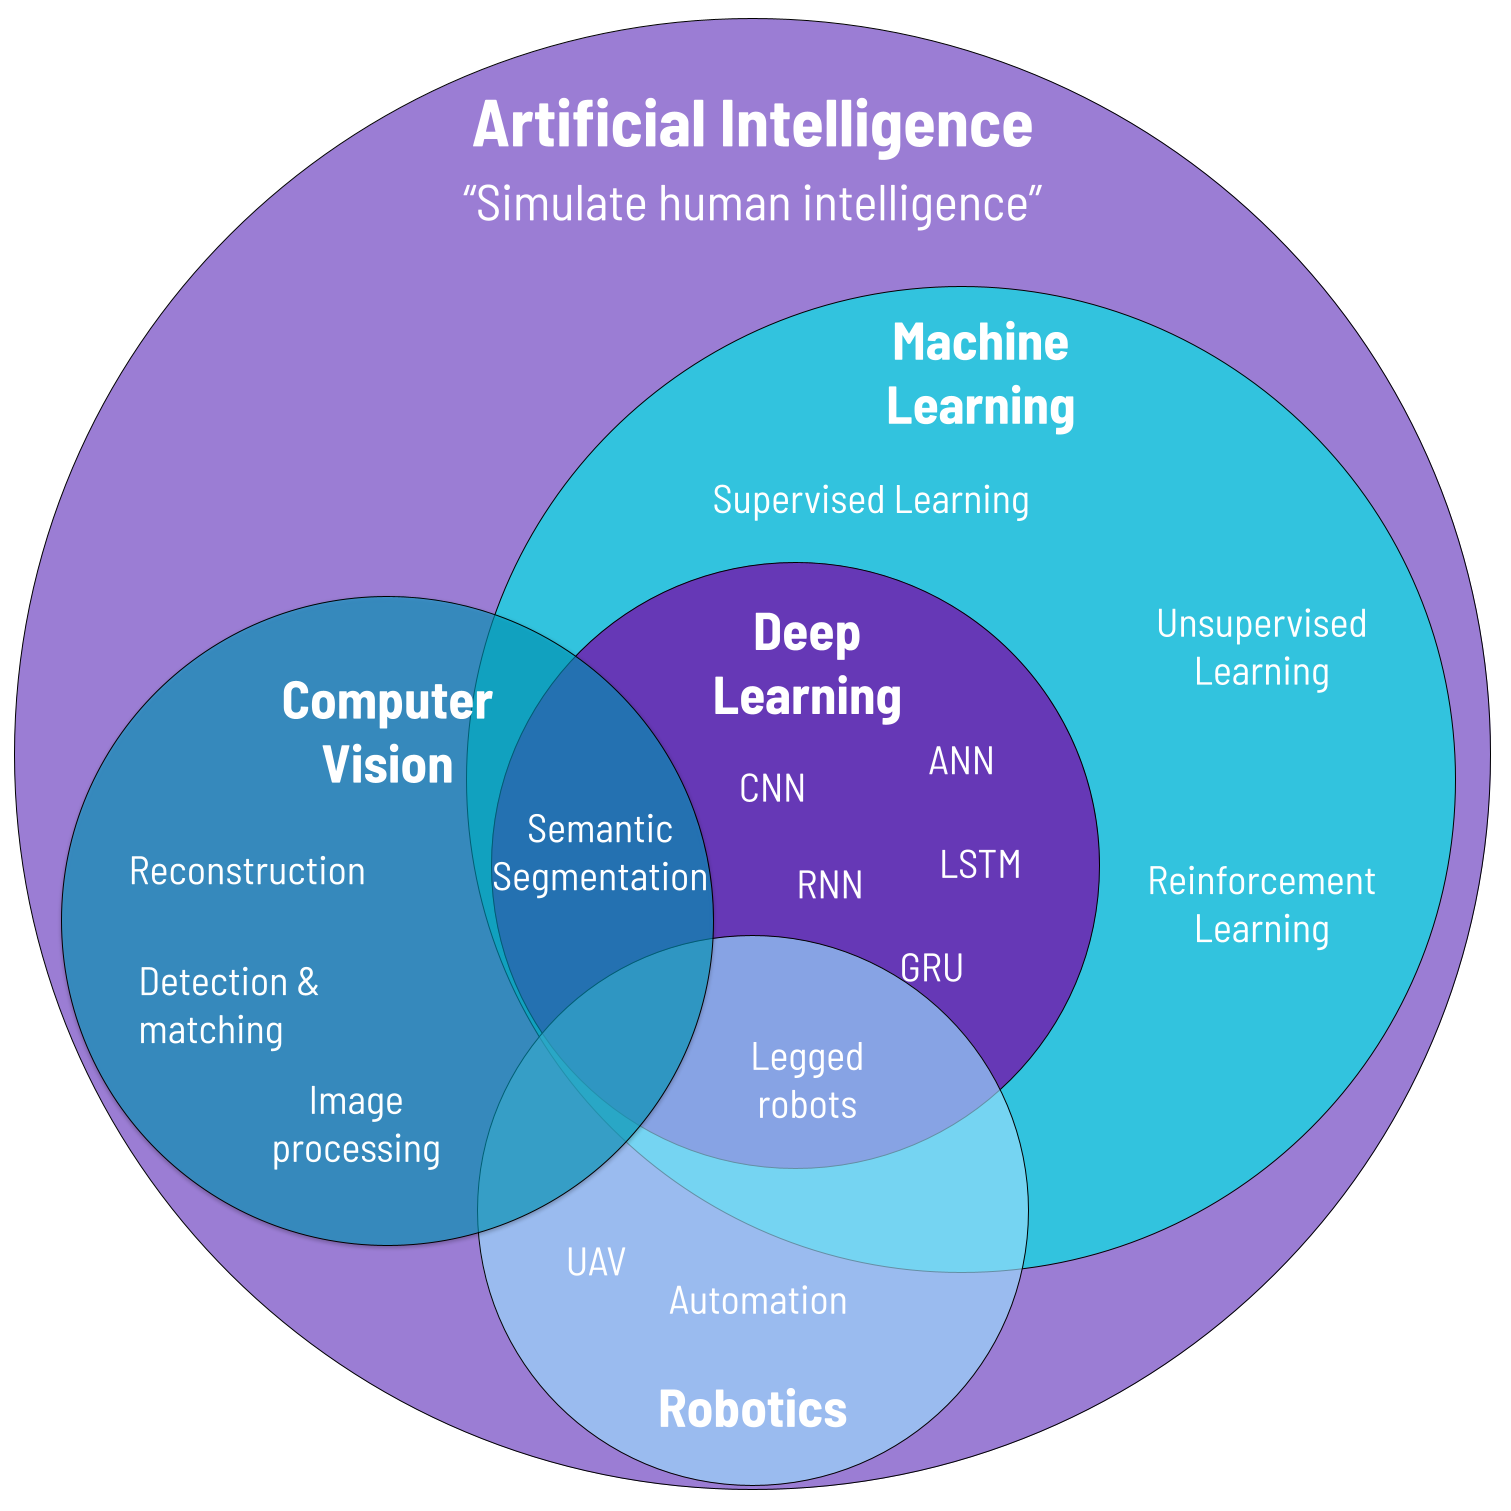
\includegraphics[width=\imgWidthM]{images/AI_Overview.png}
    \caption[\acf{AI} overview]{Overview of different techniques within the large field of \acf{AI}. The image is inspired by \cite{HUANG2021103677}.}
    \label{AI_Overview}
\end{figure}

There are several reasons why deep learning has become as popular as it is today. One reason is the increased chip processing ability which led to increased performance in parallel computing systems such as GPU clusters, or the emergence of large-scale annotated training data \cite{deng2014deep}\cite{DBLP:journals/corr/abs-1807-05511}\cite{chen2016supervised}. Additionally, there was significant research in the design of network structures and training strategies like dropout \cite{gal2016dropout}, data augmentation \cite{shorten2019survey} or batch normalization\cite{ioffe2015batch}, which led to several breakthroughs in object recognition \cite{10.1145/3448250}, speech \cite{10.1145/3448250} or video processing \cite{LeCun2015}.

One essential task relevant to this project is semantic segmentation within the \ac{ML} and deep learning field. \figref {AI_Overview} provides an overview of \ac{AI} and its most important subfields. We can see how semantic segmentation is also related to \acf{CV} intersecting with Deep Learning.

The goal of semantic segmentation is to assign a class label to each pixel in an image with numerous practical applications in various fields, such as autonomous driving, where it helps the car to understand the environment around it by segmenting objects in the scene such as roads, traffic lights, pedestrians or other vehicles and assists in deciding on how to navigate \cite{siam2018comparative} safely \cite{blum2019fishyscapes}\cite{chen2017importance}\cite{zhou2019automated}. In medical imaging where it can be used to identify and segment tumors, organs, or other structures, helping doctors to diagnose diseases accurately, plan surgeries, and monitor the clinical progress \cite{asgari2021deep}\cite{rezaei2018conditional}\cite{madani2020artificial}. In robotics, semantic segmentation can be used to help robots to interact with environments by detecting obstacles for pathfinding or for pick and place tasks \cite{milioto2018real}\cite{milioto2019bonnet}\cite{wada2019joint}. Semantic segmentation can also assist in surveillance to track and detect objects such as people \cite{jung2001content}, animals, vehicles, or cargo for logistics companies \cite{cane2018evaluating}. It can further assist in border control \cite{balado2019road}\cite{wang2022deep}, wildlife monitoring \cite{haucke2021exploiting} or crowdmanagement \cite{wan2021fine}. In the field of \acf{AR} it can be used to place virtual objects in the real world, track the objects' movements and help to make the appearance of virtual objects seamless and more natural \cite{tanzi2021real}\cite{ko2020novel}.

One crucial step in preparing data for deep learning, especially for techniques such as semantic segmentation, is to provide an accurately labeled dataset. The process involves assigning a label or tag to each data point which indicates which category or class it belongs to \cite{YU201882}. For semantic segmentation, labels consist of images with annotated pixels with a label corresponding to the object or category typically represented as integers. If no dataset is available, the labeling task requires extensive effort manually or by applying semi-automatic or automatic annotation mechanisms \cite{rapson2018reducing}\cite{sager2021survey}. For any of these techniques, providing a very high quality of the labeled data is essential as otherwise, the model will not be capable of recognizing patterns accurately \cite{alonso2015challenges}\cite{https://doi.org/10.48550/arxiv.2103.14749}. While labeling images for some fields is pretty straightforward and requires no specialist knowledge, the cost to obtain annotated images for medical image analysis is much higher \cite{willemink2020preparing}. Large labeled datasets are pretty rare; thus, extensive research has been undertaken to improve performance on small scaled or incomplete datasets \cite{Zhang2018}\cite{Barz_2020_WACV}\cite{10.1145/2818346.2830593}\cite{WANG2021102579}\cite{8693644}.

Given the importance of training with limited data, this project aims to improve segmentation performance for small datasets with biomedical imagery by proposing an end-to-end training architecture with a custom loss merging functionality. The proposed pipeline further gives the user an intuition about suitable loss combinations for any input dataset by providing a final score for combined loss functions. The architecture components are set up in a way to deal with highly unbalanced datasets, which provide additional challenges which, in practice, are very common when dealing with "real world" data \cite{DBLP:journals/corr/abs-1901-08394} \cite{DBLP:journals/corr/abs-1710-05381}.

The contribution of this project can be summarized as follows:
\begin{enumerate}
  \item \textbf{\emph{U-Net based segmentation architecture}}: Implementing a robust segmentation architecture using the U-Net model.
  \item \textbf{\emph{Baseline training}}: Training of several baseline models on three highly unbalanced datasets of different difficulties, using six distinct loss functions.
  \item \textbf{\emph{Loss function analysis}}: In-depth comparison and analysis of six standard loss functions and presentation of a method for combining them effectively.
  \item \textbf{\emph{Loss merging framework}}: Development of a fully automatic loss merging experimentation framework enabling users to add, combine easily, and weight loss functions to find the most suitable combination for a given dataset.
  \item \textbf{\emph{Insightful experimentation}}: Extensive tests to gain insight into suitable loss combinations and merging strategies for optimal performance.
  \item \textbf{\emph{Public availability}}: Deployment as a publicly available software package, allowing others to benefit from the research and findings.
\end{enumerate}

\section{Structural Design}
\chapref{chap:introduction} describes the scientific problem and goals to achieve with this project. The chapter briefly reviews semantic segmentation, its importance, and its relation within the deep learning context. The chapter closes by defining the document's contributions and structural design. \chapref{chap:fundamentals} provides an extensive review of \acf{ML}, semantic segmentation, and its relation to \acf{CV} for the reader to get a better understanding of the research problem and approach. It further introduces several segmentation objectives, metrics, the used architectures and a standard deep learning framework. \chapref{chap:literature_review} includes an extensive summary of techniques for improving segmentation with a focus on custom loss functions. \chapref{chap:methodology} describes the proposed methodology starting with an in-depth analysis of limiting factors for loss functions and then discussing numerous merging strategies to combine losses with the goal to improve segmentation performance. \chapref{chap:experimental_setup} introduces the experimental setup, including the dataset, parameter configurations, preprocessing steps, training, validation, testing, and monitoring settings, while the \chapref{chap:implementation} presents the implementation details, such as the programming language, the deep learning framework used, management tools, the network architecture, and a custom analysis spreadsheet. \chapref{chap:results} discusses the results achieved structured by dataset and \chapref{chap:discussion} summarizes the achieved results. \chapref{chap:conclusion} provides an overall reflection of the main contributions, discusses their significance, and outlines their limitations to suggest directions for future work.
\chapter{Fundamentals}
\label{chap:fundamentals}
This chapter introduces the terminology employed throughout this work, followed by a brief overview of \acf{ML} fundamentals, including supervised, unsupervised, and reinforcement learning. The focus then shifts to semantic segmentation, exploring its connection to \acf{CV}, segmentation objectives, metrics, and architectures.
\section{Terminology}
\label{sec:terminology}
This section provides the terminology used throughout this work to guarantee consistency for mathematical definitions. The terms are commonly used within \ac{ML} and have been adapted to fit the context of semantic segmentation.

\textbf{Input features $x\in X$}: Data from the input space $X$ which we want to use to make predictions for. In the case of semantic segmentation, every input $x$ can be defined as a tensor of shape $([C,H,W])$ where $C$ is the number of channels such as red-green-blue (RGB), $H$ the height and $W$ the width of the image. If we use batches of images, we describe them as a tensor of $([N,C,H,W])$ where $N$ is the number of batches.

\textbf{Output labels $y\in Y$}: Targets from the label space which we want to predict. Labels consist of tensors of shape $([N,H,W])$ where $N$ is the batch size, $H$ is the height, and $W$ is the image's width. For training, we usually convert the tensor $([N,H,W])$ into a one-hot-encoded format of shape $([N,D,H,W])$ where $D$ stands for the number of distinct classes.

\begin{figure}[H]%[htbp]
    \centering
    \subfigure[]{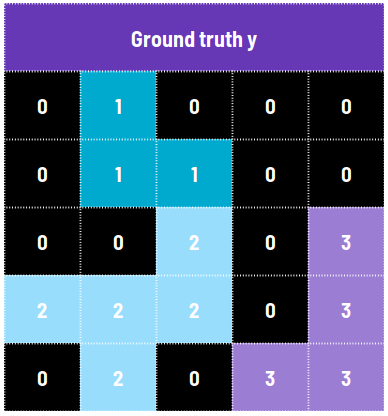
\includegraphics[width=\imgWidthFive]{images/oneHotEncoding_1.png}}
    \subfigure[]{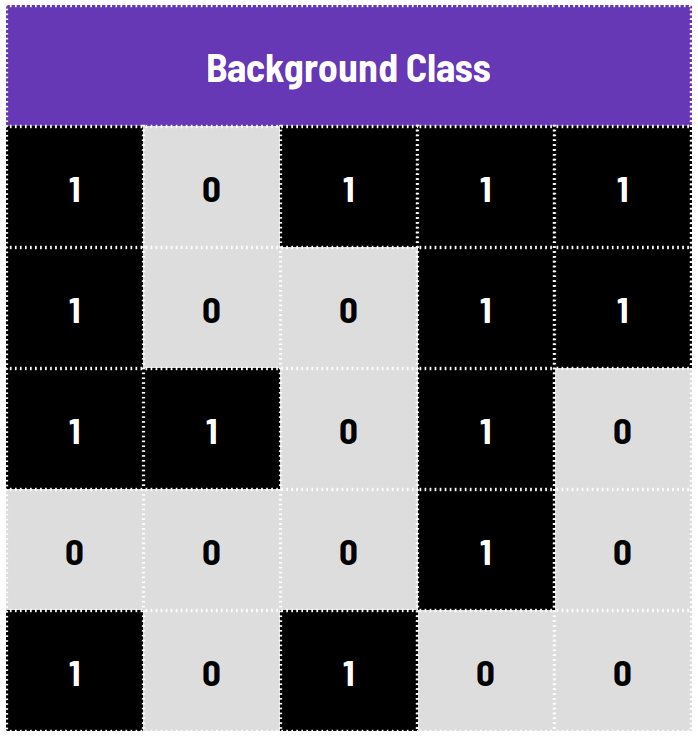
\includegraphics[width=\imgWidthFive]{images/oneHotEncoding_5.png}}
    \subfigure[]{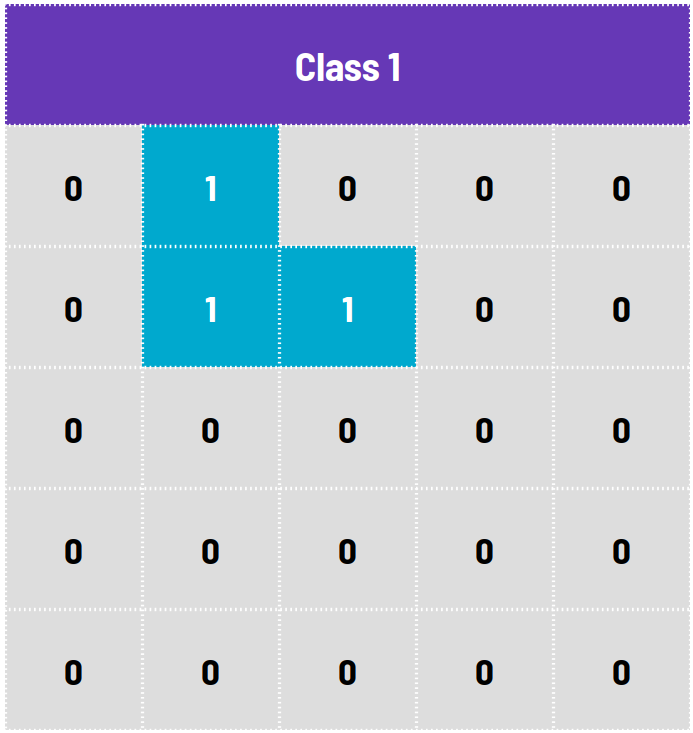
\includegraphics[width=\imgWidthFive]{images/oneHotEncoding_2.png}}
    \subfigure[]{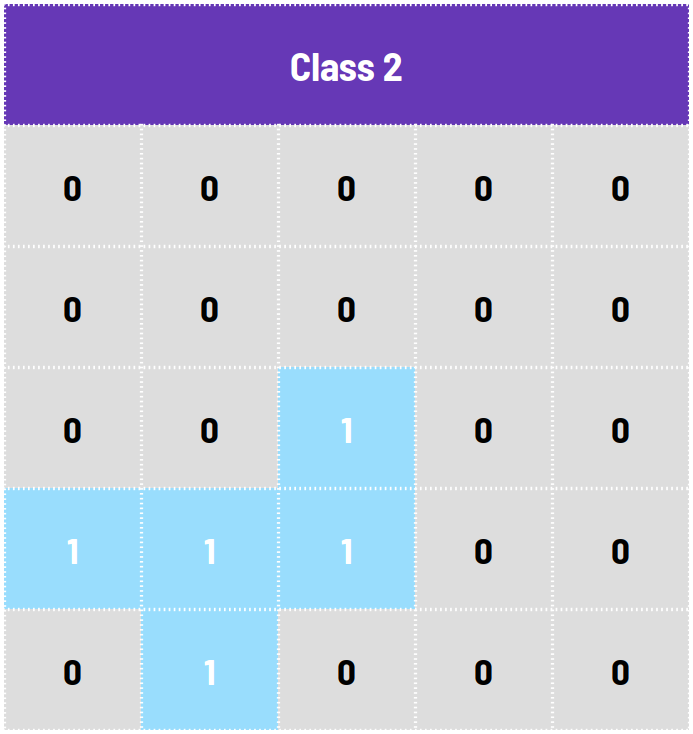
\includegraphics[width=\imgWidthFive]{images/oneHotEncoding_3.png}}
    \subfigure[]{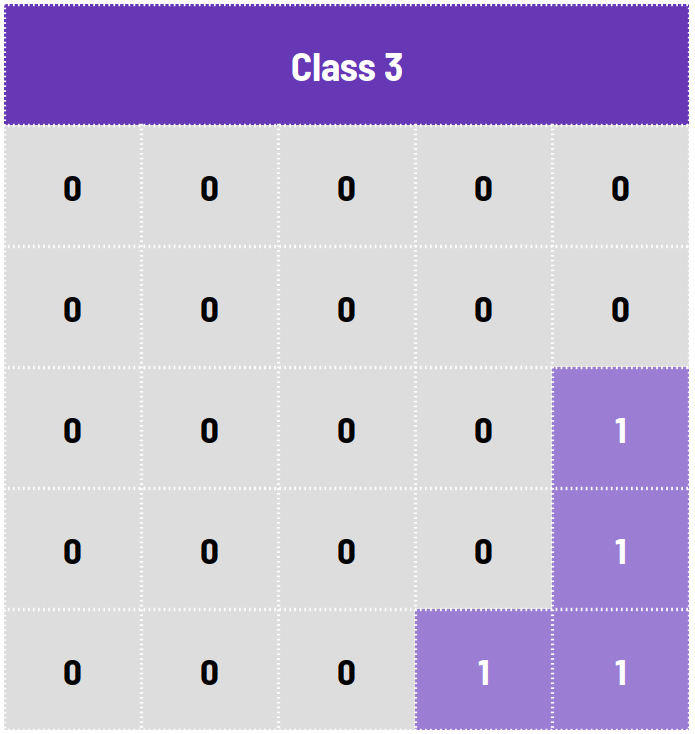
\includegraphics[width=\imgWidthFive]{images/oneHotEncoding_4.png}}
    \caption[Integer encoding $\to$ one-hot-encoding]{Example of integer-encoded output label (a) transferred to a one-hot-encoded label (b-e) of shape $([N,D,H,W])$. In this example, the batch size $N=1$}
    \label{one_hot_encoded_mask}
\end{figure}

\textbf{Probability distribution $\mathbb{P}(XY)$}: Unknown distribution of input features and output labels. A subset from this distribution would be a dataset $D=\{(x_i,y_i)\}_{i=1}^m \in (X,Y) \sim \mathbb{P}(X,Y)$.

\begin{figure}[H]%[htbp]
    \centering
    \subfigure[]{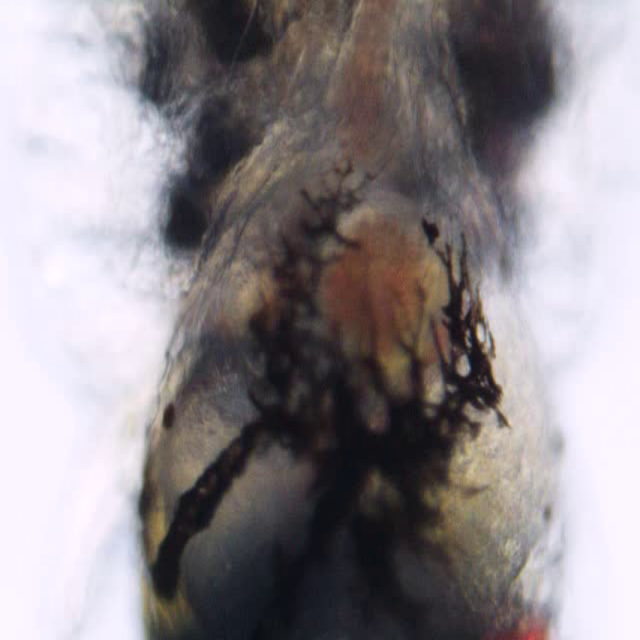
\includegraphics[width=\imgWidthTwo]{images/medaka.png}}
    \subfigure[]{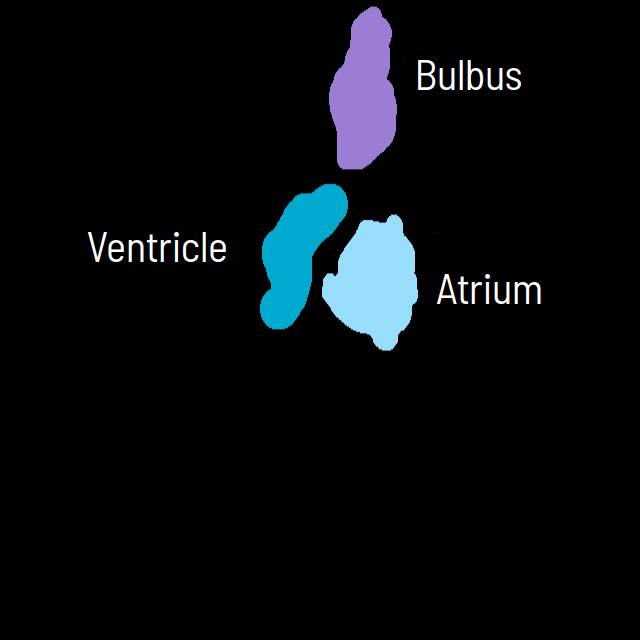
\includegraphics[width=\imgWidthTwo]{images/00020_mask.png}}
    \caption[Sample label pair]{Example of sample (a) label (b) pair $(x_1,y_1)\in (X,Y)$ of the Medaka fish dataset with four classes (Bulbus, Ventricle, Atrium, and Background)}
    \label{sample_label_pair}
\end{figure}

\textbf{Model $h_{\theta}:X \to \hat{Y}$}: Function to map features from the input space $X$ to the prediction space $\hat{Y}$ depending on $\theta$. Within semantic segmentation, $h_{\theta}$ consists of a \acf{CNN}.

\textbf{Parameters $\theta \in \Theta$}: Weights of the model which are intended to be optimized during the training phase of the model.

\textbf{Predictions $\hat{y}\in \hat{Y}$}: Outputs of the model $h_{\theta}$. The value typically consists of scores inferred from the model $h_{\theta}$. For segmentation tasks, the output shape $\hat{Y}$ is usually of the form $([N,D,H,W])$ such as $Y$, and is then optionally transformed into probabilities as defined in \secref{sec:softmax}.

\textbf{Loss function $l:\hat{Y}\times Y \to \mathbb{R}_+$}: Also known as cost function measures the difference between the prediction $\hat{Y}$ and the output label $Y$. The goal of a machine learning model is to minimize the value of the loss function by providing a gradient or direction for the model to make.


\section{Machine Learning}
\acf{ML} is a subfield of \acf{AI}. The paper \squote{Machine learning: Trends, perspectives, and prospects}\cite{doi:10.1126/science.aaa8415} provides an excellent summary of \ac{ML} and defines it as the question of \squote{How to build computers that improve automatically through experience}. The paper starts by outlining its importance as one of today's most rapidly growing technical fields and as a method of choice in \acf{CV}, \acf{NLP}, \acf{SR}, or \acf{RC}. It formally defines \ac{ML} as a learning problem to improve some measure of performance when executing some task through some training experience. Further, it describes the three most important paradigms of \ac{ML} known as \acf{SL}, \acf{UL}, and \acf{RL}.

\subsection{Supervised Learning}
\label{subsec:supervised_learning}
\acf{SL} techniques are nowadays the most widely used methods \cite{doi:10.1126/science.aaa8415}. Those methods are based on the principle known as \ac{ERM} from statistical learning theory \cite{NIPS1991_ff4d5fbb}. It is defined as an approach of the \squote{expected risk} as
\begin{equation}
    R(h_\theta)=\mathbb{E}[L(h(X),Y)]=\int L(h(X),Y) d\mathbb{P}(X,Y)
    \label{eqn:expected_risk}
\end{equation}
with the \squote{empirical risk} as
\begin{equation}
    R_\delta(h_\theta)=\int l(h_\theta(X),Y)d \mathbb{P}_\delta(X,Y)=\frac{1}{m}\sum_{i=1}^m l(h_\theta(x_i),y_i)
    \label{eqn:empirical_risk}
\end{equation}
The idea is that even if we do not know the real joint distribution of a sample, label pairs $\mathbb{P}(X,Y)$, we still can approach it with some known training data. The general goal of a \ac{SL} algorithm is to find a function $h \in H$ which models the relationship between a random feature vector $X$ and a random target vector $Y$, also called output label, by following the joint distribution $\mathbb{P}(X,Y)$. $L$ is the loss function which penalizes the differences between prediction $h(x)$ and $Y$. $\mathbb{E}[L(h(x),y)]$ is the expected loss if we obtain samples from the same distribution $\mathbb{P}(x,y)$ as the training data \cite{DBLP:journals/corr/abs-1710-09412}. The difference between \ref{eqn:expected_risk} and \ref{eqn:empirical_risk} is the distribution from where the data is sampled. While the former samples the data from the real unknown distribution $\mathbb{P}(X,Y)$, the latter is an approximation obtained from the distribution $\mathbb{P}_\delta(X,Y)$ wich represents samples from a dataset $DS=\{(x_i,y_i)\}_{i=1}^m$.

The inputs of the dataset $DS$ can have numerous forms, such as simple vectors, DNA sequences, images, or graphs \cite{doi:10.1126/science.aaa8415}. For \ac{SL} methods, the output $y$ typically is either a category used for classification or a real value for regression methods. The following section will describe some of the most essential \ac{SL} methods and briefly outline how to optimize the \squote{empirical risk} defined as \ref{eqn:empirical_risk}.

\subsubsection*{Supervised Learning Models}
\label{subsubsec:supervised_learning_models}
\textbf{\emph{\acf{LR}}} is a supervised technique used to model the relationship between a dependent and one or more independent variables. The dependent variable is a real value. Some applications for \ac{LR} are the prediction of stock prices for financial institutes \cite{bhuriya2017stock}, sales volume \cite{todua2013multiple}, customer lifetime value \cite{malthouse2005can} or churn rates \cite{hadden2008churn} for sales and marketing departments \cite{maulud2020review}, predicting patient outcomes \cite{lewis2007regression} or healthcare costs \cite{soyiri2013overview}, modeling the relationship between environmental variables such as temperature \cite{radhika2009atmospheric}, humidity \cite{vamseekrishna2021prediction} or precipitation \cite{naoum2004orographic} and their impact on natural systems for environmental scientists \cite{shen2015precipitation}. Mathematically, the linear regression model can be expressed as
\begin{equation}
    h_{\theta}(x)= \sum_{j=1}^n \theta_j x_j=\theta^T x
    \label{eqn:linear_regression}
\end{equation}
where $x$ is the dependent variable, $h_\theta(x)$ the independent variables and $n$ the number of features. $\theta$ are the coefficients or parameters. As a loss function, we could use the squared error or $l_1$ loss defined as
\begin{equation}
    l_1(h_{\theta}(x),y)=\sum_{i=1}^m(\theta^T x_i-y)^2
\end{equation}
or the absolute loss or $l_2$ as
\begin{equation}
    l_2(h_{\theta}(x),y)=\sum_{i=1}^m|\theta^T x_i-y|
\end{equation}
which is less sensitive to outliers \cite{thanoon2015robust}\cite{su2012linear}. Note that $m$ is the number of samples in the dataset.

\textbf{\emph{\acf{LogR}}} is another supervised technique but used for classification problems. The dependent variable is based on a logistic model, which typically estimates the probability of an outcome of two classes. There are many domains where \ac{LogR} can be applied. Some of them are fraud detection \cite{sahin2011detecting}, customer churn prediction \cite{de2018new}, medical diagnosis \cite{tsien1998using} or sentiment analysis \cite{ramadhan2017sentiment}. For \ac{LogR}, we can use the same linear model as defined in \ref{eqn:linear_regression} but with a different loss function as
\begin{equation}
    \begin{split}
        l_{\log}(h_{\theta}(x),y) & =\sum_{i=1}^m y_i \log(\theta^T x_i) + (1-y_i)\log(1-(\theta^T x_i))\\
        & =\sum_{i=1}^m y_i \theta^T x_i - \log(1+ \exp(\theta^T x_i))
    \end{split}
\end{equation}
which is also called the log-likelihood function \cite{hastie2009elements}.

\textbf{\emph{\acf{TBM}}} are also \ac{SL} methods which can be either used for classification or regression tasks. \ac{TBM} can be used with ensemble methods to improve performance. The core idea of ensembles is that, on average, they perform better than individual models. New predictions are then made by averaging \cite{hastie2009elements} or voting \cite{cootes2012robust}. Averaging is used for regression and voting for classification tasks. The advantage of decision trees is that they are easy to create \cite{almuallim2002development} and interpret \cite{kingsford2008decision}, that they require fewer data preparation, and that they are insensitive against outliers or missing data \cite{decisionTreesAdvantages}. Formally the model of \ac{TBM} can be described as
\begin{equation}
    h_\theta(x)=\sum_{m=1}^M c_m \mathbbm{1}\{x \in R_m\}
\end{equation}
The model consists of a sum of constants $c$, if $x$ is within a region $R_m$ of the decision tree. The constants $c_m$ here depend on the task and can be the proportion of each class $c_m=\frac{1}{N_m}\sum_{x_i \in R_m}\mathbbm{1}\{y_i=k\}$ for \acp{CT} or the mean of all labels $c_m=\frac{1}{N_m}\sum_{x_i \in R_m} y_i$ for \ac{RT} \cite{hastie2009elements}. There are numerous popular variants of decision trees such as \ac{RF} \cite{cutler2012random}, \ac{GB} \cite{ke2017lightgbm} or \ac{AB} \cite{wu2020application}.

\textbf{\emph{\acf{KNN}}} is a non-parametric \ac{SL} algorithm. \ac{KNN} can be used for either classification or regression tasks. The predictions for \ac{KNN} are made based on the voting of the majority class among its $k$ nearest neighbors in the training set \cite{doi:10.1142/S0218195905001622}. The advantages of \ac{KNN} are that it is straightforward and easy to understand, that it can achieve high accuracy by using different distance metrics \cite{Uddin2022}, that it can handle non-linear and complex data sets by using kernel functions and that it adapts to changing data distributions by updating nearest neighbors dynamically \cite{zhangzhonghengKNN}. Some disadvantages are that it is slow and computationally expensive for large datasets with many classes \cite{Uddin2022}, its sensitivity to irrelevant features \cite{zhangzhonghengKNN}, and that it suffers from the curse of dimensionality \cite{kouiroukidis2011effects}. Formally the model can be described as
\begin{equation}
    h(x)=\frac{1}{k}\sum_{x_i \in N_k(x)} y_i
\end{equation}
where $N_k(x)$ is the neihborhod of $x$ defined by the $k$ closest points $x_i$ in the data set \cite{hastie2009elements}. This model type can be used for classification where $y=\{-1,+1\}$ or regression where $y$ is a real value.

\textbf{\emph{\acfp{SVM}}} are also \ac{SL} models that can achieve good performance and generalization by using different kernels to handle different types of data and problems. The core idea of \acp{SVM} is to find a linear or non-linear function that maps the input data to a higher-dimensional space where a separating hyperplane with a maximal margin can be found. The hyperplane is defined by a set of points, called support vectors which lie on the boundary of the margin \cite{pisner2020support} \cite{Hearst1998TrendsC}. \acp{SVM} have been extensively used in multiple domains such as text categorization \cite{tong2001support}, face detection \cite{osuna1997training} or neuroimaging analysis \cite{PISNER2020101}. There are numerous types of \acp{SVM}. The soft margin support vector machine in primal form is a minimization of the objective
\begin{equation}
    \begin{split}
        \mathop{\min}_{\theta,b}\quad\quad\frac{1}{2}||\theta||^2 + C \sum_{i=1}^m \xi_i\\
        \text{subject to}\quad y_i(\theta^T f(x_i)+b)&\geq 1 -\xi_i\quad i=1,\hdots ,m\\
        \xi_i&\geq 0\quad\quad\quad i=1,\hdots,m
    \end{split}
\end{equation}
where $C$ permits training instances to be inside the margin or on the wrong side of the separating hyperplane if increased and can thus be considered a regularization term \cite{awad2015support}. $f(x)$ is the feature function projecting the inputs into a high feature space where a linear decision surface is constructed \cite{cortes1995support}.

\textbf{\emph{\acfp{NN}}} have been invented originally by Frank Rosenblatt (1963) as the multi-layer perceptron \cite{rosenblatt1958perceptron}. Deep learning as a subset of \ac{ML} uses \ac{NN} with many layers and has revolutionized the state-of-the-art in numerous fields as described in \chapref{chap:introduction}. Generally, a \ac{NN} is a universal function approximator consisting of piecewise linear components \cite{392253}. Formally the model of a simple one layer \ac{FFN} can be described as
\begin{equation}
    \begin{split}
        z_i&=\phi(c_{0i}+u_i^T X),\: i=1,\hdots,I,\\
        p_k&=b_{0k}+\theta_k^T Z,\: k=1,\hdots,K,\\
        h_k(X)&=g_k(P),\:k=1,\hdots,K,
    \end{split}
\end{equation}
where the matrices $Z=(z_1,z_2,\hdots,z_I)$ and $P=(p_1,p_2,\hdots,p_K)$ join the individual components, $K$ represents the number of target classes, and $\phi$ the activation function of the network responsible for its non-linearity \cite{hastie2009elements}. $c_{0i},i=1,\hdots,I$ and $b_{0k},k=1,\hdots,K$ are the bias terms which provides greater flexibility. $g_k$ is the output function. We can use the softmax function described in \ref{eqn:softmax} for a classification task. We would then have $g_k(P)=\sigma(P)$. On the other hand, we can use $g_k(P)=P_k$ \cite{hastie2009elements} for a regression task.

\begin{figure}[H]%[htbp]
    \centering
    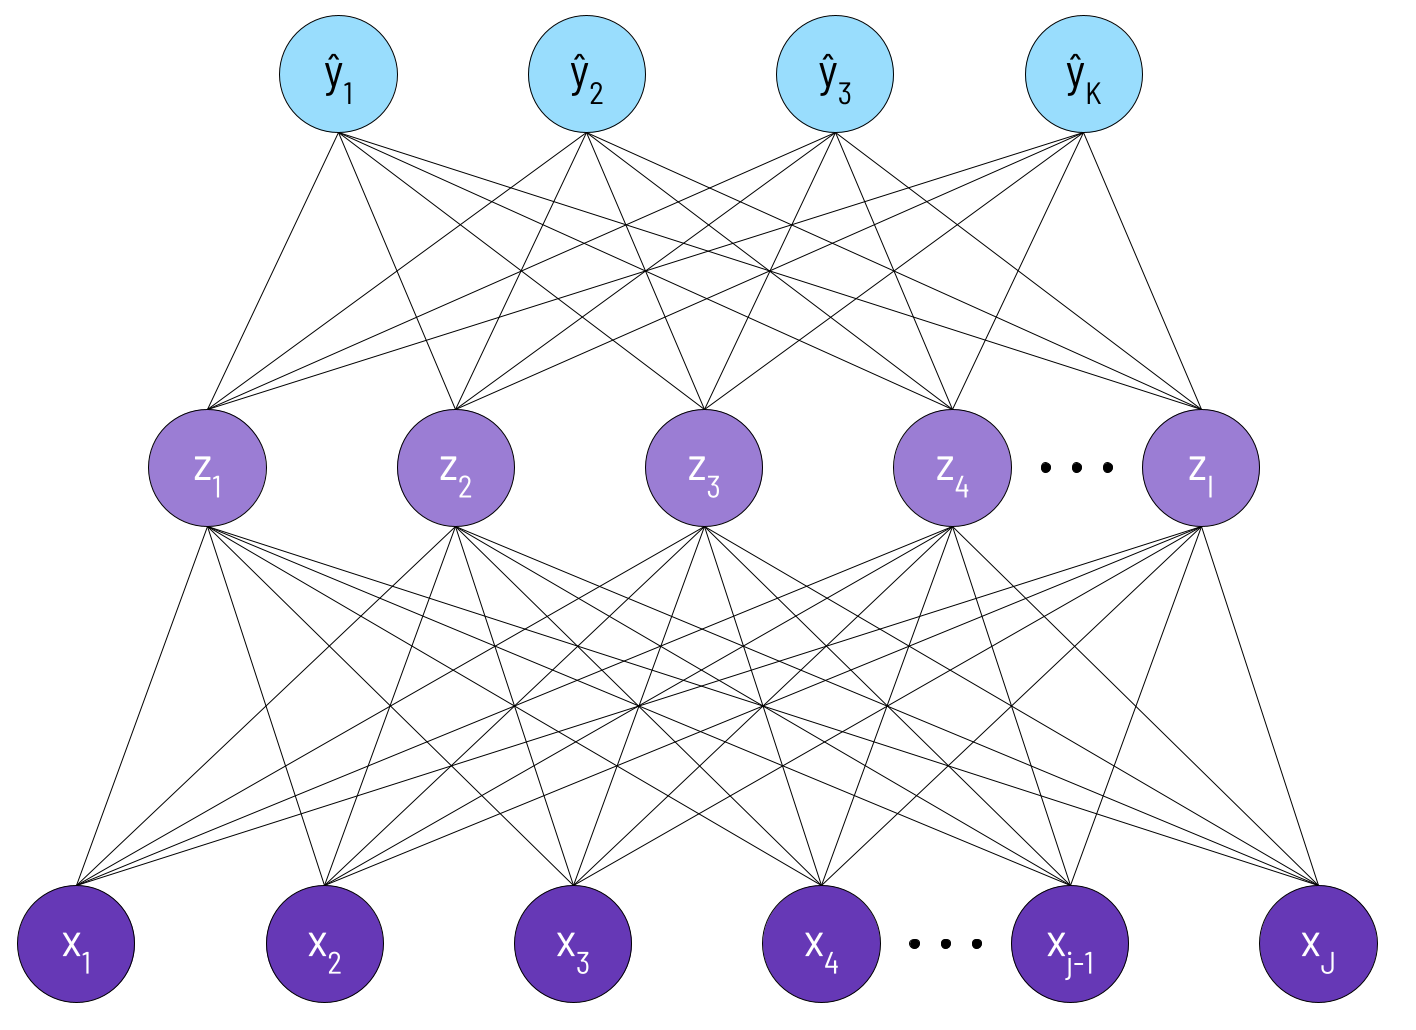
\includegraphics[width=\imgWidthL]{images/neural_network.png}
    \caption[One layered feed-forward network]{Feed forward network with one hidden layer. The illustration depicted is inspired by the schematic described in \cite{hastie2009elements}.}
    \label{neural_network}
\end{figure}
% Please add the following required packages to your document preamble:
% \usepackage[table,xcdraw]{xcolor}
% If you use beamer only pass "xcolor=table" option, i.e. \documentclass[xcolor=table]{beamer}
\begin{table}[H]
    \centering
    \begin{tabular}{|c|l|}
        \hline
        \rowcolor[HTML]{6638B6}
        {\color[HTML]{FFFFFF} Name} & \multicolumn{1}{c|}{\cellcolor[HTML]{6638B6}{\color[HTML]{FFFFFF} Formula}} \\ \hline
        Sigmoid                     & $\phi(z)=\frac{1}{1+e^{-z}}$                                                \\ \hline
        Tanh                        & $\phi(z)=\frac{e^{2z}-1}{e^{2z}+1}$                                         \\ \hline
        Relu                        & $\phi(z)=\max\{0,z\}$                                                       \\ \hline
    \end{tabular}
    \caption{List of some popular activation functions used in \acp{NN}}
    \label{tab:activation_functions}
\end{table}
Numerous activation functions are available for $\phi$, so the choice depends on data distribution, network architecture, task objective, and more \cite{DBLP:journals/corr/abs-1811-03378}. See \ref{tab:activation_functions} for a list of some popular activation functions. The ReLU activation function, for example, is widely used in hidden layers due to its simplicity and effectiveness \cite{DBLP:journals/corr/abs-2101-09957}\cite{DBLP:journals/corr/abs-2109-14545}. Generally, it is essential to add non-linearity to the \ac{NN} to make the model learn, represent and process any data and any arbitrary complex function to map inputs to outputs \cite{Sharma2020}, which on the other hand, requires minimizing an NP-hard high-dimensional non-convex objective \cite{NEURIPS2018_a41b3bb3}. This can be thought of as finding a global minimum in a chaotic, highly non-convex landscape as depicted in \figref{non_convex_landscape}.

\begin{figure}[H]%[htbp]
    \centering
    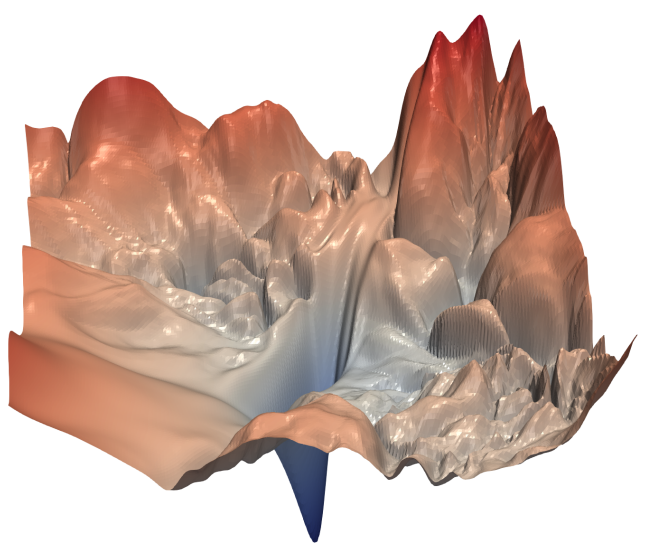
\includegraphics[width=\imgWidthM]{images/non_convex_landscape.png}
    \caption[Non-convex landscape of objective]{Highly non-convex landscape describing the complex objective of a Neural Network. The image is taken from \cite{NEURIPS2018_a41b3bb3}.}
    \label{non_convex_landscape}
\end{figure}
This section was a brief review of important \ac{SL} methods. As we can see from the definition of the \squote{empirical risk} \ref{eqn:empirical_risk}, all supervised methods require a model $h$, a set of labeled data, and some loss function typically chosen based on the task to solve, which can be a classification or regression task. Additionally, the equation \ref{eqn:empirical_risk} must be minimized, which leads to optimization theory briefly described in the next section.

\subsubsection*{Optimization}
\label{subsubsec:optimization}
As we need to minimize the \squote{empirical risk} as defined in \ref{eqn:empirical_risk} we can write the final objective as
\begin{equation}
    \mathop{\min}_{\theta} J(\theta) = \frac{1}{m}\sum_{i=1}^m l(h_{\theta}(x_i),y_i)
\end{equation}
which formally means that we want to find parameters $\theta$ that minimize the average losses of the training data.

The optimization techniques to solve this problem directly depend on the algorithm. While for some fundamental methods, such as linear regression, we can use analytic solutions, \ac{NN} requires an optimization technique called gradient descent which minimizes the objective by updating the parameters in the opposite direction of the gradient of the objective function concerning the parameters $\theta$ \cite{DBLP:journals/corr/Ruder16}. Intuitively we can think of trying to find a path to reach at least a local minimum on a non-convex surface as illustrated in \figref{non_convex_landscape}.

One of the most critical parameters in deep learning optimization is the learning rate, which controls the size of the steps taken during each iteration of the optimization process \cite{goodfellow2016deep}. A low learning rate can result in slower convergence, while a high learning rate might hinder finding an appropriate minimum. In practice, adaptive learning rate methods can automatically adjust the learning rate during training \cite{DBLP:journals/corr/abs-1212-5701}.

Gradient descent is a widely-used optimization method in deep learning, and numerous variants have been developed to improve its performance. One such variant is stochastic gradient descent (SGD), which estimates the gradient instead of calculating the true gradient. This approach often leads to faster convergence compared to traditional gradient descent \cite{bottou2012stochastic}.

\subsection{Unsupervised Learning}
\label{subsec:unsupervised_learning}
A prominent subject within \ac{ML} is \acp{UL}, which explores data to recognize inherent patterns without the guidance of predefined output labels. Two big fields of \ac{UL} are Clustering \cite{mcgregor2004flow} and Dimensionality Reduction \cite{sorzano2014survey}. Some applications of Clustering are \acp{RS} \cite{lu2012recommender}, \ac{CS} \cite{shakya2021big} and \ac{TM} \cite{perlich2014machine} and Dimensionality Reduction includes topics as \ac{FE} \cite{boutilier2009online} \ac{SD} \cite{vogelstein2014discovery} \ac{MC} \cite{fevry2018unsupervised} or \ac{BDV} \cite{keim2013big}. Numerous methods combine supervised with unsupervised techniques, such as semi-supervised, self-supervised, or weakly supervised. While semi-supervised learning uses labeled and unlabeled data, self-supervised learning attempts to generate labeled data independently, and weakly-supervised learning uses only partial information about the label \cite{9442775}. As this project focuses on \ac{SL} techniques, please refer to the keywords and papers mentioned above for further information.

\begin{figure}[H]%[htbp]
    \centering
    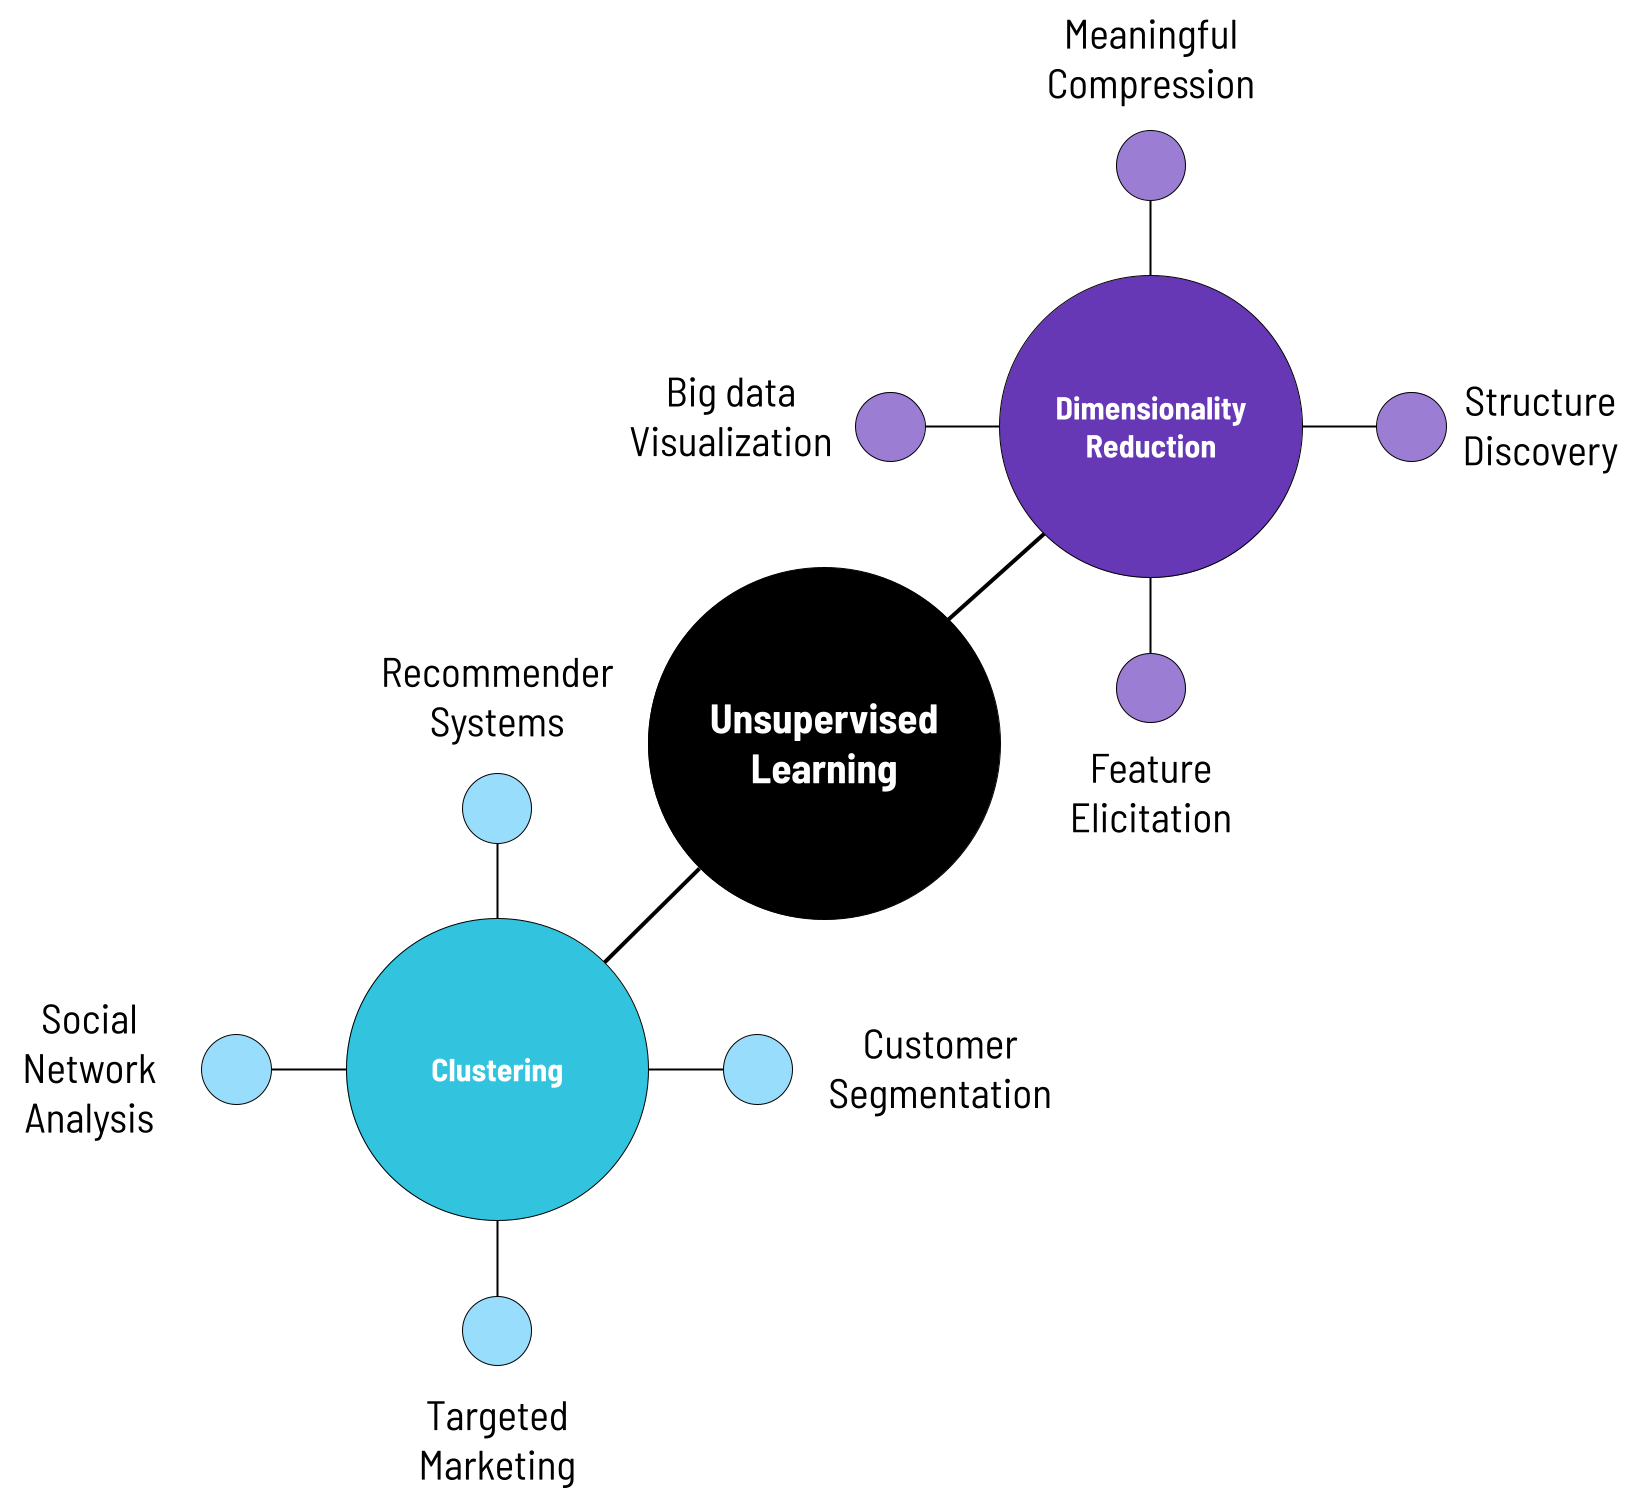
\includegraphics[width=\imgWidthM]{images/UnsupervisedLearning.png}
    \caption[Applications of \acf{UL}]{Applications of \acf{UL}. The image is inspired from \cite{unsupervisedLearning1}}
    \label{UnsupervisedLearning}
\end{figure}

\subsection{Reinforcement Learning}
Another large field of \ac{ML} is \acf{RL}, which relies on using training data to evaluate actions to take. In \ac{RL}, the correct action leads to the choice of subsequent actions. While the agent\footnote{The intelligent agent is a term used extensively in the literature. The book \cite{russel2010} defines \ac{AI} as the study of agents that receive percepts from the environment and perform actions.} is not told what actions to complete, it tries to discover what action can produce a maximum feedback signal also known as reward \cite{NIPS2013_e034fb6b}. \ac{RL}, therefore, is a trial-and-error mechanism that learns through feedback \cite{Jia2020ReviewOR}.

\figref{ReinforcementLearning} illustrates a typical concept of \ac{RL} with an agent connected to its environment via perception and action. On every step, the agent receives as input $i$ an indication of the current state of the environment. Subsequently, the agent selects an action $a$, which changes the state of the environment. This state transition is then communicated to the agent through a scalar reinforcement signal $r$. The goal for the agent is to choose actions that increase the long-run sum of values of the reinforcement signal \cite{Kaelbling1996May}.

Numerous algorithms correspond to \ac{RL}. Those include dynamic programming \cite{busoniu2017reinforcement}, Monte Carlo methods \cite{hammersley2013monte}, Q-Learning \cite{van2016deep}, TD-Learning \cite{van2013reinforcement} or Sarsa algorithms \cite{zou2019finite}.

An important domain where \ac{RL} can be applied is in robotics, where \ac{RL} can help how to grasp objects \cite{joshi2020robotic}, interact with humans \cite{akalin2021reinforcement} or other robots \cite{mataric1997reinforcement}, or navigate through difficult environments \cite{liu2020robot}. Another domain is finance, where \ac{RL} can assist in portfolio management \cite{jiang2017deep}, trading \cite{deng2016deep}, or risk management \cite{jiang2017deep}. \ac{RL} can further assist in healthcare with providing diagnosis \cite{kao2018context}, treatment recommendation \cite{gottesman2018evaluating}, drug discovery \cite{zhou2019optimization} or be used for surgical robots \cite{richter2019open}. In the gaming field, \ac{RL} can help create intelligent agents that can play games such as chess \cite{silver2018general}, Go \cite{silver2009reinforcement}, poker \cite{heinrich2016deep} or even video games \cite{shao2019survey}. Additionally, \ac{RL} can be applied to \ac{CV} tasks such as feature detection \cite{bueno2017hierarchical}, image segmentation \cite{sahba2006reinforcement}, object recognition \cite{paletta2000active} or tracking \cite{yun2017action}. \chapref{chap:literature_review} will describe in more detail of how \ac{RL} methods can improve segmentation results.

\begin{figure}[H]%[htbp]
    \centering
    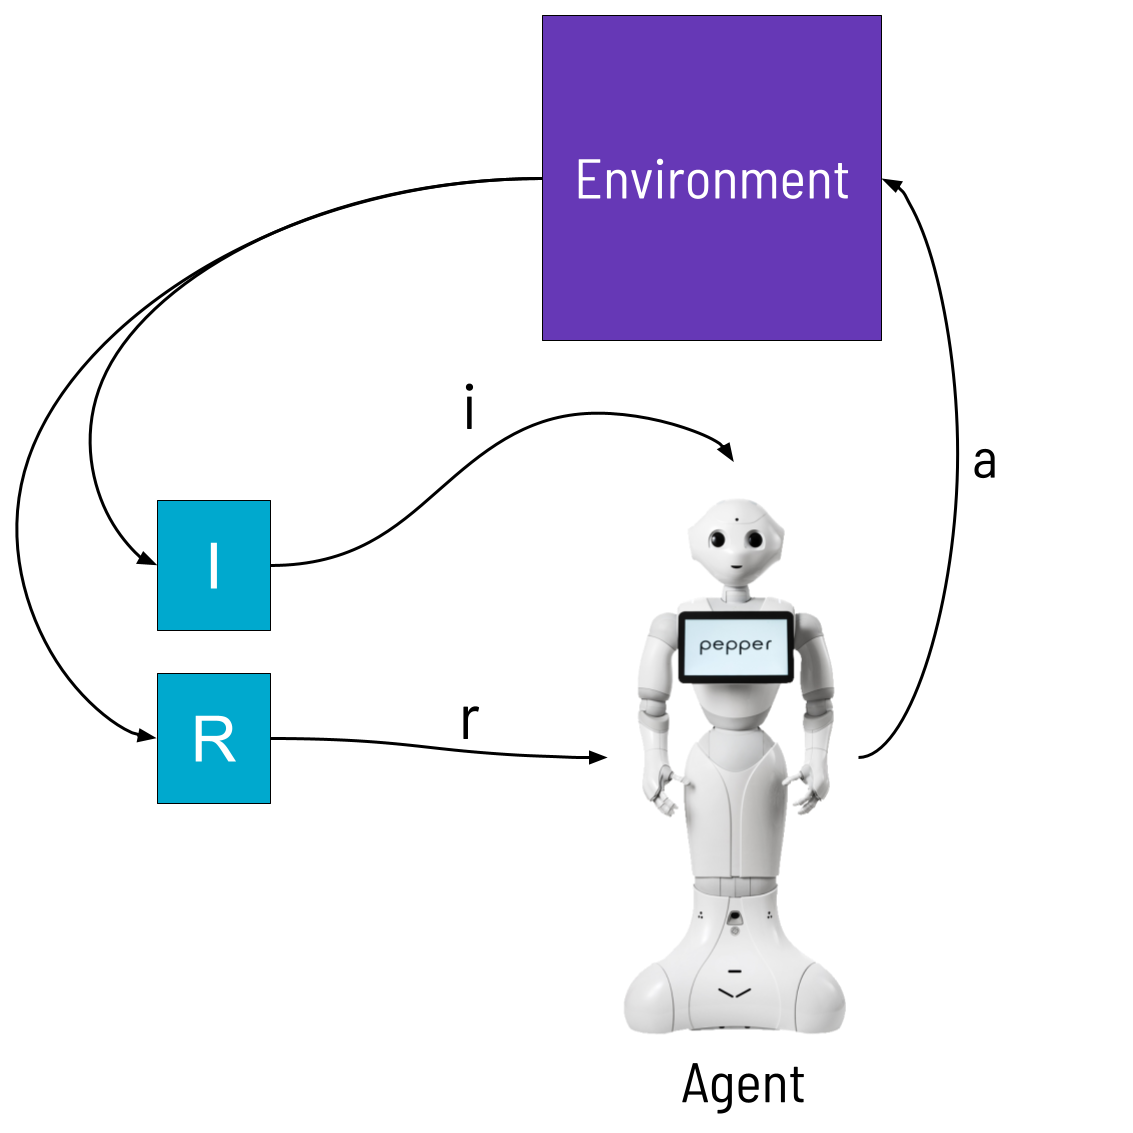
\includegraphics[width=\imgWidthM]{images/ReinforcementLearning.png}
    \caption[Concept of \acf{RL}]{Typical concept of \acf{RL} algorithm.}
    \label{ReinforcementLearning}
\end{figure}
\newpage

\begin{wrapfigure}{r}{0.4\textwidth}
    \centering
    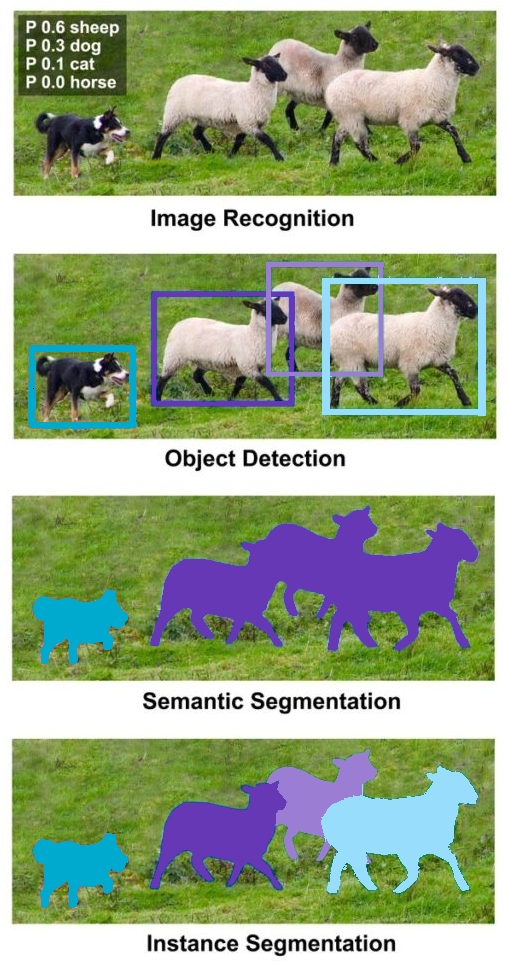
\includegraphics[width=0.30\textwidth]{images/semanticInstance_v1.jpg}
    \captionsetup{width=0.3\textwidth}
    \caption[Scene understanding]{Semantic segmentation within the context of scene understanding. Image from \cite{Bright2020Nov}.}
    \label{semanticInstance}
    \vspace{-20pt}
\end{wrapfigure}
\section{Semantic Segmentation}
This section offers a comprehensive overview of semantic segmentation using deep learning techniques. Semantic segmentation is a pixel-level classification algorithm that is crucial in comprehensively understanding images. According to \cite{GARCIAGARCIA201841}, many applications benefit from deriving insights from visual data. Notably, semantic segmentation has potential applications in a diverse range of fields, including but not limited to:

\begin{itemize}[noitemsep]
    \item Autonomous driving \cite{ess2009segmentation} \cite{feng2020deep} \cite{treml2016speeding} \cite{siam2018comparative} \cite{blum2019fishyscapes}
    \item Human-machine interaction \cite{oberweger2015hands}
    \item Computational photography \cite{yoon2015learning}
    \item Image search engines \cite{wan2014deep}
    \item Augmented reality \cite{ko2020novel} \cite{zhang2020slimmer}
    \item Medical imaging and diagnostics \cite{asgari2021deep} \cite{khan2021deep} \cite{du2020medical}
    \item Facial recognition \cite{meenpal2019facial} \cite{khan2015multi}
\end{itemize}

\figref{semanticInstance} illustrates four categories of scene understanding. \textit{Image recognition} provides a probability of objects detected within an image but does not give any information about their exact location. \textit{Object detection}, on the other hand, tries to locate and draw bounding boxes around every object in the image. \textit{Semantic segmentation} classifies pixels into preset categories. In the example shown, sheep and dogs are distinguished as separate categories. Finally, \textit{instance segmentation}, similar to semantic segmentation, can differentiate individual objects within the same class.
\subsection{Segmentation within Computer Vision}
As illustrated in \figref{AI_Overview}, semantic segmentation is a subfield of \acf{CV} and \acf{ML}. \ac{CV}, as a multidisciplinary field, encompasses a wide range of tasks and applications. Shapiro and Stockman define the objective of computer vision: \squote{The goal of computer vision is to make valuable decisions about real physical objects and scenes based on sensed images} \cite{shapiro2001computer}.

The authors describe Sensing, Encoded Information, Representations, and Algorithms as critical aspects of computer vision. \textit{Sensing} refers to how sensors acquire images and encode properties such as material, shape, illumination, and spatial relationships. \textit{Encoded Information} pertains to extracting information from images for a deeper understanding, including the geometry, texture, motion, or identity of objects. \textit{Representations} involve how images are represented for further use, considering their parts, properties, or relationships. \textit{Algorithms} describe the methods used to extract or process image information.\cite{shapiro2001computer}

\begin{figure}[H]%[htbp]
    \centering
    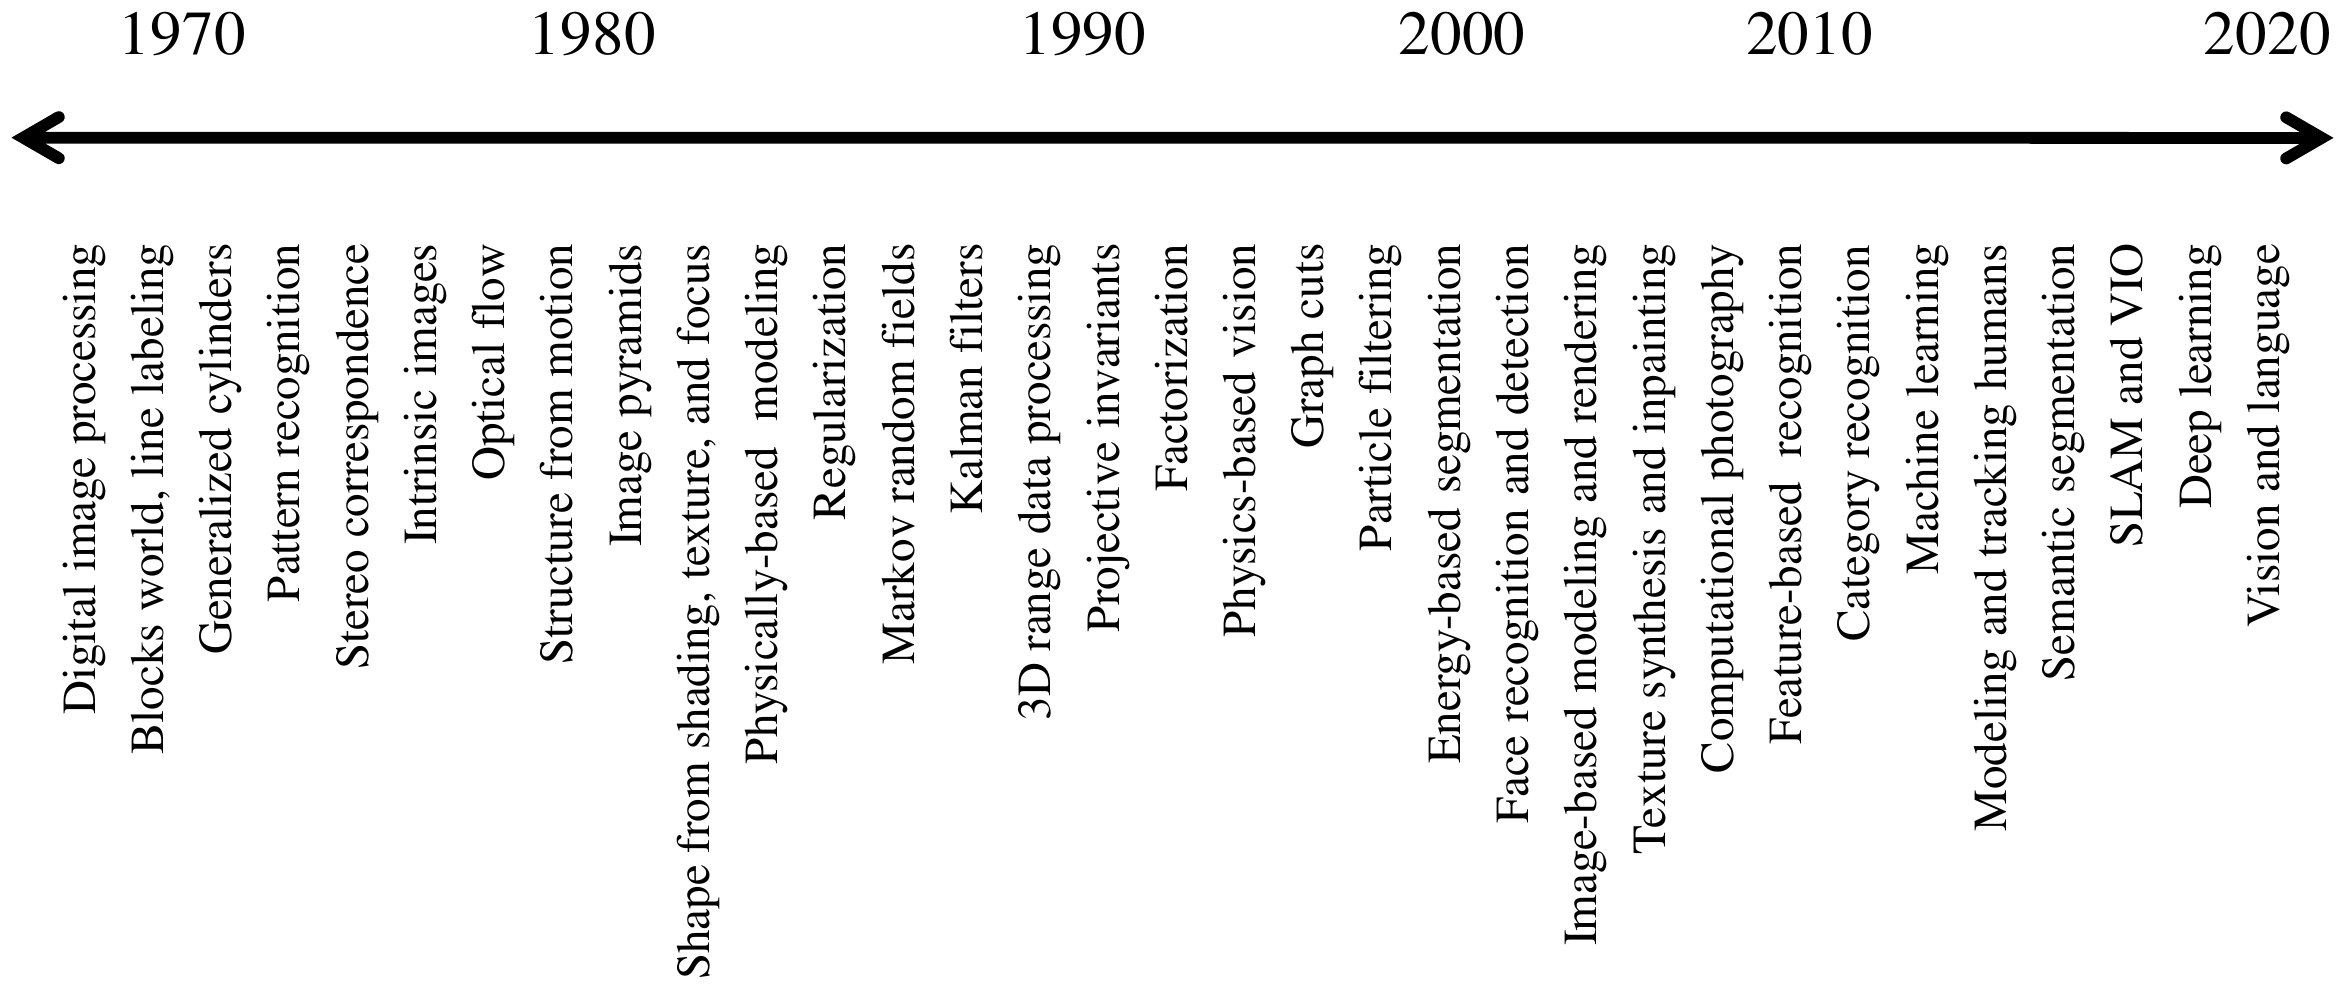
\includegraphics[width=\imgWidthXL]{images/timelineCV.png}
    \caption[Timeline of \acf{CV}]{Timeline of \ac{CV} research. Image from \cite{szeliski2022computer}}
    \label{timelineCV}
\end{figure}

Many algorithms used in computer vision were developed in studies dating back to the 1970s. \cite{szeliski2022computer} provides a fascinating timeline of the most important research topics in computer vision, as shown in \figref{timelineCV}. A significant breakthrough occurred in 2006 when Hinton introduced the Deep Belief Network with multiple layers of Restricted Boltzmann Machines. The author further states that the availability of large, public datasets and the advancement of parallel GPU computing contributed to the tremendous growth of deep learning.

The following chapter delves into some fundamental concepts of semantic segmentation, which, according to the timeline in \figref{timelineCV}, is a relatively new field within computer vision.

\subsection{Segmentation Objectives}
\label{subsec:segmentation_objectives}
As briefly mentioned above, and as illustrated in \figref{semanticInstance}, semantic segmentation aims to classify each pixel in an input image into a specific class. Applying the empirical risk introduced earlier to semantic segmentation, we have
\begin{equation}
    \mathop{\min}_{\theta} J(\theta) = \frac{1}{m}\sum_{i=1}^m l(h_{\theta}(x_i),y_i)
\end{equation}
where $m$ is the number of images in the dataset, $h_{\theta}$ the model, which typically consists of some form of \ac{CNN} architecture, $x$ the input image, $y$ the output label and $l$, the loss function which quantifies the difference between a prediction and the ground truth.

Numerous loss functions are suitable for semantic segmentation, which can be divided into different categories \cite{https://doi.org/10.48550/arxiv.2005.13449}. Subsequent sections offer an in-depth exploration of six notable loss functions, with two representatives from each category: distribution-based, region-based, and boundary-based, summarized in the following table \ref{tab:type_of_loss_functions_all}.
\begin{table}[H]
    \centering
    \begin{tabular}{|l|l|}
        \hline
        \rowcolor[HTML]{6638B6}
        {\color[HTML]{FFFFFF} \textbf{Types}} & {\color[HTML]{FFFFFF} \textbf{Names}}    \\ \hline
        Distribution-based                    & Cross-Entropy Loss (CE), Focal Loss (FL) \\ \hline
        Region-based                          & Dice Loss (DL), Tversky Loss (TL)        \\ \hline
        Boundary-based                        & Hausdorff Loss (HL), Boundary Loss (BL)  \\ \hline
    \end{tabular}
    \caption[Types of loss functions]{Types of loss functions}
    \label{tab:type_of_loss_functions_all}
\end{table}

\subsubsection*{Distribution-based}
Distribution-based loss functions focus on minimizing the dissimilarity of two distributions \cite{https://doi.org/10.48550/arxiv.2005.13449}. A principal loss function of this type is the \acf{CE}. Suppose a given segmentation task has two classes, we can use the \ac{BCE} derived from the Bernoulli distribution, and for a multi-class problem, we would use the \ac{CCE} derived from Multinoulli distribution \cite{Jadon_2020}.

\textbf{\acf{CE}}\newline
The binary cross-entropy loss can be formally defined as
\begin{equation}
    CE_{b}=-y\log(\hat{y})-(1-y)\log(1-\hat{y})
\end{equation}
For the case of multi-class classification, we would use the categorical cross-entropy loss defined as
\begin{equation}
    CE_{mc}=-\frac{1}{N}\sum_{i=1}^{N}\sum_{c=1}^C y_{i,c}\cdot \log(\sigma_{i,c})
    \label{eqn:CCE}
\end{equation}
where $N$ is the number of pixels, $C$ is the number of classes, and $\sigma_i$ is the normalized pixel with the softmax activation function as defined in \ref{eqn:softmax}.

The \ac{CE} or some variations are widely used for semantic segmentation. Prior studies claimed it works best in equal data distributions among classes \cite{Jadon_2020}. If the data is highly unbalanced, it can lead to the over-representation of larger objects in the loss, thus resulting in lower performance of smaller objects \cite{YEUNG2022102026}.

\textbf{\acf{FL}}\newline
\label{subsubsec:focal_loss}
The \ac{FL} \cite{lin2017focal} is a variant of the cross entropy loss. It provides excellent performance for highly imbalanced datasets by down-weighting easy examples and focusing on learning harder ones. The focal loss for binary classification is formally defined as
\begin{equation}
    FL_{b}=-\alpha(1-\hat{y}_t)^\gamma \cdot L_{BCE}
\end{equation}
and for multi-class classification as
\begin{equation}
    FL_{mc}=-\alpha(1-(\sigma_{i,c}))^\gamma \cdot L_{CCE}
\end{equation}
The $\alpha$ and $\beta$ parameters control how hard wrong predictions get penalized. \figref{focal_loss_plot} provides an example and the relation of \ac{FL} to \ac{CE}.

\begin{figure}[H]%[htbp]
    \centering
    \subfigure[]{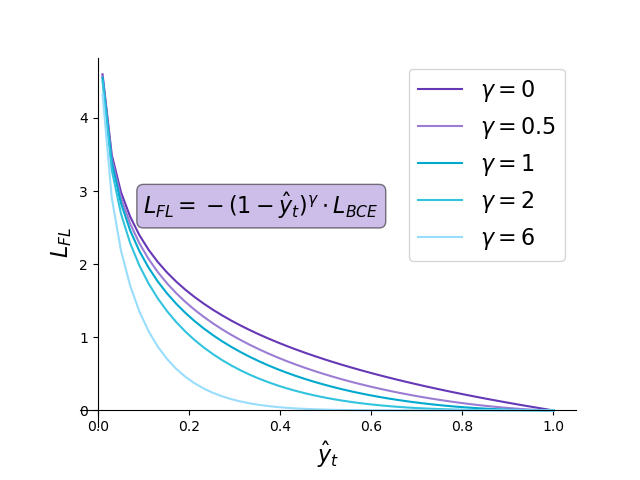
\includegraphics[width=\imgWidthTwo]{images/focal_loss_plot.png}}
    \subfigure[]{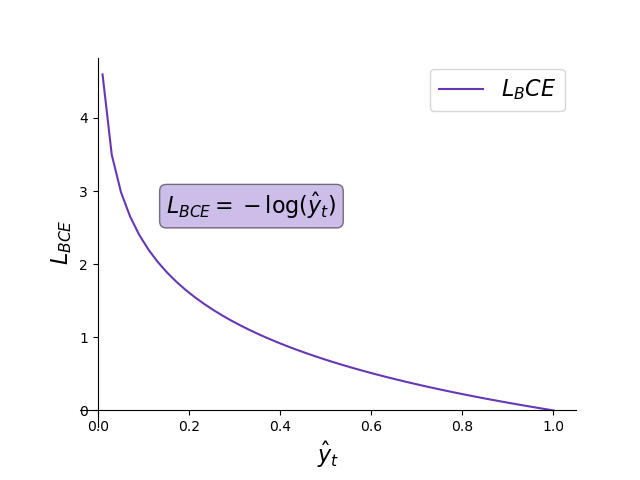
\includegraphics[width=\imgWidthTwo]{images/ce_loss_plot.png}}
    \caption[Graph of \acf{CE} and \acf{FL}]{\ac{FL} (a) as proposed in \cite{lin2017focal} with different values of $\gamma$. Whenever $\gamma=0$ focal loss turns into the regular \ac{CE} (b). Increasing $\gamma$ reduces the loss for well-classified examples, e.g., $\hat{y}_t > 0.6$ leading to a higher focus on misclassifications for hard examples.}
    \label{focal_loss_plot}
\end{figure}

\subsubsection*{Region-based}
\label{subsec:region_based}
Region-based loss functions primarily focus on the segmented regions within an image to ensure that the predicted output accurately captures the distinct areas or objects of interest. Region-based loss functions are also considered a prevalent type used in computer vision tasks such as semantic segmentation or object detection. The main difference between region-based and distribution-based loss functions is how they measure the difference between $\hat{y}$ and $y$. While region-based loss functions penalize incorrect classifications of individual pixels or regions, distribution-based loss functions penalize differences between the distribution of predicted class labels and ground truth labels.

\textbf{\acf{DL}}\\
\label{subsubsec:dice_similarity_coefficient_loss}
A popular region-based loss function for medical segmentation is the \acf{DL} based on the \ac{DSC}. The \ac{DSC} is defined as
\begin{equation}
    DSC= \frac{2|\hat{y} \cap y|}{|\hat{y}|+|y|}
    \label{eqn:dsc}
\end{equation}
where $\hat{y}$ is the set of predicted pixels and y the set of actual pixels. The numerator represents two times the cardinality of the intersection of the predicted and the actual set while the denominator is the sum of the predicted and actual cardinality.

As the \ac{DSC} is defined as a discrete set operation that is not differentiable \cite{9338261}, it cannot be directly used for training. To obtain a probabilistic version of the \ac{DSC}, an approximation known as the \ac{DL} was designed. The \ac{DL} penalizes the pixel-wise mismatch between a predicted map $\hat{y}$ and its corresponding ground truth $y$ for each class j. It is defined as
\begin{equation}
    DL=1-\frac{2\sum_{i=1}^P\sum_{j=1}^C y_{i,j} \hat{y}_{i,j}+\epsilon}{\sum_{i=1}^P\sum_{j=1}^C(y_{i,j}+\hat{y}_{i,j})+\epsilon}
\end{equation}
where $P$ is the number of pixels, $C$ the number of classes and $\epsilon$ a smoothing constant to avoid division by zero.

There are numerous variations of the dice loss. \cite{Sudre_2017} from 2017 introduces the \ac{GDL} which has the form
\begin{equation}
    GDL=1-2\frac{\sum_{l=1}^2 w_l\sum_{n y_{ln}\hat{y}_{ln}}}{\sum_{l=1}^2 w_l\sum_n y_{ln}+\hat{y}_{ln}}
    \label{eqn:gdl}
\end{equation}
where $w_l$ can provide invariance to specific label set properties by correcting the contribution of each label by the inverse of its volume. This technique can reduce the correlation between region size and dice score, which will be further discussed in \secref{sec:limiting_factors}.

\textbf{\acf{TL}}\newline
\label{subsubsec:tversky_loss}
\label{subsec:tversky}
The \ac{TL}, presented by \cite{DBLP:journals/corr/SalehiEG17a} was inspired by the Tversky index \cite{tversky1977features} from 1977 defined as
\begin{equation}
    S(\hat{y},y,\alpha,\beta)=\frac{|\hat{y} \cap y|}{|\hat{y} \cap y|+\alpha|\hat{y}\setminus y|+\beta|\hat{y}\setminus y|}
\end{equation}
where $\hat{y}$ and $y$ are sets of predicted and ground truth labels, respectively, and $\alpha$ and $\beta$ are hyperparameters that control the trade-off between false positives and false negatives.

The \ac{TL} aims to address the problem of high-precision, low-recall segmentations that can occur in highly imbalanced datasets. See \figref{precision_recall}. The authors claim this is an undesired property, especially in computer-aided diagnosis or clinical decision support systems where high recall is often more important than high precision.

The \ac{TL} is defined as follows:
\begin{equation}
    TL(\alpha,\beta)=\frac{\sum_{i=1}^N \sigma_{1i}y_{1i}}{\sum_{i=1}^N \sigma_{1i}y_{1i}+\alpha\sum_{i=1}^N \sigma_{1i}y_{0i}+\beta\sum_{i=1}^N \sigma_{0i}y_{1i}}
\end{equation}
where $\sigma_{0i}$ defined in \ref{eqn:softmax} is the probability of pixel $i$ to be part of the background region and $\sigma_{1i}$ the probability of pixel $i$ to be part of the foreground. $y_{1i}$ is 1 for a foreground pixel and $0$ for a background pixel. $y_{0i}$ would be 0 for a foreground pixel and $1$ for a background pixel. With $\alpha = \beta = 1$ the second term of the denominator would calculate the false positive rate and the second term the false negative rate. The hyperparameters $\alpha$ and $\beta$ control the balance between false positives and false negatives, with higher values of $\beta$ emphasizing false negatives and increasing recall.

\begin{figure}[H]%[htbp]
    \centering
    \subfigure[]{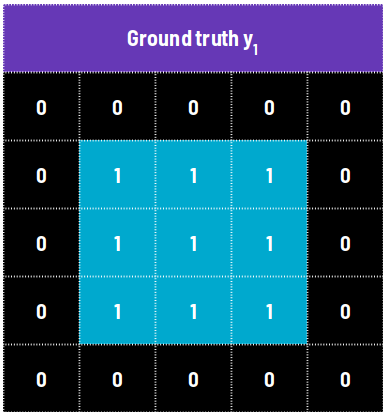
\includegraphics[width=\imgWidthFour]{images/tversky_high_precision_low_recall_y.png}}
    \subfigure[]{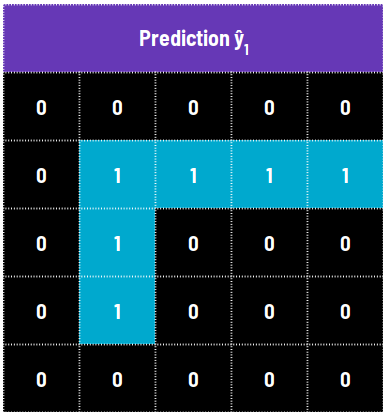
\includegraphics[width=\imgWidthFour]{images/tversky_high_precision_low_recall_yhat.png}}
    \subfigure[]{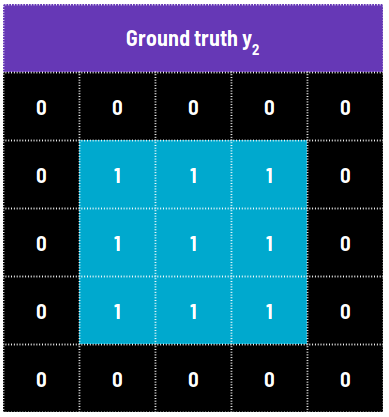
\includegraphics[width=\imgWidthFour]{images/tversky_low_precision_high_recall_y.png}}
    \subfigure[]{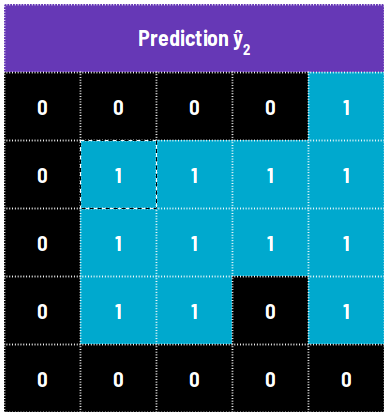
\includegraphics[width=\imgWidthFour]{images/tversky_low_precision_high_recall_yhat.png}}
    \caption[Precision and Recall]{Images (a) and (b) exhibit high precision $0.83$ with a low false positive rate and low recall $0.55$ with a high false negative rate, whereas images (c) and (d) show the opposite situation with low precision $0.61$ and a high false positive rate and high recall $0.88$ with a low false negative rate.  In heavily imbalanced datasets with a much smaller foreground class than the background class, it is common to encounter situations with high precision and low recall, resulting in many false negative classifications. This result is a critical problem in tasks such as medical image analysis, where detecting abnormalities is more important than achieving high precision \cite{powers2020evaluation}.}
    \label{precision_recall}
\end{figure}

\subsubsection*{Boundary-based}
\label{boundary_based}
Boundary-based loss functions represent a specialized type of loss functions that offers supplementary distance information, addressing the limitations of region-based and distribution-based loss functions. This section comprehensively analyzes two prominent boundary-based loss functions: \ac{BL} and \ac{HL}.

\textbf{\acf{HL}}\newline
\label{subsubsec:hausdorff_loss}
The Hausdorff loss was presented in the paper \squote{Reducing the Hausdorff Distance in Medical Image Segmentation with Convolutional Neural Networks}\cite{8767031} aiming to reduce an approximation of the \ac{HD}. The authors claim that the \ac{HD} is one of the most informative and useful objective criteria as an indicator for the largest segmentation error. The \ac{HD} was first introduced in the book called \squote{Grundz{\"u}ge der Mengenlehre} by Felix Hausdorff in the year 1914. Applied to the definitions of $y$ and $\hat{y}$ presented in \secref{sec:terminology}, defining their corresponding boundaries as $Y_b$ and $\hat{Y}_b$ the calculation for the one-sided \ac{HD} from the pointset $\hat{Y}_b$ to $Y_b$ is defined as follows \cite{rockafellar2009variational}:
\begin{equation}
    hd(\hat{Y}_b,Y_b)=\mathop{\max}_{\hat{y}_b \in \hat{Y}_b}\mathop{\min}_{y_b \in Y_b}||\hat{y}_b - y_b||_2
\end{equation}
and from the set $Y_b$ to $\hat{Y}_b$ as
\begin{equation}
    hd(Y_b,\hat{Y}_b)=\mathop{\max}_{y_b \in Y_b}\mathop{\min}_{\hat{y}_b \in \hat{Y}_b}||\hat{y}_b - y_b||_2
\end{equation}
\begin{figure}[H]%[htbp]
    \centering
    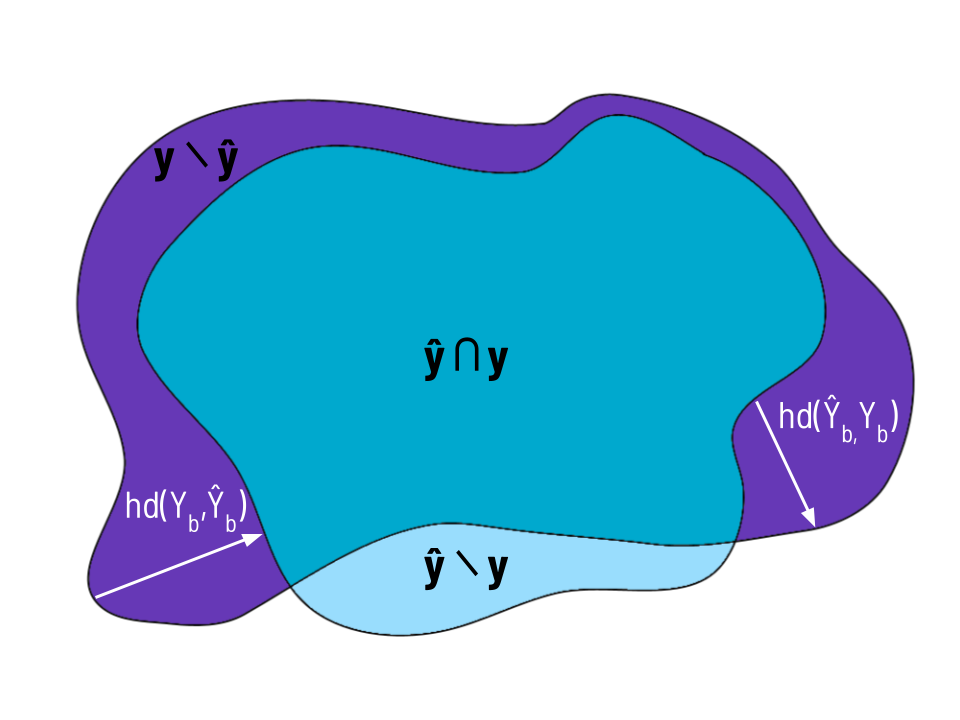
\includegraphics[width=0.5\textwidth]{images/Hausdorff_distance.png}
    \caption[Hausdorff distance]{Visual concept of the Hausdorff distance and some related notation. The two distances $hd(\hat{Y}_b,Y_b)$ and $hd(Y_b,\hat{Y}_b)$ represent the two largest segmentation errors from both the prediction boundary and output label boundary perspective. The contour additionally displays \textbf{\textcolor{rwucyan40}{false positives}} as $\hat{y}\setminus y$, \textbf{\textcolor{rwuviolet}{false negatives}} as $y\setminus\hat{y}$ and \textbf{\textcolor{rwucyan}{true positives}} as $\hat{y}\cap y$. The image is inspired by the visuals of \cite{8767031}}
    \label{Hausdorff_distance}
\end{figure}
When calculating $hd(\hat{Y}_b,Y_b)$, we can intuitively say that for every point $\hat{y}_{b,i}$ on the boundary $\hat{Y}$ we calculate the closest distance to the boundary $Y_b$ and then chose the largest value from all those closest distances. As we can see in the \figref{Hausdorff_distance}, $hd(y_b,\hat{y}_b)\neq hd(\hat{y}_b,y_b)$ which should be true in most cases. A bidirectional version of \ac{HD}, is defined as \cite{8767031}:
\begin{equation}
    HD(Y_b,\hat{Y}_b)=\max(hd(\hat{Y}_b,Y_b),hd(Y_b,\hat{Y}_b))
    \label{eqn:hd_bidirectional}
\end{equation}

The calculation of the \ac{HD} for segmentation purposes is shown to be done with the help of the distance transform method \cite{8767031}. The distance transform technique calculates the distance to a curve or a set of points using a two-pass raster algorithm \cite{szeliski2022computer}. Adjusted to the notation of the current work, the formal definition for the distance transform applied to the prediction $\hat{y}$ is defined as:
\begin{equation}
    D_{\hat{y}}(i,j)=\mathop{\min}_{k,l\:\hat{y}[k,l]=1} d(i-k,j-l)
    \label{eqn:distance_transform_yhat}
\end{equation}
or for $y$ as
\begin{equation}
    D_{y}(i,j)=\mathop{\min}_{k,l\:y[k,l]=1} d(i-k,j-l)
    \label{eqn:distance_transform_y}
\end{equation}
Note that we assume that the input, whether from $y$ or $\hat{y}$, is provided as a binary image. The equations \ref{eqn:distance_transform_yhat} and \ref{eqn:distance_transform_y} calculate the distance for every pixel to the nearest pixel with the value 1. \figref{hausdorff_dt} provides an example calculation for $D_{\hat{y}}(i,j)$ and $D_{y}(i,j)$ with input shape of $([1,1,5,5])$ for $y$ and $\hat{y}$.

\begin{figure}[H]%[htbp]
    \centering
    \subfigure[]{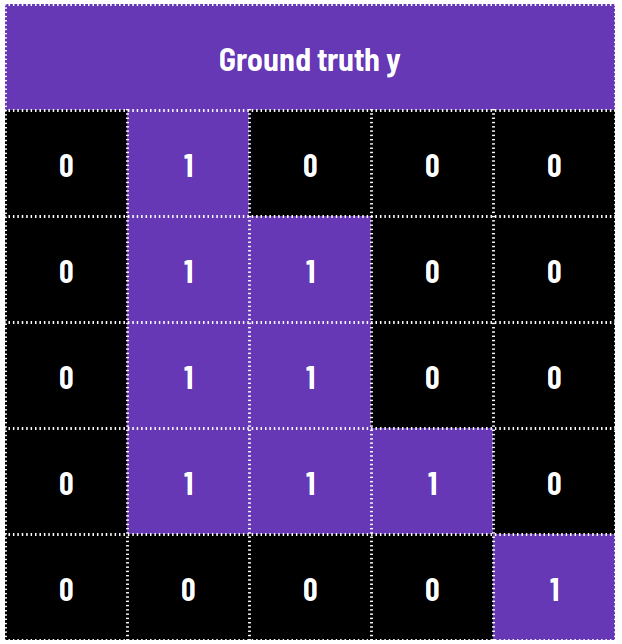
\includegraphics[width=\imgWidthFour]{images/hausdorff_y.png}}
    \subfigure[]{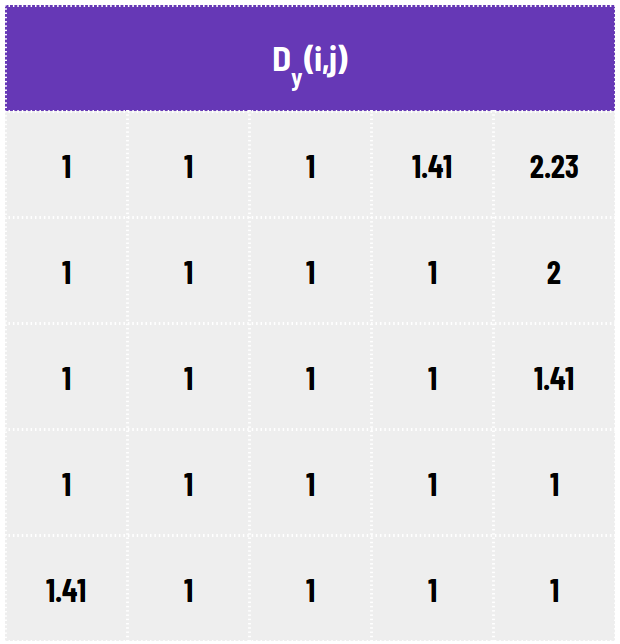
\includegraphics[width=\imgWidthFour]{images/hausdorff_dt_y.png}}
    \subfigure[]{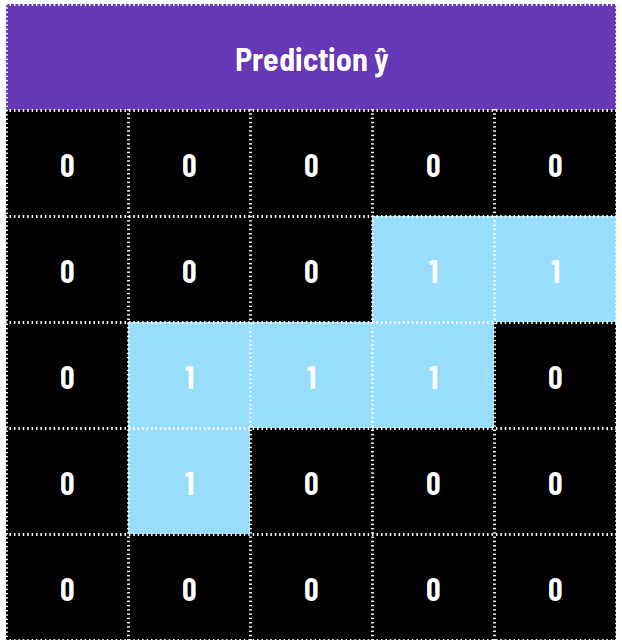
\includegraphics[width=\imgWidthFour]{images/hausdorff_yhat.png}}
    \subfigure[]{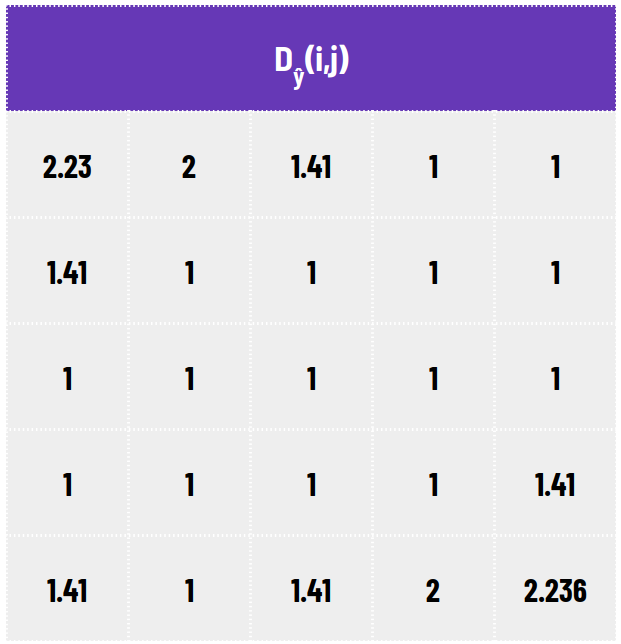
\includegraphics[width=\imgWidthFour]{images/hausdorff_dt_yhat.png}}
    \caption[Distance transform calculation]{Distance transform calculation for ground truth $y$ (a) and $\hat{y}$ (c). We can see that $D_y$ (b) and $D_{\hat{y}}$ (d) contain values that consist of distances. The position of these distances corresponds to the same position of the input $y$ and $\hat{y}$ and the distances indicate how far this pixel was from the closest pixel with the value 1.}
    \label{hausdorff_dt}
\end{figure}
For the final calculation of the \ac{HD} for segmentation, we first have to subtract $y$ from $\hat{y}$ or vice versa and then take the absolute value from the result. We still input the binary maps of $y$ and $\hat{y}$. The result will highlight false positives and false negatives as a new binary map defined as $|y-\hat{y}|$ or in set notation $y\setminus\hat{y}\cup\hat{y}\setminus y$. See \figref{hausdorff_y_minus_yhat}  or \figref{Hausdorff_distance} for further information. To finalize we need calculate $hd_D(Y_b,\hat{Y}_b)$ as
\begin{equation}
    hd_D(Y_b,\hat{Y}_b)=\mathop{\max}_{\Omega}(|y-\hat{y}|\circ D_{\hat{y}}(i,j))
\end{equation}
and $hd_D(\hat{Y}_b,Y_b)$ as
\begin{equation}
    hd_D(\hat{Y}_b,Y_b)=\mathop{\max}_{\Omega}(|y-\hat{y}|\circ D_{y}(i,j))
\end{equation}
The subscript $D$ on $hd_D$ indicates that we use the distance transform for this type of calculation. $\circ$ stands for the Hadamard product, an element-wise product of two matrices of the same size \cite{horn1990hadamard}. $\Omega$ represents the grid where the image is established, indicating that the maximum value pertains to all the pixels. \figref{hausdorff_y_minus_yhat} provides the result of the example calculation from above. For the bidirectional version, we could take \ref{eqn:hd_bidirectional} as the final loss definition.
\begin{figure}[H]%[htbp]
    \centering
    \subfigure[]{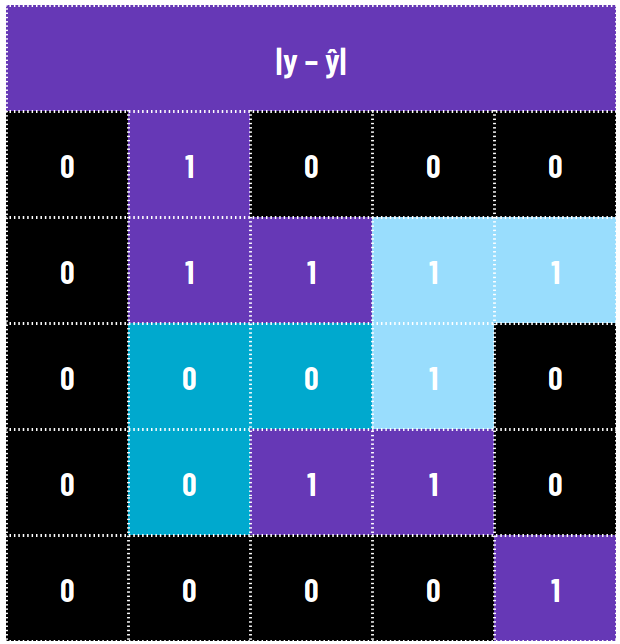
\includegraphics[width=\imgWidthThree]{images/hausdorff_y_minus_yhat.png}}
    \subfigure[]{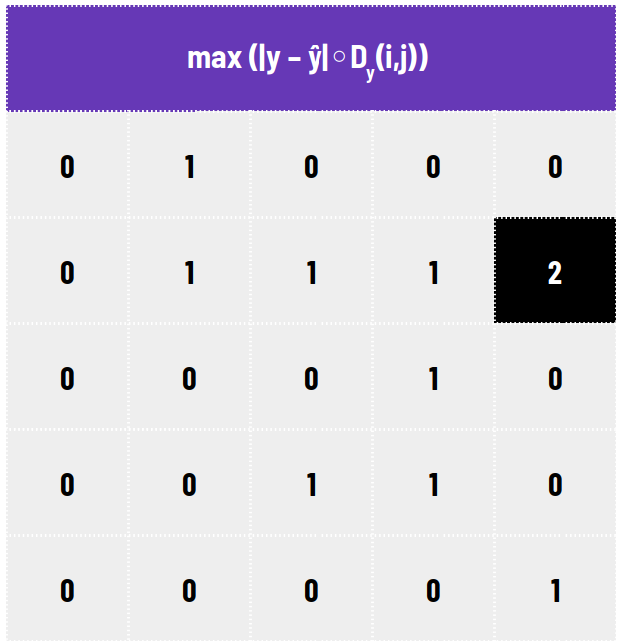
\includegraphics[width=\imgWidthThree]{images/hausdorff_max_y.png}}
    \subfigure[]{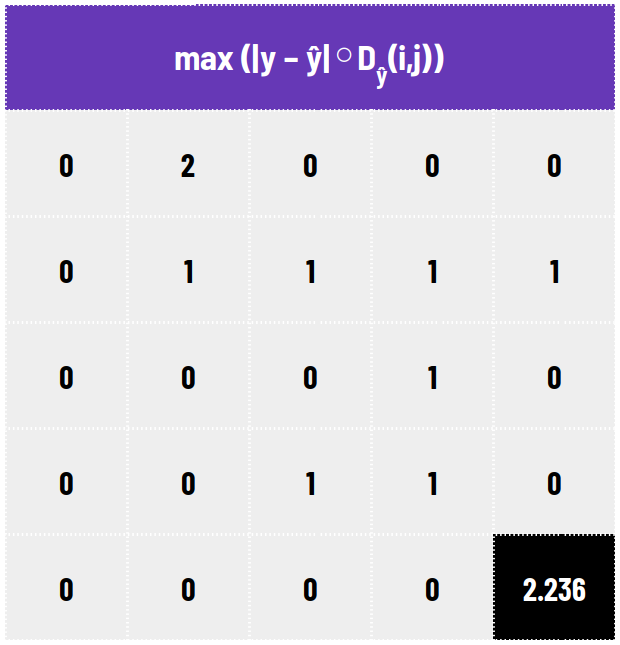
\includegraphics[width=\imgWidthThree]{images/hausdorff_max_yhat.png}}
    \caption[Hausdorff calculation result]{Image (a): \textbf{\textcolor{rwuviolet}{False negatives}}: Values predicted mistakenly as zero. \textbf{\textcolor{rwucyan40}{False positives}}: Values predicted mistakenly as 1. \textbf{\textcolor{rwucyan}{True positives}}: Correctly predicted values.The values containing one can also be described in set notation as $y\setminus\hat{y}\cup\hat{y}\setminus y$. Image (b-c): Result of the final calculation of $hd_D(Y_b,\hat{Y}_b)$ and $hd_D(\hat{Y}_b,Y_b)$.}
    \label{hausdorff_y_minus_yhat}
\end{figure}
Even if reducing the \ac{HD} directly sounds plausible, the definition \ref{eqn:hd_bidirectional} has some drawbacks. The authors of \cite{8767031} describe some disadvantages due to the limited focus on the largest distance between the boundaries, which can lead to unstable behavior in other regions. The paper refers to other works that attempted to use the \ac{HD} where most studies focus on restricted tasks such as face detection or object matching. To improve stability by focusing on the entire region of $y\setminus\hat{y}\cup\hat{y}\setminus y$, the paper proposes the following loss:
\begin{equation}
    HL(\hat{y},y)=\frac{1}{|\Omega|}\sum_{\Omega}((y-\hat{y})^2\circ (D_y^{\alpha} + D_{\hat{y}}^{\alpha}))
    \label{eqn:hausdorff_loss}
\end{equation}
which smoothly penalizes larger segmentation errors but takes the entire boundary into account. The parameter $\alpha$ determines how strongly large errors are getting penalized.

A proposed alternative for this project, where instead of raising the distance transform $D_y$ and $D_{\hat{y}}$ to the power of the hyperparameter $\alpha$ and then adding both values, uses the absolute values of their sum to guarantee the necessary positive values while providing a lower weight on the right factor of the equation above, is additionally suggested after providing promising results after some initial tests. Formally, this variant is defined as
\begin{equation}
    HL_{1}(\hat{y},y)=\frac{1}{|\Omega|}\sum_{\Omega}((y-\hat{y})^2\circ |D_y + D_{\hat{y}}|)
    \label{eqn:hausdorff_loss_v2}
\end{equation}

Another disadvantage is the high computational cost for $D_{\hat{y}}(i,j)$. It cannot be precalculated as $D_{y}(i,j)$ as the prediction $\hat{y}$ changes during training. The paper, therefore, suggests a \squote{one-sided} alternative defined as:
\begin{equation}
    HL_{os}=(y,\hat{y})=\frac{1}{\Omega}\sum_{\Omega}((y-\hat{y})^2\circ D_y^{\alpha})
    \label{eq:one_sided_hd}
\end{equation}

\textbf{\acf{BL}}\newline
\label{subsubsec:boundary_loss}
The paper \squote{Boundary loss for highly unbalanced segmentation}\cite{Kervadec_2021} introduces a new \acp{BL}. The general goal of the paper is to face the problems of unbalanced segmentation, which is relatively common in medical image analysis. The suggested boundary loss is supposed to provide additional information complementary to regional losses. The authors claim that the main challenge is building a differentiable function considering the regions between $Y_b$ and $\hat{Y}_b$. Those regions are equivalent to $y\setminus\hat{y}\cup\hat{y}\setminus y$, which consists of the union of false negatives and false positives. From now on, we define $\Delta S=y\setminus\hat{y}\cup\hat{y}\setminus y$, which is equivalent to the union of the \textcolor{rwuviolet}{dark violet} and \textcolor{rwucyanlight}{light cyan regions} in \figref{Hausdorff_distance}.
\begin{figure}[H]%[htbp]
    \centering
    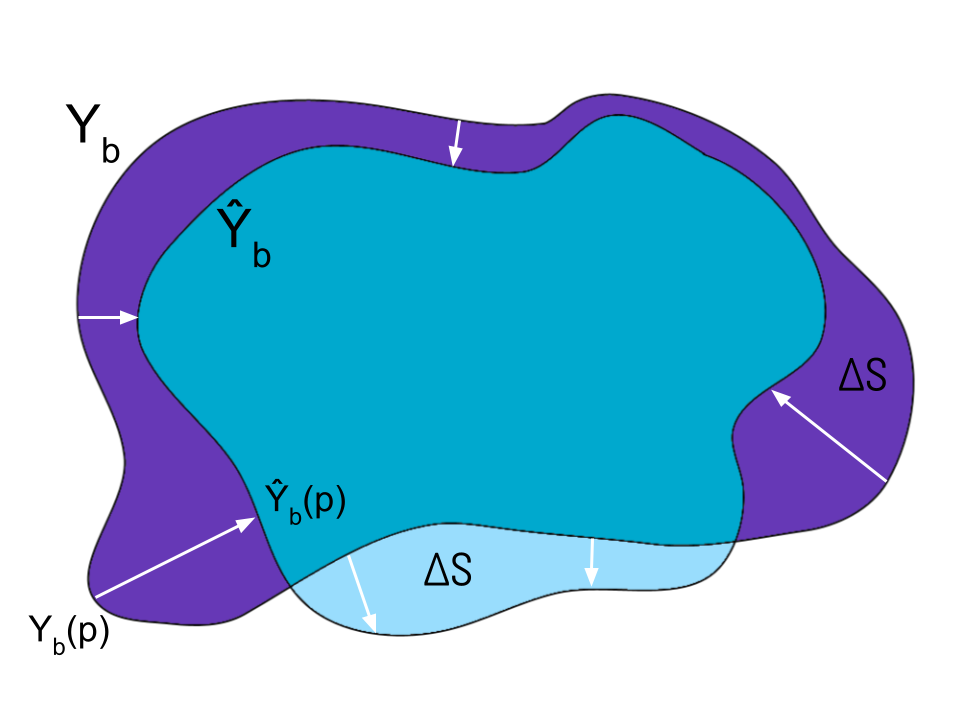
\includegraphics[width=0.5\textwidth]{images/BoundaryDiff.png}
    \caption[Boundary normals]{Schematic representation of the normals indicated as white arrows perpendicular to $Y_b$ at $Y_b(p)$ and its intersection at $\hat{Y}_b(p)$.}
    \label{BoundaryDiff}
\end{figure}
The loss proposed in \cite{Kervadec_2021} is inspired by graph-based optimization techniques \cite{boykov2006integral} and attempts to approach
\begin{equation}
    Dist(Y_b,\hat{Y}_b)=\int_{Y_b}||Y_b(p)-\hat{Y}_b(p)||^2 dp
    \label{eqn:boundary_diff}
\end{equation}
with
\begin{equation}
    Dist(Y_b,\hat{Y}_b)\approx 2\int_{\Delta S}D_y(q)dq
\end{equation}
where $Y_b(p)$ and $\hat{Y}_b(p)$ denote two corresponding points on the boundary connected by the normal to $Y_b$ at $p$ and its intersection $\hat{Y}_b(p)$. See \figref{BoundaryDiff}. As the expression \ref{eqn:boundary_diff} cannot be directly used for a loss due to local differential computations of the normal \cite{Kervadec_2021}, it can be approximated using the distance transform $D_y(q)$ where $q$ refers to any pixel on the ground truth $y$. The distance transforms $D_y(q)$, therefore, calculates the distance from $q$ to the closest point on the boundary $Y_b$.

The final loss is then calculated based on a level set representation \footnote{A level set representation is a method of representing objects and boundaries in a computer simulation or image processing using a level set function. The level set function assigns a numerical value to each point in a given space, such as an image or a three-dimensional model. Points inside or on the boundary have one value, while points outside the object have another. The points where the value of the function changes from one to another are called level sets. They are the contours of the object or the boundary.} $\varphi_y(q)$ which is calculated from the distance transform $D_y(q)$ as:
\begin{equation}
    \varphi_y(q)
    \begin{cases}
        -D_y(q) & \text{if }q\in y \\
        D_y(q)  & \text{otherwise}
    \end{cases}
    \label{eqn:varphi}
\end{equation}

\begin{figure}[H]%[htbp]
    \centering
    \subfigure[]{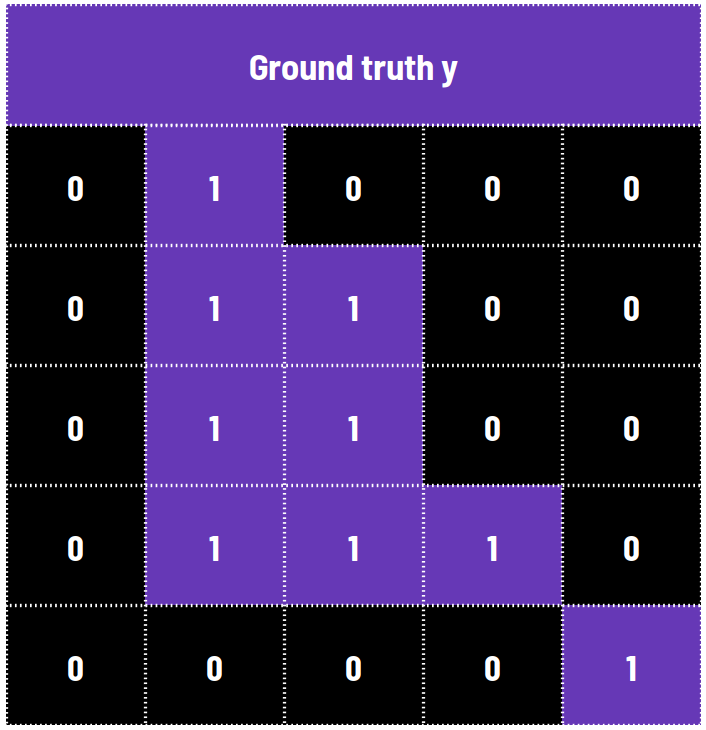
\includegraphics[width=\imgWidthThree]{images/varphi_q_1.png}}
    \subfigure[]{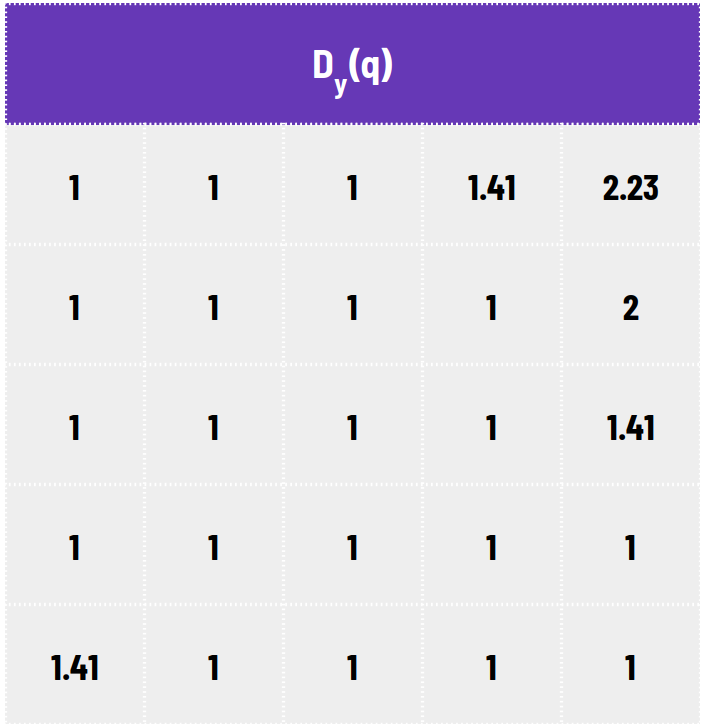
\includegraphics[width=\imgWidthThree]{images/varphi_q_2.png}}
    \subfigure[]{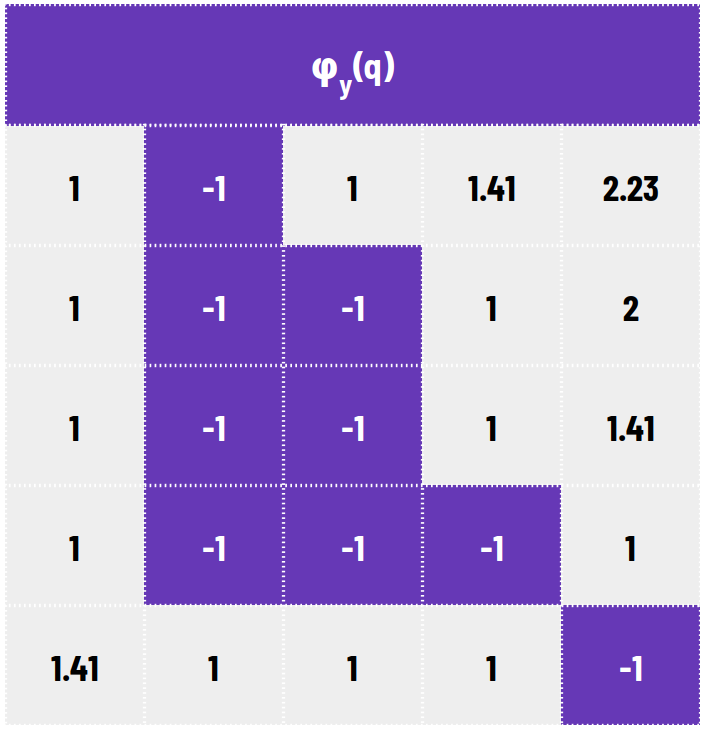
\includegraphics[width=\imgWidthThree]{images/varphi_q_3.png}}
    \caption[Calculation of $\varphi_y(q)$]{Example calculation of $\varphi_y(q)$ (c) from $y$ (a) with equation $\ref{eqn:varphi}$. Image (b) depicts the distance transform $D_y(q)$.}
    \label{varphi_q}
\end{figure}
which then leads to
\begin{equation}
    Dist(Y_b,\hat{Y}_b)=\int \varphi_y(q)\hat{y} dq -\int \varphi_y(q)y dq=BL
\end{equation}
which has the major advantage that the level set function $\varphi_y(q)$ can be precomputed from the ground truth as it does not change during training.
\begin{figure}[H]%[htbp]
    \centering
    \subfigure[]{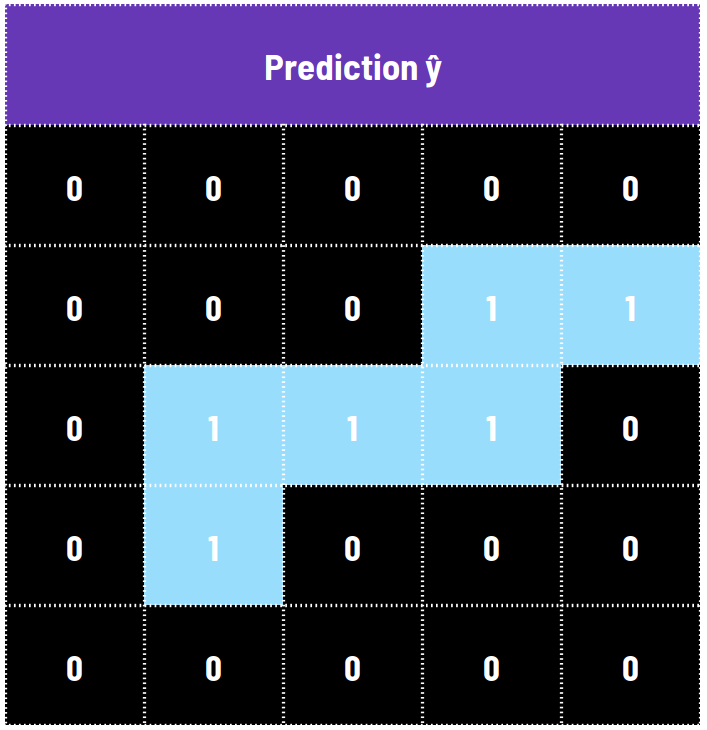
\includegraphics[width=\imgWidthFour]{images/boundary_final_1.png}}
    \subfigure[]{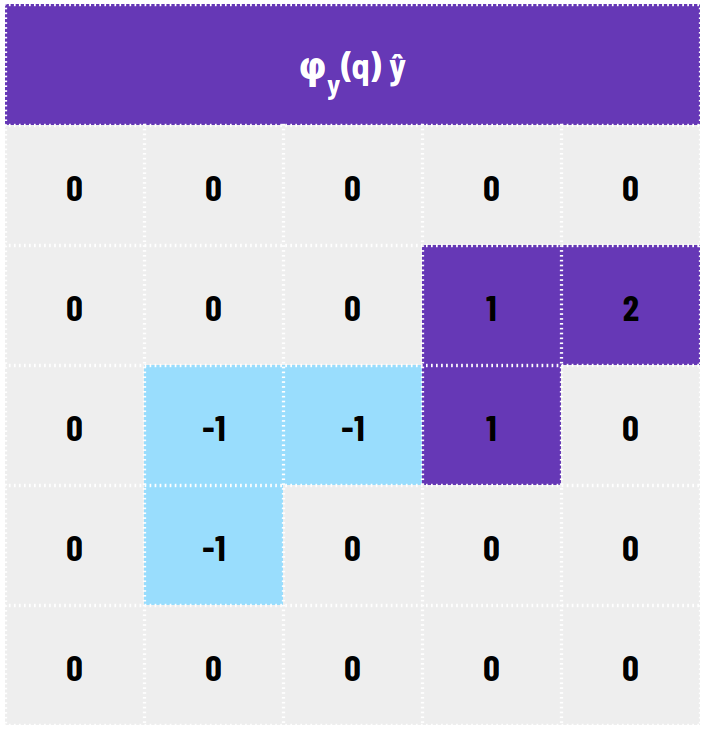
\includegraphics[width=\imgWidthFour]{images/boundary_final_2.png}}
    \subfigure[]{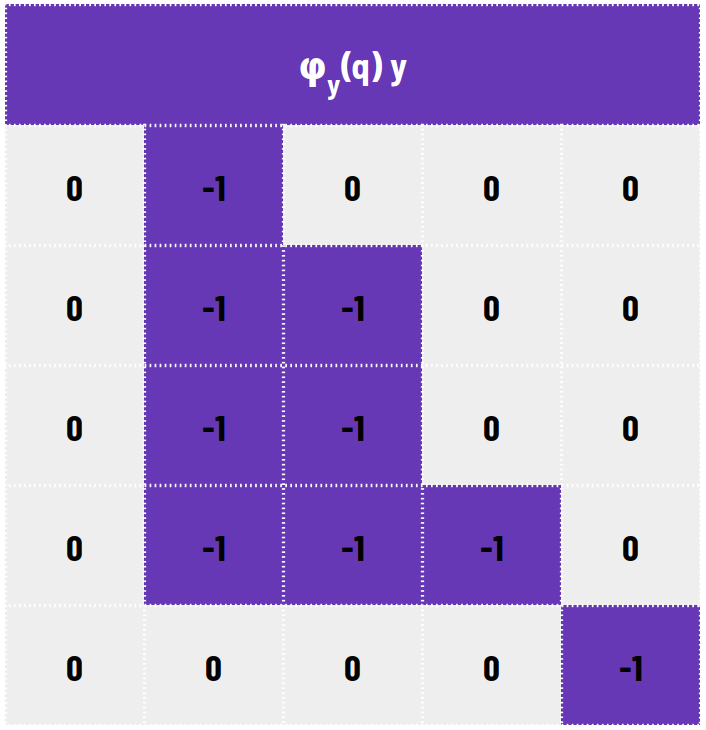
\includegraphics[width=\imgWidthFour]{images/boundary_final_3.png}}
    \subfigure[]{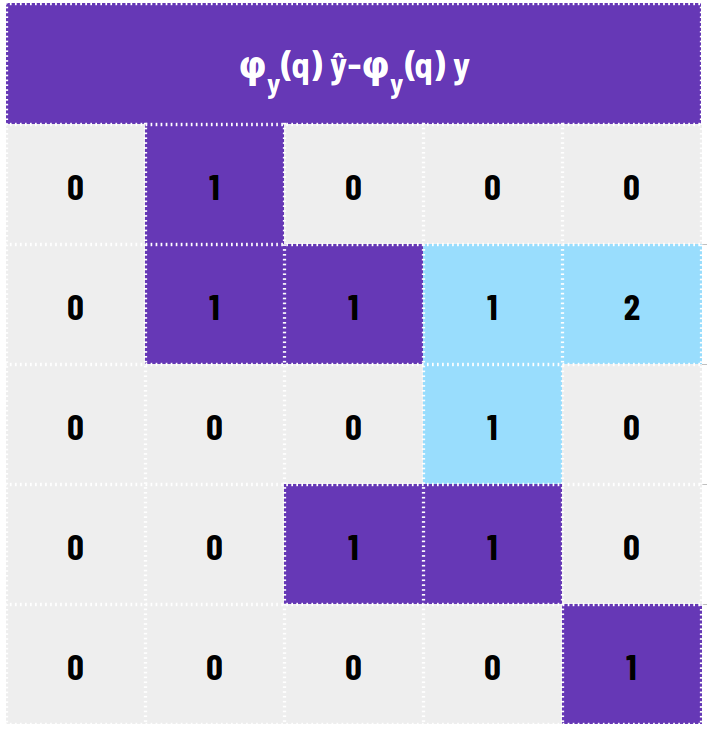
\includegraphics[width=\imgWidthFour]{images/boundary_final_4.png}}
    \caption[Final calculation of \ac{BL}]{Final calculation of \ac{BL} by precomputing the level set representation $\varphi_y(q)$ from the ground truth $y$ and multiplying it with the prediction $\hat{y}$ (b) and with the ground truth $y$ (c). To obtain the final boundary loss, the integrals $\int \varphi_y(q)\hat{y} dq$ and $\int \varphi_y(q)y dq$ are subtracted from each other (d).}
    \label{boundary_final}
\end{figure}

\subsection{Segmentation Metrics}
\label{subsec:segmentation_metrics}
Evaluating the performance of semantic segmentation models is critical to developing and optimizing practical algorithms for image understanding tasks. To assess the quality of a model's predictions, it is essential to utilize an appropriate measure to quantify the performance of the segmentation results. In this section, a variety of segmentation metrics commonly employed in classification tasks are explored. These metrics are the basis for comparing different models, understanding their strengths and weaknesses, and guiding further improvements. The following subsections will discuss each metric's underlying concepts, mathematical formulations, and practical applications, focusing on their relevance to semantic segmentation tasks.
\subsubsection*{Confusion Matrix}
\label{subsubsec:confusion_matrix}
Several of the following metrics use parts of the confusion matrix, a table used to describe the performance of a classification algorithm. The confusion matrix displays the number of correct and incorrect predictions made by the classifier. For semantic segmentation, the performance of each $\hat{y}\in \hat{Y}$ can be represented as a confusion matrix that summarizes all pixels within $\hat{y}$ as correct or incorrectly labeled. In the following, the rows of the confusion matrix represent the predicted class labels, while the columns represent the true (actual) class labels. The first cell in the first row represents the count of correctly classified as positive predictions.
In contrast, the second cell of the first row indicates the count of incorrectly classified as positive. The first cell in the second row represents the count of predictions incorrectly classified as negative, while the second cell correctly classified samples as negative. Even if confusion matrices exist for multi-class classification tasks, this work examines the binary case, which can be extended for multi-class classification. The confusion matrix for a binary classification problem has the following structure:
\begin{table}[H]
    \centering
    \begin{tabular}{c|c|c|}
        \cline{2-3}
                                                                                                                                           &
        \cellcolor[HTML]{000000}{\color[HTML]{FFFFFF} \begin{tabular}[c]{@{}c@{}}Actual \\ Positive\end{tabular}}                          &
        \cellcolor[HTML]{000000}{\color[HTML]{FFFFFF} \begin{tabular}[c]{@{}c@{}}Actual \\ Negative\end{tabular}}                            \\ \hline
        \multicolumn{1}{|c|}{\cellcolor[HTML]{000000}{\color[HTML]{FFFFFF} \begin{tabular}[c]{@{}c@{}}Predicted \\ Positive\end{tabular}}} &
        \cellcolor[HTML]{00A9CE}{\color[HTML]{FFFFFF} True Positive}                                                                       &
        \cellcolor[HTML]{99DDFD}{\color[HTML]{FFFFFF} False Positve}                                                                         \\ \hline
        \multicolumn{1}{|c|}{\cellcolor[HTML]{000000}{\color[HTML]{FFFFFF} \begin{tabular}[c]{@{}c@{}}Predicted \\ Negative\end{tabular}}} &
        \cellcolor[HTML]{6638B6}{\color[HTML]{FFFFFF} False Negative}                                                                      &
        \cellcolor[HTML]{9B7DD4}{\color[HTML]{FFFFFF} True Negative}                                                                         \\ \hline
    \end{tabular}
    \caption[Confusion matrix]{Structure of binary confusion matrix where the rows represent the predicted class labels while the cells represent the actual class. Each cell in the matrix represents the count of predictions where the true class is the column label, and the predicted class is the row label.}\label{tab:confusion_matrix}
\end{table}
Related to semantic segmentation, the values within the cells represent numbers of pixels described as follows:
\begin{itemize}[noitemsep]
    \item True Positive (TP): Number of correctly predicted pixels of the positive class
    \item False Positive (FP): Number of incorrectly predicted pixels of the positive class
    \item False Negative (FN): Number of incorrectly predicted pixels of the negative class
    \item True Negative (TN): Number of correctly predicted pixels of the negative class
\end{itemize}



\begin{figure}[H]%[htbp]
    \centering
    \subfigure[Output label]{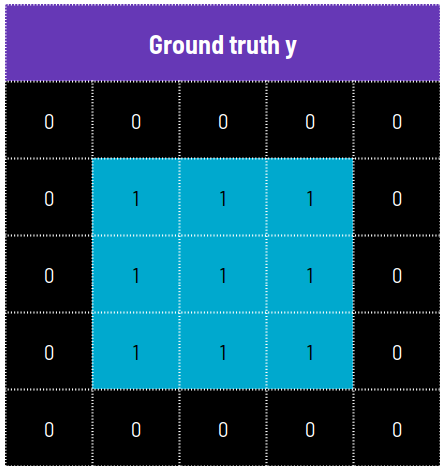
\includegraphics[width=\imgWidthTwo]{images/metrics_cm_gt.png}}
    \subfigure[Color coded prediction ]{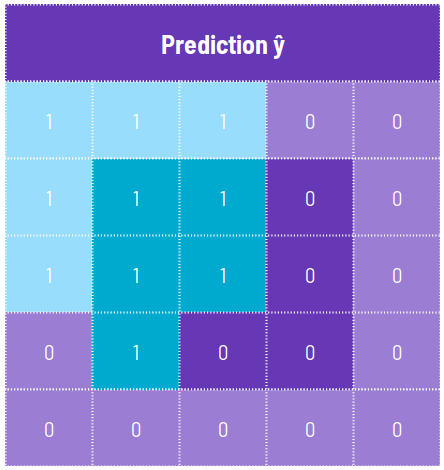
\includegraphics[width=\imgWidthTwo]{images/metrics_cm_yhat.png}}
    \caption[Output label and color-coded true/false positive/negative prediction]{Output label (a) and example of a 25-pixel visualization where each pixel is color-coded to indicate a \textbf{\textcolor{rwucyan}{True Positive}}, \textbf{\textcolor{rwucyanlight}{False Positive}}, \textbf{\textcolor{rwuviolet}{False Negative}} and \textbf{\textcolor{rwuvioletlight}{True Negative}} prediction (b) resulting in a confusion matrix of $\begin{bmatrix}5&5\\4&11\end{bmatrix}$.}
    \label{confusion_matrix_example}
\end{figure}
The following sections will describe some common metrics derived from the confusion matrix.

\subsubsection*{Precision (PPV), Recall (TPR)}
\label{subsubsec:precision_and_recall}
Precision and recall, also known as \ac{PPV} and \ac{TPR} are complementary metrics used to evaluate the performance of a classification task. The difference is that precision focuses on the number of false positives in addition to the true positives, while recall focuses on false negatives additionally to true positives.

The formal definition of precision and recall is as follows:
\begin{equation}
    \text{Precision}=\frac{TP}{TP+FP}
\end{equation}
\begin{equation}
    \text{Recall}=\frac{TP}{TP+FN}
\end{equation}
Intuitively, the perfect precision would have no false positives leading to a score of 1, while the perfect recall would have no false negatives, also leading to a score of 1. It is important to note that precision and recall are particularly relevant for the positive or foreground class in the context of semantic segmentation. \figref{precision_recall_metrics} illustrates two cases: one with high precision and low recall and the other with low precision and high recall. Based on the specific requirements and priorities of the segmentation task, a user might prefer one case over the other.

\begin{figure}[H]%[htbp]
    \centering
    \subfigure[High precision low recall]{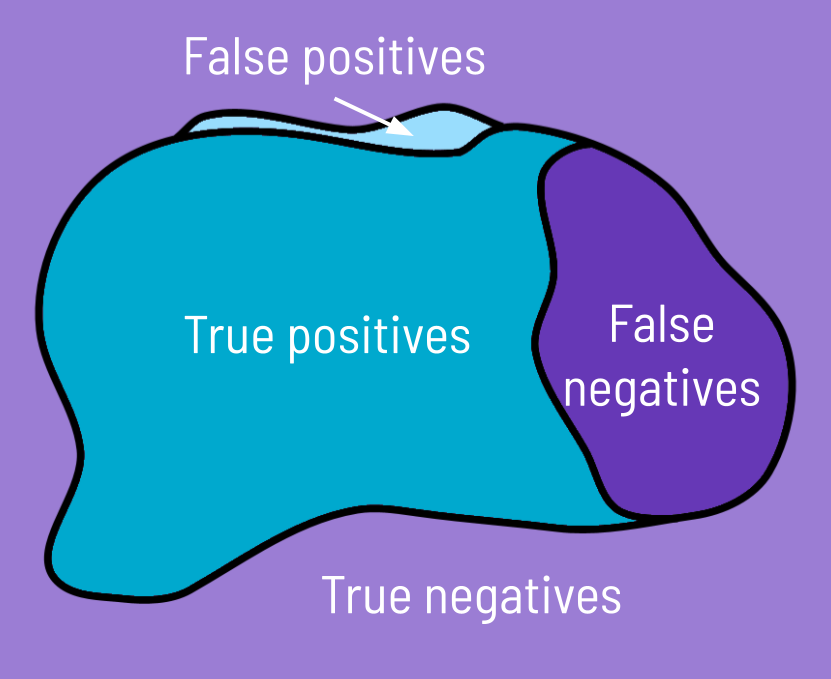
\includegraphics[width=\imgWidthTwo]{images/High_precision_low_recall_prototype.png}}
    \subfigure[Low precision high recall]{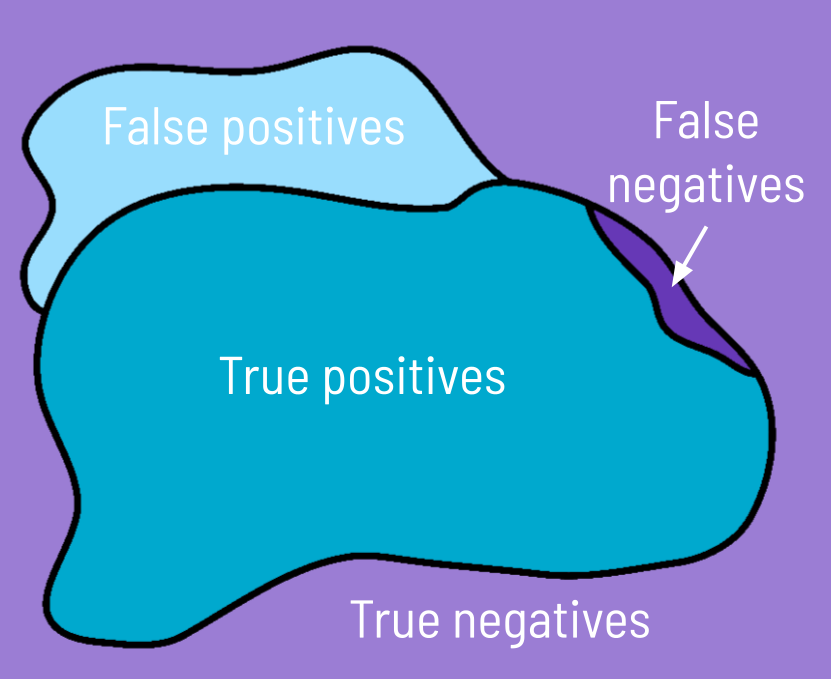
\includegraphics[width=\imgWidthTwo]{images/Low_precision_high_recall.png}}
    \caption[Precision and Recall]{Image (a) depicts a situation with very high precision. The false positives are very low. False negatives are high, which indicates a low recall. The situation in image (b) is the opposite, with a low precision and many false positives and a high recall with few false negatives.}
    \label{precision_recall_metrics}
\end{figure}

\subsubsection*{Specificity (TNR) and Negative Predictive Value (NPV)}
\label{subsubsec:specificity_and_negative_predictive_value}
Specificity, also known as \ac{TNR} and \ac{NPV}, are complementary metrics akin to precision and recall. However, these metrics emphasize true negatives instead of focusing on true positives. Specificity and \ac{NPV} are particularly useful in scenarios where the accurate identification of negative or background instances is crucial, such as in medical diagnostics \cite{Parikh2008-bd} or anomaly detection \cite{Henson2021}.

Specificity and negative predictive value are formally defined as follows:
\begin{equation}
    \text{Specificity}=\frac{TN}{TN+FP}
\end{equation}
\begin{equation}
    \text{Negative predictive value}=\frac{TN}{TN+FN}
\end{equation}
Intuitively, a perfect specificity score indicates no false positives, while a perfect \ac{NPV} implies no false negatives. In semantic segmentation, these metrics highlight the model's performance in correctly identifying negative or background classes.

\subsubsection*{Intersection over Union (IoU)}
\label{subsubsec:jaccard_index}
The \ac{IoU}, also known as the \ac{JI}, is a similarity measure used to compare two sample data objects. It is defined as the ratio of the intersection size to the union size \cite{Verma2020}.

Originally, the \ac{IoU} was described in set notation as:
\begin{equation}
    IOU=\frac{|A\cap B|}{|A \cup B|}=\frac{|A \cap B|}{|A|+|B|-|A\cap B|}
\end{equation}
where $A$ and $B$ represent two sets being compared.

In the context of confusion matrix components, the \ac{IoU} is defined as:
\begin{equation}
    IOU=\frac{TP}{TP+FP+FN}
\end{equation}
\subsubsection*{Dice Similarity Coefficient (DSC)}
\label{subsubsec:dice_similarity_coefficient}
The \ac{DSC}, also known as the \ac{SDI}, was originally defined in set notation to describe the similarity between two samples. It is a widely used measure for evaluating image segmentation algorithms, particularly within the medical field \cite{Carass2020-rj}. Given two sets, $A$ and $B$, the \ac{DSC} is defined as
\begin{equation}
    DSC=\frac{2|A\cap B|}{|A|+|B|}
\end{equation}
In terms of true positives (TP), false positives (FP), and false negatives (FN), the \ac{DSC} can be expressed as
\begin{equation}
    DSC=\frac{2\cdot TP}{2\cdot TP + FP + FN}
\end{equation}
Notably, true positives are counted twice in this measure, resulting in the \ac{DSC} having a higher value for the same number of correctly classified pixels than the \ac{IoU} metric.

\subsubsection*{Accuracy (Acc)}
\label{subsubsec:accuracy}
Accuracy measures the proportion of correctly classified pixels in an image defined as
\begin{equation}
    \text{Accuracy}=\frac{\text{Number of correctly classified pixels}}{\text{Total number of pixels}}
\end{equation}
where the number of correctly classified pixels also includes True Negative predictions. In terms of confusion matrix components, this metric can also be defined as
\begin{equation}
    \text{Accuracy}=\frac{TP+TN}{TP+TN+FP+FN}
\end{equation}

\subsubsection*{Multiclass Classification}
Previously, we discussed metric calculations for binary classification tasks involving only two classes. This concept can be extended to multi-class classification problems, where the output labels $y$ can be transformed from integers to one-hot-encoded format, as demonstrated in \figref{one_hot_encoded_mask}. With the predictions $\hat{y}$ provided in one-hot-encoded format, as shown in \figref{predictions_scores_softmax}, each class can be treated as a binary classification problem. To obtain a final metric score, we can calculate individual confusion matrices for each class and average the results. This approach is known as \texttt{macro averaging} and will be employed for this project. An alternative method, called \texttt{micro averaging}, involves calculating a single confusion matrix for all classes and using it to compute a single metric score. The following equations demonstrate the difference between these approaches for the \acf{IoU} metric.

\begin{equation}
    \text{Micro IoU} = \frac{\sum_{i=1}^{D} TP_i}{\sum_{i=1}^{D} (TP_i + FP_i + FN_i)}
    \label{eqn:micro_iou}
\end{equation}

\begin{equation}
    \text{Macro IoU} = \frac{1}{D} \sum_{i=1}^{D} \frac{TP_i}{(TP_i + FP_i + FN_i)}
    \label{eqn:macro_iou}
\end{equation}

Here, $D$ represents the number of classes, while $TP_i$, $FP_i$, and $FN_i$ denote the true positives, false positives, and false negatives for class $i$, respectively. \figref{multiclass_classification} further explores the differences between these approaches using an example that demonstrates metric calculation in an imbalanced situation.

\begin{figure}[H]
    \centering
    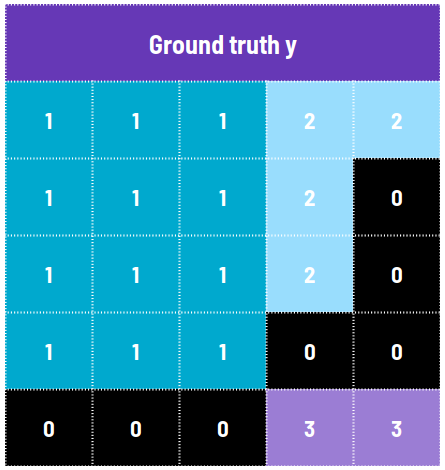
\includegraphics[width=\imgWidthTwo]{images/multiclass_example_y.png}
    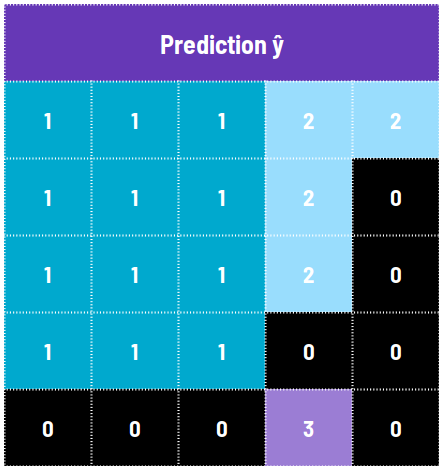
\includegraphics[width=\imgWidthTwo]{images/multiclass_example_yhat.png}
    \caption[Multiclass classification]{The \ac{IoU} using the micro average yields a value of $0.923$, whereas the macro \ac{IoU} average results in $0.843$. This significantly lower value for the 'macro' average primarily stems from the false negative prediction in pixel $\hat{Y}_{5,5}$, which leads to an \ac{IoU} score of $0.5$ for class three. According to equation \ref{eqn:macro_iou}, this prediction has a much larger impact on the overall result than in the micro \ac{IoU}, where the most prevalent class absorbs mispredictions for smaller classes. The prevalent class could be either the background or a foreground class with a considerably higher pixel count on average.}
    \label{multiclass_classification}
\end{figure}
\newpage

\subsection{Segmentation Architectures}
\label{subsec:segmentation_architectures}
The architecture employed in this project is derived from the U-Net, which is based on the \ac{EDA}. Introduced by \cite{DBLP:journals/corr/RonnebergerFB15} and illustrated in \figref{network_architecture}, the U-Net comprises two distinct paths: an encoding (contracting) path and a decoding (expanding) path, each composed of five layers. The encoding path incorporates pooling and convolutional operations along batch normalization and ReLU activation. It is responsible for capturing the context and reducing the spatial dimensions of the feature maps while increasing the number of channels. The decoding path upsamples the feature maps and concatenates them with the corresponding feature maps from the encoding path to provide high-resolution spatial information. After concatenation, the convolutions are applied to refine the feature maps. In this example, the final layer is a 1x1 convolution that maps the feature maps to the desired number of output classes resulting in a binary segmentation mask of shape 2x256x256 where each channel corresponds to one of the two classes in the binary segmentation.\cite{DBLP:journals/corr/RonnebergerFB15}
\begin{figure}[H]%[htbp]
    \centering
    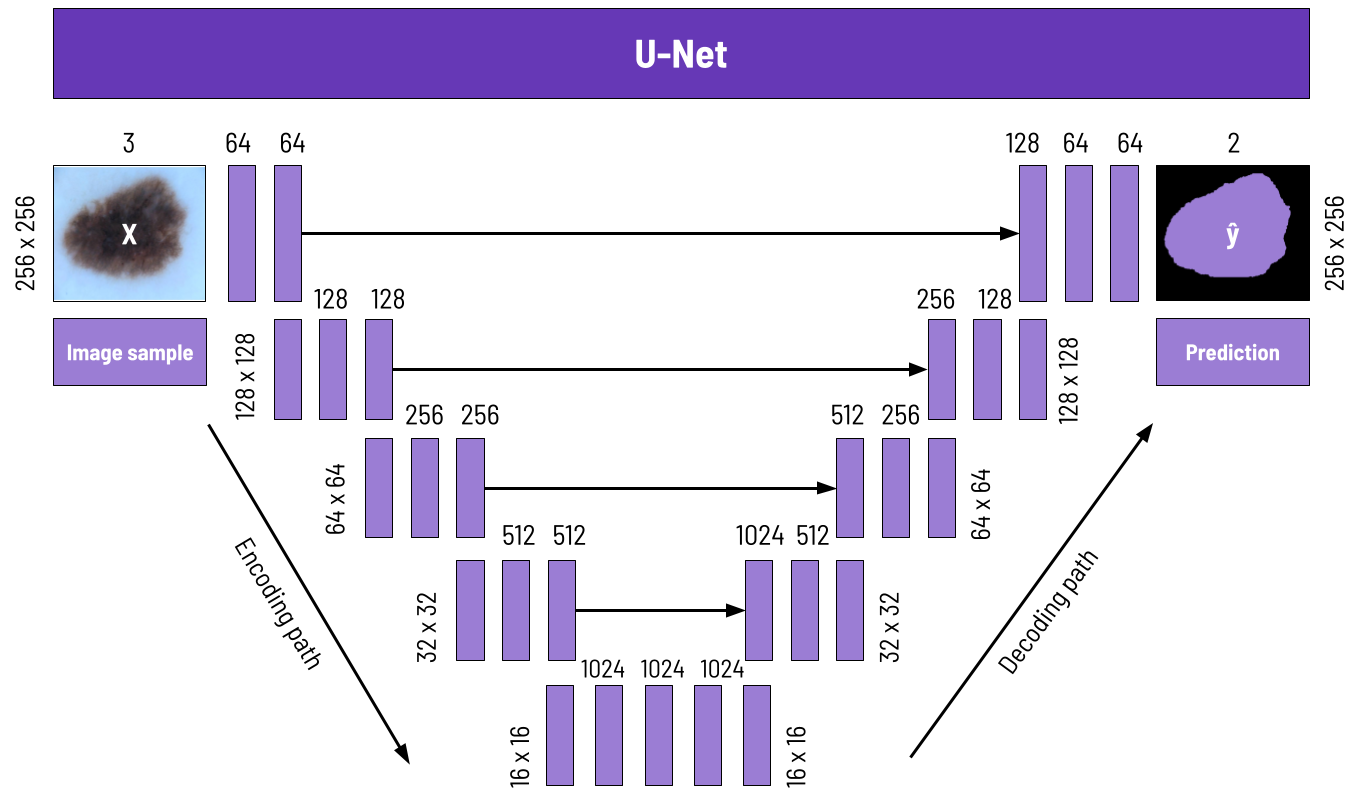
\includegraphics[width=\imgWidthXL]{images/NetworkArchitecture.png}
    \caption[U-Net]{U-Net model architecture proposed by \cite{DBLP:journals/corr/RonnebergerFB15}}
    \label{network_architecture}
\end{figure}
Besides the U-Net architecture, there is a wide variety of further models. \cite{doi:10.1080/08839514.2022.2032924} provides an excellent survey on deep learning architectures for semantic segmentation such as the \ac{SPP} \cite{doi:10.1080/08839514.2022.2032924} or the DeepLabv3+ Architecture\cite{Chen_2018_ECCV}.

\subsection{Segmentation Framework}
\label{subsec:segmentation_framework}
A segmentation framework follows a similar implementation as a standard deep learning framework presented as a model production cycle in \figref{model_production_cycle}, which entails configuration, preprocessing, training, validation, testing, and monitoring.
\begin{figure}[H]%[htbp]
    \centering
    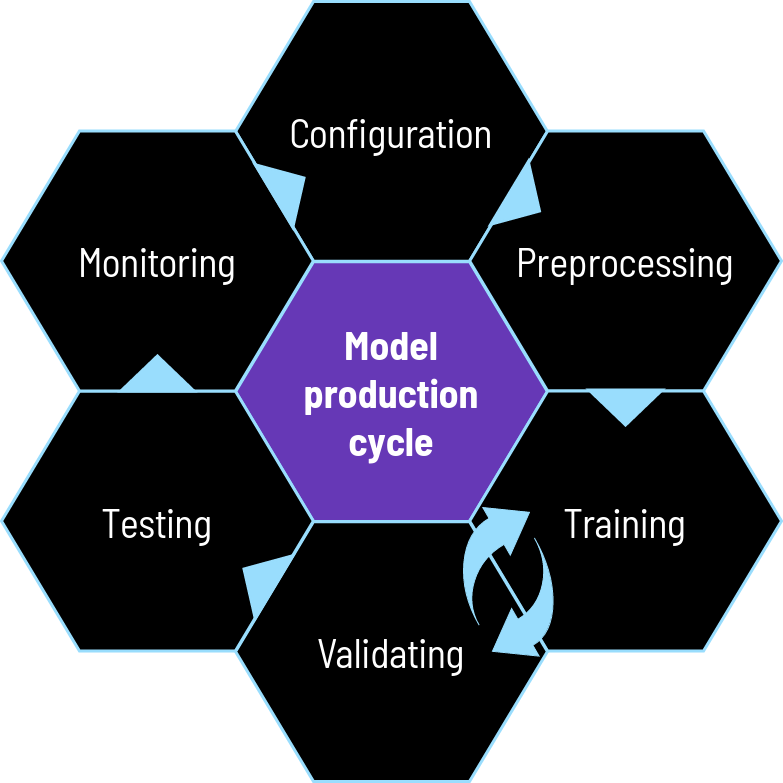
\includegraphics[width=\imgWidthM]{images/model_production_cycle.png}
    \caption[Experimental setup]{The model production cycle iteratively preprocesses, trains, validates, tests, and logs the results of each model using a specified configuration.}
    \label{model_production_cycle}
\end{figure}

\begin{enumerate}
    \item \textbf{\emph{Configuration}}: The configuration generally entails setting up the parameters used to train the model. There are various ways to efficiently search for hyperparameters, with the selection ultimately depending on several factors such as dataset size, computational resources, and chosen network architecture.
    \item \textbf{\emph{Preprocessing}}: The preprocessing step involves preparing the data for input into the model, which includes tasks such as data augmentation, normalization, and encoding of categorical features. This step ensures that the data is in a suitable training, validation, and testing format.
    \item \textbf{\emph{Training}}: The training process begins by iterating through all samples in the training set. For each input sample $x$, the model generates a prediction $\hat{y}$ and calculates a loss $l(\hat{y},y)$, which is used to adjust the models' weights via backpropagation which typically involves the optimization technique called gradient descent as discussed earlier. An optimizer such as the Adam optimizer can effectively determine an appropriate learning rate, also called step size for gradient descent, as it utilizes an adaptive learning rate for each parameter during the backpropagation process. Once this process is done for every sample, label pair within the training set, the model will be validated in the next step.
    \item \textbf{\emph{Validation}}: After completing the training steps, the validation step is carried out to assess the trained models' performance by generating predictions and testing them against the corresponding output labels from the validation set. No model parameter updates occur during this step. Once the validation steps are finished, the process begins anew with the training set. This cycle repeats until all epochs have been completed. Epochs refer to a single pass through the entire training dataset while training a model.
    \item \textbf{\emph{Testing}}: Finally, the testing step is performed on the test data, which has been previously separated from the entire dataset. The test data results are crucial for evaluating a model's performance, as they reveal its generalization capabilities on unseen data. Like the validation step, the model parameters remain unchanged during the test step.
    \item \textbf{\emph{Monitoring}}: Monitoring is a crucial part of the model production cycle as it helps track the progress of the training, validation, and testing processes, allowing for the detection of potential issues or improvements. This step includes logging performance metrics, visualizing model performance, and saving intermediate results for later analysis.
\end{enumerate}

\chapter{Literature Review}
\label{chap:literature_review}
The literature review presented in this chapter focuses specifically on the topic of custom loss functions, which is directly aligned with the primary focus of this thesis.  More specifically, this chapter provides a comprehensive overview of some of the most recent publications in this area, focusing on studies that, like this one, advocate for the use of loss function combinations or loss adjustments, to create a more precise learning signal than what standard loss functions can offer. While there is a wide range of literature available on loss functions and strategies for their enhancement, to the best of the authors' knowledge, no unified framework exists that systematically combines a predetermined set of prominent loss types in the manner suggested in this work.

For a more general review of semantic segmentation improvement strategies beyond the scope of this thesis, please refer to Appendix D: \squote{\nameref{chap:extended_literature_review}}.

\squote{Relax and focus on brain tumor segmentation} \cite{WANG2022102259} from 2022, presents a \ac{CNN} for fully automatic brain tumor segmentation. The authors of the paper acknowledge that one of the major challenges to accurately segmenting brain tumors is the great variation in location, size, structure, and morphological appearance, as well as the severe data imbalance that exist between brain tumors and non-tumor tissue, as well as among the different sub-regions within the brain tumor itself.

To address these challenges, the authors propose a hybrid model which incorporates several key components:
\begin{itemize}
    \item A dynamic combination of the \ac{FL} and \ac{DL} specifically designed to focus more on the smaller tumor sub-regions with more complex structures during the training process.
    \item A relaxation of boundary constraints for the inner tumor regions in a coarse-to-fine fashion to better recognize the overall structure of the brain tumor and the morphological relationship among different tumor sub-regions.
    \item A symmetric attention branch highlights the possible location of the brain tumor from the asymmetric features caused by the growth and expansion of abnormal brain tissues.
\end{itemize}

The authors of the paper claim that the proposed hybrid model can balance the learning capacity of the model between spatial details and high-level morphological features and can improve the overall segmentation performance of brain tumors. The model is validated on the publicly available brain tumor dataset from real patients called BRATS  2019 \cite{Menze2014-gj}. The experimental results show that their model improves the overall segmentation performance compared to the top approaches in the BRATS 2019 challenge.

\squote{PolyLoss: A Polynomial Expansion Perspective of Classification Loss Functions} \cite{leng2022polyloss} from 2022, presents a new framework named PolyLoss whose goal is to understand better and design loss functions for \acp{DNN}. The authors propose that commonly used classification loss functions such as \ac{CE} and \ac{FL} can be decomposed into a series of weighted polynomial functions. This framework allows for the importance of different polynomial bases to be adjusted depending on the target task and dataset. It demonstrates that better results can be achieved by adjusting these weights than with the commonly used loss functions. They also propose a simple and effective Poly-1 loss formulation that outperforms \ac{CE} and \ac{FL} on various tasks by only introducing one extra hyperparameter and adding one line of code.

\squote{Distribution-Aware Margin Calibration for Semantic Segmentation in Images} \cite{Yu2022} from 2022, describes a method to improve the performance of semantic segmentation models. The authors propose using a \squote{margin calibration} method, which can be used as a learning objective to improve the generalization of the IoU metric over the data distribution. The method theoretically ensures better segmentation performance in terms of \ac{IoU}. It has been evaluated on seven image datasets, showing substantial improvements in the IoU score over other learning objectives using deep segmentation models. In contrast, traditional loss functions, such as \ac{CE}, tend to have a poor indicator of model quality in semantic segmentation because the minimization of it does not guarantee a higher IoU score, which is more commonly used in semantic segmentation, specifically for sketching the contours of interest regions.

\squote{blob loss: instance imbalance aware loss functions for semantic segmentation} \cite{https://doi.org/10.48550/arxiv.2205.08209} from 2022, presents a new loss function called \squote{blob loss} for semantic segmentation tasks, which aims to improve instance-level detection metrics, such as F1 score and sensitivity.\footnote{$F1=\frac{2\cdot \text{Precision}\cdot \text{Recall}}{\text{Precision}+\text{Recall}}$} The authors argue that traditional loss functions, such as the \ac{DL}, do not take instance imbalance\footnote{Instance imbalance within a class occurs when there is a disproportionate number of instances with specific characteristics compared to others. Characteristics in this context could be different textures or morphological differences like size or shape \cite{https://doi.org/10.48550/arxiv.2205.08209}. For example, in a forest image dataset, there might be many trees with leaves but only a few without. Similarly, there could be significant and small tumors of the same class in medical imaging. This imbalance can lead to poor overall performance as models may struggle to identify less common instances accurately.} within a class into account, which can lead to sub-optimal results when the object of interest is highly heterogeneous. This is particularly relevant in medical applications, such as disease progression monitoring, where detecting small-scale lesions is critical. The proposed method is based on converting any loss function into a \squote{blob loss} by adding a term that represents the instance imbalance. This term is calculated as the ratio of the number of pixels belonging to the smaller instances to the number of pixels belonging to the more significant instances. The \squote{blob loss} is designed to work with semantic segmentation problems where the instances are connected components within a class.

The proposed method is evaluated on five complex 3D semantic segmentation tasks that feature pronounced instance heterogeneity in terms of texture and morphology. These tasks include multiple sclerosis lesions, liver tumors, and microscopy segmentation. The evaluation results showed that compared to the traditional soft \ac{DL}, the \squote{blob loss} achieved an average 2\% improvement for microscopy segmentation tasks considering F1 score and 5\% improvement for MS lesions.

The paper argues that the proposed \squote{blob loss} method addresses the issue of instance imbalance in semantic segmentation tasks, which is not adequately reflected in traditional loss functions such as \ac{DL}, and it can improve the performance of the model in detecting small scale lesions in medical applications.

\squote{Topology-Aware Segmentation Using Discrete Morse Theory} \cite{hu2021topologyaware} from 2021 proposes a new loss function incorporating topological information from the image segmentation task. The loss function is based on the concept of \ac{DMT}, a mathematical framework that uses the gradient vector field of the likelihood function to identify critical points and structures in the image. These structures, composed of 1D and 2D manifold pieces, reveal the topological information captured by the likelihood function. For more detailed information on \ac{DMT}, see \figref{morse_theory}.

\begin{figure}[H]%[htbp]
    \centering
    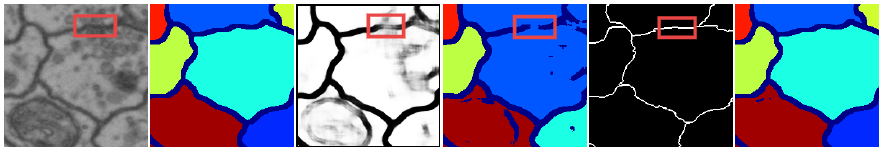
\includegraphics[width=\imgWidthXL]{images/morse_theory.png}
    \caption[\acf{DMT} predictions]{From left to right: Sample, Ground truth, Likelihood map, Baseline prediction, Critical structure with \ac{DMT} loss applied and final result. Image from \cite{hu2021topologyaware}}
    \label{morse_theory}
\end{figure}

The method identifies these critical structures, called Morse structures, as essential for topological accuracy. The loss function assigns a higher penalty to predictions that deviate from these structures. This way, the network is encouraged to produce predictions more consistent with the topological information.

The loss function is designed to correct false negatives, where a structure is a tree structure missed in the segmentation, and false positives, where a structure is a \squote{halluzination} of the model and should be removed. By enforcing higher penalties along the identified Morse structures, the network is forced to predict correctly near these topologically difficult locations and address the sampling bias issue \footnote{Sampling bias is a problem that occurs when the sample used in a study or survey is not representative of the population being studied, leading to inaccurate or misleading results \cite{10.1145/3457607}.}.

In summary, the new loss function proposed in the paper uses the concept of discrete Morse theory to identify global structures and critical points in the image. It incorporates this topological information into the training process by assigning a higher penalty to predictions that deviate from these structures. This approach improves the network's performance, especially near topologically challenging locations, and ensures that the network can produce segmentations with correct topology.

\squote{Tilted Cross Entropy {(TCE):} Promoting Fairness in Semantic Segmentation} \cite{DBLP:journals/corr/abs-2103-14051} from 2021, proposes a new loss function called \ac{TCE} for semantic segmentation in order to minimize performance disparities among target classes and promote fairness. The \ac{TCE} is inspired by the recently introduced \ac{TERM}\cite{li2020tilted} and is adapted to the semantic segmentation setting. The authors demonstrate through quantitative and qualitative performance analyses that the proposed \ac{TCE} can improve the low-performing classes of CityScapes \cite{cordts2016cityscapes} and ADE20k \cite{zhou2017scene} datasets and also results in improved overall fairness.

\squote{Rethinking the Dice Loss for Deep Learning Lesion Segmentation in Medical Images} \cite{9338261} from 2021 presents four limitations called \emph{Distance insensitivity}, \emph{Boundary insensitivity}, \emph{Region-size sensitivity} and \emph{Insensitivity to FP / FN weight}, for the \ac{DL} and how to overcome them. This section provides a detailed review of these limitations.

One significant weakness is the \squote{insensitivity to the distance} between non-overlapping regions, as highlighted by \cite{9338261}. This means that regardless of how far these regions are apart, the loss will remain constant even if, intuitively, a closer region should yield a lower loss. A computational example using the \ac{DL} is illustrated in \figref{dice_limit_1}.
\begin{figure}[H]%[htbp]
  \centering
  \subfigure[]{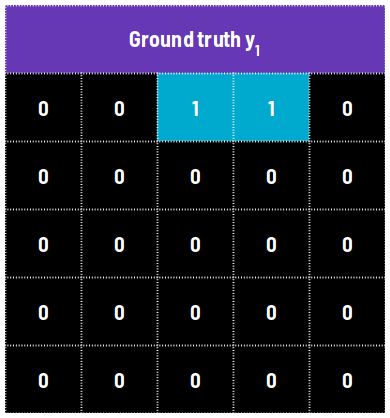
\includegraphics[width=\imgWidthFour]{images/dice_limit_1_1.png}}
  \subfigure[]{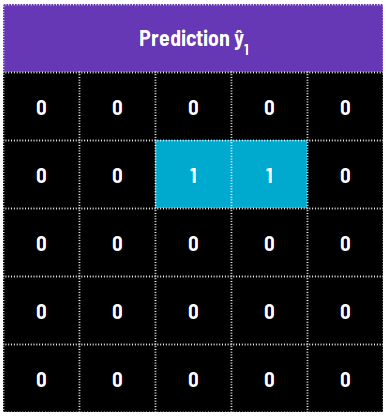
\includegraphics[width=\imgWidthFour]{images/dice_limit_1_2.png}}
  \subfigure[]{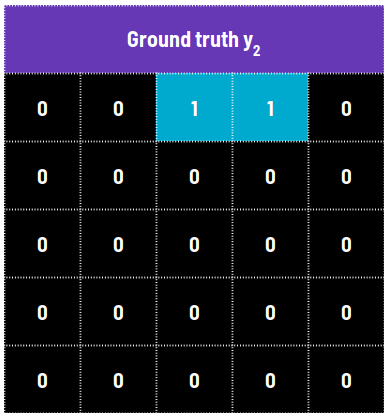
\includegraphics[width=\imgWidthFour]{images/dice_limit_1_3.png}}
  \subfigure[]{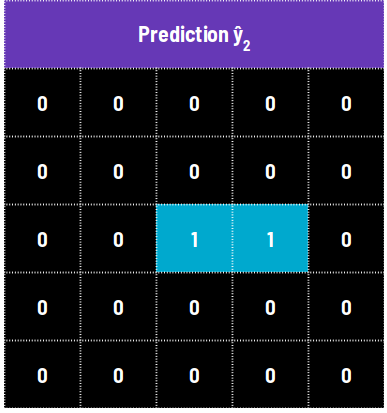
\includegraphics[width=\imgWidthFour]{images/dice_limit_1_4.png}}
  \caption[Distance insensitivity of \ac{DL}]{The images show the insensitivity to distance of the \ac{DL}. Image (a) and (c) depict the ground truths $y_1,y_2$, and image (b) and (d) the corresponding predictions $\hat{y}_1,\hat{y}_2$. It can be seen that even if $\hat{y}_1$ is closer to the ground truth than $\hat{y}_2$ the result for both predictions is the same with $DL_1=DL_2=1-\frac{2\cdot 0}{2\cdot 0 + 2 + 2}=1.0$.}
  \label{dice_limit_1}
\end{figure}
An additional limitation of the \ac{DL} is its \squote{insensitivity to boundaries}. The loss function cannot accurately account for the precise contours of segmented regions and fails to reflect how the overlap occurs if the number of true positives stays the same. See \figref{dice_limit_2} for a detailed illustration of the issue.
\begin{figure}[H]%[htbp]
  \centering
  \subfigure[]{\includegraphics[width=\imgWidthFour]{images/dice_limit_2_1.png}}
  \subfigure[]{\includegraphics[width=\imgWidthFour]{images/dice_limit_2_2.png}}
  \subfigure[]{\includegraphics[width=\imgWidthFour]{images/dice_limit_2_3.png}}
  \subfigure[]{\includegraphics[width=\imgWidthFour]{images/dice_limit_2_4.png}}
  \caption[Boundary insensitivity of \ac{DL}]{The images demonstrate the boundary insensitivity of the \ac{DL}. Image (a) and (c) depict the ground truths $y_1,y_2$, and image (b) and (d) the corresponding predictions $\hat{y}_1,\hat{y}_2$. Despite their visual differences, both overlaps yield an identical loss with $DL_1=DL_2=1-\frac{2\cdot 3}{2\cdot 3 + 2 + 3}= 0.5$.}
  \label{dice_limit_2}
\end{figure}
Another notable limitation of the \ac{DL} is its \squote{sensitivity to region size}. Consider a scenario where a large region needs to be predicted. If a single pixel is misclassified, the resulting loss is much lower than if a pixel is misclassified when predicting smaller regions. See \figref{dice_limit_3} for further illustration.
\begin{figure}[H]%[htbp]
  \centering
  \subfigure[]{\includegraphics[width=\imgWidthFour]{images/dice_limit_3_1.png}}
  \subfigure[]{\includegraphics[width=\imgWidthFour]{images/dice_limit_3_2.png}}
  \subfigure[]{\includegraphics[width=\imgWidthFour]{images/dice_limit_3_3.png}}
  \subfigure[]{\includegraphics[width=\imgWidthFour]{images/dice_limit_3_4.png}}
  \caption[Sensitivity towards small region of \ac{DL}]{The images demonstrate the sensitivity towards small regions. In images (a) and (b), the ground truth $y$ and prediction $\hat{y}$ have a misclassification of one pixel, resulting in a \ac{DL} of $DL_1=1-\frac{2\cdot 15}{2\cdot 15 + 0 + 1}\approx 0.03$. On the other hand, in the image (c) and (d), the misclassification occurs on a smaller region resulting in a higher \ac{DL} of $DL_2=1-\frac{2\cdot 3}{2\cdot 3 + 0 + 1}\approx 0.142$}
  \label{dice_limit_3}
\end{figure}
A further limitation of the \ac{DL}, described in \cite{9338261}, is its \squote{insensitivity to FP / FN weight}, or which can be a disadvantage since, depending on the task, researchers want to weigh false positives or false negatives differently. To illustrate this limitation, consider the example shown in \figref{dice_limit_4}.
\begin{figure}[H]%[htbp]
  \centering
  \subfigure[]{\includegraphics[width=\imgWidthFour]{images/dice_limit_4_1.png}}
  \subfigure[]{\includegraphics[width=\imgWidthFour]{images/dice_limit_4_2.png}}
  \subfigure[]{\includegraphics[width=\imgWidthFour]{images/dice_limit_4_3.png}}
  \subfigure[]{\includegraphics[width=\imgWidthFour]{images/dice_limit_4_4.png}}
  \caption[Insensitivity to FP / FN weight \ac{DL}]{The concept of insensitivity to the weight put on false negative and false positive predictions is demonstrated in this figure. The loss from (a) and (b) $DL_1 = 1-\frac{2*3}{2*3+1+0}\approx 0.142$ is the same as the loss from (c) and (d) $DL_2 = 1-\frac{2*3}{2*3+0+1}\approx 0.142$.}
  \label{dice_limit_4}
\end{figure}

\newpage
\chapter{Methodology}
\label{chap:methodology}
This chapter outlines the methodology that offers a unique framework for users to experiment with multiple loss functions, combining them and applying several merging strategies to output a final loss. The goal is to enable users to gain insights into the most suitable combination for their specific data. The chapter is organized into two sections. The \nameref{sec:limiting_factors} section expands upon the constraints of the \acf{DL} as mentioned earlier, incorporating additional limitations and summarizing them to lay the groundwork for the subsequent section. In section \nameref{sec:loss_merging}, a framework is introduced that facilitates combining and merging multiple loss functions to address the discussed limitations and enhance the performance compared to models trained with individual loss functions.

\begin{figure}[H]%[htbp]
  \centering
  \includegraphics[width=\imgWidthXL]{images/Pipeline_white_bg.png}
  \caption[Proposed segmentation framework]{Illustration of the proposed framework where individual losses originating from distribution, region, or boundary-based types are generated in each training iteration. These losses are combined and merged using various proposed strategies, resulting in a single, unified loss. This approach aims to enhance performance beyond that of baseline models, which are trained with just a single loss function.}
  \label{framework}
\end{figure}

\section{Limiting Factors}
\label{sec:limiting_factors}
This section extends the taxonomy introduced by \cite{9338261} for the \ac{DL}, addressing the following limitations for the six loss functions introduced in \secref{subsec:segmentation_objectives}.
\begin{enumerate}
  \item \textbf{Distance insensitivity:} As previously discussed in the context of the \acf{DL}, insensitivity to distances is a notable limitation for a range of loss functions. Among the functions covered in \secref{subsec:segmentation_objectives}, all distribution and region-based functions exhibit this limitation. For distribution-based functions, this limitation can be demonstrated analogously to what is shown for \ac{DL} in \figref{dice_limit_1}. However, this insensitivity does not constrain boundary-based loss functions that incorporate a distance transform in their calculations. See the corresponding row of table \ref{tab:limitation_quantitative_results} for quantitative analysis.
  \item \textbf{Boundary insensitivity:} This limitation, initially introduced in \chapref{chap:literature_review} for the \ac{DL}, is also pertinent to distribution and region-based loss functions. The two boundary-based loss functions, namely \ac{HL} and \ac{BL}, appear to be somewhat resilient to this limitation, although they are not completely aware of the entire shape. In instances where two predictions are compared - with the first matching the shape of the ground truth but located farther away than a second prediction that exhibits a different shape - the latter might yield a smaller loss, thereby providing possible misleading feedback. As demonstrated in table \ref{tab:limitation_quantitative_results}, distribution and region-based losses yield the same result.
  \item \textbf{Region-size sensitivity:} This sensitivity is associated with the issue of class imbalance and predominantly affects distribution and region-based loss functions. While initially introduced in the context of \ac{DL} in \chapref{chap:literature_review}, distribution-based loss functions are known to work best on data with equal distribution and thus are also affected by sensitivity to region size \cite{Jadon_2020} \cite{YEUNG2022102026} while boundary-based loss functions are not affected by this type of sensitivity. Table \ref{tab:limitation_quantitative_results} presents a quantitative analysis where distribution and region-based losses change substantially comparing $l_1$ with $l_2$ where the former represents one misclassified pixel on large regions while the latter stems from one misclassified pixel on small regions.
  \item \textbf{FP / FN weight insensitivity:} All loss functions, with the exception of the \acf{TL}, which is explicitly designed to address this issue, exhibit insensitivity to the weighting of false positives and false negatives. As highlighted in \secref{subsec:segmentation_metrics}, researchers may desire to manipulate high precision, low recall scenarios, or vice versa, depending on specific objectives. This manipulation can be achieved by manually adjusting the weights attributed to false positives or false negatives. On table \ref{tab:limitation_quantitative_results} we can see that the \ac{TL} is the only function sensitive to FP / FN weight.
  \item \textbf{Outlier sensitivity:} Outliers can be described as data points unusually distant from the overall pattern and deviate significantly from other observations. Outliers may arise for various reasons, such as errors in labeling or the presence of noise. In the context of loss functions discussed in \secref{subsec:segmentation_objectives}, it is essential to note that all loss functions can be sensitive to outliers. This sensitivity can disproportionately affect the model's total loss value during training. While it is generally difficult to ascertain which loss function is most affected by outliers, it is observed that boundary-based loss functions are more impacted when the mislabeled pixels are further from the region of interest. Conversely, region-based loss functions are influenced equally by pixels closer to or further from the region of interest. While many techniques exist, such as data augmentation and regularization, which can mitigate the impact of outliers and enhance the model's performance. For a more comprehensive understanding of this subject, please refer to \cite{Cho_2023_WACV}, \cite{DBLP:journals/corr/abs-1802-09129}, \cite{bevandi2019simultaneous}.
  \item \textbf{Computational complexity:} Boundary-based loss functions are known to be computationally expensive since they involve distance calculations between sets of points, which are much more complex and time-consuming compared to other loss functions \cite{Kervadec_2021}. To reduce the complexity of the \ac{HL} function, the one-sided version $HL_{os}$ can be used instead, as defined in \ref{eq:one_sided_hd}, to reduce the effort of the distance transform $D_y(i,j)$, as defined in \ref{eqn:distance_transform_y}, for the ground truth only. Since $D_y(i,j)$ does not change during training, it can be pre-calculated for all output labels $Y$ whenever the model is initialized. Similarly, the \ac{BL} function presented in \secref{subsec:segmentation_objectives} also requires the distance transformation to be pre-calculated, which can cause a bottleneck, especially for high-resolution images. To further reduce computational complexity, a subsampling method can use only a subset of points instead of all the pixels in the image.
  \item \textbf{Manual parameter tuning:} Manual hyperparameter tuning can be a limiting factor for loss functions. Hyperparameter search can be time-consuming, especially when dealing with large datasets or complex architectures. It may also require domain expertise related to the dataset or the clinical operation, as discussed in \secref{subsec:tversky}. Additionally, hyperparameter search only sometimes guarantees to find the best solution since it relies on the intuition or experience of the user. To improve manual tuning and increase the likelihood of finding an optimal set of values, techniques such as grid search \cite{9504761}, random search \cite{10.5555/2188385.2188395}, Bayesian optimization \cite{WU201926}, or evolutionary algorithms \cite{DBLP:journals/corr/abs-2105-09821} can be used. These techniques automate the hyperparameter search process and can save time and resources.
\end{enumerate}
The following table \ref{tab:limitation_quantitative_results} presents the quantitative results for limitations 1 through 4 confirming each statement from above. Each loss column displays two results, $l_1$ and $l_2$, which correspond to specific combinations of $y$ and $\hat{y}$, as previously discussed in the context of \acf{DL} in \chapref{chap:literature_review}. The results that are underlined indicate scenarios that are either not affected or less affected by the corresponding limitation.

% Please add the following required packages to your document preamble:
% \usepackage{graphicx}
% \usepackage[table,xcdraw]{xcolor}
% If you use beamer only pass "xcolor=table" option, i.e. \documentclass[xcolor=table]{beamer}
% \usepackage[normalem]{ulem}
% \useunder{\uline}{\ul}{}
\begin{table}[H]
  \centering
  \resizebox{\textwidth}{!}{%
  \begin{tabular}{l|cccc|cccc|cccc|l}
  \cline{2-13}
   &
    \multicolumn{4}{c|}{\cellcolor[HTML]{6638B6}{\color[HTML]{FFFFFF} \textbf{DB}}} &
    \multicolumn{4}{c|}{\cellcolor[HTML]{00A9CE}{\color[HTML]{FFFFFF} \textbf{RB}}} &
    \multicolumn{4}{c|}{\cellcolor[HTML]{99DDFD}{\color[HTML]{FFFFFF} \textbf{BB}}} &
     \\ \cline{2-13}
   &
    \multicolumn{2}{c|}{\cellcolor[HTML]{000000}{\color[HTML]{FFFFFF} CE}} &
    \multicolumn{2}{c|}{\cellcolor[HTML]{000000}{\color[HTML]{FFFFFF} FL}} &
    \multicolumn{2}{c|}{\cellcolor[HTML]{000000}{\color[HTML]{FFFFFF} DL}} &
    \multicolumn{2}{c|}{\cellcolor[HTML]{000000}{\color[HTML]{FFFFFF} TL}} &
    \multicolumn{2}{c|}{\cellcolor[HTML]{000000}{\color[HTML]{FFFFFF} BL}} &
    \multicolumn{2}{c|}{\cellcolor[HTML]{000000}{\color[HTML]{FFFFFF} HL}} &
    \multicolumn{1}{c}{} \\ \cline{2-14} 
   &
    \multicolumn{1}{c|}{$l_1$} &
    \multicolumn{1}{c|}{$l_2$} &
    \multicolumn{1}{c|}{$l_1$} &
    $l_2$ &
    \multicolumn{1}{c|}{$l_1$} &
    \multicolumn{1}{c|}{$l_2$} &
    \multicolumn{1}{c|}{$l_1$} &
    $l_2$ &
    \multicolumn{1}{c|}{$l_1$} &
    \multicolumn{1}{c|}{$l_2$} &
    \multicolumn{1}{c|}{$l_1$} &
    $l_2$ &
    \multicolumn{1}{c|}{Reference} \\ \hline
  \multicolumn{1}{|l|}{\cellcolor[HTML]{9B7DD4}{\color[HTML]{FFFFFF} Distance Insensitivity}} &
    \multicolumn{1}{c|}{8.16} &
    \multicolumn{1}{c|}{8.16} &
    \multicolumn{1}{c|}{8.15} &
    8.15 &
    \multicolumn{1}{c|}{1.00} &
    \multicolumn{1}{c|}{1.00} &
    \multicolumn{1}{c|}{\cellcolor[HTML]{FFFFFF}0.67} &
    \cellcolor[HTML]{FFFFFF}0.67 &
    \multicolumn{1}{c|}{\cellcolor[HTML]{FFFFFF}{\ul 0.04}} &
    \multicolumn{1}{c|}{\cellcolor[HTML]{FFFFFF}{\ul 0.08}} &
    \multicolumn{1}{c|}{\cellcolor[HTML]{FFFFFF}{\ul 0.15}} &
    \cellcolor[HTML]{FFFFFF}{\ul 0.39} &
    \multicolumn{1}{l|}{\figref{dice_limit_1}} \\ \hline
  \multicolumn{1}{|l|}{\cellcolor[HTML]{9B7DD4}{\color[HTML]{FFFFFF} Boundary insensitivity}} &
    \multicolumn{1}{c|}{6.36} &
    \multicolumn{1}{c|}{6.36} &
    \multicolumn{1}{c|}{6.35} &
    6.35 &
    \multicolumn{1}{c|}{0.40} &
    \multicolumn{1}{c|}{0.40} &
    \multicolumn{1}{c|}{\cellcolor[HTML]{FFFFFF}0.33} &
    \cellcolor[HTML]{FFFFFF}0.33 &
    \multicolumn{1}{c|}{\cellcolor[HTML]{FFFFFF}0.04} &
    \multicolumn{1}{c|}{\cellcolor[HTML]{FFFFFF}0.04} &
    \multicolumn{1}{c|}{\cellcolor[HTML]{FFFFFF}{\ul 0.15}} &
    \cellcolor[HTML]{FFFFFF}{\ul 0.18} &
    \multicolumn{1}{l|}{\figref{dice_limit_2}} \\ \hline
  \multicolumn{1}{|l|}{\cellcolor[HTML]{9B7DD4}{\color[HTML]{FFFFFF} Region-size sensitivity}} &
    \multicolumn{1}{c|}{0.32} &
    \multicolumn{1}{c|}{1.68} &
    \multicolumn{1}{c|}{0.32} &
    1.68 &
    \multicolumn{1}{c|}{0.03} &
    \multicolumn{1}{c|}{0.14} &
    \multicolumn{1}{c|}{\cellcolor[HTML]{FFFFFF}0.04} &
    \cellcolor[HTML]{FFFFFF}0.15 &
    \multicolumn{1}{c|}{\cellcolor[HTML]{FFFFFF}{\ul 0.01}} &
    \multicolumn{1}{c|}{\cellcolor[HTML]{FFFFFF}{\ul 0.01}} &
    \multicolumn{1}{c|}{\cellcolor[HTML]{FFFFFF}{\ul 0.04}} &
    \cellcolor[HTML]{FFFFFF}{\ul 0.04} &
    \multicolumn{1}{l|}{\figref{dice_limit_3}} \\ \hline
  \multicolumn{1}{|l|}{\cellcolor[HTML]{9B7DD4}{\color[HTML]{FFFFFF} FP / FN weight insensitivity}} &
    \multicolumn{1}{c|}{1.68} &
    \multicolumn{1}{c|}{1.68} &
    \multicolumn{1}{c|}{1.68} &
    1.68 &
    \multicolumn{1}{c|}{0.14} &
    \multicolumn{1}{c|}{0.14} &
    \multicolumn{1}{c|}{\cellcolor[HTML]{FFFFFF}{\ul 0.07}} &
    \cellcolor[HTML]{FFFFFF}{\ul 0.14} &
    \multicolumn{1}{c|}{\cellcolor[HTML]{FFFFFF}0.01} &
    \multicolumn{1}{c|}{\cellcolor[HTML]{FFFFFF}0.01} &
    \multicolumn{1}{c|}{\cellcolor[HTML]{FFFFFF}0.04} &
    \cellcolor[HTML]{FFFFFF}0.04 &
    \multicolumn{1}{l|}{\figref{dice_limit_4}} \\ \hline
  \end{tabular}%
  }
  \caption{Results demonstrating limitation no. 1 to 4 for six loss functions quantitatively.}
  \label{tab:limitation_quantitative_results}
  \end{table}

\subsection{Summary}
Table \ref{tab:limiting_factors} summarizes the impact of each limiting factor on the six loss functions presented. It reveals that \ac{HL} and \ac{BL} are less affected by distance insensitivity, boundary insensitivity, and region-size sensitivity compared to the other loss functions. However, boundary-based loss functions have drawbacks, such as computational complexity, instability, and complex implementations.

Finding a single loss function that entirely circumvents all limitations is challenging. Nonetheless, the subsequent chapter explores a set of combinations of loss functions and merging techniques to leverage the individual strengths of each loss function to generate a more precise learning signal, thereby enhancing performance. This improvement can be important in various fields requiring a highly accurate segmentation performance, including distance measurements.

Although various implementations have attempted to address some of these limitations, such as the \ac{TL}, proposed by \cite{DBLP:journals/corr/SalehiEG17a}, which tackles the FP/FN weight insensitivity or the \ac{GDL} from \cite{Sudre_2017}, which is capable of handling region-size insensitivity there is an absence of a unified framework that systematically combines and analyzes a set of loss functions. To the best of the author's knowledge, such a unified, comprehensive approach is yet to be developed.
% Please add the following required packages to your document preamble:
% \usepackage{multirow}
% \usepackage{graphicx}
% \usepackage[table,xcdraw]{xcolor}
% If you use beamer only pass "xcolor=table" option, i.e. \documentclass[xcolor=table]{beamer}
\begin{table}[H]
  \centering
  \resizebox{\textwidth}{!}{%
  \begin{tabular}{cc|ccccccc|}
  \cline{3-9}
  {\color[HTML]{000000} } &
    {\color[HTML]{000000} } &
    \multicolumn{7}{c|}{\cellcolor[HTML]{000000}{\color[HTML]{FFFFFF} \textbf{Limiting factors}}} \\ \cline{2-9} 
  \multicolumn{1}{c|}{{\color[HTML]{000000} }} &
    \cellcolor[HTML]{9B7DD4}{\color[HTML]{000000} Loss} &
    \multicolumn{1}{c|}{\cellcolor[HTML]{9B7DD4}{\color[HTML]{FFFFFF} \begin{tabular}[c]{@{}c@{}}Distance\\ insensitivity\end{tabular}}} &
    \multicolumn{1}{c|}{\cellcolor[HTML]{9B7DD4}{\color[HTML]{FFFFFF} \begin{tabular}[c]{@{}c@{}}Boundary \\ insensitivity\end{tabular}}} &
    \multicolumn{1}{c|}{\cellcolor[HTML]{9B7DD4}{\color[HTML]{FFFFFF} \begin{tabular}[c]{@{}c@{}}Region-size\\ sensitivity\end{tabular}}} &
    \multicolumn{1}{c|}{\cellcolor[HTML]{9B7DD4}{\color[HTML]{FFFFFF} \begin{tabular}[c]{@{}c@{}}FP / FN weight\\ insensitivity\end{tabular}}} &
    \multicolumn{1}{c|}{\cellcolor[HTML]{9B7DD4}{\color[HTML]{FFFFFF} \begin{tabular}[c]{@{}c@{}}Outlier\\ sensitivity\end{tabular}}} &
    \multicolumn{1}{c|}{\cellcolor[HTML]{9B7DD4}{\color[HTML]{FFFFFF} \begin{tabular}[c]{@{}c@{}}Cumputational\\ complexity\end{tabular}}} &
    \cellcolor[HTML]{9B7DD4}{\color[HTML]{FFFFFF} \begin{tabular}[c]{@{}c@{}}Manual parameter\\ tuning\end{tabular}} \\ \cline{2-9} 
  \multicolumn{1}{c|}{\cellcolor[HTML]{6638B6}{\color[HTML]{FFFFFF} }} &
    \cellcolor[HTML]{000000}{\color[HTML]{FFFFFF} CE} &
    \multicolumn{1}{c|}{{\color[HTML]{000000} +++}} &
    \multicolumn{1}{c|}{{\color[HTML]{000000} +++}} &
    \multicolumn{1}{c|}{{\color[HTML]{000000} +++}} &
    \multicolumn{1}{c|}{{\color[HTML]{000000} +++}} &
    \multicolumn{1}{c|}{{\color[HTML]{000000} ++}} &
    \multicolumn{1}{c|}{{\color[HTML]{000000} O(NCH*W)}} &
    {\color[HTML]{000000} -} \\ \cline{2-9} 
  \multicolumn{1}{c|}{\multirow{-2}{*}{\cellcolor[HTML]{6638B6}{\color[HTML]{FFFFFF} \textbf{DB}}}} &
    \cellcolor[HTML]{000000}{\color[HTML]{FFFFFF} FL} &
    \multicolumn{1}{c|}{{\color[HTML]{000000} +++}} &
    \multicolumn{1}{c|}{{\color[HTML]{000000} +++}} &
    \multicolumn{1}{c|}{{\color[HTML]{000000} +++}} &
    \multicolumn{1}{c|}{{\color[HTML]{000000} +++}} &
    \multicolumn{1}{c|}{{\color[HTML]{000000} ++}} &
    \multicolumn{1}{c|}{{\color[HTML]{000000} O(NCH*W)}} &
    {\color[HTML]{000000} +++} \\ \cline{2-9} 
  \multicolumn{1}{c|}{\cellcolor[HTML]{00A9CE}{\color[HTML]{FFFFFF} }} &
    \cellcolor[HTML]{000000}{\color[HTML]{FFFFFF} DL} &
    \multicolumn{1}{c|}{{\color[HTML]{000000} +++}} &
    \multicolumn{1}{c|}{{\color[HTML]{000000} +++}} &
    \multicolumn{1}{c|}{{\color[HTML]{000000} ++}} &
    \multicolumn{1}{c|}{{\color[HTML]{000000} +++}} &
    \multicolumn{1}{c|}{{\color[HTML]{000000} ++}} &
    \multicolumn{1}{c|}{{\color[HTML]{000000} O(NCH*W)}} &
    {\color[HTML]{000000} -} \\ \cline{2-9} 
  \multicolumn{1}{c|}{\multirow{-2}{*}{\cellcolor[HTML]{00A9CE}{\color[HTML]{FFFFFF} \textbf{RB}}}} &
    \cellcolor[HTML]{000000}{\color[HTML]{FFFFFF} TL} &
    \multicolumn{1}{c|}{{\color[HTML]{000000} +++}} &
    \multicolumn{1}{c|}{{\color[HTML]{000000} +++}} &
    \multicolumn{1}{c|}{{\color[HTML]{000000} ++}} &
    \multicolumn{1}{c|}{{\color[HTML]{000000} -}} &
    \multicolumn{1}{c|}{{\color[HTML]{000000} ++}} &
    \multicolumn{1}{c|}{{\color[HTML]{000000} O(NCH*W)}} &
    {\color[HTML]{000000} +++} \\ \cline{2-9} 
  \multicolumn{1}{c|}{\cellcolor[HTML]{99DDFD}{\color[HTML]{FFFFFF} }} &
    \cellcolor[HTML]{000000}{\color[HTML]{FFFFFF} HL} &
    \multicolumn{1}{c|}{{\color[HTML]{000000} -}} &
    \multicolumn{1}{c|}{{\color[HTML]{000000} +}} &
    \multicolumn{1}{c|}{{\color[HTML]{000000} -}} &
    \multicolumn{1}{c|}{{\color[HTML]{000000} +++}} &
    \multicolumn{1}{c|}{{\color[HTML]{000000} +++}} &
    \multicolumn{1}{c|}{{\color[HTML]{000000} O(2NCH*W}} &
    {\color[HTML]{000000} ++} \\ \cline{2-9} 
  \multicolumn{1}{c|}{\multirow{-2}{*}{\cellcolor[HTML]{99DDFD}{\color[HTML]{FFFFFF} \textbf{BB}}}} &
    \cellcolor[HTML]{000000}{\color[HTML]{FFFFFF} BL} &
    \multicolumn{1}{c|}{{\color[HTML]{000000} -}} &
    \multicolumn{1}{c|}{{\color[HTML]{000000} +}} &
    \multicolumn{1}{c|}{{\color[HTML]{000000} -}} &
    \multicolumn{1}{c|}{{\color[HTML]{000000} +++}} &
    \multicolumn{1}{c|}{{\color[HTML]{000000} +++}} &
    \multicolumn{1}{c|}{{\color[HTML]{000000} O(NCH*W)}} &
    {\color[HTML]{000000} ++} \\ \cline{2-9} 
  \end{tabular}%
  }
  \caption{Summary of limiting factors. +++ strong, ++ moderate, + weak - no limitation}
  \label{tab:limiting_factors}
  \end{table}

\section{Loss Merging}
\label{sec:loss_merging}
Given the limitations of individual loss functions discussed in the previous section, this project aims to demonstrate that integrating multiple losses that capture different aspects of the segmentation problem can significantly enhance overall performance. The goal is to create a more robust and practical learning signal by leveraging each loss function's strengths and mitigating its weaknesses. Distribution-based losses, such as \acf{FL}, may handle challenging examples, while region-based losses can effectively address task-specific requirements or severe class imbalances. Additionally, boundary-based losses emphasize fine-grained boundaries and distances. The following subsection first describes which types and number of losses are combined and subsequently discusses how those proposed combinations are merged according to several merge strategies.
\subsection{Loss Combinations}
\label{subsec:loss_combinations}
To facilitate a comprehensive analysis and maintain a well-organized setup, the number of loss functions is restricted to six as previously described in \secref{subsec:segmentation_objectives}. This limitation allows for a systematic examination of various combinations while preserving a manageable scope for the research. The framework generally enables users to extend the number of losses to suit their specific needs. The table below displays all six functions employed to showcase the performance of the proposed method.

\begin{table}[H]
  \centering
  \begin{tabular}{|l|l|}
    \hline
    \rowcolor[HTML]{000000}
    {\color[HTML]{FFFFFF} Types}                        & \multicolumn{1}{c|}{\cellcolor[HTML]{000000}{\color[HTML]{FFFFFF} Names}} \\ \hline
    \cellcolor[HTML]{6638B6}{\color[HTML]{FFFFFF} (DB)} & \acf{CE}, \acf{FL}                                            \\ \hline
    \cellcolor[HTML]{00A9CE}{\color[HTML]{FFFFFF} (RB)} & \acf{DL}, \acf{TL}                                                   \\ \hline
    \cellcolor[HTML]{99DDFD}{\color[HTML]{FFFFFF} (BB)} & \acf{HL}, \acf{BL}                                             \\ \hline
  \end{tabular}
  \caption[Loss function list]{Listing of six loss functions, grouped by type: (DB) Distribution-based, (RB) Region-based, and (BB) Boundary-based}\label{tab:loss_listing}
\end{table}

Although combining multiple loss functions within each type (DB, RB, BB) is possible, this project proposes a combinatorial scheme that utilizes only one loss function of each type at a time. This limitation is justified by the similarity that loss functions of the same type exhibit while maintaining a manageable scope. Table \ref{tab:loss_combinations} presents all twenty possible double and triple combinations, where the term 'double' refers to a strategy employing two functions. In contrast, 'triple' signifies using three functions in combination.

\definecolor{mylightgray}{HTML}{E9E9E9}

\begin{table}[H]
    \resizebox{\textwidth}{!}{%
        \begin{tabular}{|>{\centering\arraybackslash}m{.5cm}|>{\centering\arraybackslash}m{1.75cm}|>{\centering\arraybackslash}m{1.75cm}|>{\centering\arraybackslash}m{1.75cm}|>{\centering\arraybackslash}m{1.75cm}|>{\centering\arraybackslash}m{1.75cm}|>{\centering\arraybackslash}m{1.75cm}|>{\centering\arraybackslash}m{1.75cm}|}
            \cline{2-7}\noalign{\vskip0.23pt}
            \multicolumn{1}{c|}{}                                                                      &
            \multicolumn{2}{c|}{\cellcolor[HTML]{6638B6}{\color[HTML]{FFFFFF}(DB) Distribution-based}} &
            \multicolumn{2}{c|}{\cellcolor[HTML]{00A9CE}{\color[HTML]{FFFFFF} (RB) Region-based}}      &
            \multicolumn{2}{c|}{\cellcolor[HTML]{99DDFD}{\color[HTML]{FFFFFF} (BB) Boundary-based}}    & \multicolumn{1}{c}{}
            \\ \hline
            \rowcolor{black}
            \color{white}No.                                                                           & \color{white}CE      & \color{white}FL & \color{white}DL & \color{white}TL & \color{white}HL & \color{white}BL & \color{white}Combo type       \\ \hline
            1                                                                                          & \tick                &                 & \tick           &                 &                 &                 & double                        \\ \hline
            2                                                                                          & \tick                &                 &                 & \tick           &                 &                 & double                        \\ \hline
            3                                                                                          & \tick                &                 &                 &                 & \tick           &                 & double                        \\ \hline
            4                                                                                          & \tick                &                 &                 &                 &                 & \tick           & double                        \\ \hline
            5                                                                                          &                      & \tick           & \tick           &                 &                 &                 & double                        \\ \hline
            6                                                                                          &                      & \tick           &                 & \tick           &                 &                 & double                        \\ \hline
            7                                                                                          &                      & \tick           &                 &                 & \tick           &                 & double                        \\ \hline
            8                                                                                          &                      & \tick           &                 &                 &                 & \tick           & double                        \\ \hline
            9                                                                                          &                      &                 & \tick           &                 & \tick           &                 & double                        \\ \hline
            10                                                                                         &                      &                 & \tick           &                 &                 & \tick           & double                        \\ \hline
            11                                                                                         &                      &                 &                 & \tick           & \tick           &                 & double                        \\ \hline
            12                                                                                         &                      &                 &                 & \tick           &                 & \tick           & double                        \\ \hline
            13                                                                                         & \tick                &                 & \tick           &                 & \tick           &                 & \cellcolor{mylightgray}triple \\ \hline
            14                                                                                         & \tick                &                 & \tick           &                 &                 & \tick           & \cellcolor{mylightgray}triple \\ \hline
            15                                                                                         & \tick                &                 &                 & \tick           & \tick           &                 & \cellcolor{mylightgray}triple \\ \hline
            16                                                                                         & \tick                &                 &                 & \tick           &                 & \tick           & \cellcolor{mylightgray}triple \\ \hline
            17                                                                                         &                      & \tick           & \tick           &                 & \tick           &                 & \cellcolor{mylightgray}triple \\ \hline
            18                                                                                         &                      & \tick           & \tick           &                 &                 & \tick           & \cellcolor{mylightgray}triple \\ \hline
            19                                                                                         &                      & \tick           &                 & \tick           & \tick           &                 & \cellcolor{mylightgray}triple \\ \hline
            20                                                                                         &                      & \tick           &                 & \tick           &                 & \tick           & \cellcolor{mylightgray}triple \\ \hline
        \end{tabular}%
    }
    \caption[Loss combinations]{Table of all loss combinations without inter-type merging.}\label{tab:loss_combinations}
\end{table}

\subsection{Merge Strategies}
\label{sec:merge_strategies}

\label{subsec:strategy_types}
Following the systematic creation of a loss combination scheme with all combinations listed in table \ref{tab:loss_combinations}, this section further describes merging these combinations to form a single loss. \figref{merging_strategies} depicts the proposed strategies and their corresponding categories, such as \emph{Extreme point}, \emph{Averaging}, \emph{Adaptive weighting}, and \emph{Static weighting} strategies, which are discussed in greater detail below.

\begin{figure}[H]%[htbp]
  \centering
  \includegraphics[width=\imgWidthL]{images/MergeStrategies.png}
  \caption[Merging strategies]{Illustration of different loss merging strategies used to merge the different loss combinations listed in \ref{tab:loss_combinations}. The objective is to identify an optimal combination for a given dataset, ultimately enhancing the model's performance.}
  \label{merging_strategies}
\end{figure}

\subsubsection*{Extreme Point}
This section introduces two extreme point strategies, the Max and the Min strategies, which aim to prioritize the largest or smallest value from different loss outputs.

\textbf{\emph{The Max strategy (MAX)}} strategy calculates the loss as the maximum value among the distribution-based, region-based, and boundary-based losses. This approach aims to prioritize the most significant loss at each training step, focusing on the most challenging examples and improving overall performance. However, one disadvantage of this method is that it may focus exclusively on one loss if the range of losses is significantly different. This might lead to an unbalanced approach that fails to consider all losses during model training appropriately. Formally the loss is defined as:
\begin{equation}
  L_{MAX} = \max_{i=1,\dots,n} L_i
  \label{eqn:max_strategy}
\end{equation}
This equation shows that the Max strategy selects the maximum loss value, denoted as $L_{MAX}$, from a set of $n$ losses, $L_1$ through $L_n$.

\textbf{\emph{The Min strategy (MIN)}} takes the minimum value of the three loss functions at each training step and uses it for gradient updates. While this strategy can provide smooth convergence by focusing on the best-performing loss, it may overlook more significant errors in other losses and lead to suboptimal performance. It is defined as:
\begin{equation}
  L_{MIN} = \min_{i=1,\dots,n} L_i
\end{equation}
where the minimum value $L_{MIN}$ is selected from a set of $n$ losses, $l_1$ through $L_n$.
\subsubsection*{Averaging}
Numerous mathematical techniques exist for determining the average of $n$ data points, where, in this context, the data points represent $n$ losses denoted as $L_1, L_2, \dots, L_n$. This study focuses on two prominent averaging strategies, which are discussed below.

\textbf{\emph{Arithmetic averaging (AVG)}} is based on the arithmetic mean considering the average value of the individual loss functions as a final loss. This approach aims to balance the weight of each loss function and can provide a good trade-off between the best and worst-performing results. However, one disadvantage of this method is that critical information could be smoothed out, causing the model to miss essential properties of the data.

The averaging strategy is formally defined as:

\begin{equation}
  L_{AVG} = \frac{1}{n} \sum_{i=1}^{n} L_i
\end{equation}

This equation shows that the averaging strategy calculates the average arithmetic loss, denoted as $L_{AA}$, from a set of $n$ losses, $L_1$ through $L_n$.

\textbf{\emph{Harmonic averaging (HARMONIC)}} is a technique to form an average by dividing the number of data points by the sum of the reciprocals of the data points. The harmonic mean is typically used for rates and ratios such as speed, fuel efficiency, or price-to-earnings ratios. It is also applicable to merge losses specifically because it is less sensitive to outliers by down-weighting larger loss values.

The harmonic average can be formally defined as:

\begin{equation}
  L_{HARMONIC} = \frac{n}{\sum_{i=1}^{n} \frac{1}{L_i}}
\end{equation}

where $L_{HA}$ is the final harmonic average calculated from a set of $n$ losses, $L_1$ through $L_n$.
\subsubsection*{Static Weighting}
\textbf{\emph{Weighted sum (WS)}}  merging is a technique that assigns different weights to individual loss functions and then computes the sum. While this strategy is quite flexible, allowing the user to control the importance of each loss individually, it can be challenging to find the right combination without in-depth domain knowledge.

The weighted sum strategy can be formally defined as:

\begin{equation}
  L_{WS} = \sum_{i=1}^{n} w_i L_i
\end{equation}

This equation shows that the weighted sum strategy calculates the weighted sum loss value, denoted as $L_{WS}$, from a set of $n$ losses, $L_1$ through $L_n$, where $w_i$ represents the weight assigned to each loss.

\textbf{\emph{Normalized weighted sum (NWS)}} is a variation of the regular weighted sum strategy. The difference is that it outputs smaller values as the regular weighted sum as its weights get normalized, adding up to one. The proportional contribution of each weight is the same. One advantage of the normalized weighted sum is its simplicity, which lies in the weight contributions being limited to values between 0 and 1. The mathematical function that defines the normalized weighted sum is straightforward, making it a practical and accessible approach. The formula for the normalized weighted sum strategy is:
\begin{equation}
  L_{NWS} = \sum_{i=1}^{n} \frac{w_i}{\sum_{j=1}^{n} w_j} L_i
\end{equation}
where $n$ is the number of loss functions, $w_i$ is the weight of the $i$-th loss function, and $L_i$ the value of the $i$th loss function.
\subsubsection*{Adaptive Weighting}
This section describes two more strategies individually designed for this project. While the first strategy's weights are crafted around the loss performance, the second strategy calculates the weights based on temporal factors such as the current training epoch or the current number of steps. Both strategies include several variations and hyperparameters, which can be set to define the weight's contribution gradually. The mathematical definition was inspired by the \acf{FL} and the Bernoulli distribution.

\textbf{\emph{Performance-based weighting (PBM)}} is a method for dynamically adapting weights depending on the performance of every single loss. The contributions of single losses to the optimization process for this method are formulated as follows:

\begin{equation}
  L_{PBM} = \sum_{i=1}^n w_i \cdot L_i
  \label{eqn:annealing}
\end{equation}

Here, $L_{PBM}$ is the performance-based loss, $L_i$ is the $i$-th component of the loss, and $w_i$ is the weight assigned to the $i$-th component.

The weight $w_i$ is calculated based on the normalized loss component $\bar{L}_i$ and a hyperparameter $\alpha$ that controls the function's slope. The following equation gives the weight $w_i$:

\begin{equation}
  w_i=(1-I)\cdot(\bar{L}_i)^{\alpha}+I\cdot(1-(\bar{L}_i))^{\alpha}
\end{equation}

Here, $I$ is a binary parameter determining whether an ascending or descending strategy is used. An ascending strategy assigns larger weights to larger losses, while a descending strategy assigns smaller weights to larger losses. The normalized loss component $\bar{L}_i$ is calculated as

\begin{equation}
  \bar{L}i=\frac{L_i}{\sum{j=1}^n L_j}
\end{equation}

where the $i$-th component of the loss is divided by the sum of all loss components, and the resulting value represents the proportion of the total loss attributed to the $i$-th component.

The choice of $\alpha$ determines the slope of the weight function, as shown in \figref{annealing}. When $I=1$, the weight function represents a descending strategy, where higher losses receive smaller weights. When $I=0$, the weight function represents an ascending strategy, where higher losses receive larger weights. By selecting appropriate values of $\alpha$, the weight function can be adjusted to achieve the desired balance between different loss components. Note that $I$ can also be set to values between $0$ and $1$. If $I=0.8$, we get a descending strategy for smaller losses and a lightly ascending strategy for larger losses.

\begin{figure}[H]%[htbp]
  \centering
  \subfigure[]{\includegraphics[width=\imgWidthTwo]{images/p_based_1.png}}
  \subfigure[]{\includegraphics[width=\imgWidthTwo]{images/p_based_2.png}}\\
  \subfigure[]{\includegraphics[width=\imgWidthTwo]{images/p_based_3.png}}
  \subfigure[]{\includegraphics[width=\imgWidthTwo]{images/p_based_4.png}}
  \caption[Performance based strategy]{(a) represents the descending strategy of performance-based weighting. To use this strategy, $I$ must be set to $1$. As $\alpha$ increases, the weight contribution for larger losses decreases, while the contribution for smaller losses increases. Image (b) combines descending strategy for smaller losses and a smooth ascending strategy for larger losses. (c) represents an ascending strategy, which can be used by setting $I$ to $0$ and using $\alpha$ to control $w_i$ given a normalized loss $L_i$. In this strategy, higher losses receive higher weight proportions than smaller losses. Graph (d), opposite graph (b), represents a smooth descending strategy for smaller losses and an ascending strategy for larger losses.}
  \label{annealing}
\end{figure}

%\left(1-I\right)\cdot x^{a}+I\cdot\left(1-x\right)^{a} DESMOS

\textbf{\emph{Time-based weighting (TBM)}} is a strategy incorporating a time component to the loss calculation. The idea is to either gradually increase or decrease weights over time. The following method is implemented to be compatible with any other loss merging method discussed so far by simply adding a time-based weighting factor $u_i$ to the general weighting scheme $L_i \cdot w_i$. The function can be formally described as follows:
\begin{equation}
  L_{TBM}(t) = \sum_{i=1}^{n} w_i L_i u_i(t)
\end{equation}
where $w_i$ and $L_i$ represent the weight and loss function, respectively, of any loss functions discussed previously, and $u_i(t)$ is defined as:
\begin{equation}
  u_i(t)=
  \begin{cases}
    (1-I_i)\cdot \left(\frac{t}{T}\right)^{\alpha} + I_i \cdot\left(1-\frac{t}{T}\right)^{\alpha}, & i=1 \\
    (1-I_i)\cdot \left(\frac{t}{T}\right)^{\beta} + I_i \cdot\left(1-\frac{t}{T}\right)^{\beta},   & i=2 \\
    (1-I_i)\cdot \left(\frac{t}{T}\right)^{\gamma} + I_i \cdot\left(1-\frac{t}{T}\right)^{\gamma}, & i=3
  \end{cases}
\end{equation}
This formulation is very similar to the performance-based weighting scheme, which can be applied to every loss output individually. $0 \leq u_i(t) \leq 1$ represents the time-dependent weight of the $i$-th loss function at step or epoch $t$. $T$ denotes the total number of epochs or steps, and $\alpha \geq 1$, $\beta \geq 1$, and $\gamma \geq 1$ are parameters that control the impact on the corresponding loss functions. $I \in [0,1]$ determines whether an increasing or decreasing time-based strategy is employed. If $I=0$, the weight $u_i$ will increase as training progresses, whereas if $I=1$, $u_i$ will gradually decrease. Similar to the performance-based weighting scheme, it is possible to define $I$ as a continuous value between $0$ and $1$, changing the function's slope to the opposite direction using the same strategy. In other words, weights, during the beginning, could be gradually decreased and then automatically increased again when approaching the end of the training cycle.

% Please add the following required packages to your document preamble:
% \usepackage{multirow}
% \usepackage{graphicx}
% \usepackage[table,xcdraw]{xcolor}
% If you use beamer only pass "xcolor=table" option, i.e. \documentclass[xcolor=table]{beamer}
\begin{table}[H]
    \centering
    \resizebox{\textwidth}{!}{%
    \begin{tabular}{|l|l|c|l|}
    \hline
    \rowcolor[HTML]{6638B6} 
    {\color[HTML]{FFFFFF} Strategy type} &
      \multicolumn{1}{c|}{\cellcolor[HTML]{6638B6}{\color[HTML]{FFFFFF} Strategy}} &
      {\color[HTML]{FFFFFF} Hyperparameters} &
      \multicolumn{1}{c|}{\cellcolor[HTML]{6638B6}{\color[HTML]{FFFFFF} Definition}} \\ \hline
     &
      MAX &
      - &
      $\max_{i=1,\dots,n} L_i$ \\ \cline{2-4} 
    \multirow{-2}{*}{Extreme point} &
      MIN &
      - &
      $\min_{i=1,\dots,n} L_i$ \\ \hline
     &
      AVG &
      - &
      $\frac{1}{n} \sum_{i=1}^{n} L_i$ \\ \cline{2-4} 
    \multirow{-2}{*}{Averaging} &
      HARMONIC &
      - &
      $n / \sum_{i=1}^{n} \frac{1}{L_i}$ \\ \hline
     &
      WS &
      \multicolumn{1}{l|}{$w_1,w_2,...w_n$} &
      $\sum_{i=1}^{n} w_i L_i$ \\ \cline{2-4} 
    \multirow{-2}{*}{Static weighting} &
      NWS &
      \multicolumn{1}{l|}{$w_1,w_2,...w_n$} &
      $\sum_{i=1}^{n} w_i / \sum_{j=1}^{n} w_j L_i$ \\ \hline
     &
      PBM &
      \multicolumn{1}{l|}{$\alpha,I$} &
      $\sum_{i=1}^n ((1-I)\cdot(\bar{L}_i)^{\alpha}+I\cdot(1-(\bar{L}_i))^{\alpha})\cdot L_i$ \\ \cline{2-4} 
    \multirow{-2}{*}{Adaptive weighting} &
      TBM &
      \multicolumn{1}{l|}{$\alpha,\beta,\gamma,I$} &
      $\sum_{i=1}^{n} w_i L_i u_i(t)$ \\ \hline
    \end{tabular}%
    }
    \caption[Summary of loss merging strategies]{Summary of loss merging strategies including their hyperparameters}
    \label{tab:loss_merging_strategies_overview}
    \end{table}
\chapter{Experimental Setup}
\label{chap:experimental_setup}
This chapter describes the experimental setup, introducing the datasets employed to evaluate the proposed method, followed by an outline of a distinct \emph{Configuration} setup, which encompasses the selection and rationale behind all parameters. Subsequently, the \emph{Preprocessing} steps are discussed, along with specific settings related to \emph{Training}, \emph{Validation}, and \emph{Testing}. The \emph{Monitoring} subsection enumerates the metrics utilized for this project and elaborates on additional techniques such as learning curves, \ac{wandb} (Weights and Biases), early stopping, and the ablation setup, which measures similarity across different subsets used for training.

The setup is designed to comprehensively assess the method's performance, scalability, and robustness. It is based on the model production cycle presented in \secref{subsec:segmentation_framework}, which systematically creates, trains, and evaluates new models using a specified configuration.

\section{Datasets}
\label{sec:datasets}
Three datasets were used to evaluate the proposed methodology's performance. These include the \acf{MFD} \cite{10.1371/journal.pone.0263656}, the \acf{SLD} from \ac{ISIC} \cite{DBLP:journals/corr/abs-1710-05006} and the \acf{IDRID} \cite{h25w9818} where each of them presents unique challenges and properties which allows for a comprehensive analysis of the proposed approach.

\textbf{\emph{The Medaka Fish Dataset}} consists of images of the Medakas fish cardiac system. The dataset contains four classes, including the background class. The images display varying complexity, as they contain multiple cellular structures and patterns. The Bulbus class, illustrated as the purple mask in \figref{dataset_labels} on the image (d), is the hardest class to predict as the cardiac outflow is not as clearly delineated as the Atrium and Ventricle \cite{10.1371/journal.pone.0263656}.

\textbf{\emph{The Skin Lesion Dataset}} contains dermoscopic images of skin lesions, including various types of skin cancer, such as melanoma, basal cell carcinoma, and squamous cell carcinoma. The dataset also contains benign skin lesions, such as nevi and seborrheic keratoses. This dataset aims to accurately delineate the borders of skin lesions, which is an essential part of the diagnosis and treatment planning for skin cancer \cite{DBLP:journals/corr/abs-1710-05006}.

\textbf{\emph{The Indian Diabetic Retinopathy Image Dataset}} contains high-resolution retinal images from patients with diabetic retinopathy, a diabetes-related complication and leading cause of vision loss worldwide \cite{STITT2016156}. The dataset features images exhibiting varying degrees of diabetic retinopathy severity alongside standard retinal images for comparison. The primary objective of this dataset is to identify and classify different retinal lesions, such as microaneurysms, hemorrhages, and exudates, which can offer valuable insights for the early detection and treatment of diabetic retinopathy. Due to its highly imbalanced properties and distribution of lesions across the entire retina, this dataset presents significant challenges for prediction tasks.

\begin{figure}[H]%[htbp]
  \centering
  \subfigure[]{\includegraphics[width=\imgWidthThree]{images/medaka.png}}
  \subfigure[]{\includegraphics[width=\imgWidthThree]{images/skin_lesion.jpg}}
  \subfigure[]{\includegraphics[width=\imgWidthThree]{images/IDRID_sample.png}}
  \subfigure[]{\includegraphics[width=\imgWidthThree]{images/00020_mask.png}}
  \subfigure[]{\includegraphics[width=\imgWidthThree]{images/ISIC_0000007_mask.png}}
  \subfigure[]{\includegraphics[width=\imgWidthThree]{images/IDRID_mask.png}}
  \caption[Dataset samples and output label]{Labels and masks of three different datasets used to evaluate this project. The image (a) is a label extracted from the \acf{MFD} covering the central vascular system (Bulbus, Atrium, and Ventricle) \cite{10.1371/journal.pone.0263656}. Image (b) displays a sample used along the \acf{ISIC} challenge 2017 \cite{DBLP:journals/corr/abs-1710-05006}, which displays a skin cancer lesion. Image (c) illustrates a sample from the \acf{IDRID}\cite{h25w9818} containing five classes, including the background. The second row (d-f) depicts the corresponding masks from the labels above.}
  \label{dataset_labels}
\end{figure}
\begin{table}[H]
  \resizebox{\columnwidth}{!}{%
    \begin{tabular}{lc|cc|clc}
      \cline{3-4}
                                                                                       &
      \multicolumn{1}{l|}{}                                                            &
      \multicolumn{2}{c|}{\cellcolor[HTML]{000000}{\color[HTML]{FFFFFF} No. images}}   &
      \multicolumn{1}{l}{}                                                             &
                                                                                       &
      \multicolumn{1}{l}{}                                                               \\ \hline
      \rowcolor[HTML]{6638B6}
      \multicolumn{1}{|l|}{\cellcolor[HTML]{6638B6}{\color[HTML]{FFFFFF} Name}}        &
      {\color[HTML]{FFFFFF} Reference}                                                 &
      \multicolumn{1}{c|}{\cellcolor[HTML]{6638B6}{\color[HTML]{FFFFFF} Training}}     &
      {\color[HTML]{FFFFFF} Testing}                                                   &
      \multicolumn{1}{c|}{\cellcolor[HTML]{6638B6}{\color[HTML]{FFFFFF} No. classes}}  &
      \multicolumn{1}{c|}{\cellcolor[HTML]{6638B6}{\color[HTML]{FFFFFF} Distribution}} &
      \multicolumn{1}{c|}{\cellcolor[HTML]{6638B6}{\color[HTML]{FFFFFF} Preprocessing}}  \\ \hline
      \multicolumn{1}{|l|}{Medaka Fish}                                                &
      \cite{10.1371/journal.pone.0263656}                                              &
      \multicolumn{1}{c|}{565}                                                         &
      165                                                                              &
      \multicolumn{1}{c|}{4}                                                           &
      \multicolumn{1}{l|}{94.2\%, 1.8\%, 1.5\%, 2.6\%}                                 &
      \multicolumn{1}{c|}{resize,split,shuffle}                                          \\ \hline
      \multicolumn{1}{|l|}{Skin Lesion (ISIC)}                                         &
      \cite{DBLP:journals/corr/abs-1710-05006}                                         &
      \multicolumn{1}{c|}{2000}                                                        &
      600                                                                              &
      \multicolumn{1}{c|}{2}                                                           &
      \multicolumn{1}{l|}{76.7\%, 23.3\%}                                              &
      \multicolumn{1}{c|}{resize,split,shuffle}                                          \\ \hline
      \multicolumn{1}{|l|}{IDRID}                                                      &
      \cite{h25w9818}                                                                  &
      \multicolumn{1}{c|}{54}                                                          &
      27                                                                               &
      \multicolumn{1}{c|}{5}                                                           &
      \multicolumn{1}{l|}{96.2\%, 1.0\%, 0.95\%, 0.1\%, 1.8\%}                         &
      \multicolumn{1}{c|}{resize,split,shuffle}                                          \\ \hline
    \end{tabular}%
  }
  \caption[Dataset list]{List of three datasets used to evaluate this project. The first entry of the \emph{class distribution} column represents the background class. It can be seen that the datasets, especially Medaka and \ac{IDRID}, are extremely unbalanced. The distribution for the \ac{MFD} corresponds to the classes Background, \textbf{\textcolor{rwuvioletlight}{Bulbus}}, \textbf{\textcolor{rwucyan40}{Atrium}}, and \textbf{\textcolor{rwucyan}{Ventricle}}. For the \ac{SLD} with two classes, it is the Background and the Foreground, and for the \ac{IDRID}, it would be Background, \textbf{\textcolor{rwucyan40}{Haemorrhages}}, \textbf{\textcolor{hardexudates}{Hard Exudates}}, \textbf{\textcolor{microaneurysms}{Microaneurysms}}, and \textbf{\textcolor{rwuviolet}{Optic Disc}}.}\label{tab:datasets}
\end{table}
Table \ref{tab:datasets} offers additional details on the datasets utilized in this project, including their respective sizes, the number of classes, and the corresponding distribution of each class.

\section{Configuration}
\label{sec:configuration}
This section briefly discusses the configuration as the first step of the model production cycle illustrated in \figref{model_production_cycle}. For a more detailed description and the rationale concerning the parameter selection, please refer to \chapref{chap:configuration_details} in the appendices.
\subsection{Parameter Definition}
The configuration involves multiple parameters, categorized according to the framework component they affect. These parameters are divided into two classes: one that maintains a default value throughout the project and another with values that change during training. The changing parameters are further classified into discrete and continuous sets. It is crucial to clearly define these parameters to ensure a consistent and reproducible experimental setup, making it easier to understand the impact of each parameter on the model's performance. The appendix thoroughly analyzes these parameters, specifically in \secref{sec:parameter_definition}. This comprehensive examination allows for a deeper understanding of the parameter space and its influence on the overall results. Based on the parameter analysis, a final predefined sweep configuration \footnote{Sweep configurations are a feature provided by \ac{wandb} which enables different types of hyperparameter exploration including custom-designed training setups.} is established, facilitating a proper and precise evaluation of the model's performance under various conditions.

\subsection{Final Setup}
The final setup for this project encompasses five distinct configurations for each dataset. The first configuration establishes a baseline by training models using the six loss functions described earlier. The second configuration employs a custom approach, systematically iterating through all possible combinations of parameter values. This is feasible because the entire set of parameters originates from a discrete space. The third and fourth configurations utilize an adaptive resource allocation algorithm called Hyperband \cite{DBLP:journals/corr/LiJDRT16}, specifically designed to efficiently identify optimal hyperparameters within a continuous space. It is important to note that the parameter \texttt{selection\_percentage} is set to $1.0$ for the \ac{IDRID} dataset, as using a subset of an already tiny dataset did not seem plausible. The fifth configuration represents a particularly promising combination, which is determined based on the results of previous configurations. Its purpose is to reaffirm the outcomes through a series of repeated trainings. This approach is designed to enhance the stability and reliability of the proposed implementation.

The following table summarizes the presented configurations along their most important parameters for each dataset, resulting in 15 sweep configurations.

% Please add the following required packages to your document preamble:
% \usepackage{graphicx}
% \usepackage[table,xcdraw]{xcolor}
% If you use beamer only pass "xcolor=table" option, i.e. \documentclass[xcolor=table]{beamer}
\begin{table}[H]
  \centering
  \resizebox{\textwidth}{!} &
    {\color[HTML]{FFFFFF} Strategies} &
    {\color[HTML]{FFFFFF} Dataset} &
    {\color[HTML]{FFFFFF} Time based} &
    {\color[HTML]{FFFFFF} Epoch} &
    {\color[HTML]{FFFFFF} Model} &
    {\color[HTML]{FFFFFF} Config type} &
    {\color[HTML]{FFFFFF} Model count} &
    {\color[HTML]{FFFFFF} Auto LR} &
    {\color[HTML]{FFFFFF} Img size} \\ \hline
  1  & single         & 0.32,0.64,1.00 & -                           & Medaka      & False & 100 & UNET & Baseline   & 18  & False & 256 x 256 \\ \hline
  2  & double,triple  & 0.32,0.64,1.00 & MAX,MIN,AVG,HARMONIC,WS,NWS & Medaka      & False & 100 & UNET & Discrete   & 360 & False & 256 x 256 \\ \hline
  3  & double,triple  & 0.32,0.64,1.00 & PBM                         & Medaka      & False & 100 & UNET & Continuous & -   & False & 256 x 256 \\ \hline
  4  & double,triple  & 0.32,0.64,1.00 & TBM                         & Medaka      & True  & 100 & UNET & Continuous & -   & False & 256 x 256 \\ \hline
  5  & double, triple & 0.32,0.64,1.00 & Any                         & Medaka      & False & 100 & UNET & Specific   & 18  & False & 256 x 256 \\ \hline
  6  & single         & 0.32,0.64,1.00 & -                           & Skin lesion & False & 100 & UNET & Baseline   & 18  & False & 256 x 256 \\ \hline
  7  & double,triple  & 0.32,0.64,1.00 & MAX,MIN,AVG,HARMONIC,WS,NWS & Skin lesion & False & 100 & UNET & Discrete   & 360 & False & 256 x 256 \\ \hline
  8  & double,triple  & 0.32,0.64,1.00 & PBM                         & Skin lesion & False & 100 & UNET & Continuous & -   & False & 256 x 256 \\ \hline
  9  & double,triple  & 0.32,0.64,1.00 & TBM                         & Skin lesion & True  & 100 & UNET & Continuous & -   & False & 256 x 256 \\ \hline
  10 & double, triple & 0.32,0.64,1.00 & Any                         & Skin lesion & False & 100 & UNET & Specific   & 18  & False & 256 x 256 \\ \hline
  11 & single         & 1.00           & -                           & IDRID       & False & 150 & UNET & Baseline   & 6   & True  & 512 x 512 \\ \hline
  12 & double,triple  & 1.00           & MAX,MIN,AVG,HARMONIC,WS,NWS & IDRID       & False & 150 & UNET & Discrete   & 120 & True  & 512 x 512 \\ \hline
  13 & double,triple  & 1.00           & PBM                         & IDRID       & False & 150 & UNET & Continuous & -   & True  & 512 x 512 \\ \hline
  14 & double,triple  & 1.00           & TBM                         & IDRID       & True  & 150 & UNET & Continuous & -   & True  & 512 x 512 \\ \hline
  15 & double, triple & 1.00           & Any                         & IDRID       & False & 150 & UNET & Specific   & 6   & True  & 512 x 512 \\ \hline
  \end{tabular}%
  }
  \caption[Final Configuration List]{Five distinct configurations are utilized for each dataset. It is important to note that for the \acf{IDRID}, certain configuration parameters, such as \texttt{selection\_percentage}, \texttt{epochs}, \texttt{auto\_learning\_rate}, and \texttt{image\_size}, primarily differ due to its small size and the comparatively minimal additional computational effort needed for training. To ensure more dependable results, each configuration undergoes multiple training sessions, effectively preventing performance biases in extreme directions.}
  \label{tab:final_configuration_list}
  \end{table}

\section{Preprocessing}
\label{sec:preprocessing}
Given that the primary objective of the research is to demonstrate the efficacy of combining loss functions, no data augmentation techniques were applied to the datasets. The preprocessing steps, on the other hand, included resizing images to a uniform resolution of (256, 256) and (512, 512) pixels, creating a validation set by splitting the training samples using an 80:20 ratio and employing random sampling during the training process from the remaining training set.

\section{Training, Validation, and Testing}
\label{sec:training_validation_and_testing}
The training, validation, and testing step encompass setting up the training loop, data loading, and optimization. The first step involves initializing the model with the sweep configuration and the hyperparameters discussed in the previous sections, which ensures that the appropriate values are supplied when the training, validation, and testing loops are invoked. The Adam optimizer, which employs an adaptive learning rate for each parameter during backpropagation, is the only additional optimization technique applied at the training stage.

\section{Monitoring}
\label{sec:monitoring}
Monitoring is a crucial part of the model production cycle as it helps track the progress of the training, validation, and testing processes, allowing for the detection of potential issues or improvements. This section discusses different monitoring techniques and tools for experimenting to ensure the creation of a fully functioning, computationally efficient setup to provide a system that can compare the trained models effectively.

\subsection{Performance Metrics}
To provide precise analysis and highlight various aspects of the results, a range of segmentation metrics has been selected to evaluate the performance of the models. It is crucial to choose the correct metric that can accurately perform, even in highly imbalanced situations, without yielding misleading outcomes. \chapref{chap:metric_comparison} in the appendix, offers a \emph{Metric Comparison}, resulting in the selection of \ac{DSC} and \ac{IoU} as suitable choices for performance evaluation within the scope of this project. Considering the marginal differences between \ac{IoU} and \ac{DSC}, where \ac{DSC} is typically proportionally higher, the results are exclusively presented employing \ac{IoU}. Additionally, an \ac{IoU} score is computed for each class to probe into the performance differences among different classes. As additional metrics, \ac{PPV} and \ac{TPR} are recorded and showcased, enabling the analysis of scenarios where high precision is contrasted with low recall or vice versa. Incorporating multiple metrics provides a more exhaustive comprehension of the model’s performance and assists in determining areas requiring enhancement. Table \ref{tab:relevant_metrics} summarizes all the segmentation metrics used in this study.

\begin{table}[H]
  \centering
  \begin{tabular}{|l|l|l|}
    \hline
    \rowcolor[HTML]{6638B6}
    {\color[HTML]{FFFFFF} Metric name} & {\color[HTML]{FFFFFF} Averaging} & {\color[HTML]{FFFFFF} Description}                           \\ \hline
    Intersection over union (IoU)      & macro                            & \secref{subsubsec:jaccard_index}                             \\ \hline
    Intersection over union (IoU)      & none                             & Separate calculation of each class                           \\ \hline
    Positive predictive value (PPV)    & macro                            & \secref{subsubsec:specificity_and_negative_predictive_value} \\ \hline
    True positive rate (TPR)           & macro                            & \secref{subsubsec:specificity_and_negative_predictive_value} \\ \hline
  \end{tabular}
  \caption[Relevant segmentation metrics]{Overview of segmentation metrics used for evaluating model performance in this project.}
  \label{tab:relevant_metrics}
\end{table}

\subsection{Learning Curves}
By plotting learning curves for both training and validation, the progress of the models can be visualized over time. These curves and the metrics provide intuitive insight into potential overfitting or underfitting issues and the effectiveness of the loss function combinations.

\subsection{Weights and Biases}
As a first visualization tool, \ac{wandb} is set up to monitor the training progress in real-time. Integrating \ac{wandb} with the proposed framework allows different aspects to be observed and validated for plausibility. While this is very helpful during the prototyping stage, \ac{wandb} can also help summarize the models by providing excellent features for grouping or filtering the results based on the given parameters.

\subsection{Early Stopping}
Early Stopping can prevent overfitting and reduce training time, which makes sense when dealing with larger datasets that take much longer to train. Early stopping monitors the validation loss and stops the training process when no significant improvement is observed for a predefined number of epochs, thereby ensuring the model to not continue training without making meaningful progress. This project employs Hyperband for continuous configurations setting which is an early stopping technique based on the Successive Halving algorithm \cite{https://doi.org/10.48550/arxiv.1603.06560}. For more information on this algorithm and the rationale of its selection, refer to \secref{sec:sweep_configuration} in the appendix.

\subsection{Ablation Setup}
\label{subsec:ablation_setup}
This subsection describes a method that can analyze the similarity of two result sets trained on different subsets of the data. As input, we are given the full results for a specific configuration from the table \ref{tab:final_configuration_list}. The first step is to calculate the average \ac{IoU} for every loss-merge combination and each subset of the data denoted in percent as 100, 64, and 32\%. Formally, this can be defined as
\begin{equation}
  IoU_{avg}=\frac{1}{n}\sum_{i=1}^N IoU_i
\end{equation}
where $N$ is the number of entries that match the combination of loss, strategy, and subset, and $IoU_{i}$ is the \ac{IoU} score of the $i$-th matching model entry. As a result, for configuration no.2 from \ref{tab:final_configuration_list}, we would be given $T=360$ distinct values of $IoU_{avg}$. The algorithm further calculates the ratios of $IoU_{avg}$ between the subsets of 100\% to 64\% and between 64\% to 32\% of the data, denoted as $R_{1.0,0.64}$ and $R_{0.64,0.32}$ formally defined as
\begin{equation}
  R_{1.0,0.64}=IoU_{avg}(1.0) \oslash IoU_{avg}(0.64)
\end{equation}
and
\begin{equation}
  R_{0.64,0.32}=IoU_{avg}(0.64) \oslash IoU_{avg}(0.32)
\end{equation}
where $\oslash$ is the pointwise Hadamard division \cite{wetzstein2012tensor} resulting for configuration no. 2 of table \ref{tab:final_configuration_list} in $M=120$\footnote{$M$ and $T$ are subdivided further in practice for distinct subsets of double and triple combinations.} distinct values. The last step is to calculate the averages and standard deviation of these two ratio sets as
\begin{equation}
  R_{avg}=\frac{1}{M}\sum_{j=1}^M R_j
  \label{eqn:ratio_average_ablation}
\end{equation}
and
\begin{equation}
  R_{std}=\sqrt{\frac{1}{M}\sum_{j=1}^M(R_j-R_{avg})^2}
\end{equation}
The mean and standard deviation provide insights into the direction of data change and the magnitude of its deviation around the mean ratio. Should the mean exceed one, it implies a decrease in performance. A low standard deviation suggests how proportional those increases or decreases are and how similar the results perform, which is advantageous as it allows us to get insights from just a subset of the data, providing information about suitable combinations.


\chapter{Implementation}
\label{chap:implementation}
This chapter presents the implementation details of the proposed segmentation framework, as depicted in \figref{framework}. The primary goal of this chapter is to provide a comprehensive understanding of the practical aspects of this project. The subsequent sections discuss the specific components of the proposed segmentation framework, including \nameref{sec:programming_language}, \nameref{sec:deep_learning_framework}, \nameref{sec:experiment_management_tools}, the \nameref{sec:network_architecture} and a concise overview of a unique \nameref{sec:image_analysis_spreadsheet} utilized for an in-depth analysis of loss functions at the pixel level. To guarantee reproducibility and ease of use, the entire set of libraries and dependencies can be conveniently accessed within the provided Docker image this project includes and available on \href{https://github.com/MagicFeeling/framework-for-segmentation-loss-merging}{Github}. The repository's Readme file contains all the installation instructions for this work.

\section{Programming Language}
\label{sec:programming_language}
Python 3.9.13 was employed to implement the segmentation framework, taking advantage of its rich ecosystem ideal for machine learning applications.

For image processing, the OpenCV library \cite{bradski2000opencv} was used, handling tasks such as opening, resizing, and saving images. Matplotlib \cite{matplotlib2007} was utilized for visualization and plotting, enabling the creation of various graphics to analyze the performance of the segmentation models.

\section{Deep Learning Framework}
\label{sec:deep_learning_framework}
This project uses PyTorch as a deep learning framework. Some advantages of PyTorch are its extensive ecosystem and strong community support, which facilitated the development and experimentation of the proposed work. PyTorch Lightning, a lightweight wrapper built on top of PyTorch, was employed to simplify the process further. The main advantage is its simplified usage, allowing researchers to focus on core aspects of their projects by automating boilerplate code with deep learning experiments \cite{PytorchLightning}. The project can be launched from within a docker container to enable a fast and reliable setup.

The implementation structure follows the model production cycle presented in \secref{subsec:segmentation_framework}, which consists of a configuration, some preprocessing steps, training, validation, testing, and monitoring.

\section{Experiment Management Tools}
\label{sec:experiment_management_tools}
It is crucial for a \ac{ML} pipeline to effectively manage the experiments and logging to monitor the performance of the models. This project employs \ac{wandb}, a convenient experimental tracking, visualization, and management tool. \ac{wandb} allows for keeping track of hyperparameters, model configurations, and results and visualizing metrics and loss curves even in real time. Such a tool ensures that the best model configurations can be easily identified and different loss combinations effectively compared. \figref{wandb} illustrates a screenshot of the \ac{wandb} graphical user interface with a mask viewing section suitable for semantic segmentation.

PyTorch Lightning's built-in loggers, CSVLogger and WandbLogger, were used to enhance logging capabilities further. The CSVLogger provides an easy way to save training, validation, and testing metrics in a CSV file to ensure a local record of the experiments. WandbLogger integrates with \ac{wandb} by automatically logging the metrics, model checkpoints, and other information.

Combining a local and web-based logging capability seems convenient for managing experiments, logging essential information, and ensuring reproducibility and transparency.
\begin{figure}[H]%[htbp]
  \centering
  \includegraphics[width=\imgWidthXL]{images/wandb.png}
  \caption[Weights and Biases]{Graphical user interface of \acf{wandb}. The mask viewing section displays predicted masks against the inverted ground truth label. The charts section provides training, validation, and testing results, which can be monitored in real-time.}
  \label{wandb}
\end{figure}
\section{Network Architecture}
\label{sec:network_architecture}
\subsection{U-Net Implementation}
\label{subsec:unet_implementation}
The implemented network architecture is based on the U-Net, introduced in \secref{subsec:segmentation_architectures} as part of an encoder-decoder network. The specific implementation used for this project was obtained from the GitHub repository of Boris Dayma, available at \href{https://github.com/borisdayma/lightning-kitti}{https://github.com/borisdayma/lightning-kitti} and is described in the appendix in \secref{sec:unet} in more detail. 

\subsection{Integration of Loss Functions}
\label{subsec:integration_loss_functions}
Each loss function is structured as a separate class and imported during the model initialization. During the training process, the forward function of the corresponding loss function class is utilized to compute the loss.

For instance, the deep learning class is implemented as follows:
\lstdefinestyle{mystyle}{
    language=Python,
    backgroundcolor=\color{black},
    basicstyle=\color{white}\ttfamily\small,
    keywordstyle=\color{rwuvioletlight},
    numberstyle=\tiny\color{gray},
    stringstyle=\color{rwuvioletlight},
    commentstyle=\color{rwucyanlight},
    morecomment=[l]{\#},
    breakatwhitespace=false,
    breaklines=true,
    captionpos=b,
    keepspaces=true,
    numbers=left,
    numbersep=5pt,
    showspaces=false,
    showstringspaces=false,
    showtabs=false,
    tabsize=2,
    emph={view,size,sum,mean}, % list your function names here
    emphstyle=\color{rwucyan40}\bfseries % set the style for function names
}
\begin{lstlisting}[style=mystyle, caption={Implementation of the Dice Loss function for semantic segmentation tasks, inheriting from PyTorch's \texttt{nn.Module} class. The function calculates the loss based on predicted and ground truth tensors. The tensors are reshaped, and the intersection and cardinality of the predictions and ground truth are calculated. The dice score is computed, and the loss is returned as the mean of 1-\ac{DSC}. The implementation allows including or excluding the background class in the loss calculation, providing flexibility for various segmentation scenarios. The required dependencies are \texttt{torch} and \texttt{torch.nn}.}]
  import torch
  import torch.nn as nn
  
  class DiceLoss(nn.Module):
      def __init__(self, eps=1e-6, do_bg=True) -> None:
          super(DiceLoss, self).__init__()
          self.eps = eps
          self.do_bg = do_bg
  
      def forward(self, y_hat: torch.Tensor, y: torch.Tensor):
          bs, cl = y.size(0), y.size(1)
          y, y_hat = y.view(bs, cl, -1), y_hat.view(bs, cl, -1)
          intersec = torch.sum(y_hat * y, dim=(0, 2))
          card = torch.sum(y_hat + y, dim=(0, 2))
          diceScore = (2 * intersec + self.eps) / (card + self.eps)
          if(self.do_bg==False):
            dice_score=dice_score[1:, ...]
          return (1. - dice_score).mean()
  \end{lstlisting}
Other loss functions in this work follow a similar structure to the deep learning class, ensuring a consistent and modular approach to handling various loss functions during model training.
\section{Image Analysis Spreadsheet}
\label{sec:image_analysis_spreadsheet}
\begin{figure}[H]%[htbp]
  \centering
  \includegraphics[width=\imgWidthXL]{images/workstation.png}
  \caption[Image Analysis Spreadsheet]{The screenshot showcases a set of (5,5) sized images. The top row displays the ground truth, the second row presents the corresponding prediction scores, and the third row illustrates the application of the softmax function on the predictions as defined in \secref{sec:softmax}. Beneath these toy images, the corresponding metrics are calculated based on the confusion matrices.}
  \label{workstation}
\end{figure}
In addition to the standard libraries and frameworks, a unique working environment using LibreOffice Calc was set up. This allowed for a more in-depth analysis of loss functions at the pixel level. An environment for small images of size (5,5) and (10,10) with up to four classes were created for ground truth labels, prediction scores, and softmax probabilities. The spreadsheet further calculates the confusion matrix of each class and the seven metrics introduced in \secref{subsec:segmentation_metrics}. The Calc spreadsheet organized the images to visualize and manipulate the data quickly. The spreadsheet was further connected to a Python script, which interfaced with the deep learning framework to compute and analyze the various losses. This custom setup allowed to gain deeper insights into the behavior and effectiveness of different loss functions and metrics on a small scale. It helped to understand their impact on semantic segmentation performance better.

\chapter{Results and Analysis}
\label{chap:results}
This chapter presents the results and analyses of experiments designed to evaluate the effectiveness of the proposed methodology, which combines different loss functions for semantic segmentation tasks. The objective is to gain insights into this approach's performance and potential advantages compared to baseline models.

The chapter is organized into several sections, presenting the results from distinct perspectives. It begins with \emph{quantitative} and \emph{qualitative results}, offering an in-depth analysis of the proposed method's performance across multiple datasets and evaluation metrics. Subsequent sections analyze the \emph{computation time} and evaluate the feasibility of using a data subset to conserve computational resources and time. The findings of the \emph{ablation study} are also presented to shed light on this aspect further.

\section{Quantitative Results}
\label{sec:quantitative_results}
The section aims to provide a comprehensive understanding of the relationships and patterns observed within the data, shedding light on crucial findings that contribute to answering the research questions. The results are showcased using suitable statistical methods and visual representations, including tables, graphs, and charts. 

The section centers on presenting and analyzing quantitative findings from the final configurations, as outlined in table \ref{tab:final_configuration_list}, excluding the time-based merging strategy. This particular strategy is omitted due to its high computational demand and can be explored in future research.

The results are presented individually for each dataset to promote clarity and coherence. Each dataset section is systematically organized into four dataset subsections
\begin{itemize}[noitemsep]
\item Baseline Performance
\item Overall Performance
\item Discrete Performance
\item Continuous Performance
\end{itemize}
each, excluding \squote{Overall Performance}, corresponds to a specific configuration mentioned above, resulting in nine configurations utilized for model training.

Several configurations undergo multiple training iterations when feasible to provide reliable and robust performance. This practice is specific to the dataset and will be discussed in the relevant chapters. For further analysis, the top three performing configuration runs for each dataset subsection are documented in the appendix under \chapref{chap:supplementary_results}.
%----------------------------------------------------------------------------------------%
%---------------------------------------Medaka Fish--------------------------------------%
%----------------------------------------------------------------------------------------%
\subsection{Medaka Fish}
\label{subsec:medaka_fish}
As outlined in \secref{sec:datasets}, the \ac{MFD} comprises images of the Medaka Fish cardiac system, including four classes, one of which is the background class. This subsection elaborates on the results of the four configurations detailed in \secref{sec:configuration}, specifically configurations 1 through 4, as shown in table \ref{tab:final_configuration_list}. These configurations consist of the baseline, discrete, and continuous merge strategy configurations.
%------------------------------BASELINE PERFORMANCE (Medaka)-----------------------------%
\subsubsection*{Baseline Performance}
Table \ref{tab:baseline_medaka_short} summarizes the baseline results for the \ac{MFD}. Each row represents the average performance by the loss function. This baseline average was created using configuration no. 1 defined in \secref{sec:configuration}. This configuration underwent six training rounds for a reliable performance assessment, leading to the development of 108 models. The final column of the table, \squote{\ac{PPV} vs. \ac{TPR}}, determines whether a scenario presents high precision with low recall or low precision with high recall.

\textbf{Distribution-based Results}\newline
The most notable results were achieved by the \ac{CE} and the \ac{FL}, which performed comparably well on average. The most significant difference, approximately 6\%, was observed in the Bulbus class, which was better predicted by the \ac{FL}. This observation aligns with the findings of \cite{10.1371/journal.pone.0263656}, which reported that the Bulbus class is the most challenging to predict. This outcome is reasonable, as the \ac{FL} is known to down-weight more straightforward examples and focus on more difficult ones.

\textbf{Region-based Results}\newline
\ac{DL} and \ac{TL} performed relatively well, with scores 3.9 and 4.2\% lower than the \ac{CE} and \ac{FL}, respectively. Interestingly, even though the \ac{TL} exhibited just an \ac{IoU} that was 0.3\% lower than the \ac{IoU} of the \ac{CE}, its \ac{TPR} was 2.1\% higher. Among all the loss functions in the distribution and region-based domain, the \ac{TL} demonstrated a higher \ac{TPR} against a typically higher \ac{PPV}, indicating successful implementation, as discussed in \secref{subsec:segmentation_objectives}.

\textbf{Boundary-based Results}\newline
Although the \acf{BL} converged several times during testing, it appeared incapable of converging for this final baseline configuration which can be typical for this type of loss, as it was introduced as an addition rather than intended to serve as a standalone loss function \cite{Kervadec_2021}. In contrast, the \acf{HL} was much more stable. Although some runs did not converge, the average performed reasonably well. 

While initial tests with the original loss defined in \ref{eqn:hausdorff_loss} denoted as $HL$, proposed by \cite{8767031} had a shallow convergence rate for baseline training, this work uses the proposed variant $HL_1$ defined in \ref{eqn:hausdorff_loss_v2} which, after some extensive testing, demonstrated a significantly more robust performance.

\figref{hausdorff_loss_training_curves} illustrates two models trained with the original loss described in \cite{8767031} on image (a) and the improved variant illustrated on image (b) indicating a meaningful implementation.
\begin{figure}[H]%[htbp]
  \centering
  \subfigure[$HL$ loss training curves]{\includegraphics[width=\imgWidthcustom]{images/hausdorff_0_loss_training_curves.png}}
  \subfigure[$HL_1$ loss training curves]{\includegraphics[width=\imgWidthcustom]{images/hausdorff_loss_training_curves.png}}
  \caption[Hausdorff loss training curves]{Learning curves for a model trained with the regular (a) \ac{HL} and enhanced (b) \ac{HL} function. It can be seen that even the difficult Bulbus class starts to improve around epoch 40, showing a drastic performance increase.}
  \label{hausdorff_loss_training_curves}
\end{figure}

% Please add the following required packages to your document preamble:
% \usepackage{graphicx}
% \usepackage[table,xcdraw]{xcolor}
% If you use beamer only pass "xcolor=table" option, i.e. \documentclass[xcolor=table]{beamer}
\begin{table}[H]
  \centering
  \resizebox{\textwidth}{!}{%
  \begin{tabular}{cc|l|l|l|l|l|l|l|l|c|}
  \hline
  \rowcolor[HTML]{000000} 
  \multicolumn{1}{|c|}{\cellcolor[HTML]{000000}{\color[HTML]{FFFFFF} No.}} &
    {\color[HTML]{FFFFFF} Loss type} &
    {\color[HTML]{FFFFFF} Loss} &
    {\color[HTML]{FFFFFF} IoU} &
    {\color[HTML]{FFFFFF} IoU 0} &
    {\color[HTML]{FFFFFF} IoU 1} &
    {\color[HTML]{FFFFFF} IoU 2} &
    {\color[HTML]{FFFFFF} IoU 3} &
    {\color[HTML]{FFFFFF} PPV} &
    {\color[HTML]{FFFFFF} TPR} &
    {\color[HTML]{FFFFFF} PPV vs. TPR} \\ \hline
  \multicolumn{1}{|c|}{\textit{\textbf{1}}} &
    \cellcolor[HTML]{6638B6}{\color[HTML]{FFFFFF} \textit{\textbf{DB}}} &
    \textit{\textbf{CE}} &
    \textit{\textbf{0.672}} &
    \textit{\textbf{0.976}} &
    \textit{\textbf{0.697}} &
    \textit{\textbf{0.530}} &
    \textit{\textbf{0.485}} &
    \textit{\textbf{0.808}} &
    \textit{\textbf{0.766}} &
    \textit{\textbf{PPV}} \\ \hline
  \multicolumn{1}{|c|}{\textit{\textbf{2}}} &
    \cellcolor[HTML]{6638B6}{\color[HTML]{FFFFFF} \textit{\textbf{DB}}} &
    \textit{\textbf{FL}} &
    \textit{\textbf{0.672}} &
    \textit{\textbf{0.976}} &
    \textit{\textbf{0.750}} &
    \textit{\textbf{0.515}} &
    \textit{\textbf{0.445}} &
    \textit{\textbf{0.814}} &
    \textit{\textbf{0.762}} &
    \textit{\textbf{PPV}} \\ \hline
  \multicolumn{1}{|c|}{3} &
    \cellcolor[HTML]{00A9CE}{\color[HTML]{FFFFFF} RB} &
    DL &
    0.633 &
    0.973 &
    0.673 &
    0.465 &
    0.421 &
    0.782 &
    0.725 &
    PPV \\ \hline
  \multicolumn{1}{|c|}{4} &
    \cellcolor[HTML]{00A9CE}{\color[HTML]{FFFFFF} RB} &
    TL &
    0.630 &
    0.971 &
    0.656 &
    0.408 &
    0.487 &
    0.736 &
    0.749 &
    TPR \\ \hline
  \multicolumn{1}{|c|}{5} &
    \cellcolor[HTML]{99DDFD}{\color[HTML]{FFFFFF} BB} &
    HL\textsubscript{1} &
    0.542 &
    0.968 &
    0.343 &
    0.462 &
    0.394 &
    0.678 &
    0.595 &
    PPV \\ \hline
  \multicolumn{1}{|c|}{6} &
    \cellcolor[HTML]{99DDFD}{\color[HTML]{FFFFFF} BB} &
    BL &
    0.096 &
    0.329 &
    0.016 &
    0.011 &
    0.027 &
    0.252 &
    0.259 &
    TPR \\ \hline
   &
     &
    \cellcolor[HTML]{000000}{\color[HTML]{FFFFFF} \textit{\textbf{Grand Average}}} &
    \cellcolor[HTML]{000000}{\color[HTML]{FFFFFF} \textit{\textbf{0.528}}} &
    \cellcolor[HTML]{000000}{\color[HTML]{FFFFFF} \textit{\textbf{0.850}}} &
    \cellcolor[HTML]{000000}{\color[HTML]{FFFFFF} \textit{\textbf{0.502}}} &
    \cellcolor[HTML]{000000}{\color[HTML]{FFFFFF} \textit{\textbf{0.392}}} &
    \cellcolor[HTML]{000000}{\color[HTML]{FFFFFF} \textit{\textbf{0.366}}} &
    \cellcolor[HTML]{000000}{\color[HTML]{FFFFFF} \textit{\textbf{0.667}}} &
    \cellcolor[HTML]{000000}{\color[HTML]{FFFFFF} \textit{\textbf{0.629}}} &
    \cellcolor[HTML]{000000}{\color[HTML]{FFFFFF} \textit{\textbf{PPV}}} \\ \cline{3-11} 
  \end{tabular}%
  }
  \caption[Overall baseline results for the Medaka Fish dataset]{The table presents a summary of the average values of various metrics for six baseline models trained for each loss function and each selection percentage. The total number of models trained for this baseline result is 108. The columns $IoU_0,\hdots,IoU_3$ represent the four classes, Background, Bublus, Atriums and Ventricle. The column titled \squote{PPV vs. TPR} illustrates the trade-off between a high \acf{PPV} and low \acf{TPR}, or vice versa, for each model.}
  \label{tab:baseline_medaka_short}
  \end{table}

%----------------------------------OVERALL PERFORMANCE (Medaka)--------------------------%
\subsubsection*{Overall Performance}
\label{subsubsec:medaka_overall_performance}
The subsequent pair of heatmaps exhibit the average performance for every combination of loss and merge strategy, based on configurations no. 2 and 3 detailed in table \ref{tab:final_configuration_list}. Three hundred sixty models, derived from the product of 6 merge strategies, 20 loss combinations, and 3 dataset subsets, were trained for configuration 2. Configuration no. 3 provides an additional model count 217, resulting in an overall 577 for the \ac{MFD}.

\begin{figure}[H]%[htbp]
  \centering
  \subfigure[Overall performance of double combinations]{\includegraphics[width=\imgWidthcustom]{images/overall_results_double_medaka.png}}
  \subfigure[Overall performance of triple combinations]{\includegraphics[width=\imgWidthcustom]{images/overall_results_triple_medaka.png}}
  \caption[Overall performance of triple combinations]{Average \ac{IoU} for all double and triple loss-merge combinations.}
  \label{overall_double_triple_medaka}
\end{figure}

These heatmaps, showcasing average scores, provide quick and intuitive insights into the framework's performance. For the double loss combinations, it is immediately apparent that the AVG, HARMONIC, NWS, and WS strategies excel, while the PBM, MIN, and MAX strategies underperform. Columns demonstrating the averages for each loss combination enable rapid identification of high-performing options. The same advantages hold for the heatmap depicting the triple loss combinations.

Although a direct comparison between the double and triple loss combinations is not feasible, a noteworthy characteristic observed in both categories is the similar performance trend across different merge strategies. Specifically, the MIN and MAX strategies consistently demonstrated suboptimal performance for both loss combinations. On the other hand, the PBM strategy has performed better on average for triple loss combinations.
%----------------------------------DISCRETE PERFORMANCE (Medaka)-------------------------%
\subsubsection*{Discrete Performance}
The discrete performance results illustrate additional graphs from the loss combination and merge strategy perspective. The bars of each graph are displayed in descending order from left to right by \ac{IoU}. The discrete performance results display models from configuration no. 2, which consists of 360 models.

\textbf{Loss combination results}\newline
\figref{loss_combination_results_medaka_short} displays all average double and triple loss combination results in descending order. We can see that the top six double loss combinations show similar performance and even topping the top-performing baseline results. Interestingly all losses, including the \ac{BL}, are performing rather low for the double and triple loss combinations.

Looking at table \ref{tab:loss_combination_results_medaka_double_long}, which displays the averages of the top three performing models for each double loss combination and selection percentage, there are three combinations HL, FL, CE, DL, and HL, CE which exceed the top three baseline averages. 
\begin{figure}[H]%[htbp]
  \centering
  \subfigure[Average IoU for Each Double Loss Combination]{\includegraphics[width=\imgWidthcustom]{images/loss_combination_results_medaka_double_short_total.png}}
  \subfigure[Average IoU for Each Triple Loss Combination]{\includegraphics[width=\imgWidthcustom]{images/loss_combination_results_medaka_triple_short_total.png}}
  \caption[Average IoU for Loss Combination (Medaka)]{The figures showcase the average \ac{IoU} for loss combination, as well as their corresponding selection percentages, derived from an extensive set of 360 models trained on the \ac{MFD}.}
  \label{loss_combination_results_medaka_short}
\end{figure}

\textbf{Merge strategy results}\newline
\figref{merge_strategy_results_medaka_short} illustrates the average scores for all trained models by merge strategy. Both graphs indicate a rather stable performance except for the MAX and MIN strategies.
\begin{figure}[H]%[htbp]
  \centering
  \subfigure[Average IoU for Each Double Merge Strategy]{\includegraphics[width=\imgWidthcustom]{images/merge_strategy_results_medaka_double_short_total.png}}
  \subfigure[Average IoU for Each Triple Merge Strategy]{\includegraphics[width=\imgWidthcustom]{images/merge_strategy_results_medaka_triple_short_total.png}}
  \caption[Average IoU for Each Merge Strategy (Medaka)]{The figures showcase the average \ac{IoU} for each merge strategy, as well as their corresponding selection percentages, derived from an extensive set of 360 models trained on the \ac{MFD}.}
  \label{merge_strategy_results_medaka_short}
\end{figure}

%----------------------------------CONTINOUS PERFORMANCE (Medaka)------------------------%
\subsubsection*{Continuous Performance}
The models examined in this section were trained to utilize configuration no. 3 as outlined in table \ref{tab:final_configuration_list}. Generally, comparing models across different configurations may present challenges due to differing numbers. While the model count in discrete configurations is predefined, continuous configurations employ a Hyperband search algorithm to identify suitable hyperparameters for the performance-based merge strategy. \figref{continous_loss_combination_results_medaka_short} presents the average result for each loss combination implementing this strategy. The bars also depict the model count, which can vary significantly due to the Hyperband algorithm's specific selection mechanism. Notably, top-performing combinations were chosen more frequently, particularly in the case of high-performing double-loss combinations.

Interestingly, while some double loss combinations with the HL performed commendably in discrete configurations, combinations involving boundary-based elements demonstrated poor performance when using the performance-based strategy for double losses. Conversely, at least among the top performers, the BL combinations surpassed the HL combinations for triple losses.
\begin{figure}[H]%[htbp]
  \centering
  \subfigure[Average IoU for Each Double Loss Combination]{\includegraphics[width=\imgWidthcustom]{images/continous_loss_combination_results_medaka_double_short_total.png}}
  \subfigure[Average IoU for Each Triple Loss Combination]{\includegraphics[width=\imgWidthcustom]{images/continous_loss_combination_results_medaka_triple_short_total.png}}
  \caption[Average IoU for Loss Combination (Medaka)]{The figures showcase the average \ac{IoU} for loss combination, derived from an extensive set of 217 models trained on the \ac{MFD} using the performance-based merge strategy.}
  \label{continous_loss_combination_results_medaka_short}
\end{figure}
\figref{continous_results_total_medaka} plots the hyperparameter ranges on the x-axis against the average IoU on the y-axis. Notably, the \texttt{pbm\_I} parameter exhibits a clear trend, wherein a higher value tends to improve performance. By analyzing table \ref{tab:continous_loss_combination_medaka_double_long} and table \ref{tab:continous_loss_combination_medaka_triple_long}, which present the top-performing models generated by the continuous configuration no. 3, we observe that the average \texttt{pbm\_I} value for double loss combinations is 0.755, while for triple loss combinations, it is $0.504$. Additionally, the \texttt{pbm\_alpha} value for these high-performing models was, on average, approximately $6$.
\begin{figure}[H]%[htbp]
  \centering
  \includegraphics[width=\imgWidthL]{images/continous_hyperparameter_total_medaka.png}
  \caption[Hyperparameter analysis]{Hyperparameter analysis for performance-based merging. The x-axis corresponds to the hyperparameter \texttt{pbm\_alpha} and \texttt{pbm\_I} defined in table \ref{tab:hyperparameters} and \secref{sec:configuration}. Both values are float with \texttt{pbm\_alpha} $\in (1,10]$ and \texttt{pbm\_I}$\in [0,1]$. The bars are labeled with the model count and represent the average \ac{IoU} for the indicated range.}
  \label{continous_results_total_medaka}
\end{figure}

\subsubsection*{Specific Performance}
As a specific loss-merge combination for the specific configuration no.5 defined in table \ref{tab:final_configuration_list}, the PBM strategy along the combinations of \ac{FL},\ac{DL} and \ac{BL} was used, and resulted in a grand average of $0.695$ for 18 models trained, surpassing the continuous average by 2.5\% as well as the best average baseline implementation by 2.3\%. The detailed results for each model can be viewed in \secref{subsec:specific_combination_medaka}.

%----------------------------------------------------------------------------------------%
%---------------------------------------Skin Lesion--------------------------------------%
%----------------------------------------------------------------------------------------%
\subsection{Skin Lesion}
\label{subsec:skin_lesion}
This second dataset comprises dermoscopic images of skin lesions, as described in more detail in \secref{sec:datasets}. The dataset consists of two classes: foreground and background. Configurations 6 to 9 from table \ref{tab:final_configuration_list} were used for this dataset, including the baseline, one discrete, one continuous and the specific configuration, similar to the \ac{MFD}.

%------------------------------BASELINE PERFORMANCE (Skin Lesion)------------------------%
\subsubsection*{Baseline Performance}
\label{subsubsec:baseline_performance_skin_lesion}
Table \ref{tab:baseline_skin_lesion_short} summarizes the baseline results for the \ac{SLD}. Each row represents the average performance by the loss function. This baseline average was created using configuration no. 6 defined in \secref{sec:configuration}. This configuration underwent six training rounds for a reliable performance assessment, leading to the development of 108 models. The final column of the table, \squote{\ac{PPV} vs. \ac{TPR}}, determines whether a scenario presents high precision with low recall or low precision with high recall.

\textbf{Distribution-based results}\newline
Although a model trained with the \ac{CE} achieved the highest score among all models, see \ref{tab:baseline_skin_lesion_long} (No. 1), the average result over nine models was 3.7\% lower than the average trained with the \ac{FL}. Interestingly, none of the top-performing \ac{CE} models used the entire dataset but subsets of 64 and 32\%. All models that used the entire dataset for training resulted in an average of 14.7\% lower than the top-performing model, which only used 64\% of the data. See table \ref{tab:baseline_skin_lesion_long} for further information on the top-performing models.

The \ac{FL} achieved an average \ac{IoU} of $0.594$ across the 18 baseline models. The best-performing model trained with the \ac{FL} scored $0.666$, nearly as good as the overall best-performing model. As expected, most top-performing models trained with the \ac{FL} used the entire dataset.

\textbf{Region-based results}\newline
The \ac{DL} achieved an average \ac{IoU} of $0.560$, resulting in a performance decrease of 3.4\% compared to the \ac{FL} average. Among the region-based losses, the \ac{TL} achieved slightly better performance with an \ac{IoU} of $0.574$. Even if the average \ac{TPR} of the \ac{TL} did not top the average results of \ac{FL} and \ac{DL}, it still represents the top-performing model in terms of \ac{TPR}, demonstrating its intended function as described in \cite{DBLP:journals/corr/SalehiEG17a}. See result table \ref{tab:baseline_skin_lesion_long} (No. 28).

\textbf{Boundary-based results}\newline
Among the boundary-based loss functions, the \ac{HL} achieved an average \ac{IoU} of $0.542$ and the \ac{BL} an average \ac{IoU} of $0.287$ which seemed to have been converging for this dataset but still lacks meaningful results compared to other loss functions used.

% Please add the following required packages to your document preamble:
% \usepackage[table,xcdraw]{xcolor}
% If you use beamer only pass "xcolor=table" option, i.e. \documentclass[xcolor=table]{beamer}
\begin{table}[H]
  \centering
  \begin{tabular}{cc|l|l|l|l|c|}
  \hline
  \rowcolor[HTML]{000000} 
  \multicolumn{1}{|c|}{\cellcolor[HTML]{000000}{\color[HTML]{FFFFFF} No.}} &
    {\color[HTML]{FFFFFF} Loss type} &
    {\color[HTML]{FFFFFF} Loss} &
    \multicolumn{1}{c|}{\cellcolor[HTML]{000000}{\color[HTML]{FFFFFF} IoU}} &
    \multicolumn{1}{c|}{\cellcolor[HTML]{000000}{\color[HTML]{FFFFFF} PPV}} &
    \multicolumn{1}{c|}{\cellcolor[HTML]{000000}{\color[HTML]{FFFFFF} TPR}} &
    {\color[HTML]{FFFFFF} PPV vs. TPR} \\ \hline
  \multicolumn{1}{|c|}{{\color[HTML]{000000} 1}} &
    \cellcolor[HTML]{6638B6}{\color[HTML]{FFFFFF} DB} &
    {\color[HTML]{000000} CE} &
    {\color[HTML]{000000} 0.557} &
    {\color[HTML]{000000} 0.753} &
    {\color[HTML]{000000} 0.682} &
    {\color[HTML]{000000} PPV} \\ \hline
  \multicolumn{1}{|c|}{{\color[HTML]{000000} \textit{\textbf{2}}}} &
    \cellcolor[HTML]{6638B6}{\color[HTML]{FFFFFF} \textit{\textbf{DB}}} &
    {\color[HTML]{000000} \textit{\textbf{FL}}} &
    {\color[HTML]{000000} \textit{\textbf{0.594}}} &
    {\color[HTML]{000000} \textit{\textbf{0.792}}} &
    {\color[HTML]{000000} \textit{\textbf{0.723}}} &
    {\color[HTML]{000000} \textit{\textbf{PPV}}} \\ \hline
  \multicolumn{1}{|c|}{{\color[HTML]{000000} 3}} &
    \cellcolor[HTML]{00A9CE}{\color[HTML]{FFFFFF} RB} &
    {\color[HTML]{000000} DL} &
    {\color[HTML]{000000} 0.560} &
    {\color[HTML]{000000} 0.739} &
    {\color[HTML]{000000} 0.714} &
    {\color[HTML]{000000} PPV} \\ \hline
  \multicolumn{1}{|c|}{{\color[HTML]{000000} 4}} &
    \cellcolor[HTML]{00A9CE}{\color[HTML]{FFFFFF} RB} &
    {\color[HTML]{000000} TL} &
    {\color[HTML]{000000} 0.574} &
    {\color[HTML]{000000} 0.751} &
    {\color[HTML]{000000} 0.713} &
    {\color[HTML]{000000} PPV} \\ \hline
  \multicolumn{1}{|c|}{{\color[HTML]{000000} 5}} &
    \cellcolor[HTML]{99DDFD}{\color[HTML]{FFFFFF} BB} &
    {\color[HTML]{000000} HL\textsubscript{1}} &
    {\color[HTML]{000000} 0.542} &
    {\color[HTML]{000000} 0.750} &
    {\color[HTML]{000000} 0.677} &
    {\color[HTML]{000000} PPV} \\ \hline
  \multicolumn{1}{|c|}{{\color[HTML]{000000} 6}} &
    \cellcolor[HTML]{99DDFD}{\color[HTML]{FFFFFF} BB} &
    {\color[HTML]{000000} BL} &
    {\color[HTML]{000000} 0.287} &
    {\color[HTML]{000000} 0.519} &
    {\color[HTML]{000000} 0.520} &
    {\color[HTML]{000000} TPR} \\ \hline
  {\color[HTML]{000000} } &
    {\color[HTML]{000000} } &
    \cellcolor[HTML]{000000}{\color[HTML]{FFFFFF} \textit{\textbf{Grand Average}}} &
    \cellcolor[HTML]{000000}{\color[HTML]{FFFFFF} \textit{\textbf{0.512}}} &
    \cellcolor[HTML]{000000}{\color[HTML]{FFFFFF} \textit{\textbf{0.712}}} &
    \cellcolor[HTML]{000000}{\color[HTML]{FFFFFF} \textit{\textbf{0.666}}} &
    \cellcolor[HTML]{000000}{\color[HTML]{FFFFFF} \textit{\textbf{PPV}}} \\ \cline{3-7} 
  \end{tabular}
  \caption[Overall baseline results for the Skin Lesion dataset]{The table presents a summary of the average values of various metrics for six baseline models trained for each loss function and each selection percentage. The total number of models trained for this baseline result is 108. The column titled \squote{PPV vs. TPR} illustrates the trade-off between a high \acf{PPV} and low \acf{TPR}, or vice versa, for each model.}
  \label{tab:baseline_skin_lesion_short}
  \end{table}

%----------------------------------OVERALL PERFORMANCE (Skin Lesion)---------------------%
\subsubsection*{Overall Performance}
\label{subsubsec:skin_lesion_overall_performance}
The pair of heatmaps illustrated below portray the cumulative results obtained from the \ac{SLD}, which was generated via the execution of configurations 7 and 8 as defined in \ref{tab:final_configuration_list}. Specifically, discrete configuration no. 7 led to the training of 360 models, while continuous configuration no. 8 contributed an additional 146 models, thereby yielding a total of 506 models.

It is important to note that while the model count for the discrete configuration is predetermined, the continuous configuration necessitates an exploration of an array of hyperparameters. This exploration is facilitated by the Hyperband algorithm, which strategically favors promising combinations while simultaneously discarding those that demonstrate inferior performance. In this context, \squote{combination} refers to integrating loss combinations, merge strategies, and their corresponding hyperparameters.

The relatively fewer models used for the continuous configuration within this dataset can be attributed to its substantial size. Specifically, the training set of the \ac{SLD} is approximately 3.5 times larger than that of the \ac{MFD}. Consequently, it demands significantly greater computational resources and time, hence the more limited model use in the continuous configuration.

\begin{figure}[H]%[htbp]
  \centering
  \subfigure[Overall performance of double combinations]{\includegraphics[width=\imgWidthcustom]{images/overall_results_double_melanoma.png}}
  \subfigure[Overall performance of triple combinations]{\includegraphics[width=\imgWidthcustom]{images/overall_results_triple_melanoma.png}}
  \caption[Overall performance of triple combinations]{Average \ac{IoU} for all double and triple loss-merge combinations.}
  \label{overall_double_triple_melanoma}
\end{figure}
Analyzing the two heatmaps depicted in \figref{overall_double_triple_melanoma}, it becomes apparent that all merging strategies, except for MAX and PBM, display good results for this specific dataset. Two combinations stand out above the rest: firstly, the DL, HL loss combined with the PBM strategy for double loss combinations, and secondly, the FL, DL, BL combination with the HARMONIC strategy for triple combinations. Given PBM's generally low average performance, the former combination's high performance might be an outlier, requiring further examination. In contrast, the success of the latter combination appears more consistent, mainly due to the overall decent performance of the HARMONIC strategy.

%----------------------------------DISCRETE PERFORMANCE (Skin Lesion)--------------------%
\subsubsection*{Discrete Performance}
This subsection analyzes the discrete configuration no. 7 exclusively from a loss combination and merge strategy perspective. The average results are generally the average of the respective columns and rows of the two heatmaps presented above.

\textbf{Loss combination results}\newline
\figref{loss_combination_results_melanoma_short} displays the average result of 360 models, each trained using a different loss combination. Image (a) showcases all dual loss combinations, while image (b) exhibits all triple loss combinations arranged in descending order by \ac{IoU}. As observed with the \ac{MFD}, combinations involving the \ac{BL} performed below the grand average for both dual and triple combinations. For dual loss combinations, distribution and region-based losses outperformed others, although some combinations with the \ac{HL} also yielded decent results.
\begin{figure}[H]%[htbp]
  \centering
  \subfigure[Average IoU for Each Double Loss Combination]{\includegraphics[width=\imgWidthcustom]{images/loss_combination_results_melanoma_double_short_total.png}}
  \subfigure[Average IoU for Each Triple Loss Combination]{\includegraphics[width=\imgWidthcustom]{images/loss_combination_results_melanoma_triple_short_total.png}}
  \caption[Average IoU for Loss Combination (Skin Lesion)]{The figures showcase the average \ac{IoU} for loss combination, as well as their corresponding selection percentages, derived from an extensive set of 360 models trained on the \ac{SLD}.}
  \label{loss_combination_results_melanoma_short}
\end{figure}

\textbf{Merge strategy results}\newline
\figref{merge_strategy_results_melanoma_short} displays the average performance categorized by merge strategy. In the case of the Medaka Fish, the AVG strategy ranked among the top strategies for all loss combinations. However, for the \ac{SLD}, AVG only reached the fifth position for dual loss combinations and the fourth for triple loss combinations. Meanwhile, the static weighting strategies, WS and NWS, showed stable performance on average for both dual and triple loss combinations.
\begin{figure}[H]%[htbp]
  \centering
  \subfigure[Average IoU for Each Double Merge Strategy]{\includegraphics[width=\imgWidthcustom]{images/merge_strategy_results_melanoma_double_short_total.png}}
  \subfigure[Average IoU for Each Triple Merge Strategy]{\includegraphics[width=\imgWidthcustom]{images/merge_strategy_results_melanoma_triple_short_total.png}}
  \caption[Average IoU for Each Merge Strategy (Skin Lesion)]{The figures showcase the average \ac{IoU} for each merge strategy, as well as their corresponding selection percentages, derived from an extensive set of 360 models trained on the \ac{SLD}.}
  \label{merge_strategy_results_melanoma_short}
\end{figure}
Upon examining the top-performing results in the appendix, specifically in tables \ref{tab:merge_strategy_results_melanoma_double_long} and \ref{tab:merge_strategy_results_melanoma_triple_long}, we find that no average loss combination outperforms the top baseline models summarized in table \ref{tab:baseline_skin_lesion_long}. However, there are individual exceptions. Specifically, model no. 37 and 91 from table \ref{tab:merge_strategy_results_melanoma_double_long}, as well as models no. 28 and 37 from table \ref{tab:merge_strategy_results_melanoma_double_long}, outperform the top-performing baseline model no. 1 from table \ref{tab:baseline_skin_lesion_long}.

%----------------------------------CONTINOUS PERFORMANCE (Skin Lesion)-------------------%
\subsubsection*{Continuous Performance}
\figref{continous_loss_combination_results_melanoma_short} displays the performance-based results obtained from continuous configuration no. 8. defined in table \ref{tab:final_configuration_list}. Interestingly, the two best results from the double loss combinations (a) include the \ac{HL}, which generally seemed to have been performing rather decent for this dataset. The \ac{BL} combinations performed rather low again. The triple-based loss combinations of the CE, TL, and HL displayed a decent result consisting of the average of 13 trained models with a performance close to the best baseline model average.  
\label{subsubsec:continous_melanoma}
\begin{figure}[H]%[htbp]
  \centering
  \subfigure[Average IoU for Each Double Loss Combination]{\includegraphics[width=\imgWidthcustom]{images/continous_loss_combination_results_melanoma_double_short_total.png}}
  \subfigure[Average IoU for Each Triple Loss Combination]{\includegraphics[width=\imgWidthcustom]{images/continous_loss_combination_results_melanoma_triple_short_total.png}}
  \caption[Average IoU for Loss Combination (Skin Lesion)]{The figures showcase the average \ac{IoU} for loss combination, derived from an extensive set of 217 models trained on the \ac{SLD} using the performance-based merge strategy.}
  \label{continous_loss_combination_results_melanoma_short}
\end{figure}
\figref{continous_results_total_melanoma} examines the two hyperparameters \texttt{pbm\_alpha} and \texttt{pbm\_I} where the graph for the former does not show a clear trend while the latter indicates that models with a higher \texttt{pbm\_I} are performing better.
\begin{figure}[H]%[htbp]
  \centering
  \includegraphics[width=\imgWidthL]{images/continous_hyperparameter_total_melanoma.png}
  \caption[Hyperparameter analysis]{Hyperparameter analysis for performance-based merging. The x-axis corresponds to the hyperparameter \texttt{pbm\_alpha} and \texttt{pbm\_I} defined in table \ref{tab:hyperparameters} and \secref{sec:configuration}. Both values are float with \texttt{pbm\_alpha} $\in (1,10]$ and \texttt{pbm\_I}$\in [0,1]$. The bars are labeled with the model count and represent the average \ac{IoU} for the indicated range.}
  \label{continous_results_total_melanoma}
\end{figure}

\subsubsection*{Specific Performance}
As a specific loss-merge combination for the specific configuration no.10 defined in table \ref{tab:final_configuration_list}, the NWS strategy along the combinations of \ac{CE} and \ac{TL} was used and resulted in a grand average of $0.645$ for 18 models trained, surpassing the discrete average by 3.5\% as well as the best average baseline implementation by 5.1\%. The detailed results for each model can be viewed in \secref{subsec:specific_combination_melanoma}.

%----------------------------------------------------------------------------------------%
%---------------------------------------IDRID--------------------------------------------%
%----------------------------------------------------------------------------------------%
\subsection{IDRID}
\label{subsec:idrid}
The third dataset comprises retinal images from patients with diabetic retinopathy and contains five classes, including the background. The \ac{IDRID} dataset is highly challenging due to its small size, with only 81 images, and significant class imbalance, where the background region averages 92.2\%. Furthermore, the classes are dispersed across the entire retina, adding an extra layer of difficulty for proper segmentation. As with the other datasets, the results are presented for the four configurations in table \ref{tab:final_configuration_list} (rows 11 to 14), which include the baseline, one discrete, and two continuous merge strategy configurations.

%------------------------------BASELINE PERFORMANCE (Idrid)------------------------------%
\subsubsection*{Baseline Performance}
\label{subsubsec:baseline_performance_idrid}
This subsection presents the baseline results for the \ac{IDRID}. The models for this baseline training were obtained using configuration no. 11 from the configuration table \ref{tab:final_configuration_list}. 

Configuration no. 11 was trained six times to provide a robust performance estimate. Table \ref{tab:baseline_idrid_short} displays the average results of the six models for each loss function introduced earlier. The \ac{CE} achieves the best performance, with an average \ac{IoU} of $0.341$. The grand average across all losses is 9.2\% lower at $0.249$. Note that due to the small dataset size, it was not further subdivided into smaller subsets.

\textbf{Distribution-based results}\newline
The distribution-based results with the \ac{CE} and the \ac{FL} are the top performers for this baseline training, where the \ac{CE} is even 3\% higher than the average models trained with the \ac{FL}. For both losses, it can be observed that the \ac{IoU} for the Haemorrhages and Microaneurysm classes were nearly zero. As expected, the background class displayed decent results, which can generally be neglected due to the high-class imbalance for this dataset, as illustrated in table \ref{tab:datasets}. The best meaningful results were achieved for the Optic Disc, representing the most straightforward class, followed by the Hard Exudates.

\textbf{Region-based results}\newline
The region-based loss functions performed worse on average, with up to 8.9\% less than the top model from the distribution-based results. The \ac{TL}, as expected, emphasized a higher \ac{TPR}, even if its overall performance was lower than models trained with the \ac{DL}.

\textbf{Boundary-based results}\newline
While the \ac{HL} appeared to converge, providing similar results to the region-based performance, the \ac{BL} seemed to fail, even for the background class.
% Please add the following required packages to your document preamble:
% \usepackage{graphicx}
% \usepackage[table,xcdraw]{xcolor}
% If you use beamer only pass "xcolor=table" option, i.e. \documentclass[xcolor=table]{beamer}
\begin{table}[H]
  \centering
  \resizebox{\textwidth}{!}{%
  \begin{tabular}{cc|l|c|c|c|c|c|c|c|c|c|}
  \hline
  \rowcolor[HTML]{000000} 
  \multicolumn{1}{|c|}{\cellcolor[HTML]{000000}{\color[HTML]{FFFFFF} No.}} &
    {\color[HTML]{FFFFFF} Loss type} &
    {\color[HTML]{FFFFFF} Loss} &
    {\color[HTML]{FFFFFF} Iou} &
    {\color[HTML]{FFFFFF} IoU 0} &
    {\color[HTML]{FFFFFF} IoU 1} &
    {\color[HTML]{FFFFFF} IoU 2} &
    {\color[HTML]{FFFFFF} IoU 3} &
    {\color[HTML]{FFFFFF} IoU 4} &
    {\color[HTML]{FFFFFF} PPV} &
    {\color[HTML]{FFFFFF} TPR} &
    {\color[HTML]{FFFFFF} PPV vs. TPR} \\ \hline
  \multicolumn{1}{|c|}{\textit{\textbf{1}}} &
    \cellcolor[HTML]{6638B6}{\color[HTML]{FFFFFF} \textit{\textbf{DB}}} &
    {\color[HTML]{000000} \textit{\textbf{CE}}} &
    {\color[HTML]{000000} \textit{\textbf{0.341}}} &
    {\color[HTML]{000000} \textit{\textbf{0.955}}} &
    {\color[HTML]{000000} \textit{\textbf{0.008}}} &
    {\color[HTML]{000000} \textit{\textbf{0.262}}} &
    {\color[HTML]{000000} \textit{\textbf{0.002}}} &
    {\color[HTML]{000000} \textit{\textbf{0.477}}} &
    {\color[HTML]{000000} \textit{\textbf{0.503}}} &
    {\color[HTML]{000000} \textit{\textbf{0.410}}} &
    \textit{\textbf{PPV}} \\ \hline
  \multicolumn{1}{|c|}{2} & \cellcolor[HTML]{6638B6}{\color[HTML]{FFFFFF} DB} & FL                  & 0.311 & 0.944 & 0.002 & 0.253 & 0.020 & 0.337 & 0.517 & 0.388 & PPV \\ \hline
  \multicolumn{1}{|c|}{3} & \cellcolor[HTML]{00A9CE}{\color[HTML]{FFFFFF} RB} & DL                  & 0.275 & 0.931 & 0.025 & 0.183 & 0.033 & 0.202 & 0.431 & 0.360 & PPV \\ \hline
  \multicolumn{1}{|c|}{4} & \cellcolor[HTML]{00A9CE}{\color[HTML]{FFFFFF} RB} & TL                  & 0.252 & 0.956 & 0.000 & 0.000 & 0.000 & 0.301 & 0.287 & 0.292 & TPR \\ \hline
  \multicolumn{1}{|c|}{5} & \cellcolor[HTML]{99DDFD}{\color[HTML]{FFFFFF} BB} & HL\textsubscript{1} & 0.260 & 0.944 & 0.000 & 0.000 & 0.000 & 0.354 & 0.322 & 0.309 & PPV \\ \hline
  \multicolumn{1}{|c|}{6} & \cellcolor[HTML]{99DDFD}{\color[HTML]{FFFFFF} BB} & BL                  & 0.031 & 0.131 & 0.011 & 0.006 & 0.001 & 0.006 & 0.198 & 0.166 & PPV \\ \hline
   &
     &
    \cellcolor[HTML]{000000}{\color[HTML]{FFFFFF} \textit{\textbf{Grand Average}}} &
    \cellcolor[HTML]{000000}{\color[HTML]{FFFFFF} \textit{\textbf{0.249}}} &
    \cellcolor[HTML]{000000}{\color[HTML]{FFFFFF} \textit{\textbf{0.814}}} &
    \cellcolor[HTML]{000000}{\color[HTML]{FFFFFF} \textit{\textbf{0.009}}} &
    \cellcolor[HTML]{000000}{\color[HTML]{FFFFFF} \textit{\textbf{0.128}}} &
    \cellcolor[HTML]{000000}{\color[HTML]{FFFFFF} \textit{\textbf{0.010}}} &
    \cellcolor[HTML]{000000}{\color[HTML]{FFFFFF} \textit{\textbf{0.284}}} &
    \cellcolor[HTML]{000000}{\color[HTML]{FFFFFF} \textit{\textbf{0.386}}} &
    \cellcolor[HTML]{000000}{\color[HTML]{FFFFFF} \textit{\textbf{0.326}}} &
    \cellcolor[HTML]{000000}{\color[HTML]{FFFFFF} \textit{\textbf{PPV}}} \\ \cline{3-12} 
  \end{tabular}%
  }
  \caption[Overall baseline results for the IDRID]{The table presents a summary of the average values of various metrics for six baseline models corresponding trained for each loss function. The total number of models trained for this baseline result is 36. The columns $IoU_0,\hdots,IoU_4$ represent the five classes, Background, Haemorrhages, Hard Exudates, Microaneurys and Optic Disc. The column titled \squote{PPV vs. TPR}" illustrates the trade-off between a high \acf{PPV} and low \acf{TPR}, or vice versa, for each model.}
  \label{tab:baseline_idrid_short}
  \end{table}

%----------------------------------OVERALL PERFORMANCE (Idrid)---------------------------%
\subsubsection*{Overall Performance}
\label{subsubsec:idrid_overall_performance}
The following two heatmaps represent the average performance for every loss and merge strategy combination of the models obtained from configuration no. 12 and configuration no. 13 presented in \ref{tab:final_configuration_list}. Configuration no. 12 consists of a model count of $120\:\text{models} = 6\:\text{merge strategies} \times20\:\text{loss combinations}$. Even if the best practice could not be observed by training this configuration six times equally as the baseline, the configuration was trained two times to provide a more robust average with just a single run resulting in a total of 240 models from configuration no. 12. The heatmap additionally consists of the continuous configuration no. 13 with an additional model count of 430. Configuration no. 13 requires a search through a continuous hyperparameter space, so the model count is not set beforehand.

While the exact average for each loss combination and merge strategy is discussed in subsequent chapters, the heatmap already provides some valuable intuition about suitable or unsuitable combinations for this dataset. The average top-performing loss/merge combination for the double combo achieves a substantial increase of 4.9 \% in terms of \ac{IoU} compared to the top-performing baseline models. It can also be seen that some loss combinations or merge strategies fail to provide meaningful results, such as the MIN strategy or the TL, HL loss combination. 
\begin{figure}[H]%[htbp]
  \centering
  \subfigure[Overall performance of double combinations]{\includegraphics[width=\imgWidthcustom]{images/overall_results_double_idrid.png}}
  \subfigure[Overall performance of triple combinations]{\includegraphics[width=\imgWidthcustom]{images/overall_results_triple_idrid.png}}
  \caption[Overall performance of triple combinations]{Average \ac{IoU} for all double and triple loss-merge combinations.}
  \label{overall_double_triple_idrid}
\end{figure}

A noticeable similarity comparing heatmap (a) from \ref{overall_double_triple_idrid} with heatmap (b) from \ref{overall_double_triple_idrid} is that the MIN and PBM strategies performed very low in both results. \figref{min_strategy_idrid_hd_ce} illustrates an example where a generally low-performing loss with small values gets selected exclusively as the high-performing loss initiates with larger values.
\begin{figure}[H]%[htbp]
  \centering
  \includegraphics[width=\imgWidthM]{images/min_strategy_idrid_hd_ce.png}
  \caption[MIN strategy learning curves]{Learning curves for a model trained with a \ac{HL}\ac{CE} combination using the MIN strategy. It can be seen that the strategy always selects the \ac{HL} as feedback for gradient descent, completely ignoring the \ac{CE} due to its higher initial values.}
  \label{min_strategy_idrid_hd_ce}
\end{figure}
The following section provides a detailed result for every loss combination and merge strategy.

%----------------------------------DISCRETE PERFORMANCE (Idrid)--------------------------%
\subsubsection*{Discrete Performance}
This section exclusively presents the models obtained from configuration no. 12 presented in table \ref{tab:final_configuration_list}. The configuration is named discrete as it does not require an extensive search of hyperparameters and consists of a fixed number of models for every configuration run. The following results are presented from the loss combination and merge strategy perspective, illustrated as bar plots sorted by the best-performing averages.

\textbf{Loss combination results}\newline
\figref{discrete_loss_combination_results_idrid_short} illustrates the average performance for all 240 models created from training configuration no. 12, by double and triple loss combinations. The height of each bar represents the average results in terms of \ac{IoU} corresponding to the average of the respective column of the double or triple heatmap presented earlier. 

For the double loss combinations, it can be immediately seen that the average results obtained from using distribution and region-based loss combinations outperformed any combination containing a boundary-based loss function. The top four loss combination averages lay above an \ac{IoU} of $0.3$, close to the best-performing baseline averages. Looking at the \ref{tab:loss_combination_results_idrid_double_long}, which lists the top performing results from double loss combinations for the \ac{IDRID}, we see that the CE, TL average, is 3.1\% higher than the average of the top three baseline models represented by model no. 1 to 3 from table \ref{tab:baseline_idrid_long}.

The triple loss combinations resulted in a lower performance indicating that boundary-based loss functions could not improve the performance compared to double loss combinations. Comparing the top three performing models (No. 13,14,15) from table \ref{tab:loss_combination_results_idrid_triple_long} to the baseline top three results from the baseline, we can observe an increase of 2.2 \%.

\begin{figure}[H]%[htbp]
  \centering
  \subfigure[Average IoU for Each Double Loss Combination]{\includegraphics[width=\imgWidthcustom]{images/loss_combination_results_idrid_double_short_total.png}}
  \subfigure[Average IoU for Each Triple Loss Combination]{\includegraphics[width=\imgWidthcustom]{images/loss_combination_results_idrid_triple_short_total.png}}
  \caption[Average IoU for Loss Combination (IDRID)]{The figures showcase the average \ac{IoU} for loss combination, derived from an extensive set of 240 models trained on the \acf{IDRID}.}
  \label{discrete_loss_combination_results_idrid_short}
\end{figure}
\textbf{Merge strategy results}\newline
\figref{discrete_merge_strategy_results_idrid_short} showcases the average \ac{IoU} for each merge strategy. The averaging and static weighting strategies outperform others, while the extreme point strategies lag. Interestingly, despite the overall low performance of the MAX strategy, table \ref{tab:merge_strategy_results_idrid_double_long} reveals that it was used by the second-highest performing models (No. 7,8,9). A closer examination of \ref{overall_double_triple_idrid}, displaying the overall results heatmap, reveals a mixed performance for the MAX strategy, with some decent outcomes counterbalanced by several poor ones.
\begin{figure}[H]%[htbp]
  \centering
  \subfigure[Average IoU for Each Double Merge Strategy]{\includegraphics[width=\imgWidthcustom]{images/merge_strategy_results_idrid_double_short_total.png}}
  \subfigure[Average IoU for Each Triple Merge Strategy]{\includegraphics[width=\imgWidthcustom]{images/merge_strategy_results_idrid_triple_short_total.png}}
  \caption[Average IoU for Each Merge Strategy (IDRID)]{The figures showcase the average \ac{IoU} for each merge strategy, derived from an extensive set of 240 models trained on the \acf{IDRID}.}
  \label{discrete_merge_strategy_results_idrid_short}
\end{figure}

%----------------------------------CONTINOUS PERFORMANCE (Idrid)-------------------------%
\subsubsection*{Continuous Performance}
\figref{continous_results_total_idrid} presents the average performance for each loss function, employing the performance-based merge strategy from configuration no. 13 as outlined in \ref{tab:final_configuration_list}. The graph also highlights the model count for each loss combination, which is significantly larger for the \ac{IDRID} dataset, owing to its reduced computational resource requirements. The Hyperband search algorithm preferentially selected combinations that showed promise, as evidenced by the higher model count associated with combinations that achieved a greater average \ac{IoU}. However, the overall performance of the performance-based strategy was noticeably lower than that of the top-performing discrete strategies, partly due to a few underperforming combinations such as BL, CE, or TL, BL in the double loss combination results.

Despite the different model counts and the need to traverse a continuous hyperparameter space, making a direct comparison to discrete strategies challenging, some insights can still be gained. Although the average performance was somewhat low, table \ref{tab:continous_loss_combination_idrid_double_long} reveals that several high-performing models could match those from the discrete configurations, demonstrating the efficacy of the hyperparameter selection in the performance-based strategy.
\begin{figure}[H]%[htbp]
  \centering
  \subfigure[Average IoU for Each Double Loss Combination]{\includegraphics[width=\imgWidthcustom]{images/continous_loss_combination_results_idrid_double_short_total.png}}
  \subfigure[Average IoU for Each Triple Loss Combination]{\includegraphics[width=\imgWidthcustom]{images/continous_loss_combination_results_idrid_triple_short_total.png}}
  \caption[Average IoU for Loss Combination (IDRID)]{The figures showcase the average \ac{IoU} for loss combination, derived from an extensive set of 432 models trained on the \acf{IDRID} using the performance-based merge strategy.}
  \label{continous_loss_combination_results_idrid_short}
\end{figure}
\figref{continous_results_total_idrid} shows the average \ac{IoU} corresponding to different model counts, illustrating a notable trend that a \texttt{pbm\_I} value approximating one yields better performance. The results concerning \texttt{pbm\_alpha} indicate optimal performance around $6.5$. Upon reviewing the top-performing results enumerated in table \ref{tab:continous_loss_combination_idrid_double_long} and table \ref{tab:continous_loss_combination_idrid_triple_long}, it is observed that the average values for \texttt{pbm\_alpha} and \texttt{pbm\_I} were $3.57$ and $0.795$ for the former, and $4.448$ and $0.802$ for the latter, respectively.

\begin{figure}[H]%[htbp]
  \centering
  \includegraphics[width=\imgWidthL]{images/continous_hyperparameter_total_idrid.png}
  \caption[Hyperparameter analysis]{Hyperparameter analysis for performance-based merging. The x-axis corresponds to the hyperparameter \texttt{pbm\_alpha} and \texttt{pbm\_I} defined in table \ref{tab:hyperparameters} and \secref{sec:configuration}. Both values are float with \texttt{pbm\_alpha} $\in (1,10]$ and \texttt{pbm\_I}$\in [0,1]$. The bars are labeled with the model count and represent the average \ac{IoU} for the indicated range.}
  \label{continous_results_total_idrid}
\end{figure}

\subsubsection*{Specific Performance}
As a specific loss-merge combination for the specific configuration no.15 defined in table \ref{tab:final_configuration_list}, the AVG strategy along the combinations of \ac{CE} and \ac{DL} was used, and resulted in a grand average of $0.38$ for 6 models trained, failing to reach the discrete by 1\% but outperforming the best baseline average by 3.9\%. The detailed results for each model can be viewed in \secref{subsec:specific_combination_idrid}.
%----------------------------------------------------------------------------------------%
%---------------------------------------Qualitative results------------------------------%
%----------------------------------------------------------------------------------------%
\section{Qualitative Results}
\label{sec:qualitative_results}
This section offers a comprehensive overview and qualitative analysis of the results derived from the proposed framework across the suggested datasets. The visual examination of these outcomes can be critical, as it enables a quick and intuitive understanding of the model's performance, identifies its shortcomings, and potentially signals system bugs. A qualitative review can also reveal issues that numerical metrics overlook, enabling the user to enrich the understanding of the model's capabilities.

While the principal aim was to show if the proposed implementation outperforms the standard baseline methods, detecting a visual performance increase may be challenging, mainly if improvements are minimal. Nevertheless, the subsequent sections will analyze five inputs for each dataset predicted by a baseline model and a model using the proposed loss merging framework.
%--------------------------------------MEDAKA--------------------------------------------%
\subsection{Medaka Fish}
% Please add the following required packages to your document preamble:
% \usepackage{graphicx}
% \usepackage[table,xcdraw]{xcolor}
% If you use beamer only pass "xcolor=table" option, i.e. \documentclass[xcolor=table]{beamer}
\begin{table}[H]
    \centering
    \resizebox{\textwidth}{!} &
      {\color[HTML]{FFFFFF} Strategy} &
      {\color[HTML]{FFFFFF} IoU} &
      {\color[HTML]{FFFFFF} IoU 0} &
      {\color[HTML]{FFFFFF} IoU 1} &
      {\color[HTML]{FFFFFF} IoU 2} &
      {\color[HTML]{FFFFFF} IoU 3} &
      {\color[HTML]{FFFFFF} PPV} &
      {\color[HTML]{FFFFFF} TPR} &
      {\color[HTML]{FFFFFF} PPV vs. TPR} \\ \hline
    1 &
      73 &
      CE &
      1.00 &
      - &
      0.697 &
      0.974 &
      0.756 &
      0.471 &
      0.586 &
      0.807 &
      0.832 &
      TPR \\ \hline
    2 &
      138 &
      HD,FL &
      1.00 &
      AVG &
      0.762 &
      0.984 &
      0.751 &
      0.607 &
      0.705 &
      0.874 &
      0.834 &
      PPV \\ \hline
    \end{tabular}%
    }
    \caption[Quantitative results for qualitative analysis (Medaka)]{The table presents two distinct models that will be used in this section for a qualitative comparison. Model no.1 is constructed using a baseline setup, while model no.2 has been trained with the proposed loss merging framework. The columns $IoU_0,\hdots,IoU_3$ represent the four classes, Background, Bulbus, Atrium and Ventricle.  The column titled \squote{PPV vs. TPR} illustrates the trade-off between a high \acf{PPV} and low \acf{TPR}, or vice versa, for each model.}
    \label{tab:qualitative_comparison_medaka}
    \end{table}
\figref{ce_medaka_base} displays the qualitative results of a baseline model trained on the \acf{MFD}. From Table \ref{tab:qualitative_comparison_medaka}, we observe that model no. 1 achieved an \ac{IoU} score of $0.697$, which is approximately 2\% higher than the top-performing baseline averages discussed in \secref{subsec:medaka_fish}. The Bulbus class exhibited the best prediction, with an \ac{IoU} score of 0.756. The images reveal minimal false positives for this class, indicating the model's superior recall performance compared to its precision.
\begin{figure}[H]%[htbp]
  \centering  
  \subfigure[]{\includegraphics[width=\imgWidthFive]{images/ce_medaka_base/mask/ce_medaka_base_2_blended.png}}
  \subfigure[]{\includegraphics[width=\imgWidthFive]{images/ce_medaka_base/mask/ce_medaka_base_3_blended.png}}
  \subfigure[]{\includegraphics[width=\imgWidthFive]{images/ce_medaka_base/mask/ce_medaka_base_5_blended.png}}
  \subfigure[]{\includegraphics[width=\imgWidthFive]{images/ce_medaka_base/mask/ce_medaka_base_11_blended.png}}
  \subfigure[]{\includegraphics[width=\imgWidthFive]{images/ce_medaka_base/mask/ce_medaka_base_18_blended.png}}
  \subfigure[]{\includegraphics[width=\imgWidthFive]{images/ce_medaka_base/input/rgb_mask_viewing_2_8de5348dd06ac1441888.png}}
  \subfigure[]{\includegraphics[width=\imgWidthFive]{images/ce_medaka_base/input/rgb_mask_viewing_3_3743a94d8a3da2ecb289.png}}
  \subfigure[]{\includegraphics[width=\imgWidthFive]{images/ce_medaka_base/input/rgb_mask_viewing_5_056a64513a2f6835d029.png}}
  \subfigure[]{\includegraphics[width=\imgWidthFive]{images/ce_medaka_base/input/rgb_mask_viewing_11_b5989a70492fd8b8d20a.png}}
  \subfigure[]{\includegraphics[width=\imgWidthFive]{images/ce_medaka_base/input/rgb_mask_viewing_18_c64c26a866df90443831.png}}
  \caption[Quantitative baseline analysis for the \ac{MFD}]{Image (a) to (e) illustrate baseline predictions as colored masks against the inverse of the ground truth mask colored in grey. We can see three classes to predict named \textbf{\textcolor{rwuvioletlight}{Bulbus}}, \textbf{\textcolor{rwucyan40}{Atrium}} and \textbf{\textcolor{rwucyan}{Ventricle}}. The corresponding quantitative results are listed in table \ref{tab:qualitative_comparison_medaka} as model no.1. Image (f) to (j) depict the input features for each prediction above.}
  \label{ce_medaka_base}
\end{figure}
\figref{hlfl_medaka_lossCombo} showcases the qualitative results of a model that has been trained using a combination of \ac{HL} and \ac{FL}, employing the arithmetic averaging strategy. The model attains an \ac{IoU} score of $0.762$. Compared to the baseline model, it achieves considerably higher precision, particularly noticeable for the Atrium class in images (a) through (e). Additionally, the Ventricle class improved significantly by 11.9\%.

\begin{figure}[H]%[htbp]
  \centering  
  \subfigure[]{\includegraphics[width=\imgWidthFive]{images/hlfl_medaka_lossCombo/mask/hlfl_medaka_lossCombo_2_blended.png}}
  \subfigure[]{\includegraphics[width=\imgWidthFive]{images/hlfl_medaka_lossCombo/mask/hlfl_medaka_lossCombo_3_blended.png}}
  \subfigure[]{\includegraphics[width=\imgWidthFive]{images/hlfl_medaka_lossCombo/mask/hlfl_medaka_lossCombo_5_blended.png}}
  \subfigure[]{\includegraphics[width=\imgWidthFive]{images/hlfl_medaka_lossCombo/mask/hlfl_medaka_lossCombo_11_blended.png}}
  \subfigure[]{\includegraphics[width=\imgWidthFive]{images/hlfl_medaka_lossCombo/mask/hlfl_medaka_lossCombo_18_blended.png}}
  \subfigure[]{\includegraphics[width=\imgWidthFive]{images/hlfl_medaka_lossCombo/input/rgb_mask_viewing_2_8de5348dd06ac1441888.png}}
  \subfigure[]{\includegraphics[width=\imgWidthFive]{images/hlfl_medaka_lossCombo/input/rgb_mask_viewing_3_3743a94d8a3da2ecb289.png}}
  \subfigure[]{\includegraphics[width=\imgWidthFive]{images/hlfl_medaka_lossCombo/input/rgb_mask_viewing_5_056a64513a2f6835d029.png}}
  \subfigure[]{\includegraphics[width=\imgWidthFive]{images/hlfl_medaka_lossCombo/input/rgb_mask_viewing_11_b5989a70492fd8b8d20a.png}}
  \subfigure[]{\includegraphics[width=\imgWidthFive]{images/hlfl_medaka_lossCombo/input/rgb_mask_viewing_18_c64c26a866df90443831.png}}
  \caption[Quantitative loss merging analysis for the \ac{MFD}]{Image (a) to (e) illustrate loss merging predictions as colored masks against the inverse of the ground truth mask colored in grey. We can see three classes to predict named \textbf{\textcolor{rwuvioletlight}{Bulbus}}, \textbf{\textcolor{rwucyan40}{Atrium}} and \textbf{\textcolor{rwucyan}{Ventricle}}. The corresponding quantitative results are listed in table \ref{tab:qualitative_comparison_medaka} as model no.2. Image (f) to (j) depict the input features for each prediction above.}
  \label{hlfl_medaka_lossCombo}
\end{figure}
%--------------------------------------SKIN LESION---------------------------------------%
\subsection{Skin Lesion}
% Please add the following required packages to your document preamble:
% \usepackage{graphicx}
% \usepackage[table,xcdraw]{xcolor}
% If you use beamer only pass "xcolor=table" option, i.e. \documentclass[xcolor=table]{beamer}
\begin{table}[H]
  \centering
  \resizebox{\textwidth}{!} &
    {\color[HTML]{FFFFFF} Strategy} &
    {\color[HTML]{FFFFFF} IoU} &
    {\color[HTML]{FFFFFF} IoU 0} &
    {\color[HTML]{FFFFFF} IoU 1} &
    {\color[HTML]{FFFFFF} PPV} &
    {\color[HTML]{FFFFFF} TPR} &
    {\color[HTML]{FFFFFF} PPV vs. TPR} \\ \hline
  1 &
    158 &
    Focal &
    0.64 &
     &
    0.659 &
    0.821 &
    0.497 &
    0.832 &
    0.793 &
    PPV \\ \hline
  2 &
    185 &
    CE,TL &
    0.64 &
    NWS &
    0.671 &
    0.812 &
    0.529 &
    0.822 &
    0.814 &
    PPV \\ \hline
  \end{tabular}%
  }
  \caption[Quantitative results for qualitative analysis (Skin Lesion)]{The table presents two distinct models that will be used in this section for a qualitative comparison. Model no.1 is constructed using a baseline setup, while model no.2 has been trained with the proposed loss merging framework. The $IoU$ column reflects the average outcomes contrasting the foreground class against the background class where the columns $IoU_0,IoU_1$ represent the Background and Foreground class individually. The column titled \squote{PPV vs. TPR} illustrates the trade-off between a high \acf{PPV} and low \acf{TPR}, or vice versa, for each model.}
  \label{tab:qualitative_comparison_melanoma}
  \end{table}
\figref{ce_melanoma_baseV2} portrays the qualitative results of a baseline model (no. 1) that was trained using the \ac{FL}. The model obtained an \ac{IoU} score of $0.659$, which is 6.5\% higher than the average of the top-performing baselines discussed in \secref{subsec:skin_lesion}. The model also displayed a higher precision than recall, as evidenced by the PPV and TPR columns in Table \ref{tab:qualitative_comparison_medaka}. This attribute is reflected in the images, particularly in images (a) and (b), where a larger number of false negatives contribute to a lower true positive rate (TPR).
\begin{figure}[H]%[htbp]
  \centering  
  \subfigure[]{\includegraphics[width=\imgWidthFive]{images/ce_melanoma_baseV2/mask/ce_melanoma_baseV2_1_blended.png}}
  \subfigure[]{\includegraphics[width=\imgWidthFive]{images/ce_melanoma_baseV2/mask/ce_melanoma_baseV2_2_blended.png}}
  \subfigure[]{\includegraphics[width=\imgWidthFive]{images/ce_melanoma_baseV2/mask/ce_melanoma_baseV2_4_blended.png}}
  \subfigure[]{\includegraphics[width=\imgWidthFive]{images/ce_melanoma_baseV2/mask/ce_melanoma_baseV2_5_blended.png}}
  \subfigure[]{\includegraphics[width=\imgWidthFive]{images/ce_melanoma_baseV2/mask/ce_melanoma_baseV2_19_blended.png}}
  \subfigure[]{\includegraphics[width=\imgWidthFive]{images/ce_melanoma_baseV2/input/rgb_mask_viewing_1_ccf498805d88b46035f1.png}}
  \subfigure[]{\includegraphics[width=\imgWidthFive]{images/ce_melanoma_baseV2/input/rgb_mask_viewing_2_eea14c750494fcc06a17.png}}
  \subfigure[]{\includegraphics[width=\imgWidthFive]{images/ce_melanoma_baseV2/input/rgb_mask_viewing_4_8da635f3492a9f983465.png}}
  \subfigure[]{\includegraphics[width=\imgWidthFive]{images/ce_melanoma_baseV2/input/rgb_mask_viewing_5_4eafac7de3d2e7b2a1ba.png}}
  \subfigure[]{\includegraphics[width=\imgWidthFive]{images/ce_melanoma_baseV2/input/rgb_mask_viewing_19_78c8a248fd0b31e99ae9.png}}
  \caption[Quantitative baseline analysis for the \ac{SLD}]{Image (a) to (e) illustrate baseline predictions as colored masks against the inverse of the ground truth mask colored in grey. We can see one class to predict. The corresponding quantitative results are listed in table \ref{tab:qualitative_comparison_melanoma} as model no.1. Image (f) to (j) depict the input features for each prediction above.}
  \label{ce_melanoma_baseV2}
\end{figure}
\begin{figure}[H]%[htbp]
  \centering  
  \subfigure[]{\includegraphics[width=\imgWidthFive]{images/cetl_melanoma_lossCombo/mask/cetl_melanoma_lossCombo_1_blended.png}}
  \subfigure[]{\includegraphics[width=\imgWidthFive]{images/cetl_melanoma_lossCombo/mask/cetl_melanoma_lossCombo_2_blended.png}}
  \subfigure[]{\includegraphics[width=\imgWidthFive]{images/cetl_melanoma_lossCombo/mask/cetl_melanoma_lossCombo_4_blended.png}}
  \subfigure[]{\includegraphics[width=\imgWidthFive]{images/cetl_melanoma_lossCombo/mask/cetl_melanoma_lossCombo_5_blended.png}}
  \subfigure[]{\includegraphics[width=\imgWidthFive]{images/cetl_melanoma_lossCombo/mask/cetl_melanoma_lossCombo_19_blended.png}}
  \subfigure[]{\includegraphics[width=\imgWidthFive]{images/cetl_melanoma_lossCombo/input/rgb_mask_viewing_1_ccf498805d88b46035f1.png}}
  \subfigure[]{\includegraphics[width=\imgWidthFive]{images/cetl_melanoma_lossCombo/input/rgb_mask_viewing_2_eea14c750494fcc06a17.png}}
  \subfigure[]{\includegraphics[width=\imgWidthFive]{images/cetl_melanoma_lossCombo/input/rgb_mask_viewing_4_8da635f3492a9f983465.png}}
  \subfigure[]{\includegraphics[width=\imgWidthFive]{images/cetl_melanoma_lossCombo/input/rgb_mask_viewing_5_4eafac7de3d2e7b2a1ba.png}}
  \subfigure[]{\includegraphics[width=\imgWidthFive]{images/cetl_melanoma_lossCombo/input/rgb_mask_viewing_19_78c8a248fd0b31e99ae9.png}}
  \caption[Quantitative loss merging analysis for the \ac{SLD}]{Image (a) to (e) illustrate baseline predictions as colored masks against the inverse of the ground truth mask colored in grey. We can see one class to predict. The corresponding quantitative results are listed in table \ref{tab:qualitative_comparison_melanoma} as model no. 2. Image (f) to (j) depict the input features for each prediction above.}
  \label{cetl_melanoma_lossCombo}
\end{figure}
\figref{cetl_melanoma_lossCombo} demonstrates the performance of a model trained using a combination of \ac{CE} and \ac{TL} and merged using the normalized weighted sum (NWS) strategy. The \ac{IoU} score is marginally higher, by just 1.2\%, compared to the baseline model no. 1 in Table \ref{tab:qualitative_comparison_melanoma}. Although precision slightly declined, recall increased by 2.1\%. This is particularly evident in images (a) through (d), where a notable reduction in false negatives contributes to the higher true positive rate.
%--------------------------------------IDRID---------------------------------------------%
\subsection{Idrid}
% Please add the following required packages to your document preamble:
% \usepackage{graphicx}
% \usepackage[table,xcdraw]{xcolor}
% If you use beamer only pass "xcolor=table" option, i.e. \documentclass[xcolor=table]{beamer}
\begin{table}[H]
  \centering
  \resizebox{\textwidth}{!}{%
  \begin{tabular}{|c|c|l|c|c|c|c|c|c|c|c|c|c|}
  \hline
  \rowcolor[HTML]{000000} 
  {\color[HTML]{FFFFFF} No.} &
    {\color[HTML]{FFFFFF} R-time(m)} &
    {\color[HTML]{FFFFFF} Loss} &
    {\color[HTML]{FFFFFF} Strategy} &
    {\color[HTML]{FFFFFF} IoU} &
    {\color[HTML]{FFFFFF} IoU 0} &
    {\color[HTML]{FFFFFF} IoU 1} &
    {\color[HTML]{FFFFFF} IoU 2} &
    {\color[HTML]{FFFFFF} IoU 3} &
    {\color[HTML]{FFFFFF} IoU 4} &
    {\color[HTML]{FFFFFF} PPV} &
    {\color[HTML]{FFFFFF} TPR} &
    {\color[HTML]{FFFFFF} PPV vs. TPR} \\ \hline
  1 &
    42 &
    CE &
     &
    0.302 &
    0.961 &
    0.000 &
    0.000 &
    0.000 &
    0.551 &
    0.348 &
    0.349 &
    TPR \\ \hline
  2 &
    51 &
    CE,DL &
    AVG &
    0.398 &
    0.964 &
    0.083 &
    0.323 &
    0.097 &
    0.521 &
    0.646 &
    0.462 &
    PPV \\ \hline
  \end{tabular}%
  }
  \caption[Quantitative results for qualitative analysis (IDRID)]{The table presents two distinct models that will be used in this section for a qualitative comparison. Model no.1 is constructed using a baseline setup, while model no.2 has been trained with the proposed loss merging framework. The columns $IoU_0,\hdots,IoU_4$ represent the five classes, Background, Haemorrhages, Hard Exudates, Microaneurys and Optic Disc. The column titled \squote{PPV vs. TPR}" illustrates the trade-off between a high \acf{PPV} and low \acf{TPR}, or vice versa, for each model.}
  \label{tab:qualitative_comparison_idrid}
  \end{table}
The following section presents models trained on the \ac{IDRID}, the most challenging dataset examined in this work. \figref{ce_idrid_baseV2} demonstrates five predictions of a model trained using the \ac{CE}. It is clear that almost no other class, except the Optic Disc, yields satisfactory results for this baseline model. This is reflected by the quantitative results presented in table \ref{tab:qualitative_comparison_idrid} where the Optic Disc additional except the background class exclusively yields any meaningful results.

\begin{figure}[H]%[htbp]
  \centering  
  \subfigure[]{\includegraphics[width=\imgWidthFive]{images/ce_idrid_baseV2/mask/ce_idrid_baseV2_0_blended.png}}
  \subfigure[]{\includegraphics[width=\imgWidthFive]{images/ce_idrid_baseV2/mask/ce_idrid_baseV2_2_blended.png}}
  \subfigure[]{\includegraphics[width=\imgWidthFive]{images/ce_idrid_baseV2/mask/ce_idrid_baseV2_3_blended.png}}
  \subfigure[]{\includegraphics[width=\imgWidthFive]{images/ce_idrid_baseV2/mask/ce_idrid_baseV2_5_blended.png}}
  \subfigure[]{\includegraphics[width=\imgWidthFive]{images/ce_idrid_baseV2/mask/ce_idrid_baseV2_14_blended.png}}
  \subfigure[]{\includegraphics[width=\imgWidthFive]{images/ce_idrid_baseV2/input/rgb_mask_viewing_0_9763dcc7e4be808a7f15.png}}
  \subfigure[]{\includegraphics[width=\imgWidthFive]{images/ce_idrid_baseV2/input/rgb_mask_viewing_2_fc63c3c6999c4de699c4.png}}
  \subfigure[]{\includegraphics[width=\imgWidthFive]{images/ce_idrid_baseV2/input/rgb_mask_viewing_3_818b7b37bba1bcdc6322.png}}
  \subfigure[]{\includegraphics[width=\imgWidthFive]{images/ce_idrid_baseV2/input/rgb_mask_viewing_5_7e5c10969770cb9a8b60.png}}
  \subfigure[]{\includegraphics[width=\imgWidthFive]{images/ce_idrid_baseV2/input/rgb_mask_viewing_14_1c1b79a9cb174fd79080.png}}
  \caption[Quantitative baseline analysis for the \ac{IDRID}]{Image (a) to (e) illustrate baseline predictions as colored masks against the inverse of the ground truth mask colored in grey. We can see four classes to predict named \textbf{\textcolor{rwucyan40}{Haemorrhages}}, \textbf{\textcolor{hardexudates}{Hard Exudates}}, \textbf{\textcolor{microaneurysms}{Microaneurysms}} and the \textbf{\textcolor{rwuviolet}{Optic Disc}}. The corresponding quantitative results are listed in table \ref{tab:qualitative_comparison_idrid} as model no. 1. Image (f) to (j) depict the input features for each prediction above.}
  \label{ce_idrid_baseV2}
\end{figure}

\figref{cedl_idrid_lossCombo} presents five predictions of a model trained with the combination of \ac{CE}, \ac{DL} using the arithmetic averaging strategy (AVG). The average \ac{IoU} for this model is 9.6\% higher, where the Hard Exudates class achieved the most significant change, which increased by 32.3\% %. The increased performance is notable in image (a),(c), and (e), where the predictions have been pushed towards a promising direction. Additionally, this model presents a situation of a much higher precision over recall which reflects the PPV vs. TPR analysis of \secref{subsec:ppv_vs_tpr} for the combination of \ac{CE} and \ac{DL} suggesting a much larger prevalence of models with a higher positive predictive value (PPV). 
\begin{figure}[H]%[htbp]
  \centering  
  \subfigure[]{\includegraphics[width=\imgWidthFive]{images/cedl_idrid_lossCombo/mask/cedl_idrid_lossCombo_0_blended.png}}
  \subfigure[]{\includegraphics[width=\imgWidthFive]{images/cedl_idrid_lossCombo/mask/cedl_idrid_lossCombo_2_blended.png}}
  \subfigure[]{\includegraphics[width=\imgWidthFive]{images/cedl_idrid_lossCombo/mask/cedl_idrid_lossCombo_3_blended.png}}
  \subfigure[]{\includegraphics[width=\imgWidthFive]{images/cedl_idrid_lossCombo/mask/cedl_idrid_lossCombo_5_blended.png}}
  \subfigure[]{\includegraphics[width=\imgWidthFive]{images/cedl_idrid_lossCombo/mask/cedl_idrid_lossCombo_14_blended.png}}
  \subfigure[]{\includegraphics[width=\imgWidthFive]{images/cedl_idrid_lossCombo/input/rgb_mask_viewing_0_9763dcc7e4be808a7f15.png}}
  \subfigure[]{\includegraphics[width=\imgWidthFive]{images/cedl_idrid_lossCombo/input/rgb_mask_viewing_2_fc63c3c6999c4de699c4.png}}
  \subfigure[]{\includegraphics[width=\imgWidthFive]{images/cedl_idrid_lossCombo/input/rgb_mask_viewing_3_818b7b37bba1bcdc6322.png}}
  \subfigure[]{\includegraphics[width=\imgWidthFive]{images/cedl_idrid_lossCombo/input/rgb_mask_viewing_5_7e5c10969770cb9a8b60.png}}
  \subfigure[]{\includegraphics[width=\imgWidthFive]{images/cedl_idrid_lossCombo/input/rgb_mask_viewing_14_1c1b79a9cb174fd79080.png}}
  \caption[Quantitative loss merging analysis for the \ac{IDRID}]{Image (a) to (e) illustrate loss merging predictions as colored masks against the inverse of the ground truth mask colored in grey. We can see four classes to predict named \textbf{\textcolor{rwucyan40}{Haemorrhages}}, \textbf{\textcolor{hardexudates}{Hard Exudates}}, \textbf{\textcolor{microaneurysms}{Microaneurysms}} and the \textbf{\textcolor{rwuviolet}{Optic Disc}}. The corresponding quantitative results are listed in table \ref{tab:qualitative_comparison_idrid} as model no. 2. Image (f) to (j) depict the input features for each prediction above.}
  \label{cedl_idrid_lossCombo}
\end{figure}
%----------------------------------------------------------------------------------------%
%---------------------------------------Computation time---------------------------------%
%----------------------------------------------------------------------------------------%
\section{Computation Time}
\label{sec:computation_time}
% Please add the following required packages to your document preamble:
% \usepackage{graphicx}
% \usepackage[table,xcdraw]{xcolor}
% If you use beamer only pass "xcolor=table" option, i.e. \documentclass[xcolor=table]{beamer}
\begin{table}[H]
  \centering
  \resizebox{\textwidth}{!}{%
  \begin{tabular}{ccccrrrrc}
  \multicolumn{1}{l}{} &
    \multicolumn{1}{l}{} &
    \multicolumn{1}{l}{} &
    \multicolumn{1}{l}{} &
    \multicolumn{3}{c}{\cellcolor[HTML]{000000}{\color[HTML]{FFFFFF} Dataset size}} &
    \multicolumn{1}{l}{} &
    \multicolumn{1}{l}{} \\ \hline
  \rowcolor[HTML]{6638B6} 
  \multicolumn{1}{|c|}{\cellcolor[HTML]{6638B6}{\color[HTML]{FFFFFF} Config. No.}} &
    \multicolumn{1}{c|}{\cellcolor[HTML]{6638B6}{\color[HTML]{FFFFFF} Dataset}} &
    \multicolumn{1}{c|}{\cellcolor[HTML]{6638B6}{\color[HTML]{FFFFFF} Config type}} &
    \multicolumn{1}{c|}{\cellcolor[HTML]{6638B6}{\color[HTML]{FFFFFF} Model count}} &
    \multicolumn{1}{c|}{\cellcolor[HTML]{6638B6}{\color[HTML]{FFFFFF} 100\% (h)}} &
    \multicolumn{1}{c|}{\cellcolor[HTML]{6638B6}{\color[HTML]{FFFFFF} 64\% (h)}} &
    \multicolumn{1}{c|}{\cellcolor[HTML]{6638B6}{\color[HTML]{FFFFFF} 32\% (h)}} &
    \multicolumn{1}{c|}{\cellcolor[HTML]{6638B6}{\color[HTML]{FFFFFF} Total (h)}} &
    \multicolumn{1}{c|}{\cellcolor[HTML]{6638B6}{\color[HTML]{FFFFFF} Time per model (h)}} \\ \hline
  \multicolumn{1}{|c|}{1} &
    \multicolumn{1}{c|}{Medaka} &
    \multicolumn{1}{c|}{Baseline} &
    \multicolumn{1}{c|}{18} &
    \multicolumn{1}{r|}{{\color[HTML]{000000} 4.1}} &
    \multicolumn{1}{r|}{{\color[HTML]{000000} 2.5}} &
    \multicolumn{1}{r|}{{\color[HTML]{000000} 1.8}} &
    \multicolumn{1}{r|}{{\color[HTML]{000000} 8.4}} &
    \multicolumn{1}{c|}{0.46} \\ \hline
  \multicolumn{1}{|c|}{2} &
    \multicolumn{1}{c|}{Medaka} &
    \multicolumn{1}{c|}{Discrete} &
    \multicolumn{1}{c|}{360} &
    \multicolumn{1}{r|}{{\color[HTML]{000000} 119.0}} &
    \multicolumn{1}{r|}{{\color[HTML]{000000} 80.0}} &
    \multicolumn{1}{r|}{{\color[HTML]{000000} 46.0}} &
    \multicolumn{1}{r|}{{\color[HTML]{000000} 245.0}} &
    \multicolumn{1}{c|}{0.68} \\ \hline
  \multicolumn{1}{|c|}{3} &
    \multicolumn{1}{c|}{Medaka} &
    \multicolumn{1}{c|}{Continous} &
    \multicolumn{1}{c|}{217} &
    \multicolumn{1}{r|}{{\color[HTML]{000000} 94.0}} &
    \multicolumn{1}{r|}{{\color[HTML]{000000} 42.0}} &
    \multicolumn{1}{r|}{{\color[HTML]{000000} 23.0}} &
    \multicolumn{1}{r|}{{\color[HTML]{000000} 159.0}} &
    \multicolumn{1}{c|}{0.73} \\ \hline
  \multicolumn{1}{|c|}{5} &
    \multicolumn{1}{c|}{Skin lesion} &
    \multicolumn{1}{c|}{Baseline} &
    \multicolumn{1}{c|}{18} &
    \multicolumn{1}{r|}{{\color[HTML]{000000} 8.6}} &
    \multicolumn{1}{r|}{{\color[HTML]{000000} 6.6}} &
    \multicolumn{1}{r|}{{\color[HTML]{000000} 3.1}} &
    \multicolumn{1}{r|}{{\color[HTML]{000000} 18.3}} &
    \multicolumn{1}{c|}{1.02} \\ \hline
  \multicolumn{1}{|c|}{6} &
    \multicolumn{1}{c|}{Skin lesion} &
    \multicolumn{1}{c|}{Discrete} &
    \multicolumn{1}{c|}{360} &
    \multicolumn{1}{r|}{{\color[HTML]{000000} 367.0}} &
    \multicolumn{1}{r|}{{\color[HTML]{000000} 240.0}} &
    \multicolumn{1}{r|}{{\color[HTML]{000000} 127.0}} &
    \multicolumn{1}{r|}{{\color[HTML]{000000} 734.0}} &
    \multicolumn{1}{c|}{2.00} \\ \hline
  \multicolumn{1}{|c|}{7} &
    \multicolumn{1}{c|}{Skin lesion} &
    \multicolumn{1}{c|}{Continous} &
    \multicolumn{1}{c|}{146} &
    \multicolumn{1}{r|}{{\color[HTML]{000000} 121.0}} &
    \multicolumn{1}{r|}{{\color[HTML]{000000} 65.8}} &
    \multicolumn{1}{r|}{{\color[HTML]{000000} 37.8}} &
    \multicolumn{1}{r|}{{\color[HTML]{000000} 224.6}} &
    \multicolumn{1}{c|}{1.50} \\ \hline
  \multicolumn{1}{|c|}{9} &
    \multicolumn{1}{c|}{IDRID} &
    \multicolumn{1}{c|}{Baseline} &
    \multicolumn{1}{c|}{6} &
    \multicolumn{1}{r|}{{\color[HTML]{000000} 2.5}} &
    \multicolumn{1}{r|}{{\color[HTML]{000000} -}} &
    \multicolumn{1}{r|}{{\color[HTML]{000000} -}} &
    \multicolumn{1}{r|}{{\color[HTML]{000000} 2.5}} &
    \multicolumn{1}{c|}{0.40} \\ \hline
  \multicolumn{1}{|c|}{10} &
    \multicolumn{1}{c|}{IDRID} &
    \multicolumn{1}{c|}{Discrete} &
    \multicolumn{1}{c|}{120} &
    \multicolumn{1}{r|}{{\color[HTML]{000000} 150.0}} &
    \multicolumn{1}{r|}{{\color[HTML]{000000} -}} &
    \multicolumn{1}{r|}{{\color[HTML]{000000} -}} &
    \multicolumn{1}{r|}{{\color[HTML]{000000} 150.0}} &
    \multicolumn{1}{c|}{1.30} \\ \hline
  \multicolumn{1}{|c|}{11} &
    \multicolumn{1}{c|}{IDRID} &
    \multicolumn{1}{c|}{Continous} &
    \multicolumn{1}{c|}{430} &
    \multicolumn{1}{r|}{{\color[HTML]{000000} 302.0}} &
    \multicolumn{1}{r|}{{\color[HTML]{000000} -}} &
    \multicolumn{1}{r|}{{\color[HTML]{000000} -}} &
    \multicolumn{1}{r|}{{\color[HTML]{000000} 302.0}} &
    \multicolumn{1}{c|}{0.70} \\ \hline
   &
    \multicolumn{1}{c|}{} &
    \multicolumn{1}{c|}{\textit{\textbf{Final Result}}} &
    \multicolumn{1}{c|}{\textit{\textbf{1675}}} &
    \multicolumn{1}{r|}{{\color[HTML]{000000} \textit{\textbf{1168.2}}}} &
    \multicolumn{1}{r|}{{\color[HTML]{000000} \textit{\textbf{436.9}}}} &
    \multicolumn{1}{r|}{{\color[HTML]{000000} \textit{\textbf{238.7}}}} &
    \multicolumn{1}{r|}{{\color[HTML]{000000} \textit{\textbf{1843.8}}}} &
    \multicolumn{1}{c|}{\textit{\textbf{0.97}}} \\ \cline{3-9} 
  \end{tabular}%
  }
  \caption[Computation time]{Table displays the final computation time for the configurations defined in table \ref{tab:final_configuration_list}. The time-based merging configurations are skipped at this point as they were left out for the experiment.}
  \label{tab:computation_time}
  \end{table}
Table \ref{tab:computation_time} details the average computation time for each configuration, as outlined in table \ref{tab:final_configuration_list}. The table includes the computation time for each dataset subset, the associated model count, and the average time per model. It is essential to highlight that some configurations were trained on different GPUs, complicating a straightforward comparison. Moreover, specific configurations, notably those related to performance-based continuous setups, might have been trained on multiple GPUs. Despite these factors, the data should give a good account of the final computation time for this experiment.
%----------------------------------------------------------------------------------------%
%---------------------------------------Ablation study-----------------------------------%
%----------------------------------------------------------------------------------------%
\section{Ablation Results}
\label{sec:ablation_results}
This section explores the impact on performance when only a subset of the data is used to train the models. Given the high cost of computational resources for training \ac{ML} models, it can be beneficial to get insights about the optimal loss combination from a smaller training set, thereby reducing the computational effort. However, this approach is only viable if the loss combinations remain consistent. The subsequent sections will present the varying results when the data is reduced from 100\% to 64\% and from 64\% to 32\% based on the formulation described in \secref{subsec:ablation_setup}. The goal is to assess whether selecting suitable loss combinations undergoes significant changes when fewer data are utilized.

The results are presented for the Medaka Fish and \acf{SLD} exclusively, as for the \ac{IDRID}, no training of subsets were designated due to its already small size. The results are presented qualitatively and quantitatively, where the former consists of the average of all loss-merge combination results for each dataset subsection presented as heatmaps in the appendix. The qualitative analysis aims to provide a more intuitive interpretation of how results change when just a subset of data is used, while the quantitative results consist of the ratio of \ac{IoU} scores defined in equation \ref{eqn:ratio_average_ablation}, at different dataset subsets for all loss-merge combinations aiming to confirm the qualitative analysis results presented as heatmaps.

\subsection{Medaka Fish}
\figref{ablation_graph_medaka_fish} depicts the outcomes derived from the algorithm described above for the \ac{MFD}. The bar heights represent the average ratio for each combination type and predefined dataset range. If the averages exceed one, it implies a slight decrease in performance when reduced data is utilized for training. The averages are indicated above the bars, while the error bars' height represents the standard deviation.

Though the standard deviation for the 100 to 64\% data range is relatively low, it substantially increases when considering ratios from 64 to 32\% of the data, particularly for triple combination results which suggest a high data variance or potential outliers. We can refer to the six corresponding heatmaps displayed in the appendix as \figref{ablation_medaka_heatmaps} to gain a more intuitive understanding which additionally allows for a comprehension of the similarity between training with smaller dataset sizes and results using the entire dataset for training.
\begin{figure}[H]%[htbp]
  \centering
  \includegraphics[width=\imgWidthM]{images/3_ratio_ablation_summary_medaka.png}
  \caption[Ratio of IoU computed on different dataset sizes (Medaka)]{Graph depicting the average ratio from models trained of different dataset sizes. The error bar indicates the standard deviation from the average ratio. If the ratio equals one, there would be no change when using a subsection of the data. If the ratio is above one, the performance decreases. The standard deviation indicates how dispersed the data is related to the mean.}
  \label{ablation_graph_medaka_fish}
\end{figure}
\subsection{Skin Lesion}
\figref{ablation_graph_skin_lesion} showcases the results for the \ac{SLD}. Similar to the \ac{MFD}, the averages here are slightly above one. However, the standard deviations for this dataset are considerably lower, pointing to a high level of proportionality. 

Given the size of the \ac{SLD}, even smaller sizes can yield valuable insights into optimal loss combinations. For additional analysis, the six corresponding heatmaps for this dataset are also displayed in the appendix as \figref{ablation_melanoma_heatmaps}.
\begin{figure}[H]%[htbp]
  \centering
  \includegraphics[width=\imgWidthM]{images/3_ratio_ablation_summary_melanoma.png}
  \caption[Ratio of IoU computed on different dataset sizes (Skin Lesion)]{Graph depicting the average ratio from models trained of different dataset sizes. The error bar indicates the standard deviation from the average ratio. If the ratio equals one, there would be no change when using a subsection of the data. If the ratio is above one, the performance decreases. The standard deviation indicates how dispersed the data is related to the mean.}
  \label{ablation_graph_skin_lesion}
\end{figure}
\chapter{Discussion}
\label{chap:discussion}
\section{Restatement of the Research Problem}
The research problem addressed in this thesis revolved around the challenges of semantic segmentation in \ac{CV}, particularly in the context of highly unbalanced datasets of varying difficulty. The primary issue lies in optimizing loss functions, which is crucial in training effective segmentation models. Traditional approaches often rely on a single loss function, which might be optimal for all types of data and tasks and can lead to suboptimal performance and limit the potential of semantic segmentation models.

The research addressed the limitations of using a single loss function by developing and implementing a methodology that merges multiple loss functions, thereby enhancing segmentation performance. This process entailed several stages. First, a segmentation architecture based on the U-Net model was developed. Following this, baseline models were trained using a variety of distinct loss functions. An in-depth analysis of these loss functions was conducted to identify combinations that yielded promising results, leading to a series of merge strategies that were subsequently integrated into a fully automatic loss merging experimentation framework as a key output of this research.

Furthermore, the research extended to conducting extensive tests to gain insights into suitable loss combinations and merging strategies for optimal performance. 

\section{Key Findings and Interpretation}
\chapref{chap:results} presented a comprehensive range of results derived from three distinct datasets, each characterized by varying class counts and degrees of complexity. The \acf{MFD} may be considered the simplest, followed by the \acf{SLD}, and ultimately, the \acf{IDRID}, which posed the most significant challenge. Several factors can influence the difficulty level of predictions for specific datasets, such as dataset size, class imbalance, or characteristics like the location, shape, and similarity of regions of interest. Related to these characteristics, predictions become more challenging as the variation for these properties increases. Among the datasets evaluated in this study, the \ac{IDRID} shows significant variation in these attributes, in addition to its small size and high-class imbalance. The detailed properties of each dataset were introduced in the \nameref{sec:datasets} section.

The presented findings resulted by following a model production cycle defined in \secref{subsec:segmentation_framework} and further described in \chapref{chap:experimental_setup}, which includes dataset properties, loss combination, and merge strategy-specific configurations, preprocessing, training, validation, and testing setups, monitoring functionalities and an ablation setup. Upon this setup described, the results were generated and analyzed.

% Please add the following required packages to your document preamble:
% \usepackage{graphicx}
% \usepackage[table,xcdraw]{xcolor}
% If you use beamer only pass "xcolor=table" option, i.e. \documentclass[xcolor=table]{beamer}
\begin{table}[H]
    \centering
    \resizebox{\textwidth}{!}{%
    \begin{tabular}{cccccc|ccccc|c|ccccc|}
    \cline{7-11} \cline{13-17}
     &
       &
       &
       &
       &
       &
      \multicolumn{5}{c|}{\cellcolor[HTML]{000000}{\color[HTML]{FFFFFF} Top Average (Specific)}} &
       &
      \multicolumn{5}{c|}{\cellcolor[HTML]{000000}{\color[HTML]{FFFFFF} Top Model}} \\ \cline{4-5} \cline{7-11} \cline{13-17} 
     &
       &
      \multicolumn{1}{c|}{} &
      \multicolumn{2}{c|}{\cellcolor[HTML]{000000}{\color[HTML]{FFFFFF} Baseline-Exceeding Count}} &
       &
      \multicolumn{3}{c|}{\cellcolor[HTML]{6638B6}{\color[HTML]{FFFFFF} Merging}} &
      \multicolumn{2}{c|}{\cellcolor[HTML]{00A9CE}{\color[HTML]{FFFFFF} Baseline}} &
       &
      \multicolumn{3}{c|}{\cellcolor[HTML]{6638B6}{\color[HTML]{FFFFFF} Merging}} &
      \multicolumn{2}{c|}{\cellcolor[HTML]{00A9CE}{\color[HTML]{FFFFFF} Baseline}} \\ \cline{2-2} \cline{4-5} \cline{7-11} \cline{13-17} 
    \multicolumn{1}{c|}{} &
      \multicolumn{1}{c|}{\cellcolor[HTML]{6638B6}{\color[HTML]{FFFFFF} Difficulty}} &
      \multicolumn{1}{c|}{} &
      \multicolumn{1}{c|}{\cellcolor[HTML]{6638B6}{\color[HTML]{FFFFFF} Double}} &
      \multicolumn{1}{c|}{\cellcolor[HTML]{6638B6}{\color[HTML]{FFFFFF} Triple}} &
       &
      \multicolumn{1}{c|}{\cellcolor[HTML]{9B7DD4}{\color[HTML]{FFFFFF} IoU}} &
      \multicolumn{1}{c|}{\cellcolor[HTML]{9B7DD4}{\color[HTML]{FFFFFF} Loss}} &
      \multicolumn{1}{c|}{\cellcolor[HTML]{9B7DD4}{\color[HTML]{FFFFFF} Strategy}} &
      \multicolumn{1}{c|}{\cellcolor[HTML]{99DDFD}{\color[HTML]{FFFFFF} Iou}} &
      \cellcolor[HTML]{99DDFD}{\color[HTML]{FFFFFF} Loss} &
       &
      \multicolumn{1}{c|}{\cellcolor[HTML]{9B7DD4}{\color[HTML]{FFFFFF} IoU}} &
      \multicolumn{1}{c|}{\cellcolor[HTML]{9B7DD4}{\color[HTML]{FFFFFF} Loss}} &
      \multicolumn{1}{c|}{\cellcolor[HTML]{9B7DD4}{\color[HTML]{FFFFFF} Strategy}} &
      \multicolumn{1}{c|}{\cellcolor[HTML]{99DDFD}{\color[HTML]{FFFFFF} Iou}} &
      \cellcolor[HTML]{99DDFD}{\color[HTML]{FFFFFF} Loss} \\ \cline{1-2} \cline{4-5} \cline{7-11} \cline{13-17} 
    \multicolumn{1}{|c|}{\cellcolor[HTML]{000000}{\color[HTML]{FFFFFF} Medaka Fish}} &
      \multicolumn{1}{c|}{+} &
      \multicolumn{1}{c|}{} &
      \multicolumn{1}{c|}{23} &
      \multicolumn{1}{c|}{18} &
       &
      \multicolumn{1}{c|}{0.695} &
      \multicolumn{1}{c|}{FL,DL,BL} &
      \multicolumn{1}{c|}{PBM} &
      \multicolumn{1}{c|}{0.672} &
      CE &
       &
      \multicolumn{1}{c|}{0.772} &
      \multicolumn{1}{c|}{CE,TL,BL} &
      \multicolumn{1}{c|}{PBM} &
      \multicolumn{1}{c|}{0.752} &
      FL,HL \\ \cline{1-2} \cline{4-5} \cline{7-11} \cline{13-17} 
    \multicolumn{1}{|c|}{\cellcolor[HTML]{000000}{\color[HTML]{FFFFFF} Skin Lesion}} &
      \multicolumn{1}{c|}{++} &
      \multicolumn{1}{c|}{} &
      \multicolumn{1}{c|}{8} &
      \multicolumn{1}{c|}{8} &
       &
      \multicolumn{1}{c|}{0.645} &
      \multicolumn{1}{c|}{CE,TL} &
      \multicolumn{1}{c|}{NWS} &
      \multicolumn{1}{c|}{0.594} &
      FL &
       &
      \multicolumn{1}{c|}{0.672} &
      \multicolumn{1}{c|}{CE,TL,HL} &
      \multicolumn{1}{c|}{HARMONIC} &
      \multicolumn{1}{c|}{0.667} &
      CE \\ \cline{1-2} \cline{4-5} \cline{7-11} \cline{13-17} 
    \multicolumn{1}{|c|}{\cellcolor[HTML]{000000}{\color[HTML]{FFFFFF} IDRID}} &
      \multicolumn{1}{c|}{+++} &
      \multicolumn{1}{c|}{} &
      \multicolumn{1}{c|}{9} &
      \multicolumn{1}{c|}{3} &
       &
      \multicolumn{1}{c|}{0.380} &
      \multicolumn{1}{c|}{CE,DL} &
      \multicolumn{1}{c|}{AVG} &
      \multicolumn{1}{c|}{0.341} &
      CE &
       &
      \multicolumn{1}{c|}{0.414} &
      \multicolumn{1}{c|}{CE,TL} &
      \multicolumn{1}{c|}{MAX} &
      \multicolumn{1}{c|}{0.367} &
      CE \\ \cline{1-2} \cline{4-5} \cline{7-11} \cline{13-17} 
    \end{tabular}%
    }
    \caption[Summary of Quantitative Results]{Summary of quantitative results}
    \label{tab:quantitative_results_summaryV2}
    \end{table}

Table \ref{tab:quantitative_results_summaryV2} provides a summary of the quantitative results obtained for the three datasets that were evaluated. The column labeled \squote{Difficulty} reflects the complexity, in ascending order, involved in training the dataset. The \squote{Baseline-Exceeding Count} column indicates the number of times a model, using a specific combination of loss functions and merging techniques, surpasses the highest average baseline result in terms of the \ac{IoU} score. The \squote{Top Average (Specific)} column showcases the aggregate average of some promising loss-merge combinations and compares them with the top baseline results. The reasoning for these trainings was to reaffirm the validity by providing an equal iteration count as the baseline, which was not feasible for the entire range of combinations due to a lack of computational resources. These combinations are presented in the appendix in \secref{subsec:specific_combination_medaka}, \secref{subsec:specific_combination_melanoma} and \secref{subsec:specific_combination_idrid} and correspond to the fifth configurations for each dataset as defined in table \ref{tab:final_configuration_list}. Lastly, the \squote{Top Model} column highlights the highest individual scores achieved using merging techniques and baseline trainings.

\subsection{Quantitative findings}
The \nameref{sec:quantitative_results} section confirmed the correlation of dataset difficulty with the measured performance quantitatively. The \ac{MFD} achieved the best overall results, followed by the \ac{SLD}, with the poorest results attributed to the \ac{IDRID}.

\subsubsection*{Loss combinations}
With the primary goal to demonstrate whether combining losses improves performance over baseline models trained with a single loss, the analysis revealed that this was possible for a range of combinations, as presented in the corresponding \squote{Overall Performance} subsection of each dataset section. The evidence suggests that double and triple loss combinations can generate top-performing results unattainable by the single loss baseline models.

\textbf{\emph{The \acf{MFD}}} displayed the highest degree of performance improvement. The proposed framework introduced 23 distinct double and 18 triple combinations, each averaging higher performance than the top two baseline models in table \ref{tab:baseline_medaka_short}. Table \ref{tab:quantitative_results_summaryV2} lists this number in the \squote{Baseline-Exceeding Count} section. Additionally, we can see a superior performance of the \squote{Top Average (Specific)} column and \squote{Top Model} column over the top baseline models displayed.

\textbf{\emph{The \acf{SLD}}} performance was significantly lower in numbers of models that outperformed the baseline. Both double and triple combinations saw eight models on average showing superior performance than the top-performing baseline model no. 2, trained with the \ac{FL} and displayed in \ref{tab:baseline_skin_lesion_short}. The \squote{Top Average (Specific)} displays a pretty substantial increase using the combination of \ac{CE} and \ac{DL} along the arithmetic averaging strategy. On the other hand, the \squote{Top Model} columns example presents a result which increased just lightly compared to the baseline.

\textbf{\emph{The \acf{IDRID}}} performance enhancement over the top-performing baseline model on the \ac{IDRID} was achieved for nine models using a double loss and just three models using a triple loss combination even if individual models as illustrated in \squote{Top Average (Specific)} and \squote{Top Model} from the table \ref{tab:quantitative_results_summaryV2} displayed quite superior performance.

These findings coincide with the dataset difficulty, implying that the more accessible a dataset is in size, distribution, shape, and location, the higher the number of loss combinations that can surpass the top-performing baseline models. It was observed further that double loss combinations outperformed triple loss combinations across all datasets, with combinations of \ac{CE}, \ac{DL}, and \ac{CE}, \ac{TL} showing the highest frequency of models which were capable of surpassing baseline models. For triple losses, the combination of \ac{FL}, \ac{DL}, \ac{HL} exhibited the highest number of outperforming baseline models on average, followed by the combination of \ac{FL},\ac{TL}, \ac{HL}, and \ac{CE},\ac{DL}, \ac{HL}.

\subsubsection*{Merge strategies}
Regarding merge strategies, the Normalized Weighted Sum (NWS) yielded the best results in outperforming top baseline models across all datasets, followed by arithmetic averaging (AVG) and the regular weighted Sum (WS). In addition to the discrete merging strategies, a continuous merging strategy was proposed, which included the search through a continuous hyperparameter space. While this strategy, on average, performed relatively poorly as low-performing models were included in the results, the hyperparameter analysis evaluated a clear tendency for higher values of the variable \texttt{pbm\_I} to produce much better results. Looking at \figref{annealing}, we can see that the descending curve would reflect these findings, which is displayed in the image (a) and (b) where \texttt{pbm\_I} is close or equals one. These findings are dataset specific but also specific to in which order different loss combinations are used. Nevertheless, they provide a good indicator for the user to narrow down the search space fast after some initial training on subsets of the data. For the parameter \texttt{pbm\_alpha}, some stable results could be observed around values between two and six. A clear drop in the \ac{IoU} metric is apparent for larger values. Looking at \figref{annealing} again, we can see that if \texttt{pbm\_alpha} is chosen too high, the weight contribution for each loss combination is getting very low, which seems to produce a much lower performance.

\subsection{Qualitative findings}
The \nameref{sec:qualitative_results} section visually showcased some top-performing models. Visual results generally can facilitate debugging but also provide an intuitive understanding of how metrics such as \ac{PPV}, \ac{TPR}, or others impact the performance. The qualitative section highlighted differences in these metrics and additionally referred to the subsection \squote{\ac{PPV} vs. \ac{TPR}} in the appendix, summarizing the prevalence of \ac{PPV} versus \ac{TPR} quantitatively. The reference indicated which metrics achieved better results for each loss combination. While averaging strategies like harmonic averaging (HARMONIC) and arithmetic averaging (AVG) typically produced results with higher precision, extreme point strategies such as the min strategy (MIN) and the max strategy (MAX) resulted in models with higher recall.

Even if these results seem to be pretty straightforward, it is crucial to acknowledge that the MIN and MAX strategies performed relatively poorly in terms of \ac{IoU} which encourages us to question and further investigate the results of figures \ref{ppv_vs_tpr_medaka}, \ref{ppv_vs_tpr_melanoma} and \ref{ppv_vs_tpr_idrid} which reaffirms the necessity of highlighting different aspects of a model's performance to avoid producing misleading results. 

The qualitative analysis also demonstrated the performance increase of underrepresented classes present in the \ac{IDRID}. It was shown that some classes increased their performance by more than 30\% over the top-performing baseline model.

\subsection{Computation time evaluation}
The \nameref{sec:computation_time} section presented the average training time per model, signifying a high computational effort required to train the proposed framework. It was observed that the effort to train a single model at least doubled when using a loss combination. This finding highlights the importance of techniques that can reduce computation time, leading to the introduction of the ablation study, where the potential of a dataset subset to yield similar results was analyzed.

\subsection{Ablation study implications}
The \nameref{subsec:ablation_setup} section introduced a method designed to analyze the similarity in performance of a set of results from different data subsets. Intuitively, this method compares the overall results of each loss and merge combination across different data subsets. It measures the average and standard deviation of ratios from all loss and merge combinations, where the average ratio denotes whether the performance has increased or decreased when using fewer data. Meanwhile, the standard deviation of these ratios signifies how similar the results are across all observed combinations. Heatmaps, which visually present the calculated results indicating further a high similarity across the subsets, have been created for three data subsets and are included in the appendix. The ablation study was applied exclusively to the Medaka Fish and \acf{SLD} and revealed in \secref{sec:ablation_results} a high similarity across models trained on subsets of data specifically for the \ac{SLD}.
\chapter{Conclusion}
\label{chap:conclusion}
This study introduced a unified framework for loss merging to enhance semantic segmentation. Central to this framework are eight unique loss merging strategies that merge six loss functions in various double and triple combinations. The framework, integrated with the U-Net architecture, offers multiple configurations for training diverse models, which were precisely evaluated against baseline models utilizing single-loss functions.

An exhaustive analysis of the results from several perspectives highlighted the potential to boost overall performance for all datasets studied by merging specific types of losses. It was demonstrated that an extensive array of loss combinations and merge strategies surpassed the performance of models trained with single losses. This was particularly evident in the promising results of strategies employing the normalized weighted sum (NWS) and averaging (AVG). Additionally, exceptional performance was observed through a distinct, performance-based method when hyperparameters were calibrated correctly.

However, the increased computational resource demand serves as a notable trade-off, as models trained using loss combinations necessitate up to twice the computational time relative to baseline training with a single loss function in addition to the set of combinations which can be high if many losses and merge strategies are used.

Despite this notable disadvantage, the ablation study showed that the proposed framework could be efficiently deployed on a subset of data, allowing researchers to achieve comparable insights with less training data, thus effectively compromising cost and insight acquisition.

Though the framework was applied to six loss functions and eight merging strategies, its potential is not restricted to these parameters. It is adjustable to incorporate an arbitrary number of functions or strategies, thereby paving the way for formulating novel types of losses in future studies.

Additional avenues for future exploration include extending the framework to further losses and datasets, testing a more refined data subset with even fewer samples or using only a fraction of the number of epochs, to extend the ablation study, or adjusting the model to adapt different batch sizes. Additionally, the time-based merging strategy might be worth evaluating, as presented in \secref{sec:merge_strategies}, which was excluded due to its high computational demand.

Such proposed modifications or extended research might increase the understanding of this area and enhance the practical application of the presented framework.

% === Examples === /
% \include{chapters/99_latex_examples}

% === Appendices === /
\appendix
%
% === Abkürzungsverzeichnis === /
\chapter{List of abbreviations}
\begin{acronym}[Quellen-TKÜ-----]					% Längste Abkürzung in [] eintragen
    % \acroplural{dr}[Dres.]{Doktoren}

    % === 0 === /

    % === A === /
    \acro{ASP}{Adaptive Spatial Pooling}
    \acro{AI}{Artificial Intelligence}
    \acro{AR}{Augmented Reality}
    \acro{AE}{Auto-Encoders}
    \acro{AB}{Ada Boost}
    \acro{AL}{Active Learning}
    \acro{Acc}{Accuracy}

    % === B === /
    \acro{BCE}{Binary Cross Entropy loss}
    \acro{BKA}{Bundeskriminalamt}
    \acro{BKAG}{Bundeskriminalamtgesetz}
    \acro{BPOL}{Bundespolizei}
    \acro{BPolG}{Bundespolizeigesetz}
    \acro{BAIS}{Boundary-Aware Instance Segmentation}
    \acro{BDL}{Boundary loss}
    \acro{BDV}{Big data Visualization}
    \acro{BL}{Boundary Loss}

    \acro{BVerfG}[BVerfG]{Bundesverfassungsgericht}
    \acroplural{BVerfG}[BVerfG]{Bundesverfassungsgerichts}

    % === C === /
    \acro{CNN}{Convolutional Neural Network}
    \acro{CIA}{Central Intelligence Agency}
    \acro{CCC}[CCC]{Chaos Computer Club e.V.}
    \acro{CE}{Cross-Entropy Loss}
    \acro{CRF}{Conditional Random Field}
    \acro{CEM}{Context Encoding Module}
    \acro{CCE}{Categorical Cross Entropy Loss}
    \acro{CV}{Computer Vision}
    \acro{CT}{Classification Tree}
    \acro{CS}{Customer Segregation}
    \acro{CAM}{Class Activation Maps}

    % === D === /
    \acro{DSC}{Dice Similarity Coefficient}
    \acro{DL}{Dice Loss}
    \acro{DSCL}{Dice Similarity Coefficient Loss}
    \acro{DMT}{Discrete Morse Theory}
    \acro{DNN}{Deep Neural Network}
    \acro{DT}{Decision Tree}
    \acro{DA}{Domain Adaption}
    \acro{DRL}{Deep Reinforcement Learning}
    \acro{DQN}{Deep Q-Network}

    % === E === /
    \acro{EDA}{Encoder-Decoder Architecture}
    \acro{ERM}{Empirical Risk Minimization}

    % === F === /
    \acro{FCN}{Fully Convolutional Network}
    \acro{FL}{Focal Loss}
    \acro{FFN}{Feed Forward Network}
    \acro{FE}{Feature Elicitation}

    % === G === /
    \acro{GD}{Generalized Dice}
    \acro{GB}{Gradient Boost}
    \acro{GAN}{Generative Adversarial Network}
    \acro{GDL}{Generalized Dice Loss}

    % === H === /
    \acro{HRNet}{High Resolution Network}
    \acro{HDL}{Hausdorff Loss}
    \acro{HD}{Hausdorf Distance}
    \acro{HL}{Hausdorff Loss}

    % === I === /
    \acro{ISIC}{International Skin Imaging Collaboration}
    \acro{IDRID}{Indian Diabetic Retinopathy Image Dataset}
    \acro{IoU}{Intersection over Union}

    % === J === /
    \acro{JI}{Jaccard index}

    % === K === /
    \acro{KNN}{K-nearest Neighbors}

    % === L === /
    \acro{LR}{Linear Regression}
    \acro{LogR}{Logistic Regression}


    % === M === /
    \acro{MITM}{Man-in-the-Middle}
    \acro{ML}{Machine Learning}
    \acro{MC}{Meaningful Compression}
    \acro{MR}{Magnetic Resonance}
    \acro{MFD}{Medaka Fish Dataset}

    % === N === /
    \acro{NSA}{National Security Agency}
    \acro{NLP}{Natural Language Processing}
    \acro{NB}{Naive Bayes}
    \acro{NN}{Neural Network}
    \acro{NPV}{Negative predictive value}

    % === O === /
    \acro{OMN}{Object Mask Network}

    % === P === /
    \acro{PRISM}{Planning tool for Resource Integration, Synchronization, and Management}
    \acro{PAN}{Pyramid Attention Network}

    \acro{PAG}{Polizeiaufgabengesetz}

    \acro{PolG}{Polizeigesetz}
    \acro{PPV}{Positive Predictive Value}

    % === Q === /
    \acro{Quellen-TKÜ}{Quel\-len-Te\-le\-kom\-mu\-ni\-ka\-ti\-ons\-über\-wa\-chung}

    % === R === /
    \acro{RFS}{Remote Forensic Software}
    \acro{RPN}{Region Proposal Network}
    \acro{RoI}{Region of Interest}
    \acro{RSI}{Remote Sensing Image}
    \acro{RBM}{Restricted Boltzmann Machine}
    \acro{RC}{Robot Control}
    \acro{RF}{Random Forests}
    \acro{RT}{Regression Trees}
    \acro{RS}{Recommender System}
    \acro{RL}{Reinforcement Learning}

    % === S === /
    \acro{StPO}{Strafprozessordnung}
	\acro{SCS}[SCS]{Social Credit System}
	\acroplural{SCS}[SCS]{Social Credit Systems} 
    \acro{SPP}{Spatial Pyramid Pooling}
    \acro{SR}{Speech Recognition}
    \acro{SVM}{Support Vector Machine}
    \acro{SD}{Structure Discovery}
    \acro{SIFA}{Synergistic Image and Feature Adaption}
    \acro{SDI}{S{\o}erensen-Dice index}
    \acro{SLD}{Skin Lesion Dataset}
    \acro{SL}{Supervised Learning}
   

    % === T === /
    \acro{TKÜ}{Te\-le\-kom\-mu\-ni\-ka\-ti\-ons\-über\-wa\-chung}
    \acro{TCE}{Tilted cross-entropy}
    \acro{TERM}{Tilted empirical risk minimization}
    \acro{TL}{Tversky Loss}
    \acro{TBM}{Tree Based Methods}
    \acro{TM}{Targetet Marketing}
    \acro{TPR}{True Positive Rate}
    \acro{TNR}{True Negative Rate}

    % === U === /
    \acro{US}{United States}
    \acro{USA}{United States of America}
    \acro{UL}{Unsupervised Learning}

    % === V === /

    % === W === /
    \acro{wandb}{Weights and Biases}

    % === X === /

    % === Y === /

    % === Z === /
\end{acronym}

% \-
\chapter{Mathematical Formulations}
\label{chap:mathematical_formulations}
\section{Softmax}
\label{sec:softmax}
We can use the softmax function to transfer the model scores to probabilities for a multi-class classification problem. For further reference on the softmax implementation, see \cite{https://doi.org/10.48550/arxiv.1704.00805} as:
\begin{equation}
    \label{eqn:softmax}
    \sigma_i(\hat{y}):=\frac{\exp(\hat{y}_i)}{\sum_{j=1}^{d}\exp(\hat{y}_j)}, 1\leq i \leq n
\end{equation}
where $d$ is the number of classes and $i$ indicating the current pixel. The function applies a pointwise exponential and divides it by the sum over the exponential as a normalization to ensure that all components sum up to one. \figref{predictions_scores_softmax} depicts the transformation of an output score to an output with probabilities using the softmax function.

\begin{figure}[H]%[htbp]
    \centering
    \subfigure[]{\includegraphics[width=\imgWidthFour]{images/predictions_scores_softmax_4.png}}
    \subfigure[]{\includegraphics[width=\imgWidthFour]{images/predictions_scores_softmax_1.png}}
    \subfigure[]{\includegraphics[width=\imgWidthFour]{images/predictions_scores_softmax_2.png}}
    \subfigure[]{\includegraphics[width=\imgWidthFour]{images/predictions_scores_softmax_3.png}}\\
    \subfigure[]{\includegraphics[width=\imgWidthFour]{images/predictions_scores_softmax_8.png}}
    \subfigure[]{\includegraphics[width=\imgWidthFour]{images/predictions_scores_softmax_5.png}}
    \subfigure[]{\includegraphics[width=\imgWidthFour]{images/predictions_scores_softmax_6.png}}
    \subfigure[]{\includegraphics[width=\imgWidthFour]{images/predictions_scores_softmax_7.png}}
    \caption[Scores $\to$ probabilities]{(a-d) Output from \ac{CNN} with scores transferred to probabilities (e-h) with equation \ref{eqn:softmax}}
    \label{predictions_scores_softmax}
\end{figure}
\chapter{Metric Comparison}
\label{chap:metric_comparison}
It can be challenging to determine the best metric, as users may prioritize different aspects of the classification results depending on the task. Semantic segmentation often involves regions of interest much smaller than the background region. When valid for the entire dataset, the data is considered unbalanced. Therefore, choosing the right metric that accurately reflects changes in unstable situations is crucial.

Table \ref{tab:metric_comparison_1} compares a situation where one pixel is misclassified as a false negative for both balanced and unbalanced labels. Table \ref{tab:metric_comparison_2} compares a similar situation focusing on changing a false positive misclassified pixel. Both tables show that the \ac{IoU} and \ac{DSC} metrics reflect the performance change as expected for balanced and imbalanced data. In contrast, \ac{Acc} does not change as it includes true negatives in its calculation, providing a very high misleading score for both cases.

% Please add the following required packages to your document preamble:
% \usepackage{graphicx}
% \usepackage[table,xcdraw]{xcolor}
% If you use beamer only pass "xcolor=table" option, i.e. \documentclass[xcolor=table]{beamer}
\begin{table}[H]
    \centering
    \resizebox{\textwidth}{!}{%
    \begin{tabular}{llllllllllll}
     &
      \multicolumn{7}{c}{False negative misclassification} &
       &
       &
       &
       \\ \cline{2-12} 
    \multicolumn{1}{c|}{\textbf{Balanced}} &
      \multicolumn{1}{c|}{\cellcolor[HTML]{000000}{\color[HTML]{FFFFFF} PPV}} &
      \multicolumn{1}{c|}{\cellcolor[HTML]{000000}{\color[HTML]{FFFFFF} TPR}} &
      \multicolumn{1}{c|}{\cellcolor[HTML]{000000}{\color[HTML]{FFFFFF} TNR}} &
      \multicolumn{1}{c|}{\cellcolor[HTML]{000000}{\color[HTML]{FFFFFF} NPV}} &
      \multicolumn{1}{c|}{\cellcolor[HTML]{000000}{\color[HTML]{FFFFFF} IoU}} &
      \multicolumn{1}{c|}{\cellcolor[HTML]{000000}{\color[HTML]{FFFFFF} Dice}} &
      \multicolumn{1}{c|}{\cellcolor[HTML]{000000}{\color[HTML]{FFFFFF} ACC}} &
      \multicolumn{1}{c|}{\cellcolor[HTML]{00A9CE}{\color[HTML]{FFFFFF} TP}} &
      \multicolumn{1}{c|}{\cellcolor[HTML]{99DDFD}{\color[HTML]{FFFFFF} FP}} &
      \multicolumn{1}{c|}{\cellcolor[HTML]{6638B6}{\color[HTML]{FFFFFF} FN}} &
      \multicolumn{1}{c|}{\cellcolor[HTML]{9B7DD4}{\color[HTML]{FFFFFF} TN}} \\ \hline
    \multicolumn{1}{|c|}{\cellcolor[HTML]{000000}{\color[HTML]{FFFFFF} TP(11) : TN(13)}} &
      \multicolumn{1}{c|}{1.000} &
      \multicolumn{1}{c|}{0.917} &
      \multicolumn{1}{c|}{1.000} &
      \multicolumn{1}{c|}{0.929} &
      \multicolumn{1}{c|}{0.917} &
      \multicolumn{1}{c|}{0.957} &
      \multicolumn{1}{c|}{0.960} &
      \multicolumn{1}{c|}{11} &
      \multicolumn{1}{c|}{0} &
      \multicolumn{1}{c|}{1} &
      \multicolumn{1}{c|}{13} \\ \hline
    \multicolumn{1}{|c|}{\cellcolor[HTML]{000000}{\color[HTML]{FFFFFF} TP(12) : TN(13)}} &
      \multicolumn{1}{c|}{1.000} &
      \multicolumn{1}{c|}{1.000} &
      \multicolumn{1}{c|}{1.000} &
      \multicolumn{1}{c|}{1.000} &
      \multicolumn{1}{c|}{1.000} &
      \multicolumn{1}{c|}{1.000} &
      \multicolumn{1}{c|}{1.000} &
      \multicolumn{1}{c|}{12} &
      \multicolumn{1}{c|}{0} &
      \multicolumn{1}{c|}{0} &
      \multicolumn{1}{c|}{13} \\ \hline
    \multicolumn{1}{|c|}{\cellcolor[HTML]{000000}{\color[HTML]{FFFFFF} Difference}} &
      \multicolumn{1}{c|}{0.00\%} &
      \multicolumn{1}{c|}{8.33\%} &
      \multicolumn{1}{c|}{0.00\%} &
      \multicolumn{1}{c|}{7.14\%} &
      \multicolumn{1}{c|}{8.33\%} &
      \multicolumn{1}{c|}{4.35\%} &
      \multicolumn{1}{c|}{4.00\%} &
      \multicolumn{1}{c}{} &
      \multicolumn{1}{c}{} &
      \multicolumn{1}{c}{} &
      \multicolumn{1}{c}{} \\ \cline{1-8}
     &
       &
       &
       &
       &
       &
       &
       &
       &
       &
       &
       \\ \cline{2-12} 
    \multicolumn{1}{l|}{\textbf{Imbalanced}} &
      \multicolumn{1}{l|}{\cellcolor[HTML]{000000}{\color[HTML]{FFFFFF} PPV}} &
      \multicolumn{1}{l|}{\cellcolor[HTML]{000000}{\color[HTML]{FFFFFF} TPR}} &
      \multicolumn{1}{l|}{\cellcolor[HTML]{000000}{\color[HTML]{FFFFFF} TNR}} &
      \multicolumn{1}{l|}{\cellcolor[HTML]{000000}{\color[HTML]{FFFFFF} NPV}} &
      \multicolumn{1}{l|}{\cellcolor[HTML]{000000}{\color[HTML]{FFFFFF} IoU}} &
      \multicolumn{1}{l|}{\cellcolor[HTML]{000000}{\color[HTML]{FFFFFF} Dice}} &
      \multicolumn{1}{l|}{\cellcolor[HTML]{000000}{\color[HTML]{FFFFFF} ACC}} &
      \multicolumn{1}{l|}{\cellcolor[HTML]{00A9CE}{\color[HTML]{FFFFFF} TP}} &
      \multicolumn{1}{l|}{\cellcolor[HTML]{99DDFD}{\color[HTML]{FFFFFF} FP}} &
      \multicolumn{1}{l|}{\cellcolor[HTML]{6638B6}{\color[HTML]{FFFFFF} FN}} &
      \multicolumn{1}{l|}{\cellcolor[HTML]{9B7DD4}{\color[HTML]{FFFFFF} TN}} \\ \hline
    \multicolumn{1}{|l|}{\cellcolor[HTML]{000000}{\color[HTML]{FFFFFF} TP(2) : TN(22)}} &
      \multicolumn{1}{l|}{1.000} &
      \multicolumn{1}{l|}{0.667} &
      \multicolumn{1}{l|}{1.000} &
      \multicolumn{1}{l|}{\cellcolor[HTML]{FFFFFF}0.957} &
      \multicolumn{1}{l|}{0.667} &
      \multicolumn{1}{l|}{0.800} &
      \multicolumn{1}{l|}{0.960} &
      \multicolumn{1}{l|}{2} &
      \multicolumn{1}{l|}{0} &
      \multicolumn{1}{l|}{1} &
      \multicolumn{1}{l|}{22} \\ \hline
    \multicolumn{1}{|l|}{\cellcolor[HTML]{000000}{\color[HTML]{FFFFFF} TP(3) : TN(22)}} &
      \multicolumn{1}{l|}{1.000} &
      \multicolumn{1}{l|}{1.000} &
      \multicolumn{1}{l|}{1.000} &
      \multicolumn{1}{l|}{1.000} &
      \multicolumn{1}{l|}{1.000} &
      \multicolumn{1}{l|}{1.000} &
      \multicolumn{1}{l|}{1.000} &
      \multicolumn{1}{l|}{3} &
      \multicolumn{1}{l|}{0} &
      \multicolumn{1}{l|}{0} &
      \multicolumn{1}{l|}{22} \\ \hline
    \multicolumn{1}{|l|}{\cellcolor[HTML]{000000}{\color[HTML]{FFFFFF} Difference}} &
      \multicolumn{1}{l|}{0.00\%} &
      \multicolumn{1}{l|}{33.33\%} &
      \multicolumn{1}{l|}{0.00\%} &
      \multicolumn{1}{l|}{4.35\%} &
      \multicolumn{1}{l|}{33.33\%} &
      \multicolumn{1}{l|}{20.00\%} &
      \multicolumn{1}{l|}{4.00\%} &
       &
       &
       &
       \\ \cline{1-8}
    \end{tabular}%
    }
    \caption[Metric comparison - False negative misclassification]{Tables illustrating the score difference in percent by misclassifying one pixel as false negative for a balanced region at the top, and an imbalanced situation at the bottom. We can see that the \ac{IoU} and \ac{DSC} properly reflect the change by a much larger difference percentage in comparison to accuracy. Accuracy does not change as it includes true negatives in its calculation providing in both cases a very high misleading score. As the misclassified pixel was a false negative, precision stays unaffected while recall decreases by $33.33\%$}
    \label{tab:metric_comparison_1}
    \end{table}
% Please add the following required packages to your document preamble:
% \usepackage{graphicx}
% \usepackage[table,xcdraw]{xcolor}
% If you use beamer only pass "xcolor=table" option, i.e. \documentclass[xcolor=table]{beamer}
\begin{table}[H]
    \centering
    \resizebox{\textwidth}{!}{%
    \begin{tabular}{llllllllllll}
     &
      \multicolumn{7}{c}{False positive misclassification} &
       &
       &
       &
       \\ \cline{2-12} 
    \multicolumn{1}{l|}{\textbf{Balanced}} &
      \multicolumn{1}{l|}{\cellcolor[HTML]{000000}{\color[HTML]{FFFFFF} PPV}} &
      \multicolumn{1}{l|}{\cellcolor[HTML]{000000}{\color[HTML]{FFFFFF} TPR}} &
      \multicolumn{1}{l|}{\cellcolor[HTML]{000000}{\color[HTML]{FFFFFF} TNR}} &
      \multicolumn{1}{l|}{\cellcolor[HTML]{000000}{\color[HTML]{FFFFFF} NPV}} &
      \multicolumn{1}{l|}{\cellcolor[HTML]{000000}{\color[HTML]{FFFFFF} IoU}} &
      \multicolumn{1}{l|}{\cellcolor[HTML]{000000}{\color[HTML]{FFFFFF} Dice}} &
      \multicolumn{1}{l|}{\cellcolor[HTML]{000000}{\color[HTML]{FFFFFF} ACC}} &
      \multicolumn{1}{l|}{\cellcolor[HTML]{00A9CE}{\color[HTML]{FFFFFF} TP}} &
      \multicolumn{1}{l|}{\cellcolor[HTML]{99DDFD}{\color[HTML]{FFFFFF} FP}} &
      \multicolumn{1}{l|}{\cellcolor[HTML]{6638B6}{\color[HTML]{FFFFFF} FN}} &
      \multicolumn{1}{l|}{\cellcolor[HTML]{9B7DD4}{\color[HTML]{FFFFFF} TN}} \\ \hline
    \multicolumn{1}{|l|}{\cellcolor[HTML]{000000}{\color[HTML]{FFFFFF} TP(12) : TN(12)}} &
      \multicolumn{1}{l|}{0.923} &
      \multicolumn{1}{l|}{1.000} &
      \multicolumn{1}{l|}{0.923} &
      \multicolumn{1}{l|}{1.000} &
      \multicolumn{1}{l|}{0.923} &
      \multicolumn{1}{l|}{0.960} &
      \multicolumn{1}{l|}{0.960} &
      \multicolumn{1}{l|}{12} &
      \multicolumn{1}{l|}{1} &
      \multicolumn{1}{l|}{0} &
      \multicolumn{1}{l|}{12} \\ \hline
    \multicolumn{1}{|l|}{\cellcolor[HTML]{000000}{\color[HTML]{FFFFFF} TP(12) : TN(13)}} &
      \multicolumn{1}{l|}{1.000} &
      \multicolumn{1}{l|}{1.000} &
      \multicolumn{1}{l|}{1.000} &
      \multicolumn{1}{l|}{1.000} &
      \multicolumn{1}{l|}{1.000} &
      \multicolumn{1}{l|}{1.000} &
      \multicolumn{1}{l|}{1.000} &
      \multicolumn{1}{l|}{12} &
      \multicolumn{1}{l|}{0} &
      \multicolumn{1}{l|}{0} &
      \multicolumn{1}{l|}{13} \\ \hline
    \multicolumn{1}{|l|}{\cellcolor[HTML]{000000}{\color[HTML]{FFFFFF} Difference}} &
      \multicolumn{1}{l|}{7.69\%} &
      \multicolumn{1}{l|}{0.00\%} &
      \multicolumn{1}{l|}{7.69\%} &
      \multicolumn{1}{l|}{0.00\%} &
      \multicolumn{1}{l|}{7.69\%} &
      \multicolumn{1}{l|}{4.00\%} &
      \multicolumn{1}{l|}{4.00\%} &
       &
       &
       &
       \\ \cline{1-8}
     &
       &
       &
       &
       &
       &
       &
       &
       &
       &
       &
       \\ \cline{2-12} 
    \multicolumn{1}{l|}{\textbf{Imbalanced}} &
      \multicolumn{1}{l|}{\cellcolor[HTML]{000000}{\color[HTML]{FFFFFF} PPV}} &
      \multicolumn{1}{l|}{\cellcolor[HTML]{000000}{\color[HTML]{FFFFFF} TPR}} &
      \multicolumn{1}{l|}{\cellcolor[HTML]{000000}{\color[HTML]{FFFFFF} TNR}} &
      \multicolumn{1}{l|}{\cellcolor[HTML]{000000}{\color[HTML]{FFFFFF} NPV}} &
      \multicolumn{1}{l|}{\cellcolor[HTML]{000000}{\color[HTML]{FFFFFF} IoU}} &
      \multicolumn{1}{l|}{\cellcolor[HTML]{000000}{\color[HTML]{FFFFFF} Dice}} &
      \multicolumn{1}{l|}{\cellcolor[HTML]{000000}{\color[HTML]{FFFFFF} ACC}} &
      \multicolumn{1}{l|}{\cellcolor[HTML]{00A9CE}{\color[HTML]{FFFFFF} TP}} &
      \multicolumn{1}{l|}{\cellcolor[HTML]{99DDFD}{\color[HTML]{FFFFFF} FP}} &
      \multicolumn{1}{l|}{\cellcolor[HTML]{6638B6}{\color[HTML]{FFFFFF} FN}} &
      \multicolumn{1}{l|}{\cellcolor[HTML]{9B7DD4}{\color[HTML]{FFFFFF} TN}} \\ \hline
    \multicolumn{1}{|l|}{\cellcolor[HTML]{000000}{\color[HTML]{FFFFFF} TP(3) : TN(21)}} &
      \multicolumn{1}{l|}{0.750} &
      \multicolumn{1}{l|}{1.000} &
      \multicolumn{1}{l|}{0.955} &
      \multicolumn{1}{l|}{\cellcolor[HTML]{FFFFFF}1.000} &
      \multicolumn{1}{l|}{0.750} &
      \multicolumn{1}{l|}{0.857} &
      \multicolumn{1}{l|}{0.960} &
      \multicolumn{1}{l|}{3} &
      \multicolumn{1}{l|}{1} &
      \multicolumn{1}{l|}{0} &
      \multicolumn{1}{l|}{21} \\ \hline
    \multicolumn{1}{|l|}{\cellcolor[HTML]{000000}{\color[HTML]{FFFFFF} TP(3) : TN(22)}} &
      \multicolumn{1}{l|}{1.000} &
      \multicolumn{1}{l|}{1.000} &
      \multicolumn{1}{l|}{1.000} &
      \multicolumn{1}{l|}{1.000} &
      \multicolumn{1}{l|}{1.000} &
      \multicolumn{1}{l|}{1.000} &
      \multicolumn{1}{l|}{1.000} &
      \multicolumn{1}{l|}{3} &
      \multicolumn{1}{l|}{0} &
      \multicolumn{1}{l|}{0} &
      \multicolumn{1}{l|}{22} \\ \hline
    \multicolumn{1}{|l|}{\cellcolor[HTML]{000000}{\color[HTML]{FFFFFF} Difference}} &
      \multicolumn{1}{l|}{25.00\%} &
      \multicolumn{1}{l|}{0.00\%} &
      \multicolumn{1}{l|}{4.55\%} &
      \multicolumn{1}{l|}{0.00\%} &
      \multicolumn{1}{l|}{25.00\%} &
      \multicolumn{1}{l|}{14.29\%} &
      \multicolumn{1}{l|}{4.00\%} &
       &
       &
       &
       \\ \cline{1-8}
    \end{tabular}%
    }
    \caption[Metric comparison - False positive misclassification]{Similar as the tables above do these tables illustrate the score difference in percent by misclassifying one pixel as false positive for a balanced label at the top, and an imbalanced label at the bottom. We can see again that the \ac{IoU} and \ac{DSC} properly reflect the change by a much larger difference percentage in comparison to accuracy. As the misclassified pixel was a true positive, recall here stays unaffected while precision decreases by $25.00\%$}
    \label{tab:metric_comparison_2}
    \end{table}
\chapter{Extended Literature Review}
\label{chap:extended_literature_review}
This extended chapter reviews techniques to enhance semantic segmentation models' performance. The following summaries were created during the project's goal-finding process aiming to offer an in-depth perspective on the topic. The techniques discussed in this chapter are being applied to various tasks, but the focus of the cited papers is specifically on their use in semantic segmentation. The methods are categorized to facilitate understanding and comparison. Each technique is introduced with a general overview or survey, followed by a chronological presentation of specific approaches, with the most recent techniques being presented first.
\begin{itemize}[noitemsep]
    \item Data Augmentation
    \item Multi-scale Processing
    \item Ensemble Learning
    \item Transfer Learning
    \item Weakly-supervised Learning
    \item Active Learning
    \item Semi-supervised Learning
    \item Domain Adaption
    \item Post-processing
    \item Multi-task Learning
    \item Attention Mechanisms
    \item Reinforcement Learning
\end{itemize}
\section{Data Augmentation}
\squote{A survey on image data augmentation for deep learning} \cite{shorten2019survey} from 2019 provides an extensive study for data augmentation. \textit{Data augmentation} is a technique used to improve deep learning models by enhancing the size and quality of training datasets. It invovles a variety of techniques, including geometric transformations \cite{taylor2018improving}, color space augmentations, and neural style transfer \cite{shorten2019survey}. The paper also covers other aspects of data augmentation, such as test-time augmentation, resolution impact, and curriculum learning. Data augmentation aims to increase model performance and expand limited datasets to be more similar to large datasets.

\squote{A Simple Baseline for Semi-Supervised Semantic Segmentation With Strong Data Augmentation} \cite{Yuan_2021_ICCV} from 2021 presents a semi-supervised model with strong data augmentation. Their approach is specific for semi-supervised models where many unlabeled training samples are added to the labeled dataset. To balance the disadvantage of batch normalization \footnote{Batch normalization normalizes activations in hidden layers of deep neural networks and is supposed to improve accuracy and speed up training. While networks without batch normalization tend to diverge with significant learning rates, batch normalization can avoid this problem as the activations are corrected to be zero-mean and of unit standard deviation, enabling more significant gradient steps, yielding faster convergence and helping to bypass local minima \cite{NEURIPS2018_36072923}} for semi-supervised models (distribution mismatch), they propose a distribution specific batch normalization and forward strongly augmented and weakly-augmented data with different batch statistics. Their method achieves state-of-the-art results in the semi-supervised settings on CityScapes \cite{cordts2016cityscapes} and Pascal VOC \cite{hoiem2009pascal} datasets.

\squote{Optimizing Data Augmentation for Semantic Segmentation on Small-Scale Dataset} \cite{10.1145/3341016.3341020} from 2019 aims to optimize data augmentation methods for semantic segmentation. The authors summarize important methods in two groups and call them global and local data augmentation. Global data augmentation refers to augmenting images, while local augmentation is specific to objects within the image. They combine different data augmentation techniques and achieve the best results with compression, cropping, and local shift. The authors claim to improve the mean \ac{IoU} from 73.3\% to 91.3\%. The model was trained on a small custom dataset built from scratch for sheep body recognition and segmentation.

\squote{Improving Data Augmentation for Medical Image Segmentation} \cite{EatonRosen2018ImprovingDA} from 2018, evaluates an augmentation method for medical images, called \squote{mixup} where each sample label pair is a linear combination of two sample label pairs calculated as:
\begin{equation}
    x_{mixup}=\lambda x_i +(1-\lambda) x_j
\end{equation}
\begin{equation}
    y_{mixup}=\lambda y_i +(1-\lambda) y_j
\end{equation}
where $\lambda \ in [0,1]$ and drawn from $\lambda \sim \beta(\alpha,\alpha)$ for $\alpha \in (0,\infty)$ according to a Beta distribution \footnote{The Beta distribution is a continuous probability distribution defined on the interval $[0, 1]$ and parameterized by two positive shape parameters, $\alpha$, and $\beta$. It helps model random variables with a fixed range related to proportions, percentages, or probabilities. The Beta distribution is a member of the exponential family and is conjugate to the Bernoulli and binomial distributions, making it convenient for Bayesian inference.\cite{doi:10.1080/0266476042000214501}\cite{gelman2013bayesian}}. This method has been shown to improve performance on several machine-learning tasks. The authors additionally implemented a new method called \squote{mixmatch}, a variant from \squote{mixup} by considering class prevalence. Both methods are then used to train the BraTS \cite{bakas2018identifying} dataset, outperforming training without these methods.

\squote{Large Scale Labelled Video Data Augmentation for Semantic Segmentation in Driving Scenarios} \cite{Budvytis_2017_ICCV} from 2017, proposes a simplified version of the label propagation algorithm presented by \cite{budvytis2011semi}. \textit{Label propagation} is an augmentation technique that labels unlabeled data points based on their similarity to labeled data points. Thus, label propagation is commonly used in semi-supervised learning, where a dataset contains a lot of unlabeled and few labeled data points. The authors apply their algorithm on the CityScapes \cite{cordts2016cityscapes} and CamVid \cite{brostow2009semantic} dataset observing a significant increase in performance.

\section{Improved Feature Extraction}
\textit{Feature extraction} is a process used to reduce the dimensionality of data and extract meaningful features from it. It differs from feature selection, which involves identifying a subset of the original dimensions containing the most information and discarding the rest. In contrast, feature extraction involves finding a new set of dimensions that are combinations of the original dimensions and are more effective at representing the data \cite{alpaydin2020introduction}.

In traditional machine learning techniques, feature extraction is typically performed using techniques such as principal component analysis \cite{abdi2010principal} or linear discriminant analysis \cite{balakrishnama1998linear}. However, feature extraction is usually performed automatically using convolutional layers in deep learning, particularly with \acp{CNN}. Early layers in a \acp{CNN} might extract low-level features such as edges and corners, while later layers extract higher-level features such as objects or patterns.\cite{hijazi2015using}

Enhancing feature extraction in the context of semantic segmentation means improving the ability of the convolutional layers in the deep learning architecture to extract relevant and useful features for the current task. The following paragraphs discuss various approaches to designing the \acp{CNN} architecture and filters to optimize the quality and effectiveness of the extracted features to improve the model's performance.

\begin{figure}[H]%[htbp]
    \centering
    \includegraphics[width=\imgWidthXL]{images/relation_matters_network.png}
    \caption[Relation focused architecture]{\acf{CNN} architecture featuring a channel and spatial relation module, as shown in the image from \cite{9076866}.}
    \label{relation_matters_network}
\end{figure}

\squote{Relation Matters: Relational Context-Aware Fully Convolutional Network for Semantic Segmentation of High-Resolution Aerial Images} \cite{9076866} from 2020 proposes an innovative approach to enhance feature extraction for semantic segmentation of aerial images using a \ac{CNN}. See \figref{relation_matters_network} for further information on the architecture. Their goal is to capture both long-range spatial relationships and channel-wise information, which helps to address challenges such as visual ambiguities\footnote{Visual ambiguities occur when visual information is incomplete, noisy or has multiple interpretations.\cite{BibEntry2023MarAmbiguity}\cite{boring1930new}\cite{kanizsa1976subjective}} and appearance variations. The effectiveness of this method is demonstrated through ablation studies, which show that the network can perform both channel and spatial reasoning and effectively process relational context. The results of this study suggest that this approach may be a valuable tool for improving semantic segmentation in aerial imagery.

\squote{Context Encoding for Semantic Segmentation} \cite{https://doi.org/10.48550/arxiv.1803.08904} from 2018 introduces the \acf{CEM}  for semantic segmentation using a \acf{FCN}. The module captures the semantic context of scenes and selectively highlights class-dependent feature maps, significantly improving semantic segmentation results with only marginal extra computation cost. See \figref{context_encoding_module} for further details on the architecture. The authors achieved new state-of-the-art results on PASCAL-Context \cite{everingham2015pascal} and PASCAL VOC 2012 \cite{pascal-voc-2012} datasets and also explored the module's impact on improving feature representation for image classification on CIFAR-10 \cite{cifar10dataset} dataset.

\begin{figure}[H]%[htbp]
    \centering
    \includegraphics[width=\imgWidthXL]{images/context_encoding_module.png}
    \caption[Architecture based on \acf{CEM}]{Modified \ac{FCN} with \acf{CEM}: The class-dependent feature maps are shown within the \ac{CEM} prior to calculating the SE loss. The SE loss is employed to regularize the training of the \ac{CEM}, capturing a broader context than the standard per-pixel loss. Image from \cite{https://doi.org/10.48550/arxiv.1803.08904}.}
    \label{context_encoding_module}
\end{figure}

\squote{Shape-aware Instance Segmentation} \cite{DBLP:journals/corr/HayderHS16} from 2016 introduces a new approach to instance-level semantic segmentation, which is the task of jointly detecting, segmenting, and classifying individual objects in an image.\cite{hafiz2020survey}\cite{bolya2019yolact}. The presented methods use bounding boxes as candidate objects and directly predict a binary mask within each box. As this makes them sensitive to errors in the object proposal generation process, such as too small or shifted boxes, the authors propose a new object segment representation based on the distance transform of the object masks. This representation allows robust prediction of masks beyond the bounding boxes' scope. They subsequently design an \acf{OMN} to infer and decode this representation into the final binary object mask. The \ac{OMN} is integrated into a multi-task network cascade framework to learn the \acf{BAIS} network end-to-end. \figref{boundary_aware_instance_segmentation} contains further information about the architecture used. Experiments on the PASCAL VOC 2012 \cite{pascal-voc-2012} and CityScapes \cite{cordts2016cityscapes} datasets show the benefits of the proposed approach, outperforming the state-of-the-art in object proposal generation\footnote{Object proposal generation is a task in \ac{CV} that aims to generate candidate regions that are likely to contain objects of interest in images. It can be used as a preprocessing step for object recognition models to decrease the search space, improve efficiency and accuracy.\cite{https://doi.org/10.48550/arxiv.2201.06696}\cite{https://doi.org/10.48550/arxiv.2008.05700}\cite{objectProposalGeneration2021}} and instance segmentation.

\begin{figure}[H]%[htbp]
    \centering
    \includegraphics[width=\imgWidthXL]{images/boundary_aware_instance_segmentation.png}
    \caption[Shape-aware instance segmentation network]{The shape-aware instance segmentation network has an input image go through convolutional layers and a \ac{RPN}\cite{NIPS2015_14bfa6bb} for bounding box proposals, then \ac{RoI} warping and \ac{OMN} for binary mask generation, followed by feature extraction for classification. The 5-stage \acf{BAIS} network adds two more stages (OMN and classification module) to the initial three stages. The model uses a multi-task loss during training to encode errors in the bounding box, segmentation, and classification. Image from \cite{NIPS2015_14bfa6bb}.}
    \label{boundary_aware_instance_segmentation}
\end{figure}

\section{Multi-scale Processing}
Multi-scale processing is a technique to extract information from data at multiple scales. It involves processing the data at different resolutions or levels of detail to capture the complete structural information present in the data. The paper \squote{A Review on Multiscale-Deep-Learning Applications}\cite{Elizar2022-ey} from 2022 divides multi-scale \ac{DNN}approaches in two categories: multi-scale feature learning and multi-scale feature fusion where the former aims to extract feature maps by examining kernels over several sizes to collect a more extensive range of relevant features and the latter uses features with different resolutions to find patterns over short and long distances. These methods can be implemented as different architectures described in \figref{multi_scale_deep_learning}.

\squote{Multi-Scale Self-Guided Attention for Medical Image Segmentation} \cite{9066969} from 2021 presents a new approach to overcome the limitations of existing \ac{CNN} models related to redundant use of information and the lack of efficiently modeling long-range feature dependencies resulting in non-optimal discriminative feature representations\footnote{Non-optimal discriminative feature representations are feature representations that are not correctly suited for distinguishing different classes or categories\cite{chen2017discriminative}. They may contain noise or irrelevant information that reduces the accuracy or efficiency of pattern recognition \cite{Guo2020}.}. The paper describes a multi-scale guided attention network where four feature maps are extracted from 4 ResNet-101 at multiple scales and subsequently fed to a guided attention module with the benefit of removing noisy areas and helping the network emphasize the regions more relevant to semantic classes. \figref{multi_scale_self_guided_attention} further explains the concept of this approach. The model was evaluated on three datasets: abdominal organs, cardiovascular structures, and brain tumors. The results of the ablation experiments support the importance of the attention modules in the proposed architecture. The model outperformed state-of-the-art segmentation networks with improved accuracy and reduced standard deviation.

\begin{figure}[H]%[htbp]
    \centering
    \includegraphics[width=\imgWidthXL]{images/multi_scale_deep_learning.png}
    \caption[Multi-scale processing architectures]{Summary of different multi-scale deep learning architectures described in \cite{10.1007/s10489-018-1150-1}. The left part shows a multi-column network where the input data is propagated into multiple parallel operating branches and concatenated as the final output. The middle part is the skip-net which merges low-level and high-level features as the output, whereas the right part is called multi-scale input, which resizes images to different scales before feeding them to the network. Image from \cite{10.1007/s10489-018-1150-1}.}
    \label{multi_scale_deep_learning}
\end{figure}

\begin{figure}[H]%[htbp]
    \centering
    \includegraphics[width=\imgWidthXL]{images/multi_scale_self_guided_attention.png}
    \caption[Multi-scale attention network]{Architecture of the multi-scale guided attention network. Image from \cite{9066969}.}
    \label{multi_scale_self_guided_attention}
\end{figure}

\squote{Multi-Scale Context Aggregation for Semantic Segmentation of Remote Sensing Images} \cite{rs12040701} from 2020 presents a novel architecture for semantic segmentation of \acp{RSI} proposing a network called \ac{HRNet}. The \ac{HRNet} is designed to produce high-resolution features without the decoding stage and overcome the limitations of conventional encoder-decoder-based \acp{CNN}, which results in loss of localization accuracy and preservation of spatial details. The proposed architecture enhances the low-to-high features extracted from different branches to strengthen the embedding of scale-related contextual information. The low-resolution features are utilized to model long-term spatial correlations, while high-resolution branches are enhanced with an \ac{ASP} module to aggregate more local contexts. See \figref{multi_scale_context_aggregation} to view a schematic of the proposed model. The resulting architecture can exploit spatial context at both global and local levels\footnote{Local spatial context is related to information within a small region or neighborhood of the pixels, whereas global spatial context refers to the information across the whole image.}, achieving state-of-the-art performance on two \ac{RSI} datasets.

\begin{figure}[H]%[htbp]
    \centering
    \includegraphics[width=\imgWidthXL]{images/multi_scale_context_aggregation.png}
    \caption[\acf{HRNet}]{\ac{HRNet} proposed by \cite{rs12040701}}
    \label{multi_scale_context_aggregation}
\end{figure}
\newpage

\section{Ensemble Learning}
The paper \squote{A survey on ensemble learning} \cite{Dong2020} presents an excellent review of the field of ensemble learning, a machine learning technique that combines multiple models to make predictions. The paper begins by introducing the concept of ensemble learning and its history, tracing its roots back to the 1960s and 1970s. The author then categorizes ensemble methods, including bagging, boosting, stacking, and hybrid.

\begin{wrapfigure}{r}{0.4\textwidth}
    \centering
    \includegraphics[width=0.30\textwidth]{images/relationship_learningcurve_complexity.png}
    \captionsetup{width=0.30\textwidth}
    \caption[Learning curve and model complexity]{Relationship between complexity and learning curve \cite{Dong2020}}
    \label{relationship_learningcurve_complexity}
    \vspace{-20pt}
\end{wrapfigure}

Bagging, or bootstrap aggregating, is a technique that trains multiple models on different subsets of the training data generated using bootstrapping and combines the predictions of these models to make a final prediction. Conversely, Boosting trains models sequentially, giving more weight to samples than previous models in the sequence misclassified. Stacking involves training a meta-model on the predictions of multiple base models, and hybrid methods are combinations of bagging and boosting.

The impact of those techniques on the relationship between the learning curve and model complexity can be summarized as follows:

\textbf{\emph{Bagging}} reduces variance and can lead to smoother learning curves as the models are trained on different subsets of the data. The model complexity remains the same.

\textbf{\emph{Boosting}} reduces bias and can lead to a faster decrease in training error in the beginning, but it can also lead to overfitting if the model complexity is too high. The model complexity increases with each iteration as the model focuses on the samples that were misclassified.

\textbf{\emph{Stacking}} combines the predictions of multiple models, leading to a reduction in variance, and can improve the model's overall performance.

\textbf{\emph{Hybrid Methods}} affect the relationship between the learning curve and model complexity depending on the specific combination of bagging and boosting. However, the overall effect is reduced variance and bias, which can result in smoother and faster convergence of the learning curve.

The assessment and comparison of ensemble methods are also covered in the study, along with several techniques for choosing the optimal ensemble and performance indicators like accuracy and F1-score. The author also emphasizes the difficulties and restrictions of ensemble learning, such as the danger of overfitting and the difficulty in choosing suitable base models.

The paper's discussion outlines the importance of ensemble learning for numerous applications in fields such as computer vision, natural language processing, and bioinformatics.

\squote{A Systematic Evaluation of Ensemble Learning Methods for
{Fine-Grained} Semantic Segmentation of {Tuberculosis-Consistent}
Lesions in Chest Radiographs} \cite{Rajaraman2022-fy} from 2022 evaluates the performance of different ensemble learning methods for fine-grained semantic segmentation of tuberculosis-consistent lesions in chest radiographs. The study compares the performance of several ensemble methods, including bagging, boosting, and stacking, on a dataset of chest radiographs. The study results show that the stacking method performed better than the other ensemble methods, providing improved performance over the individual models regarding accuracy and computation time. The paper concludes that stacking is a promising approach for fine-grained semantic segmentation in chest radiographs and highlights the importance of considering different ensemble methods for such tasks. \figref{ensemble_tuberculosis} describes the setup for this method.

\begin{figure}[H]%[htbp]
    \centering
    \includegraphics[width=\imgWidthXL]{images/ensemble_tuberculosis.png}
    \caption[Stacking ensemble]{Stacking ensemble using the top-K models $M_1,M_2,\cdots M_k$ as input for a fully-convolutional meta-learner. After the top-K models are initialized with their trained weights, the features from the penultimate layers are extracted and concatenated. Subsequently, the meta learner is used for second-level learning \protect\footnotemark. Image from \cite{Rajaraman2022-fy}.}
    \label{ensemble_tuberculosis}
\end{figure}
\footnotetext{Second-level learning is a machine learning technique that involves training a model to learn how to select predictions of other models.\cite{Breiman1996}\cite{WOLPERT1992241}}

\squote{Ensemble Knowledge Transfer for Semantic Segmentation} \cite{8354272} from 2018 presents a method for transferring knowledge from existing datasets to a new target dataset for aerial semantic segmentation. The authors introduce AeroScapes, a new dataset of 3269 aerial images annotated with semantic segmentation. To transfer knowledge, the authors use transfer learning techniques to train multiple models for aerial segmentation by fine-tuning through each source domain. See \figref{ensemble_knowledge_transfer}. The models are then combined into an ensemble. This results in significant improvements (8.12\%) in performance over standard baselines.
\begin{figure}[H]%[htbp]
    \centering
    \includegraphics[width=\imgWidthXL]{images/ensemble_knowledge_transfer.png}
    \caption[Multi-target and single-target knowledge]{Instead of taking advantage of multi-target knowledge transfer (top row), the paper introduces a new technique where specific source domains are fine-tuned to make predictions to a single target domain (bottom row). The concept is called multi-source knowledge transfer. Image from \cite{8354272}.}
    \label{ensemble_knowledge_transfer}
\end{figure}

\section{Transfer Learning}
The paper \squote{A Comprehensive Survey on Transfer Learning} \cite{DBLP:journals/corr/abs-1911-02685} from 2019 provides an excellent survey on transfer learning. The authors define transfer learning as improving the performance of target learning on target domains by transferring the knowledge contained in different but related source domains. Note that the two domains should be somehow related to each other. For example, if we train a model to recognize images of cats, we can reuse that model to recognize images of dogs. Even if cats and dogs are not within the same domain, they are related in terms of being both mammals with four legs and fur and generally with similar features. If the source domain is entirely different from the target domain, successfully reusing a model may be more challenging.
An example could be a model trained to recognize text sentiment in English and then reused to recognize text sentiment in a different language. The features might be completely different, making the transfer of knowledge much more challenging. The following section will provide more information on transfer learning related to increased semantic segmentation performance.

\squote{Transfer Learning via Parameter Regularization for Medical Image Segmentation} \cite{9616331} from 2021 presents a new method which aims to reduce \squote{catastrophic forgetting} \cite{mccloskey1989catastrophic} which is a tendency of a network to forget previously learned information when learning new information thoroughly. The authors state that target models are not expected to handle the source task and therefore need to remember it. They propose a transfer learning method that addresses this \squote{forgetting problem} by using the parameters of the source network as a regularization instead of an initialization term. The learned parameters of the target model are penalized if they deviate too far from the source network, which helps to overcome the catastrophic forgetting problem and take advantage of the knowledge obtained by the source model. This transfer learning strategy is applied to COVID-19 opacity segmentation and improves the segmentation of coronavirus lesions in chest CT scans.

\squote{Distant Domain Transfer Learning for Medical Imaging} \cite{9325521} from 2021 presents a transfer learning method that obtains knowledge from multiple unlabeled source domains to improve accuracy for training on a labeled target domain to classify CT scans of COVID-19 patients. The source domains do not have to be related to the target domain as in common transfer learning methods. The method is inspired by the fact that even if domains seem unrelated on the instance level, there might still be common properties on the feature level. The authors propose a three-staged process defined as
\begin{equation}
    \mathop{\min}_{\theta_E,\theta_D \Theta_C} L = L_R + L_D + L_C
    \label{eqn:distant_domain_transfer_loss}
\end{equation}
where $L_R$ consists of a reconstruction loss obtained from an autoencoder with multiple sources and one target domain. The goal is to create robust, unsupervised features that are then forwarded to obtain $L_D$, which is the domain loss responsible for closing the distance between the source and target domains, necessary to avoid the distribution mismatch between the source and target domains and provide robust, domain-invariant\footnote{Domain-invariant features are features that remain consistent across different domains or datasets. In machine learning, a \textit{domain} is defined as a specific distribution of data, such as images of humans versus images of animals.} features. The method used in this step is called \squote{maximum mean discrepancy} \cite{turchenko2017deep}. The last part of \ref{eqn:distant_domain_transfer_loss} is the classification loss $L_C$, which is obtained by a fully connected layer added to the encoder of the network. The loss takes samples and output labels from the target domain and complements them as the final component to the overall objective $L$. Even if the results achieve excellent performance in COVID-19 and pneumonia diagnosis, the method has some drawbacks: case-specificity, complicated source domain selection, and computationally expensive calculation of $L_D$.

\section{Weakly-supervised Learning}
As mentioned in \secref{subsec:unsupervised_learning}, weakly-supervised learning only uses partial information about the label. The paper \squote{A brief introduction to weakly supervised learning} \cite{10.1093/nsr/nwx106} from 2017 provides a detailed introduction of weakly supervised learning and further specifies weakly supervised learning in \squote{incomplete supervision} which only uses a subset of training data and labels, \squote{inexact supervision} where labels are coarse-grained\footnote{Coarse-grained labels are also called high-level labels which are used to categorize data in a very general and simplified way. Instead of specifying the type of animals in images, coarse-grained labels could provide \squote{animal} as the labeled category.}, and \squote{inaccurate supervision} where the given labels are not always ground-truth labels. The following reviews will cover weakly-supervised techniques related to semantic segmentation.

\squote{Going to Extremes: Weakly Supervised Medical Image Segmentation} \cite{make3020026} from 2021 proposes a new method for segmenting medical images. The techniques aim to reduce the general effort of generating new training datasets by minimizing manual intervention to just a few clicks. The method consists of three steps. The first step is to create an initial segmentation based on the extreme points annotated manually. The points identify the regions of interest and are subsequently provided as input to the \squote{random walker algorithm}. The algorithm can be used for simple segmentation using a set of known labeled pixels to determine the labels of other pixels \cite{grady2006random}. The initial segmentation is then used as \squote{noisy supervision} to train a \ac{CNN} to segment organs of interest. The authors claim this type of initialization is relatively robust for six different tasks from medical image segmentation. The third step consists of fine-tuning the network through multiple training iterations. The results show that the proposed model generalizes to unseen data with limitations for organs with diverse interior textures or extremely concave curved shapes, such as the pancreas.

\squote{Learning Pixel-Level Semantic Affinity With Image-Level Supervision for Weakly Supervised Semantic Segmentation} \cite{Ahn_2018_CVPR} from 2018 present a \ac{DNN} called AffinityNet that predicts semantic affinities on pixel-level while originally trained with image-level class labels only. Image-level labels only indicate the existence of a particular object class and do not inform about object location or shape, which are essential for semantic segmentation. The authors employ the \ac{CAM} technique \cite{zhou2016learning} to achieve a rough localization. \ac{CAM} is a method used to generate visualizations of the significant regions in an image that contribute to a feasible classification decision because the proposed AffinityNet was trained using image-level class labels. As illustrated in \figref{weakly_affinity}, affinity labels are derived from the \ac{CAM} by sampling pairs of neighboring coordinates and assigning labels based on class consistency. Affinity labels and training images are then used to train AffinityNet, which outputs semantic affinities within local image areas\footnote{In computer vision, local image areas refer to specific regions or patches of an image that are smaller in size than the entire image. These local areas can be used for various tasks, such as object detection, image segmentation, and feature extraction.}. With the \ac{CAM}, those predictions are then used with the random walk algorithm \cite{grady2006random} to create output labels for a semantic segmentation network. The authors claim to achieve state-of-the-art performance for models trained with equal supervision and even outperform some older supervised models from the \squote{early days}\cite{long2015fully}.

\begin{figure}[H]%[htbp]
    \centering
    \includegraphics[width=\imgWidthXL]{images/weakly_affinity.png}
    \caption[AffinityNet]{Visual concept of AffinityNet and SegNet. The image is taken from \cite{Ahn_2018_CVPR}}
    \label{weakly_affinity}
\end{figure}

\section{Active Learning}
\ac{AL} is a \ac{ML} method where the algorithm chooses the most informative data points from an unlabeled dataset and asks the user to label them, which helps to reduce the number of labeled data necessary for training \cite{settles2009active}. See \figref{active_learning_cycle} for further information. There are several approaches to selecting informative data, such as uncertainty-based sampling \cite{sharma2017evidence} or diversity-based \cite{4036653} sampling. Uncertainty-based sampling is an active learning strategy that selects data points that are the most uncertain and, thus, are highly informative. Uncertainty in this context refers to what degree of confidence the model has in its predictions for certain data points. Examples of uncertainty-based sampling are query-by-committee \cite{kee2018query} and maximum entropy sampling \cite{mayer2020adversarial}. Diversity-based sampling aims to select data points that are diverse or different from those labeled already. Here the goal is to capture the full diversity of the data, which can be useful where labeled data is biased towards a particular subset \cite{agarwal2020contextual}. Some examples include density-weighted active learning \cite{donmez2007dual} or uncertainty sampling with diversity \cite{wang2017uncertainty}.

\begin{figure}[H]%[htbp]
    \centering
    \includegraphics[width=\imgWidthM]{images/active_learning_cycle.png}
    \caption[\acf{AL} cycle]{\acf{AL} cycle. Image from \cite{settles2009active}}
    \label{active_learning_cycle}
\end{figure}

\squote{A Survey on Active Learning and Human-in-the-Loop Deep Learning for
Medical Image Analysis} \cite{DBLP:journals/corr/abs-1910-02923} from 2019 presents an extensive survey of active learning and human-in-the-loop deep learning methods for medical image analysis. The authors discuss the importance of \ac{AL} techniques by addressing the challenges of small data sets, high annotation costs, and large inter- and intraobserver variability\footnote{Interobserver variability is the variation in annotations made by different annotators when analyzing the same medical image. This variability can occur due to different training, expertise, or perception pieces. Intraobserver variability is the variation in annotations made by the same annotator caused by fatigue or lack of standardized annotation procedures.\cite{hopper1996analysis}} when annotating medical data. The paper subsequently describes the active learning process, numerous strategies for selecting informative data points, and advantages such as better and faster results, less needed expertise for labeling tasks, and freeing up expert time.

\squote{ViewAL: Active Learning With Viewpoint Entropy for Semantic Segmentation} \cite{Siddiqui_2020_CVPR} from 2020 proposes a new active learning framework called ViewAL for semantic segmentation of 3D point clouds. The active learning strategy exploits inconsistent predictions across different image views, whereas traditional uncertainty sampling techniques operate on single images. The authors claim that single image sampling ignores geometric constraints\footnote{Geometric constraints refer to a set of rules or relationships between objects in space that describe how they are positioned, oriented, or related to each other. For further information on geometric constraints, see \cite{grimson1991object}.} which are essential when examining the quality of network predictions. Generally, the ViewAL framework involves four steps. The first step trains a regular model on a labeled dataset. The second step uses the trained model to predict unlabeled parts of the data. The third step selects superpixels with high uncertainty from the predictions, which are subsequently requested in the fourth step from a human annotator. The authors evaluate their framework on three public datasets called SceneNet-RGBD \cite{McCormac:etal:ICCV2017}, ScanNet\cite{dai2017scannet} and Matterport3D\cite{Matterport3D} achieving promising results.

\section{Semi-supervised Learning}
As defined in \secref{subsec:unsupervised_learning}, semi-supervised learning generally uses labeled and unlabeled data. The paper \squote{A survey on semi-supervised learning} from 2019 provides a relatively new survey of semi-supervised learning. The authors define semi-supervised learning as a branch that combines supervised and unsupervised learning to improve performance in one of these tasks by utilizing information associated with the other task. The article starts by covering basic concepts of semi-supervised learning methods and connecting the task to clustering. They further cover wrapper methods which include self-training, co-training, and boosting. After describing unsupervised processing, different intrinsically semi-supervised methods are covered, which aim to include unlabelled samples in the object function without relying on intermediate steps or supervised base learners. The article additionally covers transductive methods, which do not have a training and testing phase, unlike the previously mentioned methods. The significant difference between transductive methods is that they can only predict part of the input space. The predictions are restricted to the unlabelled set given in advance. The last section outlines future perspectives for semi-supervised learning to be a vital tool in uncovering complex structures in data. The authors also estimate that the distinction between clustering and classification will fade.

\squote{Casting Geometric Constraints in Semantic Segmentation as Semi-Supervised Learning} \cite{https://doi.org/10.48550/arxiv.1904.12534} from 2019 discusses the challenges of generalizing semantic segmentation to new indoor scenes even if trained with a large dataset such as SUNRGB-D \cite{song2015sun}. The problem is known as dataset bias, domain shift, sample selection bias, or class imbalance and root in the complexity of the visual world where datasets describe just some of its aspects \cite{tommasi2017deeper}. The authors of \cite{https://doi.org/10.48550/arxiv.1904.12534} propose to exploit geometric constraints as a semi-supervised term to create a model which can be used to segment target sequences of ScanNet\cite{dai2017scannet} using only annotations from SUNRGB-D. The proposed method is shown to be effective through quantitative and qualitative experiments.

\squote{Shape-aware Semi-supervised 3D Semantic Segmentation for Medical Images} \cite{DBLP:journals/corr/abs-2007-10732} from 2020 propose a novel shape-aware semi-supervised segmentation strategy. The authors develop a multi-task network that simultaneously predicts segmentation masks and signed distance maps. The signed distance maps are predicted for labeled and unlabelled data and combined within a proposed adversarial loss which is further combined with the regular segmentation loss. See \figref{shape_aware_semi_supervised_method} for further information on the exact layout, which allows the model to generalize to the unlabelled portion of the dataset by enforcing similar distance map distributions. Experiments show that the method outperforms current state-of-the-art approaches with improved shape estimation validating its efficacy.

\begin{figure}[H]%[htbp]
    \centering
    \includegraphics[width=\imgWidthXL]{images/shape_aware_semi_supervised_method.png}
    \caption[Shape aware semantic segmentation]{Framework of a semi-supervised shape aware implementation. The adversarial loss $\mathcal{L_{\alpha}}$ takes as input predictions from the labeled and unlabelled part of the dataset and serves as a regularization term to the model. Image from \cite{DBLP:journals/corr/abs-2007-10732}.}
    \label{shape_aware_semi_supervised_method}
\end{figure}

\section{Domain Adaption}
The paper \squote{Deep visual domain adaptation: A survey} \cite{Wang_2018} from 2018 provides a detailed summary about \ac{DA}. The authors define \ac{DA} as a case of transfer learning that utilizes labeled data in a source domain to execute new tasks in a target domain. There can be several differences when speaking about source and target domains. A significant difference is the distributional difference. The authors describe several factors, such as illumination, pose, or image quality which can cause differences between a source and a target domain. Another term for these differences is domain shift. An example of domain adaption would be to use a model trained with images from animals recorded in a zoo for images of animals recorded in the wild. \ac{DA} techniques attempt to solve these types of challenges. While numerous techniques exist for shallow \ac{DA}, the paper focuses on deep \ac{DA}. The difference is that the latter is a specific type of \ac{DA} focused on deep learning models. When describing the algorithms for \ac{DA}, the authors divide them into two categories called instance-based \ac{DA} and feature-based \ac{DA}.
To adapt a source domain to a target domain with \squote{instance-based methods}, one would have to train a model with specific weights for instances which would reduce the discrepancy between the source and target domain. In other words, we would first compute a weight for each instance in the source domain based on its similarity to the instance in the target domain and then use these weights to train a machine-learning model on the source domain. Instances with higher weights are given more importance during training, while instances with a lower weight are given less importance. To adapt a source domain to a target domain with \squote{feature-based methods}, we could identify the most relevant features for the target domain with techniques such as mutual information \cite{vergara2014review} or correlation analysis \cite{hardoon2004canonical}. The goal is to match the distribution of the target domain. Subsequently, we can increase or lower the weights to features depending on their relevance and train the model with the chosen weights. The model will then be more sensitive to the features most relevant to the target domain and less sensitive to the less relevant features. The following paragraphs present implementations of \ac{DA} within the context of semantic segmentation.

\squote{A Novel Domain Adaptation Framework for Medical Image Segmentation} \cite{DBLP:journals/corr/abs-1810-05732} from 2018 proposes a novel \ac{DA} strategy to face the scarcity of training data in medical imaging. The core idea is to create a synthetic dataset of tumor-bearing \ac{MR} images and adapt those to the domain of real images from BRATS \cite{Menze2014-gj}. The synthetic dataset is created with a custom process based on a partial differential equation tumor model \cite{subramanian2019simulation}, which captures the time evolution of enhancing and necrotic tumor concentrations of tumor-induced brain edema. As this synthetic dataset and the dataset from BRATS display a high difference in intensity distributions, a new model called \squote{CycleGAN} is introduced to perform domain adaption from the synthetic to the real dataset. \squote{CycleGAN} is defined as
\begin{equation}
    G:X \to Y
\end{equation}
where $X$ is the synthetic data and $Y$ the real data. The goal is to learn the mapping $G$ such that the distribution of images from $G(X)$ are indistinguishable from the distribution of $Y$ by using an adversarial loss \footnote{An adversarial loss is a loss function used in \acf{GAN}\cite{https://doi.org/10.48550/arxiv.1511.05644}, a type of \ac{NN} architecture used for generating realistic data, such as images \cite{yi2019generative}, audio \cite{donahue2018adversarial}, or videos \cite{yu2022generating}.} The \ac{DA} approach is then combined with a custom segmentation method achieving promising results on the BRATS 18 data. They further claim to have augmented the existing data by twice the number of brain images.

\squote{Synergistic Image and Feature Adaptation: Towards Cross-Modality Domain Adaptation for Medical Image Segmentation} \cite{Chen_Dou_Chen_Qin_Heng_2019} from 2019 proposes a new unsupervised domain adaption framework called \ac{SIFA}. Their framework aims to address the problem of domain shift in deep learning. The authors describe their approach as a combination of feature and image adaptions to transform domain-invariant\footnote{Domain invariance refers to the ability of a model or algorithm to perform well on data from a domain that is different from the one on which it was trained. In other words, a model or algorithm that exhibits domain invariance can generalize its performance to new, unseen data from different domains. For further information, see \cite{tzeng2014deep}.} features and image appearance for a segmentation task in a target domain. Feature and image adaptions refer to the concept of feature and instance-based methods described above. \ac{SIFA} is validated on cross-modality medical image segmentation of cardiac structures, which refers to segmenting different anatomical structures through different imaging modalities such as magnetic resonance or computed tomography. The results show that \ac{SIFA} recovers performance degradation caused by domain shift and outperforms state-of-the-art methods after applying their \ac{DA} technique.

\section{Post-processing}
Post-processing for semantic segmentation refers to a set of techniques applied to the output of a segmentation algorithm to increase their quality and accuracy. Some standard post-processing techniques used in semantic segmentation are noise reduction \cite{van2003noise}, edge detection \cite{shrivakshan2012comparison}, morphological operations \cite{chudasama2015image}, conditional random fields \cite{8991232}, region merging or region splitting \cite{patil2013medical}. The following paragraphs summarize some specific post-processing methods for segmentation.

\squote{Anatomical Priors for Image Segmentation via Post-Processing with Denoising Autoencoders} \cite{https://doi.org/10.48550/arxiv.1906.02343} from 2019 introduces a new technique called Post-DAE which stands for post-processing with denoising autoencoders. The idea is to produce anatomically plausible segmentations by improving pixel-level predictions in a post-processing fashion from any classifier. 
    The denoising autoencoder is defined as
\begin{equation}
    \mathcal{L}_{DAE}(S_i)=DSC(S_i,f_{dec}(f_{enc}(\phi(S_i))))
\end{equation}
where $S_i$ is an anatomically plausible segmentation mask that is attempted to be reconstructed after being transferred in a lower dimensional space. The function $\phi(S_i)$ is part of a mask degradation strategy and aims to produce noisy segmentations used for training. The authors suggest the \ac{DL} as a loss function as an objective to minimize. Once the model is trained, any prediction from any classifier can be improved with the proposed model to a plausible segmentation. The results presented show the effectiveness of their approach measured by an increase of about 7\% of the \ac{DSC} compared to other post-processing methods such as random forest and conditional random fields.

\squote{KPRNet: Improving projection-based LiDAR semantic segmentation} \cite{https://doi.org/10.48550/arxiv.2007.12668} from 2020 is a paper that discusses the segmentation for LiDAR scans within the field of autonomous driving. The authors state that current LiDAR-based segmentation methods can be categorized into point-wise methods acting directly on the 3D point cloud and RGB image segmentation methods. Their proposed method aims to combine both approaches using an improved \ac{CNN} architecture for 2D projected LiDAR sweeps\footnote{LiDAR sweeps are 3D point clouds obtained by scanning the surrounding environment using a LiDAR (Light Detection and Ranging) sensor. } and a learnable module based on KPConv to replace post-processing steps. The model outperforms the best methods on the SemanticKITTI benchmark, achieving a mIoU of 63.1, outperforming state-of-the-art models. The paper summarizes that the suggested technique achieves better accuracy in segmenting LiDAR scans by combining the strengths of point-wise and traditional segmentation methods.

\section{Multi-task Learning}
The paper \squote{A Survey on Multi-Task Learning} \cite{https://doi.org/10.48550/arxiv.2007.12668} from 2020 defines multi-task learning as follows:

\textquote{Given $m$ learning tasks $\{T_i\}_{i=1}^m$ where all the tasks or a subset of them are related, multi-task learning aims to learn the $m$ tasks together to improve the learning of a model for each task $T_i$ by using the knowledge contained in all or some of other tasks.} \hfill - Yu Yhang, Qiang Yang \cite{https://doi.org/10.48550/arxiv.2007.12668}


The paper presents an excellent summary of multi-task learning from perspectives such as algorithmic modeling, applications, and theoretical analyses. The authors divide multi-task learning algorithms into five categories. \squote{Feature learning approach} focuses on learning common feature representations for multiple tasks where the learned common feature representation can be a subset or a transformation of the original feature representation. The goal of the \squote{Low-rank approach} is to learn a low-dimensional representation of the data that captures shared information across all tasks. The \squote{task clustering approach} consists of grouping related tasks based on some similarity measure, allowing the model to extract shared information across related tasks and improve performance. \squote{Task relation learning} is about learning quantitative relations between tasks from data automatically, and the \squote{Decomposition approach} decomposes the model parameters of all tasks into several components such as low-rank or sparse components \footnote{The low-rank and sparse rank components play different roles in the decomposition approach to multi-task learning. The low-rank component captures the shared information across tasks, and the sparse component captures the task-specific information. By combining these two components, the model can effectively leverage the shared information across tasks while also capturing the unique characteristics of each task.} to better capture the underlying structure of the data and improve performance. The paper further provides information on handling a large number of training data if multiple tasks are involved. It presents multiple applications for multi-task learning techniques, such as \ac{CV}, bioinformatics, health informatics, speech, \ac{NLP}, or the web. The following paper presents a technique for applying multi-task learning to semantic segmentation.

\squote{A Deep Multi-task Learning Framework Coupling Semantic Segmentation and Fully Convolutional LSTM Networks for Urban Change Detection} \cite{9352207} from 2021 proposes a deep learning framework for urban change detection which combines semantic segmentation and fully convolutional LSTM networks. As input, the framework uses multi-temporal sensing imagery to identify changes in urban areas over time. Relevant changes could be the construction of a building or its removal.
As mentioned above, the framework combines two main components. The semantic segmentation network component is trained to label pixels in the input related to their class. In contrast, the LSTM network component is trained to predict label changes over time. The two components are coupled in a multi-task learning fashion where they share some of their parameters, being trained jointly to optimize the segmentation and change detection task. The framework is further evaluated on several datasets where the results outperform other state-of-the-art methods by at least 2.1\% and 4.9\% in the Attica VHR and SpaceNet7 \cite{https://doi.org/10.48550/arxiv.1807.01232} dataset, respectively.

\section{Attention Mechanism}
The paper \squote{A General Survey on Attention Mechanisms in Deep Learning} \cite{NIU202148} from 2021 presents an extensive cross-domain overview of attention mechanisms within the field of deep learning. While attention mechanisms were introduced first in the field of natural language processing, they quickly became prevalent in a variety of tasks such as speech recognition \cite{chorowski2015attention}, sentiment analysis \cite{letarte2018importance}, image captioning \cite{huang2019attention} or text classification \cite{liu2019bidirectional}. The main reasons why attention mechanisms became so popular are described as the state-of-the-art results of attention models, the ability to train attention models jointly with base models, the different interpretations of highly complicated network models, and the introduction of the transformer model that proved how effective attention mechanisms could be \cite{vaswani2017attention}. The paper consists of three significant chapters, where the first introduces the general functionality of attention models. The second provides a detailed taxonomy of attention models divided into \squote{Feature-related attention mechanisms}, \squote{General attention mechanisms}, and \squote{Query-related attention mechanisms}. The last chapter provides an overview of performance measures for evaluating attention models.

Using the same definitions as in \cite{NIU202148}, every model that can employ attention is considered a task model, taking any input and carrying out a specific task to produce the desired output. Each task model further consists of four submodels: the feature model, the query model, the attention model, and the output model. The feature and the query model are used to prepare the input for the attention calculation. The core idea is that with the help of the attention mechanism, which consists of a query and feature vector, a specific context vector is created to allow the network to learn how much weight it wants to put on each of the hidden states of the input sequence. The rest of this section describes some examples which have implemented attention mechanisms in semantic segmentation networks.

\squote{Semantic Segmentation With Attention Mechanism for Remote Sensing Images} \cite{9513251} from 2022  proposes an end-to-end attention-based semantic segmentation network called SSAtNet to classify pixels of remote sensing images. The paper discusses the problematic task of segmenting high-resolution remote sensing images which contain detailed information about ground objects exhibiting large intraclass and small interclass variance\footnote{Intraclass variance refers to the variation within a single group or class of data while interclass variance is the variation between two or more groups or classes of data. The terms are often used in the analysis of variance ANOVA which determines the variability of data within a group or class or the differences between the means of different groups or classes \cite{st1989analysis}.}. The proposed model applies the attention mechanism to the ASPP module\footnote{ASPP stands for Atrous Spatial Pyramid Pooling, a module used in deep neural networks for image segmentation tasks. The ASPP module was first introduced in 2017 by Chen et al. as part of the DeepLabv3+ architecture for semantic segmentation.\cite{chen2017deeplab}} to improve model performance.
Additionally, they suggest a pooling index correction scheme which adds the up-sampled feature maps with the pooling index map\footnote{Pooling index maps are a type of feature map that contains information about the locations of the maximum values that were selected during the pooling operation in a \ac{CNN}.} from the encoder to restore fine details. See \figref{attention_remote_sensing} for further information on the proposed network. To further increase quality, the paper describes several data augmentation methods, such as random sampling, rotating, and scale. The model is trained on the ISPRS Vaihing dataset \cite{vaihingenISPRS}, achieving state-of-the-art results compared to several other networks.
\begin{figure}[H]%[htbp]
    \centering
    \includegraphics[width=\imgWidthXL]{images/attention_remote_sensing.png}
    \caption[Remote sensing framework]{Attention-based semantic segmentation framework for remote sensing images. Image from \cite{9513251}.}
    \label{attention_remote_sensing}
\end{figure}

\squote{MA-Unet: An improved version of Unet based on multi-scale and attention mechanism for medical image segmentation} \cite{https://doi.org/10.48550/arxiv.2012.10952} from 2020 presents MA-Unet which is an improved version of the U-Net architecture which that combines multi-scale features and attention to achieve better performance in medical image segmentation tasks. The authors propose this model to overcome the limitations of U-Net when capturing multi-scale context and addressing the imbalance between fore and background classes. The first improvement of MA-Unet is a Multi-scale Context Aggregation module designed to capture the context information at different scales. It uses a series of parallel convolutional layers with different dilation rates to help the model to learn features at several scales to improve segmentation performance. The second improvement over U-Net is a Channel Attention module and a Spatial Attention module, where the former focuses on enhancing the most relevant features in each channel and the latter focus on the most critical spatial locations, allowing the network to pay more attention to the target regions and suppress irrelevant information. The model is evaluated on the ISBI 2015 EM \cite{DBLP:conf/isbi/2015} and BraTS 2018 \cite{DBLP:journals/corr/abs-1811-02629} datasets and compared against the original U-Net and several other state-of-the-art methods. The results demonstrate that MA-Unet outperforms the other models and improves U-Net by incorporating multi-scale context and attention.

\section{Reinforcement Learning}
While some minimal concepts about \ac{RL} were already discussed in \secref{subsec:unsupervised_learning}, this section will first cover some basics about \ac{DRL} which combines deep learning and \ac{RL} and then relate it to semantic segmentation. 

The paper \squote{Deep Reinforcement Learning: An Overview} \cite{DBLP:journals/corr/Li17b} from 2017 presents an extensive overview of \ac{DRL} explaining key components, algorithms, and applications. The paper highlights the significance of \ac{DRL} and the impact it has on various fields such as robotics \cite{8675643}, healthcare \cite{8031178}, finance \cite{8701368}\cite{https://doi.org/10.48550/arxiv.2011.09607} and gaming \cite{Lample_Chaplot_2017}. The paper further provides background on \ac{RL}, deep learning, and \ac{ML} and then discusses the difference and critical algorithms of \ac{DRL} frameworks, such as value-based, policy-based, and model-based frameworks. Some key algorithms mentioned in this paper would be \acp{DQN} \cite{pmlr-v120-yang20a}, Double \acp{DQN} \cite{van_Hasselt_Guez_Silver_2016}, Dueling \acp{DQN} \cite{pmlr-v48-wangf16}, Deep Deterministic Policy Gradient \cite{DBLP:journals/corr/Casas17}, Proximal Policy Optimization \cite{DBLP:journals/corr/SchulmanWDRK17}, Trust Region Policy Optimization \cite{pmlr-v37-schulman15}, and Hindsight Experience Replay \cite{NIPS2017_453fadbd}, discussing their advantages, limitations, and improvements over traditional \ac{RL} methods.

\squote{Context-Reinforced Semantic Segmentation} \cite{Zhou_2019_CVPR} from 2019 introduces a novel Context-reinforced semantic segmentation network called CiSS-Net to improve semantic segmentation performance by leveraging context information from predicted segmentation maps. The network comprises two sub-networks called the Context Net and the Segment Net. The Context Net is designed to learn context information from the predicted segmentation maps, while the Segment Net incorporates the learned context to enhance the segmentation process. The context learning problem is designed as a Markov Decision Process with \ac{DRL} used to optimize the process. The predicted segmentation maps serve here as the environment and the Context Net as the agent. The method results in an end-to-end trainable network that achieves state-of-the-art performance on several segmentation datasets by improving the mIoU of 3.9\% over the baseline models. For further info on the architecture, see \figref{context_reinforced_sem_s}
\begin{figure}[H]%[htbp]
    \centering
    \includegraphics[width=\imgWidthXL]{images/context_reinforced_sem_s.png}
    \caption[Context-reinforced Semantic Segmentation]{The image describes the two sub-networks called Segment Net and Context Net, which mutually benefit each other and work iteratively. The Segment Net is trained based on specific context maps generated by the Context Net to improve the semantic segmentation task further. The image was taken from \cite{Zhou_2019_CVPR}.}
    \label{context_reinforced_sem_s}
\end{figure}
\chapter{Configuration Details}
\label{chap:configuration_details}

\section{Parameter Definition}
\label{sec:parameter_definition}
This subsection presents a comprehensive overview of the parameters employed by the proposed method. Table \ref{tab:hyperparameters} offers a categorized list of all parameters, accompanied by a concise description, the variable name in the source code, the data type, the default value, and a flag indicating the default status. This flag signifies whether the default value has been modified for this project. Subsequent paragraphs explore each category, discussing the associated parameters and the rationale behind the selected values.

\begin{table}[H]
  \centering
  \resizebox{\textwidth}{!}{%
    \begin{tabular}{|l|l|l|l|l|c|}
      \hline
      \rowcolor[HTML]{6638B6}
      {\color[HTML]{FFFFFF} Category}                                                   &
      \multicolumn{1}{l|}{\cellcolor[HTML]{6638B6}{\color[HTML]{FFFFFF} Description}}   &
      \multicolumn{1}{l|}{\cellcolor[HTML]{6638B6}{\color[HTML]{FFFFFF} Variable name}} &
      \multicolumn{1}{l|}{\cellcolor[HTML]{6638B6}{\color[HTML]{FFFFFF} Data type}}     &
      \multicolumn{1}{l|}{\cellcolor[HTML]{6638B6}{\color[HTML]{FFFFFF} Default value}} &
      {\color[HTML]{FFFFFF} Default status}                                               \\ \hline
      Checkpoint and model saving                                                       &
      Save top models per metric in training/validation.                                &
      \texttt{save\_top\_k}                                                             &
      int                                                                               &
      $0$                                                                               &
      \cross                                                                               \\ \hline
      Checkpoint and model saving                                                       &
      Flag for pre-trained checkpoint availability.                                     &
      \texttt{checkpoint\_available}                                                    &
      bool                                                                              &
      False                                                                             &
      \tick                                                                               \\ \hline
      Data and evaluation                                                               &
      Graphical test samples for W\&B logging.                                          &
      \texttt{num\_tests}                                                               &
      int                                                                               &
      $5$                                                                               &
      \tick                                                                               \\ \hline
      Data and evaluation                                                               &
      Train/validation dataset split ratio.                                             &
      \texttt{split\_ratio}                                                             &
      int                                                                               &
      $5$                                                                               &
      \tick                                                                               \\ \hline
      Data and evaluation                                                               &
      Calculates stats for each label \& averages them                                  &
      \texttt{avg}                                                                      &
      string                                                                            &
      'macro'                                                                           &
      \tick                                                                               \\ \hline
      Data and evaluation                                                               &
      Data selection \% for train/val/test subsets.                                     &
      \texttt{selection\_percentage}                                                    &
      float (0, 1{]}                                                                    &
      $1$                                                                               &
      \cross                                                                              \\ \hline
      Data and evaluation                                                               &
      Image size to train with.                                                         &
      \texttt{img\_size}                                                                &
      tuple                                                                             &
      (256,256)                                                                         &
      \cross                                                                              \\ \hline
      Hardware and infrastructure                                                       &
      GPU device(s) for training \& inference.                                          &
      \texttt{gpu}                                                                      &
      int                                                                               &
      $0$                                                                               &
      \cross                                                                              \\ \hline
      Loss function                                                                     &
      Tversky loss alpha \& beta parameters.                                            &
      \texttt{tversky\_alpha}, \texttt{tversky\_beta}                                   &
      float                                                                             &
      $\alpha=0.3,\beta=0.7$                                                            &
      \tick                                                                               \\ \hline
      Loss function                                                                     &
      Focal loss alpha \& gamma parameters.                                             &
      \texttt{focal\_alpha}, \texttt{focal\_gamma}                                      &
      float                                                                             &
      $\alpha=\text{None},\gamma=2$                                                     &
      \tick                                                                               \\ \hline
      Loss function                                                                     &
      Alpha parameter for the Hausdorff loss function.                                  &
      \texttt{hd\_alpha}                                                                &
      float                                                                             &
      $2$                                                                               &
      \tick                                                                               \\ \hline
      Merge strategy WS                                                                 &
      Weight contribution per loss for the WS strategy                                  &
      \texttt{ws\_1}, \texttt{ws\_2}, \texttt{ws\_3}                                    &
      float                                                                             &
      $[1.0,1.0,0.1]$                                                                   &
      \tick                                                                               \\ \hline
      Merge strategy NWS                                                                &
      Weight contribution per loss for the NWS strategy                                 &
      \texttt{nws\_1}, \texttt{nws\_2}, \texttt{nws\_3}                                 &
      float                                                                             &
      $[1.0,1.0,0.1]$                                                                   &
      \tick                                                                               \\ \hline
      Merge strategy PBM                                                                &
      Alpha parameter to control slope                                                  &
      \texttt{pbm\_alpha}                                                               &
      float \textgreater 1                                                              &
      $2.0$                                                                             &
      \cross                                                                              \\ \hline
      Merge strategy PBM                                                                &
      I parameter to control ascending or descending                                    &
      \texttt{pbm\_I}                                                                   &
      {[}0,1{]}                                                                         &
      $1$                                                                               &
      \cross                                                                              \\ \hline
      Merge strategy TBM                                                                &
      Time-based merging flag                                                           &
      \texttt{time\_based\_merging}                                                     &
      bool                                                                              &
      False                                                                             &
      \cross                                                                              \\ \hline
      Merge strategy TBM                                                                &
      Time-based merging for distribution loss control                                  &
      \texttt{time\_based\_alpha}                                                       &
      float \textgreater 1                                                              &
      $2.0$                                                                             &
      \tick                                                                               \\ \hline
      Merge strategy TBM                                                                &
      Time-based merging for region loss control                                        &
      \texttt{time\_based\_beta}                                                        &
      float \textgreater 1                                                              &
      $2.0$                                                                             &
      \tick                                                                               \\ \hline
      Merge strategy TBM                                                                &
      Time-based merging for boundary loss control                                      &
      \texttt{time\_based\_gamma}                                                       &
      float \textgreater 1                                                              &
      $2.0$                                                                             &
      \tick                                                                               \\ \hline
      Merge strategy TBM                                                                &
      Time-based merging for distribution loss control                                  &
      \texttt{time\_based\_I\_1}                                                        &
      float {[}0,1{]}                                                                   &
      $1.0$                                                                             &
      \cross                                                                              \\ \hline
      Merge strategy TBM                                                                &
      Time-based merging for region loss control                                        &
      \texttt{time\_based\_I\_2}                                                        &
      float {[}0,1{]}                                                                   &
      $1.0$                                                                             &
      \cross                                                                              \\ \hline
      Merge strategy TBM                                                                &
      Time-based merging for boundary loss control                                      &
      time\_based\_I\_3                                                                 &
      float {[}0,1{]}                                                                   &
      $1.0$                                                                             &
      \cross                                                                              \\ \hline
      Model architecture                                                                &
      Model architecture layers count                                                   &
      \texttt{number\_layers}                                                           &
      int                                                                               &
      $5$                                                                               &
      \tick                                                                               \\ \hline
      Model architecture                                                                &
      Initial features or channels count                                                &
      \texttt{features\_start}                                                          &
      int                                                                               &
      $64$                                                                              &
      \tick                                                                               \\ \hline
      Model architecture                                                                &
      Bilinear upsampling flag                                                          &
      \texttt{bilinear}                                                                 &
      bool                                                                              &
      False                                                                             &
      \tick                                                                               \\ \hline
      Model architecture                                                                &
      Architecture type to train with                                                   &
      \texttt{model\_type}                                                              &
      string                                                                            &
      'UNET'                                                                            &
      \tick                                                                               \\ \hline
      Training configuration                                                            &
      Training batch size                                                               &
      \texttt{batch\_size}                                                              &
      int                                                                               &
      $1$                                                                               &
      \tick                                                                               \\ \hline
      Training configuration                                                            &
      Initial optimizer learning rate                                                   &
      \texttt{learning\_rate}                                                           &
      float                                                                             &
      $0.009$                                                                           &
      \cross                                                                              \\ \hline
      Training configuration                                                            &
      Gradient accumulation steps count                                                 &
      \texttt{grad\_batches}                                                            &
      int                                                                               &
      $1$                                                                               &
      \tick                                                                               \\ \hline
      Training configuration                                                            &
      Training epochs count                                                             &
      epochs                                                                            &
      int                                                                               &
      $100$                                                                             &
      \cross                                                                              \\ \hline
      Training configuration                                                            &
      Learning rate finder flag                                                         &
      \texttt{auto\_learning\_rate}                                                     &
      bool                                                                              &
      False                                                                             &
      \cross                                                                              \\ \hline
      Training configuration                                                            &
      Early stopping flag                                                               &
      \texttt{early\_stopping}                                                          &
      bool                                                                              &
      False                                                                             &
      \cross                                                                              \\ \hline
    \end{tabular}%
  }
  \caption[List of all hyperparameters]{List of all hyperparameters used in this project. The column \texttt{Default status} indicates whether the \texttt{Default value} will be used or not.}
  \label{tab:hyperparameters}
\end{table}

\textbf{Checkpoint and Model Saving}
\begin{itemize}
  \item \texttt{save\_top\_k} allows saving the weights or configurations of the top $k$ performing models. For this project this value was changed according to the task at hand. For inference purposes, this valid was set to 1 which allows to make predictions on a model after training.
  \item \texttt{checkpoint\_available} is not a part of the basic configuration for the presented method and is not utilized in this project.
\end{itemize}

\textbf{Data and Evaluation}
\begin{itemize}
  \item \texttt{num\_tests} generates up to $n$ visual testing results, which are logged in the \acf{wandb} graphical user interface. These results include $n$ samples of $x\in X$, their corresponding ground truth $y\in Y$, and the prediction $\hat{y}\in \hat{Y}$. These results are displayed as shown in \figref{wandb}.
  \item \texttt{split\_ratio} determines the proportion of the validation set taken from the training set as $\frac{1}{\texttt{split\_ratio}}$. The value remains at 5 for all experiments.
  \item \texttt{selection\_percentage} varies depending on the experiment. In particular, this parameter will change or be included within the sweep configuration for the ablation study, where results are evaluated on dataset subsets.
  \item \texttt{average} defines the statistics or reduction applied when calculating a specific metric. The default value 'macro' means the metric is calculated over each class first and then taken as the average to output the final score. See \secref{subsec:segmentation_metrics} for further details.
  \item \texttt{img\_size} indicates which image size is used. The default value of (256,256) is used for the Medaka fish and \ac{ISIC} dataset, while (512,512) is used for the \ac{IDRID}.
\end{itemize}

\textbf{Hardware and Infrastructure}
\begin{itemize}
  \item \texttt{gpu} is chosen based on current availability.
\end{itemize}

\textbf{Loss Function}
\begin{itemize}
  \item \texttt{tversky\_alpha, tversky\_beta} are chosen based on the optimal values as described in \cite{DBLP:journals/corr/SalehiEG17a}.
  \item \texttt{focal\_alpha, focal\_gamma} are chosen based on the optimal values as described in \cite{lin2017focal}.
  \item \texttt{hd\_alpha} is selected according to the suggested value described in \cite{8767031}.
\end{itemize}

\textbf{Merge strategies}
\begin{itemize}
  \item \texttt{ws\_1,ws\_2,ws\_3} are set to $[1,1,0.1]$ based on experimental findings, which indicate that boundary-based losses are typically much higher than region-based and distribution-based losses. Therefore, the weights for boundary-based losses are manually set to $0.1$ for weighted and normalized weighted sum strategies. As previously discussed, these high values in boundary-based outputs can be attributed to the distance transform. Particularly at the beginning of training, when segmented regions are still highly inaccurate, the losses from boundary-based types are extremely high and often unstable if trained as a single loss, making it difficult for them to converge. By setting the weight a factor of $10$ lower, the algorithm can focus more on distribution and region-based outputs to provide a robust starting point while still incorporating boundary information, albeit at a smaller scale.
  \item \texttt{nws\_1,nw\_2,nws\_3} are set to $[1,1,0.1]$, similar to the weighted sum strategy.
  \item \texttt{pbm\_alpha}, by design, must be larger than 1. This hyperparameter controls the function's slope, as illustrated in \figref{annealing}. The default value of this hyperparameter is set to $2$, which is applied in the basic sweep configuration. To further examine performance-based merging, an individual sweep is configured with values for $\alpha\in{1,2,3,4,5}$.
  \item \texttt{pbm\_I} determines whether an ascending or descending strategy is employed, as detailed in \secref{sec:loss_merging}. Separate sweep configurations for ascending and descending strategies are used to compare their performance.
  \item \texttt{time\_based\_merging} is a boolean flag with a default value of false. Individual sweep configurations are necessary to examine the performance of time-based merging strategies. Since this strategy can be applied independently to any other strategy, it will be applied to the top-k results to enhance performance even more.
  \item \texttt{$tbm_{\alpha,\beta,\gamma,I_1,I_2,I_3}$} can be used to control the slope and ascending or descending property for time-based merging, as described in \secref{sec:loss_merging}. If \texttt{time\_based\_merging} is set to false, these parameters do not affect the use of other strategies.
\end{itemize}

\textbf{Model architecture}
\begin{itemize}
  \item \texttt{number\_layers} is set to the default value of $5$, following the recommendation from the original U-Net paper \cite{DBLP:journals/corr/RonnebergerFB15}.
  \item \texttt{features\_start}, which represents the initial number of channels, is set to $64$. This default value is also suggested by the U-Net paper \cite{DBLP:journals/corr/RonnebergerFB15}.
  \item \texttt{bilinear} is set to false. This flag determines the type of upsampling strategy used in the model. When set to false, transposed convolution is employed for upsampling, which has yielded good results in terms of computational efficiency \cite{8970918}.
  \item \texttt{model\_type} indicates which type of network architecture is used. Here U-net will be used exclusively.
\end{itemize}

\textbf{Training configuration}
\begin{itemize}
  \item \texttt{batch\_size} is set to $1$ throughout the entire experiment. Although this choice results in higher computational costs, it allows for a more detailed examination of high-resolution data, especially in datasets with few samples and extremely challenging classification tasks.
  \item \texttt{learning\_rate} is set to $0.009$ as a default value, derived from the average optimal values calculated for specific datasets with a learning rate finder
  \item \texttt{auto\_learning\_rate} is enabled, particularly for difficult tasks such as the classification for the \acf{IDRID}.
  \item \texttt{grad\_batches} is set to $1$ as the default value for the entire experiment.
  \item \texttt{epochs} is set to $100$ for the Medaka fish \cite{10.1371/journal.pone.0263656} and \acf{ISIC}\cite{DBLP:journals/corr/abs-1710-05006} datasets, and to $150$ for the \ac{IDRID}.
\end{itemize}


\section{Sweep Configuration}
\label{sec:sweep_configuration}
\textbf{Baseline configuration}\newline
The baseline configuration entails training six individual loss functions thoroughly detailed in \secref{subsec:segmentation_objectives}. Establishing a baseline is crucial for this project, as it enables comparison between the proposed merging strategies and the baseline performance. Since there are no hyperparameters to search for in this case, the baseline can be conveniently set up using the following sweep configuration.
\begin{lstlisting}[style=mystyle,language=Python, numbers=none, caption={The baseline configuration comprises training six loss functions for each data selection percentage, leading to a total of 18 models to be trained.}]
  #Loss functions and types
  loss_dict = {
      1: {'type': 'db', 'name': 'CE'},
      2: {'type': 'db', 'name': 'Focal'},
      3: {'type': 'rb', 'name': 'Tversky'},
      4: {'type': 'rb', 'name': 'Dice'},
      5: {'type': 'bb', 'name': 'HD'},
      6: {'type': 'bb', 'name': 'Boundary'},
  }
  #Loss Combinations
  loss_combinations = get_loss_combinations(loss_dict,triple=False,double=False,baseline=True)
  #Configuration
  sweep_configuration = {
      'method': 'grid',
      'name': 'baseline',
      'metric': {'goal': 'minimize', 'name': 'val_loss'},
      'parameters':
      {   
          'selection_percentage': {'values': [0.32, 0.64, 1]},
          'loss': {'values': loss_combinations},
      }
  }
\end{lstlisting}

\textbf{Discrete configuration}\newline
Considering the discrete number of combinations and strategies presented in \secref{sec:loss_merging}, a custom sweep configuration can be devised to iterate through all loss combinations and merge strategies from the averaging, static weighting, and extreme point types. This configuration encompasses parameters that do not require optimization. The subsequent sweep configuration setup results in a total of $20 \text{ losses} \cdot 6\text{ merge strategies} \cdot 3\text{dataset selections} = 360$ models generated from this discrete parameter space.

\begin{lstlisting}[style=mystyle,language=Python, numbers=none, caption={The discrete sweep configuration setup is composed of a dictionary that includes six loss functions, along with their corresponding types. This dictionary is provided to the \texttt{get\_loss\_combinations} function, which generates a list of 20 double and triple loss combinations, as previously introduced in \ref{tab:loss_combinations}. Moreover, the configuration encompasses six merge strategies, excluding time-based and performance-based strategies. Both the loss combinations and merge strategies are then incorporated into the sweep configuration dictionary, which creates one run for each combination. The objective of this configuration is to minimize validation loss. It is important to note that this configuration does not have any specific hyperparameter set, creating $20\cdot 6 \cdot 3=360$ distinct models.}]
  #Loss functions and types
  loss_dict = {
      1: {'type': 'db', 'name': 'CE'},
      2: {'type': 'db', 'name': 'Focal'},
      3: {'type': 'rb', 'name': 'Tversky'},
      4: {'type': 'rb', 'name': 'Dice'},
      5: {'type': 'bb', 'name': 'HD'},
      6: {'type': 'bb', 'name': 'Boundary'},
  }
  #Loss Combinations
  loss_combinations = get_loss_combinations(loss_dict,triple=True,double=True,baseline=False)
  #Merge Strategies
  merge_strategies =['max_strategy','min_strategy','harmonic','arithmetic','weighted_sum','normalized_weighted_sum']
  #Configuration
  sweep_configuration = {
      'method': 'grid',
      'name': 'discrete_configuration',
      'metric': {'goal': 'minimize', 'name': 'val_loss'},
      'parameters':
      {   
          'selection_percentage': {'values': [0.32, 0.64, 1]},
          'strategy': {'values': merge_strategies},
          'loss': {'values': loss_combinations},
      }
  }
\end{lstlisting}

\textbf{Continous configuration}\newline
This type of setup is based on Hyperband, an early stopping technique for continuous hyperparameter optimization based on the Successive Halving algorithm. It is designed to allocate resources efficiently to the most promising configurations by adaptively allocating more resources to configurations that perform well in the early stages of training. The goal is to find the best configuration with a limited budget of resources. \acf{wandb} implements the algorithm as follows:
\begin{enumerate}
  \item \textbf{\emph{Initialization}}: Sample configurations from the search space.
  \item \textbf{\emph{Dividing the resource budget}}: Divide the budget into brackets with different resource allocation strategies.
  \item \textbf{\emph{Successive Halving}}: Within each bracket, start with multiple configurations, allocate resources, evaluate performance, discard poorly performing ones, and allocate more resources to the remaining ones. Repeat until one configuration is left.
  \item \textbf{\emph{Hyperband iteration}}: Repeat steps 2-3 for several iterations, defined by \texttt{max\_iter}.
  \item \textbf{\emph{Selection of the best configuration}}: Choose the configuration with the best performance after all iterations.
\end{enumerate}
For a more detailed description of this algorithm, refer to \cite{DBLP:journals/corr/LiJDRT16}.

The following two setups contain two configurations that encompass performance-based and time-based merging strategies, including continuous hyperparameters to be searched for.

\begin{lstlisting}[style=mystyle,language=Python,numbers=none,caption={The \texttt{Performance-based} configuration investigates 20 distinct loss function combinations alongside the performance-based merging strategy which involves incorporating a continuous search space. By utilizing a random selection approach within the Hyperband framework, the sweep configuration aims to identify an optimal set of hyperparameters effectively.}]
  #Loss functions and types
  loss_dict = {
      1: {'type': 'db', 'name': 'CE'},
      2: {'type': 'db', 'name': 'Focal'},
      3: {'type': 'rb', 'name': 'Tversky'},
      4: {'type': 'rb', 'name': 'Dice'},
      5: {'type': 'bb', 'name': 'HD'},
      6: {'type': 'bb', 'name': 'Boundary'},
  }
  #Loss Combinations
  loss_combinations = get_loss_combinations(loss_dict,triple=True,double=True,baseline=False)
  #Merge Strategies
  merge_strategies=['performance_based_merging']
  #Configuration
  sweep_configuration = {
      'method': 'random',
      'name': 'continous_configuration',
      'metric': {'goal': 'minimize', 'name': 'val_loss'},
      'early_terminate': {'type': 'hyperband','max_iter': 150, 'eta':3, 's': 2},
      'parameters':
      {   
          'selection_percentage': {'values': [0.32, 0.64, 1]},
          'strategy': {'values': merge_strategies},
          'loss': {'values': loss_combinations},
          'pbm_I': {'min': 0.0, 'max': 1.0},
          'pbm_alpha': {'min': 1.0, 'max': 10.0}
      }
  }
\end{lstlisting}

\begin{lstlisting}[style=mystyle,language=Python,numbers=none,caption={The \texttt{Time-based} configuration on the other hand is applied to all other merge strategies in combination with the 20 loss combinations as described in \chapref{chap:methodology}. As the parameters are also from a continuous space, the same Hyperband algorithm is used as described for the \texttt{Performance-based} configuration.}]
  #Loss functions and types
  loss_dict = {
      1: {'type': 'db', 'name': 'CE'},
      2: {'type': 'db', 'name': 'Focal'},
      3: {'type': 'rb', 'name': 'Tversky'},
      4: {'type': 'rb', 'name': 'Dice'},
      5: {'type': 'bb', 'name': 'HD'},
      6: {'type': 'bb', 'name': 'Boundary'},
  }
  #Loss Combinations
  loss_combinations = get_loss_combinations(loss_dict,triple=True,double=True,baseline=False)
  #Merge Strategies
  merge_strategies=['max_strategy', 'min_strategy', 'arithmetic', 'harmonic', 'weighted_sum', 'normalized_weighted_sum','performance_based_merging']
  #Configuration
  self.sweep_configuration = {
      'method': 'random',
      'name': 'continous_configuration',
      'metric': {'goal': 'minimize', 'name': 'val_loss'},
      'early_terminate': {'type': 'hyperband','max_iter': 150,'s': 5},
      'parameters':
      {   
          'selection_percentage': {'values': [0.32, 0.64, 1]},
          'strategy': {'values': self.merge_strategies},
          'loss': {'values': self.loss_combinations},
          'pbm_I': {'min': 0.0, 'max': 1.0},
          'pbm_alpha': {'min': 1.0, 'max': 10.0},
          'tbm_alpha': {'min': 1.0, 'max': 10.0},
          'tbm_beta': {'min': 1.0, 'max': 10.0},
          'tbm_gamma': {'min': 1.0, 'max': 10.0},
          'tbm_I_1': {'min': 0.0, 'max': 1.0},
          'tbm_I_2': {'min': 0.0, 'max': 1.0},
          'tbm_I_3': {'min': 0.0, 'max': 1.0},
      }
  }
\end{lstlisting}
\chapter{Code Implementation Details}
\section{U-net}
\label{sec:unet}
The section describes the U-Net implementation used in more detail consisting of four classes which are described as follows:
\begin{enumerate}
  \item \textbf{DoubleConv module:} This module consists of two consecutive 3x3 convolutional layers, each followed by batch normalization and a ReLU activation function. This double convolution structure is used to increase the non-linearity of the network but also the receptive field, which allows it to capture more contextual information from the input image.
  \item \textbf{Down module:} This module combines a 2x2 pooling layer with a stride of 2, followed by the DoubleConv module from (1). The max-pooling layer is responsible for reducing the size of the intermediate feature representations and increasing their receptive field.
  \item \textbf{Up module:} This module upsamples the feature representations and concatenates feature maps from the corresponding level in the encoding path. Subsequently, the DoubleConv module from (1) is applied. The upsampling is performed using a transposed convolution where the weights of the convolution kernel are learnable, allowing the network to adapt its upsampling strategy during the training process. Refer to \cite{8618415} for further information on transposed convolution.
  \item \textbf{UNet class:} The primary U-Net model is composed of several layers, which include the DoubleConv module, a set of Down modules from (2) for the encoding path, and a set of Up modules for the decoding path, closing with a final 1x1 convolution layer for mapping the feature maps to the desired number of output classes. \figref{network_architecture} illustrates a detailed representation of the used network architecture.
\end{enumerate}
\figref{uml_unet} provides a more detailed representation of a UML class diagram.
\begin{figure}[H]%[htbp]
  \centering
  \includegraphics[width=\imgWidthXL]{images/UNET_uml.png}
  \caption[Workstation]{U-Net implementation modeled as a UML diagram. Each class consists of three compartments containing the name, the attributes, and the operations. Solid lines with hollow arrowheads indicate \emph{inheritance}, and a filled diamond shape at the end of the line connecting the \squote{whole} class to the \squote{part} class is called a \emph{composition} \protect\footnotemark.}
  \label{uml_unet}
\end{figure}
\footnotetext{A composition relationship is a strong form of the \squote{whole-part} relationship, where the lifetime of the \squote{part} objects is strictly tied to the lifetime of the \squote{whole} object. In this case, the diamond shape is filled (usually black) and is located at the end of the line connected to the \squote{whole} class. When the \squote{whole} object is destroyed, the \squote{part} objects are also destroyed.}
\chapter{Supplementary Results}
\label{chap:supplementary_results}
This chapter offers an extensive analysis of the top-performing models across various datasets. It is a valuable supplement to the main chapter and a critical resource for further discussion and exploration.

For the \acf{MFD} and \acf{SLD}, the baseline results encompass the top three models for each loss function and selection percentage, equating to nine models for each loss type. In contrast, all models for the \acf{IDRID} dataset were trained on the full dataset. As such, the number of top models is three per loss type.

Discrete results include the top-performing models categorized by loss combination and merge strategy. Double and triple loss combinations are presented separately. Similar to the baseline results, the top three models for each loss and selection percentage are presented, resulting in nine models for each loss or merge strategy concerning the \ac{MFD} and \ac{SLD}. However, only three models are listed for the \ac{IDRID} dataset.

The continuous results present the top three performers across all datasets when available. However, it is essential to note that the hyperband search algorithm may have eliminated certain loss combinations or merge strategies, as mentioned in the \secref{sec:sweep_configuration}, which might result in fewer combinations available for review.

The specific results contain trainings from distinct, promising combinations trained repetitively to reaffirm the validity by providing an equal iteration count as the baseline per loss which was not feasible for the entire range of discrete and continuous combinations due to lack of computational resources.

The section on PPV vs. TPR provides two distinct maps for each dataset, graphically representing the prevalence of \ac{PPV} and \ac{TPR} for every combination of loss and merge strategy. A higher numerical value in these maps signifies a more significant number of models with a superior \ac{TPR}. Conversely, values below zero indicate a prevalence of models with a superior \ac{PPV}. These maps effectively visualize the trade-off between \ac{PPV} and \ac{TPR} across different model configurations.

In addition to the top-performing models, this chapter presents supplementary results from the ablation study discussed in \secref{sec:ablation_results}, which includes heatmaps illustrating results across different dataset sizes. Since only the \ac{MFD} and \ac{SLD} were trained using data subsets, the corresponding sections will be limited to these two datasets.

\newpage
%----------------------------------------------------------------------------------------%
%---------------------------------------Medaka fish--------------------------------------%
%----------------------------------------------------------------------------------------%
\section{Medaka fish}
\label{sec:medaka_supplementary}
\subsection{Baseline}
\label{subsec:baseline_medaka}
% Please add the following required packages to your document preamble:
% \usepackage{graphicx}
% \usepackage[table,xcdraw]{xcolor}
% If you use beamer only pass "xcolor=table" option, i.e. \documentclass[xcolor=table]{beamer}
\begin{table}[H]
  \centering
  \resizebox{\textwidth}{!} &
    {\color[HTML]{FFFFFF} Iou} &
    {\color[HTML]{FFFFFF} IoU 0} &
    {\color[HTML]{FFFFFF} IoU 1} &
    {\color[HTML]{FFFFFF} IoU 2} &
    {\color[HTML]{FFFFFF} IoU 3} &
    {\color[HTML]{FFFFFF} PPV} &
    {\color[HTML]{FFFFFF} TPR} &
    {\color[HTML]{FFFFFF} PPV vs. TPR} \\ \hline
  \multicolumn{1}{|l|}{1} &
    \multicolumn{1}{c|}{26} &
    \cellcolor[HTML]{6638B6}{\color[HTML]{FFFFFF} DB} &
    CE &
    1.00 &
    0.746 &
    0.980 &
    0.748 &
    0.591 &
    0.667 &
    0.854 &
    0.837 &
    PPV \\ \hline
  \multicolumn{1}{|l|}{2} &
    \multicolumn{1}{c|}{20} &
    \cellcolor[HTML]{6638B6}{\color[HTML]{FFFFFF} DB} &
    CE &
    0.64 &
    0.738 &
    0.980 &
    0.754 &
    0.633 &
    0.583 &
    0.879 &
    0.821 &
    PPV \\ \hline
  \multicolumn{1}{|l|}{3} &
    \multicolumn{1}{c|}{17} &
    \cellcolor[HTML]{6638B6}{\color[HTML]{FFFFFF} DB} &
    CE &
    0.64 &
    0.725 &
    0.979 &
    0.704 &
    0.518 &
    0.698 &
    0.791 &
    0.861 &
    TPR \\ \hline
  \multicolumn{1}{|l|}{4} &
    \multicolumn{1}{c|}{27} &
    \cellcolor[HTML]{6638B6}{\color[HTML]{FFFFFF} DB} &
    {\color[HTML]{000000} \textit{CE}} &
    {\color[HTML]{000000} \textit{1.00}} &
    {\color[HTML]{000000} \textit{0.721}} &
    {\color[HTML]{000000} \textit{0.981}} &
    {\color[HTML]{000000} \textit{0.773}} &
    {\color[HTML]{000000} \textit{0.604}} &
    {\color[HTML]{000000} \textit{0.528}} &
    {\color[HTML]{000000} \textit{0.860}} &
    {\color[HTML]{000000} \textit{0.790}} &
    PPV \\ \hline
  \multicolumn{1}{|l|}{5} &
    \multicolumn{1}{c|}{19} &
    \cellcolor[HTML]{6638B6}{\color[HTML]{FFFFFF} DB} &
    CE &
    0.64 &
    0.721 &
    0.979 &
    0.685 &
    0.589 &
    0.631 &
    0.841 &
    0.827 &
    PPV \\ \hline
  \multicolumn{1}{|l|}{6} &
    \multicolumn{1}{c|}{28} &
    \cellcolor[HTML]{6638B6}{\color[HTML]{FFFFFF} DB} &
    CE &
    1.00 &
    0.717 &
    0.979 &
    0.721 &
    0.595 &
    0.571 &
    0.848 &
    0.817 &
    PPV \\ \hline
  \multicolumn{1}{|l|}{7} &
    \multicolumn{1}{c|}{13} &
    \cellcolor[HTML]{6638B6}{\color[HTML]{FFFFFF} DB} &
    CE &
    0.32 &
    0.716 &
    0.978 &
    0.781 &
    0.632 &
    0.475 &
    0.849 &
    0.818 &
    PPV \\ \hline
  \multicolumn{1}{|l|}{8} &
    \multicolumn{1}{c|}{11} &
    \cellcolor[HTML]{6638B6}{\color[HTML]{FFFFFF} DB} &
    \textit{CE} &
    \textit{0.32} &
    \textit{0.710} &
    \textit{0.973} &
    \textit{0.762} &
    \textit{0.485} &
    \textit{0.621} &
    \textit{0.811} &
    \textit{0.852} &
    TPR \\ \hline
  \multicolumn{1}{|l|}{9} &
    \multicolumn{1}{c|}{9} &
    \cellcolor[HTML]{6638B6}{\color[HTML]{FFFFFF} DB} &
    CE &
    0.32 &
    0.673 &
    0.976 &
    0.776 &
    0.604 &
    0.335 &
    0.851 &
    0.729 &
    PPV \\ \hline
   &
     &
     &
    \textit{\textbf{CE Result}} &
     &
    \textit{\textbf{0.719}} &
    \textit{\textbf{0.978}} &
    \textit{\textbf{0.745}} &
    \textit{\textbf{0.584}} &
    \textit{\textbf{0.568}} &
    \textit{\textbf{0.843}} &
    \textit{\textbf{0.817}} &
    \textbf{PPV} \\ \hline
  \multicolumn{1}{|l|}{10} &
    \multicolumn{1}{c|}{24} &
    \cellcolor[HTML]{6638B6}{\color[HTML]{FFFFFF} DB} &
    FL &
    1.00 &
    0.752 &
    0.981 &
    0.819 &
    0.590 &
    0.619 &
    0.867 &
    0.840 &
    PPV \\ \hline
  \multicolumn{1}{|l|}{11} &
    \multicolumn{1}{c|}{20} &
    \cellcolor[HTML]{6638B6}{\color[HTML]{FFFFFF} DB} &
    \textit{FL} &
    \textit{0.64} &
    \textit{0.731} &
    \textit{0.982} &
    \textit{0.763} &
    \textit{0.516} &
    \textit{0.665} &
    \textit{0.839} &
    \textit{0.819} &
    PPV \\ \hline
  \multicolumn{1}{|l|}{12} &
    \multicolumn{1}{c|}{18} &
    \cellcolor[HTML]{6638B6}{\color[HTML]{FFFFFF} DB} &
    FL &
    0.64 &
    0.719 &
    0.979 &
    0.714 &
    0.562 &
    0.622 &
    0.832 &
    0.818 &
    PPV \\ \hline
  \multicolumn{1}{|l|}{13} &
    \multicolumn{1}{c|}{24} &
    \cellcolor[HTML]{6638B6}{\color[HTML]{FFFFFF} DB} &
    FL &
    1.00 &
    0.717 &
    0.978 &
    0.763 &
    0.597 &
    0.530 &
    0.860 &
    0.813 &
    PPV \\ \hline
  \multicolumn{1}{|l|}{14} &
    \multicolumn{1}{c|}{12} &
    \cellcolor[HTML]{6638B6}{\color[HTML]{FFFFFF} DB} &
    FL &
    0.32 &
    0.715 &
    0.977 &
    0.773 &
    0.583 &
    0.529 &
    0.863 &
    0.813 &
    PPV \\ \hline
  \multicolumn{1}{|l|}{15} &
    \multicolumn{1}{c|}{9} &
    \cellcolor[HTML]{6638B6}{\color[HTML]{FFFFFF} DB} &
    \textit{FL} &
    \textit{0.32} &
    \textit{0.709} &
    \textit{0.977} &
    \textit{0.797} &
    \textit{0.681} &
    \textit{0.383} &
    \textit{0.885} &
    \textit{0.793} &
    PPV \\ \hline
  \multicolumn{1}{|l|}{16} &
    \multicolumn{1}{c|}{26} &
    \cellcolor[HTML]{6638B6}{\color[HTML]{FFFFFF} DB} &
    FL &
    1.00 &
    0.700 &
    0.982 &
    0.757 &
    0.438 &
    0.621 &
    0.859 &
    0.756 &
    PPV \\ \hline
  \multicolumn{1}{|l|}{17} &
    \multicolumn{1}{c|}{20} &
    \cellcolor[HTML]{6638B6}{\color[HTML]{FFFFFF} DB} &
    FL &
    0.64 &
    0.699 &
    0.977 &
    0.790 &
    0.556 &
    0.473 &
    0.856 &
    0.790 &
    PPV \\ \hline
  \multicolumn{1}{|l|}{18} &
    \multicolumn{1}{c|}{11} &
    \cellcolor[HTML]{6638B6}{\color[HTML]{FFFFFF} DB} &
    FL &
    0.32 &
    0.697 &
    0.976 &
    0.766 &
    0.539 &
    0.505 &
    0.838 &
    0.787 &
    PPV \\ \hline
   &
     &
     &
    \textit{\textbf{FL Result}} &
    \textit{\textbf{}} &
    \textit{\textbf{0.716}} &
    \textit{\textbf{0.979}} &
    \textit{\textbf{0.771}} &
    \textit{\textbf{0.562}} &
    \textit{\textbf{0.550}} &
    \textit{\textbf{0.855}} &
    \textit{\textbf{0.803}} &
    \textbf{PPV} \\ \hline
  \multicolumn{1}{|l|}{19} &
    \multicolumn{1}{c|}{12} &
    \cellcolor[HTML]{00A9CE}{\color[HTML]{FFFFFF} RB} &
    DL &
    0.32 &
    0.708 &
    0.977 &
    0.814 &
    0.644 &
    0.396 &
    0.902 &
    0.762 &
    PPV \\ \hline
  \multicolumn{1}{|l|}{20} &
    \multicolumn{1}{c|}{12} &
    \cellcolor[HTML]{00A9CE}{\color[HTML]{FFFFFF} RB} &
    DL &
    0.32 &
    0.702 &
    0.979 &
    0.773 &
    0.481 &
    0.576 &
    0.778 &
    0.838 &
    TPR \\ \hline
  \multicolumn{1}{|l|}{21} &
    \multicolumn{1}{c|}{18} &
    \cellcolor[HTML]{00A9CE}{\color[HTML]{FFFFFF} RB} &
    DL &
    0.64 &
    0.700 &
    0.975 &
    0.688 &
    0.612 &
    0.524 &
    0.833 &
    0.811 &
    PPV \\ \hline
  \multicolumn{1}{|l|}{22} &
    \multicolumn{1}{c|}{16} &
    \cellcolor[HTML]{00A9CE}{\color[HTML]{FFFFFF} RB} &
    \textit{DL} &
    \textit{0.64} &
    \textit{0.698} &
    \textit{0.980} &
    \textit{0.684} &
    \textit{0.514} &
    \textit{0.613} &
    \textit{0.790} &
    \textit{0.844} &
    TPR \\ \hline
  \multicolumn{1}{|l|}{23} &
    \multicolumn{1}{c|}{28} &
    \cellcolor[HTML]{00A9CE}{\color[HTML]{FFFFFF} RB} &
    \textit{DL} &
    \textit{1.00} &
    \textit{0.697} &
    \textit{0.977} &
    \textit{0.798} &
    \textit{0.612} &
    \textit{0.402} &
    \textit{0.894} &
    \textit{0.736} &
    PPV \\ \hline
  \multicolumn{1}{|l|}{24} &
    \multicolumn{1}{c|}{11} &
    \cellcolor[HTML]{00A9CE}{\color[HTML]{FFFFFF} RB} &
    DL &
    0.32 &
    0.694 &
    0.979 &
    0.786 &
    0.423 &
    0.589 &
    0.798 &
    0.800 &
    TPR \\ \hline
  \multicolumn{1}{|l|}{25} &
    \multicolumn{1}{c|}{19} &
    \cellcolor[HTML]{00A9CE}{\color[HTML]{FFFFFF} RB} &
    DL &
    0.64 &
    0.689 &
    0.975 &
    0.734 &
    0.597 &
    0.452 &
    0.802 &
    0.793 &
    PPV \\ \hline
  \multicolumn{1}{|l|}{26} &
    \multicolumn{1}{c|}{28} &
    \cellcolor[HTML]{00A9CE}{\color[HTML]{FFFFFF} RB} &
    DL &
    1.00 &
    0.631 &
    0.979 &
    0.642 &
    0.326 &
    0.580 &
    0.717 &
    0.777 &
    TPR \\ \hline
  \multicolumn{1}{|l|}{27} &
    \multicolumn{1}{c|}{26} &
    \cellcolor[HTML]{00A9CE}{\color[HTML]{FFFFFF} RB} &
    DL &
    1.00 &
    0.615 &
    0.958 &
    0.548 &
    0.462 &
    0.493 &
    0.688 &
    0.804 &
    TPR \\ \hline
   &
     &
     &
    \textit{\textbf{DL Result}} &
     &
    \textit{\textbf{0.682}} &
    \textit{\textbf{0.975}} &
    \textit{\textbf{0.718}} &
    \textit{\textbf{0.519}} &
    \textit{\textbf{0.514}} &
    \textit{\textbf{0.800}} &
    \textit{\textbf{0.796}} &
    \textbf{PPV} \\ \hline
  \multicolumn{1}{|l|}{28} &
    \multicolumn{1}{c|}{11} &
    \cellcolor[HTML]{00A9CE}{\color[HTML]{FFFFFF} RB} &
    TL &
    0.32 &
    0.744 &
    0.981 &
    0.743 &
    0.578 &
    0.672 &
    0.811 &
    0.873 &
    TPR \\ \hline
  \multicolumn{1}{|l|}{29} &
    \multicolumn{1}{c|}{25} &
    \cellcolor[HTML]{00A9CE}{\color[HTML]{FFFFFF} RB} &
    TL &
    1.00 &
    0.738 &
    0.979 &
    0.708 &
    0.627 &
    0.638 &
    0.835 &
    0.855 &
    TPR \\ \hline
  \multicolumn{1}{|l|}{30} &
    \multicolumn{1}{c|}{18} &
    \cellcolor[HTML]{00A9CE}{\color[HTML]{FFFFFF} RB} &
    TL &
    0.64 &
    0.731 &
    0.980 &
    0.719 &
    0.639 &
    0.587 &
    0.869 &
    0.819 &
    PPV \\ \hline
  \multicolumn{1}{|l|}{31} &
    \multicolumn{1}{c|}{17} &
    \cellcolor[HTML]{00A9CE}{\color[HTML]{FFFFFF} RB} &
    TL &
    0.64 &
    0.730 &
    0.979 &
    0.761 &
    0.560 &
    0.622 &
    0.844 &
    0.826 &
    PPV \\ \hline
  \multicolumn{1}{|l|}{32} &
    \multicolumn{1}{c|}{27} &
    \cellcolor[HTML]{00A9CE}{\color[HTML]{FFFFFF} RB} &
    TL &
    1.00 &
    0.730 &
    0.979 &
    0.749 &
    0.569 &
    0.624 &
    0.836 &
    0.856 &
    TPR \\ \hline
  \multicolumn{1}{|l|}{33} &
    \multicolumn{1}{c|}{11} &
    \cellcolor[HTML]{00A9CE}{\color[HTML]{FFFFFF} RB} &
    TL &
    0.32 &
    0.697 &
    0.973 &
    0.624 &
    0.470 &
    0.722 &
    0.748 &
    0.904 &
    TPR \\ \hline
  \multicolumn{1}{|l|}{34} &
    \multicolumn{1}{c|}{16} &
    \cellcolor[HTML]{00A9CE}{\color[HTML]{FFFFFF} RB} &
    TL &
    0.64 &
    0.692 &
    0.977 &
    0.780 &
    0.610 &
    0.399 &
    0.833 &
    0.764 &
    PPV \\ \hline
  \multicolumn{1}{|l|}{35} &
    \multicolumn{1}{c|}{9} &
    \cellcolor[HTML]{00A9CE}{\color[HTML]{FFFFFF} RB} &
    TL &
    0.32 &
    0.578 &
    0.945 &
    0.337 &
    0.317 &
    0.714 &
    0.647 &
    0.833 &
    TPR \\ \hline
  \multicolumn{1}{|l|}{36} &
    \multicolumn{1}{c|}{27} &
    \cellcolor[HTML]{00A9CE}{\color[HTML]{FFFFFF} RB} &
    TL &
    1.00 &
    0.403 &
    0.959 &
    0.583 &
    0.000 &
    0.070 &
    0.470 &
    0.508 &
    TPR \\ \hline
   &
     &
     &
    \textit{\textbf{TL Result}} &
     &
    \textit{\textbf{0.671}} &
    \textit{\textbf{0.972}} &
    \textit{\textbf{0.667}} &
    \textit{\textbf{0.485}} &
    \textit{\textbf{0.561}} &
    \textit{\textbf{0.766}} &
    \textit{\textbf{0.804}} &
    \textbf{TPR} \\ \hline
    \multicolumn{1}{|l|}{37} &
    \multicolumn{1}{c|}{91} &
    \cellcolor[HTML]{99DDFD}{\color[HTML]{FFFFFF} BB} &
    HL\textsubscript{1} &
    1.00 &
    0.752 &
    0.981 &
    0.637 &
    0.717 &
    0.675 &
    0.846 &
    0.858 &
    TPR \\ \hline
  \multicolumn{1}{|l|}{38} &
    \multicolumn{1}{c|}{90} &
    \cellcolor[HTML]{99DDFD}{\color[HTML]{FFFFFF} BB} &
    HL\textsubscript{1} &
    1.00 &
    0.752 &
    0.982 &
    0.634 &
    0.800 &
    0.591 &
    0.885 &
    0.818 &
    PPV \\ \hline
  \multicolumn{1}{|l|}{39} &
    \multicolumn{1}{c|}{59} &
    \cellcolor[HTML]{99DDFD}{\color[HTML]{FFFFFF} BB} &
    HL\textsubscript{1} &
    0.64 &
    0.737 &
    0.982 &
    0.573 &
    0.780 &
    0.614 &
    0.898 &
    0.780 &
    PPV \\ \hline
  \multicolumn{1}{|l|}{40} &
    \multicolumn{1}{c|}{92} &
    \cellcolor[HTML]{99DDFD}{\color[HTML]{FFFFFF} BB} &
    HL\textsubscript{1} &
    1.00 &
    0.715 &
    0.981 &
    0.562 &
    0.719 &
    0.599 &
    0.819 &
    0.821 &
    TPR \\ \hline
  \multicolumn{1}{|l|}{41} &
    \multicolumn{1}{c|}{28} &
    \cellcolor[HTML]{99DDFD}{\color[HTML]{FFFFFF} BB} &
    HL\textsubscript{1} &
    0.32 &
    0.676 &
    0.976 &
    0.514 &
    0.771 &
    0.442 &
    0.859 &
    0.746 &
    PPV \\ \hline
  \multicolumn{1}{|l|}{42} &
    \multicolumn{1}{c|}{60} &
    \cellcolor[HTML]{99DDFD}{\color[HTML]{FFFFFF} BB} &
    HL\textsubscript{1} &
    0.64 &
    0.673 &
    0.977 &
    0.444 &
    0.720 &
    0.549 &
    0.834 &
    0.751 &
    PPV \\ \hline
  \multicolumn{1}{|l|}{43} &
    \multicolumn{1}{c|}{31} &
    \cellcolor[HTML]{99DDFD}{\color[HTML]{FFFFFF} BB} &
    HL\textsubscript{1} &
    0.32 &
    0.658 &
    0.974 &
    0.546 &
    0.590 &
    0.519 &
    0.853 &
    0.741 &
    PPV \\ \hline
  \end{tabular}%
  }
  \end{table}
%----------------------------------------------------------------------------------------%


% Please add the following required packages to your document preamble:
% \usepackage{graphicx}
% \usepackage[table,xcdraw]{xcolor}
% If you use beamer only pass "xcolor=table" option, i.e. \documentclass[xcolor=table]{beamer}
\begin{table}[H]
  \centering
  \resizebox{\textwidth}{!} &
    {\color[HTML]{FFFFFF} Iou} &
    {\color[HTML]{FFFFFF} IoU 0} &
    {\color[HTML]{FFFFFF} IoU 1} &
    {\color[HTML]{FFFFFF} IoU 2} &
    {\color[HTML]{FFFFFF} IoU 3} &
    {\color[HTML]{FFFFFF} PPV} &
    {\color[HTML]{FFFFFF} TPR} &
    {\color[HTML]{FFFFFF} PPV vs. TPR} \\ \hline
  \multicolumn{1}{|l|}{44} &
    \multicolumn{1}{c|}{31} &
    \cellcolor[HTML]{99DDFD}{\color[HTML]{FFFFFF} BB} &
    HL\textsubscript{1} &
    0.32 &
    0.619 &
    0.978 &
    0.279 &
    0.700 &
    0.518 &
    0.803 &
    0.680 &
    PPV \\ \hline
  \multicolumn{1}{|l|}{45} &
    \multicolumn{1}{c|}{56} &
    \cellcolor[HTML]{99DDFD}{\color[HTML]{FFFFFF} BB} &
    HL\textsubscript{1} &
    0.64 &
    0.486 &
    0.964 &
    0.531 &
    0.000 &
    0.448 &
    0.653 &
    0.515 &
    PPV \\ \hline
   &
     &
     &
    \textit{\textbf{HL Result}} &
     &
    \textit{\textbf{0.674}} &
    \textit{\textbf{0.977}} &
    \textit{\textbf{0.524}} &
    \textit{\textbf{0.644}} &
    \textit{\textbf{0.551}} &
    \textit{\textbf{0.828}} &
    \textit{\textbf{0.746}} &
    \textbf{PPV} \\ \hline
  \multicolumn{1}{|l|}{46} &
    \multicolumn{1}{c|}{13} &
    \cellcolor[HTML]{99DDFD}{\color[HTML]{FFFFFF} BB} &
    BL &
    0.32 &
    0.214 &
    0.809 &
    0.004 &
    0.001 &
    0.042 &
    0.252 &
    0.261 &
    TPR \\ \hline
  \multicolumn{1}{|l|}{47} &
    \multicolumn{1}{c|}{18} &
    \cellcolor[HTML]{99DDFD}{\color[HTML]{FFFFFF} BB} &
    BL &
    0.64 &
    0.170 &
    0.648 &
    0.002 &
    0.020 &
    0.011 &
    0.249 &
    0.283 &
    TPR \\ \hline
  \multicolumn{1}{|l|}{48} &
    \multicolumn{1}{c|}{24} &
    \cellcolor[HTML]{99DDFD}{\color[HTML]{FFFFFF} BB} &
    BL &
    1.00 &
    0.170 &
    0.641 &
    0.028 &
    0.009 &
    0.002 &
    0.247 &
    0.235 &
    PPV \\ \hline
  \multicolumn{1}{|l|}{49} &
    \multicolumn{1}{c|}{27} &
    \cellcolor[HTML]{99DDFD}{\color[HTML]{FFFFFF} BB} &
    BL &
    1.00 &
    0.153 &
    0.564 &
    0.013 &
    0.001 &
    0.033 &
    0.249 &
    0.262 &
    TPR \\ \hline
  \multicolumn{1}{|l|}{50} &
    \multicolumn{1}{c|}{24} &
    \cellcolor[HTML]{99DDFD}{\color[HTML]{FFFFFF} BB} &
    BL &
    1.00 &
    0.139 &
    0.489 &
    0.015 &
    0.012 &
    0.040 &
    0.262 &
    0.262 &
    PPV \\ \hline
  \multicolumn{1}{|l|}{51} &
    \multicolumn{1}{c|}{20} &
    \cellcolor[HTML]{99DDFD}{\color[HTML]{FFFFFF} BB} &
    BL &
    0.64 &
    0.125 &
    0.462 &
    0.002 &
    0.001 &
    0.035 &
    0.240 &
    0.189 &
    PPV \\ \hline
  \multicolumn{1}{|l|}{52} &
    \multicolumn{1}{c|}{16} &
    \cellcolor[HTML]{99DDFD}{\color[HTML]{FFFFFF} BB} &
    BL &
    0.64 &
    0.123 &
    0.403 &
    0.028 &
    0.005 &
    0.058 &
    0.266 &
    0.273 &
    TPR \\ \hline
  \multicolumn{1}{|l|}{53} &
    \multicolumn{1}{c|}{11} &
    \cellcolor[HTML]{99DDFD}{\color[HTML]{FFFFFF} BB} &
    BL &
    0.32 &
    0.100 &
    0.333 &
    0.034 &
    0.015 &
    0.019 &
    0.266 &
    0.373 &
    TPR \\ \hline
  \multicolumn{1}{|l|}{54} &
    \multicolumn{1}{c|}{9} &
    \cellcolor[HTML]{99DDFD}{\color[HTML]{FFFFFF} BB} &
    BL &
    0.32 &
    0.094 &
    0.331 &
    0.026 &
    0.000 &
    0.019 &
    0.238 &
    0.230 &
    PPV \\ \hline
   &
     &
     &
    \textit{\textbf{BL Result}} &
     &
    \textit{\textbf{0.143}} &
    \textit{\textbf{0.520}} &
    \textit{\textbf{0.017}} &
    \textit{\textbf{0.007}} &
    \textit{\textbf{0.029}} &
    \textit{\textbf{0.252}} &
    \textit{\textbf{0.263}} &
    \textbf{TPR} \\ \cline{4-13} 
   &
     &
     &
    \cellcolor[HTML]{000000}{\color[HTML]{FFFFFF} \textit{\textbf{Grand Average}}} &
    \cellcolor[HTML]{000000}{\color[HTML]{FFFFFF} } &
    \cellcolor[HTML]{000000}{\color[HTML]{FFFFFF} \textit{\textbf{0.601}}} &
    \cellcolor[HTML]{000000}{\color[HTML]{FFFFFF} \textit{\textbf{0.900}}} &
    \cellcolor[HTML]{000000}{\color[HTML]{FFFFFF} \textit{\textbf{0.574}}} &
    \cellcolor[HTML]{000000}{\color[HTML]{FFFFFF} \textit{\textbf{0.467}}} &
    \cellcolor[HTML]{000000}{\color[HTML]{FFFFFF} \textit{\textbf{0.462}}} &
    \cellcolor[HTML]{000000}{\color[HTML]{FFFFFF} \textit{\textbf{0.724}}} &
    \cellcolor[HTML]{000000}{\color[HTML]{FFFFFF} \textit{\textbf{0.705}}} &
    \cellcolor[HTML]{000000}{\color[HTML]{FFFFFF} \textbf{PPV}} \\ \cline{4-13} 
  \end{tabular}%
  }
  \caption[Top baseline results for the Medaka Fish dataset]{Complete list of the top 3 baseline models for each loss function and selection percentage on the Medaka fish dataset. The columns $IoU_0,\hdots,IoU_3$ represent the four classes, Background, Bulbus, Atrium and Ventricle.  The column titled \squote{PPV vs. TPR} illustrates the trade-off between a high \acf{PPV} and low \acf{TPR}, or vice versa, for each model.}
  \label{tab:baseline_medaka_long}
  \end{table}


\newpage

\subsection{Discrete}
\label{subsec:discrete_medaka}
\subsubsection*{Loss Combination}
% Please add the following required packages to your document preamble:
% \usepackage{graphicx}
% \usepackage[table,xcdraw]{xcolor}
% If you use beamer only pass "xcolor=table" option, i.e. \documentclass[xcolor=table]{beamer}
\begin{table}[H]
  \centering
  \resizebox{\textwidth}{!} &
    {\color[HTML]{FFFFFF} IoU} &
    {\color[HTML]{FFFFFF} IoU 0} &
    {\color[HTML]{FFFFFF} IoU 1} &
    {\color[HTML]{FFFFFF} IoU 2} &
    {\color[HTML]{FFFFFF} IoU 3} &
    {\color[HTML]{FFFFFF} PPV} &
    {\color[HTML]{FFFFFF} TPR} &
    {\color[HTML]{FFFFFF} PPV vs. TPR} \\ \hline
  \multicolumn{1}{|c|}{1} &
    27 &
    BL,CE &
    \multicolumn{1}{c|}{AVG} &
    0.64 &
    0.765 &
    0.983 &
    0.788 &
    0.675 &
    0.613 &
    0.885 &
    0.844 &
    PPV \\ \hline
  \multicolumn{1}{|c|}{2} &
    25 &
    BL,CE &
    \multicolumn{1}{c|}{MAX} &
    0.64 &
    0.740 &
    0.982 &
    0.768 &
    0.568 &
    0.641 &
    0.872 &
    0.798 &
    PPV \\ \hline
  \multicolumn{1}{|c|}{3} &
    38 &
    BL,CE &
    \multicolumn{1}{c|}{WS} &
    1.00 &
    0.733 &
    0.981 &
    0.749 &
    0.569 &
    0.632 &
    0.831 &
    0.840 &
    TPR \\ \hline
  \multicolumn{1}{|c|}{4} &
    38 &
    BL,CE &
    \multicolumn{1}{c|}{AVG} &
    1.00 &
    0.715 &
    0.978 &
    0.737 &
    0.564 &
    0.579 &
    0.846 &
    0.806 &
    PPV \\ \hline
  \multicolumn{1}{|c|}{5} &
    27 &
    BL,CE &
    \multicolumn{1}{c|}{NWS} &
    0.64 &
    0.711 &
    0.978 &
    0.749 &
    0.635 &
    0.483 &
    0.852 &
    0.790 &
    PPV \\ \hline
  \multicolumn{1}{|c|}{6} &
    38 &
    BL,CE &
    \multicolumn{1}{c|}{NWS} &
    1.00 &
    0.688 &
    0.971 &
    0.691 &
    0.458 &
    0.630 &
    0.776 &
    0.851 &
    TPR \\ \hline
  \multicolumn{1}{|c|}{7} &
    16 &
    BL,CE &
    \multicolumn{1}{c|}{WS} &
    0.32 &
    0.665 &
    0.973 &
    0.738 &
    0.654 &
    0.295 &
    0.791 &
    0.745 &
    PPV \\ \hline
  \multicolumn{1}{|c|}{8} &
    16 &
    BL,CE &
    \multicolumn{1}{c|}{HARMONIC} &
    0.32 &
    0.663 &
    0.976 &
    0.755 &
    0.436 &
    0.486 &
    0.764 &
    0.781 &
    TPR \\ \hline
  \multicolumn{1}{|c|}{9} &
    16 &
    BL,CE &
    \multicolumn{1}{c|}{NWS} &
    0.32 &
    0.633 &
    0.972 &
    0.707 &
    0.460 &
    0.393 &
    0.761 &
    0.762 &
    TPR \\ \hline
   &
    \textit{\textbf{}} &
    \textit{\textbf{BL,CE Result}} &
     &
     &
    \textit{\textbf{0.701}} &
    \textit{\textbf{0.977}} &
    \textit{\textbf{0.743}} &
    \textit{\textbf{0.558}} &
    \textit{\textbf{0.528}} &
    \textit{\textbf{0.820}} &
    \textit{\textbf{0.802}} &
    \textit{\textbf{PPV}} \\ \hline
  \multicolumn{1}{|c|}{10} &
    27 &
    BL,FL &
    \multicolumn{1}{c|}{HARMONIC} &
    0.64 &
    0.749 &
    0.980 &
    0.690 &
    0.576 &
    0.750 &
    0.811 &
    0.892 &
    TPR \\ \hline
  \multicolumn{1}{|c|}{11} &
    39 &
    BL,FL &
    \multicolumn{1}{c|}{HARMONIC} &
    1.00 &
    0.729 &
    0.977 &
    0.796 &
    0.508 &
    0.635 &
    0.848 &
    0.843 &
    PPV \\ \hline
  \multicolumn{1}{|c|}{12} &
    27 &
    BL,FL &
    \multicolumn{1}{c|}{NWS} &
    0.64 &
    0.720 &
    0.979 &
    0.774 &
    0.619 &
    0.509 &
    0.882 &
    0.795 &
    PPV \\ \hline
  \multicolumn{1}{|c|}{13} &
    17 &
    BL,FL &
    \multicolumn{1}{c|}{HARMONIC} &
    0.32 &
    0.716 &
    0.977 &
    0.769 &
    0.583 &
    0.535 &
    0.859 &
    0.825 &
    PPV \\ \hline
  \multicolumn{1}{|c|}{14} &
    32 &
    BL,FL &
    \multicolumn{1}{c|}{MIN} &
    1.00 &
    0.701 &
    0.976 &
    0.758 &
    0.572 &
    0.499 &
    0.844 &
    0.803 &
    PPV \\ \hline
  \multicolumn{1}{|c|}{15} &
    39 &
    BL,FL &
    \multicolumn{1}{c|}{WS} &
    1.00 &
    0.701 &
    0.976 &
    0.801 &
    0.639 &
    0.386 &
    0.896 &
    0.756 &
    PPV \\ \hline
  \multicolumn{1}{|c|}{16} &
    27 &
    BL,FL &
    \multicolumn{1}{c|}{AVG} &
    0.64 &
    0.681 &
    0.973 &
    0.721 &
    0.402 &
    0.630 &
    0.801 &
    0.798 &
    PPV \\ \hline
  \multicolumn{1}{|c|}{17} &
    17 &
    BL,FL &
    \multicolumn{1}{c|}{WS} &
    0.32 &
    0.679 &
    0.976 &
    0.783 &
    0.553 &
    0.402 &
    0.799 &
    0.776 &
    PPV \\ \hline
  \multicolumn{1}{|c|}{18} &
    17 &
    BL,FL &
    \multicolumn{1}{c|}{NWS} &
    0.32 &
    0.657 &
    0.975 &
    0.793 &
    0.573 &
    0.287 &
    0.813 &
    0.730 &
    PPV \\ \hline
   &
    \textit{\textbf{}} &
    \textit{\textbf{BL,FL Result}} &
     &
     &
    \textit{\textbf{0.704}} &
    \textit{\textbf{0.977}} &
    \textit{\textbf{0.765}} &
    \textit{\textbf{0.558}} &
    \textit{\textbf{0.515}} &
    \textit{\textbf{0.839}} &
    \textit{\textbf{0.802}} &
    \textit{\textbf{PPV}} \\ \hline
    \multicolumn{1}{|c|}{19} &
    26 &
    CE,DL &
    \multicolumn{1}{c|}{WS} &
    1.00 &
    0.766 &
    0.982 &
    0.771 &
    0.674 &
    0.638 &
    0.879 &
    0.855 &
    PPV \\ \hline
  \multicolumn{1}{|c|}{20} &
    10 &
    CE,DL &
    \multicolumn{1}{c|}{WS} &
    0.32 &
    0.752 &
    0.980 &
    0.775 &
    0.693 &
    0.561 &
    0.887 &
    0.828 &
    PPV \\ \hline
  \multicolumn{1}{|c|}{21} &
    26 &
    CE,DL &
    \multicolumn{1}{c|}{HARMONIC} &
    1.00 &
    0.741 &
    0.980 &
    0.790 &
    0.645 &
    0.549 &
    0.880 &
    0.820 &
    PPV \\ \hline
  \multicolumn{1}{|c|}{22} &
    26 &
    CE,DL &
    \multicolumn{1}{c|}{MAX} &
    1.00 &
    0.725 &
    0.980 &
    0.765 &
    0.566 &
    0.588 &
    0.841 &
    0.816 &
    PPV \\ \hline
  \multicolumn{1}{|c|}{23} &
    17 &
    CE,DL &
    \multicolumn{1}{c|}{MIN} &
    0.64 &
    0.717 &
    0.979 &
    0.723 &
    0.610 &
    0.557 &
    0.841 &
    0.811 &
    PPV \\ \hline
  \multicolumn{1}{|c|}{24} &
    18 &
    CE,DL &
    \multicolumn{1}{c|}{HARMONIC} &
    0.64 &
    0.715 &
    0.978 &
    0.723 &
    0.578 &
    0.582 &
    0.834 &
    0.843 &
    TPR \\ \hline
  \multicolumn{1}{|c|}{25} &
    10 &
    CE,DL &
    \multicolumn{1}{c|}{MIN} &
    0.32 &
    0.708 &
    0.977 &
    0.773 &
    0.629 &
    0.454 &
    0.844 &
    0.808 &
    PPV \\ \hline
  \multicolumn{1}{|c|}{26} &
    18 &
    CE,DL &
    \multicolumn{1}{c|}{AVG} &
    0.64 &
    0.707 &
    0.979 &
    0.724 &
    0.631 &
    0.493 &
    0.878 &
    0.763 &
    PPV \\ \hline
  \multicolumn{1}{|c|}{27} &
    10 &
    CE,DL &
    \multicolumn{1}{c|}{MAX} &
    0.32 &
    0.698 &
    0.976 &
    0.701 &
    0.681 &
    0.432 &
    0.868 &
    0.793 &
    PPV \\ \hline
   &
    \textit{\textbf{}} &
    \textit{\textbf{CE,DL Result}} &
     &
     &
    \textit{\textbf{0.725}} &
    \textit{\textbf{0.979}} &
    \textit{\textbf{0.749}} &
    \textit{\textbf{0.634}} &
    \textit{\textbf{0.539}} &
    \textit{\textbf{0.861}} &
    \textit{\textbf{0.815}} &
    \textit{\textbf{PPV}} \\ \hline
  \multicolumn{1}{|c|}{28} &
    25 &
    CE,TL &
    \multicolumn{1}{c|}{AVG} &
    1.00 &
    0.751 &
    0.981 &
    0.756 &
    0.682 &
    0.585 &
    0.871 &
    0.837 &
    PPV \\ \hline
  \multicolumn{1}{|c|}{29} &
    25 &
    CE,TL &
    \multicolumn{1}{c|}{MIN} &
    1.00 &
    0.744 &
    0.980 &
    0.713 &
    0.655 &
    0.628 &
    0.844 &
    0.854 &
    TPR \\ \hline
  \multicolumn{1}{|c|}{30} &
    17 &
    CE,TL &
    \multicolumn{1}{c|}{NWS} &
    0.64 &
    0.738 &
    0.981 &
    0.771 &
    0.586 &
    0.614 &
    0.858 &
    0.828 &
    PPV \\ \hline
  \multicolumn{1}{|c|}{31} &
    25 &
    CE,TL &
    \multicolumn{1}{c|}{WS} &
    1.00 &
    0.738 &
    0.980 &
    0.687 &
    0.608 &
    0.676 &
    0.822 &
    0.866 &
    TPR \\ \hline
  \multicolumn{1}{|c|}{32} &
    17 &
    CE,TL &
    \multicolumn{1}{c|}{HARMONIC} &
    0.64 &
    0.728 &
    0.978 &
    0.772 &
    0.468 &
    0.694 &
    0.817 &
    0.839 &
    TPR \\ \hline
  \multicolumn{1}{|c|}{33} &
    10 &
    CE,TL &
    \multicolumn{1}{c|}{NWS} &
    0.32 &
    0.699 &
    0.976 &
    0.689 &
    0.625 &
    0.505 &
    0.779 &
    0.850 &
    TPR \\ \hline
  \multicolumn{1}{|c|}{34} &
    9 &
    CE,TL &
    \multicolumn{1}{c|}{HARMONIC} &
    0.32 &
    0.676 &
    0.977 &
    0.792 &
    0.553 &
    0.384 &
    0.841 &
    0.719 &
    PPV \\ \hline
  \multicolumn{1}{|c|}{35} &
    9 &
    CE,TL &
    \multicolumn{1}{c|}{WS} &
    0.32 &
    0.675 &
    0.974 &
    0.762 &
    0.547 &
    0.418 &
    0.835 &
    0.769 &
    PPV \\ \hline
  \multicolumn{1}{|c|}{36} &
    17 &
    CE,TL &
    \multicolumn{1}{c|}{MAX} &
    0.64 &
    0.656 &
    0.969 &
    0.602 &
    0.460 &
    0.594 &
    0.747 &
    0.828 &
    TPR \\ \hline
   &
    \textit{\textbf{}} &
    \textit{\textbf{CE,TL Result}} &
     &
     &
    \textit{\textbf{0.712}} &
    \textit{\textbf{0.977}} &
    \textit{\textbf{0.727}} &
    \textit{\textbf{0.576}} &
    \textit{\textbf{0.566}} &
    \textit{\textbf{0.824}} &
    \textit{\textbf{0.821}} &
    \textit{\textbf{PPV}} \\ \hline
  \multicolumn{1}{|c|}{37} &
    26 &
    DL,BL &
    \multicolumn{1}{c|}{AVG} &
    0.64 &
    0.764 &
    0.981 &
    0.761 &
    0.654 &
    0.658 &
    0.888 &
    0.847 &
    PPV \\ \hline
  \multicolumn{1}{|c|}{38} &
    26 &
    DL,BL &
    \multicolumn{1}{c|}{HARMONIC} &
    0.64 &
    0.697 &
    0.976 &
    0.717 &
    0.568 &
    0.528 &
    0.854 &
    0.804 &
    PPV \\ \hline
  \multicolumn{1}{|c|}{39} &
    16 &
    DL,BL &
    \multicolumn{1}{c|}{NWS} &
    0.32 &
    0.690 &
    0.975 &
    0.746 &
    0.641 &
    0.397 &
    0.865 &
    0.780 &
    PPV \\ \hline
  \multicolumn{1}{|c|}{40} &
    26 &
    DL,BL &
    \multicolumn{1}{c|}{WS} &
    0.64 &
    0.654 &
    0.975 &
    0.659 &
    0.592 &
    0.389 &
    0.900 &
    0.681 &
    PPV \\ \hline
  \multicolumn{1}{|c|}{41} &
    38 &
    DL,BL &
    \multicolumn{1}{c|}{AVG} &
    1.00 &
    0.637 &
    0.970 &
    0.652 &
    0.556 &
    0.368 &
    0.818 &
    0.749 &
    PPV \\ \hline
  \multicolumn{1}{|c|}{42} &
    38 &
    DL,BL &
    \multicolumn{1}{c|}{HARMONIC} &
    1.00 &
    0.622 &
    0.973 &
    0.657 &
    0.364 &
    0.496 &
    0.737 &
    0.767 &
    TPR \\ \hline
  \multicolumn{1}{|c|}{43} &
    16 &
    DL,BL &
    \multicolumn{1}{c|}{HARMONIC} &
    0.32 &
    0.600 &
    0.975 &
    0.697 &
    0.280 &
    0.446 &
    0.691 &
    0.733 &
    TPR \\ \hline
  \multicolumn{1}{|c|}{44} &
    38 &
    DL,BL &
    \multicolumn{1}{c|}{NWS} &
    1.00 &
    0.546 &
    0.965 &
    0.621 &
    0.294 &
    0.304 &
    0.726 &
    0.597 &
    PPV \\ \hline
  \multicolumn{1}{|c|}{45} &
    16 &
    DL,BL &
    \multicolumn{1}{c|}{AVG} &
    0.32 &
    0.477 &
    0.971 &
    0.352 &
    0.307 &
    0.280 &
    0.660 &
    0.514 &
    PPV \\ \hline
   &
    \textit{\textbf{}} &
    \textit{\textbf{DL,BL Result}} &
     &
     &
    \textit{\textbf{0.632}} &
    \textit{\textbf{0.974}} &
    \textit{\textbf{0.651}} &
    \textit{\textbf{0.473}} &
    \textit{\textbf{0.430}} &
    \textit{\textbf{0.793}} &
    \textit{\textbf{0.719}} &
    \textit{\textbf{PPV}} \\ \hline
  \multicolumn{1}{|c|}{46} &
    98 &
    DL,HL\textsubscript{1} &
    \multicolumn{1}{c|}{NWS} &
    1.00 &
    0.755 &
    0.981 &
    0.760 &
    0.648 &
    0.630 &
    0.851 &
    0.846 &
    PPV \\ \hline  
  \end{tabular}%
  }
  \end{table}


  % Please add the following required packages to your document preamble:
% \usepackage{graphicx}
% \usepackage[table,xcdraw]{xcolor}
% If you use beamer only pass "xcolor=table" option, i.e. \documentclass[xcolor=table]{beamer}
\begin{table}[H]
  \centering
  \resizebox{\textwidth}{!} &
    {\color[HTML]{FFFFFF} IoU} &
    {\color[HTML]{FFFFFF} IoU 0} &
    {\color[HTML]{FFFFFF} IoU 1} &
    {\color[HTML]{FFFFFF} IoU 2} &
    {\color[HTML]{FFFFFF} IoU 3} &
    {\color[HTML]{FFFFFF} PPV} &
    {\color[HTML]{FFFFFF} TPR} &
    {\color[HTML]{FFFFFF} PPV vs. TPR} \\ \hline
  \multicolumn{1}{|c|}{47} &
    98 &
    DL,HL\textsubscript{1} &
    \multicolumn{1}{c|}{AVG} &
    1.00 &
    0.753 &
    0.980 &
    0.692 &
    0.684 &
    0.656 &
    0.865 &
    0.868 &
    TPR \\ \hline
  \multicolumn{1}{|c|}{48} &
    34 &
    DL,HL\textsubscript{1} &
    \multicolumn{1}{c|}{WS} &
    0.32 &
    0.734 &
    0.978 &
    0.741 &
    0.574 &
    0.643 &
    0.834 &
    0.868 &
    TPR \\ \hline
  \multicolumn{1}{|c|}{49} &
    98 &
    DL,HL\textsubscript{1} &
    \multicolumn{1}{c|}{WS} &
    1.00 &
    0.726 &
    0.979 &
    0.725 &
    0.666 &
    0.536 &
    0.867 &
    0.821 &
    PPV \\ \hline
  \multicolumn{1}{|c|}{50} &
    33 &
    DL,HL\textsubscript{1} &
    \multicolumn{1}{c|}{HARMONIC} &
    0.32 &
    0.715 &
    0.978 &
    0.688 &
    0.615 &
    0.581 &
    0.834 &
    0.844 &
    TPR \\ \hline
  \multicolumn{1}{|c|}{51} &
    34 &
    DL,HL\textsubscript{1} &
    \multicolumn{1}{c|}{MAX} &
    0.32 &
    0.708 &
    0.978 &
    0.667 &
    0.593 &
    0.595 &
    0.835 &
    0.813 &
    PPV \\ \hline
  \multicolumn{1}{|c|}{52} &
    63 &
    DL,HL\textsubscript{1} &
    \multicolumn{1}{c|}{MAX} &
    0.64 &
    0.708 &
    0.982 &
    0.806 &
    0.473 &
    0.570 &
    0.816 &
    0.788 &
    PPV \\ \hline
  \multicolumn{1}{|c|}{53} &
    63 &
    DL,HL\textsubscript{1} &
    \multicolumn{1}{c|}{AVG} &
    0.64 &
    0.664 &
    0.976 &
    0.701 &
    0.442 &
    0.536 &
    0.771 &
    0.790 &
    TPR \\ \hline
  \multicolumn{1}{|c|}{54} &
    64 &
    DL,HL\textsubscript{1} &
    \multicolumn{1}{c|}{NWS} &
    0.64 &
    0.633 &
    0.974 &
    0.722 &
    0.357 &
    0.478 &
    0.764 &
    0.713 &
    PPV \\ \hline
   &
    \textit{\textbf{}} &
    \textit{\textbf{DL,HL\textsubscript{1} Result}} &
     &
     &
    \textit{\textbf{0.711}} &
    \textit{\textbf{0.978}} &
    \textit{\textbf{0.722}} &
    \textit{\textbf{0.561}} &
    \textit{\textbf{0.581}} &
    \textit{\textbf{0.826}} &
    \textit{\textbf{0.817}} &
    \textit{\textbf{PPV}} \\ \hline
  \multicolumn{1}{|c|}{55} &
    27 &
    FL,DL &
    \multicolumn{1}{c|}{HARMONIC} &
    1.00 &
    0.752 &
    0.981 &
    0.744 &
    0.616 &
    0.668 &
    0.848 &
    0.857 &
    TPR \\ \hline
  \multicolumn{1}{|c|}{56} &
    11 &
    FL,DL &
    \multicolumn{1}{c|}{AVG} &
    0.32 &
    0.717 &
    0.973 &
    0.770 &
    0.552 &
    0.572 &
    0.799 &
    0.843 &
    TPR \\ \hline
  \multicolumn{1}{|c|}{57} &
    12 &
    FL,DL &
    \multicolumn{1}{c|}{HARMONIC} &
    0.32 &
    0.712 &
    0.977 &
    0.696 &
    0.583 &
    0.590 &
    0.817 &
    0.864 &
    TPR \\ \hline
  \multicolumn{1}{|c|}{58} &
    19 &
    FL,DL &
    \multicolumn{1}{c|}{HARMONIC} &
    0.64 &
    0.711 &
    0.978 &
    0.775 &
    0.621 &
    0.472 &
    0.875 &
    0.781 &
    PPV \\ \hline
  \multicolumn{1}{|c|}{59} &
    27 &
    FL,DL &
    \multicolumn{1}{c|}{AVG} &
    1.00 &
    0.708 &
    0.977 &
    0.755 &
    0.626 &
    0.475 &
    0.883 &
    0.775 &
    PPV \\ \hline
  \multicolumn{1}{|c|}{60} &
    11 &
    FL,DL &
    \multicolumn{1}{c|}{MAX} &
    0.32 &
    0.707 &
    0.977 &
    0.798 &
    0.564 &
    0.488 &
    0.848 &
    0.801 &
    PPV \\ \hline
  \multicolumn{1}{|c|}{61} &
    27 &
    FL,DL &
    \multicolumn{1}{c|}{WS} &
    1.00 &
    0.704 &
    0.981 &
    0.787 &
    0.483 &
    0.566 &
    0.853 &
    0.771 &
    PPV \\ \hline
  \multicolumn{1}{|c|}{62} &
    19 &
    FL,DL &
    \multicolumn{1}{c|}{MAX} &
    0.64 &
    0.679 &
    0.979 &
    0.730 &
    0.422 &
    0.585 &
    0.800 &
    0.791 &
    PPV \\ \hline
  \multicolumn{1}{|c|}{63} &
    19 &
    FL,DL &
    \multicolumn{1}{c|}{NWS} &
    0.64 &
    0.677 &
    0.974 &
    0.782 &
    0.486 &
    0.465 &
    0.853 &
    0.742 &
    PPV \\ \hline
   &
    \textit{\textbf{}} &
    \textit{\textbf{FL,DL Result}} &
     &
     &
    \textit{\textbf{0.707}} &
    \textit{\textbf{0.977}} &
    \textit{\textbf{0.760}} &
    \textit{\textbf{0.550}} &
    \textit{\textbf{0.542}} &
    \textit{\textbf{0.842}} &
    \textit{\textbf{0.803}} &
    \textit{\textbf{PPV}} \\ \hline
  \multicolumn{1}{|c|}{64} &
    18 &
    FL,TL &
    \multicolumn{1}{c|}{MAX} &
    0.64 &
    0.733 &
    0.980 &
    0.751 &
    0.588 &
    0.610 &
    0.840 &
    0.832 &
    PPV \\ \hline
  \multicolumn{1}{|c|}{65} &
    27 &
    FL,TL &
    \multicolumn{1}{c|}{MAX} &
    1.00 &
    0.720 &
    0.977 &
    0.719 &
    0.528 &
    0.657 &
    0.807 &
    0.869 &
    TPR \\ \hline
  \multicolumn{1}{|c|}{66} &
    11 &
    FL,TL &
    \multicolumn{1}{c|}{HARMONIC} &
    0.32 &
    0.711 &
    0.972 &
    0.678 &
    0.470 &
    0.723 &
    0.754 &
    0.910 &
    TPR \\ \hline
  \multicolumn{1}{|c|}{67} &
    27 &
    FL,TL &
    \multicolumn{1}{c|}{AVG} &
    1.00 &
    0.704 &
    0.977 &
    0.730 &
    0.554 &
    0.556 &
    0.831 &
    0.813 &
    PPV \\ \hline
  \multicolumn{1}{|c|}{68} &
    27 &
    FL,TL &
    \multicolumn{1}{c|}{HARMONIC} &
    1.00 &
    0.702 &
    0.974 &
    0.738 &
    0.535 &
    0.562 &
    0.827 &
    0.828 &
    TPR \\ \hline
  \multicolumn{1}{|c|}{69} &
    11 &
    FL,TL &
    \multicolumn{1}{c|}{WS} &
    0.32 &
    0.687 &
    0.975 &
    0.759 &
    0.552 &
    0.461 &
    0.839 &
    0.788 &
    PPV \\ \hline
  \multicolumn{1}{|c|}{70} &
    11 &
    FL,TL &
    \multicolumn{1}{c|}{AVG} &
    0.32 &
    0.674 &
    0.976 &
    0.741 &
    0.416 &
    0.564 &
    0.756 &
    0.821 &
    TPR \\ \hline
  \multicolumn{1}{|c|}{71} &
    18 &
    FL,TL &
    \multicolumn{1}{c|}{HARMONIC} &
    0.64 &
    0.655 &
    0.974 &
    0.657 &
    0.439 &
    0.551 &
    0.733 &
    0.812 &
    TPR \\ \hline
  \multicolumn{1}{|c|}{72} &
    18 &
    FL,TL &
    \multicolumn{1}{c|}{WS} &
    0.64 &
    0.628 &
    0.973 &
    0.753 &
    0.405 &
    0.380 &
    0.768 &
    0.727 &
    PPV \\ \hline
   &
    \textit{\textbf{}} &
    \textit{\textbf{FL,TL Result}} &
     &
     &
    \textit{\textbf{0.690}} &
    \textit{\textbf{0.975}} &
    \textit{\textbf{0.725}} &
    \textit{\textbf{0.499}} &
    \textit{\textbf{0.563}} &
    \textit{\textbf{0.795}} &
    \textit{\textbf{0.822}} &
    \textit{\textbf{TPR}} \\ \hline
    \multicolumn{1}{|c|}{73} &
    98 &
    HL\textsubscript{1},CE &
    \multicolumn{1}{c|}{NWS} &
    1.00 &
    0.759 &
    0.982 &
    0.779 &
    0.644 &
    0.631 &
    0.897 &
    0.818 &
    PPV \\ \hline
  \multicolumn{1}{|c|}{74} &
    64 &
    HL\textsubscript{1},CE &
    \multicolumn{1}{c|}{MAX} &
    0.64 &
    0.755 &
    0.983 &
    0.803 &
    0.562 &
    0.671 &
    0.885 &
    0.813 &
    PPV \\ \hline
  \multicolumn{1}{|c|}{75} &
    65 &
    HL\textsubscript{1},CE &
    \multicolumn{1}{c|}{WS} &
    0.64 &
    0.748 &
    0.980 &
    0.757 &
    0.692 &
    0.564 &
    0.880 &
    0.850 &
    PPV \\ \hline
  \multicolumn{1}{|c|}{76} &
    98 &
    HL\textsubscript{1},CE &
    \multicolumn{1}{c|}{HARMONIC} &
    1.00 &
    0.742 &
    0.981 &
    0.783 &
    0.584 &
    0.618 &
    0.878 &
    0.804 &
    PPV \\ \hline
  \multicolumn{1}{|c|}{77} &
    97 &
    HL\textsubscript{1},CE &
    \multicolumn{1}{c|}{MAX} &
    1.00 &
    0.730 &
    0.979 &
    0.727 &
    0.604 &
    0.611 &
    0.843 &
    0.838 &
    PPV \\ \hline
  \multicolumn{1}{|c|}{78} &
    65 &
    HL\textsubscript{1},CE &
    \multicolumn{1}{c|}{HARMONIC} &
    0.64 &
    0.728 &
    0.980 &
    0.768 &
    0.616 &
    0.549 &
    0.874 &
    0.814 &
    PPV \\ \hline
  \multicolumn{1}{|c|}{79} &
    35 &
    HL\textsubscript{1},CE &
    \multicolumn{1}{c|}{MAX} &
    0.32 &
    0.712 &
    0.978 &
    0.715 &
    0.560 &
    0.594 &
    0.806 &
    0.842 &
    TPR \\ \hline
  \multicolumn{1}{|c|}{80} &
    35 &
    HL\textsubscript{1},CE &
    \multicolumn{1}{c|}{HARMONIC} &
    0.32 &
    0.706 &
    0.977 &
    0.644 &
    0.627 &
    0.578 &
    0.819 &
    0.841 &
    TPR \\ \hline
  \multicolumn{1}{|c|}{81} &
    36 &
    HL\textsubscript{1},CE &
    \multicolumn{1}{c|}{NWS} &
    0.32 &
    0.698 &
    0.976 &
    0.725 &
    0.632 &
    0.459 &
    0.878 &
    0.778 &
    PPV \\ \hline
   &
    \textit{\textbf{}} &
    \textit{\textbf{HL\textsubscript{1},CE Result}} &
     &
     &
    \textit{\textbf{0.731}} &
    \textit{\textbf{0.980}} &
    \textit{\textbf{0.745}} &
    \textit{\textbf{0.613}} &
    \textit{\textbf{0.586}} &
    \textit{\textbf{0.862}} &
    \textit{\textbf{0.822}} &
    \textit{\textbf{PPV}} \\ \hline
  \multicolumn{1}{|c|}{82} &
    66 &
    HL\textsubscript{1},FL &
    \multicolumn{1}{c|}{AVG} &
    0.64 &
    0.766 &
    0.984 &
    0.757 &
    0.602 &
    0.723 &
    0.880 &
    0.839 &
    PPV \\ \hline
  \multicolumn{1}{|c|}{83} &
    100 &
    HL\textsubscript{1},FL &
    \multicolumn{1}{c|}{HARMONIC} &
    1.00 &
    0.746 &
    0.980 &
    0.741 &
    0.570 &
    0.691 &
    0.814 &
    0.907 &
    TPR \\ \hline
  \multicolumn{1}{|c|}{84} &
    36 &
    HL\textsubscript{1},FL &
    \multicolumn{1}{c|}{AVG} &
    0.32 &
    0.743 &
    0.979 &
    0.703 &
    0.610 &
    0.680 &
    0.841 &
    0.875 &
    TPR \\ \hline
  \multicolumn{1}{|c|}{85} &
    99 &
    HL\textsubscript{1},FL &
    \multicolumn{1}{c|}{AVG} &
    1.00 &
    0.733 &
    0.979 &
    0.760 &
    0.628 &
    0.563 &
    0.877 &
    0.806 &
    PPV \\ \hline
  \multicolumn{1}{|c|}{86} &
    99 &
    HL\textsubscript{1},FL &
    \multicolumn{1}{c|}{NWS} &
    1.00 &
    0.717 &
    0.976 &
    0.747 &
    0.451 &
    0.693 &
    0.803 &
    0.839 &
    TPR \\ \hline
  \multicolumn{1}{|c|}{87} &
    66 &
    HL\textsubscript{1},FL &
    \multicolumn{1}{c|}{HARMONIC} &
    0.64 &
    0.709 &
    0.977 &
    0.699 &
    0.549 &
    0.611 &
    0.846 &
    0.806 &
    PPV \\ \hline
  \multicolumn{1}{|c|}{88} &
    37 &
    HL\textsubscript{1},FL &
    \multicolumn{1}{c|}{HARMONIC} &
    0.32 &
    0.701 &
    0.978 &
    0.714 &
    0.493 &
    0.618 &
    0.788 &
    0.837 &
    TPR \\ \hline
  \multicolumn{1}{|c|}{89} &
    36 &
    HL\textsubscript{1},FL &
    \multicolumn{1}{c|}{MIN} &
    0.32 &
    0.691 &
    0.978 &
    0.741 &
    0.508 &
    0.538 &
    0.808 &
    0.788 &
    PPV \\ \hline
  \multicolumn{1}{|c|}{90} &
    66 &
    HL\textsubscript{1},FL &
    \multicolumn{1}{c|}{NWS} &
    0.64 &
    0.683 &
    0.978 &
    0.729 &
    0.512 &
    0.514 &
    0.834 &
    0.777 &
    PPV \\ \hline
   &
    \textit{\textbf{}} &
    \textit{\textbf{HL\textsubscript{1},FL Result}} &
     &
     &
    \textit{\textbf{0.721}} &
    \textit{\textbf{0.979}} &
    \textit{\textbf{0.732}} &
    \textit{\textbf{0.547}} &
    \textit{\textbf{0.626}} &
    \textit{\textbf{0.832}} &
    \textit{\textbf{0.830}} &
    \textit{\textbf{PPV}} \\ \hline
  \multicolumn{1}{|c|}{91} &
    38 &
    TL,BL &
    \multicolumn{1}{c|}{WS} &
    1.00 &
    0.741 &
    0.979 &
    0.690 &
    0.571 &
    0.726 &
    0.806 &
    0.888 &
    TPR \\ \hline
  \multicolumn{1}{|c|}{92} &
    26 &
    TL,BL &
    \multicolumn{1}{c|}{WS} &
    0.64 &
    0.733 &
    0.980 &
    0.718 &
    0.649 &
    0.582 &
    0.851 &
    0.825 &
    PPV \\ \hline
  \multicolumn{1}{|c|}{93} &
    15 &
    TL,BL &
    \multicolumn{1}{c|}{HARMONIC} &
    0.32 &
    0.730 &
    0.978 &
    0.707 &
    0.580 &
    0.653 &
    0.843 &
    0.843 &
    TPR \\ \hline
  \multicolumn{1}{|c|}{94} &
    26 &
    TL,BL &
    \multicolumn{1}{c|}{AVG} &
    0.64 &
    0.707 &
    0.973 &
    0.743 &
    0.528 &
    0.585 &
    0.775 &
    0.866 &
    TPR \\ \hline
  \multicolumn{1}{|c|}{95} &
    38 &
    TL,BL &
    \multicolumn{1}{c|}{AVG} &
    1.00 &
    0.704 &
    0.980 &
    0.697 &
    0.609 &
    0.531 &
    0.816 &
    0.792 &
    PPV \\ \hline
  \multicolumn{1}{|c|}{96} &
    26 &
    TL,BL &
    \multicolumn{1}{c|}{NWS} &
    0.64 &
    0.661 &
    0.969 &
    0.562 &
    0.465 &
    0.650 &
    0.766 &
    0.849 &
    TPR \\ \hline
  \multicolumn{1}{|c|}{97} &
    38 &
    TL,BL &
    \multicolumn{1}{c|}{NWS} &
    1.00 &
    0.647 &
    0.978 &
    0.736 &
    0.436 &
    0.439 &
    0.814 &
    0.686 &
    PPV \\ \hline  
  \end{tabular}%
  }
  \end{table}


   % Please add the following required packages to your document preamble:
% \usepackage{graphicx}
% \usepackage[table,xcdraw]{xcolor}
% If you use beamer only pass "xcolor=table" option, i.e. \documentclass[xcolor=table]{beamer}
\begin{table}[H]
  \centering
  \resizebox{\textwidth}{!} &
    {\color[HTML]{FFFFFF} IoU} &
    {\color[HTML]{FFFFFF} IoU 0} &
    {\color[HTML]{FFFFFF} IoU 1} &
    {\color[HTML]{FFFFFF} IoU 2} &
    {\color[HTML]{FFFFFF} IoU 3} &
    {\color[HTML]{FFFFFF} PPV} &
    {\color[HTML]{FFFFFF} TPR} &
    {\color[HTML]{FFFFFF} PPV vs. TPR} \\ \hline
  \multicolumn{1}{|c|}{98} &
    15 &
    TL,BL &
    \multicolumn{1}{c|}{WS} &
    0.32 &
    0.630 &
    0.971 &
    0.773 &
    0.455 &
    0.319 &
    0.795 &
    0.684 &
    PPV \\ \hline
  \multicolumn{1}{|c|}{99} &
    15 &
    TL,BL &
    \multicolumn{1}{c|}{NWS} &
    0.32 &
    0.453 &
    0.963 &
    0.454 &
    0.275 &
    0.120 &
    0.709 &
    0.601 &
    PPV \\ \hline
   &
    \textit{\textbf{}} &
    \textit{\textbf{TL,BL Result}} &
     &
     &
    \textit{\textbf{0.667}} &
    \textit{\textbf{0.975}} &
    \textit{\textbf{0.676}} &
    \textit{\textbf{0.508}} &
    \textit{\textbf{0.512}} &
    \textit{\textbf{0.797}} &
    \textit{\textbf{0.782}} &
    \textit{\textbf{PPV}} \\ \hline
  \multicolumn{1}{|c|}{100} &
    63 &
    TL,HL\textsubscript{1} &
    \multicolumn{1}{c|}{MAX} &
    0.64 &
    0.760 &
    0.982 &
    0.684 &
    0.618 &
    0.755 &
    0.817 &
    0.893 &
    TPR \\ \hline
  \multicolumn{1}{|c|}{101} &
    97 &
    TL,HL\textsubscript{1} &
    \multicolumn{1}{c|}{NWS} &
    1.00 &
    0.720 &
    0.978 &
    0.752 &
    0.609 &
    0.542 &
    0.854 &
    0.812 &
    PPV \\ \hline
  \multicolumn{1}{|c|}{102} &
    61 &
    TL,HL\textsubscript{1} &
    \multicolumn{1}{c|}{MIN} &
    0.64 &
    0.718 &
    0.981 &
    0.797 &
    0.567 &
    0.527 &
    0.892 &
    0.764 &
    PPV \\ \hline
  \multicolumn{1}{|c|}{103} &
    63 &
    TL,HL\textsubscript{1} &
    \multicolumn{1}{c|}{AVG} &
    0.64 &
    0.705 &
    0.977 &
    0.776 &
    0.644 &
    0.422 &
    0.861 &
    0.761 &
    PPV \\ \hline
  \multicolumn{1}{|c|}{104} &
    94 &
    TL,HL\textsubscript{1} &
    \multicolumn{1}{c|}{MIN} &
    1.00 &
    0.698 &
    0.980 &
    0.764 &
    0.541 &
    0.507 &
    0.844 &
    0.768 &
    PPV \\ \hline
  \multicolumn{1}{|c|}{105} &
    33 &
    TL,HL\textsubscript{1} &
    \multicolumn{1}{c|}{NWS} &
    0.32 &
    0.685 &
    0.976 &
    0.687 &
    0.411 &
    0.667 &
    0.756 &
    0.858 &
    TPR \\ \hline
  \multicolumn{1}{|c|}{106} &
    96 &
    TL,HL\textsubscript{1} &
    \multicolumn{1}{c|}{MAX} &
    1.00 &
    0.681 &
    0.974 &
    0.787 &
    0.487 &
    0.477 &
    0.824 &
    0.788 &
    PPV \\ \hline
  \multicolumn{1}{|c|}{107} &
    33 &
    TL,HL\textsubscript{1} &
    \multicolumn{1}{c|}{AVG} &
    0.32 &
    0.679 &
    0.968 &
    0.630 &
    0.417 &
    0.701 &
    0.730 &
    0.912 &
    TPR \\ \hline
  \multicolumn{1}{|c|}{108} &
    33 &
    TL,HL\textsubscript{1} &
    \multicolumn{1}{c|}{WS} &
    0.32 &
    0.671 &
    0.980 &
    0.703 &
    0.416 &
    0.586 &
    0.767 &
    0.804 &
    TPR \\ \hline
   &
    \textit{\textbf{}} &
    \textit{\textbf{TL,HL\textsubscript{1} Result}} &
     &
     &
    \textit{\textbf{0.702}} &
    \textit{\textbf{0.977}} &
    \textit{\textbf{0.731}} &
    \textit{\textbf{0.523}} &
    \textit{\textbf{0.576}} &
    \textit{\textbf{0.816}} &
    \textit{\textbf{0.818}} &
    \textit{\textbf{TPR}} \\ \cline{3-3} \cline{6-13} 
   &
    \textit{\textbf{}} &
    \cellcolor[HTML]{000000}{\color[HTML]{FFFFFF} \textit{\textbf{Grand Average}}} &
     &
     &
    \cellcolor[HTML]{000000}{\color[HTML]{FFFFFF} \textit{\textbf{0.700}}} &
    \cellcolor[HTML]{000000}{\color[HTML]{FFFFFF} \textit{\textbf{0.977}}} &
    \cellcolor[HTML]{000000}{\color[HTML]{FFFFFF} \textit{\textbf{0.727}}} &
    \cellcolor[HTML]{000000}{\color[HTML]{FFFFFF} \textit{\textbf{0.550}}} &
    \cellcolor[HTML]{000000}{\color[HTML]{FFFFFF} \textit{\textbf{0.547}}} &
    \cellcolor[HTML]{000000}{\color[HTML]{FFFFFF} \textit{\textbf{0.826}}} &
    \cellcolor[HTML]{000000}{\color[HTML]{FFFFFF} \textit{\textbf{0.804}}} &
    \cellcolor[HTML]{000000}{\color[HTML]{FFFFFF} \textit{\textbf{PPV}}} \\ \cline{3-3} \cline{6-13} 
  \end{tabular}%
  }
  \caption[Top double discrete loss combination results (Medaka Fish)]{Table lists the top 3 results for every double loss combination. The column \squote{Strategy} indicates which type of loss merging strategy has been used. The columns $IoU_0,\hdots,IoU_3$ represent the four classes, Background, Bulbus, Atrium and Ventricle.  The column titled \squote{PPV vs. TPR} illustrates the trade-off between a high \acf{PPV} and low \acf{TPR}, or vice versa, for each model.}
  \label{tab:loss_combination_results_medaka_double_long}
  \end{table}
% Please add the following required packages to your document preamble:
% \usepackage{graphicx}
% \usepackage[table,xcdraw]{xcolor}
% If you use beamer only pass "xcolor=table" option, i.e. \documentclass[xcolor=table]{beamer}
\begin{table}[H]
  \centering
  \resizebox{\textwidth}{!} &
    {\color[HTML]{FFFFFF} IoU} &
    {\color[HTML]{FFFFFF} IoU 0} &
    {\color[HTML]{FFFFFF} IoU 1} &
    {\color[HTML]{FFFFFF} IoU 2} &
    {\color[HTML]{FFFFFF} IoU 3} &
    {\color[HTML]{FFFFFF} PPV} &
    {\color[HTML]{FFFFFF} TPR} &
    {\color[HTML]{FFFFFF} PPV vs. TPR} \\ \hline
  \multicolumn{1}{|c|}{1} &
    39 &
    CE,DL,BL &
    \multicolumn{1}{c|}{HARMONIC} &
    1.00 &
    0.767 &
    0.983 &
    0.783 &
    0.642 &
    0.659 &
    0.929 &
    0.815 &
    PPV \\ \hline
  \multicolumn{1}{|c|}{2} &
    40 &
    CE,DL,BL &
    \multicolumn{1}{c|}{NWS} &
    1.00 &
    0.754 &
    0.981 &
    0.791 &
    0.614 &
    0.629 &
    0.864 &
    0.861 &
    PPV \\ \hline
  \multicolumn{1}{|c|}{3} &
    39 &
    CE,DL,BL &
    \multicolumn{1}{c|}{WS} &
    1.00 &
    0.718 &
    0.976 &
    0.782 &
    0.454 &
    0.661 &
    0.815 &
    0.842 &
    TPR \\ \hline
  \multicolumn{1}{|c|}{4} &
    17 &
    CE,DL,BL &
    \multicolumn{1}{c|}{HARMONIC} &
    0.32 &
    0.701 &
    0.978 &
    0.793 &
    0.656 &
    0.378 &
    0.840 &
    0.755 &
    PPV \\ \hline
  \multicolumn{1}{|c|}{5} &
    28 &
    CE,DL,BL &
    \multicolumn{1}{c|}{HARMONIC} &
    0.64 &
    0.700 &
    0.980 &
    0.801 &
    0.510 &
    0.511 &
    0.823 &
    0.778 &
    PPV \\ \hline
  \multicolumn{1}{|c|}{6} &
    28 &
    CE,DL,BL &
    \multicolumn{1}{c|}{AVG} &
    0.64 &
    0.695 &
    0.975 &
    0.769 &
    0.456 &
    0.580 &
    0.836 &
    0.786 &
    PPV \\ \hline
  \multicolumn{1}{|c|}{7} &
    18 &
    CE,DL,BL &
    \multicolumn{1}{c|}{NWS} &
    0.32 &
    0.694 &
    0.973 &
    0.795 &
    0.530 &
    0.475 &
    0.821 &
    0.815 &
    PPV \\ \hline
  \multicolumn{1}{|c|}{8} &
    28 &
    CE,DL,BL &
    \multicolumn{1}{c|}{NWS} &
    0.64 &
    0.673 &
    0.973 &
    0.714 &
    0.419 &
    0.587 &
    0.807 &
    0.772 &
    PPV \\ \hline
  \multicolumn{1}{|c|}{9} &
    17 &
    CE,DL,BL &
    \multicolumn{1}{c|}{WS} &
    0.32 &
    0.634 &
    0.971 &
    0.810 &
    0.411 &
    0.344 &
    0.784 &
    0.689 &
    PPV \\ \hline
   &
    \textit{\textbf{}} &
    \textit{\textbf{CE,DL,BL Result}} &
     &
     &
    \textit{\textbf{0.704}} &
    \textit{\textbf{0.977}} &
    \textit{\textbf{0.782}} &
    \textit{\textbf{0.521}} &
    \textit{\textbf{0.536}} &
    \textit{\textbf{0.836}} &
    \textit{\textbf{0.790}} &
    \textit{\textbf{PPV}} \\ \hline
  \multicolumn{1}{|c|}{10} &
    39 &
    CE,DL,HL\textsubscript{1} &
    \multicolumn{1}{c|}{HARMONIC} &
    0.32 &
    0.742 &
    0.981 &
    0.810 &
    0.552 &
    0.626 &
    0.896 &
    0.785 &
    PPV \\ \hline
  \multicolumn{1}{|c|}{11} &
    66 &
    CE,DL,HL\textsubscript{1} &
    \multicolumn{1}{c|}{MIN} &
    0.64 &
    0.734 &
    0.979 &
    0.648 &
    0.652 &
    0.658 &
    0.836 &
    0.854 &
    TPR \\ \hline
  \multicolumn{1}{|c|}{12} &
    69 &
    CE,DL,HL\textsubscript{1} &
    \multicolumn{1}{c|}{NWS} &
    0.64 &
    0.733 &
    0.981 &
    0.783 &
    0.540 &
    0.627 &
    0.857 &
    0.807 &
    PPV \\ \hline
  \multicolumn{1}{|c|}{13} &
    101 &
    CE,DL,HL\textsubscript{1} &
    \multicolumn{1}{c|}{MIN} &
    1.00 &
    0.712 &
    0.978 &
    0.765 &
    0.583 &
    0.522 &
    0.839 &
    0.798 &
    PPV \\ \hline
  \multicolumn{1}{|c|}{14} &
    103 &
    CE,DL,HL\textsubscript{1} &
    \multicolumn{1}{c|}{AVG} &
    1.00 &
    0.708 &
    0.978 &
    0.757 &
    0.611 &
    0.485 &
    0.868 &
    0.781 &
    PPV \\ \hline
  \multicolumn{1}{|c|}{15} &
    70 &
    CE,DL,HL\textsubscript{1} &
    \multicolumn{1}{c|}{HARMONIC} &
    0.64 &
    0.706 &
    0.979 &
    0.762 &
    0.535 &
    0.547 &
    0.885 &
    0.743 &
    PPV \\ \hline
  \multicolumn{1}{|c|}{16} &
    39 &
    CE,DL,HL\textsubscript{1} &
    \multicolumn{1}{c|}{WS} &
    0.32 &
    0.703 &
    0.977 &
    0.718 &
    0.538 &
    0.581 &
    0.821 &
    0.820 &
    PPV \\ \hline
  \multicolumn{1}{|c|}{17} &
    39 &
    CE,DL,HL\textsubscript{1} &
    \multicolumn{1}{c|}{AVG} &
    0.32 &
    0.700 &
    0.975 &
    0.769 &
    0.498 &
    0.559 &
    0.806 &
    0.815 &
    TPR \\ \hline
  \multicolumn{1}{|c|}{18} &
    102 &
    CE,DL,HL\textsubscript{1} &
    \multicolumn{1}{c|}{WS} &
    1.00 &
    0.686 &
    0.977 &
    0.733 &
    0.578 &
    0.457 &
    0.826 &
    0.762 &
    PPV \\ \hline
   &
    \textit{\textbf{}} &
    \textit{\textbf{CE,DL,HL\textsubscript{1} Result}} &
     &
     &
    \textit{\textbf{0.714}} &
    \textit{\textbf{0.978}} &
    \textit{\textbf{0.750}} &
    \textit{\textbf{0.565}} &
    \textit{\textbf{0.562}} &
    \textit{\textbf{0.848}} &
    \textit{\textbf{0.796}} &
    \textit{\textbf{PPV}} \\ \hline
  \multicolumn{1}{|c|}{19} &
    39 &
    CE,TL,BL &
    \multicolumn{1}{c|}{NWS} &
    1.00 &
    0.765 &
    0.984 &
    0.775 &
    0.630 &
    0.672 &
    0.847 &
    0.861 &
    TPR \\ \hline
  \multicolumn{1}{|c|}{20} &
    28 &
    CE,TL,BL &
    \multicolumn{1}{c|}{HARMONIC} &
    0.64 &
    0.749 &
    0.982 &
    0.765 &
    0.602 &
    0.647 &
    0.880 &
    0.822 &
    PPV \\ \hline
  \multicolumn{1}{|c|}{21} &
    17 &
    CE,TL,BL &
    \multicolumn{1}{c|}{AVG} &
    0.32 &
    0.749 &
    0.982 &
    0.791 &
    0.652 &
    0.569 &
    0.872 &
    0.838 &
    PPV \\ \hline
  \multicolumn{1}{|c|}{22} &
    39 &
    CE,TL,BL &
    \multicolumn{1}{c|}{AVG} &
    1.00 &
    0.717 &
    0.979 &
    0.761 &
    0.612 &
    0.516 &
    0.856 &
    0.788 &
    PPV \\ \hline
  \multicolumn{1}{|c|}{23} &
    27 &
    CE,TL,BL &
    \multicolumn{1}{c|}{AVG} &
    0.64 &
    0.702 &
    0.977 &
    0.699 &
    0.571 &
    0.563 &
    0.821 &
    0.824 &
    TPR \\ \hline
  \multicolumn{1}{|c|}{24} &
    28 &
    CE,TL,BL &
    \multicolumn{1}{c|}{NWS} &
    0.64 &
    0.690 &
    0.974 &
    0.679 &
    0.441 &
    0.667 &
    0.773 &
    0.837 &
    TPR \\ \hline
  \multicolumn{1}{|c|}{25} &
    39 &
    CE,TL,BL &
    \multicolumn{1}{c|}{HARMONIC} &
    1.00 &
    0.664 &
    0.977 &
    0.764 &
    0.503 &
    0.415 &
    0.785 &
    0.729 &
    PPV \\ \hline
  \multicolumn{1}{|c|}{26} &
    17 &
    CE,TL,BL &
    \multicolumn{1}{c|}{HARMONIC} &
    0.32 &
    0.651 &
    0.973 &
    0.810 &
    0.582 &
    0.241 &
    0.790 &
    0.707 &
    PPV \\ \hline
  \multicolumn{1}{|c|}{27} &
    17 &
    CE,TL,BL &
    \multicolumn{1}{c|}{WS} &
    0.32 &
    0.612 &
    0.978 &
    0.623 &
    0.527 &
    0.320 &
    0.872 &
    0.695 &
    PPV \\ \hline
   &
    \textit{\textbf{}} &
    \textit{\textbf{CE,TL,BL Result}} &
     &
     &
    \textit{\textbf{0.700}} &
    \textit{\textbf{0.979}} &
    \textit{\textbf{0.741}} &
    \textit{\textbf{0.569}} &
    \textit{\textbf{0.512}} &
    \textit{\textbf{0.833}} &
    \textit{\textbf{0.789}} &
    \textit{\textbf{PPV}} \\ \hline
  \multicolumn{1}{|c|}{28} &
    102 &
    CE,TL,HL\textsubscript{1} &
    \multicolumn{1}{c|}{WS} &
    1.00 &
    0.754 &
    0.982 &
    0.741 &
    0.622 &
    0.670 &
    0.857 &
    0.840 &
    PPV \\ \hline
  \multicolumn{1}{|c|}{29} &
    102 &
    CE,TL,HL\textsubscript{1} &
    \multicolumn{1}{c|}{HARMONIC} &
    1.00 &
    0.749 &
    0.980 &
    0.691 &
    0.612 &
    0.714 &
    0.835 &
    0.868 &
    TPR \\ \hline
  \multicolumn{1}{|c|}{30} &
    68 &
    CE,TL,HL\textsubscript{1} &
    \multicolumn{1}{c|}{WS} &
    0.64 &
    0.740 &
    0.981 &
    0.705 &
    0.591 &
    0.681 &
    0.848 &
    0.831 &
    PPV \\ \hline
  \multicolumn{1}{|c|}{31} &
    68 &
    CE,TL,HL\textsubscript{1} &
    \multicolumn{1}{c|}{AVG} &
    0.64 &
    0.728 &
    0.980 &
    0.743 &
    0.590 &
    0.601 &
    0.856 &
    0.835 &
    PPV \\ \hline
  \multicolumn{1}{|c|}{32} &
    66 &
    CE,TL,HL\textsubscript{1} &
    \multicolumn{1}{c|}{MIN} &
    0.64 &
    0.717 &
    0.981 &
    0.796 &
    0.518 &
    0.572 &
    0.866 &
    0.765 &
    PPV \\ \hline
  \end{tabular}%
  }
  \end{table}

  % Please add the following required packages to your document preamble:
% \usepackage{graphicx}
% \usepackage[table,xcdraw]{xcolor}
% If you use beamer only pass "xcolor=table" option, i.e. \documentclass[xcolor=table]{beamer}
\begin{table}[H]
  \centering
  \resizebox{\textwidth}{!} &
    {\color[HTML]{FFFFFF} IoU} &
    {\color[HTML]{FFFFFF} IoU 0} &
    {\color[HTML]{FFFFFF} IoU 1} &
    {\color[HTML]{FFFFFF} IoU 2} &
    {\color[HTML]{FFFFFF} IoU 3} &
    {\color[HTML]{FFFFFF} PPV} &
    {\color[HTML]{FFFFFF} TPR} &
    {\color[HTML]{FFFFFF} PPV vs. TPR} \\ \hline
    \multicolumn{1}{|c|}{33} &
    102 &
    CE,TL,HL\textsubscript{1} &
    \multicolumn{1}{c|}{AVG} &
    1.00 &
    0.714 &
    0.976 &
    0.730 &
    0.543 &
    0.607 &
    0.802 &
    0.844 &
    TPR \\ \hline
  \multicolumn{1}{|c|}{34} &
    38 &
    CE,TL,HL\textsubscript{1} &
    \multicolumn{1}{c|}{MAX} &
    0.32 &
    0.697 &
    0.978 &
    0.678 &
    0.461 &
    0.670 &
    0.770 &
    0.872 &
    TPR \\ \hline
  \multicolumn{1}{|c|}{35} &
    39 &
    CE,TL,HL\textsubscript{1} &
    \multicolumn{1}{c|}{NWS} &
    0.32 &
    0.643 &
    0.978 &
    0.709 &
    0.406 &
    0.477 &
    0.772 &
    0.740 &
    PPV \\ \hline
    \multicolumn{1}{|c|}{36} &
    39 &
    CE,TL,HL\textsubscript{1} &
    \multicolumn{1}{c|}{AVG} &
    0.32 &
    0.630 &
    0.974 &
    0.726 &
    0.438 &
    0.381 &
    0.797 &
    0.682 &
    PPV \\ \hline
   &
    \textit{\textbf{}} &
    \textit{\textbf{CE,TL,HL\textsubscript{1} Result}} &
     &
     &
    \textit{\textbf{0.708}} &
    \textit{\textbf{0.979}} &
    \textit{\textbf{0.724}} &
    \textit{\textbf{0.531}} &
    \textit{\textbf{0.597}} &
    \textit{\textbf{0.822}} &
    \textit{\textbf{0.809}} &
    \textit{\textbf{PPV}} \\ \hline
  \multicolumn{1}{|c|}{37} &
    40 &
    FL,DL,BL &
    \multicolumn{1}{c|}{AVG} &
    1.00 &
    0.762 &
    0.982 &
    0.781 &
    0.623 &
    0.662 &
    0.877 &
    0.830 &
    PPV \\ \hline
  \multicolumn{1}{|c|}{38} &
    28 &
    FL,DL,BL &
    \multicolumn{1}{c|}{HARMONIC} &
    0.64 &
    0.735 &
    0.979 &
    0.749 &
    0.648 &
    0.563 &
    0.867 &
    0.819 &
    PPV \\ \hline
  \multicolumn{1}{|c|}{39} &
    40 &
    FL,DL,BL &
    \multicolumn{1}{c|}{NWS} &
    1.00 &
    0.722 &
    0.980 &
    0.748 &
    0.555 &
    0.606 &
    0.856 &
    0.788 &
    PPV \\ \hline
  \multicolumn{1}{|c|}{40} &
    40 &
    FL,DL,BL &
    \multicolumn{1}{c|}{HARMONIC} &
    1.00 &
    0.706 &
    0.975 &
    0.769 &
    0.584 &
    0.495 &
    0.853 &
    0.812 &
    PPV \\ \hline
  \multicolumn{1}{|c|}{41} &
    18 &
    FL,DL,BL &
    \multicolumn{1}{c|}{AVG} &
    0.32 &
    0.699 &
    0.977 &
    0.732 &
    0.602 &
    0.484 &
    0.832 &
    0.789 &
    PPV \\ \hline
  \multicolumn{1}{|c|}{42} &
    18 &
    FL,DL,BL &
    \multicolumn{1}{c|}{NWS} &
    0.32 &
    0.690 &
    0.973 &
    0.693 &
    0.571 &
    0.524 &
    0.823 &
    0.833 &
    TPR \\ \hline
  \multicolumn{1}{|c|}{43} &
    18 &
    FL,DL,BL &
    \multicolumn{1}{c|}{WS} &
    0.32 &
    0.665 &
    0.974 &
    0.783 &
    0.501 &
    0.400 &
    0.835 &
    0.741 &
    PPV \\ \hline
  \multicolumn{1}{|c|}{44} &
    28 &
    FL,DL,BL &
    \multicolumn{1}{c|}{AVG} &
    0.64 &
    0.658 &
    0.977 &
    0.654 &
    0.388 &
    0.612 &
    0.840 &
    0.722 &
    PPV \\ \hline
  \multicolumn{1}{|c|}{45} &
    28 &
    FL,DL,BL &
    \multicolumn{1}{c|}{WS} &
    0.64 &
    0.621 &
    0.975 &
    0.770 &
    0.350 &
    0.389 &
    0.785 &
    0.676 &
    PPV \\ \hline
   &
    \textit{\textbf{}} &
    \textit{\textbf{FL,DL,BL Result}} &
     &
     &
    \textit{\textbf{0.695}} &
    \textit{\textbf{0.977}} &
    \textit{\textbf{0.742}} &
    \textit{\textbf{0.536}} &
    \textit{\textbf{0.526}} &
    \textit{\textbf{0.841}} &
    \textit{\textbf{0.779}} &
    \textit{\textbf{PPV}} \\ \hline
  \multicolumn{1}{|c|}{46} &
    105 &
    FL,DL,HL\textsubscript{1} &
    \multicolumn{1}{c|}{HARMONIC} &
    1.00 &
    0.743 &
    0.981 &
    0.746 &
    0.638 &
    0.609 &
    0.871 &
    0.836 &
    PPV \\ \hline
  \multicolumn{1}{|c|}{47} &
    106 &
    FL,DL,HL\textsubscript{1} &
    \multicolumn{1}{c|}{NWS} &
    1.00 &
    0.720 &
    0.980 &
    0.728 &
    0.545 &
    0.626 &
    0.855 &
    0.792 &
    PPV \\ \hline
  \multicolumn{1}{|c|}{48} &
    71 &
    FL,DL,HL\textsubscript{1} &
    \multicolumn{1}{c|}{WS} &
    0.64 &
    0.718 &
    0.980 &
    0.778 &
    0.520 &
    0.594 &
    0.845 &
    0.799 &
    PPV \\ \hline
  \multicolumn{1}{|c|}{49} &
    104 &
    FL,DL,HL\textsubscript{1} &
    \multicolumn{1}{c|}{MAX} &
    1.00 &
    0.706 &
    0.977 &
    0.738 &
    0.635 &
    0.474 &
    0.863 &
    0.796 &
    PPV \\ \hline
  \multicolumn{1}{|c|}{50} &
    71 &
    FL,DL,HL\textsubscript{1} &
    \multicolumn{1}{c|}{NWS} &
    0.64 &
    0.706 &
    0.977 &
    0.715 &
    0.590 &
    0.541 &
    0.835 &
    0.816 &
    PPV \\ \hline
  \multicolumn{1}{|c|}{51} &
    70 &
    FL,DL,HL\textsubscript{1} &
    \multicolumn{1}{c|}{MIN} &
    0.64 &
    0.689 &
    0.977 &
    0.679 &
    0.541 &
    0.558 &
    0.864 &
    0.771 &
    PPV \\ \hline
  \multicolumn{1}{|c|}{52} &
    41 &
    FL,DL,HL\textsubscript{1} &
    \multicolumn{1}{c|}{MAX} &
    0.32 &
    0.679 &
    0.977 &
    0.739 &
    0.469 &
    0.533 &
    0.854 &
    0.746 &
    PPV \\ \hline
  \multicolumn{1}{|c|}{53} &
    41 &
    FL,DL,HL\textsubscript{1} &
    \multicolumn{1}{c|}{MIN} &
    0.32 &
    0.660 &
    0.974 &
    0.794 &
    0.524 &
    0.346 &
    0.822 &
    0.713 &
    PPV \\ \hline
  \multicolumn{1}{|c|}{54} &
    42 &
    FL,DL,HL\textsubscript{1} &
    \multicolumn{1}{c|}{NWS} &
    0.32 &
    0.626 &
    0.976 &
    0.770 &
    0.279 &
    0.478 &
    0.802 &
    0.684 &
    PPV \\ \hline
   &
    \textit{\textbf{}} &
    \textit{\textbf{FL,DL,HL\textsubscript{1} Result}} &
     &
     &
    \textit{\textbf{0.694}} &
    \textit{\textbf{0.978}} &
    \textit{\textbf{0.743}} &
    \textit{\textbf{0.527}} &
    \textit{\textbf{0.529}} &
    \textit{\textbf{0.846}} &
    \textit{\textbf{0.772}} &
    \textit{\textbf{PPV}} \\ \hline 
  \multicolumn{1}{|c|}{55} &
    40 &
    FL,TL,BL &
    \multicolumn{1}{c|}{AVG} &
    1.00 &
    0.751 &
    0.981 &
    0.776 &
    0.600 &
    0.647 &
    0.872 &
    0.837 &
    PPV \\ \hline
  \multicolumn{1}{|c|}{56} &
    18 &
    FL,TL,BL &
    \multicolumn{1}{c|}{WS} &
    0.32 &
    0.725 &
    0.980 &
    0.689 &
    0.565 &
    0.666 &
    0.814 &
    0.850 &
    TPR \\ \hline
  \multicolumn{1}{|c|}{57} &
    18 &
    FL,TL,BL &
    \multicolumn{1}{c|}{AVG} &
    0.32 &
    0.709 &
    0.973 &
    0.632 &
    0.518 &
    0.712 &
    0.763 &
    0.910 &
    TPR \\ \hline
  \multicolumn{1}{|c|}{58} &
    18 &
    FL,TL,BL &
    \multicolumn{1}{c|}{HARMONIC} &
    0.32 &
    0.696 &
    0.974 &
    0.741 &
    0.506 &
    0.563 &
    0.812 &
    0.840 &
    TPR \\ \hline
  \multicolumn{1}{|c|}{59} &
    28 &
    FL,TL,BL &
    \multicolumn{1}{c|}{AVG} &
    0.64 &
    0.694 &
    0.974 &
    0.642 &
    0.592 &
    0.567 &
    0.829 &
    0.832 &
    TPR \\ \hline
  \multicolumn{1}{|c|}{60} &
    40 &
    FL,TL,BL &
    \multicolumn{1}{c|}{HARMONIC} &
    1.00 &
    0.665 &
    0.974 &
    0.791 &
    0.550 &
    0.344 &
    0.910 &
    0.699 &
    PPV \\ \hline
  \multicolumn{1}{|c|}{61} &
    40 &
    FL,TL,BL &
    \multicolumn{1}{c|}{WS} &
    1.00 &
    0.659 &
    0.968 &
    0.759 &
    0.343 &
    0.568 &
    0.752 &
    0.808 &
    TPR \\ \hline
  \multicolumn{1}{|c|}{62} &
    28 &
    FL,TL,BL &
    \multicolumn{1}{c|}{NWS} &
    0.64 &
    0.650 &
    0.964 &
    0.714 &
    0.429 &
    0.494 &
    0.697 &
    0.851 &
    TPR \\ \hline
  \multicolumn{1}{|c|}{63} &
    28 &
    FL,TL,BL &
    \multicolumn{1}{c|}{WS} &
    0.64 &
    0.528 &
    0.964 &
    0.496 &
    0.476 &
    0.175 &
    0.744 &
    0.684 &
    PPV \\ \hline
   &
    \textit{\textbf{}} &
    \textit{\textbf{FL,TL,BL Result}} &
     &
     &
    \textit{\textbf{0.675}} &
    \textit{\textbf{0.972}} &
    \textit{\textbf{0.693}} &
    \textit{\textbf{0.509}} &
    \textit{\textbf{0.526}} &
    \textit{\textbf{0.799}} &
    \textit{\textbf{0.813}} &
    \textit{\textbf{TPR}} \\ \hline
  \multicolumn{1}{|c|}{64} &
    71 &
    FL,TL,HL\textsubscript{1} &
    \multicolumn{1}{c|}{NWS} &
    0.64 &
    0.743 &
    0.981 &
    0.701 &
    0.594 &
    0.696 &
    0.810 &
    0.855 &
    TPR \\ \hline
  \multicolumn{1}{|c|}{65} &
    106 &
    FL,TL,HL\textsubscript{1} &
    \multicolumn{1}{c|}{NWS} &
    1.00 &
    0.732 &
    0.979 &
    0.737 &
    0.604 &
    0.607 &
    0.833 &
    0.847 &
    TPR \\ \hline
  \multicolumn{1}{|c|}{66} &
    104 &
    FL,TL,HL\textsubscript{1} &
    \multicolumn{1}{c|}{AVG} &
    1.00 &
    0.731 &
    0.980 &
    0.772 &
    0.598 &
    0.573 &
    0.864 &
    0.820 &
    PPV \\ \hline
  \multicolumn{1}{|c|}{67} &
    104 &
    FL,TL,HL\textsubscript{1} &
    \multicolumn{1}{c|}{MAX} &
    1.00 &
    0.720 &
    0.980 &
    0.718 &
    0.530 &
    0.654 &
    0.808 &
    0.848 &
    TPR \\ \hline
  \multicolumn{1}{|c|}{68} &
    70 &
    FL,TL,HL\textsubscript{1} &
    \multicolumn{1}{c|}{AVG} &
    0.64 &
    0.710 &
    0.976 &
    0.703 &
    0.494 &
    0.665 &
    0.805 &
    0.855 &
    TPR \\ \hline
  \multicolumn{1}{|c|}{69} &
    40 &
    FL,TL,HL\textsubscript{1} &
    \multicolumn{1}{c|}{AVG} &
    0.32 &
    0.701 &
    0.973 &
    0.711 &
    0.470 &
    0.648 &
    0.786 &
    0.871 &
    TPR \\ \hline
  \multicolumn{1}{|c|}{70} &
    70 &
    FL,TL,HL\textsubscript{1} &
    \multicolumn{1}{c|}{MIN} &
    0.64 &
    0.688 &
    0.981 &
    0.715 &
    0.472 &
    0.583 &
    0.810 &
    0.803 &
    PPV \\ \hline
  \multicolumn{1}{|c|}{71} &
    41 &
    FL,TL,HL\textsubscript{1} &
    \multicolumn{1}{c|}{HARMONIC} &
    0.32 &
    0.669 &
    0.974 &
    0.728 &
    0.572 &
    0.401 &
    0.829 &
    0.738 &
    PPV \\ \hline
  \multicolumn{1}{|c|}{72} &
    41 &
    FL,TL,HL\textsubscript{1} &
    \multicolumn{1}{c|}{NWS} &
    0.32 &
    0.654 &
    0.978 &
    0.683 &
    0.448 &
    0.506 &
    0.763 &
    0.742 &
    PPV \\ \hline
   &
    \textit{\textbf{}} &
    \textit{\textbf{FL,TL,HL\textsubscript{1} Result}} &
     &
     &
    \textit{\textbf{0.705}} &
    \textit{\textbf{0.978}} &
    \textit{\textbf{0.719}} &
    \textit{\textbf{0.531}} &
    \textit{\textbf{0.593}} &
    \textit{\textbf{0.812}} &
    \textit{\textbf{0.820}} &
    \textit{\textbf{TPR}} \\ \cline{3-3} \cline{6-13} 
   &
    \textit{\textbf{}} &
    \cellcolor[HTML]{000000}{\color[HTML]{FFFFFF} \textit{\textbf{Grand Average}}} &
     &
     &
    \cellcolor[HTML]{000000}{\color[HTML]{FFFFFF} \textit{\textbf{0.699}}} &
    \cellcolor[HTML]{000000}{\color[HTML]{FFFFFF} \textit{\textbf{0.977}}} &
    \cellcolor[HTML]{000000}{\color[HTML]{FFFFFF} \textit{\textbf{0.737}}} &
    \cellcolor[HTML]{000000}{\color[HTML]{FFFFFF} \textit{\textbf{0.536}}} &
    \cellcolor[HTML]{000000}{\color[HTML]{FFFFFF} \textit{\textbf{0.548}}} &
    \cellcolor[HTML]{000000}{\color[HTML]{FFFFFF} \textit{\textbf{0.830}}} &
    \cellcolor[HTML]{000000}{\color[HTML]{FFFFFF} \textit{\textbf{0.796}}} &
    \cellcolor[HTML]{000000}{\color[HTML]{FFFFFF} \textit{\textbf{PPV}}} \\ \cline{3-3} \cline{6-13} 
  \end{tabular}%
  }
  \caption[Top triple discrete loss combination results (Medaka Fish)]{Table lists the top 3 results for every triple loss combination. The column \squote{Strategy} indicates which type of loss merging strategy has been used. The columns $IoU_0,\hdots,IoU_3$ represent the four classes, Background, Bulbus, Atrium and Ventricle.  The column titled \squote{PPV vs. TPR} illustrates the trade-off between a high \acf{PPV} and low \acf{TPR}, or vice versa, for each model.}
  \label{tab:loss_combination_results_medaka_triple_long}
  \end{table}
\subsubsection*{Merge Strategy}
% Please add the following required packages to your document preamble:
% \usepackage{graphicx}
% \usepackage[table,xcdraw]{xcolor}
% If you use beamer only pass "xcolor=table" option, i.e. \documentclass[xcolor=table]{beamer}
\begin{table}[H]
  \centering
  \resizebox{\textwidth}{!} &
    {\color[HTML]{FFFFFF} IoU} &
    {\color[HTML]{FFFFFF} IoU 0} &
    {\color[HTML]{FFFFFF} IoU 1} &
    {\color[HTML]{FFFFFF} IoU 2} &
    {\color[HTML]{FFFFFF} IoU 3} &
    {\color[HTML]{FFFFFF} PPV} &
    {\color[HTML]{FFFFFF} TPR} &
    {\color[HTML]{FFFFFF} PPV vs. TPR} \\ \hline
  \multicolumn{1}{|c|}{1} &
    \multicolumn{1}{c|}{66} &
    HL\textsubscript{1},FL &
    AVG &
    0.64 &
    0.766 &
    0.984 &
    0.757 &
    0.602 &
    0.723 &
    0.880 &
    0.839 &
    PPV \\ \hline
  \multicolumn{1}{|c|}{2} &
    \multicolumn{1}{c|}{27} &
    BL,CE &
    AVG &
    0.64 &
    0.765 &
    0.983 &
    0.788 &
    0.675 &
    0.613 &
    0.885 &
    0.844 &
    PPV \\ \hline
  \multicolumn{1}{|c|}{3} &
    \multicolumn{1}{c|}{26} &
    DL,BL &
    AVG &
    0.64 &
    0.764 &
    0.981 &
    0.761 &
    0.654 &
    0.658 &
    0.888 &
    0.847 &
    PPV \\ \hline
  \multicolumn{1}{|c|}{4} &
    \multicolumn{1}{c|}{98} &
    DL,HL\textsubscript{1} &
    AVG &
    1.00 &
    0.753 &
    0.980 &
    0.692 &
    0.684 &
    0.656 &
    0.865 &
    0.868 &
    TPR \\ \hline
  \multicolumn{1}{|c|}{5} &
    \multicolumn{1}{c|}{25} &
    CE,TL &
    AVG &
    1.00 &
    0.751 &
    0.981 &
    0.756 &
    0.682 &
    0.585 &
    0.871 &
    0.837 &
    PPV \\ \hline
  \multicolumn{1}{|c|}{6} &
    \multicolumn{1}{c|}{36} &
    HL\textsubscript{1},FL &
    AVG &
    0.32 &
    0.743 &
    0.979 &
    0.703 &
    0.610 &
    0.680 &
    0.841 &
    0.875 &
    TPR \\ \hline
  \multicolumn{1}{|c|}{7} &
    \multicolumn{1}{c|}{99} &
    HL\textsubscript{1},FL &
    AVG &
    1.00 &
    0.733 &
    0.979 &
    0.760 &
    0.628 &
    0.563 &
    0.877 &
    0.806 &
    PPV \\ \hline
  \multicolumn{1}{|c|}{8} &
    \multicolumn{1}{c|}{11} &
    FL,DL &
    AVG &
    0.32 &
    0.717 &
    0.973 &
    0.770 &
    0.552 &
    0.572 &
    0.799 &
    0.843 &
    TPR \\ \hline
  \multicolumn{1}{|c|}{9} &
    \multicolumn{1}{c|}{10} &
    CE,DL &
    AVG &
    0.32 &
    0.689 &
    0.978 &
    0.745 &
    0.549 &
    0.486 &
    0.885 &
    0.717 &
    PPV \\ \hline
   &
    \textit{\textbf{}} &
     &
    \textit{\textbf{AVG Result}} &
     &
    \textit{\textbf{0.742}} &
    \textit{\textbf{0.980}} &
    \textit{\textbf{0.748}} &
    \textit{\textbf{0.626}} &
    \textit{\textbf{0.615}} &
    \textit{\textbf{0.866}} &
    \textit{\textbf{0.831}} &
    \textit{\textbf{PPV}} \\ \hline
  \multicolumn{1}{|c|}{10} &
    \multicolumn{1}{c|}{27} &
    FL,DL &
    HARMONIC &
    1.00 &
    0.752 &
    0.981 &
    0.744 &
    0.616 &
    0.668 &
    0.848 &
    0.857 &
    TPR \\ \hline
  \multicolumn{1}{|c|}{11} &
    \multicolumn{1}{c|}{27} &
    BL,FL &
    HARMONIC &
    0.64 &
    0.749 &
    0.980 &
    0.690 &
    0.576 &
    0.750 &
    0.811 &
    0.892 &
    TPR \\ \hline
  \multicolumn{1}{|c|}{12} &
    \multicolumn{1}{c|}{100} &
    HL\textsubscript{1},FL &
    HARMONIC &
    1.00 &
    0.746 &
    0.980 &
    0.741 &
    0.570 &
    0.691 &
    0.814 &
    0.907 &
    TPR \\ \hline
  \multicolumn{1}{|c|}{13} &
    \multicolumn{1}{c|}{98} &
    HL\textsubscript{1},CE &
    HARMONIC &
    1.00 &
    0.742 &
    0.981 &
    0.783 &
    0.584 &
    0.618 &
    0.878 &
    0.804 &
    PPV \\ \hline
  \multicolumn{1}{|c|}{14} &
    \multicolumn{1}{c|}{15} &
    TL,BL &
    HARMONIC &
    0.32 &
    0.730 &
    0.978 &
    0.707 &
    0.580 &
    0.653 &
    0.843 &
    0.843 &
    TPR \\ \hline
  \multicolumn{1}{|c|}{15} &
    \multicolumn{1}{c|}{65} &
    HL\textsubscript{1},CE &
    HARMONIC &
    0.64 &
    0.728 &
    0.980 &
    0.768 &
    0.616 &
    0.549 &
    0.874 &
    0.814 &
    PPV \\ \hline
  \multicolumn{1}{|c|}{16} &
    \multicolumn{1}{c|}{17} &
    CE,TL &
    HARMONIC &
    0.64 &
    0.728 &
    0.978 &
    0.772 &
    0.468 &
    0.694 &
    0.817 &
    0.839 &
    TPR \\ \hline
  \multicolumn{1}{|c|}{17} &
    \multicolumn{1}{c|}{17} &
    BL,FL &
    HARMONIC &
    0.32 &
    0.716 &
    0.977 &
    0.769 &
    0.583 &
    0.535 &
    0.859 &
    0.825 &
    PPV \\ \hline
  \multicolumn{1}{|c|}{18} &
    \multicolumn{1}{c|}{33} &
    DL,HL\textsubscript{1} &
    HARMONIC &
    0.32 &
    0.715 &
    0.978 &
    0.688 &
    0.615 &
    0.581 &
    0.834 &
    0.844 &
    TPR \\ \hline
   &
    \textit{\textbf{}} &
     &
    \textit{\textbf{HARMONIC Result}} &
     &
    \textit{\textbf{0.734}} &
    \textit{\textbf{0.979}} &
    \textit{\textbf{0.740}} &
    \textit{\textbf{0.579}} &
    \textit{\textbf{0.638}} &
    \textit{\textbf{0.842}} &
    \textit{\textbf{0.847}} &
    \textit{\textbf{TPR}} \\ \hline
    \multicolumn{1}{|c|}{19} &
    \multicolumn{1}{c|}{63} &
    TL,HL\textsubscript{1} &
    MAX &
    0.64 &
    0.760 &
    0.982 &
    0.684 &
    0.618 &
    0.755 &
    0.817 &
    0.893 &
    TPR \\ \hline
  \multicolumn{1}{|c|}{20} &
    \multicolumn{1}{c|}{64} &
    HL\textsubscript{1},CE &
    MAX &
    0.64 &
    0.755 &
    0.983 &
    0.803 &
    0.562 &
    0.671 &
    0.885 &
    0.813 &
    PPV \\ \hline
  \multicolumn{1}{|c|}{21} &
    \multicolumn{1}{c|}{25} &
    BL,CE &
    MAX &
    0.64 &
    0.740 &
    0.982 &
    0.768 &
    0.568 &
    0.641 &
    0.872 &
    0.798 &
    PPV \\ \hline
  \multicolumn{1}{|c|}{22} &
    \multicolumn{1}{c|}{97} &
    HL\textsubscript{1},CE &
    MAX &
    1.00 &
    0.730 &
    0.979 &
    0.727 &
    0.604 &
    0.611 &
    0.843 &
    0.838 &
    PPV \\ \hline

    \multicolumn{1}{|c|}{23} &
    \multicolumn{1}{c|}{26} &
    CE,DL &
    MAX &
    1.00 &
    0.725 &
    0.980 &
    0.765 &
    0.566 &
    0.588 &
    0.841 &
    0.816 &
    PPV \\ \hline
  \multicolumn{1}{|c|}{24} &
    \multicolumn{1}{c|}{27} &
    FL,TL &
    MAX &
    1.00 &
    0.720 &
    0.977 &
    0.719 &
    0.528 &
    0.657 &
    0.807 &
    0.869 &
    TPR \\ \hline
  \multicolumn{1}{|c|}{25} &
    \multicolumn{1}{c|}{35} &
    HL\textsubscript{1},CE &
    MAX &
    0.32 &
    0.712 &
    0.978 &
    0.715 &
    0.560 &
    0.594 &
    0.806 &
    0.842 &
    TPR \\ \hline
  \multicolumn{1}{|c|}{26} &
    \multicolumn{1}{c|}{34} &
    DL,HL\textsubscript{1} &
    MAX &
    0.32 &
    0.708 &
    0.978 &
    0.667 &
    0.593 &
    0.595 &
    0.835 &
    0.813 &
    PPV \\ \hline
  \multicolumn{1}{|c|}{27} &
    \multicolumn{1}{c|}{11} &
    FL,DL &
    MAX &
    0.32 &
    0.707 &
    0.977 &
    0.798 &
    0.564 &
    0.488 &
    0.848 &
    0.801 &
    PPV \\ \hline
   &
    \textit{\textbf{}} &
     &
    \textit{\textbf{MAX Result}} &
     &
    \textit{\textbf{0.728}} &
    \textit{\textbf{0.980}} &
    \textit{\textbf{0.738}} &
    \textit{\textbf{0.574}} &
    \textit{\textbf{0.622}} &
    \textit{\textbf{0.839}} &
    \textit{\textbf{0.832}} &
    \textit{\textbf{PPV}} \\ \hline
  \multicolumn{1}{|c|}{28} &
    \multicolumn{1}{c|}{25} &
    CE,TL &
    MIN &
    1.00 &
    0.744 &
    0.980 &
    0.713 &
    0.655 &
    0.628 &
    0.844 &
    0.854 &
    TPR \\ \hline
  \multicolumn{1}{|c|}{29} &
    \multicolumn{1}{c|}{61} &
    TL,HL\textsubscript{1} &
    MIN &
    0.64 &
    0.718 &
    0.981 &
    0.797 &
    0.567 &
    0.527 &
    0.892 &
    0.764 &
    PPV \\ \hline
  \multicolumn{1}{|c|}{30} &
    \multicolumn{1}{c|}{17} &
    CE,DL &
    MIN &
    0.64 &
    0.717 &
    0.979 &
    0.723 &
    0.610 &
    0.557 &
    0.841 &
    0.811 &
    PPV \\ \hline
  \multicolumn{1}{|c|}{31} &
    \multicolumn{1}{c|}{10} &
    CE,DL &
    MIN &
    0.32 &
    0.708 &
    0.977 &
    0.773 &
    0.629 &
    0.454 &
    0.844 &
    0.808 &
    PPV \\ \hline
  \multicolumn{1}{|c|}{32} &
    \multicolumn{1}{c|}{32} &
    BL,FL &
    MIN &
    1.00 &
    0.701 &
    0.976 &
    0.758 &
    0.572 &
    0.499 &
    0.844 &
    0.803 &
    PPV \\ \hline
  \multicolumn{1}{|c|}{33} &
    \multicolumn{1}{c|}{94} &
    TL,HL\textsubscript{1} &
    MIN &
    1.00 &
    0.698 &
    0.980 &
    0.764 &
    0.541 &
    0.507 &
    0.844 &
    0.768 &
    PPV \\ \hline
  \multicolumn{1}{|c|}{34} &
    \multicolumn{1}{c|}{36} &
    HL\textsubscript{1},FL &
    MIN &
    0.32 &
    0.691 &
    0.978 &
    0.741 &
    0.508 &
    0.538 &
    0.808 &
    0.788 &
    PPV \\ \hline
  \multicolumn{1}{|c|}{35} &
    \multicolumn{1}{c|}{66} &
    HL\textsubscript{1},FL &
    MIN &
    0.64 &
    0.675 &
    0.980 &
    0.717 &
    0.507 &
    0.497 &
    0.815 &
    0.804 &
    PPV \\ \hline
  \multicolumn{1}{|c|}{36} &
    \multicolumn{1}{c|}{11} &
    FL,DL &
    MIN &
    0.32 &
    0.672 &
    0.973 &
    0.784 &
    0.503 &
    0.429 &
    0.761 &
    0.787 &
    TPR \\ \hline
   &
    \textit{\textbf{}} &
     &
    \textit{\textbf{MIN Result}} &
     &
    \textit{\textbf{0.703}} &
    \textit{\textbf{0.978}} &
    \textit{\textbf{0.752}} &
    \textit{\textbf{0.566}} &
    \textit{\textbf{0.515}} &
    \textit{\textbf{0.833}} &
    \textit{\textbf{0.798}} &
    \textit{\textbf{PPV}} \\ \hline
  \multicolumn{1}{|c|}{37} &
    \multicolumn{1}{c|}{98} &
    HL\textsubscript{1},CE &
    NWS &
    1.00 &
    0.759 &
    0.982 &
    0.779 &
    0.644 &
    0.631 &
    0.897 &
    0.818 &
    PPV \\ \hline
  \multicolumn{1}{|c|}{38} &
    \multicolumn{1}{c|}{98} &
    DL,HL\textsubscript{1} &
    NWS &
    1.00 &
    0.755 &
    0.981 &
    0.760 &
    0.648 &
    0.630 &
    0.851 &
    0.846 &
    PPV \\ \hline
  \multicolumn{1}{|c|}{39} &
    \multicolumn{1}{c|}{17} &
    CE,TL &
    NWS &
    0.64 &
    0.738 &
    0.981 &
    0.771 &
    0.586 &
    0.614 &
    0.858 &
    0.828 &
    PPV \\ \hline
  \multicolumn{1}{|c|}{40} &
    \multicolumn{1}{c|}{97} &
    TL,HL\textsubscript{1} &
    NWS &
    1.00 &
    0.720 &
    0.978 &
    0.752 &
    0.609 &
    0.542 &
    0.854 &
    0.812 &
    PPV \\ \hline
  \multicolumn{1}{|c|}{41} &
    \multicolumn{1}{c|}{27} &
    BL,FL &
    NWS &
    0.64 &
    0.720 &
    0.979 &
    0.774 &
    0.619 &
    0.509 &
    0.882 &
    0.795 &
    PPV \\ \hline
  \multicolumn{1}{|c|}{42} &
    \multicolumn{1}{c|}{27} &
    BL,CE &
    NWS &
    0.64 &
    0.711 &
    0.978 &
    0.749 &
    0.635 &
    0.483 &
    0.852 &
    0.790 &
    PPV \\ \hline
  \multicolumn{1}{|c|}{43} &
    \multicolumn{1}{c|}{10} &
    CE,TL &
    NWS &
    0.32 &
    0.699 &
    0.976 &
    0.689 &
    0.625 &
    0.505 &
    0.779 &
    0.850 &
    TPR \\ \hline
  \multicolumn{1}{|c|}{44} &
    \multicolumn{1}{c|}{36} &
    HL\textsubscript{1},CE &
    NWS &
    0.32 &
    0.698 &
    0.976 &
    0.725 &
    0.632 &
    0.459 &
    0.878 &
    0.778 &
    PPV \\ \hline
  \multicolumn{1}{|c|}{45} &
    \multicolumn{1}{c|}{16} &
    DL,BL &
    NWS &
    0.32 &
    0.690 &
    0.975 &
    0.746 &
    0.641 &
    0.397 &
    0.865 &
    0.780 &
    PPV \\ \hline
   &
    \textit{\textbf{}} &
     &
    \textit{\textbf{NWS Result}} &
     &
    \textit{\textbf{0.721}} &
    \textit{\textbf{0.978}} &
    \textit{\textbf{0.749}} &
    \textit{\textbf{0.627}} &
    \textit{\textbf{0.530}} &
    \textit{\textbf{0.857}} &
    \textit{\textbf{0.811}} &
    \textit{\textbf{PPV}} \\ \hline
  \multicolumn{1}{|c|}{46} &
    \multicolumn{1}{c|}{26} &
    CE,DL &
    WS &
    1.00 &
    0.766 &
    0.982 &
    0.771 &
    0.674 &
    0.638 &
    0.879 &
    0.855 &
    PPV \\ \hline
  \multicolumn{1}{|c|}{47} &
    \multicolumn{1}{c|}{10} &
    CE,DL &
    WS &
    0.32 &
    0.752 &
    0.980 &
    0.775 &
    0.693 &
    0.561 &
    0.887 &
    0.828 &
    PPV \\ \hline
  \end{tabular}%
  }
  \end{table}

  % Please add the following required packages to your document preamble:
% \usepackage{graphicx}
% \usepackage[table,xcdraw]{xcolor}
% If you use beamer only pass "xcolor=table" option, i.e. \documentclass[xcolor=table]{beamer}
\begin{table}[H]
  \centering
  \resizebox{\textwidth}{!} &
    {\color[HTML]{FFFFFF} IoU} &
    {\color[HTML]{FFFFFF} IoU 0} &
    {\color[HTML]{FFFFFF} IoU 1} &
    {\color[HTML]{FFFFFF} IoU 2} &
    {\color[HTML]{FFFFFF} IoU 3} &
    {\color[HTML]{FFFFFF} PPV} &
    {\color[HTML]{FFFFFF} TPR} &
    {\color[HTML]{FFFFFF} PPV vs. TPR} \\ \hline
  \multicolumn{1}{|c|}{48} &
    \multicolumn{1}{c|}{65} &
    HL\textsubscript{1},CE &
    WS &
    0.64 &
    0.748 &
    0.980 &
    0.757 &
    0.692 &
    0.564 &
    0.880 &
    0.850 &
    PPV \\ \hline
  \multicolumn{1}{|c|}{49} &
    \multicolumn{1}{c|}{38} &
    TL,BL &
    WS &
    1.00 &
    0.741 &
    0.979 &
    0.690 &
    0.571 &
    0.726 &
    0.806 &
    0.888 &
    TPR \\ \hline
  \multicolumn{1}{|c|}{50} &
    \multicolumn{1}{c|}{25} &
    CE,TL &
    WS &
    1.00 &
    0.738 &
    0.980 &
    0.687 &
    0.608 &
    0.676 &
    0.822 &
    0.866 &
    TPR \\ \hline
  \multicolumn{1}{|c|}{51} &
    \multicolumn{1}{c|}{34} &
    DL,HL\textsubscript{1} &
    WS &
    0.32 &
    0.734 &
    0.978 &
    0.741 &
    0.574 &
    0.643 &
    0.834 &
    0.868 &
    TPR \\ \hline
  \multicolumn{1}{|c|}{52} &
    \multicolumn{1}{c|}{26} &
    TL,BL &
    WS &
    0.64 &
    0.733 &
    0.980 &
    0.718 &
    0.649 &
    0.582 &
    0.851 &
    0.825 &
    PPV \\ \hline
  \multicolumn{1}{|c|}{53} &
    \multicolumn{1}{c|}{11} &
    FL,TL &
    WS &
    0.32 &
    0.687 &
    0.975 &
    0.759 &
    0.552 &
    0.461 &
    0.839 &
    0.788 &
    PPV \\ \hline
  \multicolumn{1}{|c|}{54} &
    \multicolumn{1}{c|}{27} &
    BL,FL &
    WS &
    0.64 &
    0.672 &
    0.973 &
    0.776 &
    0.662 &
    0.279 &
    0.827 &
    0.731 &
    PPV \\ \hline
   &
    \textit{\textbf{}} &
     &
    \textit{\textbf{WS Result}} &
     &
    \textit{\textbf{0.730}} &
    \textit{\textbf{0.979}} &
    \textit{\textbf{0.742}} &
    \textit{\textbf{0.631}} &
    \textit{\textbf{0.570}} &
    \textit{\textbf{0.847}} &
    \textit{\textbf{0.833}} &
    \textit{\textbf{PPV}} \\ \cline{4-4} \cline{6-13} 
   &
    \textit{\textbf{}} &
     &
    \cellcolor[HTML]{000000}{\color[HTML]{FFFFFF} \textit{\textbf{Grand Sum}}} &
     &
    \cellcolor[HTML]{000000}{\color[HTML]{FFFFFF} \textit{\textbf{0.726}}} &
    \cellcolor[HTML]{000000}{\color[HTML]{FFFFFF} \textit{\textbf{0.979}}} &
    \cellcolor[HTML]{000000}{\color[HTML]{FFFFFF} \textit{\textbf{0.745}}} &
    \cellcolor[HTML]{000000}{\color[HTML]{FFFFFF} \textit{\textbf{0.600}}} &
    \cellcolor[HTML]{000000}{\color[HTML]{FFFFFF} \textit{\textbf{0.582}}} &
    \cellcolor[HTML]{000000}{\color[HTML]{FFFFFF} \textit{\textbf{0.847}}} &
    \cellcolor[HTML]{000000}{\color[HTML]{FFFFFF} \textit{\textbf{0.825}}} &
    \cellcolor[HTML]{000000}{\color[HTML]{FFFFFF} \textit{\textbf{PPV}}} \\ \cline{4-4} \cline{6-13} 
  \end{tabular}%
  }
  \caption[Top double discrete merge strategy results (Medaka Fish)]{Table contains 54 trained models representing the top 3 double loss combinations for every selection percentage and discrete configuration setting. The columns $IoU_0,\hdots,IoU_3$ represent the four classes, Background, Bulbus, Atrium and Ventricle.  The column titled \squote{PPV vs. TPR} illustrates the trade-off between a high \acf{PPV} and low \acf{TPR}, or vice versa, for each model.}
  \label{tab:merge_strategy_results_medaka_double_long}
  \end{table}
% Please add the following required packages to your document preamble:
% \usepackage{graphicx}
% \usepackage[table,xcdraw]{xcolor}
% If you use beamer only pass "xcolor=table" option, i.e. \documentclass[xcolor=table]{beamer}
\begin{table}[H]
  \centering
  \resizebox{\textwidth}{!} &
    {\color[HTML]{FFFFFF} IoU} &
    {\color[HTML]{FFFFFF} IoU 0} &
    {\color[HTML]{FFFFFF} IoU 1} &
    {\color[HTML]{FFFFFF} IoU 2} &
    {\color[HTML]{FFFFFF} IoU 3} &
    {\color[HTML]{FFFFFF} PPV} &
    {\color[HTML]{FFFFFF} TPR} &
    {\color[HTML]{FFFFFF} PPV vs. TPR} \\ \hline
  \multicolumn{1}{|c|}{1} &
    \multicolumn{1}{c|}{40} &
    FL,DL,BL &
    AVG &
    1.00 &
    0.762 &
    0.982 &
    0.781 &
    0.623 &
    0.662 &
    0.877 &
    0.830 &
    PPV \\ \hline
  \multicolumn{1}{|c|}{2} &
    \multicolumn{1}{c|}{40} &
    FL,TL,BL &
    AVG &
    1.00 &
    0.751 &
    0.981 &
    0.776 &
    0.600 &
    0.647 &
    0.872 &
    0.837 &
    PPV \\ \hline
  \multicolumn{1}{|c|}{3} &
    \multicolumn{1}{c|}{17} &
    CE,TL,BL &
    AVG &
    0.32 &
    0.749 &
    0.982 &
    0.791 &
    0.652 &
    0.569 &
    0.872 &
    0.838 &
    PPV \\ \hline
  \multicolumn{1}{|c|}{4} &
    \multicolumn{1}{c|}{104} &
    FL,TL,HL\textsubscript{1} &
    AVG &
    1.00 &
    0.731 &
    0.980 &
    0.772 &
    0.598 &
    0.573 &
    0.864 &
    0.820 &
    PPV \\ \hline
  \multicolumn{1}{|c|}{5} &
    \multicolumn{1}{c|}{68} &
    CE,TL,HL\textsubscript{1} &
    AVG &
    0.64 &
    0.728 &
    0.980 &
    0.743 &
    0.590 &
    0.601 &
    0.856 &
    0.835 &
    PPV \\ \hline
  \multicolumn{1}{|c|}{6} &
    \multicolumn{1}{c|}{70} &
    FL,TL,HL\textsubscript{1} &
    AVG &
    0.64 &
    0.710 &
    0.976 &
    0.703 &
    0.494 &
    0.665 &
    0.805 &
    0.855 &
    TPR \\ \hline
  \multicolumn{1}{|c|}{7} &
    \multicolumn{1}{c|}{18} &
    FL,TL,BL &
    AVG &
    0.32 &
    0.709 &
    0.973 &
    0.632 &
    0.518 &
    0.712 &
    0.763 &
    0.910 &
    TPR \\ \hline
  \multicolumn{1}{|c|}{8} &
    \multicolumn{1}{c|}{27} &
    CE,TL,BL &
    AVG &
    0.64 &
    0.702 &
    0.977 &
    0.699 &
    0.571 &
    0.563 &
    0.821 &
    0.824 &
    TPR \\ \hline
  \multicolumn{1}{|c|}{9} &
    \multicolumn{1}{c|}{40} &
    FL,TL,HL\textsubscript{1} &
    AVG &
    0.32 &
    0.701 &
    0.973 &
    0.711 &
    0.470 &
    0.648 &
    0.786 &
    0.871 &
    TPR \\ \hline
   &
    \textit{\textbf{}} &
     &
    \textit{\textbf{AVG Result}} &
     &
    \textit{\textbf{0.727}} &
    \textit{\textbf{0.978}} &
    \textit{\textbf{0.734}} &
    \textit{\textbf{0.568}} &
    \textit{\textbf{0.627}} &
    \textit{\textbf{0.835}} &
    \textit{\textbf{0.847}} &
    \textit{\textbf{TPR}} \\ \hline
  \multicolumn{1}{|c|}{10} &
    \multicolumn{1}{c|}{39} &
    CE,DL,BL &
    HARMONIC &
    1.00 &
    0.767 &
    0.983 &
    0.783 &
    0.642 &
    0.659 &
    0.929 &
    0.815 &
    PPV \\ \hline
  \multicolumn{1}{|c|}{11} &
    \multicolumn{1}{c|}{102} &
    CE,TL,HL\textsubscript{1} &
    HARMONIC &
    1.00 &
    0.749 &
    0.980 &
    0.691 &
    0.612 &
    0.714 &
    0.835 &
    0.868 &
    TPR \\ \hline
  \multicolumn{1}{|c|}{12} &
    \multicolumn{1}{c|}{28} &
    CE,TL,BL &
    HARMONIC &
    0.64 &
    0.749 &
    0.982 &
    0.765 &
    0.602 &
    0.647 &
    0.880 &
    0.822 &
    PPV \\ \hline
  \multicolumn{1}{|c|}{13} &
    \multicolumn{1}{c|}{105} &
    FL,DL,HL\textsubscript{1} &
    HARMONIC &
    1.00 &
    0.743 &
    0.981 &
    0.746 &
    0.638 &
    0.609 &
    0.871 &
    0.836 &
    PPV \\ \hline
  \multicolumn{1}{|c|}{14} &
    \multicolumn{1}{c|}{39} &
    CE,DL,HL\textsubscript{1} &
    HARMONIC &
    0.32 &
    0.742 &
    0.981 &
    0.810 &
    0.552 &
    0.626 &
    0.896 &
    0.785 &
    PPV \\ \hline
  \multicolumn{1}{|c|}{15} &
    \multicolumn{1}{c|}{28} &
    FL,DL,BL &
    HARMONIC &
    0.64 &
    0.735 &
    0.979 &
    0.749 &
    0.648 &
    0.563 &
    0.867 &
    0.819 &
    PPV \\ \hline
  \multicolumn{1}{|c|}{16} &
    \multicolumn{1}{c|}{70} &
    CE,DL,HL\textsubscript{1} &
    HARMONIC &
    0.64 &
    0.706 &
    0.979 &
    0.762 &
    0.535 &
    0.547 &
    0.885 &
    0.743 &
    PPV \\ \hline
  \multicolumn{1}{|c|}{17} &
    \multicolumn{1}{c|}{17} &
    CE,DL,BL &
    HARMONIC &
    0.32 &
    0.701 &
    0.978 &
    0.793 &
    0.656 &
    0.378 &
    0.840 &
    0.755 &
    PPV \\ \hline
  \multicolumn{1}{|c|}{18} &
    \multicolumn{1}{c|}{18} &
    FL,TL,BL &
    HARMONIC &
    0.32 &
    0.696 &
    0.974 &
    0.741 &
    0.506 &
    0.563 &
    0.812 &
    0.840 &
    TPR \\ \hline
   &
    \textit{\textbf{}} &
     &
    \textit{\textbf{HARMONIC Result}} &
     &
    \textit{\textbf{0.732}} &
    \textit{\textbf{0.980}} &
    \textit{\textbf{0.760}} &
    \textit{\textbf{0.599}} &
    \textit{\textbf{0.590}} &
    \textit{\textbf{0.868}} &
    \textit{\textbf{0.809}} &
    \textit{\textbf{PPV}} \\ \hline
  \multicolumn{1}{|c|}{19} &
    \multicolumn{1}{c|}{104} &
    FL,TL,HL\textsubscript{1} &
    MAX &
    1.00 &
    0.720 &
    0.980 &
    0.718 &
    0.530 &
    0.654 &
    0.808 &
    0.848 &
    TPR \\ \hline
  \multicolumn{1}{|c|}{20} &
    \multicolumn{1}{c|}{104} &
    FL,DL,HL\textsubscript{1} &
    MAX &
    1.00 &
    0.706 &
    0.977 &
    0.738 &
    0.635 &
    0.474 &
    0.863 &
    0.796 &
    PPV \\ \hline
  \multicolumn{1}{|c|}{21} &
    \multicolumn{1}{c|}{39} &
    CE,DL,HL\textsubscript{1} &
    MAX &
    0.32 &
    0.697 &
    0.972 &
    0.630 &
    0.498 &
    0.690 &
    0.759 &
    0.895 &
    TPR \\ \hline
  \multicolumn{1}{|c|}{22} &
    \multicolumn{1}{c|}{38} &
    CE,TL,HL\textsubscript{1} &
    MAX &
    0.32 &
    0.697 &
    0.978 &
    0.678 &
    0.461 &
    0.670 &
    0.770 &
    0.872 &
    TPR \\ \hline
  \multicolumn{1}{|c|}{23} &
    \multicolumn{1}{c|}{68} &
    CE,DL,HL\textsubscript{1} &
    MAX &
    0.64 &
    0.696 &
    0.976 &
    0.776 &
    0.568 &
    0.463 &
    0.881 &
    0.755 &
    PPV \\ \hline
  \multicolumn{1}{|c|}{24} &
    \multicolumn{1}{c|}{68} &
    CE,TL,HL\textsubscript{1} &
    MAX &
    0.64 &
    0.690 &
    0.975 &
    0.639 &
    0.428 &
    0.719 &
    0.751 &
    0.882 &
    TPR \\ \hline
  \multicolumn{1}{|c|}{25} &
    \multicolumn{1}{c|}{70} &
    FL,DL,HL\textsubscript{1} &
    MAX &
    0.64 &
    0.687 &
    0.976 &
    0.768 &
    0.491 &
    0.512 &
    0.831 &
    0.762 &
    PPV \\ \hline
  \multicolumn{1}{|c|}{26} &
    \multicolumn{1}{c|}{41} &
    FL,DL,HL\textsubscript{1} &
    MAX &
    0.32 &
    0.679 &
    0.977 &
    0.739 &
    0.469 &
    0.533 &
    0.854 &
    0.746 &
    PPV \\ \hline
  \multicolumn{1}{|c|}{27} &
    \multicolumn{1}{c|}{101} &
    CE,TL,HL\textsubscript{1} &
    MAX &
    1.00 &
    0.627 &
    0.974 &
    0.668 &
    0.377 &
    0.489 &
    0.718 &
    0.763 &
    TPR \\ \hline
   &
    \textit{\textbf{}} &
     &
    \textit{\textbf{MAX Result}} &
     &
    \textit{\textbf{0.689}} &
    \textit{\textbf{0.976}} &
    \textit{\textbf{0.706}} &
    \textit{\textbf{0.495}} &
    \textit{\textbf{0.578}} &
    \textit{\textbf{0.804}} &
    \textit{\textbf{0.813}} &
    \textit{\textbf{TPR}} \\ \hline
  \multicolumn{1}{|c|}{28} &
    \multicolumn{1}{c|}{66} &
    CE,DL,HL\textsubscript{1} &
    MIN &
    0.64 &
    0.734 &
    0.979 &
    0.648 &
    0.652 &
    0.658 &
    0.836 &
    0.854 &
    TPR \\ \hline
  \multicolumn{1}{|c|}{29} &
    \multicolumn{1}{c|}{66} &
    CE,TL,HL\textsubscript{1} &
    MIN &
    0.64 &
    0.717 &
    0.981 &
    0.796 &
    0.518 &
    0.572 &
    0.866 &
    0.765 &
    PPV \\ \hline
  \multicolumn{1}{|c|}{30} &
    \multicolumn{1}{c|}{101} &
    CE,DL,HL\textsubscript{1} &
    MIN &
    1.00 &
    0.712 &
    0.978 &
    0.765 &
    0.583 &
    0.522 &
    0.839 &
    0.798 &
    PPV \\ \hline
  \multicolumn{1}{|c|}{31} &
    \multicolumn{1}{c|}{70} &
    FL,DL,HL\textsubscript{1} &
    MIN &
    0.64 &
    0.689 &
    0.977 &
    0.679 &
    0.541 &
    0.558 &
    0.864 &
    0.771 &
    PPV \\ \hline
  \multicolumn{1}{|c|}{32} &
    \multicolumn{1}{c|}{41} &
    FL,DL,HL\textsubscript{1} &
    MIN &
    0.32 &
    0.660 &
    0.974 &
    0.794 &
    0.524 &
    0.346 &
    0.822 &
    0.713 &
    PPV \\ \hline
  \multicolumn{1}{|c|}{33} &
    \multicolumn{1}{c|}{40} &
    FL,TL,HL\textsubscript{1} &
    MIN &
    0.32 &
    0.652 &
    0.969 &
    0.566 &
    0.497 &
    0.578 &
    0.767 &
    0.838 &
    TPR \\ \hline
  \multicolumn{1}{|c|}{34} &
    \multicolumn{1}{c|}{37} &
    CE,DL,HL\textsubscript{1} &
    MIN &
    0.32 &
    0.648 &
    0.978 &
    0.668 &
    0.381 &
    0.565 &
    0.779 &
    0.780 &
    TPR \\ \hline
  \multicolumn{1}{|c|}{35} &
    \multicolumn{1}{c|}{104} &
    FL,DL,HL\textsubscript{1} &
    MIN &
    1.00 &
    0.643 &
    0.974 &
    0.781 &
    0.402 &
    0.414 &
    0.756 &
    0.732 &
    PPV \\ \hline
  \multicolumn{1}{|c|}{36} &
    \multicolumn{1}{c|}{104} &
    FL,TL,HL\textsubscript{1} &
    MIN &
    1.00 &
    0.643 &
    0.979 &
    0.798 &
    0.372 &
    0.423 &
    0.799 &
    0.698 &
    PPV \\ \hline
   &
    \textit{\textbf{}} &
     &
    \textit{\textbf{MIN Result}} &
     &
    \textit{\textbf{0.677}} &
    \textit{\textbf{0.976}} &
    \textit{\textbf{0.722}} &
    \textit{\textbf{0.497}} &
    \textit{\textbf{0.515}} &
    \textit{\textbf{0.814}} &
    \textit{\textbf{0.772}} &
    \textit{\textbf{PPV}} \\ \cline{4-4} \cline{6-13} 
  \end{tabular}%
  }
  \end{table}
  % Please add the following required packages to your document preamble:
% \usepackage{graphicx}
% \usepackage[table,xcdraw]{xcolor}
% If you use beamer only pass "xcolor=table" option, i.e. \documentclass[xcolor=table]{beamer}
\begin{table}[H]
  \centering
  \resizebox{\textwidth}{!} &
    {\color[HTML]{FFFFFF} IoU} &
    {\color[HTML]{FFFFFF} IoU 0} &
    {\color[HTML]{FFFFFF} IoU 1} &
    {\color[HTML]{FFFFFF} IoU 2} &
    {\color[HTML]{FFFFFF} IoU 3} &
    {\color[HTML]{FFFFFF} PPV} &
    {\color[HTML]{FFFFFF} TPR} &
    {\color[HTML]{FFFFFF} PPV vs. TPR} \\ \hline
  \multicolumn{1}{|c|}{37} &
    \multicolumn{1}{c|}{39} &
    CE,TL,BL &
    NWS &
    1.00 &
    0.765 &
    0.984 &
    0.775 &
    0.630 &
    0.672 &
    0.847 &
    0.861 &
    TPR \\ \hline
  \multicolumn{1}{|c|}{38} &
    \multicolumn{1}{c|}{40} &
    CE,DL,BL &
    NWS &
    1.00 &
    0.754 &
    0.981 &
    0.791 &
    0.614 &
    0.629 &
    0.864 &
    0.861 &
    PPV \\ \hline
  \multicolumn{1}{|c|}{39} &
    \multicolumn{1}{c|}{71} &
    FL,TL,HL\textsubscript{1} &
    NWS &
    0.64 &
    0.743 &
    0.981 &
    0.701 &
    0.594 &
    0.696 &
    0.810 &
    0.855 &
    TPR \\ \hline
  \multicolumn{1}{|c|}{40} &
    \multicolumn{1}{c|}{69} &
    CE,DL,HL\textsubscript{1} &
    NWS &
    0.64 &
    0.733 &
    0.981 &
    0.783 &
    0.540 &
    0.627 &
    0.857 &
    0.807 &
    PPV \\ \hline
  \multicolumn{1}{|c|}{41} &
    \multicolumn{1}{c|}{106} &
    FL,TL,HL\textsubscript{1} &
    NWS &
    1.00 &
    0.732 &
    0.979 &
    0.737 &
    0.604 &
    0.607 &
    0.833 &
    0.847 &
    TPR \\ \hline
  \multicolumn{1}{|c|}{42} &
    \multicolumn{1}{c|}{71} &
    FL,DL,HL\textsubscript{1} &
    NWS &
    0.64 &
    0.706 &
    0.977 &
    0.715 &
    0.590 &
    0.541 &
    0.835 &
    0.816 &
    PPV \\ \hline
  \multicolumn{1}{|c|}{43} &
    \multicolumn{1}{c|}{18} &
    CE,DL,BL &
    NWS &
    0.32 &
    0.694 &
    0.973 &
    0.795 &
    0.530 &
    0.475 &
    0.821 &
    0.815 &
    PPV \\ \hline
  \multicolumn{1}{|c|}{44} &
    \multicolumn{1}{c|}{18} &
    FL,DL,BL &
    NWS &
    0.32 &
    0.690 &
    0.973 &
    0.693 &
    0.571 &
    0.524 &
    0.823 &
    0.833 &
    TPR \\ \hline
  \multicolumn{1}{|c|}{45} &
    \multicolumn{1}{c|}{18} &
    FL,TL,BL &
    NWS &
    0.32 &
    0.685 &
    0.975 &
    0.699 &
    0.498 &
    0.568 &
    0.765 &
    0.832 &
    TPR \\ \hline
   &
    \textit{\textbf{}} &
     &
    \textit{\textbf{NWS Result}} &
     &
    \textit{\textbf{0.722}} &
    \textit{\textbf{0.978}} &
    \textit{\textbf{0.743}} &
    \textit{\textbf{0.575}} &
    \textit{\textbf{0.593}} &
    \textit{\textbf{0.828}} &
    \textit{\textbf{0.836}} &
    \textit{\textbf{TPR}} \\ \hline
  \multicolumn{1}{|c|}{46} &
    \multicolumn{1}{c|}{102} &
    CE,TL,HL\textsubscript{1} &
    WS &
    1.00 &
    0.754 &
    0.982 &
    0.741 &
    0.622 &
    0.670 &
    0.857 &
    0.840 &
    PPV \\ \hline
  \multicolumn{1}{|c|}{47} &
    \multicolumn{1}{c|}{68} &
    CE,TL,HL\textsubscript{1} &
    WS &
    0.64 &
    0.740 &
    0.981 &
    0.705 &
    0.591 &
    0.681 &
    0.848 &
    0.831 &
    PPV \\ \hline
  \multicolumn{1}{|c|}{48} &
    \multicolumn{1}{c|}{18} &
    FL,TL,BL &
    WS &
    0.32 &
    0.725 &
    0.980 &
    0.689 &
    0.565 &
    0.666 &
    0.814 &
    0.850 &
    TPR \\ \hline
  \multicolumn{1}{|c|}{49} &
    \multicolumn{1}{c|}{39} &
    CE,DL,BL &
    WS &
    1.00 &
    0.718 &
    0.976 &
    0.782 &
    0.454 &
    0.661 &
    0.815 &
    0.842 &
    TPR \\ \hline
  \multicolumn{1}{|c|}{50} &
    \multicolumn{1}{c|}{71} &
    FL,DL,HL\textsubscript{1} &
    WS &
    0.64 &
    0.718 &
    0.980 &
    0.778 &
    0.520 &
    0.594 &
    0.845 &
    0.799 &
    PPV \\ \hline
  \multicolumn{1}{|c|}{51} &
    \multicolumn{1}{c|}{39} &
    CE,DL,HL\textsubscript{1} &
    WS &
    0.32 &
    0.703 &
    0.977 &
    0.718 &
    0.538 &
    0.581 &
    0.821 &
    0.820 &
    PPV \\ \hline
  \multicolumn{1}{|c|}{52} &
    \multicolumn{1}{c|}{106} &
    FL,TL,HL\textsubscript{1} &
    WS &
    1.00 &
    0.696 &
    0.974 &
    0.696 &
    0.399 &
    0.717 &
    0.757 &
    0.857 &
    TPR \\ \hline
  \multicolumn{1}{|c|}{53} &
    \multicolumn{1}{c|}{18} &
    FL,DL,BL &
    WS &
    0.32 &
    0.665 &
    0.974 &
    0.783 &
    0.501 &
    0.400 &
    0.835 &
    0.741 &
    PPV \\ \hline
  \multicolumn{1}{|c|}{54} &
    \multicolumn{1}{c|}{69} &
    CE,DL,HL\textsubscript{1} &
    WS &
    0.64 &
    0.659 &
    0.973 &
    0.797 &
    0.535 &
    0.331 &
    0.815 &
    0.727 &
    PPV \\ \hline
   &
    \textit{\textbf{}} &
     &
    \textit{\textbf{WS Result}} &
     &
    \textit{\textbf{0.709}} &
    \textit{\textbf{0.977}} &
    \textit{\textbf{0.743}} &
    \textit{\textbf{0.525}} &
    \textit{\textbf{0.589}} &
    \textit{\textbf{0.823}} &
    \textit{\textbf{0.812}} &
    \textit{\textbf{PPV}} \\ \cline{4-4} \cline{6-13} 
   &
    \textit{\textbf{}} &
     &
    \cellcolor[HTML]{000000}{\color[HTML]{FFFFFF} \textit{\textbf{Grand Average}}} &
     &
    \cellcolor[HTML]{000000}{\color[HTML]{FFFFFF} \textit{\textbf{0.709}}} &
    \cellcolor[HTML]{000000}{\color[HTML]{FFFFFF} \textit{\textbf{0.978}}} &
    \cellcolor[HTML]{000000}{\color[HTML]{FFFFFF} \textit{\textbf{0.735}}} &
    \cellcolor[HTML]{000000}{\color[HTML]{FFFFFF} \textit{\textbf{0.543}}} &
    \cellcolor[HTML]{000000}{\color[HTML]{FFFFFF} \textit{\textbf{0.582}}} &
    \cellcolor[HTML]{000000}{\color[HTML]{FFFFFF} \textit{\textbf{0.829}}} &
    \cellcolor[HTML]{000000}{\color[HTML]{FFFFFF} \textit{\textbf{0.815}}} &
    \cellcolor[HTML]{000000}{\color[HTML]{FFFFFF} \textit{\textbf{PPV}}} \\ \cline{4-4} \cline{6-13} 
  \end{tabular}%
  }
  \caption[Top triple discrete merge strategy results (Medaka Fish)]{Table contains 54 trained models representing the top 3 triple loss combinations for every selection percentage and discrete configuration setting. The columns $IoU_0,\hdots,IoU_3$ represent the four classes, Background, Bulbus, Atrium and Ventricle.  The column titled \squote{PPV vs. TPR} illustrates the trade-off between a high \acf{PPV} and low \acf{TPR}, or vice versa, for each model.}
  \label{tab:merge_strategy_results_medaka_triple_long}
  \end{table}
\newpage

\subsection{Continuous}
\label{subsec:continous_medaka}
% Please add the following required packages to your document preamble:
% \usepackage{graphicx}
% \usepackage[table,xcdraw]{xcolor}
% If you use beamer only pass "xcolor=table" option, i.e. \documentclass[xcolor=table]{beamer}
\begin{table}[H]
  \centering
  \resizebox{\textwidth}{!} &
    {\color[HTML]{FFFFFF} IoU} &
    {\color[HTML]{FFFFFF} IoU 0} &
    {\color[HTML]{FFFFFF} IoU 1} &
    {\color[HTML]{FFFFFF} IoU 2} &
    {\color[HTML]{FFFFFF} IoU 3} &
    {\color[HTML]{FFFFFF} PPV} &
    {\color[HTML]{FFFFFF} TPR} &
    {\color[HTML]{FFFFFF} PPV vs. TPR} &
    {\color[HTML]{FFFFFF} pbm\_alpha} &
    {\color[HTML]{FFFFFF} pbm\_I} \\ \hline
  \multicolumn{1}{|c|}{1} &
    20 &
    BL,CE &
    0.32 &
    0.043 &
    0.171 &
    0.000 &
    0.000 &
    0.000 &
    0.202 &
    0.048 &
    PPV &
    6.304 &
    0.975 \\ \hline
  \multicolumn{1}{|c|}{2} &
    34 &
    BL,CE &
    1.00 &
    0.035 &
    0.000 &
    0.006 &
    0.000 &
    0.136 &
    0.036 &
    0.308 &
    TPR &
    9.241 &
    0.942 \\ \hline
  \multicolumn{1}{|c|}{3} &
    26 &
    BL,CE &
    0.32 &
    0.024 &
    0.065 &
    0.001 &
    0.000 &
    0.031 &
    0.257 &
    0.259 &
    TPR &
    9.000 &
    0.586 \\ \hline
  \textit{\textbf{}} &
    \textit{\textbf{}} &
    \textit{\textbf{BL,CE Result}} &
    \textit{\textbf{}} &
    \textit{\textbf{0.034}} &
    \textit{\textbf{0.079}} &
    \textit{\textbf{0.002}} &
    \textit{\textbf{0.000}} &
    \textit{\textbf{0.056}} &
    \textit{\textbf{0.165}} &
    \textit{\textbf{0.205}} &
    \textit{\textbf{TPR}} &
    \textit{\textbf{8.182}} &
    \textit{\textbf{0.834}} \\ \hline
  \multicolumn{1}{|c|}{4} &
    38 &
    BL,FL &
    1.00 &
    0.734 &
    0.979 &
    0.811 &
    0.526 &
    0.621 &
    0.880 &
    0.793 &
    PPV &
    3.391 &
    0.928 \\ \hline
  \multicolumn{1}{|c|}{5} &
    40 &
    BL,FL &
    0.64 &
    0.646 &
    0.958 &
    0.705 &
    0.391 &
    0.528 &
    0.672 &
    0.898 &
    TPR &
    4.000 &
    1.000 \\ \hline
  \multicolumn{1}{|c|}{6} &
    23 &
    BL,FL &
    0.32 &
    0.235 &
    0.941 &
    0.000 &
    0.000 &
    0.000 &
    0.235 &
    0.250 &
    TPR &
    5.000 &
    0.552 \\ \hline
  \textit{\textbf{}} &
    \textit{\textbf{}} &
    \textit{\textbf{BL,FL Result}} &
    \textit{\textbf{}} &
    \textit{\textbf{0.538}} &
    \textit{\textbf{0.959}} &
    \textit{\textbf{0.505}} &
    \textit{\textbf{0.306}} &
    \textit{\textbf{0.383}} &
    \textit{\textbf{0.595}} &
    \textit{\textbf{0.647}} &
    \textit{\textbf{TPR}} &
    \textit{\textbf{4.130}} &
    \textit{\textbf{0.827}} \\ \hline
  \multicolumn{1}{|c|}{7} &
    36 &
    CE,DL &
    1.00 &
    0.739 &
    0.985 &
    0.785 &
    0.545 &
    0.640 &
    0.843 &
    0.829 &
    PPV &
    9.000 &
    0.904 \\ \hline
  \multicolumn{1}{|c|}{8} &
    46 &
    CE,DL &
    1.00 &
    0.736 &
    0.978 &
    0.713 &
    0.527 &
    0.727 &
    0.796 &
    0.899 &
    TPR &
    10.000 &
    0.697 \\ \hline
  \multicolumn{1}{|c|}{9} &
    47 &
    CE,DL &
    1.00 &
    0.734 &
    0.980 &
    0.752 &
    0.574 &
    0.629 &
    0.862 &
    0.819 &
    PPV &
    8.000 &
    0.940 \\ \hline
  \textit{\textbf{}} &
    \textit{\textbf{}} &
    \textit{\textbf{CE,DL Result}} &
    \textit{\textbf{}} &
    \textit{\textbf{0.736}} &
    \textit{\textbf{0.981}} &
    \textit{\textbf{0.750}} &
    \textit{\textbf{0.548}} &
    \textit{\textbf{0.665}} &
    \textit{\textbf{0.834}} &
    \textit{\textbf{0.849}} &
    \textit{\textbf{TPR}} &
    \textit{\textbf{9.000}} &
    \textit{\textbf{0.847}} \\ \hline
  \multicolumn{1}{|c|}{10} &
    27 &
    CE,TL &
    0.64 &
    0.739 &
    0.980 &
    0.733 &
    0.555 &
    0.689 &
    0.823 &
    0.871 &
    TPR &
    7.000 &
    1.000 \\ \hline
  \multicolumn{1}{|c|}{11} &
    28 &
    CE,TL &
    1.00 &
    0.738 &
    0.979 &
    0.697 &
    0.570 &
    0.708 &
    0.808 &
    0.890 &
    TPR &
    9.758 &
    0.521 \\ \hline
  \multicolumn{1}{|c|}{12} &
    29 &
    CE,TL &
    1.00 &
    0.733 &
    0.978 &
    0.671 &
    0.611 &
    0.672 &
    0.807 &
    0.878 &
    TPR &
    8.151 &
    0.550 \\ \hline
  \textit{\textbf{}} &
    \textit{\textbf{}} &
    \textit{\textbf{CE,TL Result}} &
    \textit{\textbf{}} &
    \textit{\textbf{0.737}} &
    \textit{\textbf{0.979}} &
    \textit{\textbf{0.700}} &
    \textit{\textbf{0.579}} &
    \textit{\textbf{0.690}} &
    \textit{\textbf{0.813}} &
    \textit{\textbf{0.879}} &
    \textit{\textbf{TPR}} &
    \textit{\textbf{8.303}} &
    \textit{\textbf{0.690}} \\ \hline
  \multicolumn{1}{|c|}{13} &
    57 &
    DL,BL &
    1.00 &
    0.541 &
    0.971 &
    0.350 &
    0.345 &
    0.499 &
    0.675 &
    0.630 &
    PPV &
    2.889 &
    0.884 \\ \hline
  \multicolumn{1}{|c|}{14} &
    36 &
    DL,BL &
    1.00 &
    0.532 &
    0.966 &
    0.408 &
    0.515 &
    0.239 &
    0.783 &
    0.564 &
    PPV &
    1.818 &
    0.575 \\ \hline
  \multicolumn{1}{|c|}{15} &
    35 &
    DL,BL &
    0.64 &
    0.004 &
    0.000 &
    0.000 &
    0.017 &
    0.000 &
    0.004 &
    0.243 &
    TPR &
    9.444 &
    0.419 \\ \hline
  \textit{\textbf{}} &
    \textit{\textbf{}} &
    \textit{\textbf{DL,BL Result}} &
    \textit{\textbf{}} &
    \textit{\textbf{0.359}} &
    \textit{\textbf{0.646}} &
    \textit{\textbf{0.253}} &
    \textit{\textbf{0.292}} &
    \textit{\textbf{0.246}} &
    \textit{\textbf{0.488}} &
    \textit{\textbf{0.479}} &
    \textit{\textbf{PPV}} &
    \textit{\textbf{4.717}} &
    \textit{\textbf{0.626}} \\ \hline
  \multicolumn{1}{|c|}{16} &
    54 &
    DL,HL\textsubscript{1} &
    1.00 &
    0.697 &
    0.970 &
    0.643 &
    0.639 &
    0.536 &
    0.764 &
    0.859 &
    TPR &
    7.676 &
    0.996 \\ \hline
  \multicolumn{1}{|c|}{17} &
    91 &
    DL,HL\textsubscript{1} &
    1.00 &
    0.662 &
    0.974 &
    0.783 &
    0.447 &
    0.444 &
    0.824 &
    0.743 &
    PPV &
    2.738 &
    0.905 \\ \hline
  \multicolumn{1}{|c|}{18} &
    51 &
    DL,HL\textsubscript{1} &
    1.00 &
    0.631 &
    0.970 &
    0.787 &
    0.468 &
    0.299 &
    0.826 &
    0.685 &
    PPV &
    7.802 &
    0.854 \\ \hline
  \textit{\textbf{}} &
    \textit{\textbf{}} &
    \textit{\textbf{DL,HL\textsubscript{1} Result}} &
    \textit{\textbf{}} &
    \textit{\textbf{0.663}} &
    \textit{\textbf{0.972}} &
    \textit{\textbf{0.737}} &
    \textit{\textbf{0.518}} &
    \textit{\textbf{0.426}} &
    \textit{\textbf{0.804}} &
    \textit{\textbf{0.762}} &
    \textit{\textbf{PPV}} &
    \textit{\textbf{6.072}} &
    \textit{\textbf{0.918}} \\ \hline
  \multicolumn{1}{|c|}{19} &
    44 &
    FL,DL &
    1.00 &
    0.714 &
    0.978 &
    0.744 &
    0.550 &
    0.582 &
    0.856 &
    0.803 &
    PPV &
    9.000 &
    0.721 \\ \hline
  \multicolumn{1}{|c|}{20} &
    24 &
    FL,DL &
    0.32 &
    0.706 &
    0.980 &
    0.655 &
    0.578 &
    0.611 &
    0.821 &
    0.828 &
    TPR &
    4.000 &
    0.661 \\ \hline
  \multicolumn{1}{|c|}{21} &
    27 &
    FL,DL &
    1.00 &
    0.702 &
    0.979 &
    0.787 &
    0.593 &
    0.450 &
    0.815 &
    0.764 &
    PPV &
    7.851 &
    0.818 \\ \hline
  \textit{\textbf{}} &
    \textit{\textbf{}} &
    \textit{\textbf{FL,DL Result}} &
    \textit{\textbf{}} &
    \textit{\textbf{0.707}} &
    \textit{\textbf{0.979}} &
    \textit{\textbf{0.729}} &
    \textit{\textbf{0.574}} &
    \textit{\textbf{0.548}} &
    \textit{\textbf{0.831}} &
    \textit{\textbf{0.798}} &
    \textit{\textbf{PPV}} &
    \textit{\textbf{6.950}} &
    \textit{\textbf{0.733}} \\ \hline
  \multicolumn{1}{|c|}{22} &
    86 &
    FL,TL &
    1.00 &
    0.750 &
    0.980 &
    0.720 &
    0.594 &
    0.705 &
    0.826 &
    0.899 &
    TPR &
    10.000 &
    0.611 \\ \hline
  \multicolumn{1}{|c|}{23} &
    41 &
    FL,TL &
    1.00 &
    0.741 &
    0.978 &
    0.700 &
    0.601 &
    0.683 &
    0.819 &
    0.884 &
    TPR &
    8.000 &
    0.918 \\ \hline
  \multicolumn{1}{|c|}{24} &
    22 &
    FL,TL &
    0.64 &
    0.734 &
    0.978 &
    0.701 &
    0.520 &
    0.737 &
    0.796 &
    0.897 &
    TPR &
    4.163 &
    0.879 \\ \hline
  \textit{\textbf{}} &
    \textit{\textbf{}} &
    \textit{\textbf{FL,TL Result}} &
    \textit{\textbf{}} &
    \textit{\textbf{0.741}} &
    \textit{\textbf{0.979}} &
    \textit{\textbf{0.707}} &
    \textit{\textbf{0.572}} &
    \textit{\textbf{0.708}} &
    \textit{\textbf{0.814}} &
    \textit{\textbf{0.893}} &
    \textit{\textbf{TPR}} &
    \textit{\textbf{7.388}} &
    \textit{\textbf{0.803}} \\ \hline
  \multicolumn{1}{|c|}{25} &
    61 &
    HL\textsubscript{1},CE &
    0.64 &
    0.735 &
    0.981 &
    0.655 &
    0.610 &
    0.694 &
    0.849 &
    0.830 &
    PPV &
    5.586 &
    0.708 \\ \hline
  \multicolumn{1}{|c|}{26} &
    57 &
    HL\textsubscript{1},CE &
    1.00 &
    0.705 &
    0.978 &
    0.763 &
    0.600 &
    0.481 &
    0.811 &
    0.793 &
    PPV &
    4.893 &
    0.780 \\ \hline
  \multicolumn{1}{|c|}{27} &
    31 &
    HL\textsubscript{1},CE &
    0.32 &
    0.619 &
    0.971 &
    0.609 &
    0.441 &
    0.455 &
    0.745 &
    0.739 &
    PPV &
    3.746 &
    0.297 \\ \hline
   &
    \textit{\textbf{}} &
    \textit{\textbf{HL\textsubscript{1},CE Result}} &
    \textit{\textbf{}} &
    \textit{\textbf{0.686}} &
    \textit{\textbf{0.977}} &
    \textit{\textbf{0.676}} &
    \textit{\textbf{0.550}} &
    \textit{\textbf{0.543}} &
    \textit{\textbf{0.802}} &
    \textit{\textbf{0.788}} &
    \textit{\textbf{PPV}} &
    \textit{\textbf{4.742}} &
    \textit{\textbf{0.595}} \\ \hline
  \multicolumn{1}{|c|}{28} &
    56 &
    HL\textsubscript{1},FL &
    1.00 &
    0.700 &
    0.977 &
    0.732 &
    0.573 &
    0.517 &
    0.865 &
    0.778 &
    PPV &
    4.892 &
    0.646 \\ \hline
  \multicolumn{1}{|c|}{29} &
    94 &
    HL\textsubscript{1},FL &
    1.00 &
    0.676 &
    0.976 &
    0.768 &
    0.542 &
    0.418 &
    0.890 &
    0.720 &
    PPV &
    3.787 &
    0.705 \\ \hline
  \multicolumn{1}{|c|}{30} &
    59 &
    HL\textsubscript{1},FL &
    0.64 &
    0.665 &
    0.974 &
    0.661 &
    0.408 &
    0.619 &
    0.785 &
    0.809 &
    TPR &
    5.876 &
    0.975 \\ \hline
   &
    \textit{\textbf{}} &
    \textit{\textbf{HL\textsubscript{1},FL Result}} &
    \textit{\textbf{}} &
    \textit{\textbf{0.680}} &
    \textit{\textbf{0.976}} &
    \textit{\textbf{0.721}} &
    \textit{\textbf{0.508}} &
    \textit{\textbf{0.518}} &
    \textit{\textbf{0.847}} &
    \textit{\textbf{0.769}} &
    \textit{\textbf{PPV}} &
    \textit{\textbf{4.852}} &
    \textit{\textbf{0.775}} \\ \hline
  \multicolumn{1}{|c|}{31} &
    39 &
    TL,BL &
    0.60 &
    0.691 &
    0.977 &
    0.763 &
    0.489 &
    0.533 &
    0.831 &
    0.785 &
    PPV &
    1.000 &
    1.000 \\ \hline
  \multicolumn{1}{|c|}{32} &
    46 &
    TL,BL &
    0.64 &
    0.688 &
    0.973 &
    0.585 &
    0.617 &
    0.578 &
    0.800 &
    0.876 &
    TPR &
    1.000 &
    0.958 \\ \hline
  \multicolumn{1}{|c|}{33} &
    36 &
    TL,BL &
    0.64 &
    0.191 &
    0.765 &
    0.000 &
    0.000 &
    0.000 &
    0.232 &
    0.203 &
    PPV &
    5.000 &
    0.905 \\ \hline
   &
    \textit{\textbf{}} &
    \textit{\textbf{TL,BL Result}} &
    \textit{\textbf{}} &
    \textit{\textbf{0.523}} &
    \textit{\textbf{0.905}} &
    \textit{\textbf{0.450}} &
    \textit{\textbf{0.369}} &
    \textit{\textbf{0.370}} &
    \textit{\textbf{0.621}} &
    \textit{\textbf{0.621}} &
    \textit{\textbf{TPR}} &
    \textit{\textbf{2.333}} &
    \textit{\textbf{0.954}} \\ \hline
  \multicolumn{1}{|c|}{34} &
    59 &
    TL,HL\textsubscript{1} &
    0.64 &
    0.596 &
    0.965 &
    0.617 &
    0.296 &
    0.505 &
    0.709 &
    0.760 &
    TPR &
    6.428 &
    0.677 \\ \hline
  \multicolumn{1}{|c|}{35} &
    86 &
    TL,HL\textsubscript{1} &
    1.00 &
    0.576 &
    0.950 &
    0.567 &
    0.275 &
    0.511 &
    0.639 &
    0.840 &
    TPR &
    7.543 &
    0.351 \\ \hline
  \multicolumn{1}{|c|}{36} &
    85 &
    TL,HL\textsubscript{1} &
    1.00 &
    0.525 &
    0.932 &
    0.395 &
    0.217 &
    0.554 &
    0.569 &
    0.842 &
    TPR &
    7.886 &
    0.359 \\ \hline
   &
    \textit{\textbf{}} &
    \textit{\textbf{TL,HL\textsubscript{1} Result}} &
    \textit{\textbf{}} &
    \textit{\textbf{0.565}} &
    \textit{\textbf{0.949}} &
    \textit{\textbf{0.526}} &
    \textit{\textbf{0.262}} &
    \textit{\textbf{0.523}} &
    \textit{\textbf{0.639}} &
    \textit{\textbf{0.814}} &
    \textit{\textbf{TPR}} &
    \textit{\textbf{7.286}} &
    \textit{\textbf{0.462}} \\ \cline{3-14} 
   &
    \textit{\textbf{}} &
    \cellcolor[HTML]{000000}{\color[HTML]{FFFFFF} \textit{\textbf{Grand Average}}} &
    \cellcolor[HTML]{000000}{\color[HTML]{FFFFFF} \textit{\textbf{}}} &
    \cellcolor[HTML]{000000}{\color[HTML]{FFFFFF} \textit{\textbf{0.581}}} &
    \cellcolor[HTML]{000000}{\color[HTML]{FFFFFF} \textit{\textbf{0.865}}} &
    \cellcolor[HTML]{000000}{\color[HTML]{FFFFFF} \textit{\textbf{0.563}}} &
    \cellcolor[HTML]{000000}{\color[HTML]{FFFFFF} \textit{\textbf{0.423}}} &
    \cellcolor[HTML]{000000}{\color[HTML]{FFFFFF} \textit{\textbf{0.473}}} &
    \cellcolor[HTML]{000000}{\color[HTML]{FFFFFF} \textit{\textbf{0.688}}} &
    \cellcolor[HTML]{000000}{\color[HTML]{FFFFFF} \textit{\textbf{0.709}}} &
    \cellcolor[HTML]{000000}{\color[HTML]{FFFFFF} \textit{\textbf{TPR}}} &
    \cellcolor[HTML]{000000}{\color[HTML]{FFFFFF} \textit{\textbf{6.163}}} &
    \cellcolor[HTML]{000000}{\color[HTML]{FFFFFF} \textit{\textbf{0.755}}} \\ \cline{3-14} 
  \end{tabular}%
  }
  \caption[Top double continous loss combination results (Medaka Fish)]{Table lists the top 3 results for every double loss combination using the performance-based continuous merge strategy. The columns $IoU_0,\hdots,IoU_3$ represent the four classes, Background, Bulbus, Atrium and Ventricle.  The column titled \squote{PPV vs. TPR} illustrates the trade-off between a high \acf{PPV} and low \acf{TPR}, or vice versa, for each model.}
  \label{tab:continous_loss_combination_medaka_double_long}
  \end{table}
% Please add the following required packages to your document preamble:
% \usepackage{graphicx}
% \usepackage[table,xcdraw]{xcolor}
% If you use beamer only pass "xcolor=table" option, i.e. \documentclass[xcolor=table]{beamer}
\begin{table}[H]
  \centering
  \resizebox{\textwidth}{!} &
    {\color[HTML]{FFFFFF} IoU} &
    {\color[HTML]{FFFFFF} IoU 0} &
    {\color[HTML]{FFFFFF} IoU 1} &
    {\color[HTML]{FFFFFF} IoU 2} &
    {\color[HTML]{FFFFFF} IoU 3} &
    {\color[HTML]{FFFFFF} PPV} &
    {\color[HTML]{FFFFFF} TPR} &
    {\color[HTML]{FFFFFF} PPV vs. TPR} &
    {\color[HTML]{FFFFFF} pbm\_alpha} &
    {\color[HTML]{FFFFFF} pbm\_I} \\ \hline
  \multicolumn{1}{|c|}{1} &
    53 &
    CE,DL,BL &
    1.00 &
    0.738 &
    0.980 &
    0.718 &
    0.631 &
    0.623 &
    0.840 &
    0.846 &
    TPR &
    4.993 &
    0.979 \\ \hline
  \multicolumn{1}{|c|}{2} &
    35 &
    CE,DL,BL &
    0.64 &
    0.477 &
    0.874 &
    0.079 &
    0.481 &
    0.475 &
    0.547 &
    0.768 &
    TPR &
    8.772 &
    0.258 \\ \hline
   &
     &
    \textit{\textbf{CE,DL,BL Result}} &
     &
    \textit{\textbf{0.608}} &
    \textit{\textbf{0.927}} &
    \textit{\textbf{0.398}} &
    \textit{\textbf{0.556}} &
    \textit{\textbf{0.549}} &
    \textit{\textbf{0.694}} &
    \textit{\textbf{0.807}} &
    \textit{\textbf{TPR}} &
    \textit{\textbf{6.883}} &
    \textit{\textbf{0.619}} \\ \hline
  \multicolumn{1}{|c|}{3} &
    97 &
    CE,DL,HL\textsubscript{1} &
    1.00 &
    0.723 &
    0.980 &
    0.762 &
    0.580 &
    0.569 &
    0.857 &
    0.810 &
    PPV &
    4.227 &
    0.989 \\ \hline
  \multicolumn{1}{|c|}{4} &
    61 &
    CE,DL,HL\textsubscript{1} &
    0.64 &
    0.590 &
    0.971 &
    0.570 &
    0.372 &
    0.445 &
    0.767 &
    0.649 &
    PPV &
    5.448 &
    0.486 \\ \hline
  \multicolumn{1}{|c|}{5} &
    27 &
    CE,DL,HL\textsubscript{1} &
    0.32 &
    0.235 &
    0.941 &
    0.000 &
    0.000 &
    0.000 &
    0.235 &
    0.250 &
    TPR &
    8.000 &
    0.000 \\ \hline
   &
     &
    \textit{\textbf{CE,DL,HL\textsubscript{1} Result}} &
     &
    \textit{\textbf{0.516}} &
    \textit{\textbf{0.964}} &
    \textit{\textbf{0.444}} &
    \textit{\textbf{0.317}} &
    \textit{\textbf{0.338}} &
    \textit{\textbf{0.620}} &
    \textit{\textbf{0.570}} &
    \textit{\textbf{PPV}} &
    \textit{\textbf{5.892}} &
    \textit{\textbf{0.492}} \\ \hline
  \multicolumn{1}{|c|}{6} &
    55 &
    CE,TL,BL &
    1.00 &
    0.772 &
    0.983 &
    0.771 &
    0.653 &
    0.682 &
    0.878 &
    0.851 &
    PPV &
    4.000 &
    0.905 \\ \hline
  \multicolumn{1}{|c|}{7} &
    60 &
    CE,TL,BL &
    1.00 &
    0.732 &
    0.977 &
    0.682 &
    0.600 &
    0.668 &
    0.796 &
    0.885 &
    TPR &
    8.000 &
    0.773 \\ \hline
  \multicolumn{1}{|c|}{8} &
    54 &
    CE,TL,BL &
    1.00 &
    0.597 &
    0.969 &
    0.494 &
    0.436 &
    0.490 &
    0.730 &
    0.769 &
    TPR &
    6.668 &
    0.254 \\ \hline
   &
     &
    \textit{\textbf{CE,TL,BL Result}} &
     &
    \textit{\textbf{0.700}} &
    \textit{\textbf{0.976}} &
    \textit{\textbf{0.649}} &
    \textit{\textbf{0.563}} &
    \textit{\textbf{0.613}} &
    \textit{\textbf{0.801}} &
    \textit{\textbf{0.835}} &
    \textit{\textbf{TPR}} &
    \textit{\textbf{6.223}} &
    \textit{\textbf{0.644}} \\ \hline
  \multicolumn{1}{|c|}{9} &
    94 &
    CE,TL,HL\textsubscript{1} &
    1.00 &
    0.745 &
    0.982 &
    0.801 &
    0.579 &
    0.617 &
    0.873 &
    0.820 &
    PPV &
    5.223 &
    0.261 \\ \hline
  \multicolumn{1}{|c|}{10} &
    31 &
    CE,TL,HL\textsubscript{1} &
    0.32 &
    0.702 &
    0.972 &
    0.583 &
    0.508 &
    0.747 &
    0.761 &
    0.921 &
    TPR &
    6.131 &
    0.150 \\ \hline
  \multicolumn{1}{|c|}{11} &
    35 &
    CE,TL,HL\textsubscript{1} &
    0.32 &
    0.554 &
    0.923 &
    0.458 &
    0.219 &
    0.615 &
    0.614 &
    0.910 &
    TPR &
    2.000 &
    0.877 \\ \hline
   &
     &
    \textit{\textbf{CE,TL,HL\textsubscript{1} Result}} &
     &
    \textit{\textbf{0.667}} &
    \textit{\textbf{0.959}} &
    \textit{\textbf{0.614}} &
    \textit{\textbf{0.435}} &
    \textit{\textbf{0.660}} &
    \textit{\textbf{0.749}} &
    \textit{\textbf{0.884}} &
    \textit{\textbf{TPR}} &
    \textit{\textbf{4.451}} &
    \textit{\textbf{0.429}} \\ \hline
  \multicolumn{1}{|c|}{12} &
    36 &
    FL,DL,BL &
    0.64 &
    0.737 &
    0.981 &
    0.725 &
    0.549 &
    0.695 &
    0.852 &
    0.822 &
    PPV &
    1.000 &
    0.991 \\ \hline
  \multicolumn{1}{|c|}{13} &
    57 &
    FL,DL,BL &
    1.00 &
    0.710 &
    0.973 &
    0.724 &
    0.484 &
    0.657 &
    0.803 &
    0.877 &
    TPR &
    8.000 &
    0.585 \\ \hline
  \multicolumn{1}{|c|}{14} &
    40 &
    FL,DL,BL &
    1.00 &
    0.687 &
    0.978 &
    0.793 &
    0.444 &
    0.533 &
    0.888 &
    0.732 &
    PPV &
    4.214 &
    0.715 \\ \hline
   &
     &
    \textit{\textbf{FL,DL,BL Result}} &
     &
    \textit{\textbf{0.711}} &
    \textit{\textbf{0.978}} &
    \textit{\textbf{0.747}} &
    \textit{\textbf{0.492}} &
    \textit{\textbf{0.628}} &
    \textit{\textbf{0.848}} &
    \textit{\textbf{0.810}} &
    \textit{\textbf{PPV}} &
    \textit{\textbf{4.405}} &
    \textit{\textbf{0.764}} \\ \hline
  \multicolumn{1}{|c|}{15} &
    64 &
    FL,DL,HL\textsubscript{1} &
    0.64 &
    0.737 &
    0.980 &
    0.738 &
    0.576 &
    0.655 &
    0.837 &
    0.846 &
    TPR &
    6.797 &
    0.466 \\ \hline
  \multicolumn{1}{|c|}{16} &
    91 &
    FL,DL,HL\textsubscript{1} &
    1.00 &
    0.676 &
    0.975 &
    0.760 &
    0.512 &
    0.458 &
    0.831 &
    0.732 &
    PPV &
    8.160 &
    0.151 \\ \hline
  \multicolumn{1}{|c|}{17} &
    91 &
    FL,DL,HL\textsubscript{1} &
    1.00 &
    0.665 &
    0.968 &
    0.549 &
    0.487 &
    0.657 &
    0.742 &
    0.866 &
    TPR &
    9.071 &
    0.037 \\ \hline
   &
     &
    \textit{\textbf{FL,DL,HL\textsubscript{1} Result}} &
     &
    \textit{\textbf{0.693}} &
    \textit{\textbf{0.975}} &
    \textit{\textbf{0.682}} &
    \textit{\textbf{0.525}} &
    \textit{\textbf{0.590}} &
    \textit{\textbf{0.804}} &
    \textit{\textbf{0.815}} &
    \textit{\textbf{TPR}} &
    \textit{\textbf{8.010}} &
    \textit{\textbf{0.218}} \\ \hline
  \multicolumn{1}{|c|}{18} &
    24 &
    FL,TL,BL &
    0.32 &
    0.007 &
    0.000 &
    0.000 &
    0.000 &
    0.030 &
    0.007 &
    0.250 &
    TPR &
    3.369 &
    0.045 \\ \hline
   &
     &
    \textit{\textbf{FL,TL,BL Result}} &
     &
    \textit{\textbf{0.007}} &
    \textit{\textbf{0.000}} &
    \textit{\textbf{0.000}} &
    \textit{\textbf{0.000}} &
    \textit{\textbf{0.030}} &
    \textit{\textbf{0.007}} &
    \textit{\textbf{0.250}} &
    \textit{\textbf{TPR}} &
    \textit{\textbf{3.369}} &
    \textit{\textbf{0.045}} \\ \hline
  \multicolumn{1}{|c|}{19} &
    56 &
    FL,TL,HL\textsubscript{1} &
    1.00 &
    0.755 &
    0.982 &
    0.764 &
    0.626 &
    0.649 &
    0.855 &
    0.854 &
    PPV &
    9.396 &
    0.902 \\ \hline
  \multicolumn{1}{|c|}{20} &
    87 &
    FL,TL,HL\textsubscript{1} &
    1.00 &
    0.695 &
    0.978 &
    0.774 &
    0.415 &
    0.614 &
    0.797 &
    0.819 &
    TPR &
    3.000 &
    0.702 \\ \hline
  \multicolumn{1}{|c|}{21} &
    32 &
    FL,TL,HL\textsubscript{1} &
    0.32 &
    0.631 &
    0.970 &
    0.551 &
    0.467 &
    0.535 &
    0.715 &
    0.816 &
    TPR &
    5.306 &
    0.059 \\ \hline
   &
     &
    \textit{\textbf{FL,TL,HL\textsubscript{1} Result}} &
     &
    \textit{\textbf{0.694}} &
    \textit{\textbf{0.977}} &
    \textit{\textbf{0.696}} &
    \textit{\textbf{0.503}} &
    \textit{\textbf{0.599}} &
    \textit{\textbf{0.789}} &
    \textit{\textbf{0.830}} &
    \textit{\textbf{TPR}} &
    \textit{\textbf{5.901}} &
    \textit{\textbf{0.554}} \\ \cline{3-3} \cline{5-14} 
   &
     &
    \cellcolor[HTML]{000000}{\color[HTML]{FFFFFF} \textit{\textbf{Grand Average}}} &
     &
    \cellcolor[HTML]{000000}{\color[HTML]{FFFFFF} \textit{\textbf{0.627}}} &
    \cellcolor[HTML]{000000}{\color[HTML]{FFFFFF} \textit{\textbf{0.921}}} &
    \cellcolor[HTML]{000000}{\color[HTML]{FFFFFF} \textit{\textbf{0.585}}} &
    \cellcolor[HTML]{000000}{\color[HTML]{FFFFFF} \textit{\textbf{0.458}}} &
    \cellcolor[HTML]{000000}{\color[HTML]{FFFFFF} \textit{\textbf{0.543}}} &
    \cellcolor[HTML]{000000}{\color[HTML]{FFFFFF} \textit{\textbf{0.725}}} &
    \cellcolor[HTML]{000000}{\color[HTML]{FFFFFF} \textit{\textbf{0.766}}} &
    \cellcolor[HTML]{000000}{\color[HTML]{FFFFFF} \textit{\textbf{TPR}}} &
    \cellcolor[HTML]{000000}{\color[HTML]{FFFFFF} \textit{\textbf{5.799}}} &
    \cellcolor[HTML]{000000}{\color[HTML]{FFFFFF} \textit{\textbf{0.504}}} \\ \cline{3-3} \cline{5-14} 
  \end{tabular}%
  }
  \caption[Top triple continous loss combination results (Medaka Fish)]{Table lists the top 3 results for every triple loss combination using the performance-based continuous merge strategy. The columns $IoU_0,\hdots,IoU_3$ represent the four classes, Background, Bulbus, Atrium and Ventricle.  The column titled \squote{PPV vs. TPR} illustrates the trade-off between a high \acf{PPV} and low \acf{TPR}, or vice versa, for each model.}
  \label{tab:continous_loss_combination_medaka_triple_long}
  \end{table}
\newpage

\subsection{Specific}
\label{subsec:specific_combination_medaka}
% Please add the following required packages to your document preamble:
% \usepackage{graphicx}
% \usepackage[table,xcdraw]{xcolor}
% If you use beamer only pass "xcolor=table" option, i.e. \documentclass[xcolor=table]{beamer}
\begin{table}[H]
  \centering
  \resizebox{\textwidth}{!} &
    {\color[HTML]{FFFFFF} Strategy} &
    {\color[HTML]{FFFFFF} IoU} &
    {\color[HTML]{FFFFFF} IoU 0} &
    {\color[HTML]{FFFFFF} IoU 1} &
    {\color[HTML]{FFFFFF} IoU 2} &
    {\color[HTML]{FFFFFF} IoU 3} &
    {\color[HTML]{FFFFFF} PPV} &
    {\color[HTML]{FFFFFF} TPR} &
    {\color[HTML]{FFFFFF} PPV vs. TPR} \\ \hline
  \multicolumn{1}{|l|}{1}  & \multicolumn{1}{l|}{115} & \multicolumn{1}{l|}{FL,DL,BL} & 1.00 & PBM & 0.742 & 0.981 & 0.757 & 0.629 & 0.601 & 0.860 & 0.829 & PPV \\ \hline
  \multicolumn{1}{|l|}{2}  & \multicolumn{1}{l|}{108} & \multicolumn{1}{l|}{FL,DL,BL} & 1.00 & PBM & 0.717 & 0.978 & 0.778 & 0.556 & 0.556 & 0.845 & 0.824 & PPV \\ \hline
  \multicolumn{1}{|l|}{3}  & \multicolumn{1}{l|}{113} & \multicolumn{1}{l|}{FL,DL,BL} & 1.00 & PBM & 0.711 & 0.976 & 0.779 & 0.534 & 0.556 & 0.815 & 0.840 & TPR \\ \hline
  \multicolumn{1}{|l|}{4}  & \multicolumn{1}{l|}{62}  & \multicolumn{1}{l|}{FL,DL,BL} & 1.00 & PBM & 0.696 & 0.974 & 0.644 & 0.539 & 0.628 & 0.773 & 0.859 & TPR \\ \hline
  \multicolumn{1}{|l|}{5}  & \multicolumn{1}{l|}{128} & \multicolumn{1}{l|}{FL,DL,BL} & 1.00 & PBM & 0.693 & 0.980 & 0.760 & 0.399 & 0.632 & 0.799 & 0.814 & TPR \\ \hline
  \multicolumn{1}{|l|}{6}  & \multicolumn{1}{l|}{110} & \multicolumn{1}{l|}{FL,DL,BL} & 1.00 & PBM & 0.649 & 0.974 & 0.605 & 0.456 & 0.561 & 0.757 & 0.816 & TPR \\ \hline
  \multicolumn{1}{|l|}{7}  & \multicolumn{1}{l|}{74}  & \multicolumn{1}{l|}{FL,DL,BL} & 0.64 & PBM & 0.769 & 0.982 & 0.790 & 0.666 & 0.637 & 0.877 & 0.860 & PPV \\ \hline
  \multicolumn{1}{|l|}{8}  & \multicolumn{1}{l|}{45}  & \multicolumn{1}{l|}{FL,DL,BL} & 0.64 & PBM & 0.761 & 0.982 & 0.780 & 0.584 & 0.696 & 0.862 & 0.850 & PPV \\ \hline
  \multicolumn{1}{|l|}{9}  & \multicolumn{1}{l|}{68}  & \multicolumn{1}{l|}{FL,DL,BL} & 0.64 & PBM & 0.759 & 0.983 & 0.799 & 0.653 & 0.602 & 0.900 & 0.812 & PPV \\ \hline
  \multicolumn{1}{|l|}{10} & \multicolumn{1}{l|}{74}  & \multicolumn{1}{l|}{FL,DL,BL} & 0.64 & PBM & 0.725 & 0.979 & 0.772 & 0.555 & 0.594 & 0.872 & 0.807 & PPV \\ \hline
  \multicolumn{1}{|l|}{11} & \multicolumn{1}{l|}{76}  & \multicolumn{1}{l|}{FL,DL,BL} & 0.64 & PBM & 0.709 & 0.975 & 0.630 & 0.578 & 0.654 & 0.814 & 0.867 & TPR \\ \hline
  \multicolumn{1}{|l|}{12} & \multicolumn{1}{l|}{61}  & \multicolumn{1}{l|}{FL,DL,BL} & 0.64 & PBM & 0.707 & 0.980 & 0.705 & 0.564 & 0.580 & 0.820 & 0.823 & TPR \\ \hline
  \multicolumn{1}{|l|}{13} & \multicolumn{1}{l|}{14}  & \multicolumn{1}{l|}{FL,DL,BL} & 0.32 & PBM & 0.712 & 0.979 & 0.667 & 0.561 & 0.642 & 0.825 & 0.823 & PPV \\ \hline
  \multicolumn{1}{|l|}{14} & \multicolumn{1}{l|}{43}  & \multicolumn{1}{l|}{FL,DL,BL} & 0.32 & PBM & 0.699 & 0.979 & 0.695 & 0.592 & 0.531 & 0.877 & 0.767 & PPV \\ \hline
  \multicolumn{1}{|l|}{15} & \multicolumn{1}{l|}{41}  & \multicolumn{1}{l|}{FL,DL,BL} & 0.32 & PBM & 0.694 & 0.975 & 0.728 & 0.638 & 0.434 & 0.841 & 0.802 & PPV \\ \hline
  \multicolumn{1}{|l|}{16} & \multicolumn{1}{l|}{44}  & \multicolumn{1}{l|}{FL,DL,BL} & 0.32 & PBM & 0.688 & 0.978 & 0.762 & 0.498 & 0.512 & 0.799 & 0.792 & PPV \\ \hline
  \multicolumn{1}{|l|}{17} & \multicolumn{1}{l|}{14}  & \multicolumn{1}{l|}{FL,DL,BL} & 0.32 & PBM & 0.677 & 0.978 & 0.742 & 0.443 & 0.546 & 0.800 & 0.812 & PPV \\ \hline
  \multicolumn{1}{|l|}{18} & \multicolumn{1}{l|}{16}  & \multicolumn{1}{l|}{FL,DL,BL} & 0.32 & PBM & 0.407 & 0.969 & 0.219 & 0.017 & 0.421 & 0.562 & 0.488 & PPV \\ \hline
   &
     &
     &
     &
    \cellcolor[HTML]{000000}{\color[HTML]{FFFFFF} \textit{\textbf{Grand Average}}} &
    \cellcolor[HTML]{000000}{\color[HTML]{FFFFFF} \textit{\textbf{0.695}}} &
    \cellcolor[HTML]{000000}{\color[HTML]{FFFFFF} \textit{\textbf{0.978}}} &
    \cellcolor[HTML]{000000}{\color[HTML]{FFFFFF} \textit{\textbf{0.701}}} &
    \cellcolor[HTML]{000000}{\color[HTML]{FFFFFF} \textit{\textbf{0.526}}} &
    \cellcolor[HTML]{000000}{\color[HTML]{FFFFFF} \textit{\textbf{0.577}}} &
    \cellcolor[HTML]{000000}{\color[HTML]{FFFFFF} \textit{\textbf{0.816}}} &
    \cellcolor[HTML]{000000}{\color[HTML]{FFFFFF} \textit{\textbf{0.805}}} &
    \cellcolor[HTML]{000000}{\color[HTML]{FFFFFF} \textit{\textbf{PPV}}} \\ \cline{5-13} 
  \end{tabular}%
  }
  \caption[Specific Combination Medaka - PBM]{Table lists six models for each selection percentage trained repetitively on the loss combination \ac{FL}, \ac{DL} and \ac{BL} using the arithmetic averaging (AVG) strategy for merging. These results serve as part of a final comparison against baseline results providing an identical iteration number. The columns $IoU_0,\hdots,IoU_3$ represent the four classes, Background, Bulbus, Atrium and Ventricle.  The column titled \squote{PPV vs. TPR} illustrates the trade-off between a high \acf{PPV} and low \acf{TPR}, or vice versa, for each model.}
  \label{tab:top_six_FLDLBL_medaka}
  \end{table}
\newpage

\subsection{PPV vs. TPR}
\begin{figure}[H]%[htbp]
    \centering
    \subfigure[Distribution of PPV vs. TPR for double losses]{\includegraphics[width=\imgWidthcustom]{images/ppv_tpr_heatmap_double_medaka.png}}
    \subfigure[Distribution of PPV vs. TPR for triple losses]{\includegraphics[width=\imgWidthcustom]{images/ppv_tpr_heatmap_triple_medaka.png}}
    \caption[Distribution of PPV vs. TPR Values]{Heatmaps visualizing the relative prevalence as a difference map of PPV and TPR across various loss combinations and merge strategies. Each cell represents a unique combination. Positive values indicate a predominance of TPR, while negative values signify a predominance of PPV.}
    \label{ppv_vs_tpr_medaka}
\end{figure}
\newpage

\subsection{Ablation study}
\begin{figure}[H]%[htbp]
    \centering
    \subfigure[Double Loss Combination for 100 \% Data Utilization]{\includegraphics[width=\imgWidthcustom]{images/(1.0, 2)_ablation_summary_medaka.png}}
    \subfigure[Triple Loss Combination for 100 \% Data Utilization]{\includegraphics[width=\imgWidthcustom]{images/(1.0, 3)_ablation_summary_medaka.png}}
    \subfigure[Double Loss Combination for 64 \% Data Utilization]{\includegraphics[width=\imgWidthcustom]{images/(0.64, 2)_ablation_summary_medaka.png}}
    \subfigure[Triple Loss Combination for 64 \% Data Utilization]{\includegraphics[width=\imgWidthcustom]{images/(0.64, 3)_ablation_summary_medaka.png}}
    \subfigure[Double Loss Combination for 32 \% Data Utilization]{\includegraphics[width=\imgWidthcustom]{images/(0.32, 2)_ablation_summary_medaka.png}}
    \subfigure[Triple Loss Combination for 32 \% Data Utilization]{\includegraphics[width=\imgWidthcustom]{images/(0.32, 3)_ablation_summary_medaka.png}}
    \caption[Overall results for different dataset sizes]{Overall results generated from different dataset sizes. The left column (a,c,e) illustrates results from double loss combinations, while the right column (b,d,f) depicts results from triple loss combinations.}
    \label{ablation_medaka_heatmaps}
\end{figure}
\newpage

%----------------------------------------------------------------------------------------%
%---------------------------------------Skin lesion--------------------------------------%
%----------------------------------------------------------------------------------------%
\section{Skin lesion}
\label{sec:supplementary_skin_lesion}
\subsection{Baseline}
\label{subsec:baseline_skin_lesion}
% Please add the following required packages to your document preamble:
% \usepackage{graphicx}
% \usepackage[table,xcdraw]{xcolor}
% If you use beamer only pass "xcolor=table" option, i.e. \documentclass[xcolor=table]{beamer}
\begin{table}[H]
  \centering
  \resizebox{\textwidth}{!} &
    {\color[HTML]{FFFFFF} Iou} &
    {\color[HTML]{FFFFFF} PPV} &
    {\color[HTML]{FFFFFF} TPR} &
    {\color[HTML]{FFFFFF} PPV vs. TPR} \\ \hline
  \multicolumn{1}{|c|}{1} &
    \multicolumn{1}{c|}{55} &
    \cellcolor[HTML]{6638B6}{\color[HTML]{FFFFFF} DB} &
    \textit{CE} &
    0.64 &
    \textit{0.667} &
    \textit{0.812} &
    \textit{0.824} &
    TPR \\ \hline
  \multicolumn{1}{|c|}{2} &
    \multicolumn{1}{c|}{29} &
    \cellcolor[HTML]{6638B6}{\color[HTML]{FFFFFF} DB} &
    \textit{CE} &
    0.32 &
    \textit{0.640} &
    \textit{0.780} &
    \textit{0.819} &
    TPR \\ \hline
  \multicolumn{1}{|c|}{3} &
    \multicolumn{1}{c|}{29} &
    \cellcolor[HTML]{6638B6}{\color[HTML]{FFFFFF} DB} &
    \textit{CE} &
    0.32 &
    \textit{0.626} &
    \textit{0.807} &
    \textit{0.752} &
    PPV \\ \hline
  \multicolumn{1}{|c|}{4} &
    \multicolumn{1}{c|}{29} &
    \cellcolor[HTML]{6638B6}{\color[HTML]{FFFFFF} DB} &
    \textit{CE} &
    0.32 &
    \textit{0.584} &
    \textit{0.745} &
    \textit{0.699} &
    PPV \\ \hline
  \multicolumn{1}{|c|}{5} &
    \multicolumn{1}{c|}{63} &
    \cellcolor[HTML]{6638B6}{\color[HTML]{FFFFFF} DB} &
    \textit{CE} &
    0.64 &
    \textit{0.580} &
    \textit{0.752} &
    \textit{0.704} &
    PPV \\ \hline
  \multicolumn{1}{|c|}{6} &
    \multicolumn{1}{c|}{83} &
    \cellcolor[HTML]{6638B6}{\color[HTML]{FFFFFF} DB} &
    \textit{CE} &
    1.00 &
    \textit{0.532} &
    \textit{0.753} &
    \textit{0.670} &
    PPV \\ \hline
  \multicolumn{1}{|c|}{7} &
    \multicolumn{1}{c|}{97} &
    \cellcolor[HTML]{6638B6}{\color[HTML]{FFFFFF} DB} &
    \textit{CE} &
    1.00 &
    \textit{0.528} &
    \textit{0.769} &
    \textit{0.641} &
    PPV \\ \hline
  \multicolumn{1}{|c|}{8} &
    \multicolumn{1}{c|}{55} &
    \cellcolor[HTML]{6638B6}{\color[HTML]{FFFFFF} DB} &
    CE &
    0.64 &
    0.528 &
    0.753 &
    0.643 &
    PPV \\ \hline
  \multicolumn{1}{|c|}{9} &
    \multicolumn{1}{c|}{83} &
    \cellcolor[HTML]{6638B6}{\color[HTML]{FFFFFF} DB} &
    CE &
    1.00 &
    0.500 &
    0.738 &
    0.611 &
    PPV \\ \hline
   &
    \textit{} &
    {\color[HTML]{FFFFFF} \textbf{}} &
    \textit{\textbf{CE Result}} &
     &
    \textit{\textbf{0.576}} &
    \textit{\textbf{0.768}} &
    \textit{\textbf{0.707}} &
    \textbf{PPV} \\ \hline
  \multicolumn{1}{|c|}{10} &
    \multicolumn{1}{c|}{55} &
    \cellcolor[HTML]{6638B6}{\color[HTML]{FFFFFF} DB} &
    FL &
    0.64 &
    0.666 &
    0.841 &
    0.780 &
    PPV \\ \hline
  \multicolumn{1}{|c|}{11} &
    \multicolumn{1}{c|}{84} &
    \cellcolor[HTML]{6638B6}{\color[HTML]{FFFFFF} DB} &
    FL &
    1.00 &
    0.657 &
    0.829 &
    0.788 &
    PPV \\ \hline
  \multicolumn{1}{|c|}{12} &
    \multicolumn{1}{c|}{83} &
    \cellcolor[HTML]{6638B6}{\color[HTML]{FFFFFF} DB} &
    FL &
    1.00 &
    0.623 &
    0.821 &
    0.727 &
    PPV \\ \hline
  \multicolumn{1}{|c|}{13} &
    \multicolumn{1}{c|}{55} &
    \cellcolor[HTML]{6638B6}{\color[HTML]{FFFFFF} DB} &
    FL &
    0.64 &
    0.623 &
    0.784 &
    0.799 &
    TPR \\ \hline
  \multicolumn{1}{|c|}{14} &
    \multicolumn{1}{c|}{83} &
    \cellcolor[HTML]{6638B6}{\color[HTML]{FFFFFF} DB} &
    FL &
    1.00 &
    0.618 &
    0.822 &
    0.718 &
    PPV \\ \hline
  \multicolumn{1}{|c|}{15} &
    \multicolumn{1}{c|}{54} &
    \cellcolor[HTML]{6638B6}{\color[HTML]{FFFFFF} DB} &
    FL &
    0.64 &
    0.607 &
    0.814 &
    0.746 &
    PPV \\ \hline
  \multicolumn{1}{|c|}{16} &
    \multicolumn{1}{c|}{31} &
    \cellcolor[HTML]{6638B6}{\color[HTML]{FFFFFF} DB} &
    FL &
    0.32 &
    0.589 &
    0.778 &
    0.708 &
    PPV \\ \hline
  \multicolumn{1}{|c|}{17} &
    \multicolumn{1}{c|}{31} &
    \cellcolor[HTML]{6638B6}{\color[HTML]{FFFFFF} DB} &
    FL &
    0.32 &
    0.588 &
    0.789 &
    0.742 &
    PPV \\ \hline
  \multicolumn{1}{|c|}{18} &
    \multicolumn{1}{c|}{30} &
    \cellcolor[HTML]{6638B6}{\color[HTML]{FFFFFF} DB} &
    FL &
    0.32 &
    0.586 &
    0.754 &
    0.752 &
    PPV \\ \hline
   &
    \textit{\textbf{}} &
    {\color[HTML]{FFFFFF} } &
    \textit{\textbf{FL Result}} &
     &
    \textit{\textbf{0.618}} &
    \textit{\textbf{0.803}} &
    \textit{\textbf{0.751}} &
    \textbf{PPV} \\ \hline
  \multicolumn{1}{|c|}{19} &
    \multicolumn{1}{c|}{85} &
    \cellcolor[HTML]{00A9CE}{\color[HTML]{FFFFFF} RB} &
    DL &
    1.00 &
    0.659 &
    0.811 &
    0.807 &
    PPV \\ \hline
  \multicolumn{1}{|c|}{20} &
    \multicolumn{1}{c|}{84} &
    \cellcolor[HTML]{00A9CE}{\color[HTML]{FFFFFF} RB} &
    DL &
    1.00 &
    0.657 &
    0.802 &
    0.812 &
    TPR \\ \hline
  \multicolumn{1}{|c|}{21} &
    \multicolumn{1}{c|}{56} &
    \cellcolor[HTML]{00A9CE}{\color[HTML]{FFFFFF} RB} &
    DL &
    0.64 &
    0.650 &
    0.785 &
    0.800 &
    TPR \\ \hline
  \multicolumn{1}{|c|}{22} &
    \multicolumn{1}{c|}{100} &
    \cellcolor[HTML]{00A9CE}{\color[HTML]{FFFFFF} RB} &
    DL &
    1.00 &
    0.643 &
    0.787 &
    0.827 &
    TPR \\ \hline
  \multicolumn{1}{|c|}{23} &
    \multicolumn{1}{c|}{29} &
    \cellcolor[HTML]{00A9CE}{\color[HTML]{FFFFFF} RB} &
    DL &
    0.32 &
    0.624 &
    0.779 &
    0.800 &
    TPR \\ \hline
  \multicolumn{1}{|c|}{24} &
    \multicolumn{1}{c|}{54} &
    \cellcolor[HTML]{00A9CE}{\color[HTML]{FFFFFF} RB} &
    DL &
    0.64 &
    0.598 &
    0.801 &
    0.728 &
    PPV \\ \hline
  \multicolumn{1}{|c|}{25} &
    \multicolumn{1}{c|}{55} &
    \cellcolor[HTML]{00A9CE}{\color[HTML]{FFFFFF} RB} &
    DL &
    0.64 &
    0.585 &
    0.797 &
    0.686 &
    PPV \\ \hline
  \multicolumn{1}{|c|}{26} &
    \multicolumn{1}{c|}{35} &
    \cellcolor[HTML]{00A9CE}{\color[HTML]{FFFFFF} RB} &
    DL &
    0.32 &
    0.504 &
    0.697 &
    0.629 &
    PPV \\ \hline
  \multicolumn{1}{|c|}{27} &
    \multicolumn{1}{c|}{28} &
    \cellcolor[HTML]{00A9CE}{\color[HTML]{FFFFFF} RB} &
    DL &
    0.32 &
    0.427 &
    0.523 &
    0.550 &
    TPR \\ \hline
   &
    \textit{\textbf{}} &
    {\color[HTML]{FFFFFF} } &
    \textit{\textbf{DL Result}} &
     &
    \textit{\textbf{0.594}} &
    \textit{\textbf{0.754}} &
    \textit{\textbf{0.738}} &
    \textbf{PPV} \\ \hline
    \multicolumn{1}{|c|}{28} &
    \multicolumn{1}{c|}{86} &
    \cellcolor[HTML]{00A9CE}{\color[HTML]{FFFFFF} RB} &
    TL &
    1.00 &
    0.660 &
    0.795 &
    0.833 &
    TPR \\ \hline
  \multicolumn{1}{|c|}{29} &
    \multicolumn{1}{c|}{99} &
    \cellcolor[HTML]{00A9CE}{\color[HTML]{FFFFFF} RB} &
    TL &
    1.00 &
    0.647 &
    0.808 &
    0.794 &
    PPV \\ \hline
  \multicolumn{1}{|c|}{30} &
    \multicolumn{1}{c|}{55} &
    \cellcolor[HTML]{00A9CE}{\color[HTML]{FFFFFF} RB} &
    TL &
    0.64 &
    0.646 &
    0.791 &
    0.818 &
    TPR \\ \hline
  \multicolumn{1}{|c|}{31} &
    \multicolumn{1}{c|}{84} &
    \cellcolor[HTML]{00A9CE}{\color[HTML]{FFFFFF} RB} &
    TL &
    1.00 &
    0.628 &
    0.783 &
    0.821 &
    TPR \\ \hline
  \multicolumn{1}{|c|}{32} &
    \multicolumn{1}{c|}{28} &
    \cellcolor[HTML]{00A9CE}{\color[HTML]{FFFFFF} RB} &
    TL &
    0.32 &
    0.627 &
    0.761 &
    0.759 &
    PPV \\ \hline
  \multicolumn{1}{|c|}{33} &
    \multicolumn{1}{c|}{54} &
    \cellcolor[HTML]{00A9CE}{\color[HTML]{FFFFFF} RB} &
    TL &
    0.64 &
    0.605 &
    0.788 &
    0.771 &
    PPV \\ \hline
  \end{tabular}%
  }
  \end{table}

  % Please add the following required packages to your document preamble:
% \usepackage{graphicx}
% \usepackage[table,xcdraw]{xcolor}
% If you use beamer only pass "xcolor=table" option, i.e. \documentclass[xcolor=table]{beamer}
\begin{table}[H]
  \centering
  \resizebox{\textwidth}{!} &
    {\color[HTML]{FFFFFF} Iou} &
    {\color[HTML]{FFFFFF} PPV} &
    {\color[HTML]{FFFFFF} TPR} &
    {\color[HTML]{FFFFFF} PPV vs. TPR} \\ \hline
    \multicolumn{1}{|c|}{34} &
      \multicolumn{1}{c|}{34} &
      \cellcolor[HTML]{00A9CE}{\color[HTML]{FFFFFF} RB} &
      TL &
      0.32 &
      0.600 &
      0.784 &
      0.733 &
      PPV \\ \hline
    \multicolumn{1}{|c|}{35} &
      \multicolumn{1}{c|}{64} &
      \cellcolor[HTML]{00A9CE}{\color[HTML]{FFFFFF} RB} &
      TL &
      0.64 &
      0.591 &
      0.765 &
      0.728 &
      PPV \\ \hline
    \multicolumn{1}{|c|}{36} &
      \multicolumn{1}{c|}{29} &
      \cellcolor[HTML]{00A9CE}{\color[HTML]{FFFFFF} RB} &
      TL &
      0.32 &
      0.563 &
      0.726 &
      0.712 &
      PPV \\ \hline
     &
      \textit{\textbf{}} &
      {\color[HTML]{FFFFFF} } &
      \textit{\textbf{TL Result}} &
       &
      \textit{\textbf{0.618}} &
      \textit{\textbf{0.778}} &
      \textit{\textbf{0.774}} &
      \textbf{PPV} \\ \hline
      
  \multicolumn{1}{|c|}{37} &
    \multicolumn{1}{c|}{141} &
    \cellcolor[HTML]{99DDFD}{\color[HTML]{FFFFFF} BB} &
    HL\textsubscript{1} &
    1.00 &
    0.647 &
    0.816 &
    0.801 &
    PPV \\ \hline
  \multicolumn{1}{|c|}{38} &
    \multicolumn{1}{c|}{92} &
    \cellcolor[HTML]{99DDFD}{\color[HTML]{FFFFFF} BB} &
    HL\textsubscript{1} &
    0.64 &
    0.625 &
    0.801 &
    0.786 &
    PPV \\ \hline
  \multicolumn{1}{|c|}{39} &
    \multicolumn{1}{c|}{46} &
    \cellcolor[HTML]{99DDFD}{\color[HTML]{FFFFFF} BB} &
    HL\textsubscript{1} &
    0.32 &
    0.599 &
    0.809 &
    0.730 &
    PPV \\ \hline
  \multicolumn{1}{|c|}{40} &
    \multicolumn{1}{c|}{139} &
    \cellcolor[HTML]{99DDFD}{\color[HTML]{FFFFFF} BB} &
    HL\textsubscript{1} &
    1.00 &
    0.595 &
    0.793 &
    0.741 &
    PPV \\ \hline
  \multicolumn{1}{|c|}{41} &
    \multicolumn{1}{c|}{91} &
    \cellcolor[HTML]{99DDFD}{\color[HTML]{FFFFFF} BB} &
    HL\textsubscript{1} &
    0.64 &
    0.594 &
    0.771 &
    0.784 &
    TPR \\ \hline
  \multicolumn{1}{|c|}{42} &
    \multicolumn{1}{c|}{91} &
    \cellcolor[HTML]{99DDFD}{\color[HTML]{FFFFFF} BB} &
    HL\textsubscript{1} &
    0.64 &
    0.593 &
    0.823 &
    0.727 &
    PPV \\ \hline
  \multicolumn{1}{|c|}{43} &
    \multicolumn{1}{c|}{47} &
    \cellcolor[HTML]{99DDFD}{\color[HTML]{FFFFFF} BB} &
    HL\textsubscript{1} &
    0.32 &
    0.584 &
    0.756 &
    0.747 &
    PPV \\ \hline
  \multicolumn{1}{|c|}{44} &
    \multicolumn{1}{c|}{48} &
    \cellcolor[HTML]{99DDFD}{\color[HTML]{FFFFFF} BB} &
    HL\textsubscript{1} &
    0.32 &
    0.574 &
    0.760 &
    0.737 &
    PPV \\ \hline
  \multicolumn{1}{|c|}{45} &
    \multicolumn{1}{c|}{213} &
    \cellcolor[HTML]{99DDFD}{\color[HTML]{FFFFFF} BB} &
    HL\textsubscript{1} &
    1.00 &
    0.566 &
    0.758 &
    0.726 &
    PPV \\ \hline
   &
    \textit{\textbf{}} &
    {\color[HTML]{FFFFFF} } &
    \textit{\textbf{HL\textsubscript{1} Result}} &
     &
    \textit{\textbf{0.597}} &
    \textit{\textbf{0.788}} &
    \textit{\textbf{0.753}} &
    \textbf{PPV} \\ \hline
  \multicolumn{1}{|c|}{46} &
    \multicolumn{1}{c|}{69} &
    \cellcolor[HTML]{99DDFD}{\color[HTML]{FFFFFF} BB} &
    BL &
    1.00 &
    0.384 &
    0.560 &
    0.526 &
    PPV \\ \hline
  \multicolumn{1}{|c|}{47} &
    \multicolumn{1}{c|}{24} &
    \cellcolor[HTML]{99DDFD}{\color[HTML]{FFFFFF} BB} &
    BL &
    0.32 &
    0.382 &
    0.533 &
    0.555 &
    TPR \\ \hline
  \multicolumn{1}{|c|}{48} &
    \multicolumn{1}{c|}{104} &
    \cellcolor[HTML]{99DDFD}{\color[HTML]{FFFFFF} BB} &
    BL &
    1.00 &
    0.382 &
    0.516 &
    0.497 &
    PPV \\ \hline
  \multicolumn{1}{|c|}{49} &
    \multicolumn{1}{c|}{24} &
    \cellcolor[HTML]{99DDFD}{\color[HTML]{FFFFFF} BB} &
    BL &
    0.32 &
    0.375 &
    0.603 &
    0.664 &
    TPR \\ \hline
  \multicolumn{1}{|c|}{50} &
    \multicolumn{1}{c|}{25} &
    \cellcolor[HTML]{99DDFD}{\color[HTML]{FFFFFF} BB} &
    BL &
    0.32 &
    0.371 &
    0.545 &
    0.508 &
    PPV \\ \hline
  \multicolumn{1}{|c|}{51} &
    \multicolumn{1}{c|}{65} &
    \cellcolor[HTML]{99DDFD}{\color[HTML]{FFFFFF} BB} &
    BL &
    1.00 &
    0.338 &
    0.523 &
    0.532 &
    TPR \\ \hline
  \multicolumn{1}{|c|}{52} &
    \multicolumn{1}{c|}{68} &
    \cellcolor[HTML]{99DDFD}{\color[HTML]{FFFFFF} BB} &
    BL &
    0.64 &
    0.266 &
    0.509 &
    0.515 &
    TPR \\ \hline
  \multicolumn{1}{|c|}{53} &
    \multicolumn{1}{c|}{44} &
    \cellcolor[HTML]{99DDFD}{\color[HTML]{FFFFFF} BB} &
    BL &
    0.64 &
    0.238 &
    0.446 &
    0.450 &
    TPR \\ \hline
  \multicolumn{1}{|c|}{54} &
    \multicolumn{1}{c|}{44} &
    \cellcolor[HTML]{99DDFD}{\color[HTML]{FFFFFF} BB} &
    BL &
    0.64 &
    0.229 &
    0.472 &
    0.478 &
    TPR \\ \hline
   &
    \textit{\textbf{}} &
    {\color[HTML]{FFFFFF} } &
    \textit{\textbf{BL Result}} &
     &
    \textit{\textbf{0.329}} &
    \textit{\textbf{0.523}} &
    \textit{\textbf{0.525}} &
    \textbf{TPR} \\ \cline{4-4} \cline{6-9} 
   &
    \textit{\textbf{}} &
    {\color[HTML]{FFFFFF} } &
    \cellcolor[HTML]{000000}{\color[HTML]{FFFFFF} \textit{\textbf{Grand Average}}} &
     &
    \cellcolor[HTML]{000000}{\color[HTML]{FFFFFF} \textit{\textbf{0.556}}} &
    \cellcolor[HTML]{000000}{\color[HTML]{FFFFFF} \textit{\textbf{0.736}}} &
    \cellcolor[HTML]{000000}{\color[HTML]{FFFFFF} \textit{\textbf{0.708}}} &
    \cellcolor[HTML]{000000}{\color[HTML]{FFFFFF} \textbf{PPV}} \\ \cline{4-4} \cline{6-9} 
  \end{tabular}%
  }
  \caption[Top baseline results for the Skin Lesion dataset]{The table presents the average values of various metrics of 3 baseline models for each loss function. The column titled \squote{PPV vs. TPR} illustrates the trade-off between a high \acf{PPV} and low \acf{TPR}, or vice versa, for each model.}
  \label{tab:baseline_skin_lesion_long}
  \end{table}
\newpage

\subsection{Discrete}
\label{subsec:discrete_skin_lesion}

\subsubsection*{Loss Combination}
% Please add the following required packages to your document preamble:
% \usepackage{graphicx}
% \usepackage[table,xcdraw]{xcolor}
% If you use beamer only pass "xcolor=table" option, i.e. \documentclass[xcolor=table]{beamer}
\begin{table}[H]
    \centering
    \resizebox{\textwidth}{!} &
      {\color[HTML]{FFFFFF} IoU} &
      {\color[HTML]{FFFFFF} PPV} &
      {\color[HTML]{FFFFFF} TPR} &
      {\color[HTML]{FFFFFF} PPV vs. TPR} \\ \hline
    \multicolumn{1}{|c|}{1} &
      101 &
      BL,CE &
      \multicolumn{1}{c|}{HARMONIC} &
      0.64 &
      0.640 &
      0.814 &
      0.791 &
      PPV \\ \hline
    \multicolumn{1}{|c|}{2} &
      152 &
      BL,CE &
      \multicolumn{1}{c|}{NWS} &
      1.00 &
      0.637 &
      0.803 &
      0.778 &
      PPV \\ \hline
    \multicolumn{1}{|c|}{3} &
      152 &
      BL,CE &
      \multicolumn{1}{c|}{WS} &
      1.00 &
      0.631 &
      0.818 &
      0.762 &
      PPV \\ \hline
    \multicolumn{1}{|c|}{4} &
      152 &
      BL,CE &
      \multicolumn{1}{c|}{HARMONIC} &
      1.00 &
      0.618 &
      0.803 &
      0.738 &
      PPV \\ \hline
    \multicolumn{1}{|c|}{5} &
      101 &
      BL,CE &
      \multicolumn{1}{c|}{NWS} &
      0.64 &
      0.600 &
      0.795 &
      0.719 &
      PPV \\ \hline
    \multicolumn{1}{|c|}{6} &
      56 &
      BL,CE &
      \multicolumn{1}{c|}{WS} &
      0.32 &
      0.583 &
      0.789 &
      0.704 &
      PPV \\ \hline
    \multicolumn{1}{|c|}{7} &
      56 &
      BL,CE &
      \multicolumn{1}{c|}{NWS} &
      0.32 &
      0.578 &
      0.723 &
      0.786 &
      TPR \\ \hline
    \multicolumn{1}{|c|}{8} &
      101 &
      BL,CE &
      \multicolumn{1}{c|}{AVG} &
      0.64 &
      0.568 &
      0.767 &
      0.708 &
      PPV \\ \hline
    \multicolumn{1}{|c|}{9} &
      56 &
      BL,CE &
      \multicolumn{1}{c|}{AVG} &
      0.32 &
      0.524 &
      0.709 &
      0.649 &
      PPV \\ \hline
     &
       &
      \textit{\textbf{BL,CE Result}} &
       &
       &
      \textit{\textbf{0.598}} &
      \textit{\textbf{0.780}} &
      \textit{\textbf{0.737}} &
      \textit{\textbf{PPV}} \\ \hline
    \multicolumn{1}{|c|}{10} &
      102 &
      BL,FL &
      \multicolumn{1}{c|}{HARMONIC} &
      0.64 &
      0.644 &
      0.842 &
      0.762 &
      PPV \\ \hline
    \multicolumn{1}{|c|}{11} &
      102 &
      BL,FL &
      \multicolumn{1}{c|}{AVG} &
      0.64 &
      0.633 &
      0.792 &
      0.792 &
      TPR \\ \hline
    \multicolumn{1}{|c|}{12} &
      102 &
      BL,FL &
      \multicolumn{1}{c|}{NWS} &
      0.64 &
      0.631 &
      0.811 &
      0.758 &
      PPV \\ \hline
    \multicolumn{1}{|c|}{13} &
      153 &
      BL,FL &
      \multicolumn{1}{c|}{AVG} &
      1.00 &
      0.599 &
      0.805 &
      0.712 &
      PPV \\ \hline
    \multicolumn{1}{|c|}{14} &
      56 &
      BL,FL &
      \multicolumn{1}{c|}{NWS} &
      0.32 &
      0.584 &
      0.736 &
      0.719 &
      PPV \\ \hline
    \multicolumn{1}{|c|}{15} &
      152 &
      BL,FL &
      \multicolumn{1}{c|}{NWS} &
      1.00 &
      0.583 &
      0.742 &
      0.791 &
      TPR \\ \hline
    \multicolumn{1}{|c|}{16} &
      56 &
      BL,FL &
      \multicolumn{1}{c|}{WS} &
      0.32 &
      0.582 &
      0.745 &
      0.721 &
      PPV \\ \hline
    \multicolumn{1}{|c|}{17} &
      56 &
      BL,FL &
      \multicolumn{1}{c|}{HARMONIC} &
      0.32 &
      0.580 &
      0.795 &
      0.696 &
      PPV \\ \hline
    \multicolumn{1}{|c|}{18} &
      153 &
      BL,FL &
      \multicolumn{1}{c|}{HARMONIC} &
      1.00 &
      0.568 &
      0.790 &
      0.704 &
      PPV \\ \hline
     &
       &
      \textit{\textbf{BL,FL Result}} &
       &
       &
      \textit{\textbf{0.600}} &
      \textit{\textbf{0.784}} &
      \textit{\textbf{0.739}} &
      \textit{\textbf{PPV}} \\ \hline
    \multicolumn{1}{|c|}{19} &
      109 &
      CE,DL &
      \multicolumn{1}{c|}{AVG} &
      1.00 &
      0.662 &
      0.820 &
      0.810 &
      PPV \\ \hline
    \multicolumn{1}{|c|}{20} &
      109 &
      CE,DL &
      \multicolumn{1}{c|}{NWS} &
      1.00 &
      0.657 &
      0.818 &
      0.808 &
      PPV \\ \hline
    \multicolumn{1}{|c|}{21} &
      72 &
      CE,DL &
      \multicolumn{1}{c|}{HARMONIC} &
      0.64 &
      0.643 &
      0.829 &
      0.765 &
      PPV \\ \hline
    \multicolumn{1}{|c|}{22} &
      72 &
      CE,DL &
      \multicolumn{1}{c|}{WS} &
      0.64 &
      0.629 &
      0.789 &
      0.786 &
      PPV \\ \hline
    \multicolumn{1}{|c|}{23} &
      109 &
      CE,DL &
      \multicolumn{1}{c|}{MIN} &
      1.00 &
      0.624 &
      0.832 &
      0.751 &
      PPV \\ \hline
    \multicolumn{1}{|c|}{24} &
      38 &
      CE,DL &
      \multicolumn{1}{c|}{MIN} &
      0.32 &
      0.564 &
      0.773 &
      0.693 &
      PPV \\ \hline
    \multicolumn{1}{|c|}{25} &
      39 &
      CE,DL &
      \multicolumn{1}{c|}{AVG} &
      0.32 &
      0.560 &
      0.736 &
      0.738 &
      TPR \\ \hline
    \multicolumn{1}{|c|}{26} &
      71 &
      CE,DL &
      \multicolumn{1}{c|}{AVG} &
      0.64 &
      0.559 &
      0.780 &
      0.665 &
      PPV \\ \hline
    \multicolumn{1}{|c|}{27} &
      38 &
      CE,DL &
      \multicolumn{1}{c|}{MAX} &
      0.32 &
      0.538 &
      0.722 &
      0.675 &
      PPV \\ \hline
     &
       &
      \textit{\textbf{CE,DL Result}} &
       &
       &
      \textit{\textbf{0.604}} &
      \textit{\textbf{0.789}} &
      \textit{\textbf{0.744}} &
      \textit{\textbf{PPV}} \\ \hline
      
      \multicolumn{1}{|c|}{28} &
      109 &
      CE,TL &
      \multicolumn{1}{c|}{AVG} &
      1.00 &
      0.642 &
      0.821 &
      0.763 &
      PPV \\ \hline
    \multicolumn{1}{|c|}{29} &
      71 &
      CE,TL &
      \multicolumn{1}{c|}{NWS} &
      0.64 &
      0.639 &
      0.821 &
      0.774 &
      PPV \\ \hline
    \multicolumn{1}{|c|}{30} &
      108 &
      CE,TL &
      \multicolumn{1}{c|}{MAX} &
      1.00 &
      0.627 &
      0.835 &
      0.749 &
      PPV \\ \hline
    \multicolumn{1}{|c|}{31} &
      109 &
      CE,TL &
      \multicolumn{1}{c|}{WS} &
      1.00 &
      0.624 &
      0.804 &
      0.756 &
      PPV \\ \hline
    \multicolumn{1}{|c|}{32} &
      70 &
      CE,TL &
      \multicolumn{1}{c|}{MIN} &
      0.64 &
      0.618 &
      0.770 &
      0.773 &
      TPR \\ \hline
    \multicolumn{1}{|c|}{33} &
      36 &
      CE,TL &
      \multicolumn{1}{c|}{MIN} &
      0.32 &
      0.585 &
      0.731 &
      0.754 &
      TPR \\ \hline

    \end{tabular}%
    }
    \end{table}


% Please add the following required packages to your document preamble:
% \usepackage{graphicx}
% \usepackage[table,xcdraw]{xcolor}
% If you use beamer only pass "xcolor=table" option, i.e. \documentclass[xcolor=table]{beamer}
\begin{table}[H]
  \centering
  \resizebox{\textwidth}{!} &
    {\color[HTML]{FFFFFF} IoU} &
    {\color[HTML]{FFFFFF} PPV} &
    {\color[HTML]{FFFFFF} TPR} &
    {\color[HTML]{FFFFFF} PPV vs. TPR} \\ \hline
    \multicolumn{1}{|c|}{34} &
      37 &
      CE,TL &
      \multicolumn{1}{c|}{NWS} &
      0.32 &
      0.584 &
      0.762 &
      0.717 &
      PPV \\ \hline
    \multicolumn{1}{|c|}{35} &
      71 &
      CE,TL &
      \multicolumn{1}{c|}{HARMONIC} &
      0.64 &
      0.563 &
      0.801 &
      0.674 &
      PPV \\ \hline
    \multicolumn{1}{|c|}{36} &
      37 &
      CE,TL &
      \multicolumn{1}{c|}{HARMONIC} &
      0.32 &
      0.539 &
      0.719 &
      0.655 &
      PPV \\ \hline
     &
       &
      \textit{\textbf{CE,TL Result}} &
       &
       &
      \textit{\textbf{0.602}} &
      \textit{\textbf{0.785}} &
      \textit{\textbf{0.735}} &
      \textit{\textbf{PPV}} \\ \hline

  \multicolumn{1}{|c|}{37} &
    152 &
    DL,BL &
    \multicolumn{1}{c|}{NWS} &
    1.00 &
    0.671 &
    0.817 &
    0.830 &
    TPR \\ \hline
  \multicolumn{1}{|c|}{38} &
    152 &
    DL,BL &
    \multicolumn{1}{c|}{WS} &
    1.00 &
    0.642 &
    0.794 &
    0.793 &
    PPV \\ \hline
  \multicolumn{1}{|c|}{39} &
    88 &
    DL,BL &
    \multicolumn{1}{c|}{MIN} &
    0.64 &
    0.632 &
    0.801 &
    0.778 &
    PPV \\ \hline
  \multicolumn{1}{|c|}{40} &
    132 &
    DL,BL &
    \multicolumn{1}{c|}{MIN} &
    1.00 &
    0.621 &
    0.787 &
    0.790 &
    TPR \\ \hline
  \multicolumn{1}{|c|}{41} &
    55 &
    DL,BL &
    \multicolumn{1}{c|}{WS} &
    0.32 &
    0.608 &
    0.790 &
    0.775 &
    PPV \\ \hline
  \multicolumn{1}{|c|}{42} &
    101 &
    DL,BL &
    \multicolumn{1}{c|}{AVG} &
    0.64 &
    0.588 &
    0.793 &
    0.698 &
    PPV \\ \hline
  \multicolumn{1}{|c|}{43} &
    55 &
    DL,BL &
    \multicolumn{1}{c|}{HARMONIC} &
    0.32 &
    0.579 &
    0.777 &
    0.767 &
    PPV \\ \hline
  \multicolumn{1}{|c|}{44} &
    55 &
    DL,BL &
    \multicolumn{1}{c|}{NWS} &
    0.32 &
    0.550 &
    0.775 &
    0.690 &
    PPV \\ \hline
  \multicolumn{1}{|c|}{45} &
    101 &
    DL,BL &
    \multicolumn{1}{c|}{WS} &
    0.64 &
    0.505 &
    0.708 &
    0.626 &
    PPV \\ \hline
   &
     &
    \textit{\textbf{DL,BL Result}} &
     &
     &
    \textit{\textbf{0.600}} &
    \textit{\textbf{0.782}} &
    \textit{\textbf{0.750}} &
    \textit{\textbf{PPV}} \\ \hline
  \multicolumn{1}{|c|}{46} &
    233 &
    DL,HL\textsubscript{1} &
    \multicolumn{1}{c|}{WS} &
    1.00 &
    0.625 &
    0.827 &
    0.742 &
    PPV \\ \hline
  \multicolumn{1}{|c|}{47} &
    232 &
    DL,HL\textsubscript{1} &
    \multicolumn{1}{c|}{HARMONIC} &
    1.00 &
    0.613 &
    0.821 &
    0.736 &
    PPV \\ \hline
  \multicolumn{1}{|c|}{48} &
    151 &
    DL,HL\textsubscript{1} &
    \multicolumn{1}{c|}{WS} &
    0.64 &
    0.595 &
    0.799 &
    0.738 &
    PPV \\ \hline
  \multicolumn{1}{|c|}{49} &
    229 &
    DL,HL\textsubscript{1} &
    \multicolumn{1}{c|}{MIN} &
    1.00 &
    0.580 &
    0.754 &
    0.719 &
    PPV \\ \hline
  \multicolumn{1}{|c|}{50} &
    80 &
    DL,HL\textsubscript{1} &
    \multicolumn{1}{c|}{HARMONIC} &
    0.32 &
    0.571 &
    0.761 &
    0.693 &
    PPV \\ \hline
  \multicolumn{1}{|c|}{51} &
    80 &
    DL,HL\textsubscript{1} &
    \multicolumn{1}{c|}{NWS} &
    0.32 &
    0.559 &
    0.770 &
    0.700 &
    PPV \\ \hline
  \multicolumn{1}{|c|}{52} &
    80 &
    DL,HL\textsubscript{1} &
    \multicolumn{1}{c|}{AVG} &
    0.32 &
    0.555 &
    0.732 &
    0.754 &
    TPR \\ \hline
  \multicolumn{1}{|c|}{53} &
    151 &
    DL,HL\textsubscript{1} &
    \multicolumn{1}{c|}{AVG} &
    0.64 &
    0.510 &
    0.729 &
    0.617 &
    PPV \\ \hline
  \multicolumn{1}{|c|}{54} &
    150 &
    DL,HL\textsubscript{1} &
    \multicolumn{1}{c|}{MAX} &
    0.64 &
    0.463 &
    0.667 &
    0.574 &
    PPV \\ \hline
   &
     &
    \textit{\textbf{DL,HL\textsubscript{1} Result}} &
     &
     &
    \textit{\textbf{0.563}} &
    \textit{\textbf{0.762}} &
    \textit{\textbf{0.697}} &
    \textit{\textbf{PPV}} \\ \hline
  \multicolumn{1}{|c|}{55} &
    74 &
    FL,DL &
    \multicolumn{1}{c|}{MIN} &
    0.64 &
    0.658 &
    0.823 &
    0.806 &
    PPV \\ \hline
  \multicolumn{1}{|c|}{56} &
    41 &
    FL,DL &
    \multicolumn{1}{c|}{MIN} &
    0.32 &
    0.648 &
    0.800 &
    0.798 &
    PPV \\ \hline
  \multicolumn{1}{|c|}{57} &
    112 &
    FL,DL &
    \multicolumn{1}{c|}{NWS} &
    1.00 &
    0.640 &
    0.816 &
    0.768 &
    PPV \\ \hline
  \multicolumn{1}{|c|}{58} &
    111 &
    FL,DL &
    \multicolumn{1}{c|}{MAX} &
    1.00 &
    0.639 &
    0.836 &
    0.768 &
    PPV \\ \hline
  \multicolumn{1}{|c|}{59} &
    75 &
    FL,DL &
    \multicolumn{1}{c|}{HARMONIC} &
    0.64 &
    0.600 &
    0.792 &
    0.735 &
    PPV \\ \hline
  \multicolumn{1}{|c|}{60} &
    41 &
    FL,DL &
    \multicolumn{1}{c|}{WS} &
    0.32 &
    0.596 &
    0.786 &
    0.768 &
    PPV \\ \hline
  \multicolumn{1}{|c|}{61} &
    41 &
    FL,DL &
    \multicolumn{1}{c|}{HARMONIC} &
    0.32 &
    0.587 &
    0.796 &
    0.726 &
    PPV \\ \hline
  \multicolumn{1}{|c|}{62} &
    112 &
    FL,DL &
    \multicolumn{1}{c|}{HARMONIC} &
    1.00 &
    0.556 &
    0.797 &
    0.690 &
    PPV \\ \hline
  \multicolumn{1}{|c|}{63} &
    74 &
    FL,DL &
    \multicolumn{1}{c|}{NWS} &
    0.64 &
    0.547 &
    0.773 &
    0.655 &
    PPV \\ \hline
   &
     &
    \textit{\textbf{FL,DL Result}} &
     &
     &
    \textit{\textbf{0.608}} &
    \textit{\textbf{0.802}} &
    \textit{\textbf{0.746}} &
    \textit{\textbf{PPV}} \\ \hline
  \multicolumn{1}{|c|}{64} &
    74 &
    FL,TL &
    \multicolumn{1}{c|}{WS} &
    0.64 &
    0.643 &
    0.825 &
    0.764 &
    PPV \\ \hline
  \multicolumn{1}{|c|}{65} &
    112 &
    FL,TL &
    \multicolumn{1}{c|}{AVG} &
    1.00 &
    0.607 &
    0.791 &
    0.740 &
    PPV \\ \hline
  \multicolumn{1}{|c|}{66} &
    112 &
    FL,TL &
    \multicolumn{1}{c|}{WS} &
    1.00 &
    0.604 &
    0.772 &
    0.770 &
    PPV \\ \hline
  \multicolumn{1}{|c|}{67} &
    74 &
    FL,TL &
    \multicolumn{1}{c|}{NWS} &
    0.64 &
    0.603 &
    0.773 &
    0.771 &
    PPV \\ \hline
  \multicolumn{1}{|c|}{68} &
    40 &
    FL,TL &
    \multicolumn{1}{c|}{MAX} &
    0.32 &
    0.597 &
    0.735 &
    0.755 &
    TPR \\ \hline
  \multicolumn{1}{|c|}{69} &
    40 &
    FL,TL &
    \multicolumn{1}{c|}{WS} &
    0.32 &
    0.570 &
    0.792 &
    0.708 &
    PPV \\ \hline
  \multicolumn{1}{|c|}{70} &
    40 &
    FL,TL &
    \multicolumn{1}{c|}{AVG} &
    0.32 &
    0.559 &
    0.725 &
    0.681 &
    PPV \\ \hline
  \multicolumn{1}{|c|}{71} &
    73 &
    FL,TL &
    \multicolumn{1}{c|}{MAX} &
    0.64 &
    0.545 &
    0.777 &
    0.656 &
    PPV \\ \hline
  \multicolumn{1}{|c|}{72} &
    113 &
    FL,TL &
    \multicolumn{1}{c|}{HARMONIC} &
    1.00 &
    0.540 &
    0.789 &
    0.647 &
    PPV \\ \hline
   &
     &
    \textit{\textbf{FL,TL Result}} &
     &
     &
    \textit{\textbf{0.585}} &
    \textit{\textbf{0.776}} &
    \textit{\textbf{0.721}} &
    \textit{\textbf{PPV}} \\ \cline{3-3} \cline{6-9} 
  \end{tabular}%
  }
  \end{table}


% Please add the following required packages to your document preamble:
% \usepackage{graphicx}
% \usepackage[table,xcdraw]{xcolor}
% If you use beamer only pass "xcolor=table" option, i.e. \documentclass[xcolor=table]{beamer}
\begin{table}[H]
  \centering
  \resizebox{\textwidth}{!} &
    {\color[HTML]{FFFFFF} IoU} &
    {\color[HTML]{FFFFFF} PPV} &
    {\color[HTML]{FFFFFF} TPR} &
    {\color[HTML]{FFFFFF} PPV vs. TPR} \\ \hline
  \multicolumn{1}{|c|}{73} &
    232 &
    HL\textsubscript{1},CE &
    \multicolumn{1}{c|}{WS} &
    1.00 &
    0.642 &
    0.797 &
    0.819 &
    TPR \\ \hline
  \multicolumn{1}{|c|}{74} &
    152 &
    HL\textsubscript{1},CE &
    \multicolumn{1}{c|}{NWS} &
    0.64 &
    0.631 &
    0.800 &
    0.785 &
    PPV \\ \hline
  \multicolumn{1}{|c|}{75} &
    152 &
    HL\textsubscript{1},CE &
    \multicolumn{1}{c|}{MIN} &
    0.64 &
    0.622 &
    0.800 &
    0.780 &
    PPV \\ \hline
  \multicolumn{1}{|c|}{76} &
    81 &
    HL\textsubscript{1},CE &
    \multicolumn{1}{c|}{HARMONIC} &
    0.32 &
    0.602 &
    0.764 &
    0.758 &
    PPV \\ \hline
  \multicolumn{1}{|c|}{77} &
    82 &
    HL\textsubscript{1},CE &
    \multicolumn{1}{c|}{MAX} &
    0.32 &
    0.586 &
    0.768 &
    0.760 &
    PPV \\ \hline
  \multicolumn{1}{|c|}{78} &
    232 &
    HL\textsubscript{1},CE &
    \multicolumn{1}{c|}{MAX} &
    1.00 &
    0.581 &
    0.730 &
    0.780 &
    TPR \\ \hline
  \multicolumn{1}{|c|}{79} &
    152 &
    HL\textsubscript{1},CE &
    \multicolumn{1}{c|}{WS} &
    0.64 &
    0.580 &
    0.784 &
    0.731 &
    PPV \\ \hline
  \multicolumn{1}{|c|}{80} &
    81 &
    HL\textsubscript{1},CE &
    \multicolumn{1}{c|}{WS} &
    0.32 &
    0.563 &
    0.797 &
    0.706 &
    PPV \\ \hline
  \multicolumn{1}{|c|}{81} &
    231 &
    HL\textsubscript{1},CE &
    \multicolumn{1}{c|}{MIN} &
    1.00 &
    0.538 &
    0.787 &
    0.642 &
    PPV \\ \hline
   &
     &
    \textit{\textbf{HL\textsubscript{1},CE Result}} &
     &
     &
    \textit{\textbf{0.594}} &
    \textit{\textbf{0.781}} &
    \textit{\textbf{0.751}} &
    \textit{\textbf{PPV}} \\ \hline
  \multicolumn{1}{|c|}{82} &
    152 &
    HL\textsubscript{1},FL &
    \multicolumn{1}{c|}{MAX} &
    0.64 &
    0.636 &
    0.775 &
    0.839 &
    TPR \\ \hline
  \multicolumn{1}{|c|}{83} &
    232 &
    HL\textsubscript{1},FL &
    \multicolumn{1}{c|}{MIN} &
    1.00 &
    0.619 &
    0.822 &
    0.742 &
    PPV \\ \hline
  \multicolumn{1}{|c|}{84} &
    81 &
    HL\textsubscript{1},FL &
    \multicolumn{1}{c|}{MIN} &
    0.32 &
    0.610 &
    0.773 &
    0.758 &
    PPV \\ \hline
  \multicolumn{1}{|c|}{85} &
    233 &
    HL\textsubscript{1},FL &
    \multicolumn{1}{c|}{WS} &
    1.00 &
    0.601 &
    0.783 &
    0.723 &
    PPV \\ \hline
  \multicolumn{1}{|c|}{86} &
    152 &
    HL\textsubscript{1},FL &
    \multicolumn{1}{c|}{MIN} &
    0.64 &
    0.597 &
    0.762 &
    0.725 &
    PPV \\ \hline
  \multicolumn{1}{|c|}{87} &
    153 &
    HL\textsubscript{1},FL &
    \multicolumn{1}{c|}{AVG} &
    0.64 &
    0.577 &
    0.799 &
    0.709 &
    PPV \\ \hline
  \multicolumn{1}{|c|}{88} &
    82 &
    HL\textsubscript{1},FL &
    \multicolumn{1}{c|}{NWS} &
    0.32 &
    0.561 &
    0.777 &
    0.685 &
    PPV \\ \hline
  \multicolumn{1}{|c|}{89} &
    82 &
    HL\textsubscript{1},FL &
    \multicolumn{1}{c|}{HARMONIC} &
    0.32 &
    0.560 &
    0.751 &
    0.685 &
    PPV \\ \hline
  \multicolumn{1}{|c|}{90} &
    231 &
    HL\textsubscript{1},FL &
    \multicolumn{1}{c|}{MAX} &
    1.00 &
    0.552 &
    0.775 &
    0.687 &
    PPV \\ \hline
   &
     &
    \textit{\textbf{HL\textsubscript{1},FL Result}} &
     &
     &
    \textit{\textbf{0.590}} &
    \textit{\textbf{0.780}} &
    \textit{\textbf{0.728}} &
    \textit{\textbf{PPV}} \\ \hline
  \multicolumn{1}{|c|}{91} &
    152 &
    TL,BL &
    \multicolumn{1}{c|}{WS} &
    1.00 &
    0.669 &
    0.832 &
    0.805 &
    PPV \\ \hline
  \multicolumn{1}{|c|}{92} &
    151 &
    TL,BL &
    \multicolumn{1}{c|}{AVG} &
    1.00 &
    0.653 &
    0.825 &
    0.776 &
    PPV \\ \hline
  \multicolumn{1}{|c|}{93} &
    153 &
    TL,BL &
    \multicolumn{1}{c|}{HARMONIC} &
    1.00 &
    0.633 &
    0.794 &
    0.780 &
    PPV \\ \hline
  \multicolumn{1}{|c|}{94} &
    100 &
    TL,BL &
    \multicolumn{1}{c|}{WS} &
    0.64 &
    0.613 &
    0.778 &
    0.758 &
    PPV \\ \hline
  \multicolumn{1}{|c|}{95} &
    54 &
    TL,BL &
    \multicolumn{1}{c|}{NWS} &
    0.32 &
    0.585 &
    0.749 &
    0.739 &
    PPV \\ \hline
  \multicolumn{1}{|c|}{96} &
    54 &
    TL,BL &
    \multicolumn{1}{c|}{AVG} &
    0.32 &
    0.577 &
    0.752 &
    0.735 &
    PPV \\ \hline
  \multicolumn{1}{|c|}{97} &
    55 &
    TL,BL &
    \multicolumn{1}{c|}{HARMONIC} &
    0.32 &
    0.567 &
    0.774 &
    0.720 &
    PPV \\ \hline
  \multicolumn{1}{|c|}{98} &
    100 &
    TL,BL &
    \multicolumn{1}{c|}{NWS} &
    0.64 &
    0.540 &
    0.750 &
    0.656 &
    PPV \\ \hline
  \multicolumn{1}{|c|}{99} &
    88 &
    TL,BL &
    \multicolumn{1}{c|}{MIN} &
    0.64 &
    0.487 &
    0.708 &
    0.594 &
    PPV \\ \hline
   &
     &
    \textit{\textbf{TL,BL Result}} &
     &
     &
    \textit{\textbf{0.592}} &
    \textit{\textbf{0.774}} &
    \textit{\textbf{0.729}} &
    \textit{\textbf{PPV}} \\ \hline
  \multicolumn{1}{|c|}{100} &
    151 &
    TL,HL\textsubscript{1} &
    \multicolumn{1}{c|}{MIN} &
    0.64 &
    0.645 &
    0.795 &
    0.817 &
    TPR \\ \hline
  \multicolumn{1}{|c|}{101} &
    152 &
    TL,HL\textsubscript{1} &
    \multicolumn{1}{c|}{NWS} &
    0.64 &
    0.617 &
    0.785 &
    0.786 &
    TPR \\ \hline
  \multicolumn{1}{|c|}{102} &
    231 &
    TL,HL\textsubscript{1} &
    \multicolumn{1}{c|}{HARMONIC} &
    1.00 &
    0.612 &
    0.810 &
    0.729 &
    PPV \\ \hline
  \multicolumn{1}{|c|}{103} &
    80 &
    TL,HL\textsubscript{1} &
    \multicolumn{1}{c|}{MAX} &
    0.32 &
    0.596 &
    0.788 &
    0.745 &
    PPV \\ \hline
  \multicolumn{1}{|c|}{104} &
    229 &
    TL,HL\textsubscript{1} &
    \multicolumn{1}{c|}{MIN} &
    1.00 &
    0.583 &
    0.761 &
    0.724 &
    PPV \\ \hline
  \multicolumn{1}{|c|}{105} &
    80 &
    TL,HL\textsubscript{1} &
    \multicolumn{1}{c|}{AVG} &
    0.32 &
    0.543 &
    0.791 &
    0.688 &
    PPV \\ \hline
  \multicolumn{1}{|c|}{106} &
    80 &
    TL,HL\textsubscript{1} &
    \multicolumn{1}{c|}{WS} &
    0.32 &
    0.539 &
    0.797 &
    0.687 &
    PPV \\ \hline
  \multicolumn{1}{|c|}{107} &
    150 &
    TL,HL\textsubscript{1} &
    \multicolumn{1}{c|}{MAX} &
    0.64 &
    0.518 &
    0.777 &
    0.625 &
    PPV \\ \hline
  \multicolumn{1}{|c|}{108} &
    232 &
    TL,HL\textsubscript{1} &
    \multicolumn{1}{c|}{AVG} &
    1.00 &
    0.517 &
    0.728 &
    0.711 &
    PPV \\ \hline
   &
     &
    \textit{\textbf{TL,HL\textsubscript{1} Result}} &
     &
     &
    \textit{\textbf{0.575}} &
    \textit{\textbf{0.781}} &
    \textit{\textbf{0.723}} &
    \textit{\textbf{PPV}} \\ \cline{3-3} \cline{6-9} 
   &
     &
    \textit{\textbf{Grand Average}} &
     &
     &
    \textit{\textbf{0.593}} &
    \textit{\textbf{0.781}} &
    \textit{\textbf{0.733}} &
    \textit{\textbf{PPV}} \\ \cline{3-3} \cline{6-9} 
  \end{tabular}%
  }
  \caption[Top double discrete loss combination results (Skin Lesion)]{Table lists the top 3 results for every double loss combination. The column \squote{Strategy} indicates which type of loss merging strategy has been used. The \squote{IoU} column reflects the average outcomes contrasting the foreground class against the background class. The column titled \squote{PPV vs. TPR} illustrates the trade-off between a high \acf{PPV} and low \acf{TPR}, or vice versa, for each model.}
  \label{tab:loss_combination_results_melanoma_double_long}
  \end{table}
% Please add the following required packages to your document preamble:
% \usepackage{graphicx}
% \usepackage[table,xcdraw]{xcolor}
% If you use beamer only pass "xcolor=table" option, i.e. \documentclass[xcolor=table]{beamer}
\begin{table}[H]
  \centering
  \resizebox{\textwidth}{!} &
    {\color[HTML]{FFFFFF} IoU} &
    {\color[HTML]{FFFFFF} PPV} &
    {\color[HTML]{FFFFFF} TPR} &
    {\color[HTML]{FFFFFF} PPV vs. TPR} \\ \hline
  \multicolumn{1}{|c|}{1} &
    89 &
    CE,DL,BL &
    \multicolumn{1}{c|}{MIN} &
    0.64 &
    0.651 &
    0.786 &
    0.834 &
    TPR \\ \hline
  \multicolumn{1}{|c|}{2} &
    101 &
    CE,DL,BL &
    \multicolumn{1}{c|}{HARMONIC} &
    0.64 &
    0.613 &
    0.787 &
    0.738 &
    PPV \\ \hline
  \multicolumn{1}{|c|}{3} &
    101 &
    CE,DL,BL &
    \multicolumn{1}{c|}{WS} &
    0.64 &
    0.613 &
    0.770 &
    0.788 &
    TPR \\ \hline
  \multicolumn{1}{|c|}{4} &
    154 &
    CE,DL,BL &
    \multicolumn{1}{c|}{AVG} &
    1.00 &
    0.611 &
    0.821 &
    0.717 &
    PPV \\ \hline
  \multicolumn{1}{|c|}{5} &
    155 &
    CE,DL,BL &
    \multicolumn{1}{c|}{HARMONIC} &
    1.00 &
    0.601 &
    0.820 &
    0.706 &
    PPV \\ \hline
  \multicolumn{1}{|c|}{6} &
    154 &
    CE,DL,BL &
    \multicolumn{1}{c|}{WS} &
    1.00 &
    0.594 &
    0.798 &
    0.725 &
    PPV \\ \hline
  \multicolumn{1}{|c|}{7} &
    49 &
    CE,DL,BL &
    \multicolumn{1}{c|}{MIN} &
    0.32 &
    0.588 &
    0.743 &
    0.812 &
    TPR \\ \hline
  \multicolumn{1}{|c|}{8} &
    54 &
    CE,DL,BL &
    \multicolumn{1}{c|}{HARMONIC} &
    0.32 &
    0.583 &
    0.757 &
    0.762 &
    TPR \\ \hline
  \multicolumn{1}{|c|}{9} &
    54 &
    CE,DL,BL &
    \multicolumn{1}{c|}{WS} &
    0.32 &
    0.569 &
    0.779 &
    0.695 &
    PPV \\ \hline
   &
     &
    \textit{\textbf{CE,DL,BL Result}} &
     &
     &
    \textit{\textbf{0.603}} &
    \textit{\textbf{0.784}} &
    \textit{\textbf{0.753}} &
    \textit{\textbf{PPV}} \\ \hline
  \multicolumn{1}{|c|}{10} &
    149 &
    CE,DL,HL\textsubscript{1} &
    \multicolumn{1}{c|}{MIN} &
    0.64 &
    0.634 &
    0.804 &
    0.792 &
    PPV \\ \hline
  \multicolumn{1}{|c|}{11} &
    77 &
    CE,DL,HL\textsubscript{1} &
    \multicolumn{1}{c|}{MAX} &
    0.32 &
    0.633 &
    0.816 &
    0.757 &
    PPV \\ \hline
  \multicolumn{1}{|c|}{12} &
    231 &
    CE,DL,HL\textsubscript{1} &
    \multicolumn{1}{c|}{HARMONIC} &
    1.00 &
    0.621 &
    0.808 &
    0.746 &
    PPV \\ \hline
  \multicolumn{1}{|c|}{13} &
    232 &
    CE,DL,HL\textsubscript{1} &
    \multicolumn{1}{c|}{WS} &
    1.00 &
    0.614 &
    0.793 &
    0.758 &
    PPV \\ \hline
  \multicolumn{1}{|c|}{14} &
    151 &
    CE,DL,HL\textsubscript{1} &
    \multicolumn{1}{c|}{HARMONIC} &
    0.64 &
    0.610 &
    0.786 &
    0.779 &
    PPV \\ \hline
  \multicolumn{1}{|c|}{15} &
    77 &
    CE,DL,HL\textsubscript{1} &
    \multicolumn{1}{c|}{HARMONIC} &
    0.32 &
    0.608 &
    0.765 &
    0.756 &
    PPV \\ \hline
  \multicolumn{1}{|c|}{16} &
    77 &
    CE,DL,HL\textsubscript{1} &
    \multicolumn{1}{c|}{AVG} &
    0.32 &
    0.586 &
    0.793 &
    0.738 &
    PPV \\ \hline
  \multicolumn{1}{|c|}{17} &
    230 &
    CE,DL,HL\textsubscript{1} &
    \multicolumn{1}{c|}{MIN} &
    1.00 &
    0.586 &
    0.764 &
    0.719 &
    PPV \\ \hline
  \multicolumn{1}{|c|}{18} &
    150 &
    CE,DL,HL\textsubscript{1} &
    \multicolumn{1}{c|}{AVG} &
    0.64 &
    0.576 &
    0.795 &
    0.692 &
    PPV \\ \hline
   &
     &
    \textit{\textbf{CE,DL,HL\textsubscript{1} Result}} &
     &
     &
    \textit{\textbf{0.608}} &
    \textit{\textbf{0.792}} &
    \textit{\textbf{0.749}} &
    \textit{\textbf{PPV}} \\ \hline
  \multicolumn{1}{|c|}{19} &
    99 &
    CE,TL,BL &
    \multicolumn{1}{c|}{AVG} &
    0.64 &
    0.648 &
    0.816 &
    0.797 &
    PPV \\ \hline
  \multicolumn{1}{|c|}{20} &
    132 &
    CE,TL,BL &
    \multicolumn{1}{c|}{MIN} &
    1.00 &
    0.632 &
    0.812 &
    0.750 &
    PPV \\ \hline
  \multicolumn{1}{|c|}{21} &
    153 &
    CE,TL,BL &
    \multicolumn{1}{c|}{AVG} &
    1.00 &
    0.630 &
    0.816 &
    0.754 &
    PPV \\ \hline
  \multicolumn{1}{|c|}{22} &
    101 &
    CE,TL,BL &
    \multicolumn{1}{c|}{NWS} &
    0.64 &
    0.629 &
    0.794 &
    0.788 &
    PPV \\ \hline
  \multicolumn{1}{|c|}{23} &
    153 &
    CE,TL,BL &
    \multicolumn{1}{c|}{WS} &
    1.00 &
    0.628 &
    0.800 &
    0.770 &
    PPV \\ \hline
  \multicolumn{1}{|c|}{24} &
    100 &
    CE,TL,BL &
    \multicolumn{1}{c|}{HARMONIC} &
    0.64 &
    0.597 &
    0.759 &
    0.777 &
    TPR \\ \hline
  \multicolumn{1}{|c|}{25} &
    52 &
    CE,TL,BL &
    \multicolumn{1}{c|}{NWS} &
    0.32 &
    0.579 &
    0.767 &
    0.727 &
    PPV \\ \hline
  \multicolumn{1}{|c|}{26} &
    47 &
    CE,TL,BL &
    \multicolumn{1}{c|}{MIN} &
    0.32 &
    0.574 &
    0.746 &
    0.777 &
    TPR \\ \hline
  \multicolumn{1}{|c|}{27} &
    52 &
    CE,TL,BL &
    \multicolumn{1}{c|}{HARMONIC} &
    0.32 &
    0.561 &
    0.792 &
    0.683 &
    PPV \\ \hline
   &
     &
    \textit{\textbf{CE,TL,BL Result}} &
     &
     &
    \textit{\textbf{0.609}} &
    \textit{\textbf{0.789}} &
    \textit{\textbf{0.758}} &
    \textit{\textbf{PPV}} \\ \hline
  \multicolumn{1}{|c|}{28} &
    231 &
    CE,TL,HL\textsubscript{1} &
    \multicolumn{1}{c|}{HARMONIC} &
    1.00 &
    0.672 &
    0.808 &
    0.837 &
    TPR \\ \hline
  \multicolumn{1}{|c|}{29} &
    232 &
    CE,TL,HL\textsubscript{1} &
    \multicolumn{1}{c|}{WS} &
    1.00 &
    0.636 &
    0.828 &
    0.762 &
    PPV \\ \hline
  \multicolumn{1}{|c|}{30} &
    230 &
    CE,TL,HL\textsubscript{1} &
    \multicolumn{1}{c|}{MAX} &
    1.00 &
    0.620 &
    0.818 &
    0.765 &
    PPV \\ \hline
  \multicolumn{1}{|c|}{31} &
    75 &
    CE,TL,HL\textsubscript{1} &
    \multicolumn{1}{c|}{AVG} &
    0.32 &
    0.590 &
    0.802 &
    0.722 &
    PPV \\ \hline
  \multicolumn{1}{|c|}{32} &
    76 &
    CE,TL,HL\textsubscript{1} &
    \multicolumn{1}{c|}{NWS} &
    0.32 &
    0.564 &
    0.747 &
    0.692 &
    PPV \\ \hline
  \multicolumn{1}{|c|}{33} &
    148 &
    CE,TL,HL\textsubscript{1} &
    \multicolumn{1}{c|}{MIN} &
    0.64 &
    0.551 &
    0.790 &
    0.673 &
    PPV \\ \hline
  \multicolumn{1}{|c|}{34} &
    148 &
    CE,TL,HL\textsubscript{1} &
    \multicolumn{1}{c|}{MAX} &
    0.64 &
    0.538 &
    0.761 &
    0.657 &
    PPV \\ \hline
  \multicolumn{1}{|c|}{35} &
    149 &
    CE,TL,HL\textsubscript{1} &
    \multicolumn{1}{c|}{HARMONIC} &
    0.64 &
    0.537 &
    0.733 &
    0.697 &
    PPV \\ \hline
  \multicolumn{1}{|c|}{36} &
    74 &
    CE,TL,HL\textsubscript{1} &
    \multicolumn{1}{c|}{MAX} &
    0.32 &
    0.536 &
    0.740 &
    0.676 &
    PPV \\ \hline
   &
     &
    \textit{\textbf{CE,TL,HL\textsubscript{1} Result}} &
     &
     &
    \textit{\textbf{0.583}} &
    \textit{\textbf{0.781}} &
    \textit{\textbf{0.720}} &
    \textit{\textbf{PPV}} \\ \hline
  \multicolumn{1}{|c|}{37} &
    159 &
    FL,DL,BL &
    \multicolumn{1}{c|}{HARMONIC} &
    1.00 &
    0.670 &
    0.799 &
    0.851 &
    TPR \\ \hline
  \multicolumn{1}{|c|}{38} &
    104 &
    FL,DL,BL &
    \multicolumn{1}{c|}{HARMONIC} &
    0.64 &
    0.648 &
    0.815 &
    0.808 &
    PPV \\ \hline
  \multicolumn{1}{|c|}{39} &
    148 &
    FL,DL,BL &
    \multicolumn{1}{c|}{MIN} &
    1.00 &
    0.623 &
    0.800 &
    0.775 &
    PPV \\ \hline
  \multicolumn{1}{|c|}{40} &
    160 &
    FL,DL,BL &
    \multicolumn{1}{c|}{NWS} &
    1.00 &
    0.610 &
    0.808 &
    0.723 &
    PPV \\ \hline
  \multicolumn{1}{|c|}{41} &
    103 &
    FL,DL,BL &
    \multicolumn{1}{c|}{WS} &
    0.64 &
    0.609 &
    0.809 &
    0.761 &
    PPV \\ \hline
  \end{tabular}%
  }
  \end{table}

% Please add the following required packages to your document preamble:
% \usepackage{graphicx}
% \usepackage[table,xcdraw]{xcolor}
% If you use beamer only pass "xcolor=table" option, i.e. \documentclass[xcolor=table]{beamer}
\begin{table}[H]
  \centering
  \resizebox{\textwidth}{!} &
    {\color[HTML]{FFFFFF} IoU} &
    {\color[HTML]{FFFFFF} PPV} &
    {\color[HTML]{FFFFFF} TPR} &
    {\color[HTML]{FFFFFF} PPV vs. TPR} \\ \hline
    \multicolumn{1}{|c|}{42} &
    56 &
    FL,DL,BL &
    \multicolumn{1}{c|}{HARMONIC} &
    0.32 &
    0.592 &
    0.797 &
    0.719 &
    PPV \\ \hline
  \multicolumn{1}{|c|}{43} &
    53 &
    FL,DL,BL &
    \multicolumn{1}{c|}{MIN} &
    0.32 &
    0.586 &
    0.742 &
    0.732 &
    PPV \\ \hline
  \multicolumn{1}{|c|}{44} &
    56 &
    FL,DL,BL &
    \multicolumn{1}{c|}{WS} &
    0.32 &
    0.582 &
    0.760 &
    0.725 &
    PPV \\ \hline
  \multicolumn{1}{|c|}{45} &
    104 &
    FL,DL,BL &
    \multicolumn{1}{c|}{AVG} &
    0.64 &
    0.534 &
    0.731 &
    0.639 &
    PPV \\ \hline
   &
     &
    \textit{\textbf{FL,DL,BL Result}} &
     &
     &
    \textit{\textbf{0.606}} &
    \textit{\textbf{0.784}} &
    \textit{\textbf{0.748}} &
    \textit{\textbf{PPV}} \\ \hline
  \multicolumn{1}{|c|}{46} &
    233 &
    FL,DL,HL\textsubscript{1} &
    \multicolumn{1}{c|}{MIN} &
    1.00 &
    0.652 &
    0.806 &
    0.818 &
    TPR \\ \hline
  \multicolumn{1}{|c|}{47} &
    80 &
    FL,DL,HL\textsubscript{1} &
    \multicolumn{1}{c|}{WS} &
    0.32 &
    0.640 &
    0.817 &
    0.784 &
    PPV \\ \hline
  \multicolumn{1}{|c|}{48} &
    151 &
    FL,DL,HL\textsubscript{1} &
    \multicolumn{1}{c|}{MIN} &
    0.64 &
    0.631 &
    0.815 &
    0.769 &
    PPV \\ \hline
  \multicolumn{1}{|c|}{49} &
    235 &
    FL,DL,HL\textsubscript{1} &
    \multicolumn{1}{c|}{NWS} &
    1.00 &
    0.626 &
    0.799 &
    0.769 &
    PPV \\ \hline
  \multicolumn{1}{|c|}{50} &
    234 &
    FL,DL,HL\textsubscript{1} &
    \multicolumn{1}{c|}{MAX} &
    1.00 &
    0.619 &
    0.822 &
    0.758 &
    PPV \\ \hline
  \multicolumn{1}{|c|}{51} &
    80 &
    FL,DL,HL\textsubscript{1} &
    \multicolumn{1}{c|}{HARMONIC} &
    0.32 &
    0.575 &
    0.749 &
    0.698 &
    PPV \\ \hline
  \multicolumn{1}{|c|}{52} &
    80 &
    FL,DL,HL\textsubscript{1} &
    \multicolumn{1}{c|}{MAX} &
    0.32 &
    0.574 &
    0.784 &
    0.707 &
    PPV \\ \hline
  \multicolumn{1}{|c|}{53} &
    151 &
    FL,DL,HL\textsubscript{1} &
    \multicolumn{1}{c|}{MAX} &
    0.64 &
    0.572 &
    0.817 &
    0.700 &
    PPV \\ \hline
  \multicolumn{1}{|c|}{54} &
    153 &
    FL,DL,HL\textsubscript{1} &
    \multicolumn{1}{c|}{AVG} &
    0.64 &
    0.561 &
    0.743 &
    0.710 &
    PPV \\ \hline
   &
     &
    \textit{\textbf{FL,DL,HL\textsubscript{1} Result}} &
     &
     &
    \textit{\textbf{0.606}} &
    \textit{\textbf{0.795}} &
    \textit{\textbf{0.746}} &
    \textit{\textbf{PPV}} \\ \hline
  \multicolumn{1}{|c|}{55} &
    155 &
    FL,TL,BL &
    \multicolumn{1}{c|}{NWS} &
    1.00 &
    0.644 &
    0.804 &
    0.814 &
    TPR \\ \hline
  \multicolumn{1}{|c|}{56} &
    155 &
    FL,TL,BL &
    \multicolumn{1}{c|}{WS} &
    1.00 &
    0.639 &
    0.777 &
    0.833 &
    TPR \\ \hline
  \multicolumn{1}{|c|}{57} &
    154 &
    FL,TL,BL &
    \multicolumn{1}{c|}{AVG} &
    1.00 &
    0.630 &
    0.821 &
    0.756 &
    PPV \\ \hline
  \multicolumn{1}{|c|}{58} &
    53 &
    FL,TL,BL &
    \multicolumn{1}{c|}{AVG} &
    0.32 &
    0.599 &
    0.780 &
    0.723 &
    PPV \\ \hline
  \multicolumn{1}{|c|}{59} &
    101 &
    FL,TL,BL &
    \multicolumn{1}{c|}{HARMONIC} &
    0.64 &
    0.584 &
    0.764 &
    0.738 &
    PPV \\ \hline
  \multicolumn{1}{|c|}{60} &
    53 &
    FL,TL,BL &
    \multicolumn{1}{c|}{NWS} &
    0.32 &
    0.574 &
    0.765 &
    0.688 &
    PPV \\ \hline
  \multicolumn{1}{|c|}{61} &
    101 &
    FL,TL,BL &
    \multicolumn{1}{c|}{NWS} &
    0.64 &
    0.573 &
    0.776 &
    0.700 &
    PPV \\ \hline
  \multicolumn{1}{|c|}{62} &
    101 &
    FL,TL,BL &
    \multicolumn{1}{c|}{WS} &
    0.64 &
    0.568 &
    0.798 &
    0.694 &
    PPV \\ \hline
  \multicolumn{1}{|c|}{63} &
    50 &
    FL,TL,BL &
    \multicolumn{1}{c|}{MIN} &
    0.32 &
    0.550 &
    0.779 &
    0.664 &
    PPV \\ \hline
   &
     &
    \textit{\textbf{FL,TL,BL Result}} &
     &
     &
    \textit{\textbf{0.596}} &
    \textit{\textbf{0.785}} &
    \textit{\textbf{0.734}} &
    \textit{\textbf{PPV}} \\ \hline
  \multicolumn{1}{|c|}{64} &
    233 &
    FL,TL,HL\textsubscript{1} &
    \multicolumn{1}{c|}{HARMONIC} &
    1.00 &
    0.657 &
    0.818 &
    0.794 &
    PPV \\ \hline
  \multicolumn{1}{|c|}{65} &
    231 &
    FL,TL,HL\textsubscript{1} &
    \multicolumn{1}{c|}{MIN} &
    1.00 &
    0.653 &
    0.800 &
    0.820 &
    TPR \\ \hline
  \multicolumn{1}{|c|}{66} &
    150 &
    FL,TL,HL\textsubscript{1} &
    \multicolumn{1}{c|}{WS} &
    0.64 &
    0.633 &
    0.787 &
    0.812 &
    TPR \\ \hline
  \multicolumn{1}{|c|}{67} &
    233 &
    FL,TL,HL\textsubscript{1} &
    \multicolumn{1}{c|}{NWS} &
    1.00 &
    0.631 &
    0.819 &
    0.769 &
    PPV \\ \hline
  \multicolumn{1}{|c|}{68} &
    75 &
    FL,TL,HL\textsubscript{1} &
    \multicolumn{1}{c|}{MIN} &
    0.32 &
    0.610 &
    0.785 &
    0.765 &
    PPV \\ \hline
  \multicolumn{1}{|c|}{69} &
    150 &
    FL,TL,HL\textsubscript{1} &
    \multicolumn{1}{c|}{AVG} &
    0.64 &
    0.599 &
    0.784 &
    0.748 &
    PPV \\ \hline
  \multicolumn{1}{|c|}{70} &
    74 &
    FL,TL,HL\textsubscript{1} &
    \multicolumn{1}{c|}{MAX} &
    0.32 &
    0.597 &
    0.772 &
    0.723 &
    PPV \\ \hline
  \multicolumn{1}{|c|}{71} &
    76 &
    FL,TL,HL\textsubscript{1} &
    \multicolumn{1}{c|}{HARMONIC} &
    0.32 &
    0.592 &
    0.769 &
    0.731 &
    PPV \\ \hline
  \multicolumn{1}{|c|}{72} &
    148 &
    FL,TL,HL\textsubscript{1} &
    \multicolumn{1}{c|}{MAX} &
    0.64 &
    0.560 &
    0.739 &
    0.708 &
    PPV \\ \hline
   &
     &
    \textit{\textbf{FL,TL,HL\textsubscript{1} Result}} &
     &
     &
    \textit{\textbf{0.614}} &
    \textit{\textbf{0.786}} &
    \textit{\textbf{0.763}} &
    \textit{\textbf{PPV}} \\ \cline{3-3} \cline{6-9} 
   &
     &
    \textit{\textbf{Grand Average}} &
     &
     &
    \textit{\textbf{0.603}} &
    \textit{\textbf{0.787}} &
    \textit{\textbf{0.746}} &
    \textit{\textbf{PPV}} \\ \cline{3-3} \cline{6-9}  
  \end{tabular}%
  }
  \caption[Top triple discrete loss combination results (Skin Lesion)]{Table lists the top 3 results for every triple loss combination. The column \squote{Strategy} indicates which type of loss merging strategy has been used. The $IoU$ column reflects the average outcomes contrasting the foreground class against the background class. The column titled \squote{PPV vs. TPR} illustrates the trade-off between a high \acf{PPV} and low \acf{TPR}, or vice versa, for each model.}
  \label{tab:loss_combination_results_melanoma_triple_long}
  \end{table}
\subsubsection*{Merge Strategy}
% Please add the following required packages to your document preamble:
% \usepackage{graphicx}
% \usepackage[table,xcdraw]{xcolor}
% If you use beamer only pass "xcolor=table" option, i.e. \documentclass[xcolor=table]{beamer}
\begin{table}[H]
  \centering
  \resizebox{\textwidth}{!} &
    {\color[HTML]{FFFFFF} IoU} &
    {\color[HTML]{FFFFFF} PPV} &
    {\color[HTML]{FFFFFF} TPR} &
    {\color[HTML]{FFFFFF} PPV vs. TPR} \\ \hline
  \multicolumn{1}{|c|}{1} &
    \multicolumn{1}{c|}{109} &
    CE,DL &
    AVG &
    1.00 &
    0.662 &
    0.820 &
    0.810 &
    PPV \\ \hline
  \multicolumn{1}{|c|}{2} &
    \multicolumn{1}{c|}{151} &
    TL,BL &
    AVG &
    1.00 &
    0.653 &
    0.825 &
    0.776 &
    PPV \\ \hline
  \multicolumn{1}{|c|}{3} &
    \multicolumn{1}{c|}{109} &
    CE,TL &
    AVG &
    1.00 &
    0.642 &
    0.821 &
    0.763 &
    PPV \\ \hline
  \multicolumn{1}{|c|}{4} &
    \multicolumn{1}{c|}{102} &
    BL,FL &
    AVG &
    0.64 &
    0.633 &
    0.792 &
    0.792 &
    TPR \\ \hline
  \multicolumn{1}{|c|}{5} &
    \multicolumn{1}{c|}{101} &
    DL,BL &
    AVG &
    0.64 &
    0.588 &
    0.793 &
    0.698 &
    PPV \\ \hline
  \multicolumn{1}{|c|}{6} &
    \multicolumn{1}{c|}{54} &
    TL,BL &
    AVG &
    0.32 &
    0.577 &
    0.752 &
    0.735 &
    PPV \\ \hline
  \multicolumn{1}{|c|}{7} &
    \multicolumn{1}{c|}{153} &
    HL\textsubscript{1},FL &
    AVG &
    0.64 &
    0.577 &
    0.799 &
    0.709 &
    PPV \\ \hline
  \multicolumn{1}{|c|}{8} &
    \multicolumn{1}{c|}{39} &
    CE,DL &
    AVG &
    0.32 &
    0.560 &
    0.736 &
    0.738 &
    TPR \\ \hline
  \multicolumn{1}{|c|}{9} &
    \multicolumn{1}{c|}{81} &
    HL\textsubscript{1},FL &
    AVG &
    0.32 &
    0.559 &
    0.735 &
    0.712 &
    PPV \\ \hline
   &
    \textit{\textbf{}} &
     &
    \textit{\textbf{AVG Result}} &
     &
    \textit{\textbf{0.606}} &
    \textit{\textbf{0.786}} &
    \textit{\textbf{0.748}} &
    \textit{\textbf{PPV}} \\ \hline
  \multicolumn{1}{|c|}{10} &
    \multicolumn{1}{c|}{102} &
    BL,FL &
    HARMONIC &
    0.64 &
    0.644 &
    0.842 &
    0.762 &
    PPV \\ \hline
  \multicolumn{1}{|c|}{11} &
    \multicolumn{1}{c|}{72} &
    CE,DL &
    HARMONIC &
    0.64 &
    0.643 &
    0.829 &
    0.765 &
    PPV \\ \hline
  \multicolumn{1}{|c|}{12} &
    \multicolumn{1}{c|}{101} &
    BL,CE &
    HARMONIC &
    0.64 &
    0.640 &
    0.814 &
    0.791 &
    PPV \\ \hline
  \multicolumn{1}{|c|}{13} &
    \multicolumn{1}{c|}{153} &
    TL,BL &
    HARMONIC &
    1.00 &
    0.633 &
    0.794 &
    0.780 &
    PPV \\ \hline
  \multicolumn{1}{|c|}{14} &
    \multicolumn{1}{c|}{152} &
    BL,CE &
    HARMONIC &
    1.00 &
    0.618 &
    0.803 &
    0.738 &
    PPV \\ \hline
  \multicolumn{1}{|c|}{15} &
    \multicolumn{1}{c|}{232} &
    DL,HL\textsubscript{1} &
    HARMONIC &
    1.00 &
    0.613 &
    0.821 &
    0.736 &
    PPV \\ \hline
  \multicolumn{1}{|c|}{16} &
    \multicolumn{1}{c|}{81} &
    HL\textsubscript{1},CE &
    HARMONIC &
    0.32 &
    0.602 &
    0.764 &
    0.758 &
    PPV \\ \hline
  \multicolumn{1}{|c|}{17} &
    \multicolumn{1}{c|}{41} &
    FL,DL &
    HARMONIC &
    0.32 &
    0.587 &
    0.796 &
    0.726 &
    PPV \\ \hline
  \multicolumn{1}{|c|}{18} &
    \multicolumn{1}{c|}{56} &
    BL,FL &
    HARMONIC &
    0.32 &
    0.580 &
    0.795 &
    0.696 &
    PPV \\ \hline
   &
    \textit{\textbf{}} &
     &
    \textit{\textbf{HARMONIC Result}} &
     &
    \textit{\textbf{0.618}} &
    \textit{\textbf{0.806}} &
    \textit{\textbf{0.750}} &
    \textit{\textbf{PPV}} \\ \hline
  \multicolumn{1}{|c|}{19} &
    \multicolumn{1}{c|}{111} &
    FL,DL &
    MAX &
    1.00 &
    0.639 &
    0.836 &
    0.768 &
    PPV \\ \hline
  \multicolumn{1}{|c|}{20} &
    \multicolumn{1}{c|}{152} &
    HL\textsubscript{1},FL &
    MAX &
    0.64 &
    0.636 &
    0.775 &
    0.839 &
    TPR \\ \hline
  \multicolumn{1}{|c|}{21} &
    \multicolumn{1}{c|}{108} &
    CE,TL &
    MAX &
    1.00 &
    0.627 &
    0.835 &
    0.749 &
    PPV \\ \hline
  \multicolumn{1}{|c|}{22} &
    \multicolumn{1}{c|}{40} &
    FL,TL &
    MAX &
    0.32 &
    0.597 &
    0.735 &
    0.755 &
    TPR \\ \hline
  \multicolumn{1}{|c|}{23} &
    \multicolumn{1}{c|}{80} &
    TL,HL\textsubscript{1} &
    MAX &
    0.32 &
    0.596 &
    0.788 &
    0.745 &
    PPV \\ \hline
  \multicolumn{1}{|c|}{24} &
    \multicolumn{1}{c|}{108} &
    CE,DL &
    MAX &
    1.00 &
    0.592 &
    0.761 &
    0.723 &
    PPV \\ \hline
  \multicolumn{1}{|c|}{25} &
    \multicolumn{1}{c|}{82} &
    HL\textsubscript{1},CE &
    MAX &
    0.32 &
    0.586 &
    0.768 &
    0.760 &
    PPV \\ \hline
  \multicolumn{1}{|c|}{26} &
    \multicolumn{1}{c|}{73} &
    FL,TL &
    MAX &
    0.64 &
    0.545 &
    0.777 &
    0.656 &
    PPV \\ \hline
  \multicolumn{1}{|c|}{27} &
    \multicolumn{1}{c|}{150} &
    TL,HL\textsubscript{1} &
    MAX &
    0.64 &
    0.518 &
    0.777 &
    0.625 &
    PPV \\ \hline
   &
    \textit{\textbf{}} &
     &
    \textit{\textbf{MAX Result}} &
     &
    \textit{\textbf{0.593}} &
    \textit{\textbf{0.784}} &
    \textit{\textbf{0.736}} &
    \textit{\textbf{PPV}} \\ \hline
  \multicolumn{1}{|c|}{28} &
    \multicolumn{1}{c|}{74} &
    FL,DL &
    MIN &
    0.64 &
    0.658 &
    0.823 &
    0.806 &
    PPV \\ \hline
  \multicolumn{1}{|c|}{29} &
    \multicolumn{1}{c|}{41} &
    FL,DL &
    MIN &
    0.32 &
    0.648 &
    0.800 &
    0.798 &
    PPV \\ \hline
  \multicolumn{1}{|c|}{30} &
    \multicolumn{1}{c|}{151} &
    TL,HL\textsubscript{1} &
    MIN &
    0.64 &
    0.645 &
    0.795 &
    0.817 &
    TPR \\ \hline
  \multicolumn{1}{|c|}{31} &
    \multicolumn{1}{c|}{88} &
    DL,BL &
    MIN &
    0.64 &
    0.632 &
    0.801 &
    0.778 &
    PPV \\ \hline
  \multicolumn{1}{|c|}{32} &
    \multicolumn{1}{c|}{109} &
    CE,DL &
    MIN &
    1.00 &
    0.624 &
    0.832 &
    0.751 &
    PPV \\ \hline
  \multicolumn{1}{|c|}{33} &
    \multicolumn{1}{c|}{132} &
    DL,BL &
    MIN &
    1.00 &
    0.621 &
    0.787 &
    0.790 &
    TPR \\ \hline
  \multicolumn{1}{|c|}{34} &
    \multicolumn{1}{c|}{232} &
    HL\textsubscript{1},FL &
    MIN &
    1.00 &
    0.619 &
    0.822 &
    0.742 &
    PPV \\ \hline
  \multicolumn{1}{|c|}{35} &
    \multicolumn{1}{c|}{81} &
    HL\textsubscript{1},FL &
    MIN &
    0.32 &
    0.610 &
    0.773 &
    0.758 &
    PPV \\ \hline
  \end{tabular}%
  }
  \end{table}

% Please add the following required packages to your document preamble:
% \usepackage{graphicx}
% \usepackage[table,xcdraw]{xcolor}
% If you use beamer only pass "xcolor=table" option, i.e. \documentclass[xcolor=table]{beamer}
\begin{table}[H]
  \centering
  \resizebox{\textwidth}{!} &
    {\color[HTML]{FFFFFF} IoU} &
    {\color[HTML]{FFFFFF} PPV} &
    {\color[HTML]{FFFFFF} TPR} &
    {\color[HTML]{FFFFFF} PPV vs. TPR} \\ \hline
  \multicolumn{1}{|c|}{36} &
    \multicolumn{1}{c|}{36} &
    CE,TL &
    MIN &
    0.32 &
    0.585 &
    0.731 &
    0.754 &
    TPR \\ \hline
   &
    \textit{\textbf{}} &
     &
    \textit{\textbf{MIN Result}} &
     &
    \textit{\textbf{0.627}} &
    \textit{\textbf{0.796}} &
    \textit{\textbf{0.777}} &
    \textit{\textbf{PPV}} \\ \hline
  \multicolumn{1}{|c|}{37} &
    \multicolumn{1}{c|}{152} &
    DL,BL &
    NWS &
    1.00 &
    0.671 &
    0.817 &
    0.830 &
    TPR \\ \hline
  \multicolumn{1}{|c|}{38} &
    \multicolumn{1}{c|}{109} &
    CE,DL &
    NWS &
    1.00 &
    0.657 &
    0.818 &
    0.808 &
    PPV \\ \hline
  \multicolumn{1}{|c|}{39} &
    \multicolumn{1}{c|}{112} &
    FL,DL &
    NWS &
    1.00 &
    0.640 &
    0.816 &
    0.768 &
    PPV \\ \hline
  \multicolumn{1}{|c|}{40} &
    \multicolumn{1}{c|}{71} &
    CE,TL &
    NWS &
    0.64 &
    0.639 &
    0.821 &
    0.774 &
    PPV \\ \hline
  \multicolumn{1}{|c|}{41} &
    \multicolumn{1}{c|}{102} &
    BL,FL &
    NWS &
    0.64 &
    0.631 &
    0.811 &
    0.758 &
    PPV \\ \hline
  \multicolumn{1}{|c|}{42} &
    \multicolumn{1}{c|}{152} &
    HL\textsubscript{1},CE &
    NWS &
    0.64 &
    0.631 &
    0.800 &
    0.785 &
    PPV \\ \hline
  \multicolumn{1}{|c|}{43} &
    \multicolumn{1}{c|}{54} &
    TL,BL &
    NWS &
    0.32 &
    0.585 &
    0.749 &
    0.739 &
    PPV \\ \hline
  \multicolumn{1}{|c|}{44} &
    \multicolumn{1}{c|}{37} &
    CE,TL &
    NWS &
    0.32 &
    0.584 &
    0.762 &
    0.717 &
    PPV \\ \hline
  \multicolumn{1}{|c|}{45} &
    \multicolumn{1}{c|}{56} &
    BL,FL &
    NWS &
    0.32 &
    0.584 &
    0.736 &
    0.719 &
    PPV \\ \hline
   &
    \textit{\textbf{}} &
     &
    \textit{\textbf{NWS Result}} &
     &
    \textit{\textbf{0.625}} &
    \textit{\textbf{0.792}} &
    \textit{\textbf{0.766}} &
    \textit{\textbf{PPV}} \\ \hline
  \multicolumn{1}{|c|}{46} &
    \multicolumn{1}{c|}{152} &
    TL,BL &
    WS &
    1.00 &
    0.669 &
    0.832 &
    0.805 &
    PPV \\ \hline
  \multicolumn{1}{|c|}{47} &
    \multicolumn{1}{c|}{74} &
    FL,TL &
    WS &
    0.64 &
    0.643 &
    0.825 &
    0.764 &
    PPV \\ \hline
  \multicolumn{1}{|c|}{48} &
    \multicolumn{1}{c|}{232} &
    HL\textsubscript{1},CE &
    WS &
    1.00 &
    0.642 &
    0.797 &
    0.819 &
    TPR \\ \hline
  \multicolumn{1}{|c|}{49} &
    \multicolumn{1}{c|}{152} &
    DL,BL &
    WS &
    1.00 &
    0.642 &
    0.794 &
    0.793 &
    PPV \\ \hline
  \multicolumn{1}{|c|}{50} &
    \multicolumn{1}{c|}{72} &
    CE,DL &
    WS &
    0.64 &
    0.629 &
    0.789 &
    0.786 &
    PPV \\ \hline
  \multicolumn{1}{|c|}{51} &
    \multicolumn{1}{c|}{100} &
    TL,BL &
    WS &
    0.64 &
    0.613 &
    0.778 &
    0.758 &
    PPV \\ \hline
  \multicolumn{1}{|c|}{52} &
    \multicolumn{1}{c|}{55} &
    DL,BL &
    WS &
    0.32 &
    0.608 &
    0.790 &
    0.775 &
    PPV \\ \hline
  \multicolumn{1}{|c|}{53} &
    \multicolumn{1}{c|}{41} &
    FL,DL &
    WS &
    0.32 &
    0.596 &
    0.786 &
    0.768 &
    PPV \\ \hline
  \multicolumn{1}{|c|}{54} &
    \multicolumn{1}{c|}{56} &
    BL,CE &
    WS &
    0.32 &
    0.583 &
    0.789 &
    0.704 &
    PPV \\ \hline
   &
    \textit{\textbf{}} &
     &
    \textit{\textbf{WS Result}} &
     &
    \textit{\textbf{0.625}} &
    \textit{\textbf{0.798}} &
    \textit{\textbf{0.775}} &
    \textit{\textbf{PPV}} \\ \cline{4-4} \cline{6-9} 
   &
    \textit{\textbf{}} &
     &
    \cellcolor[HTML]{000000}{\color[HTML]{FFFFFF} \textit{\textbf{Grand Average}}} &
     &
    \cellcolor[HTML]{000000}{\color[HTML]{FFFFFF} \textit{\textbf{0.616}}} &
    \cellcolor[HTML]{000000}{\color[HTML]{FFFFFF} \textit{\textbf{0.794}}} &
    \cellcolor[HTML]{000000}{\color[HTML]{FFFFFF} \textit{\textbf{0.759}}} &
    \cellcolor[HTML]{000000}{\color[HTML]{FFFFFF} \textit{\textbf{PPV}}} \\ \cline{4-4} \cline{6-9} 
  \end{tabular}%
  }
  \caption[Top double discrete merge strategy results (Skin Lesion)]{Table contains 54 trained models representing the top 3 double loss combinations for every selection percentage and discrete configuration setting. The $IoU$ column reflects the average outcomes contrasting the foreground class against the background class. The column titled \squote{PPV vs. TPR} illustrates the trade-off between a high \acf{PPV} and low \acf{TPR}, or vice versa, for each model.}
  \label{tab:merge_strategy_results_melanoma_double_long}
  \end{table}
% Please add the following required packages to your document preamble:
% \usepackage{graphicx}
% \usepackage[table,xcdraw]{xcolor}
% If you use beamer only pass "xcolor=table" option, i.e. \documentclass[xcolor=table]{beamer}
\begin{table}[H]
  \centering
  \resizebox{\textwidth}{!} &
    {\color[HTML]{FFFFFF} IoU} &
    {\color[HTML]{FFFFFF} PPV} &
    {\color[HTML]{FFFFFF} TPR} &
    {\color[HTML]{FFFFFF} PPV vs. TPR} \\ \hline
  \multicolumn{1}{|c|}{1} &
    \multicolumn{1}{c|}{99} &
    CE,TL,BL &
    AVG &
    0.64 &
    0.648 &
    0.816 &
    0.797 &
    PPV \\ \hline
  \multicolumn{1}{|c|}{2} &
    \multicolumn{1}{c|}{153} &
    CE,TL,BL &
    AVG &
    1.00 &
    0.630 &
    0.816 &
    0.754 &
    PPV \\ \hline
  \multicolumn{1}{|c|}{3} &
    \multicolumn{1}{c|}{154} &
    FL,TL,BL &
    AVG &
    1.00 &
    0.630 &
    0.821 &
    0.756 &
    PPV \\ \hline
  \multicolumn{1}{|c|}{4} &
    \multicolumn{1}{c|}{154} &
    CE,DL,BL &
    AVG &
    1.00 &
    0.611 &
    0.821 &
    0.717 &
    PPV \\ \hline
  \multicolumn{1}{|c|}{5} &
    \multicolumn{1}{c|}{53} &
    FL,TL,BL &
    AVG &
    0.32 &
    0.599 &
    0.780 &
    0.723 &
    PPV \\ \hline
  \multicolumn{1}{|c|}{6} &
    \multicolumn{1}{c|}{150} &
    FL,TL,HL\textsubscript{1} &
    AVG &
    0.64 &
    0.599 &
    0.784 &
    0.748 &
    PPV \\ \hline
  \multicolumn{1}{|c|}{7} &
    \multicolumn{1}{c|}{75} &
    CE,TL,HL\textsubscript{1} &
    AVG &
    0.32 &
    0.590 &
    0.802 &
    0.722 &
    PPV \\ \hline
  \multicolumn{1}{|c|}{8} &
    \multicolumn{1}{c|}{77} &
    CE,DL,HL\textsubscript{1} &
    AVG &
    0.32 &
    0.586 &
    0.793 &
    0.738 &
    PPV \\ \hline
  \multicolumn{1}{|c|}{9} &
    \multicolumn{1}{c|}{150} &
    CE,DL,HL\textsubscript{1} &
    AVG &
    0.64 &
    0.576 &
    0.795 &
    0.692 &
    PPV \\ \hline
   &
    \textit{\textbf{}} &
     &
    \textit{\textbf{AVG Result}} &
     &
    \textit{\textbf{0.608}} &
    \textit{\textbf{0.803}} &
    \textit{\textbf{0.739}} &
    \textit{\textbf{PPV}} \\ \cline{4-4} \cline{6-9} 
  \end{tabular}%
  }
  \end{table}

  % Please add the following required packages to your document preamble:
% \usepackage{graphicx}
% \usepackage[table,xcdraw]{xcolor}
% If you use beamer only pass "xcolor=table" option, i.e. \documentclass[xcolor=table]{beamer}
\begin{table}[H]
  \centering
  \resizebox{\textwidth}{!} &
    {\color[HTML]{FFFFFF} IoU} &
    {\color[HTML]{FFFFFF} PPV} &
    {\color[HTML]{FFFFFF} TPR} &
    {\color[HTML]{FFFFFF} PPV vs. TPR} \\ \hline
  \multicolumn{1}{|c|}{10} &
    \multicolumn{1}{c|}{231} &
    CE,TL,HL\textsubscript{1} &
    HARMONIC &
    1.00 &
    0.672 &
    0.808 &
    0.837 &
    TPR \\ \hline
  \multicolumn{1}{|c|}{11} &
    \multicolumn{1}{c|}{159} &
    FL,DL,BL &
    HARMONIC &
    1.00 &
    0.670 &
    0.799 &
    0.851 &
    TPR \\ \hline
  \multicolumn{1}{|c|}{12} &
    \multicolumn{1}{c|}{233} &
    FL,TL,HL\textsubscript{1} &
    HARMONIC &
    1.00 &
    0.657 &
    0.818 &
    0.794 &
    PPV \\ \hline
  \multicolumn{1}{|c|}{13} &
    \multicolumn{1}{c|}{104} &
    FL,DL,BL &
    HARMONIC &
    0.64 &
    0.648 &
    0.815 &
    0.808 &
    PPV \\ \hline
  \multicolumn{1}{|c|}{14} &
    \multicolumn{1}{c|}{101} &
    CE,DL,BL &
    HARMONIC &
    0.64 &
    0.613 &
    0.787 &
    0.738 &
    PPV \\ \hline
  \multicolumn{1}{|c|}{15} &
    \multicolumn{1}{c|}{151} &
    CE,DL,HL\textsubscript{1} &
    HARMONIC &
    0.64 &
    0.610 &
    0.786 &
    0.779 &
    PPV \\ \hline
  \multicolumn{1}{|c|}{16} &
    \multicolumn{1}{c|}{77} &
    CE,DL,HL\textsubscript{1} &
    HARMONIC &
    0.32 &
    0.608 &
    0.765 &
    0.756 &
    PPV \\ \hline
  \multicolumn{1}{|c|}{17} &
    \multicolumn{1}{c|}{76} &
    FL,TL,HL\textsubscript{1} &
    HARMONIC &
    0.32 &
    0.592 &
    0.769 &
    0.731 &
    PPV \\ \hline
  \multicolumn{1}{|c|}{18} &
    \multicolumn{1}{c|}{56} &
    FL,DL,BL &
    HARMONIC &
    0.32 &
    0.592 &
    0.797 &
    0.719 &
    PPV \\ \hline
   &
    \textit{\textbf{}} &
     &
    \textit{\textbf{HARMONIC Result}} &
     &
    \textit{\textbf{0.629}} &
    \textit{\textbf{0.794}} &
    \textit{\textbf{0.779}} &
    \textit{\textbf{PPV}} \\ \hline
  \multicolumn{1}{|c|}{19} &
    \multicolumn{1}{c|}{77} &
    CE,DL,HL\textsubscript{1} &
    MAX &
    0.32 &
    0.633 &
    0.816 &
    0.757 &
    PPV \\ \hline
  \multicolumn{1}{|c|}{20} &
    \multicolumn{1}{c|}{230} &
    CE,TL,HL\textsubscript{1} &
    MAX &
    1.00 &
    0.620 &
    0.818 &
    0.765 &
    PPV \\ \hline
  \multicolumn{1}{|c|}{21} &
    \multicolumn{1}{c|}{234} &
    FL,DL,HL\textsubscript{1} &
    MAX &
    1.00 &
    0.619 &
    0.822 &
    0.758 &
    PPV \\ \hline
  \multicolumn{1}{|c|}{22} &
    \multicolumn{1}{c|}{74} &
    CE,TL,HL\textsubscript{1} &
    MAX &
    0.32 &
    0.617 &
    0.797 &
    0.772 &
    PPV \\ \hline
  \multicolumn{1}{|c|}{23} &
    \multicolumn{1}{c|}{74} &
    FL,TL,HL\textsubscript{1} &
    MAX &
    0.32 &
    0.597 &
    0.772 &
    0.723 &
    PPV \\ \hline
  \multicolumn{1}{|c|}{24} &
    \multicolumn{1}{c|}{149} &
    CE,DL,HL\textsubscript{1} &
    MAX &
    0.64 &
    0.575 &
    0.825 &
    0.689 &
    PPV \\ \hline
  \multicolumn{1}{|c|}{25} &
    \multicolumn{1}{c|}{151} &
    FL,DL,HL\textsubscript{1} &
    MAX &
    0.64 &
    0.572 &
    0.817 &
    0.700 &
    PPV \\ \hline
  \multicolumn{1}{|c|}{26} &
    \multicolumn{1}{c|}{148} &
    FL,TL,HL\textsubscript{1} &
    MAX &
    0.64 &
    0.560 &
    0.739 &
    0.708 &
    PPV \\ \hline
  \multicolumn{1}{|c|}{27} &
    \multicolumn{1}{c|}{229} &
    CE,TL,HL\textsubscript{1} &
    MAX &
    1.00 &
    0.545 &
    0.750 &
    0.659 &
    PPV \\ \hline
   &
    \textit{\textbf{}} &
     &
    \textit{\textbf{MAX Result}} &
     &
    \textit{\textbf{0.593}} &
    \textit{\textbf{0.795}} &
    \textit{\textbf{0.726}} &
    \textit{\textbf{PPV}} \\ \hline
  \multicolumn{1}{|c|}{28} &
    \multicolumn{1}{c|}{231} &
    FL,TL,HL\textsubscript{1} &
    MIN &
    1.00 &
    0.653 &
    0.800 &
    0.820 &
    TPR \\ \hline
  \multicolumn{1}{|c|}{29} &
    \multicolumn{1}{c|}{233} &
    FL,DL,HL\textsubscript{1} &
    MIN &
    1.00 &
    0.652 &
    0.806 &
    0.818 &
    TPR \\ \hline
  \multicolumn{1}{|c|}{30} &
    \multicolumn{1}{c|}{89} &
    CE,DL,BL &
    MIN &
    0.64 &
    0.651 &
    0.786 &
    0.834 &
    TPR \\ \hline
  \multicolumn{1}{|c|}{31} &
    \multicolumn{1}{c|}{149} &
    CE,DL,HL\textsubscript{1} &
    MIN &
    0.64 &
    0.634 &
    0.804 &
    0.792 &
    PPV \\ \hline
  \multicolumn{1}{|c|}{32} &
    \multicolumn{1}{c|}{132} &
    CE,TL,BL &
    MIN &
    1.00 &
    0.632 &
    0.812 &
    0.750 &
    PPV \\ \hline
  \multicolumn{1}{|c|}{33} &
    \multicolumn{1}{c|}{151} &
    FL,DL,HL\textsubscript{1} &
    MIN &
    0.64 &
    0.631 &
    0.815 &
    0.769 &
    PPV \\ \hline
  \multicolumn{1}{|c|}{34} &
    \multicolumn{1}{c|}{75} &
    FL,TL,HL\textsubscript{1} &
    MIN &
    0.32 &
    0.610 &
    0.785 &
    0.765 &
    PPV \\ \hline
  \multicolumn{1}{|c|}{35} &
    \multicolumn{1}{c|}{49} &
    CE,DL,BL &
    MIN &
    0.32 &
    0.588 &
    0.743 &
    0.812 &
    TPR \\ \hline
  \multicolumn{1}{|c|}{36} &
    \multicolumn{1}{c|}{53} &
    FL,DL,BL &
    MIN &
    0.32 &
    0.586 &
    0.742 &
    0.732 &
    PPV \\ \hline
   &
    \textit{\textbf{}} &
     &
    \textit{\textbf{MIN Result}} &
     &
    \textit{\textbf{0.626}} &
    \textit{\textbf{0.788}} &
    \textit{\textbf{0.788}} &
    \textit{\textbf{PPV}} \\ \hline
  \multicolumn{1}{|c|}{37} &
    \multicolumn{1}{c|}{149} &
    CE,TL,HL\textsubscript{1} &
    NWS &
    0.64 &
    0.646 &
    0.803 &
    0.824 &
    TPR \\ \hline
  \multicolumn{1}{|c|}{38} &
    \multicolumn{1}{c|}{155} &
    FL,TL,BL &
    NWS &
    1.00 &
    0.644 &
    0.804 &
    0.814 &
    TPR \\ \hline
  \multicolumn{1}{|c|}{39} &
    \multicolumn{1}{c|}{233} &
    FL,TL,HL\textsubscript{1} &
    NWS &
    1.00 &
    0.631 &
    0.819 &
    0.769 &
    PPV \\ \hline
  \multicolumn{1}{|c|}{40} &
    \multicolumn{1}{c|}{101} &
    CE,TL,BL &
    NWS &
    0.64 &
    0.629 &
    0.794 &
    0.788 &
    PPV \\ \hline
  \multicolumn{1}{|c|}{41} &
    \multicolumn{1}{c|}{235} &
    FL,DL,HL\textsubscript{1} &
    NWS &
    1.00 &
    0.626 &
    0.799 &
    0.769 &
    PPV \\ \hline
  \multicolumn{1}{|c|}{42} &
    \multicolumn{1}{c|}{52} &
    CE,TL,BL &
    NWS &
    0.32 &
    0.579 &
    0.767 &
    0.727 &
    PPV \\ \hline
  \multicolumn{1}{|c|}{43} &
    \multicolumn{1}{c|}{53} &
    FL,TL,BL &
    NWS &
    0.32 &
    0.574 &
    0.765 &
    0.688 &
    PPV \\ \hline
  \multicolumn{1}{|c|}{44} &
    \multicolumn{1}{c|}{101} &
    FL,TL,BL &
    NWS &
    0.64 &
    0.573 &
    0.776 &
    0.700 &
    PPV \\ \hline
  \multicolumn{1}{|c|}{45} &
    \multicolumn{1}{c|}{76} &
    CE,TL,HL\textsubscript{1} &
    NWS &
    0.32 &
    0.564 &
    0.747 &
    0.692 &
    PPV \\ \hline
   &
    \textit{\textbf{}} &
     &
    \textit{\textbf{NWS Result}} &
     &
    \textit{\textbf{0.607}} &
    \textit{\textbf{0.786}} &
    \textit{\textbf{0.752}} &
    \textit{\textbf{PPV}} \\ \hline
  \multicolumn{1}{|c|}{46} &
    \multicolumn{1}{c|}{80} &
    FL,DL,HL\textsubscript{1} &
    WS &
    0.32 &
    0.640 &
    0.817 &
    0.784 &
    PPV \\ \hline
  \multicolumn{1}{|c|}{47} &
    \multicolumn{1}{c|}{155} &
    FL,TL,BL &
    WS &
    1.00 &
    0.639 &
    0.777 &
    0.833 &
    TPR \\ \hline
  \multicolumn{1}{|c|}{48} &
    \multicolumn{1}{c|}{232} &
    CE,TL,HL\textsubscript{1} &
    WS &
    1.00 &
    0.636 &
    0.828 &
    0.762 &
    PPV \\ \hline
  \multicolumn{1}{|c|}{49} &
    \multicolumn{1}{c|}{150} &
    FL,TL,HL\textsubscript{1} &
    WS &
    0.64 &
    0.633 &
    0.787 &
    0.812 &
    TPR \\ \hline
  \multicolumn{1}{|c|}{50} &
    \multicolumn{1}{c|}{153} &
    CE,TL,BL &
    WS &
    1.00 &
    0.628 &
    0.800 &
    0.770 &
    PPV \\ \hline
  \end{tabular}%
  }
  \end{table}

  \begin{table}[H]
    \centering
    \resizebox{\textwidth}{!} &
      {\color[HTML]{FFFFFF} IoU} &
      {\color[HTML]{FFFFFF} PPV} &
      {\color[HTML]{FFFFFF} TPR} &
      {\color[HTML]{FFFFFF} PPV vs. TPR} \\ \hline
    \multicolumn{1}{|c|}{51} &
      \multicolumn{1}{c|}{101} &
      CE,DL,BL &
      WS &
      0.64 &
      0.613 &
      0.770 &
      0.788 &
      TPR \\ \hline
    \multicolumn{1}{|c|}{52} &
      \multicolumn{1}{c|}{103} &
      FL,DL,BL &
      WS &
      0.64 &
      0.609 &
      0.809 &
      0.761 &
      PPV \\ \hline
    \multicolumn{1}{|c|}{53} &
      \multicolumn{1}{c|}{56} &
      FL,DL,BL &
      WS &
      0.32 &
      0.582 &
      0.760 &
      0.725 &
      PPV \\ \hline
    \multicolumn{1}{|c|}{54} &
      \multicolumn{1}{c|}{54} &
      CE,DL,BL &
      WS &
      0.32 &
      0.569 &
      0.779 &
      0.695 &
      PPV \\ \hline
     &
      \textit{\textbf{}} &
       &
      \textit{\textbf{WS Result}} &
       &
      \textit{\textbf{0.617}} &
      \textit{\textbf{0.792}} &
      \textit{\textbf{0.770}} &
      \textit{\textbf{PPV}} \\ \cline{4-4} \cline{6-9} 
     &
      \textit{\textbf{}} &
       &
      \cellcolor[HTML]{000000}{\color[HTML]{FFFFFF} \textit{\textbf{Grand Average}}} &
       &
      \cellcolor[HTML]{000000}{\color[HTML]{FFFFFF} \textit{\textbf{0.613}}} &
      \cellcolor[HTML]{000000}{\color[HTML]{FFFFFF} \textit{\textbf{0.793}}} &
      \cellcolor[HTML]{000000}{\color[HTML]{FFFFFF} \textit{\textbf{0.759}}} &
      \cellcolor[HTML]{000000}{\color[HTML]{FFFFFF} \textit{\textbf{PPV}}} \\ \cline{4-4} \cline{6-9} 
    \end{tabular}%
    }
    \caption[Top triple discrete merge strategy results (Skin Lesion)]{Table contains 54 trained models representing the top 3 triple loss combinations for every selection percentage and discrete configuration setting. The $IoU$ column reflects the average outcomes contrasting the foreground class against the background class. The column titled \squote{PPV vs. TPR} illustrates the trade-off between a high \acf{PPV} and low \acf{TPR}, or vice versa, for each model.}
    \label{tab:merge_strategy_results_melanoma_triple_long}
    \end{table}
\newpage

\subsection{Continuous}
\label{subsec:continous_melanoma}
% Please add the following required packages to your document preamble:
% \usepackage{graphicx}
% \usepackage[table,xcdraw]{xcolor}
% If you use beamer only pass "xcolor=table" option, i.e. \documentclass[xcolor=table]{beamer}
\begin{table}[H]
  \centering
  \resizebox{\textwidth}{!} &
    {\color[HTML]{FFFFFF} IoU} &
    {\color[HTML]{FFFFFF} PPV} &
    {\color[HTML]{FFFFFF} TPR} &
    {\color[HTML]{FFFFFF} PPV vs. TPR} &
    {\color[HTML]{FFFFFF} pbm\_alpha} &
    {\color[HTML]{FFFFFF} pbm\_I} \\ \hline
  \multicolumn{1}{|c|}{1} &
    75 &
    BL,CE &
    0.64 &
    0.612 &
    0.816 &
    0.742 &
    PPV &
    3.122 &
    0.961 \\ \hline
  \multicolumn{1}{|c|}{2} &
    107 &
    BL,CE &
    1.00 &
    0.118 &
    0.118 &
    0.500 &
    TPR &
    8.482 &
    0.644 \\ \hline
  \multicolumn{1}{|c|}{3} &
    99 &
    BL,CE &
    0.64 &
    0.130 &
    0.606 &
    0.508 &
    PPV &
    5.927 &
    0.761 \\ \hline
   &
     &
    \textit{\textbf{BL,CE Result}} &
     &
    \textit{\textbf{0.287}} &
    \textit{\textbf{0.513}} &
    \textit{\textbf{0.583}} &
    \textit{\textbf{TPR}} &
    \textit{\textbf{5.844}} &
    \textit{\textbf{0.789}} \\ \hline
  \multicolumn{1}{|c|}{4} &
    98 &
    BL,FL &
    0.64 &
    0.381 &
    0.381 &
    0.500 &
    TPR &
    8.238 &
    0.970 \\ \hline
  \multicolumn{1}{|c|}{5} &
    38 &
    BL,FL &
    0.32 &
    0.121 &
    0.121 &
    0.500 &
    TPR &
    9.974 &
    0.621 \\ \hline
  \multicolumn{1}{|c|}{6} &
    73 &
    BL,FL &
    0.64 &
    0.116 &
    0.116 &
    0.500 &
    TPR &
    8.421 &
    0.573 \\ \hline
   &
     &
    \textit{\textbf{BL,FL Result}} &
     &
    \textit{\textbf{0.206}} &
    \textit{\textbf{0.206}} &
    \textit{\textbf{0.500}} &
    \textit{\textbf{TPR}} &
    \textit{\textbf{8.878}} &
    \textit{\textbf{0.721}} \\ \hline
  \multicolumn{1}{|c|}{7} &
    36 &
    CE,DL &
    0.32 &
    0.592 &
    0.784 &
    0.700 &
    PPV &
    7.632 &
    0.572 \\ \hline
  \multicolumn{1}{|c|}{8} &
    58 &
    CE,DL &
    0.64 &
    0.541 &
    0.753 &
    0.665 &
    PPV &
    9.186 &
    0.672 \\ \hline
  \multicolumn{1}{|c|}{9} &
    288 &
    CE,DL &
    1.00 &
    0.509 &
    0.730 &
    0.619 &
    PPV &
    2.341 &
    0.497 \\ \hline
   &
     &
    \textit{\textbf{CE,DL Result}} &
     &
    \textit{\textbf{0.547}} &
    \textit{\textbf{0.756}} &
    \textit{\textbf{0.661}} &
    \textit{\textbf{PPV}} &
    \textit{\textbf{6.386}} &
    \textit{\textbf{0.580}} \\ \hline
  \multicolumn{1}{|c|}{10} &
    41 &
    CE,TL &
    0.32 &
    0.557 &
    0.783 &
    0.678 &
    PPV &
    5.613 &
    0.169 \\ \hline
  \multicolumn{1}{|c|}{11} &
    74 &
    CE,TL &
    0.64 &
    0.595 &
    0.823 &
    0.702 &
    PPV &
    9.064 &
    0.194 \\ \hline
  \multicolumn{1}{|c|}{12} &
    32 &
    CE,TL &
    0.32 &
    0.627 &
    0.781 &
    0.788 &
    TPR &
    1.616 &
    0.332 \\ \hline
   &
     &
    \textit{\textbf{CE,TL Result}} &
     &
    \textit{\textbf{0.593}} &
    \textit{\textbf{0.796}} &
    \textit{\textbf{0.723}} &
    \textit{\textbf{PPV}} &
    \textit{\textbf{5.431}} &
    \textit{\textbf{0.232}} \\ \hline
  \multicolumn{1}{|c|}{13} &
    40 &
    DL,BL &
    0.32 &
    0.637 &
    0.784 &
    0.826 &
    TPR &
    3.571 &
    0.990 \\ \hline
  \multicolumn{1}{|c|}{14} &
    70 &
    DL,BL &
    0.64 &
    0.513 &
    0.688 &
    0.708 &
    TPR &
    6.435 &
    0.924 \\ \hline
  \multicolumn{1}{|c|}{15} &
    111 &
    DL,BL &
    1.00 &
    0.083 &
    0.115 &
    0.288 &
    TPR &
    9.667 &
    0.532 \\ \hline
   &
     &
    \textit{\textbf{DL,BL Result}} &
     &
    \textit{\textbf{0.411}} &
    \textit{\textbf{0.529}} &
    \textit{\textbf{0.607}} &
    \textit{\textbf{TPR}} &
    \textit{\textbf{6.558}} &
    \textit{\textbf{0.815}} \\ \hline
  \multicolumn{1}{|c|}{16} &
    53 &
    DL,HL &
    0.32 &
    0.644 &
    0.766 &
    0.837 &
    TPR &
    9.078 &
    0.942 \\ \hline
  \multicolumn{1}{|c|}{17} &
    234 &
    DL,HL &
    1.00 &
    0.633 &
    0.814 &
    0.759 &
    PPV &
    1.492 &
    0.819 \\ \hline
   &
     &
    \textit{\textbf{DL,HL Result}} &
     &
    \textit{\textbf{0.639}} &
    \textit{\textbf{0.790}} &
    \textit{\textbf{0.798}} &
    \textit{\textbf{TPR}} &
    \textit{\textbf{5.285}} &
    \textit{\textbf{0.881}} \\ \hline
  \multicolumn{1}{|c|}{18} &
    113 &
    FL,DL &
    1.00 &
    0.604 &
    0.793 &
    0.745 &
    PPV &
    8.792 &
    0.966 \\ \hline
  \multicolumn{1}{|c|}{19} &
    36 &
    FL,DL &
    0.32 &
    0.599 &
    0.806 &
    0.715 &
    PPV &
    8.231 &
    0.008 \\ \hline
  \multicolumn{1}{|c|}{20} &
    36 &
    FL,DL &
    0.32 &
    0.540 &
    0.742 &
    0.675 &
    PPV &
    9.333 &
    0.396 \\ \hline
   &
     &
    \textit{\textbf{FL,DL Result}} &
     &
    \textit{\textbf{0.581}} &
    \textit{\textbf{0.780}} &
    \textit{\textbf{0.712}} &
    \textit{\textbf{PPV}} &
    \textit{\textbf{8.786}} &
    \textit{\textbf{0.456}} \\ \hline
  \multicolumn{1}{|c|}{21} &
    71 &
    FL,TL &
    0.64 &
    0.642 &
    0.810 &
    0.768 &
    PPV &
    9.128 &
    0.062 \\ \hline
  \multicolumn{1}{|c|}{22} &
    58 &
    FL,TL &
    0.64 &
    0.645 &
    0.795 &
    0.806 &
    TPR &
    1.605 &
    0.541 \\ \hline
  \multicolumn{1}{|c|}{23} &
    93 &
    FL,TL &
    1.00 &
    0.632 &
    0.790 &
    0.766 &
    PPV &
    3.285 &
    0.087 \\ \hline
   &
     &
    \textit{\textbf{FL,TL Result}} &
     &
    \textit{\textbf{0.640}} &
    \textit{\textbf{0.798}} &
    \textit{\textbf{0.780}} &
    \textit{\textbf{PPV}} &
    \textit{\textbf{4.673}} &
    \textit{\textbf{0.230}} \\ \hline
  \multicolumn{1}{|c|}{24} &
    75 &
    HL,CE &
    0.32 &
    0.445 &
    0.646 &
    0.573 &
    PPV &
    9.000 &
    0.469 \\ \hline
  \multicolumn{1}{|c|}{25} &
    54 &
    HL,CE &
    0.32 &
    0.629 &
    0.781 &
    0.779 &
    PPV &
    7.954 &
    0.938 \\ \hline
  \multicolumn{1}{|c|}{26} &
    53 &
    HL,CE &
    0.32 &
    0.585 &
    0.720 &
    0.714 &
    PPV &
    6.801 &
    0.870 \\ \hline
   &
     &
    \textit{\textbf{HL,CE Result}} &
     &
    \textit{\textbf{0.553}} &
    \textit{\textbf{0.716}} &
    \textit{\textbf{0.689}} &
    \textit{\textbf{PPV}} &
    \textit{\textbf{7.918}} &
    \textit{\textbf{0.759}} \\ \hline
  \multicolumn{1}{|c|}{27} &
    222 &
    HL,FL &
    1.00 &
    0.608 &
    0.778 &
    0.787 &
    TPR &
    8.950 &
    0.654 \\ \hline
  \multicolumn{1}{|c|}{28} &
    96 &
    HL,FL &
    0.64 &
    0.593 &
    0.766 &
    0.702 &
    PPV &
    6.902 &
    0.939 \\ \hline
  \multicolumn{1}{|c|}{29} &
    53 &
    HL,FL &
    0.32 &
    0.591 &
    0.814 &
    0.725 &
    PPV &
    4.918 &
    0.922 \\ \hline
   &
     &
    \textit{\textbf{HL,FL Result}} &
     &
    \textit{\textbf{0.597}} &
    \textit{\textbf{0.786}} &
    \textit{\textbf{0.738}} &
    \textit{\textbf{PPV}} &
    \textit{\textbf{6.923}} &
    \textit{\textbf{0.838}} \\ \hline
  \multicolumn{1}{|c|}{30} &
    107 &
    TL,BL &
    1.00 &
    0.584 &
    0.752 &
    0.749 &
    PPV &
    6.633 &
    0.955 \\ \hline
  \multicolumn{1}{|c|}{31} &
    43 &
    TL,BL &
    0.32 &
    0.379 &
    0.379 &
    0.500 &
    TPR &
    2.175 &
    0.906 \\ \hline
   &
     &
    \textit{\textbf{TL,BL Result}} &
     &
    \textit{\textbf{0.481}} &
    \textit{\textbf{0.565}} &
    \textit{\textbf{0.624}} &
    \textit{\textbf{TPR}} &
    \textit{\textbf{4.404}} &
    \textit{\textbf{0.931}} \\ \hline
  \multicolumn{1}{|c|}{32} &
    50 &
    TL,HL &
    0.32 &
    0.579 &
    0.752 &
    0.726 &
    PPV &
    3.723 &
    0.897 \\ \hline
  \multicolumn{1}{|c|}{33} &
    235 &
    TL,HL &
    1.00 &
    0.606 &
    0.734 &
    0.827 &
    TPR &
    2.684 &
    0.612 \\ \hline
  \end{tabular}%
  }
  \end{table}

  % Please add the following required packages to your document preamble:
% \usepackage{graphicx}
% \usepackage[table,xcdraw]{xcolor}
% If you use beamer only pass "xcolor=table" option, i.e. \documentclass[xcolor=table]{beamer}
\begin{table}[H]
  \centering
  \resizebox{\textwidth}{!} &
    {\color[HTML]{FFFFFF} IoU} &
    {\color[HTML]{FFFFFF} PPV} &
    {\color[HTML]{FFFFFF} TPR} &
    {\color[HTML]{FFFFFF} PPV vs. TPR} &
    {\color[HTML]{FFFFFF} pbm\_alpha} &
    {\color[HTML]{FFFFFF} pbm\_I} \\ \hline
  \multicolumn{1}{|c|}{34} &
    232 &
    TL,HL &
    1.00 &
    0.539 &
    0.759 &
    0.686 &
    PPV &
    2.474 &
    0.448 \\ \hline
   &
     &
    \textit{\textbf{TL,HL Result}} &
     &
    \textit{\textbf{0.575}} &
    \textit{\textbf{0.748}} &
    \textit{\textbf{0.746}} &
    \textit{\textbf{PPV}} &
    \textit{\textbf{2.960}} &
    \textit{\textbf{0.653}} \\ \cline{3-3} \cline{5-10} 
   &
     &
    \cellcolor[HTML]{000000}{\color[HTML]{FFFFFF} \textit{\textbf{Grand Average}}} &
     &
    \cellcolor[HTML]{000000}{\color[HTML]{FFFFFF} \textit{\textbf{0.506}}} &
    \cellcolor[HTML]{000000}{\color[HTML]{FFFFFF} \textit{\textbf{0.665}}} &
    \cellcolor[HTML]{000000}{\color[HTML]{FFFFFF} \textit{\textbf{0.678}}} &
    \cellcolor[HTML]{000000}{\color[HTML]{FFFFFF} \textit{\textbf{TPR}}} &
    \cellcolor[HTML]{000000}{\color[HTML]{FFFFFF} \textit{\textbf{6.248}}} &
    \cellcolor[HTML]{000000}{\color[HTML]{FFFFFF} \textit{\textbf{0.642}}} \\ \cline{3-3} \cline{5-10} 
  \end{tabular}%
  }
  \caption[Top double continous loss combination results (Skin Lesion)]{Table lists the top 3 results for every double loss combination using the performance-based continuous merge strategy. The column titled \squote{PPV vs. TPR} illustrates the trade-off between a high \acf{PPV} and low \acf{TPR}, or vice versa, for each model.}
  \label{tab:continous_loss_combination_melanoma_double_long}
  \end{table}
% Please add the following required packages to your document preamble:
% \usepackage{graphicx}
% \usepackage[table,xcdraw]{xcolor}
% If you use beamer only pass "xcolor=table" option, i.e. \documentclass[xcolor=table]{beamer}
\begin{table}[H]
  \centering
  \resizebox{\textwidth}{!} &
    {\color[HTML]{FFFFFF} IoU} &
    {\color[HTML]{FFFFFF} PPV} &
    {\color[HTML]{FFFFFF} TPR} &
    {\color[HTML]{FFFFFF} PPV vs. TPR} &
    {\color[HTML]{FFFFFF} pbm\_alpha} &
    {\color[HTML]{FFFFFF} pbm\_I} \\ \hline
  \multicolumn{1}{|c|}{1} &
    113 &
    CE,DL,BL &
    1.00 &
    0.588 &
    0.739 &
    0.742 &
    TPR &
    9.854 &
    0.202 \\ \hline
  \multicolumn{1}{|c|}{2} &
    43 &
    CE,DL,BL &
    0.32 &
    0.411 &
    0.495 &
    0.532 &
    TPR &
    4.815 &
    0.909 \\ \hline
  \multicolumn{1}{|c|}{3} &
    67 &
    CE,DL,BL &
    0.64 &
    0.310 &
    0.639 &
    0.652 &
    TPR &
    5.479 &
    0.360 \\ \hline
   &
     &
    \textit{\textbf{CE,DL,BL Result}} &
     &
    \textit{\textbf{0.436}} &
    \textit{\textbf{0.625}} &
    \textit{\textbf{0.642}} &
    \textit{\textbf{TPR}} &
    \textit{\textbf{6.716}} &
    \textit{\textbf{0.490}} \\ \hline
  \multicolumn{1}{|c|}{4} &
    149 &
    CE,DL,HL &
    1.00 &
    0.667 &
    0.809 &
    0.830 &
    TPR &
    5.745 &
    0.860 \\ \hline
  \multicolumn{1}{|c|}{5} &
    50 &
    CE,DL,HL &
    0.32 &
    0.608 &
    0.755 &
    0.795 &
    TPR &
    5.766 &
    0.592 \\ \hline
  \multicolumn{1}{|c|}{6} &
    150 &
    CE,DL,HL &
    1.00 &
    0.594 &
    0.801 &
    0.712 &
    PPV &
    9.568 &
    0.427 \\ \hline
   &
     &
    \textit{\textbf{CE,DL,HL Result}} &
     &
    \textit{\textbf{0.623}} &
    \textit{\textbf{0.788}} &
    \textit{\textbf{0.779}} &
    \textit{\textbf{PPV}} &
    \textit{\textbf{7.026}} &
    \textit{\textbf{0.626}} \\ \hline
  \multicolumn{1}{|c|}{7} &
    41 &
    CE,TL,BL &
    0.32 &
    0.519 &
    0.719 &
    0.733 &
    TPR &
    6.290 &
    0.862 \\ \hline
  \multicolumn{1}{|c|}{8} &
    74 &
    CE,TL,BL &
    0.64 &
    0.507 &
    0.662 &
    0.683 &
    TPR &
    8.155 &
    0.990 \\ \hline
  \multicolumn{1}{|c|}{9} &
    37 &
    CE,TL,BL &
    0.32 &
    0.406 &
    0.633 &
    0.693 &
    TPR &
    9.814 &
    0.527 \\ \hline
   &
     &
    \textit{\textbf{CE,TL,BL Result}} &
     &
    \textit{\textbf{0.477}} &
    \textit{\textbf{0.671}} &
    \textit{\textbf{0.703}} &
    \textit{\textbf{TPR}} &
    \textit{\textbf{8.086}} &
    \textit{\textbf{0.793}} \\ \hline
  \multicolumn{1}{|c|}{10} &
    145 &
    CE,TL,HL &
    1.00 &
    0.633 &
    0.818 &
    0.760 &
    PPV &
    2.834 &
    0.952 \\ \hline
  \multicolumn{1}{|c|}{11} &
    151 &
    CE,TL,HL &
    1.00 &
    0.627 &
    0.771 &
    0.807 &
    TPR &
    9.665 &
    0.875 \\ \hline
  \multicolumn{1}{|c|}{12} &
    151 &
    CE,TL,HL &
    1.00 &
    0.613 &
    0.784 &
    0.773 &
    PPV &
    9.529 &
    0.990 \\ \hline
   &
     &
    \textit{\textbf{CE,TL,HL Result}} &
     &
    \textit{\textbf{0.624}} &
    \textit{\textbf{0.791}} &
    \textit{\textbf{0.780}} &
    \textit{\textbf{PPV}} &
    \textit{\textbf{7.342}} &
    \textit{\textbf{0.939}} \\ \hline
  \multicolumn{1}{|c|}{13} &
    73 &
    FL,DL,BL &
    0.64 &
    0.632 &
    0.831 &
    0.758 &
    PPV &
    3.168 &
    0.948 \\ \hline
  \multicolumn{1}{|c|}{14} &
    71 &
    FL,DL,BL &
    0.64 &
    0.588 &
    0.755 &
    0.776 &
    TPR &
    7.923 &
    0.767 \\ \hline
  \multicolumn{1}{|c|}{15} &
    76 &
    FL,DL,BL &
    0.64 &
    0.581 &
    0.765 &
    0.768 &
    TPR &
    6.878 &
    0.612 \\ \hline
   &
     &
    \textit{\textbf{FL,DL,BL Result}} &
     &
    \textit{\textbf{0.600}} &
    \textit{\textbf{0.784}} &
    \textit{\textbf{0.767}} &
    \textit{\textbf{PPV}} &
    \textit{\textbf{5.989}} &
    \textit{\textbf{0.776}} \\ \hline
  \multicolumn{1}{|c|}{16} &
    51 &
    FL,DL,HL &
    0.32 &
    0.620 &
    0.786 &
    0.769 &
    PPV &
    6.774 &
    0.934 \\ \hline
  \multicolumn{1}{|c|}{17} &
    94 &
    FL,DL,HL &
    0.64 &
    0.601 &
    0.812 &
    0.745 &
    PPV &
    4.047 &
    0.093 \\ \hline
  \multicolumn{1}{|c|}{18} &
    147 &
    FL,DL,HL &
    1.00 &
    0.596 &
    0.739 &
    0.793 &
    TPR &
    9.887 &
    0.190 \\ \hline
   &
     &
    \textit{\textbf{FL,DL,HL Result}} &
     &
    \textit{\textbf{0.606}} &
    \textit{\textbf{0.779}} &
    \textit{\textbf{0.769}} &
    \textit{\textbf{PPV}} &
    \textit{\textbf{6.903}} &
    \textit{\textbf{0.406}} \\ \hline
  \multicolumn{1}{|c|}{19} &
    43 &
    FL,TL,BL &
    0.32 &
    0.570 &
    0.739 &
    0.728 &
    PPV &
    8.957 &
    0.666 \\ \hline
  \multicolumn{1}{|c|}{20} &
    38 &
    FL,TL,BL &
    0.32 &
    0.530 &
    0.757 &
    0.694 &
    PPV &
    7.897 &
    0.731 \\ \hline
  \multicolumn{1}{|c|}{21} &
    69 &
    FL,TL,BL &
    0.64 &
    0.462 &
    0.686 &
    0.700 &
    TPR &
    6.306 &
    0.323 \\ \hline
   &
     &
    \textit{\textbf{FL,TL,BL Result}} &
     &
    \textit{\textbf{0.521}} &
    \textit{\textbf{0.727}} &
    \textit{\textbf{0.707}} &
    \textit{\textbf{PPV}} &
    \textit{\textbf{7.720}} &
    \textit{\textbf{0.573}} \\ \hline
  \multicolumn{1}{|c|}{22} &
    94 &
    FL,TL,HL &
    0.64 &
    0.609 &
    0.814 &
    0.733 &
    PPV &
    9.214 &
    0.249 \\ \hline
  \multicolumn{1}{|c|}{23} &
    99 &
    FL,TL,HL &
    0.64 &
    0.567 &
    0.749 &
    0.693 &
    PPV &
    6.783 &
    0.668 \\ \hline
  \multicolumn{1}{|c|}{24} &
    96 &
    FL,TL,HL &
    0.64 &
    0.520 &
    0.638 &
    0.630 &
    PPV &
    9.134 &
    0.077 \\ \hline
   &
     &
    \textit{\textbf{FL,TL,HL Result}} &
     &
    \textit{\textbf{0.566}} &
    \textit{\textbf{0.734}} &
    \textit{\textbf{0.685}} &
    \textit{\textbf{PPV}} &
    \textit{\textbf{8.377}} &
    \textit{\textbf{0.332}} \\ \cline{3-3} \cline{5-10} 
   &
     &
    \cellcolor[HTML]{000000}{\color[HTML]{FFFFFF} \textit{\textbf{Grand Average}}} &
     &
    \cellcolor[HTML]{000000}{\color[HTML]{FFFFFF} \textit{\textbf{0.557}}} &
    \cellcolor[HTML]{000000}{\color[HTML]{FFFFFF} \textit{\textbf{0.737}}} &
    \cellcolor[HTML]{000000}{\color[HTML]{FFFFFF} \textit{\textbf{0.729}}} &
    \cellcolor[HTML]{000000}{\color[HTML]{FFFFFF} \textit{\textbf{PPV}}} &
    \cellcolor[HTML]{000000}{\color[HTML]{FFFFFF} \textit{\textbf{7.270}}} &
    \cellcolor[HTML]{000000}{\color[HTML]{FFFFFF} \textit{\textbf{0.617}}} \\ \cline{3-3} \cline{5-10} 
  \end{tabular}%
  }
  \caption[Top triple continous loss combination results (Skin Lesion)]{Table lists the top 3 results for every triple loss combination using the performance-based continuous merge strategy. The column titled \squote{PPV vs. TPR} illustrates the trade-off between a high \acf{PPV} and low \acf{TPR}, or vice versa, for each model.}
  \label{tab:continous_loss_combination_melanoma_triple_long}
  \end{table}
\newpage

\subsection{Specific}
\label{subsec:specific_combination_melanoma}
% Please add the following required packages to your document preamble:
% \usepackage{graphicx}
% \usepackage[table,xcdraw]{xcolor}
% If you use beamer only pass "xcolor=table" option, i.e. \documentclass[xcolor=table]{beamer}
\begin{table}[H]
    \centering
    \resizebox{\textwidth}{!} &
      {\color[HTML]{FFFFFF} Strategy} &
      {\color[HTML]{FFFFFF} IoU} &
      {\color[HTML]{FFFFFF} IoU 0} &
      {\color[HTML]{FFFFFF} IoU 1} &
      {\color[HTML]{FFFFFF} PPV} &
      {\color[HTML]{FFFFFF} TPR} &
      {\color[HTML]{FFFFFF} PPV vs. TPR} \\ \hline
    \multicolumn{1}{|c|}{1}  & \multicolumn{1}{c|}{299} & \multicolumn{1}{l|}{CE,TL} & 1.00 & NWS & 0.660 & 0.790 & 0.529 & 0.799 & 0.840 & TPR \\ \hline
    \multicolumn{1}{|c|}{2}  & \multicolumn{1}{c|}{167} & \multicolumn{1}{l|}{CE,TL} & 1.00 & NWS & 0.659 & 0.790 & 0.529 & 0.787 & 0.855 & TPR \\ \hline
    \multicolumn{1}{|c|}{3}  & \multicolumn{1}{c|}{302} & \multicolumn{1}{l|}{CE,TL} & 1.00 & NWS & 0.652 & 0.798 & 0.507 & 0.810 & 0.814 & TPR \\ \hline
    \multicolumn{1}{|c|}{4}  & \multicolumn{1}{c|}{283} & \multicolumn{1}{l|}{CE,TL} & 1.00 & NWS & 0.651 & 0.805 & 0.497 & 0.800 & 0.807 & PPV \\ \hline
    \multicolumn{1}{|c|}{5}  & \multicolumn{1}{c|}{285} & \multicolumn{1}{l|}{CE,TL} & 1.00 & NWS & 0.629 & 0.821 & 0.437 & 0.769 & 0.766 & PPV \\ \hline
    \multicolumn{1}{|c|}{6}  & \multicolumn{1}{c|}{294} & \multicolumn{1}{l|}{CE,TL} & 1.00 & NWS & 0.629 & 0.768 & 0.490 & 0.768 & 0.831 & TPR \\ \hline
    \multicolumn{1}{|c|}{7}  & \multicolumn{1}{c|}{185} & \multicolumn{1}{l|}{CE,TL} & 0.64 & NWS & 0.671 & 0.812 & 0.529 & 0.822 & 0.814 & PPV \\ \hline
    \multicolumn{1}{|c|}{8}  & \multicolumn{1}{c|}{166} & \multicolumn{1}{l|}{CE,TL} & 0.64 & NWS & 0.670 & 0.802 & 0.539 & 0.796 & 0.850 & TPR \\ \hline
    \multicolumn{1}{|c|}{9}  & \multicolumn{1}{c|}{174} & \multicolumn{1}{l|}{CE,TL} & 0.64 & NWS & 0.665 & 0.817 & 0.513 & 0.827 & 0.809 & PPV \\ \hline
    \multicolumn{1}{|c|}{10} & \multicolumn{1}{c|}{186} & \multicolumn{1}{l|}{CE,TL} & 0.64 & NWS & 0.661 & 0.821 & 0.501 & 0.816 & 0.798 & PPV \\ \hline
    \multicolumn{1}{|c|}{11} & \multicolumn{1}{c|}{197} & \multicolumn{1}{l|}{CE,TL} & 0.64 & NWS & 0.655 & 0.811 & 0.499 & 0.793 & 0.824 & TPR \\ \hline
    \multicolumn{1}{|c|}{12} & \multicolumn{1}{c|}{202} & \multicolumn{1}{l|}{CE,TL} & 0.64 & NWS & 0.648 & 0.817 & 0.479 & 0.819 & 0.771 & PPV \\ \hline
    \multicolumn{1}{|c|}{13} & \multicolumn{1}{c|}{106} & \multicolumn{1}{l|}{CE,TL} & 0.32 & NWS & 0.657 & 0.830 & 0.483 & 0.842 & 0.774 & PPV \\ \hline
    \multicolumn{1}{|c|}{14} & \multicolumn{1}{c|}{109} & \multicolumn{1}{l|}{CE,TL} & 0.32 & NWS & 0.648 & 0.804 & 0.492 & 0.800 & 0.817 & TPR \\ \hline
    \multicolumn{1}{|c|}{15} & \multicolumn{1}{c|}{102} & \multicolumn{1}{l|}{CE,TL} & 0.32 & NWS & 0.629 & 0.805 & 0.453 & 0.780 & 0.804 & TPR \\ \hline
    \multicolumn{1}{|c|}{16} & \multicolumn{1}{c|}{56}  & \multicolumn{1}{l|}{CE,TL} & 0.32 & NWS & 0.619 & 0.778 & 0.459 & 0.792 & 0.787 & PPV \\ \hline
    \multicolumn{1}{|c|}{17} & \multicolumn{1}{c|}{103} & \multicolumn{1}{l|}{CE,TL} & 0.32 & NWS & 0.609 & 0.740 & 0.479 & 0.789 & 0.776 & PPV \\ \hline
    \multicolumn{1}{|c|}{18} & \multicolumn{1}{c|}{115} & \multicolumn{1}{l|}{CE,TL} & 0.32 & NWS & 0.591 & 0.731 & 0.451 & 0.777 & 0.784 & TPR \\ \hline
     &
       &
       &
       &
      \cellcolor[HTML]{000000}{\color[HTML]{FFFFFF} \textit{\textbf{Grand Average}}} &
      \cellcolor[HTML]{000000}{\color[HTML]{FFFFFF} \textit{\textbf{0.645}}} &
      \cellcolor[HTML]{000000}{\color[HTML]{FFFFFF} \textit{\textbf{0.797}}} &
      \cellcolor[HTML]{000000}{\color[HTML]{FFFFFF} \textit{\textbf{0.493}}} &
      \cellcolor[HTML]{000000}{\color[HTML]{FFFFFF} \textit{\textbf{0.799}}} &
      \cellcolor[HTML]{000000}{\color[HTML]{FFFFFF} \textit{\textbf{0.807}}} &
      \cellcolor[HTML]{000000}{\color[HTML]{FFFFFF} \textit{\textbf{TPR}}} \\ \cline{5-11} 
    \end{tabular}%
    }
    \caption[Specific Combination Skin Lesion]{Table lists six models for each selection percentage trained repetitively on the loss combination \ac{CE}, \ac{TL} using the normalized weighted sum (NWS) strategy for merging. These results serve as part of a final comparison against baseline results providing an identical iteration number. The columns $IoU_0,\hdots,IoU_1$ represent the two classes, Background and Foreground.  The column titled \squote{PPV vs. TPR} illustrates the trade-off between a high \acf{PPV} and low \acf{TPR}, or vice versa, for each model.}
    \label{tab:top_six_CETL_melanoma}
    \end{table}
\newpage

\subsection{PPV vs. TPR}
\begin{figure}[H]%[htbp]
    \centering
    \subfigure[Distribution of PPV vs. TPR for double losses]{\includegraphics[width=\imgWidthcustom]{images/ppv_tpr_heatmap_double_melanoma.png}}
    \subfigure[Distribution of PPV vs. TPR for triple losses]{\includegraphics[width=\imgWidthcustom]{images/ppv_tpr_heatmap_triple_melanoma.png}}
    \caption[Distribution of PPV vs. TPR Values]{Heatmaps visualizing the relative prevalence as a difference map of PPV and TPR across various loss combinations and merge strategies. Each cell represents a unique combination. Positive values indicate a predominance of TPR, while negative values signify a predominance of PPV.}
    \label{ppv_vs_tpr_melanoma}
\end{figure}
\newpage

\subsection{Ablation study}
\begin{figure}[H]%[htbp]
    \centering
    \subfigure[Double Loss Combination for 100 \% Data Utilization]{\includegraphics[width=\imgWidthcustom]{images/(1.0, 2)_ablation_summary_melanoma.png}}
    \subfigure[Triple Loss Combination for 100 \% Data Utilization]{\includegraphics[width=\imgWidthcustom]{images/(1.0, 3)_ablation_summary_melanoma.png}}
    \subfigure[Double Loss Combination for 64 \% Data Utilization]{\includegraphics[width=\imgWidthcustom]{images/(0.64, 2)_ablation_summary_melanoma.png}}
    \subfigure[Triple Loss Combination for 64 \% Data Utilization]{\includegraphics[width=\imgWidthcustom]{images/(0.64, 3)_ablation_summary_melanoma.png}}
    \subfigure[Double Loss Combination for 32 \% Data Utilization]{\includegraphics[width=\imgWidthcustom]{images/(0.32, 2)_ablation_summary_melanoma.png}}
    \subfigure[Triple Loss Combination for 32 \% Data Utilization]{\includegraphics[width=\imgWidthcustom]{images/(0.32, 3)_ablation_summary_melanoma.png}}
    \caption[Overall results for different dataset sizes]{Overall results generated from different dataset sizes. The left column (a,c,e) illustrates results from double loss combinations, while the right column (b,d,f) depicts results from triple loss combinations.}
    \label{ablation_melanoma_heatmaps}
\end{figure}
\newpage


%----------------------------------------------------------------------------------------%
%---------------------------------------IDRID--------------------------------------------%
%----------------------------------------------------------------------------------------%
\section{Idrid}
\label{sec:supplementary_idrid}
\subsection{Baseline}
\label{subsec:baseline_idrid}
% Please add the following required packages to your document preamble:
% \usepackage{graphicx}
% \usepackage[table,xcdraw]{xcolor}
% If you use beamer only pass "xcolor=table" option, i.e. \documentclass[xcolor=table]{beamer}
\begin{table}[H]
  \centering
  \resizebox{\textwidth}{!}{%
  \begin{tabular}{ccc|l|l|l|l|l|l|l|l|l|c|}
  \hline
  \rowcolor[HTML]{000000} 
  \multicolumn{1}{|c|}{\cellcolor[HTML]{000000}{\color[HTML]{FFFFFF} No.}} &
    \multicolumn{1}{c|}{\cellcolor[HTML]{000000}{\color[HTML]{FFFFFF} R-time(m)}} &
    {\color[HTML]{FFFFFF} Loss type} &
    {\color[HTML]{FFFFFF} Loss} &
    {\color[HTML]{FFFFFF} Iou} &
    {\color[HTML]{FFFFFF} IoU 0} &
    {\color[HTML]{FFFFFF} IoU 1} &
    {\color[HTML]{FFFFFF} IoU 2} &
    {\color[HTML]{FFFFFF} IoU 3} &
    {\color[HTML]{FFFFFF} IoU 4} &
    {\color[HTML]{FFFFFF} PPV} &
    {\color[HTML]{FFFFFF} TPR} &
    {\color[HTML]{FFFFFF} PPV vs. TPR} \\ \hline
  \multicolumn{1}{|c|}{1} &
    \multicolumn{1}{c|}{37} &
    \cellcolor[HTML]{6638B6}{\color[HTML]{FFFFFF} DB} &
    CE &
    0.367 &
    0.961 &
    0.002 &
    0.234 &
    0.002 &
    0.634 &
    0.520 &
    0.435 &
    PPV \\ \hline
  \multicolumn{1}{|c|}{2} &
    \multicolumn{1}{c|}{44} &
    \cellcolor[HTML]{6638B6}{\color[HTML]{FFFFFF} DB} &
    CE &
    0.364 &
    0.954 &
    0.002 &
    0.290 &
    0.011 &
    0.561 &
    0.565 &
    0.429 &
    PPV \\ \hline
  \multicolumn{1}{|c|}{3} &
    \multicolumn{1}{c|}{40} &
    \cellcolor[HTML]{6638B6}{\color[HTML]{FFFFFF} DB} &
    CE &
    0.348 &
    0.958 &
    0.042 &
    0.289 &
    0.000 &
    0.449 &
    0.525 &
    0.408 &
    PPV \\ \hline
   &
     &
    {\color[HTML]{FFFFFF} } &
    {\color[HTML]{000000} \textit{\textbf{CE Result}}} &
    {\color[HTML]{000000} \textit{\textbf{0.359}}} &
    {\color[HTML]{000000} \textit{\textbf{0.958}}} &
    {\color[HTML]{000000} \textit{\textbf{0.015}}} &
    {\color[HTML]{000000} \textit{\textbf{0.271}}} &
    {\color[HTML]{000000} \textit{\textbf{0.004}}} &
    {\color[HTML]{000000} \textit{\textbf{0.548}}} &
    {\color[HTML]{000000} \textit{\textbf{0.537}}} &
    {\color[HTML]{000000} \textit{\textbf{0.424}}} &
    \textbf{PPV} \\ \hline
  \multicolumn{1}{|c|}{4} &
    \multicolumn{1}{c|}{35} &
    \cellcolor[HTML]{6638B6}{\color[HTML]{FFFFFF} DB} &
    FL &
    0.361 &
    0.949 &
    0.003 &
    0.289 &
    0.027 &
    0.539 &
    0.602 &
    0.431 &
    PPV \\ \hline
  \multicolumn{1}{|c|}{5} &
    \multicolumn{1}{c|}{42} &
    \cellcolor[HTML]{6638B6}{\color[HTML]{FFFFFF} DB} &
    FL &
    0.301 &
    0.940 &
    0.002 &
    0.258 &
    0.023 &
    0.282 &
    0.522 &
    0.374 &
    PPV \\ \hline
  \multicolumn{1}{|c|}{6} &
    \multicolumn{1}{c|}{35} &
    \cellcolor[HTML]{6638B6}{\color[HTML]{FFFFFF} DB} &
    FL &
    0.300 &
    0.948 &
    0.003 &
    0.255 &
    0.041 &
    0.253 &
    0.580 &
    0.381 &
    PPV \\ \hline
   &
     &
     &
    \textit{\textbf{FL Result}} &
    \textit{\textbf{0.321}} &
    \textit{\textbf{0.946}} &
    \textit{\textbf{0.002}} &
    \textit{\textbf{0.267}} &
    \textit{\textbf{0.031}} &
    \textit{\textbf{0.358}} &
    \textit{\textbf{0.568}} &
    \textit{\textbf{0.396}} &
    \textbf{PPV} \\ \hline
  \multicolumn{1}{|c|}{7} &
    \multicolumn{1}{c|}{36} &
    \cellcolor[HTML]{00A9CE}{\color[HTML]{FFFFFF} RB} &
    FL &
    0.343 &
    0.896 &
    0.103 &
    0.276 &
    0.115 &
    0.324 &
    0.591 &
    0.446 &
    PPV \\ \hline
  \multicolumn{1}{|c|}{8} &
    \multicolumn{1}{c|}{44} &
    \cellcolor[HTML]{00A9CE}{\color[HTML]{FFFFFF} RB} &
    FL &
    0.282 &
    0.941 &
    0.000 &
    0.000 &
    0.000 &
    0.470 &
    0.342 &
    0.336 &
    PPV \\ \hline
  \multicolumn{1}{|c|}{9} &
    \multicolumn{1}{c|}{45} &
    \cellcolor[HTML]{00A9CE}{\color[HTML]{FFFFFF} RB} &
    FL &
    0.276 &
    0.940 &
    0.017 &
    0.240 &
    0.053 &
    0.131 &
    0.501 &
    0.358 &
    PPV \\ \hline
   &
     &
    {\color[HTML]{FFFFFF} } &
    \textit{\textbf{FL Result}} &
    \textit{\textbf{0.300}} &
    \textit{\textbf{0.926}} &
    \textit{\textbf{0.040}} &
    \textit{\textbf{0.172}} &
    \textit{\textbf{0.056}} &
    \textit{\textbf{0.308}} &
    \textit{\textbf{0.478}} &
    \textit{\textbf{0.380}} &
    \textbf{PPV} \\ \hline
  \multicolumn{1}{|c|}{10} &
    \multicolumn{1}{c|}{27} &
    \cellcolor[HTML]{00A9CE}{\color[HTML]{FFFFFF} RB} &
    TL &
    0.302 &
    0.969 &
    0.000 &
    0.000 &
    0.000 &
    0.539 &
    0.352 &
    0.332 &
    PPV \\ \hline
  \multicolumn{1}{|c|}{11} &
    \multicolumn{1}{c|}{22} &
    \cellcolor[HTML]{00A9CE}{\color[HTML]{FFFFFF} RB} &
    TL &
    0.228 &
    0.952 &
    0.000 &
    0.000 &
    0.000 &
    0.188 &
    0.262 &
    0.269 &
    TPR \\ \hline
  \multicolumn{1}{|c|}{12} &
    \multicolumn{1}{c|}{26} &
    \cellcolor[HTML]{00A9CE}{\color[HTML]{FFFFFF} RB} &
    TL &
    0.225 &
    0.949 &
    0.000 &
    0.000 &
    0.000 &
    0.177 &
    0.248 &
    0.273 &
    TPR \\ \hline
   &
     &
    {\color[HTML]{FFFFFF} } &
    \textit{\textbf{TL Result}} &
    \textit{\textbf{0.252}} &
    \textit{\textbf{0.956}} &
    \textit{\textbf{0.000}} &
    \textit{\textbf{0.000}} &
    \textit{\textbf{0.000}} &
    \textit{\textbf{0.301}} &
    \textit{\textbf{0.287}} &
    \textit{\textbf{0.292}} &
    \textbf{TPR} \\ \hline
  \multicolumn{1}{|c|}{13} &
    \multicolumn{1}{c|}{91} &
    \cellcolor[HTML]{99DDFD}{\color[HTML]{FFFFFF} BB} &
    HL\textsubscript{1} &
    0.283 &
    0.940 &
    0.000 &
    0.000 &
    0.000 &
    0.477 &
    0.343 &
    0.340 &
    PPV \\ \hline
  \multicolumn{1}{|c|}{14} &
    \multicolumn{1}{c|}{89} &
    \cellcolor[HTML]{99DDFD}{\color[HTML]{FFFFFF} BB} &
    HL\textsubscript{1} &
    0.270 &
    0.948 &
    0.000 &
    0.000 &
    0.000 &
    0.402 &
    0.342 &
    0.319 &
    PPV \\ \hline
  \multicolumn{1}{|c|}{15} &
    \multicolumn{1}{c|}{95} &
    \cellcolor[HTML]{99DDFD}{\color[HTML]{FFFFFF} BB} &
    HL\textsubscript{1} &
    0.255 &
    0.951 &
    0.000 &
    0.000 &
    0.000 &
    0.326 &
    0.302 &
    0.301 &
    PPV \\ \hline
   &
     &
    {\color[HTML]{FFFFFF} } &
    \textit{\textbf{HL Result}} &
    \textit{\textbf{0.270}} &
    \textit{\textbf{0.946}} &
    \textit{\textbf{0.000}} &
    \textit{\textbf{0.000}} &
    \textit{\textbf{0.000}} &
    \textit{\textbf{0.402}} &
    \textit{\textbf{0.329}} &
    \textit{\textbf{0.320}} &
    \textbf{PPV} \\ \hline
  \multicolumn{1}{|c|}{16} &
    \multicolumn{1}{c|}{64} &
    \cellcolor[HTML]{99DDFD}{\color[HTML]{FFFFFF} BB} &
    BL &
    0.075 &
    0.349 &
    0.007 &
    0.007 &
    0.001 &
    0.011 &
    0.199 &
    0.168 &
    PPV \\ \hline
  \multicolumn{1}{|c|}{17} &
    \multicolumn{1}{c|}{65} &
    \cellcolor[HTML]{99DDFD}{\color[HTML]{FFFFFF} BB} &
    BL &
    0.038 &
    0.171 &
    0.012 &
    0.006 &
    0.001 &
    0.000 &
    0.187 &
    0.177 &
    PPV \\ \hline
  \multicolumn{1}{|c|}{18} &
    \multicolumn{1}{c|}{69} &
    \cellcolor[HTML]{99DDFD}{\color[HTML]{FFFFFF} BB} &
    BL &
    0.024 &
    0.089 &
    0.007 &
    0.013 &
    0.001 &
    0.009 &
    0.202 &
    0.216 &
    TPR \\ \hline
   &
     &
     &
    \textit{\textbf{BL Result}} &
    \textit{\textbf{0.046}} &
    \textit{\textbf{0.203}} &
    \textit{\textbf{0.009}} &
    \textit{\textbf{0.009}} &
    \textit{\textbf{0.001}} &
    \textit{\textbf{0.007}} &
    \textit{\textbf{0.196}} &
    \textit{\textbf{0.187}} &
    \textbf{PPV} \\ \cline{4-13} 
   &
     &
     &
    \cellcolor[HTML]{000000}{\color[HTML]{FFFFFF} \textit{\textbf{Grand Average}}} &
    \cellcolor[HTML]{000000}{\color[HTML]{FFFFFF} \textit{\textbf{0.258}}} &
    \cellcolor[HTML]{000000}{\color[HTML]{FFFFFF} \textit{\textbf{0.823}}} &
    \cellcolor[HTML]{000000}{\color[HTML]{FFFFFF} \textit{\textbf{0.011}}} &
    \cellcolor[HTML]{000000}{\color[HTML]{FFFFFF} \textit{\textbf{0.120}}} &
    \cellcolor[HTML]{000000}{\color[HTML]{FFFFFF} \textit{\textbf{0.015}}} &
    \cellcolor[HTML]{000000}{\color[HTML]{FFFFFF} \textit{\textbf{0.321}}} &
    \cellcolor[HTML]{000000}{\color[HTML]{FFFFFF} \textit{\textbf{0.399}}} &
    \cellcolor[HTML]{000000}{\color[HTML]{FFFFFF} \textit{\textbf{0.333}}} &
    \cellcolor[HTML]{000000}{\color[HTML]{FFFFFF} \textbf{PPV}} \\ \cline{4-13} 
  \end{tabular}%
  }
  \caption[Top baseline results for the IDRID]{The table presents the average values of various metrics for the top 3 baseline models corresponding to each loss function. The columns $IoU_0,\hdots,IoU_4$ represent the five classes, Background, Haemorrhages, Hard Exudates, Microaneurys and Optic Disc. The column titled \squote{PPV vs. TPR}" illustrates the trade-off between a high \acf{PPV} and low \acf{TPR}, or vice versa, for each model.}
  \label{tab:baseline_idrid_long}
  \end{table}
\newpage

\subsection{Discrete}
\label{subsec:discrete_idrid}
\subsubsection*{Loss Combination}
% Please add the following required packages to your document preamble:
% \usepackage{graphicx}
% \usepackage[table,xcdraw]{xcolor}
% If you use beamer only pass "xcolor=table" option, i.e. \documentclass[xcolor=table]{beamer}
\begin{table}[H]
  \centering
  \resizebox{\textwidth}{!}{%
  \begin{tabular}{cc|l|c|c|c|c|c|c|c|c|c|c|}
  \hline
  \rowcolor[HTML]{000000} 
  \multicolumn{1}{|c|}{\cellcolor[HTML]{000000}{\color[HTML]{FFFFFF} No.}} &
    {\color[HTML]{FFFFFF} R-time(m)} &
    {\color[HTML]{FFFFFF} Loss combination} &
    {\color[HTML]{FFFFFF} Strategy} &
    {\color[HTML]{FFFFFF} IoU} &
    {\color[HTML]{FFFFFF} IoU 0} &
    {\color[HTML]{FFFFFF} IoU 1} &
    {\color[HTML]{FFFFFF} IoU 2} &
    {\color[HTML]{FFFFFF} IoU 3} &
    {\color[HTML]{FFFFFF} Iou 4} &
    {\color[HTML]{FFFFFF} PPV} &
    {\color[HTML]{FFFFFF} TPR} &
    {\color[HTML]{FFFFFF} PPV vs. TPR} \\ \hline
  \multicolumn{1}{|c|}{1} &
    189 &
    BL,CE &
    AVG &
    0.352 &
    0.936 &
    0.002 &
    0.309 &
    0.000 &
    0.514 &
    0.492 &
    0.426 &
    PPV \\ \hline
  \multicolumn{1}{|c|}{2} &
    83 &
    BL,CE &
    NWS &
    0.330 &
    0.935 &
    0.032 &
    0.279 &
    0.000 &
    0.402 &
    0.539 &
    0.401 &
    PPV \\ \hline
  \multicolumn{1}{|c|}{3} &
    38 &
    BL,CE &
    MAX &
    0.298 &
    0.933 &
    0.002 &
    0.265 &
    0.000 &
    0.291 &
    0.441 &
    0.380 &
    PPV \\ \hline
  \textbf{} &
    \textit{\textbf{}} &
    \textit{\textbf{BL,CE Result}} &
    \textbf{} &
    \textit{\textbf{0.327}} &
    \textit{\textbf{0.935}} &
    \textit{\textbf{0.012}} &
    \textit{\textbf{0.284}} &
    \textit{\textbf{0.000}} &
    \textit{\textbf{0.402}} &
    \textit{\textbf{0.491}} &
    \textit{\textbf{0.402}} &
    \textbf{PPV} \\ \hline
  \multicolumn{1}{|c|}{4} &
    129 &
    BL,FL &
    AVG &
    0.358 &
    0.951 &
    0.169 &
    0.342 &
    0.076 &
    0.252 &
    0.665 &
    0.426 &
    PPV \\ \hline
  \multicolumn{1}{|c|}{5} &
    116 &
    BL,FL &
    WS &
    0.329 &
    0.950 &
    0.001 &
    0.274 &
    0.006 &
    0.413 &
    0.475 &
    0.408 &
    PPV \\ \hline
  \multicolumn{1}{|c|}{6} &
    38 &
    BL,FL &
    NWS &
    0.328 &
    0.920 &
    0.012 &
    0.280 &
    0.016 &
    0.410 &
    0.588 &
    0.420 &
    PPV \\ \hline
  \textbf{} &
    \textit{\textbf{}} &
    \textit{\textbf{BL,FL Result}} &
    \textbf{} &
    \textit{\textbf{0.338}} &
    \textit{\textbf{0.941}} &
    \textit{\textbf{0.061}} &
    \textit{\textbf{0.299}} &
    \textit{\textbf{0.033}} &
    \textit{\textbf{0.358}} &
    \textit{\textbf{0.576}} &
    \textit{\textbf{0.418}} &
    \textbf{PPV} \\ \hline
  \multicolumn{1}{|c|}{7} &
    16 &
    CE,DL &
    AVG &
    0.397 &
    0.936 &
    0.205 &
    0.312 &
    0.163 &
    0.369 &
    0.636 &
    0.509 &
    PPV \\ \hline
  \multicolumn{1}{|c|}{8} &
    33 &
    CE,DL &
    AVG &
    0.390 &
    0.948 &
    0.121 &
    0.315 &
    0.134 &
    0.433 &
    0.697 &
    0.468 &
    PPV \\ \hline
  \multicolumn{1}{|c|}{9} &
    16 &
    CE,DL &
    HARMONIC &
    0.347 &
    0.936 &
    0.051 &
    0.304 &
    0.054 &
    0.390 &
    0.645 &
    0.427 &
    PPV \\ \hline
  \textbf{} &
    \textit{\textbf{}} &
    \textit{\textbf{CE,DL Result}} &
    \textbf{} &
    \textit{\textbf{0.378}} &
    \textit{\textbf{0.940}} &
    \textit{\textbf{0.126}} &
    \textit{\textbf{0.310}} &
    \textit{\textbf{0.117}} &
    \textit{\textbf{0.397}} &
    \textit{\textbf{0.659}} &
    \textit{\textbf{0.468}} &
    \textbf{PPV} \\ \hline
    \multicolumn{1}{|c|}{10} &
    24 &
    CE,TL &
    MAX &
    0.414 &
    0.916 &
    0.216 &
    0.368 &
    0.196 &
    0.372 &
    0.637 &
    0.534 &
    PPV \\ \hline
  \multicolumn{1}{|c|}{11} &
    29 &
    CE,TL &
    WS &
    0.394 &
    0.948 &
    0.226 &
    0.286 &
    0.196 &
    0.315 &
    0.626 &
    0.534 &
    PPV \\ \hline
  \multicolumn{1}{|c|}{12} &
    29 &
    CE,TL &
    AVG &
    0.380 &
    0.940 &
    0.112 &
    0.292 &
    0.151 &
    0.403 &
    0.597 &
    0.495 &
    PPV \\ \hline
  \textbf{} &
    \textit{\textbf{}} &
    \textit{\textbf{CE,TL Result}} &
    \textbf{} &
    \textit{\textbf{0.396}} &
    \textit{\textbf{0.934}} &
    \textit{\textbf{0.185}} &
    \textit{\textbf{0.315}} &
    \textit{\textbf{0.181}} &
    \textit{\textbf{0.363}} &
    \textit{\textbf{0.620}} &
    \textit{\textbf{0.521}} &
    \textbf{PPV} \\ \hline
  \multicolumn{1}{|c|}{13} &
    60 &
    DL,BL &
    AVG &
    0.380 &
    0.946 &
    0.132 &
    0.284 &
    0.146 &
    0.391 &
    0.580 &
    0.474 &
    PPV \\ \hline
  \multicolumn{1}{|c|}{14} &
    37 &
    DL,BL &
    AVG &
    0.378 &
    0.940 &
    0.086 &
    0.320 &
    0.145 &
    0.401 &
    0.633 &
    0.479 &
    PPV \\ \hline
  \multicolumn{1}{|c|}{15} &
    69 &
    DL,BL &
    WS &
    0.370 &
    0.964 &
    0.096 &
    0.284 &
    0.155 &
    0.352 &
    0.676 &
    0.453 &
    PPV \\ \hline
  \textbf{} &
    \textit{\textbf{}} &
    \textit{\textbf{DL,BL Result}} &
    \textbf{} &
    \textit{\textbf{0.376}} &
    \textit{\textbf{0.950}} &
    \textit{\textbf{0.105}} &
    \textit{\textbf{0.296}} &
    \textit{\textbf{0.148}} &
    \textit{\textbf{0.381}} &
    \textit{\textbf{0.630}} &
    \textit{\textbf{0.469}} &
    \textbf{PPV} \\ \hline
  \multicolumn{1}{|c|}{16} &
    110 &
    DL,HL\textsubscript{1} &
    NWS &
    0.305 &
    0.930 &
    0.060 &
    0.262 &
    0.090 &
    0.181 &
    0.537 &
    0.410 &
    PPV \\ \hline
  \multicolumn{1}{|c|}{17} &
    103 &
    DL,HL\textsubscript{1} &
    MAX &
    0.258 &
    0.910 &
    0.002 &
    0.231 &
    0.000 &
    0.145 &
    0.354 &
    0.354 &
    TPR \\ \hline
  \multicolumn{1}{|c|}{18} &
    101 &
    DL,HL\textsubscript{1} &
    HARMONIC &
    0.257 &
    0.961 &
    0.000 &
    0.000 &
    0.000 &
    0.322 &
    0.277 &
    0.297 &
    TPR \\ \hline
  \textbf{} &
    \textit{\textbf{}} &
    \textit{\textbf{DL,HL\textsubscript{1} Result}} &
    \textbf{} &
    \textit{\textbf{0.273}} &
    \textit{\textbf{0.933}} &
    \textit{\textbf{0.021}} &
    \textit{\textbf{0.164}} &
    \textit{\textbf{0.030}} &
    \textit{\textbf{0.216}} &
    \textit{\textbf{0.389}} &
    \textit{\textbf{0.354}} &
    \textbf{PPV} \\ \hline
  \multicolumn{1}{|c|}{19} &
    17 &
    FL,DL &
    AVG &
    0.362 &
    0.936 &
    0.122 &
    0.245 &
    0.117 &
    0.390 &
    0.663 &
    0.472 &
    PPV \\ \hline
  \multicolumn{1}{|c|}{20} &
    37 &
    FL,DL &
    NWS &
    0.351 &
    0.962 &
    0.080 &
    0.257 &
    0.158 &
    0.298 &
    0.649 &
    0.446 &
    PPV \\ \hline
  \multicolumn{1}{|c|}{21} &
    17 &
    FL,DL &
    MAX &
    0.349 &
    0.940 &
    0.165 &
    0.247 &
    0.165 &
    0.228 &
    0.637 &
    0.458 &
    PPV \\ \hline
  \textbf{} &
    \textit{\textbf{}} &
    \textit{\textbf{FL,DL Result}} &
    \textbf{} &
    \textit{\textbf{0.354}} &
    \textit{\textbf{0.946}} &
    \textit{\textbf{0.123}} &
    \textit{\textbf{0.249}} &
    \textit{\textbf{0.147}} &
    \textit{\textbf{0.305}} &
    \textit{\textbf{0.649}} &
    \textit{\textbf{0.459}} &
    \textbf{PPV} \\ \hline
  \multicolumn{1}{|c|}{22} &
    16 &
    FL,TL &
    MAX &
    0.377 &
    0.919 &
    0.216 &
    0.270 &
    0.160 &
    0.318 &
    0.626 &
    0.519 &
    PPV \\ \hline
  \multicolumn{1}{|c|}{23} &
    16 &
    FL,TL &
    AVG &
    0.372 &
    0.968 &
    0.188 &
    0.275 &
    0.168 &
    0.260 &
    0.641 &
    0.488 &
    PPV \\ \hline
  \multicolumn{1}{|c|}{24} &
    16 &
    FL,TL &
    MIN &
    0.351 &
    0.948 &
    0.053 &
    0.308 &
    0.069 &
    0.377 &
    0.640 &
    0.426 &
    PPV \\ \hline
  \textbf{} &
    \textit{\textbf{}} &
    \textit{\textbf{FL,TL Result}} &
    \textbf{} &
    \textit{\textbf{0.367}} &
    \textit{\textbf{0.945}} &
    \textit{\textbf{0.152}} &
    \textit{\textbf{0.284}} &
    \textit{\textbf{0.133}} &
    \textit{\textbf{0.318}} &
    \textit{\textbf{0.636}} &
    \textit{\textbf{0.478}} &
    \textbf{PPV} \\ \hline
  \multicolumn{1}{|c|}{25} &
    100 &
    HL\textsubscript{1},CE &
    MIN &
    0.332 &
    0.931 &
    0.004 &
    0.250 &
    0.000 &
    0.473 &
    0.485 &
    0.407 &
    PPV \\ \hline
  \multicolumn{1}{|c|}{26} &
    109 &
    HL\textsubscript{1},CE &
    NWS &
    0.307 &
    0.955 &
    0.001 &
    0.194 &
    0.000 &
    0.387 &
    0.410 &
    0.372 &
    PPV \\ \hline
  \multicolumn{1}{|c|}{27} &
    85 &
    HL\textsubscript{1},CE &
    HARMONIC &
    0.286 &
    0.948 &
    0.003 &
    0.171 &
    0.000 &
    0.307 &
    0.394 &
    0.366 &
    PPV \\ \hline
   &
    \textit{\textbf{}} &
    \textit{\textbf{HL\textsubscript{1},CE Result}} &
     &
    \textit{\textbf{0.308}} &
    \textit{\textbf{0.945}} &
    \textit{\textbf{0.003}} &
    \textit{\textbf{0.205}} &
    \textit{\textbf{0.000}} &
    \textit{\textbf{0.389}} &
    \textit{\textbf{0.430}} &
    \textit{\textbf{0.382}} &
    \textbf{PPV} \\ \hline
  \multicolumn{1}{|c|}{28} &
    94 &
    HL\textsubscript{1},FL &
    MIN &
    0.342 &
    0.923 &
    0.093 &
    0.316 &
    0.063 &
    0.317 &
    0.617 &
    0.430 &
    PPV \\ \hline
  \multicolumn{1}{|c|}{29} &
    89 &
    HL\textsubscript{1},FL &
    HARMONIC &
    0.327 &
    0.939 &
    0.000 &
    0.228 &
    0.000 &
    0.469 &
    0.433 &
    0.433 &
    TPR \\ \hline
  \multicolumn{1}{|c|}{30} &
    98 &
    HL\textsubscript{1},FL &
    NWS &
    0.319 &
    0.940 &
    0.003 &
    0.212 &
    0.000 &
    0.441 &
    0.449 &
    0.390 &
    PPV \\ \hline
   &
    \textit{\textbf{}} &
    \textit{\textbf{HL\textsubscript{1},FL Result}} &
     &
    \textit{\textbf{0.330}} &
    \textit{\textbf{0.934}} &
    \textit{\textbf{0.032}} &
    \textit{\textbf{0.252}} &
    \textit{\textbf{0.021}} &
    \textit{\textbf{0.409}} &
    \textit{\textbf{0.500}} &
    \textit{\textbf{0.418}} &
    \textbf{PPV} \\ \hline
  \multicolumn{1}{|c|}{31} &
    82 &
    TL,BL &
    AVG &
    0.369 &
    0.927 &
    0.199 &
    0.339 &
    0.134 &
    0.246 &
    0.601 &
    0.468 &
    PPV \\ \hline
  \multicolumn{1}{|c|}{32} &
    83 &
    TL,BL &
    HARMONIC &
    0.300 &
    0.936 &
    0.067 &
    0.178 &
    0.000 &
    0.316 &
    0.477 &
    0.433 &
    PPV \\ \hline
  \multicolumn{1}{|c|}{33} &
    36 &
    TL,BL &
    AVG &
    0.277 &
    0.961 &
    0.000 &
    0.216 &
    0.000 &
    0.207 &
    0.418 &
    0.373 &
    PPV \\ \hline
   &
    \textit{\textbf{}} &
    \textit{\textbf{TL,BL Result}} &
     &
    \textit{\textbf{0.315}} &
    \textit{\textbf{0.941}} &
    \textit{\textbf{0.089}} &
    \textit{\textbf{0.244}} &
    \textit{\textbf{0.045}} &
    \textit{\textbf{0.256}} &
    \textit{\textbf{0.499}} &
    \textit{\textbf{0.425}} &
    \textbf{PPV} \\ \hline
  \multicolumn{1}{|c|}{34} &
    94 &
    TL,HL\textsubscript{1} &
    NWS &
    0.275 &
    0.960 &
    0.000 &
    0.000 &
    0.000 &
    0.417 &
    0.328 &
    0.316 &
    PPV \\ \hline
    \multicolumn{1}{|c|}{35} &
    104 &
    TL,HL\textsubscript{1} &
    WS &
    0.240 &
    0.951 &
    0.000 &
    0.000 &
    0.000 &
    0.250 &
    0.319 &
    0.279 &
    PPV \\ \hline
  \end{tabular}%
  }
  \end{table}

  % Please add the following required packages to your document preamble:
% \usepackage{graphicx}
% \usepackage[table,xcdraw]{xcolor}
% If you use beamer only pass "xcolor=table" option, i.e. \documentclass[xcolor=table]{beamer}
\begin{table}[H]
  \centering
  \resizebox{\textwidth}{!}{%
  \begin{tabular}{cc|l|c|c|c|c|c|c|c|c|c|c|}
  \hline
  \rowcolor[HTML]{000000} 
  \multicolumn{1}{|c|}{\cellcolor[HTML]{000000}{\color[HTML]{FFFFFF} No.}} &
    {\color[HTML]{FFFFFF} R-time(m)} &
    {\color[HTML]{FFFFFF} Loss combination} &
    {\color[HTML]{FFFFFF} Strategy} &
    {\color[HTML]{FFFFFF} IoU} &
    {\color[HTML]{FFFFFF} IoU 0} &
    {\color[HTML]{FFFFFF} IoU 1} &
    {\color[HTML]{FFFFFF} IoU 2} &
    {\color[HTML]{FFFFFF} IoU 3} &
    {\color[HTML]{FFFFFF} Iou 4} &
    {\color[HTML]{FFFFFF} PPV} &
    {\color[HTML]{FFFFFF} TPR} &
    {\color[HTML]{FFFFFF} PPV vs. TPR} \\ \hline
  \multicolumn{1}{|c|}{36} &
    94 &
    TL,HL\textsubscript{1} &
    MAX &
    0.238 &
    0.946 &
    0.000 &
    0.000 &
    0.000 &
    0.245 &
    0.316 &
    0.285 &
    PPV \\ \hline
   &
    \textit{\textbf{}} &
    \textit{\textbf{TL,HL Result}} &
     &
    \textit{\textbf{0.251}} &
    \textit{\textbf{0.952}} &
    \textit{\textbf{0.000}} &
    \textit{\textbf{0.000}} &
    \textit{\textbf{0.000}} &
    \textit{\textbf{0.304}} &
    \textit{\textbf{0.321}} &
    \textit{\textbf{0.294}} &
    \textit{\textbf{PPV}} \\ \cline{3-3} \cline{5-13} 
   &
    \textit{\textbf{}} &
    \cellcolor[HTML]{000000}{\color[HTML]{FFFFFF} \textit{\textbf{Grand Average}}} &
     &
    \cellcolor[HTML]{000000}{\color[HTML]{FFFFFF} \textit{\textbf{0.334}}} &
    \cellcolor[HTML]{000000}{\color[HTML]{FFFFFF} \textit{\textbf{0.941}}} &
    \cellcolor[HTML]{000000}{\color[HTML]{FFFFFF} \textit{\textbf{0.076}}} &
    \cellcolor[HTML]{000000}{\color[HTML]{FFFFFF} \textit{\textbf{0.242}}} &
    \cellcolor[HTML]{000000}{\color[HTML]{FFFFFF} \textit{\textbf{0.071}}} &
    \cellcolor[HTML]{000000}{\color[HTML]{FFFFFF} \textit{\textbf{0.342}}} &
    \cellcolor[HTML]{000000}{\color[HTML]{FFFFFF} \textit{\textbf{0.533}}} &
    \cellcolor[HTML]{000000}{\color[HTML]{FFFFFF} \textit{\textbf{0.424}}} &
    \cellcolor[HTML]{000000}{\color[HTML]{FFFFFF} \textbf{PPV}} \\ \cline{3-3} \cline{5-13} 
  \end{tabular}%
  }
  \caption[Top double discrete loss combination results (IDRID)]{Table lists the top 3 results for every double loss combination. The column \squote{Strategy} indicates which type of loss merging strategy has been used. The columns $IoU_0,\hdots,IoU_4$ represent the five classes, Background, Haemorrhages, Hard Exudates, Microaneurys and Optic Disc. The column titled \squote{PPV vs. TPR}" illustrates the trade-off between a high \acf{PPV} and low \acf{TPR}, or vice versa, for each model.}
  \label{tab:loss_combination_results_idrid_double_long}
  \end{table}
% Please add the following required packages to your document preamble:
% \usepackage{graphicx}
% \usepackage[table,xcdraw]{xcolor}
% If you use beamer only pass "xcolor=table" option, i.e. \documentclass[xcolor=table]{beamer}
\begin{table}[H]
  \centering
  \resizebox{\textwidth}{!}{%
  \begin{tabular}{cc|l|c|c|c|c|c|c|c|c|c|c|}
  \hline
  \rowcolor[HTML]{000000} 
  \multicolumn{1}{|c|}{\cellcolor[HTML]{000000}{\color[HTML]{FFFFFF} No.}} &
    {\color[HTML]{FFFFFF} R-time(m)} &
    {\color[HTML]{FFFFFF} Loss combination} &
    {\color[HTML]{FFFFFF} Strategy} &
    {\color[HTML]{FFFFFF} IoU} &
    {\color[HTML]{FFFFFF} IoU 0} &
    {\color[HTML]{FFFFFF} IoU 1} &
    {\color[HTML]{FFFFFF} IoU 2} &
    {\color[HTML]{FFFFFF} IoU 3} &
    {\color[HTML]{FFFFFF} Iou 4} &
    {\color[HTML]{FFFFFF} PPV} &
    {\color[HTML]{FFFFFF} TPR} &
    {\color[HTML]{FFFFFF} PPV vs. TPR} \\ \hline
  \multicolumn{1}{|c|}{1} &
    39 &
    CE,DL,BL &
    AVG &
    0.387 &
    0.935 &
    0.069 &
    0.306 &
    0.136 &
    0.488 &
    0.612 &
    0.498 &
    PPV \\ \hline
  \multicolumn{1}{|c|}{2} &
    47 &
    CE,DL,BL &
    AVG &
    0.366 &
    0.956 &
    0.131 &
    0.265 &
    0.159 &
    0.318 &
    0.594 &
    0.482 &
    PPV \\ \hline
  \multicolumn{1}{|c|}{3} &
    39 &
    CE,DL,BL &
    NWS &
    0.336 &
    0.936 &
    0.154 &
    0.236 &
    0.150 &
    0.205 &
    0.641 &
    0.462 &
    PPV \\ \hline
  \textit{\textbf{}} &
    \textit{\textbf{}} &
    \textit{\textbf{CE,DL,BL Result}} &
    \textit{\textbf{}} &
    \textit{\textbf{0.363}} &
    \textit{\textbf{0.942}} &
    \textit{\textbf{0.118}} &
    \textit{\textbf{0.269}} &
    \textit{\textbf{0.148}} &
    \textit{\textbf{0.337}} &
    \textit{\textbf{0.616}} &
    \textit{\textbf{0.481}} &
    \textit{\textbf{PPV}} \\ \hline
  \multicolumn{1}{|c|}{4} &
    115 &
    CE,DL,HL\textsubscript{1} &
    NWS &
    0.326 &
    0.965 &
    0.096 &
    0.241 &
    0.111 &
    0.217 &
    0.605 &
    0.412 &
    PPV \\ \hline
  \multicolumn{1}{|c|}{5} &
    105 &
    CE,DL,HL\textsubscript{1} &
    AVG &
    0.312 &
    0.955 &
    0.001 &
    0.234 &
    0.000 &
    0.371 &
    0.453 &
    0.389 &
    PPV \\ \hline
  \multicolumn{1}{|c|}{6} &
    111 &
    CE,DL,HL\textsubscript{1} &
    WS &
    0.304 &
    0.942 &
    0.019 &
    0.257 &
    0.110 &
    0.193 &
    0.522 &
    0.398 &
    PPV \\ \hline
  \textit{\textbf{}} &
    \textit{\textbf{}} &
    \textit{\textbf{CE,DL,HL\textsubscript{1} Result}} &
    \textit{\textbf{}} &
    \textit{\textbf{0.314}} &
    \textit{\textbf{0.954}} &
    \textit{\textbf{0.039}} &
    \textit{\textbf{0.244}} &
    \textit{\textbf{0.074}} &
    \textit{\textbf{0.260}} &
    \textit{\textbf{0.527}} &
    \textit{\textbf{0.400}} &
    \textit{\textbf{PPV}} \\ \hline
  \multicolumn{1}{|c|}{7} &
    38 &
    CE,TL,BL &
    WS &
    0.367 &
    0.885 &
    0.111 &
    0.304 &
    0.126 &
    0.406 &
    0.604 &
    0.482 &
    PPV \\ \hline
  \multicolumn{1}{|c|}{8} &
    94 &
    CE,TL,BL &
    NWS &
    0.359 &
    0.955 &
    0.135 &
    0.278 &
    0.176 &
    0.250 &
    0.622 &
    0.476 &
    PPV \\ \hline
  \multicolumn{1}{|c|}{9} &
    86 &
    CE,TL,BL &
    AVG &
    0.354 &
    0.938 &
    0.151 &
    0.264 &
    0.164 &
    0.252 &
    0.603 &
    0.481 &
    PPV \\ \hline
  \textit{\textbf{}} &
    \textit{\textbf{}} &
    \textit{\textbf{CE,TL,BL Result}} &
    \textit{\textbf{}} &
    \textit{\textbf{0.360}} &
    \textit{\textbf{0.926}} &
    \textit{\textbf{0.132}} &
    \textit{\textbf{0.282}} &
    \textit{\textbf{0.155}} &
    \textit{\textbf{0.303}} &
    \textit{\textbf{0.610}} &
    \textit{\textbf{0.480}} &
    \textit{\textbf{PPV}} \\ \hline
  \multicolumn{1}{|c|}{10} &
    111 &
    CE,TL,HL\textsubscript{1} &
    NWS &
    0.311 &
    0.927 &
    0.040 &
    0.244 &
    0.145 &
    0.198 &
    0.522 &
    0.438 &
    PPV \\ \hline
  \multicolumn{1}{|c|}{11} &
    107 &
    CE,TL,HL\textsubscript{1} &
    WS &
    0.300 &
    0.907 &
    0.036 &
    0.224 &
    0.106 &
    0.226 &
    0.519 &
    0.419 &
    PPV \\ \hline
  \multicolumn{1}{|c|}{12} &
    99 &
    CE,TL,HL\textsubscript{1} &
    HARMONIC &
    0.292 &
    0.949 &
    0.000 &
    0.072 &
    0.000 &
    0.440 &
    0.420 &
    0.350 &
    PPV \\ \hline
  \textit{\textbf{}} &
    \textit{\textbf{}} &
    \textit{\textbf{CE,TL,HL\textsubscript{1} Result}} &
    \textit{\textbf{}} &
    \textit{\textbf{0.301}} &
    \textit{\textbf{0.928}} &
    \textit{\textbf{0.025}} &
    \textit{\textbf{0.180}} &
    \textit{\textbf{0.084}} &
    \textit{\textbf{0.288}} &
    \textit{\textbf{0.487}} &
    \textit{\textbf{0.402}} &
    \textit{\textbf{PPV}} \\ \hline
  \multicolumn{1}{|c|}{13} &
    66 &
    FL,DL,BL &
    AVG &
    0.411 &
    0.948 &
    0.223 &
    0.325 &
    0.185 &
    0.375 &
    0.667 &
    0.520 &
    PPV \\ \hline
  \multicolumn{1}{|c|}{14} &
    75 &
    FL,DL,BL &
    WS &
    0.368 &
    0.936 &
    0.107 &
    0.291 &
    0.135 &
    0.370 &
    0.617 &
    0.475 &
    PPV \\ \hline
  \multicolumn{1}{|c|}{15} &
    67 &
    FL,DL,BL &
    NWS &
    0.363 &
    0.935 &
    0.054 &
    0.281 &
    0.121 &
    0.421 &
    0.587 &
    0.459 &
    PPV \\ \hline
  \textit{\textbf{}} &
    \textit{\textbf{}} &
    \textit{\textbf{FL,DL,BL Result}} &
    \textit{\textbf{}} &
    \textit{\textbf{0.381}} &
    \textit{\textbf{0.940}} &
    \textit{\textbf{0.128}} &
    \textit{\textbf{0.299}} &
    \textit{\textbf{0.147}} &
    \textit{\textbf{0.388}} &
    \textit{\textbf{0.624}} &
    \textit{\textbf{0.485}} &
    \textit{\textbf{PPV}} \\ \hline
  \multicolumn{1}{|c|}{16} &
    61 &
    FL,DL,HL\textsubscript{1} &
    MIN &
    0.332 &
    0.946 &
    0.002 &
    0.281 &
    0.008 &
    0.424 &
    0.567 &
    0.404 &
    PPV \\ \hline
  \multicolumn{1}{|c|}{17} &
    120 &
    FL,DL,HL\textsubscript{1} &
    WS &
    0.320 &
    0.930 &
    0.100 &
    0.284 &
    0.138 &
    0.150 &
    0.513 &
    0.429 &
    PPV \\ \hline
  \multicolumn{1}{|c|}{18} &
    167 &
    FL,DL,HL\textsubscript{1} &
    HARMONIC &
    0.318 &
    0.940 &
    0.009 &
    0.249 &
    0.008 &
    0.386 &
    0.545 &
    0.404 &
    PPV \\ \hline
  \textit{\textbf{}} &
    \textit{\textbf{}} &
    \textit{\textbf{FL,DL,HL\textsubscript{1} Result}} &
    \textit{\textbf{}} &
    \textit{\textbf{0.324}} &
    \textit{\textbf{0.938}} &
    \textit{\textbf{0.037}} &
    \textit{\textbf{0.272}} &
    \textit{\textbf{0.051}} &
    \textit{\textbf{0.320}} &
    \textit{\textbf{0.542}} &
    \textit{\textbf{0.412}} &
    \textit{\textbf{PPV}} \\ \hline
  \multicolumn{1}{|c|}{19} &
    52 &
    FL,TL,BL &
    AVG &
    0.351 &
    0.935 &
    0.233 &
    0.257 &
    0.188 &
    0.140 &
    0.586 &
    0.489 &
    PPV \\ \hline
  \multicolumn{1}{|c|}{20} &
    40 &
    FL,TL,BL &
    NWS &
    0.348 &
    0.947 &
    0.153 &
    0.211 &
    0.135 &
    0.293 &
    0.569 &
    0.481 &
    PPV \\ \hline
  \multicolumn{1}{|c|}{21} &
    62 &
    FL,TL,BL &
    NWS &
    0.335 &
    0.946 &
    0.100 &
    0.277 &
    0.169 &
    0.183 &
    0.611 &
    0.454 &
    PPV \\ \hline
  \textit{\textbf{}} &
    \textit{\textbf{}} &
    \textit{\textbf{FL,TL,BL Result}} &
    \textit{\textbf{}} &
    \textit{\textbf{0.344}} &
    \textit{\textbf{0.943}} &
    \textit{\textbf{0.162}} &
    \textit{\textbf{0.248}} &
    \textit{\textbf{0.164}} &
    \textit{\textbf{0.205}} &
    \textit{\textbf{0.589}} &
    \textit{\textbf{0.475}} &
    \textit{\textbf{PPV}} \\ \hline
  \multicolumn{1}{|c|}{22} &
    61 &
    FL,TL,HL\textsubscript{1} &
    MIN &
    0.334 &
    0.944 &
    0.002 &
    0.276 &
    0.030 &
    0.417 &
    0.554 &
    0.422 &
    PPV \\ \hline
  \multicolumn{1}{|c|}{23} &
    115 &
    FL,TL,HL\textsubscript{1} &
    NWS &
    0.327 &
    0.941 &
    0.091 &
    0.271 &
    0.133 &
    0.196 &
    0.566 &
    0.436 &
    PPV \\ \hline
  \multicolumn{1}{|c|}{24} &
    62 &
    FL,TL,HL\textsubscript{1} &
    HARMONIC &
    0.314 &
    0.941 &
    0.015 &
    0.285 &
    0.008 &
    0.319 &
    0.521 &
    0.377 &
    PPV \\ \hline
  \textbf{} &
    \textbf{} &
    \textbf{FL,TL,HL\textsubscript{1} Result} &
    \textbf{} &
    \textbf{0.325} &
    \textbf{0.942} &
    \textbf{0.036} &
    \textbf{0.277} &
    \textbf{0.057} &
    \textbf{0.311} &
    \textbf{0.547} &
    \textbf{0.412} &
    \textbf{PPV} \\ \cline{3-3} \cline{5-13} 
  \textbf{} &
    \textbf{} &
    \cellcolor[HTML]{000000}{\color[HTML]{FFFFFF} \textit{\textbf{Grand Average}}} &
    \textbf{} &
    \cellcolor[HTML]{000000}{\color[HTML]{FFFFFF} \textit{\textbf{0.339}}} &
    \cellcolor[HTML]{000000}{\color[HTML]{FFFFFF} \textit{\textbf{0.939}}} &
    \cellcolor[HTML]{000000}{\color[HTML]{FFFFFF} \textit{\textbf{0.085}}} &
    \cellcolor[HTML]{000000}{\color[HTML]{FFFFFF} \textit{\textbf{0.259}}} &
    \cellcolor[HTML]{000000}{\color[HTML]{FFFFFF} \textit{\textbf{0.110}}} &
    \cellcolor[HTML]{000000}{\color[HTML]{FFFFFF} \textit{\textbf{0.302}}} &
    \cellcolor[HTML]{000000}{\color[HTML]{FFFFFF} \textit{\textbf{0.568}}} &
    \cellcolor[HTML]{000000}{\color[HTML]{FFFFFF} \textit{\textbf{0.443}}} &
    \cellcolor[HTML]{000000}{\color[HTML]{FFFFFF} \textit{\textbf{PPV}}} \\ \cline{3-3} \cline{5-13} 
  \end{tabular}%
  }
  \caption[Top triple discrete loss combination results (IDRID)]{Table lists the top 3 results for every triple loss combination. The column \enquote{Strategy} indicates which type of loss merging strategy has been used. The columns $IoU_0,\hdots,IoU_4$ represent the five classes, Background, Haemorrhages, Hard Exudates, Microaneurys and Optic Disc. The column titled \squote{PPV vs. TPR}" illustrates the trade-off between a high \acf{PPV} and low \acf{TPR}, or vice versa, for each model.}
  \label{tab:loss_combination_results_idrid_triple_long}
  \end{table}
\subsubsection*{Merge Strategy}
% Please add the following required packages to your document preamble:
% \usepackage{graphicx}
% \usepackage[table,xcdraw]{xcolor}
% If you use beamer only pass "xcolor=table" option, i.e. \documentclass[xcolor=table]{beamer}
\begin{table}[H]
  \centering
  \resizebox{\textwidth}{!}{%
  \begin{tabular}{ccl|l|c|c|c|c|c|c|c|c|c|}
  \hline
  \rowcolor[HTML]{000000} 
  \multicolumn{1}{|c|}{\cellcolor[HTML]{000000}{\color[HTML]{FFFFFF} No.}} &
    \multicolumn{1}{c|}{\cellcolor[HTML]{000000}{\color[HTML]{FFFFFF} R-time(m)}} &
    {\color[HTML]{FFFFFF} Loss} &
    {\color[HTML]{FFFFFF} Strategy} &
    {\color[HTML]{FFFFFF} IoU} &
    {\color[HTML]{FFFFFF} IoU 0} &
    {\color[HTML]{FFFFFF} IoU 1} &
    {\color[HTML]{FFFFFF} IoU 2} &
    {\color[HTML]{FFFFFF} IoU 3} &
    {\color[HTML]{FFFFFF} IoU 4} &
    {\color[HTML]{FFFFFF} PPV} &
    {\color[HTML]{FFFFFF} TPR} &
    {\color[HTML]{FFFFFF} PPV vs. TPR} \\ \hline
  \multicolumn{1}{|c|}{1} &
    \multicolumn{1}{c|}{16} &
    CE,DL &
    AVG &
    0.397 &
    0.936 &
    0.205 &
    0.312 &
    0.163 &
    0.369 &
    0.636 &
    0.509 &
    PPV \\ \hline
  \multicolumn{1}{|c|}{2} &
    \multicolumn{1}{c|}{33} &
    CE,DL &
    AVG &
    0.390 &
    0.948 &
    0.121 &
    0.315 &
    0.134 &
    0.433 &
    0.697 &
    0.468 &
    PPV \\ \hline
  \multicolumn{1}{|c|}{3} &
    \multicolumn{1}{c|}{60} &
    DL,BL &
    AVG &
    0.380 &
    0.946 &
    0.132 &
    0.284 &
    0.146 &
    0.391 &
    0.580 &
    0.474 &
    PPV \\ \hline
  \textbf{} &
    \textbf{} &
    \textbf{} &
    \textbf{AVG Result} &
    \textbf{0.389} &
    \textbf{0.943} &
    \textbf{0.153} &
    \textbf{0.303} &
    \textbf{0.148} &
    \textbf{0.398} &
    \textbf{0.637} &
    \textbf{0.483} &
    \textbf{PPV} \\ \hline
  \multicolumn{1}{|c|}{4} &
    \multicolumn{1}{c|}{16} &
    CE,DL &
    HARMONIC &
    0.347 &
    0.936 &
    0.051 &
    0.304 &
    0.054 &
    0.390 &
    0.645 &
    0.427 &
    PPV \\ \hline
  \end{tabular}%
  }
  \end{table}

  % Please add the following required packages to your document preamble:
% \usepackage{graphicx}
% \usepackage[table,xcdraw]{xcolor}
% If you use beamer only pass "xcolor=table" option, i.e. \documentclass[xcolor=table]{beamer}
\begin{table}[H]
  \centering
  \resizebox{\textwidth}{!}{%
  \begin{tabular}{ccl|l|c|c|c|c|c|c|c|c|c|}
  \hline
  \rowcolor[HTML]{000000} 
  \multicolumn{1}{|c|}{\cellcolor[HTML]{000000}{\color[HTML]{FFFFFF} No.}} &
    \multicolumn{1}{c|}{\cellcolor[HTML]{000000}{\color[HTML]{FFFFFF} R-time(m)}} &
    {\color[HTML]{FFFFFF} Loss} &
    {\color[HTML]{FFFFFF} Strategy} &
    {\color[HTML]{FFFFFF} IoU} &
    {\color[HTML]{FFFFFF} IoU 0} &
    {\color[HTML]{FFFFFF} IoU 1} &
    {\color[HTML]{FFFFFF} IoU 2} &
    {\color[HTML]{FFFFFF} IoU 3} &
    {\color[HTML]{FFFFFF} IoU 4} &
    {\color[HTML]{FFFFFF} PPV} &
    {\color[HTML]{FFFFFF} TPR} &
    {\color[HTML]{FFFFFF} PPV vs. TPR} \\ \hline
  \multicolumn{1}{|c|}{5} &
    \multicolumn{1}{c|}{89} &
    HL\textsubscript{1},FL &
    HARMONIC &
    0.327 &
    0.939 &
    0.000 &
    0.228 &
    0.000 &
    0.469 &
    0.433 &
    0.433 &
    TPR \\ \hline
  \multicolumn{1}{|c|}{6} &
    \multicolumn{1}{c|}{18} &
    FL,DL &
    HARMONIC &
    0.313 &
    0.917 &
    0.016 &
    0.252 &
    0.051 &
    0.331 &
    0.532 &
    0.408 &
    PPV \\ \hline
  \textit{\textbf{}} &
    \textit{\textbf{}} &
    \textit{\textbf{}} &
    \textit{\textbf{HARMONIC Result}} &
    \textit{\textbf{0.329}} &
    \textit{\textbf{0.931}} &
    \textit{\textbf{0.022}} &
    \textit{\textbf{0.261}} &
    \textit{\textbf{0.035}} &
    \textit{\textbf{0.397}} &
    \textit{\textbf{0.537}} &
    \textit{\textbf{0.423}} &
    \textit{\textbf{PPV}} \\ \hline
  \multicolumn{1}{|c|}{7} &
    \multicolumn{1}{c|}{24} &
    CE,TL &
    MAX &
    0.414 &
    0.916 &
    0.216 &
    0.368 &
    0.196 &
    0.372 &
    0.637 &
    0.534 &
    PPV \\ \hline
  \multicolumn{1}{|c|}{8} &
    \multicolumn{1}{c|}{16} &
    FL,TL &
    MAX &
    0.377 &
    0.919 &
    0.216 &
    0.270 &
    0.160 &
    0.318 &
    0.626 &
    0.519 &
    PPV \\ \hline
  \multicolumn{1}{|c|}{9} &
    \multicolumn{1}{c|}{17} &
    FL,DL &
    MAX &
    0.349 &
    0.940 &
    0.165 &
    0.247 &
    0.165 &
    0.228 &
    0.637 &
    0.458 &
    PPV \\ \hline
  \textit{\textbf{}} &
    \textit{\textbf{}} &
    \textit{\textbf{}} &
    \textit{\textbf{MAX Result}} &
    \textit{\textbf{0.380}} &
    \textit{\textbf{0.925}} &
    \textit{\textbf{0.199}} &
    \textit{\textbf{0.295}} &
    \textit{\textbf{0.174}} &
    \textit{\textbf{0.306}} &
    \textit{\textbf{0.633}} &
    \textit{\textbf{0.504}} &
    \textit{\textbf{PPV}} \\ \hline
  \multicolumn{1}{|c|}{10} &
    \multicolumn{1}{c|}{16} &
    FL,TL &
    MIN &
    0.351 &
    0.948 &
    0.053 &
    0.308 &
    0.069 &
    0.377 &
    0.640 &
    0.426 &
    PPV \\ \hline
  \multicolumn{1}{|c|}{11} &
    \multicolumn{1}{c|}{94} &
    HL\textsubscript{1},FL &
    MIN &
    0.342 &
    0.923 &
    0.093 &
    0.316 &
    0.063 &
    0.317 &
    0.617 &
    0.430 &
    PPV \\ \hline
  \multicolumn{1}{|c|}{12} &
    \multicolumn{1}{c|}{100} &
    HL,CE &
    MIN &
    0.332 &
    0.931 &
    0.004 &
    0.250 &
    0.000 &
    0.473 &
    0.485 &
    0.407 &
    PPV \\ \hline
  \textit{\textbf{}} &
    \textit{\textbf{}} &
    \textit{\textbf{}} &
    \textit{\textbf{MIN Result}} &
    \textit{\textbf{0.342}} &
    \textit{\textbf{0.934}} &
    \textit{\textbf{0.050}} &
    \textit{\textbf{0.291}} &
    \textit{\textbf{0.044}} &
    \textit{\textbf{0.389}} &
    \textit{\textbf{0.581}} &
    \textit{\textbf{0.421}} &
    \textit{\textbf{PPV}} \\ \hline
  \multicolumn{1}{|c|}{13} &
    \multicolumn{1}{c|}{37} &
    FL,DL &
    NWS &
    0.351 &
    0.962 &
    0.080 &
    0.257 &
    0.158 &
    0.298 &
    0.649 &
    0.446 &
    PPV \\ \hline
  \multicolumn{1}{|c|}{14} &
    \multicolumn{1}{c|}{35} &
    FL,TL &
    NWS &
    0.349 &
    0.947 &
    0.093 &
    0.252 &
    0.150 &
    0.302 &
    0.582 &
    0.462 &
    PPV \\ \hline
  \multicolumn{1}{|c|}{15} &
    \multicolumn{1}{c|}{18} &
    FL,DL &
    NWS &
    0.347 &
    0.916 &
    0.086 &
    0.320 &
    0.135 &
    0.277 &
    0.617 &
    0.448 &
    PPV \\ \hline
  \textbf{} &
    \textbf{} &
    \textbf{} &
    \textbf{NWS Result} &
    \textbf{0.349} &
    \textbf{0.942} &
    \textbf{0.086} &
    \textbf{0.276} &
    \textbf{0.148} &
    \textbf{0.292} &
    \textbf{0.616} &
    \textbf{0.452} &
    \textbf{PPV} \\ \hline
  \multicolumn{1}{|c|}{16} &
    \multicolumn{1}{c|}{29} &
    CE,TL &
    WS &
    0.394 &
    0.948 &
    0.226 &
    0.286 &
    0.196 &
    0.315 &
    0.626 &
    0.534 &
    PPV \\ \hline
  \multicolumn{1}{|c|}{17} &
    \multicolumn{1}{c|}{35} &
    FL,TL &
    WS &
    0.381 &
    0.933 &
    0.124 &
    0.303 &
    0.180 &
    0.366 &
    0.609 &
    0.505 &
    PPV \\ \hline
  \multicolumn{1}{|c|}{18} &
    \multicolumn{1}{c|}{69} &
    DL,BL &
    WS &
    0.370 &
    0.964 &
    0.096 &
    0.284 &
    0.155 &
    0.352 &
    0.676 &
    0.453 &
    PPV \\ \hline
  \textit{\textbf{}} &
    \textit{\textbf{}} &
    \textit{\textbf{}} &
    \textit{\textbf{WS Result}} &
    \textit{\textbf{0.382}} &
    \textit{\textbf{0.948}} &
    \textit{\textbf{0.149}} &
    \textit{\textbf{0.291}} &
    \textit{\textbf{0.177}} &
    \textit{\textbf{0.344}} &
    \textit{\textbf{0.637}} &
    \textit{\textbf{0.497}} &
    \textit{\textbf{PPV}} \\ \cline{4-13} 
  \textit{} &
    \textit{} &
    \textit{} &
    \cellcolor[HTML]{000000}{\color[HTML]{FFFFFF} \textit{\textbf{Grand Average}}} &
    \cellcolor[HTML]{000000}{\color[HTML]{FFFFFF} \textit{\textbf{0.362}}} &
    \cellcolor[HTML]{000000}{\color[HTML]{FFFFFF} \textit{\textbf{0.937}}} &
    \cellcolor[HTML]{000000}{\color[HTML]{FFFFFF} \textit{\textbf{0.110}}} &
    \cellcolor[HTML]{000000}{\color[HTML]{FFFFFF} \textit{\textbf{0.286}}} &
    \cellcolor[HTML]{000000}{\color[HTML]{FFFFFF} \textit{\textbf{0.121}}} &
    \cellcolor[HTML]{000000}{\color[HTML]{FFFFFF} \textit{\textbf{0.354}}} &
    \cellcolor[HTML]{000000}{\color[HTML]{FFFFFF} \textit{\textbf{0.607}}} &
    \cellcolor[HTML]{000000}{\color[HTML]{FFFFFF} \textit{\textbf{0.463}}} &
    \cellcolor[HTML]{000000}{\color[HTML]{FFFFFF} \textit{\textbf{PPV}}} \\ \cline{4-13} 
  \end{tabular}%
  }
  \caption[Top double discrete merge strategy results (IDRID)]{Table contains 18 trained models representing the top 3 double loss combinations for every discrete merge strategy. The columns $IoU_0,\hdots,IoU_4$ represent the five classes, Background, Haemorrhages, Hard Exudates, Microaneurys and Optic Disc. The column titled \squote{PPV vs. TPR}" illustrates the trade-off between a high \acf{PPV} and low \acf{TPR}, or vice versa, for each model.}
  \label{tab:merge_strategy_results_idrid_double_long}
  \end{table}
% Please add the following required packages to your document preamble:
% \usepackage{graphicx}
% \usepackage[table,xcdraw]{xcolor}
% If you use beamer only pass "xcolor=table" option, i.e. \documentclass[xcolor=table]{beamer}
\begin{table}[H]
  \centering
  \resizebox{\textwidth}{!}{%
  \begin{tabular}{ccl|l|c|c|c|c|c|c|c|c|c|}
  \hline
  \rowcolor[HTML]{000000} 
  \multicolumn{1}{|c|}{\cellcolor[HTML]{000000}{\color[HTML]{FFFFFF} No.}} &
    \multicolumn{1}{c|}{\cellcolor[HTML]{000000}{\color[HTML]{FFFFFF} R-time(m)}} &
    {\color[HTML]{FFFFFF} Loss} &
    {\color[HTML]{FFFFFF} Strategy} &
    {\color[HTML]{FFFFFF} IoU} &
    {\color[HTML]{FFFFFF} IoU 0} &
    {\color[HTML]{FFFFFF} IoU 1} &
    {\color[HTML]{FFFFFF} IoU 2} &
    {\color[HTML]{FFFFFF} IoU 3} &
    {\color[HTML]{FFFFFF} IoU 4} &
    {\color[HTML]{FFFFFF} PPV} &
    {\color[HTML]{FFFFFF} TPR} &
    {\color[HTML]{FFFFFF} PPV vs. TPR} \\ \hline
  \multicolumn{1}{|c|}{1} &
    \multicolumn{1}{c|}{66} &
    FL,DL,BL &
    AVG &
    0.411 &
    0.948 &
    0.223 &
    0.325 &
    0.185 &
    0.375 &
    0.667 &
    0.520 &
    PPV \\ \hline
  \multicolumn{1}{|c|}{2} &
    \multicolumn{1}{c|}{39} &
    CE,DL,BL &
    AVG &
    0.387 &
    0.935 &
    0.069 &
    0.306 &
    0.136 &
    0.488 &
    0.612 &
    0.498 &
    PPV \\ \hline
  \multicolumn{1}{|c|}{3} &
    \multicolumn{1}{c|}{47} &
    CE,DL,BL &
    AVG &
    0.366 &
    0.956 &
    0.131 &
    0.265 &
    0.159 &
    0.318 &
    0.594 &
    0.482 &
    PPV \\ \hline
  \textit{} &
    \textit{} &
    \textit{} &
    \textit{\textbf{AVG Result}} &
    \textit{\textbf{0.388}} &
    \textit{\textbf{0.947}} &
    \textit{\textbf{0.141}} &
    \textit{\textbf{0.299}} &
    \textit{\textbf{0.160}} &
    \textit{\textbf{0.394}} &
    \textit{\textbf{0.625}} &
    \textit{\textbf{0.500}} &
    \textit{\textbf{PPV}} \\ \hline
  \multicolumn{1}{|c|}{4} &
    \multicolumn{1}{c|}{40} &
    FL,TL,BL &
    HARMONIC &
    0.320 &
    0.928 &
    0.003 &
    0.215 &
    0.000 &
    0.455 &
    0.463 &
    0.408 &
    PPV \\ \hline
  \multicolumn{1}{|c|}{5} &
    \multicolumn{1}{c|}{167} &
    FL,DL,HL\textsubscript{1} &
    HARMONIC &
    0.318 &
    0.940 &
    0.009 &
    0.249 &
    0.008 &
    0.386 &
    0.545 &
    0.404 &
    PPV \\ \hline
  \multicolumn{1}{|c|}{6} &
    \multicolumn{1}{c|}{39} &
    CE,DL,BL &
    HARMONIC &
    0.318 &
    0.924 &
    0.005 &
    0.132 &
    0.000 &
    0.527 &
    0.454 &
    0.397 &
    PPV \\ \hline
  \textit{} &
    \textit{} &
    \textit{} &
    \textit{\textbf{HARMONIC Result}} &
    \textit{\textbf{0.319}} &
    \textit{\textbf{0.931}} &
    \textit{\textbf{0.006}} &
    \textit{\textbf{0.199}} &
    \textit{\textbf{0.003}} &
    \textit{\textbf{0.456}} &
    \textit{\textbf{0.487}} &
    \textit{\textbf{0.403}} &
    \textit{\textbf{PPV}} \\ \hline
  \multicolumn{1}{|c|}{7} &
    \multicolumn{1}{c|}{36} &
    CE,TL,BL &
    MAX &
    0.324 &
    0.866 &
    0.056 &
    0.247 &
    0.066 &
    0.385 &
    0.490 &
    0.451 &
    PPV \\ \hline
  \multicolumn{1}{|c|}{8} &
    \multicolumn{1}{c|}{45} &
    CE,DL,BL &
    MAX &
    0.296 &
    0.943 &
    0.075 &
    0.229 &
    0.072 &
    0.162 &
    0.515 &
    0.412 &
    PPV \\ \hline
  \multicolumn{1}{|c|}{9} &
    \multicolumn{1}{c|}{108} &
    FL,DL,HL\textsubscript{1} &
    MAX &
    0.288 &
    0.928 &
    0.001 &
    0.264 &
    0.000 &
    0.247 &
    0.406 &
    0.379 &
    PPV \\ \hline
  \textit{} &
    \textit{} &
    \textit{} &
    \textit{\textbf{MAX Result}} &
    \textit{\textbf{0.303}} &
    \textit{\textbf{0.912}} &
    \textit{\textbf{0.044}} &
    \textit{\textbf{0.247}} &
    \textit{\textbf{0.046}} &
    \textit{\textbf{0.265}} &
    \textit{\textbf{0.470}} &
    \textit{\textbf{0.414}} &
    \textit{\textbf{PPV}} \\ \hline
  \multicolumn{1}{|c|}{10} &
    \multicolumn{1}{c|}{61} &
    FL,TL,HL &
    MIN &
    0.334 &
    0.944 &
    0.002 &
    0.276 &
    0.030 &
    0.417 &
    0.554 &
    0.422 &
    PPV \\ \hline
  \multicolumn{1}{|c|}{11} &
    \multicolumn{1}{c|}{61} &
    FL,DL,HL &
    MIN &
    0.332 &
    0.946 &
    0.002 &
    0.281 &
    0.008 &
    0.424 &
    0.567 &
    0.404 &
    PPV \\ \hline
  \multicolumn{1}{|c|}{12} &
    \multicolumn{1}{c|}{84} &
    FL,DL,HL\textsubscript{1} &
    MIN &
    0.304 &
    0.955 &
    0.002 &
    0.240 &
    0.035 &
    0.288 &
    0.498 &
    0.392 &
    PPV \\ \hline
  \textit{} &
    \textit{} &
    \textit{} &
    \textit{\textbf{MIN Result}} &
    \textit{\textbf{0.323}} &
    \textit{\textbf{0.949}} &
    \textit{\textbf{0.002}} &
    \textit{\textbf{0.266}} &
    \textit{\textbf{0.024}} &
    \textit{\textbf{0.376}} &
    \textit{\textbf{0.540}} &
    \textit{\textbf{0.406}} &
    \textit{\textbf{PPV}} \\ \hline
  \multicolumn{1}{|c|}{13} &
    \multicolumn{1}{c|}{67} &
    FL,DL,BL &
    NWS &
    0.363 &
    0.935 &
    0.054 &
    0.281 &
    0.121 &
    0.421 &
    0.587 &
    0.459 &
    PPV \\ \hline
  \multicolumn{1}{|c|}{14} &
    \multicolumn{1}{c|}{94} &
    CE,TL,BL &
    NWS &
    0.359 &
    0.955 &
    0.135 &
    0.278 &
    0.176 &
    0.250 &
    0.622 &
    0.476 &
    PPV \\ \hline
  \multicolumn{1}{|c|}{15} &
    \multicolumn{1}{c|}{39} &
    CE,TL,BL &
    NWS &
    0.349 &
    0.944 &
    0.199 &
    0.236 &
    0.175 &
    0.189 &
    0.631 &
    0.487 &
    PPV \\ \hline
  \textit{} &
    \textit{} &
    \textit{} &
    \textit{\textbf{NWS Result}} &
    \textit{\textbf{0.357}} &
    \textit{\textbf{0.945}} &
    \textit{\textbf{0.129}} &
    \textit{\textbf{0.265}} &
    \textit{\textbf{0.157}} &
    \textit{\textbf{0.287}} &
    \textit{\textbf{0.613}} &
    \textit{\textbf{0.474}} &
    \textit{\textbf{PPV}} \\ \hline
  \multicolumn{1}{|c|}{16} &
    \multicolumn{1}{c|}{75} &
    FL,DL,BL &
    WS &
    0.368 &
    0.936 &
    0.107 &
    0.291 &
    0.135 &
    0.370 &
    0.617 &
    0.475 &
    PPV \\ \hline
  \multicolumn{1}{|c|}{17} &
    \multicolumn{1}{c|}{38} &
    CE,TL,BL &
    WS &
    0.367 &
    0.885 &
    0.111 &
    0.304 &
    0.126 &
    0.406 &
    0.604 &
    0.482 &
    PPV \\ \hline
  \multicolumn{1}{|c|}{18} &
    \multicolumn{1}{c|}{108} &
    CE,TL,BL &
    WS &
    0.352 &
    0.952 &
    0.141 &
    0.252 &
    0.123 &
    0.294 &
    0.554 &
    0.459 &
    PPV \\ \hline
  \textit{} &
    \textit{} &
    \textit{} &
    \textit{\textbf{WS Result}} &
    \textit{\textbf{0.362}} &
    \textit{\textbf{0.925}} &
    \textit{\textbf{0.119}} &
    \textit{\textbf{0.282}} &
    \textit{\textbf{0.128}} &
    \textit{\textbf{0.357}} &
    \textit{\textbf{0.592}} &
    \textit{\textbf{0.472}} &
    \textit{\textbf{PPV}} \\ \cline{4-13} 
  \textit{} &
    \textit{} &
    \textit{} &
    \cellcolor[HTML]{000000}{\color[HTML]{FFFFFF} \textit{\textbf{Grand Average}}} &
    \cellcolor[HTML]{000000}{\color[HTML]{FFFFFF} \textit{\textbf{0.342}}} &
    \cellcolor[HTML]{000000}{\color[HTML]{FFFFFF} \textit{\textbf{0.934}}} &
    \cellcolor[HTML]{000000}{\color[HTML]{FFFFFF} \textit{\textbf{0.074}}} &
    \cellcolor[HTML]{000000}{\color[HTML]{FFFFFF} \textit{\textbf{0.259}}} &
    \cellcolor[HTML]{000000}{\color[HTML]{FFFFFF} \textit{\textbf{0.086}}} &
    \cellcolor[HTML]{000000}{\color[HTML]{FFFFFF} \textit{\textbf{0.356}}} &
    \cellcolor[HTML]{000000}{\color[HTML]{FFFFFF} \textit{\textbf{0.554}}} &
    \cellcolor[HTML]{000000}{\color[HTML]{FFFFFF} \textit{\textbf{0.445}}} &
    \cellcolor[HTML]{000000}{\color[HTML]{FFFFFF} \textit{\textbf{PPV}}} \\ \cline{4-13} 
  \end{tabular}%
  }
  \caption[Top triple discrete merge strategy results (IDRID)]{Table contains 18 trained models representing the top 3 triple loss combinations for every discrete merge strategy. The columns $IoU_0,\hdots,IoU_4$ represent the five classes, Background, Haemorrhages, Hard Exudates, Microaneurys and Optic Disc. The column titled \squote{PPV vs. TPR}" illustrates the trade-off between a high \acf{PPV} and low \acf{TPR}, or vice versa, for each model.}
  \label{tab:merge_strategy_results_idrid_triple_long}
  \end{table}
\newpage

\subsection{Continuous}
\label{subsec:continous_idrid}
% Please add the following required packages to your document preamble:
% \usepackage{graphicx}
% \usepackage[table,xcdraw]{xcolor}
% If you use beamer only pass "xcolor=table" option, i.e. \documentclass[xcolor=table]{beamer}
\begin{table}[H]
  \centering
  \resizebox{\textwidth}{!}{%
  \begin{tabular}{cc|l|c|c|c|c|c|c|c|c|c|c|c|}
  \hline
  \rowcolor[HTML]{000000} 
  \multicolumn{1}{|c|}{\cellcolor[HTML]{000000}{\color[HTML]{FFFFFF} No.}} &
    {\color[HTML]{FFFFFF} R-time(m)} &
    {\color[HTML]{FFFFFF} Loss} &
    {\color[HTML]{FFFFFF} IoU} &
    {\color[HTML]{FFFFFF} IoU 0} &
    {\color[HTML]{FFFFFF} IoU 1} &
    {\color[HTML]{FFFFFF} IoU 2} &
    {\color[HTML]{FFFFFF} IoU 3} &
    {\color[HTML]{FFFFFF} IoU 4} &
    {\color[HTML]{FFFFFF} PPV} &
    {\color[HTML]{FFFFFF} TPR} &
    {\color[HTML]{FFFFFF} PPV vs. TPR} &
    {\color[HTML]{FFFFFF} pbm\_alpha} &
    {\color[HTML]{FFFFFF} pbm\_I} \\ \hline
  \multicolumn{1}{|c|}{1} &
    68 &
    BL,CE &
    0.318 &
    0.939 &
    0.002 &
    0.211 &
    0.000 &
    0.438 &
    0.471 &
    0.391 &
    PPV &
    2.000 &
    1.000 \\ \hline
  \multicolumn{1}{|c|}{2} &
    34 &
    BL,CE &
    0.313 &
    0.943 &
    0.001 &
    0.223 &
    0.000 &
    0.397 &
    0.489 &
    0.373 &
    PPV &
    2.000 &
    1.000 \\ \hline
  \multicolumn{1}{|c|}{3} &
    35 &
    BL,CE &
    0.302 &
    0.924 &
    0.020 &
    0.223 &
    0.000 &
    0.342 &
    0.443 &
    0.377 &
    PPV &
    3.000 &
    1.000 \\ \hline
  \textit{\textbf{}} &
    \textit{\textbf{}} &
    \textit{\textbf{BL,CE Result}} &
    \textit{\textbf{0.311}} &
    \textit{\textbf{0.935}} &
    \textit{\textbf{0.008}} &
    \textit{\textbf{0.219}} &
    \textit{\textbf{0.000}} &
    \textit{\textbf{0.392}} &
    \textit{\textbf{0.468}} &
    \textit{\textbf{0.380}} &
    \textit{\textbf{PPV}} &
    \textit{\textbf{2.333}} &
    \textit{\textbf{1.000}} \\ \hline
  \multicolumn{1}{|c|}{4} &
    26 &
    BL,FL &
    0.339 &
    0.933 &
    0.052 &
    0.294 &
    0.028 &
    0.390 &
    0.563 &
    0.417 &
    PPV &
    3.000 &
    0.832 \\ \hline
  \multicolumn{1}{|c|}{5} &
    23 &
    BL,FL &
    0.307 &
    0.946 &
    0.001 &
    0.107 &
    0.000 &
    0.480 &
    0.451 &
    0.363 &
    PPV &
    4.000 &
    0.999 \\ \hline
  \multicolumn{1}{|c|}{6} &
    23 &
    BL,FL &
    0.296 &
    0.963 &
    0.001 &
    0.049 &
    0.000 &
    0.467 &
    0.400 &
    0.328 &
    PPV &
    4.000 &
    0.000 \\ \hline
  \textit{\textbf{}} &
    \textit{\textbf{}} &
    \textit{\textbf{BL,FL Result}} &
    \textit{\textbf{0.314}} &
    \textit{\textbf{0.947}} &
    \textit{\textbf{0.018}} &
    \textit{\textbf{0.150}} &
    \textit{\textbf{0.009}} &
    \textit{\textbf{0.446}} &
    \textit{\textbf{0.472}} &
    \textit{\textbf{0.369}} &
    \textit{\textbf{PPV}} &
    \textit{\textbf{3.667}} &
    \textit{\textbf{0.610}} \\ \hline
  \multicolumn{1}{|c|}{7} &
    13 &
    CE,DL &
    0.384 &
    0.927 &
    0.087 &
    0.336 &
    0.119 &
    0.453 &
    0.668 &
    0.474 &
    PPV &
    1.000 &
    0.000 \\ \hline
  \multicolumn{1}{|c|}{8} &
    17 &
    CE,DL &
    0.354 &
    0.935 &
    0.092 &
    0.294 &
    0.106 &
    0.342 &
    0.602 &
    0.443 &
    PPV &
    3.000 &
    1.000 \\ \hline
  \multicolumn{1}{|c|}{9} &
    34 &
    CE,DL &
    0.351 &
    0.928 &
    0.127 &
    0.311 &
    0.135 &
    0.253 &
    0.625 &
    0.455 &
    PPV &
    2.000 &
    1.000 \\ \hline
  \textit{\textbf{}} &
    \textit{\textbf{}} &
    \textit{\textbf{CE,DL Result}} &
    \textit{\textbf{0.363}} &
    \textit{\textbf{0.930}} &
    \textit{\textbf{0.102}} &
    \textit{\textbf{0.314}} &
    \textit{\textbf{0.120}} &
    \textit{\textbf{0.349}} &
    \textit{\textbf{0.632}} &
    \textit{\textbf{0.458}} &
    \textit{\textbf{PPV}} &
    \textit{\textbf{2.000}} &
    \textit{\textbf{0.667}} \\ \hline
  \multicolumn{1}{|c|}{10} &
    17 &
    CE,TL &
    0.402 &
    0.962 &
    0.066 &
    0.320 &
    0.096 &
    0.567 &
    0.647 &
    0.468 &
    PPV &
    3.000 &
    1.000 \\ \hline
  \multicolumn{1}{|c|}{11} &
    12 &
    CE,TL &
    0.366 &
    0.921 &
    0.072 &
    0.319 &
    0.061 &
    0.458 &
    0.582 &
    0.474 &
    PPV &
    1.000 &
    0.000 \\ \hline
  \multicolumn{1}{|c|}{12} &
    40 &
    CE,TL &
    0.357 &
    0.926 &
    0.164 &
    0.303 &
    0.166 &
    0.227 &
    0.585 &
    0.478 &
    PPV &
    3.861 &
    0.859 \\ \hline
  \textit{\textbf{}} &
    \textit{\textbf{}} &
    \textit{\textbf{CE,TL Result}} &
    \textit{\textbf{0.375}} &
    \textit{\textbf{0.936}} &
    \textit{\textbf{0.101}} &
    \textit{\textbf{0.314}} &
    \textit{\textbf{0.107}} &
    \textit{\textbf{0.417}} &
    \textit{\textbf{0.605}} &
    \textit{\textbf{0.473}} &
    \textit{\textbf{PPV}} &
    \textit{\textbf{2.620}} &
    \textit{\textbf{0.620}} \\ \hline
  \multicolumn{1}{|c|}{13} &
    33 &
    DL,BL &
    0.338 &
    0.919 &
    0.021 &
    0.258 &
    0.006 &
    0.486 &
    0.503 &
    0.438 &
    PPV &
    1.000 &
    1.000 \\ \hline
  \multicolumn{1}{|c|}{14} &
    89 &
    DL,BL &
    0.320 &
    0.952 &
    0.126 &
    0.269 &
    0.129 &
    0.123 &
    0.550 &
    0.403 &
    PPV &
    2.538 &
    0.974 \\ \hline
  \multicolumn{1}{|c|}{15} &
    35 &
    DL,BL &
    0.308 &
    0.933 &
    0.012 &
    0.231 &
    0.050 &
    0.315 &
    0.522 &
    0.413 &
    PPV &
    3.000 &
    1.000 \\ \hline
  \textit{\textbf{}} &
    \textit{\textbf{}} &
    \textit{\textbf{DL,BL Result}} &
    \textit{\textbf{0.322}} &
    \textit{\textbf{0.934}} &
    \textit{\textbf{0.053}} &
    \textit{\textbf{0.253}} &
    \textit{\textbf{0.062}} &
    \textit{\textbf{0.308}} &
    \textit{\textbf{0.525}} &
    \textit{\textbf{0.418}} &
    \textit{\textbf{PPV}} &
    \textit{\textbf{2.179}} &
    \textit{\textbf{0.991}} \\ \hline
  \multicolumn{1}{|c|}{16} &
    106 &
    DL,HL\textsubscript{1} &
    0.277 &
    0.923 &
    0.000 &
    0.000 &
    0.000 &
    0.464 &
    0.327 &
    0.345 &
    TPR &
    6.342 &
    0.711 \\ \hline
  \multicolumn{1}{|c|}{17} &
    103 &
    DL,HL\textsubscript{1} &
    0.269 &
    0.916 &
    0.000 &
    0.000 &
    0.000 &
    0.426 &
    0.309 &
    0.355 &
    TPR &
    7.381 &
    0.615 \\ \hline
  \multicolumn{1}{|c|}{18} &
    145 &
    DL,HL\textsubscript{1} &
    0.218 &
    0.799 &
    0.000 &
    0.045 &
    0.000 &
    0.245 &
    0.357 &
    0.365 &
    TPR &
    5.547 &
    0.713 \\ \hline
  \textit{\textbf{}} &
    \textit{\textbf{}} &
    \textit{\textbf{DL,HL\textsubscript{1} Result}} &
    \textit{\textbf{0.255}} &
    \textit{\textbf{0.879}} &
    \textit{\textbf{0.000}} &
    \textit{\textbf{0.015}} &
    \textit{\textbf{0.000}} &
    \textit{\textbf{0.378}} &
    \textit{\textbf{0.331}} &
    \textit{\textbf{0.355}} &
    \textit{\textbf{TPR}} &
    \textit{\textbf{6.423}} &
    \textit{\textbf{0.680}} \\ \hline
  \multicolumn{1}{|c|}{19} &
    14 &
    FL,DL &
    0.400 &
    0.943 &
    0.155 &
    0.358 &
    0.084 &
    0.458 &
    0.650 &
    0.480 &
    PPV &
    3.000 &
    0.000 \\ \hline
  \multicolumn{1}{|c|}{20} &
    18 &
    FL,DL &
    0.376 &
    0.900 &
    0.151 &
    0.347 &
    0.046 &
    0.436 &
    0.570 &
    0.519 &
    PPV &
    5.000 &
    1.000 \\ \hline
  \multicolumn{1}{|c|}{21} &
    15 &
    FL,DL &
    0.347 &
    0.924 &
    0.011 &
    0.304 &
    0.024 &
    0.473 &
    0.602 &
    0.441 &
    PPV &
    1.000 &
    1.000 \\ \hline
  \textit{\textbf{}} &
    \textit{\textbf{}} &
    \textit{\textbf{FL,DL Result}} &
    \textit{\textbf{0.374}} &
    \textit{\textbf{0.922}} &
    \textit{\textbf{0.106}} &
    \textit{\textbf{0.336}} &
    \textit{\textbf{0.051}} &
    \textit{\textbf{0.456}} &
    \textit{\textbf{0.607}} &
    \textit{\textbf{0.480}} &
    \textit{\textbf{PPV}} &
    \textit{\textbf{3.000}} &
    \textit{\textbf{0.667}} \\ \hline
  \multicolumn{1}{|c|}{22} &
    40 &
    FL,TL &
    0.389 &
    0.893 &
    0.174 &
    0.363 &
    0.138 &
    0.375 &
    0.570 &
    0.519 &
    PPV &
    7.674 &
    0.960 \\ \hline
  \multicolumn{1}{|c|}{23} &
    34 &
    FL,TL &
    0.388 &
    0.920 &
    0.211 &
    0.352 &
    0.143 &
    0.316 &
    0.558 &
    0.507 &
    PPV &
    2.000 &
    1.000 \\ \hline
  \multicolumn{1}{|c|}{24} &
    17 &
    FL,TL &
    0.383 &
    0.929 &
    0.166 &
    0.286 &
    0.190 &
    0.342 &
    0.581 &
    0.533 &
    PPV &
    2.000 &
    0.000 \\ \hline
  \textit{\textbf{}} &
    \textit{\textbf{}} &
    \textit{\textbf{FL,TL Result}} &
    \textit{\textbf{0.387}} &
    \textit{\textbf{0.914}} &
    \textit{\textbf{0.184}} &
    \textit{\textbf{0.334}} &
    \textit{\textbf{0.157}} &
    \textit{\textbf{0.344}} &
    \textit{\textbf{0.570}} &
    \textit{\textbf{0.520}} &
    \textit{\textbf{PPV}} &
    \textit{\textbf{3.891}} &
    \textit{\textbf{0.653}} \\ \hline
  \multicolumn{1}{|c|}{25} &
    52 &
    HL\textsubscript{1},CE &
    0.278 &
    0.941 &
    0.002 &
    0.089 &
    0.000 &
    0.356 &
    0.402 &
    0.344 &
    PPV &
    4.000 &
    1.000 \\ \hline
  \multicolumn{1}{|c|}{26} &
    54 &
    HL\textsubscript{1},CE &
    0.276 &
    0.909 &
    0.002 &
    0.128 &
    0.000 &
    0.343 &
    0.352 &
    0.368 &
    TPR &
    2.000 &
    1.000 \\ \hline
  \multicolumn{1}{|c|}{27} &
    109 &
    HL\textsubscript{1},CE &
    0.268 &
    0.961 &
    0.000 &
    0.000 &
    0.000 &
    0.379 &
    0.348 &
    0.305 &
    PPV &
    8.712 &
    0.911 \\ \hline
   &
    \textit{\textbf{}} &
    \textit{\textbf{HL\textsubscript{1},CE Result}} &
    \textit{\textbf{0.274}} &
    \textit{\textbf{0.937}} &
    \textit{\textbf{0.001}} &
    \textit{\textbf{0.072}} &
    \textit{\textbf{0.000}} &
    \textit{\textbf{0.359}} &
    \textit{\textbf{0.367}} &
    \textit{\textbf{0.339}} &
    \textit{\textbf{PPV}} &
    \textit{\textbf{4.904}} &
    \textit{\textbf{0.970}} \\ \hline
  \multicolumn{1}{|c|}{28} &
    56 &
    HL\textsubscript{1},FL &
    0.345 &
    0.957 &
    0.001 &
    0.308 &
    0.000 &
    0.462 &
    0.462 &
    0.430 &
    PPV &
    2.000 &
    1.000 \\ \hline
  \multicolumn{1}{|c|}{29} &
    54 &
    HL\textsubscript{1},FL &
    0.322 &
    0.920 &
    0.001 &
    0.309 &
    0.005 &
    0.375 &
    0.542 &
    0.400 &
    PPV &
    1.000 &
    1.000 \\ \hline
  \multicolumn{1}{|c|}{30} &
    59 &
    HL\textsubscript{1},FL &
    0.304 &
    0.931 &
    0.002 &
    0.246 &
    0.008 &
    0.333 &
    0.463 &
    0.395 &
    PPV &
    2.000 &
    1.000 \\ \hline
   &
    \textit{\textbf{}} &
    \textit{\textbf{HL\textsubscript{1},FL Result}} &
    \textit{\textbf{0.324}} &
    \textit{\textbf{0.936}} &
    \textit{\textbf{0.001}} &
    \textit{\textbf{0.288}} &
    \textit{\textbf{0.004}} &
    \textit{\textbf{0.390}} &
    \textit{\textbf{0.489}} &
    \textit{\textbf{0.408}} &
    \textit{\textbf{PPV}} &
    \textit{\textbf{1.667}} &
    \textit{\textbf{1.000}} \\ \hline
  \multicolumn{1}{|c|}{31} &
    36 &
    TL,BL &
    0.313 &
    0.920 &
    0.049 &
    0.266 &
    0.000 &
    0.329 &
    0.479 &
    0.424 &
    PPV &
    4.000 &
    1.000 \\ \hline
  \multicolumn{1}{|c|}{32} &
    69 &
    TL,BL &
    0.297 &
    0.914 &
    0.039 &
    0.265 &
    0.000 &
    0.269 &
    0.450 &
    0.410 &
    PPV &
    2.000 &
    1.000 \\ \hline
  \multicolumn{1}{|c|}{33} &
    33 &
    TL,BL &
    0.281 &
    0.917 &
    0.044 &
    0.228 &
    0.000 &
    0.216 &
    0.440 &
    0.395 &
    PPV &
    1.000 &
    1.000 \\ \hline
   &
    \textit{\textbf{}} &
    \textit{\textbf{TL,BL Result}} &
    \textit{\textbf{0.297}} &
    \textit{\textbf{0.917}} &
    \textit{\textbf{0.044}} &
    \textit{\textbf{0.253}} &
    \textit{\textbf{0.000}} &
    \textit{\textbf{0.271}} &
    \textit{\textbf{0.456}} &
    \textit{\textbf{0.410}} &
    \textit{\textbf{PPV}} &
    \textit{\textbf{2.333}} &
    \textit{\textbf{1.000}} \\ \hline
  \multicolumn{1}{|c|}{34} &
    99 &
    TL,HL\textsubscript{1} &
    0.266 &
    0.920 &
    0.000 &
    0.004 &
    0.000 &
    0.405 &
    0.366 &
    0.326 &
    PPV &
    6.495 &
    0.851 \\ \hline
  \multicolumn{1}{|c|}{35} &
    82 &
    TL,HL\textsubscript{1} &
    0.250 &
    0.963 &
    0.000 &
    0.000 &
    0.000 &
    0.287 &
    0.337 &
    0.273 &
    PPV &
    6.291 &
    0.187 \\ \hline
  \multicolumn{1}{|c|}{36} &
    50 &
    TL,HL\textsubscript{1} &
    0.243 &
    0.933 &
    0.000 &
    0.000 &
    0.000 &
    0.283 &
    0.284 &
    0.299 &
    TPR &
    3.000 &
    1.000 \\ \hline
   &
    \textit{\textbf{}} &
    \textit{\textbf{TL,HL\textsubscript{1} Result}} &
    \textit{\textbf{0.253}} &
    \textit{\textbf{0.938}} &
    \textit{\textbf{0.000}} &
    \textit{\textbf{0.001}} &
    \textit{\textbf{0.000}} &
    \textit{\textbf{0.325}} &
    \textit{\textbf{0.329}} &
    \textit{\textbf{0.300}} &
    \textit{\textbf{PPV}} &
    \textit{\textbf{5.262}} &
    \textit{\textbf{0.679}} \\ \cline{3-14} 
   &
    \textit{\textbf{}} &
    \cellcolor[HTML]{000000}{\color[HTML]{FFFFFF} \textit{\textbf{Grand Average}}} &
    \cellcolor[HTML]{000000}{\color[HTML]{FFFFFF} \textit{\textbf{0.321}}} &
    \cellcolor[HTML]{000000}{\color[HTML]{FFFFFF} \textit{\textbf{0.927}}} &
    \cellcolor[HTML]{000000}{\color[HTML]{FFFFFF} \textit{\textbf{0.051}}} &
    \cellcolor[HTML]{000000}{\color[HTML]{FFFFFF} \textit{\textbf{0.212}}} &
    \cellcolor[HTML]{000000}{\color[HTML]{FFFFFF} \textit{\textbf{0.043}}} &
    \cellcolor[HTML]{000000}{\color[HTML]{FFFFFF} \textit{\textbf{0.370}}} &
    \cellcolor[HTML]{000000}{\color[HTML]{FFFFFF} \textit{\textbf{0.488}}} &
    \cellcolor[HTML]{000000}{\color[HTML]{FFFFFF} \textit{\textbf{0.409}}} &
    \cellcolor[HTML]{000000}{\color[HTML]{FFFFFF} \textit{\textbf{PPV}}} &
    \cellcolor[HTML]{000000}{\color[HTML]{FFFFFF} \textit{\textbf{3.357}}} &
    \cellcolor[HTML]{000000}{\color[HTML]{FFFFFF} \textit{\textbf{0.795}}} \\ \cline{3-14} 
  \end{tabular}%
  }
  \caption[Top double continous loss combination results (IDRID)]{Table lists the top 3 results for every double loss combination using the performance-based continuous merge strategy. The columns $IoU_0,\hdots,IoU_4$ represent the five classes, Background, Haemorrhages, Hard Exudates, Microaneurys and Optic Disc. The column titled \squote{PPV vs. TPR} illustrates the trade-off between a high \acf{PPV} and low \acf{TPR}, or vice versa, for each model.}
  \label{tab:continous_loss_combination_idrid_double_long}
  \end{table}
% Please add the following required packages to your document preamble:
% \usepackage{graphicx}
% \usepackage[table,xcdraw]{xcolor}
% If you use beamer only pass "xcolor=table" option, i.e. \documentclass[xcolor=table]{beamer}
\begin{table}[H]
  \centering
  \resizebox{\textwidth}{!}{%
  \begin{tabular}{cc|l|c|c|c|c|c|c|c|c|c|c|c|}
  \hline
  \rowcolor[HTML]{000000} 
  \multicolumn{1}{|c|}{\cellcolor[HTML]{000000}{\color[HTML]{FFFFFF} No.}} &
    {\color[HTML]{FFFFFF} R-time(m)} &
    {\color[HTML]{FFFFFF} Loss} &
    {\color[HTML]{FFFFFF} IoU} &
    {\color[HTML]{FFFFFF} IoU 0} &
    {\color[HTML]{FFFFFF} IoU 1} &
    {\color[HTML]{FFFFFF} IoU 2} &
    {\color[HTML]{FFFFFF} IoU 3} &
    {\color[HTML]{FFFFFF} IoU 4} &
    {\color[HTML]{FFFFFF} PPV} &
    {\color[HTML]{FFFFFF} TPR} &
    {\color[HTML]{FFFFFF} PPV vs. TPR} &
    {\color[HTML]{FFFFFF} pbm\_alpha} &
    {\color[HTML]{FFFFFF} pbm\_I} \\ \hline
  \multicolumn{1}{|c|}{1} &
    36 &
    CE,DL,BL &
    0.350 &
    0.947 &
    0.002 &
    0.293 &
    0.042 &
    0.464 &
    0.539 &
    0.438 &
    PPV &
    3.000 &
    1.000 \\ \hline
  \multicolumn{1}{|c|}{2} &
    25 &
    CE,DL,BL &
    0.322 &
    0.957 &
    0.000 &
    0.007 &
    0.000 &
    0.646 &
    0.362 &
    0.346 &
    PPV &
    5.000 &
    0.000 \\ \hline
  \multicolumn{1}{|c|}{3} &
    39 &
    CE,DL,BL &
    0.320 &
    0.932 &
    0.013 &
    0.264 &
    0.044 &
    0.350 &
    0.561 &
    0.407 &
    PPV &
    2.000 &
    1.000 \\ \hline
  \textit{\textbf{}} &
    \textit{\textbf{}} &
    \textit{\textbf{CE,DL,BL Result}} &
    \textit{\textbf{0.331}} &
    \textit{\textbf{0.945}} &
    \textit{\textbf{0.005}} &
    \textit{\textbf{0.188}} &
    \textit{\textbf{0.029}} &
    \textit{\textbf{0.487}} &
    \textit{\textbf{0.488}} &
    \textit{\textbf{0.397}} &
    \textit{\textbf{PPV}} &
    \textit{\textbf{3.333}} &
    \textit{\textbf{0.667}} \\ \hline
  \multicolumn{1}{|c|}{4} &
    66 &
    CE,DL,HL\textsubscript{1} &
    0.267 &
    0.959 &
    0.000 &
    0.000 &
    0.000 &
    0.378 &
    0.352 &
    0.306 &
    PPV &
    2.000 &
    1.000 \\ \hline
  \multicolumn{1}{|c|}{5} &
    49 &
    CE,DL,HL\textsubscript{1} &
    0.248 &
    0.960 &
    0.000 &
    0.000 &
    0.000 &
    0.281 &
    0.342 &
    0.278 &
    PPV &
    1.000 &
    1.000 \\ \hline
  \multicolumn{1}{|c|}{6} &
    52 &
    CE,DL,HL\textsubscript{1} &
    0.233 &
    0.953 &
    0.000 &
    0.000 &
    0.000 &
    0.210 &
    0.331 &
    0.267 &
    PPV &
    5.000 &
    1.000 \\ \hline
  \textit{\textbf{}} &
    \textit{\textbf{}} &
    \textit{\textbf{CE,DL,HL\textsubscript{1} Result}} &
    \textit{\textbf{0.249}} &
    \textit{\textbf{0.957}} &
    \textit{\textbf{0.000}} &
    \textit{\textbf{0.000}} &
    \textit{\textbf{0.000}} &
    \textit{\textbf{0.289}} &
    \textit{\textbf{0.342}} &
    \textit{\textbf{0.284}} &
    \textit{\textbf{PPV}} &
    \textit{\textbf{2.667}} &
    \textit{\textbf{1.000}} \\ \hline
  \multicolumn{1}{|c|}{7} &
    36 &
    CE,TL,BL &
    0.348 &
    0.937 &
    0.130 &
    0.307 &
    0.115 &
    0.249 &
    0.602 &
    0.432 &
    PPV &
    4.000 &
    1.000 \\ \hline
  \multicolumn{1}{|c|}{8} &
    36 &
    CE,TL,BL &
    0.331 &
    0.917 &
    0.024 &
    0.300 &
    0.052 &
    0.364 &
    0.533 &
    0.428 &
    PPV &
    5.000 &
    1.000 \\ \hline
  \multicolumn{1}{|c|}{9} &
    36 &
    CE,TL,BL &
    0.312 &
    0.958 &
    0.001 &
    0.172 &
    0.000 &
    0.430 &
    0.414 &
    0.363 &
    PPV &
    3.000 &
    1.000 \\ \hline
  \textit{\textbf{}} &
    \textit{\textbf{}} &
    \textit{\textbf{CE,TL,BL Result}} &
    \textit{\textbf{0.330}} &
    \textit{\textbf{0.937}} &
    \textit{\textbf{0.052}} &
    \textit{\textbf{0.260}} &
    \textit{\textbf{0.056}} &
    \textit{\textbf{0.348}} &
    \textit{\textbf{0.516}} &
    \textit{\textbf{0.408}} &
    \textit{\textbf{PPV}} &
    \textit{\textbf{4.000}} &
    \textit{\textbf{1.000}} \\ \hline
  \multicolumn{1}{|c|}{10} &
    52 &
    CE,TL,HL\textsubscript{1} &
    0.282 &
    0.946 &
    0.000 &
    0.105 &
    0.000 &
    0.357 &
    0.361 &
    0.360 &
    PPV &
    3.000 &
    1.000 \\ \hline
  \multicolumn{1}{|c|}{11} &
    114 &
    CE,TL,HL\textsubscript{1} &
    0.275 &
    0.923 &
    0.000 &
    0.084 &
    0.000 &
    0.367 &
    0.401 &
    0.356 &
    PPV &
    9.228 &
    0.700 \\ \hline
  \multicolumn{1}{|c|}{12} &
    89 &
    CE,TL,HL\textsubscript{1} &
    0.258 &
    0.939 &
    0.000 &
    0.081 &
    0.000 &
    0.270 &
    0.404 &
    0.327 &
    PPV &
    7.199 &
    0.922 \\ \hline
  \textit{\textbf{}} &
    \textit{\textbf{}} &
    \textit{\textbf{CE,TL,HL\textsubscript{1} Result}} &
    \textit{\textbf{0.272}} &
    \textit{\textbf{0.936}} &
    \textit{\textbf{0.000}} &
    \textit{\textbf{0.090}} &
    \textit{\textbf{0.000}} &
    \textit{\textbf{0.331}} &
    \textit{\textbf{0.388}} &
    \textit{\textbf{0.348}} &
    \textit{\textbf{PPV}} &
    \textit{\textbf{6.476}} &
    \textit{\textbf{0.874}} \\ \hline
  \multicolumn{1}{|c|}{13} &
    34 &
    FL,DL,BL &
    0.377 &
    0.934 &
    0.046 &
    0.324 &
    0.088 &
    0.493 &
    0.629 &
    0.485 &
    PPV &
    1.000 &
    1.000 \\ \hline
  \multicolumn{1}{|c|}{14} &
    69 &
    FL,DL,BL &
    0.338 &
    0.932 &
    0.144 &
    0.282 &
    0.078 &
    0.254 &
    0.586 &
    0.429 &
    PPV &
    2.000 &
    1.000 \\ \hline
  \multicolumn{1}{|c|}{15} &
    76 &
    FL,DL,BL &
    0.317 &
    0.932 &
    0.004 &
    0.174 &
    0.000 &
    0.473 &
    0.432 &
    0.411 &
    PPV &
    6.470 &
    0.654 \\ \hline
  \textit{\textbf{}} &
    \textit{\textbf{}} &
    \textit{\textbf{FL,DL,BL Result}} &
    \textit{\textbf{0.344}} &
    \textit{\textbf{0.932}} &
    \textit{\textbf{0.065}} &
    \textit{\textbf{0.260}} &
    \textit{\textbf{0.055}} &
    \textit{\textbf{0.407}} &
    \textit{\textbf{0.549}} &
    \textit{\textbf{0.442}} &
    \textit{\textbf{PPV}} &
    \textit{\textbf{3.157}} &
    \textit{\textbf{0.885}} \\ \hline
  \multicolumn{1}{|c|}{16} &
    85 &
    FL,DL,HL\textsubscript{1} &
    0.327 &
    0.946 &
    0.000 &
    0.229 &
    0.000 &
    0.459 &
    0.447 &
    0.407 &
    PPV &
    9.634 &
    0.853 \\ \hline
  \multicolumn{1}{|c|}{17} &
    103 &
    FL,DL,HL\textsubscript{1} &
    0.298 &
    0.941 &
    0.000 &
    0.231 &
    0.000 &
    0.318 &
    0.452 &
    0.387 &
    PPV &
    6.156 &
    0.680 \\ \hline
  \multicolumn{1}{|c|}{18} &
    78 &
    FL,DL,HL\textsubscript{1} &
    0.274 &
    0.863 &
    0.000 &
    0.068 &
    0.000 &
    0.440 &
    0.350 &
    0.393 &
    TPR &
    8.711 &
    0.066 \\ \hline
  \textit{\textbf{}} &
    \textit{\textbf{}} &
    \textit{\textbf{FL,DL,HL\textsubscript{1} Result}} &
    \textit{\textbf{0.300}} &
    \textit{\textbf{0.917}} &
    \textit{\textbf{0.000}} &
    \textit{\textbf{0.176}} &
    \textit{\textbf{0.000}} &
    \textit{\textbf{0.406}} &
    \textit{\textbf{0.416}} &
    \textit{\textbf{0.396}} &
    \textit{\textbf{PPV}} &
    \textit{\textbf{8.167}} &
    \textit{\textbf{0.533}} \\ \hline
  \multicolumn{1}{|c|}{19} &
    72 &
    FL,TL,BL &
    0.402 &
    0.931 &
    0.179 &
    0.329 &
    0.121 &
    0.448 &
    0.643 &
    0.515 &
    PPV &
    5.887 &
    0.830 \\ \hline
  \multicolumn{1}{|c|}{20} &
    25 &
    FL,TL,BL &
    0.360 &
    0.959 &
    0.095 &
    0.271 &
    0.000 &
    0.477 &
    0.499 &
    0.457 &
    PPV &
    5.000 &
    0.744 \\ \hline
  \multicolumn{1}{|c|}{21} &
    37 &
    FL,TL,BL &
    0.360 &
    0.941 &
    0.022 &
    0.310 &
    0.057 &
    0.468 &
    0.572 &
    0.440 &
    PPV &
    5.000 &
    1.000 \\ \hline
  \textit{\textbf{}} &
    \textit{\textbf{}} &
    \textit{\textbf{FL,TL,BL Result}} &
    \textit{\textbf{0.374}} &
    \textit{\textbf{0.943}} &
    \textit{\textbf{0.099}} &
    \textit{\textbf{0.303}} &
    \textit{\textbf{0.059}} &
    \textit{\textbf{0.464}} &
    \textit{\textbf{0.571}} &
    \textit{\textbf{0.471}} &
    \textit{\textbf{PPV}} &
    \textit{\textbf{5.296}} &
    \textit{\textbf{0.858}} \\ \hline
  \multicolumn{1}{|c|}{22} &
    40 &
    FL,TL,HL\textsubscript{1} &
    0.285 &
    0.952 &
    0.000 &
    0.106 &
    0.000 &
    0.368 &
    0.408 &
    0.342 &
    PPV &
    1.000 &
    0.000 \\ \hline
  \multicolumn{1}{|c|}{23} &
    113 &
    FL,TL,HL\textsubscript{1} &
    0.274 &
    0.904 &
    0.000 &
    0.113 &
    0.000 &
    0.354 &
    0.352 &
    0.381 &
    TPR &
    4.456 &
    0.791 \\ \hline
  \multicolumn{1}{|c|}{24} &
    72 &
    FL,TL,HL\textsubscript{1} &
    0.261 &
    0.963 &
    0.000 &
    0.000 &
    0.000 &
    0.344 &
    0.300 &
    0.301 &
    TPR &
    2.000 &
    1.000 \\ \hline
  \textit{\textbf{}} &
    \textit{\textbf{}} &
    \textit{\textbf{FL,TL,HL\textsubscript{1} Result}} &
    \textit{\textbf{0.274}} &
    \textit{\textbf{0.940}} &
    \textit{\textbf{0.000}} &
    \textit{\textbf{0.073}} &
    \textit{\textbf{0.000}} &
    \textit{\textbf{0.355}} &
    \textit{\textbf{0.353}} &
    \textit{\textbf{0.341}} &
    \textit{\textbf{PPV}} &
    \textit{\textbf{2.485}} &
    \textit{\textbf{0.597}} \\ \cline{3-14} 
  \textit{\textbf{}} &
    \textit{\textbf{}} &
    \cellcolor[HTML]{000000}{\color[HTML]{FFFFFF} \textit{\textbf{Grand Average}}} &
    \cellcolor[HTML]{000000}{\color[HTML]{FFFFFF} \textit{\textbf{0.309}}} &
    \cellcolor[HTML]{000000}{\color[HTML]{FFFFFF} \textit{\textbf{0.938}}} &
    \cellcolor[HTML]{000000}{\color[HTML]{FFFFFF} \textit{\textbf{0.028}}} &
    \cellcolor[HTML]{000000}{\color[HTML]{FFFFFF} \textit{\textbf{0.169}}} &
    \cellcolor[HTML]{000000}{\color[HTML]{FFFFFF} \textit{\textbf{0.025}}} &
    \cellcolor[HTML]{000000}{\color[HTML]{FFFFFF} \textit{\textbf{0.386}}} &
    \cellcolor[HTML]{000000}{\color[HTML]{FFFFFF} \textit{\textbf{0.453}}} &
    \cellcolor[HTML]{000000}{\color[HTML]{FFFFFF} \textit{\textbf{0.386}}} &
    \cellcolor[HTML]{000000}{\color[HTML]{FFFFFF} \textit{\textbf{PPV}}} &
    \cellcolor[HTML]{000000}{\color[HTML]{FFFFFF} \textit{\textbf{4.448}}} &
    \cellcolor[HTML]{000000}{\color[HTML]{FFFFFF} \textit{\textbf{0.802}}} \\ \cline{3-14} 
  \end{tabular}%
  }
  \caption[Top triple continous loss combination results (IDRID)]{Table lists the top 3 results for every triple loss combination using the performance-based continuous merge strategy. The columns $IoU_0,\hdots,IoU_4$ represent the five classes, Background, Haemorrhages, Hard Exudates, Microaneurys and Optic Disc. The column titled \squote{PPV vs. TPR}" illustrates the trade-off between a high \acf{PPV} and low \acf{TPR}, or vice versa, for each model.}
  \label{tab:continous_loss_combination_idrid_triple_long}
  \end{table}
\newpage

\subsection{Specific}
\label{subsec:specific_combination_idrid}
% Please add the following required packages to your document preamble:
% \usepackage{graphicx}
% \usepackage[table,xcdraw]{xcolor}
% If you use beamer only pass "xcolor=table" option, i.e. \documentclass[xcolor=table]{beamer}
\begin{table}[H]
    \centering
    \resizebox{\textwidth}{!}{%
    \begin{tabular}{ccl|c|c|c|c|c|c|c|c|c|c|}
    \hline
    \rowcolor[HTML]{000000} 
    \multicolumn{1}{|c|}{\cellcolor[HTML]{000000}{\color[HTML]{FFFFFF} No.}} &
      \multicolumn{1}{c|}{\cellcolor[HTML]{000000}{\color[HTML]{FFFFFF} R-time(m)}} &
      {\color[HTML]{FFFFFF} Loss} &
      {\color[HTML]{FFFFFF} Strategy} &
      {\color[HTML]{FFFFFF} IoU} &
      {\color[HTML]{FFFFFF} IoU 0} &
      {\color[HTML]{FFFFFF} IoU 1} &
      {\color[HTML]{FFFFFF} IoU 2} &
      {\color[HTML]{FFFFFF} IoU 3} &
      {\color[HTML]{FFFFFF} IoU 4} &
      {\color[HTML]{FFFFFF} PPV} &
      {\color[HTML]{FFFFFF} TPR} &
      {\color[HTML]{FFFFFF} PPV vs. TPR} \\ \hline
    \multicolumn{1}{|c|}{1} & \multicolumn{1}{c|}{51} & CE,DL & AVG & 0.398 & 0.964 & 0.083 & 0.323 & 0.097 & 0.521 & 0.646 & 0.462 & PPV \\ \hline
    \multicolumn{1}{|c|}{2} & \multicolumn{1}{c|}{39} & CE,DL & AVG & 0.378 & 0.955 & 0.015 & 0.297 & 0.092 & 0.532 & 0.568 & 0.458 & PPV \\ \hline
    \multicolumn{1}{|c|}{3} & \multicolumn{1}{c|}{38} & CE,DL & AVG & 0.377 & 0.964 & 0.071 & 0.326 & 0.105 & 0.417 & 0.707 & 0.429 & PPV \\ \hline
    \multicolumn{1}{|c|}{4} & \multicolumn{1}{c|}{38} & CE,DL & AVG & 0.376 & 0.969 & 0.038 & 0.276 & 0.113 & 0.487 & 0.662 & 0.440 & PPV \\ \hline
    \multicolumn{1}{|c|}{5} & \multicolumn{1}{c|}{52} & CE,DL & AVG & 0.376 & 0.956 & 0.178 & 0.249 & 0.189 & 0.307 & 0.647 & 0.460 & PPV \\ \hline
    \multicolumn{1}{|c|}{6} & \multicolumn{1}{c|}{47} & CE,DL & AVG & 0.374 & 0.948 & 0.034 & 0.274 & 0.059 & 0.553 & 0.539 & 0.474 & PPV \\ \hline
     &
       &
       &
      \cellcolor[HTML]{000000}{\color[HTML]{FFFFFF} \textit{\textbf{Grand Average}}} &
      \cellcolor[HTML]{000000}{\color[HTML]{FFFFFF} \textit{\textbf{0.380}}} &
      \cellcolor[HTML]{000000}{\color[HTML]{FFFFFF} \textit{\textbf{0.959}}} &
      \cellcolor[HTML]{000000}{\color[HTML]{FFFFFF} \textit{\textbf{0.070}}} &
      \cellcolor[HTML]{000000}{\color[HTML]{FFFFFF} \textit{\textbf{0.291}}} &
      \cellcolor[HTML]{000000}{\color[HTML]{FFFFFF} \textit{\textbf{0.109}}} &
      \cellcolor[HTML]{000000}{\color[HTML]{FFFFFF} \textit{\textbf{0.470}}} &
      \cellcolor[HTML]{000000}{\color[HTML]{FFFFFF} \textit{\textbf{0.628}}} &
      \cellcolor[HTML]{000000}{\color[HTML]{FFFFFF} \textit{\textbf{0.454}}} &
      \cellcolor[HTML]{000000}{\color[HTML]{FFFFFF} \textit{\textbf{PPV}}} \\ \cline{4-13} 
    \end{tabular}%
    }
    \caption[Specific Combination IDRID]{Table lists six models trained repetitively on the loss combination \ac{CE}, \ac{DL} using the arithmetic averaging (AVG) strategy for merging. These results serve as part of a final comparison against baseline results providing an identical iteration number. The columns $IoU_0,\hdots,IoU_4$ represent the five classes, Background, Haemorrhages, Hard Exudates, Microaneurys and Optic Disc. The column titled \squote{PPV vs. TPR}" illustrates the trade-off between a high \acf{PPV} and low \acf{TPR}, or vice versa, for each model.}
    \label{tab:top_six_CEDL_idrid}
    \end{table}
\newpage

\subsection{PPV vs. TPR}
\label{subsec:ppv_vs_tpr}
\begin{figure}[H]%[htbp]
    \centering
    \subfigure[Distribution of PPV vs. TPR for double losses]{\includegraphics[width=\imgWidthcustom]{images/ppv_tpr_heatmap_double_idrid.png}}
    \subfigure[Distribution of PPV vs. TPR for triple losses]{\includegraphics[width=\imgWidthcustom]{images/ppv_tpr_heatmap_triple_idrid.png}}
    \caption[Distribution of PPV vs. TPR Values]{Heatmaps visualizing the relative prevalence as a difference map of PPV and TPR across various loss combinations and merge strategies. Each cell represents a unique combination. Positive values indicate a predominance of TPR, while negative values signify a predominance of PPV.}
    \label{ppv_vs_tpr_idrid}
\end{figure}
\newpage
\chapter{Bibliography}
\label{chap:bibliography}
\printbibliography[heading=none]

\end{document}
